\documentclass[a4paper]{report}
\usepackage{amsmath}
\usepackage{graphicx} % required for pdf transparency
\usepackage{xcolor} % required for pdf transparency
\usepackage{amsthm}
\usepackage{amssymb}
\usepackage{booktabs}
\usepackage{tabularx}
\usepackage{subfigure}
\usepackage{mathrsfs}
\usepackage{textcomp}
\usepackage{siunitx}
\usepackage{fullpage}
\usepackage[multiple]{footmisc}
\usepackage{hyperref}
\usepackage{multirow}
\usepackage{empheq}
\usepackage{calc}
\usepackage[version=3]{mhchem}
\usepackage{tikz}
\usepackage{pgfplots}
\usepackage{xcolor}
\usepackage[section]{placeins}
\pgfplotsset{compat=newest}


%\hypersetup{
% colorlinks=false,
% linkbordercolor={1 1 1},
% citebordercolor={1 1 1},
% urlbordercolor={1 1 1} 
%}

\sisetup{ 
% load-configurations=abbreviations
% round-mode = places,
}%

% New definition of square root:
% it renames \sqrt as \oldsqrt
% This definition puts a little vertical guy at the end so it's more
% obvious where the square root actually ends.
\let\oldsqrt\sqrt
% it defines the new \sqrt in terms of the old one
\def\sqrt{\mathpalette\DHLhksqrt}
\def\DHLhksqrt#1#2{%
\setbox0=\hbox{$#1\oldsqrt{#2\,}$}\dimen0=\ht0
\advance\dimen0-0.2\ht0
\setbox2=\hbox{\vrule height\ht0 depth -\dimen0}%
{\box0\lower0.4pt\box2}}

% integrals with infinity bounds
\newcommand{\intinfty}{\int_{-\infty}^{\infty}}

% consistent formatting of object labels
\newcommand{\Figure}[1]{Figure \ref{#1}}
\newcommand{\Equation}[1]{Equation \ref{#1}}
\newcommand{\Table}[1]{Table \ref{#1}}
\newcommand{\Section}[1]{Section \ref{#1}}
\newcommand{\Chapter}[1]{Chapter \ref{#1}}
\newcommand{\Appendix}[1]{Appendix \ref{#1}}

% missing mathematical operators
\DeclareMathOperator{\sinc}{sinc}
\DeclareMathOperator{\sech}{sech}
\DeclareMathOperator{\sgn}{sgn}
\DeclareMathOperator{\erf}{erf}
\DeclareMathOperator{\inverf}{inverf}
\DeclareMathOperator{\arcsinh}{arcsinh}
\DeclareMathOperator{\arccosh}{arccosh}
\DeclareMathOperator{\arctanh}{arctanh}
%\DeclareMathOperator{\Re}{Re}
%\DeclareMathOperator{\Im}{Im}

% use roman type for natural base e and sqrt(-1)
\newcommand{\me}{{\mathrm{e}}}
\newcommand{\mi}{{\mathrm{i}}}

% roman type for the derivative, plus a space
\newcommand{\md}{\,\mathrm{d}}

% fourier transform and the reverse
\newcommand{\ff}[1]{{\mathscr{F}^{+}\bigl(#1\bigr)}}
\newcommand{\fr}[1]{{\mathscr{F}^{-}\bigl(#1\bigr)}}

% hilbert transform and the reverse
\newcommand{\hf}[1]{{\mathscr{H}^{+}\bigl(#1\bigr)}}
\newcommand{\hr}[1]{{\mathscr{H}^{-}\bigl(#1\bigr)}}

% custom lengths for figures

% width for side by side figures
\newlength{\twoupwidth}
\setlength{\twoupwidth}{7.5cm}

% width and height for default single figure
\newlength{\oneupwidth}
\setlength{\oneupwidth}{0.90\textwidth}
\newlength{\oneupheight}
\setlength{\oneupheight}{0.55623059\textwidth}

% custom colors for 2D plots - these are the same ones mathematica uses by
% default
\definecolor{colora}{RGB}{63,61,153}
\definecolor{colorb}{RGB}{153,61,113}
\definecolor{colorc}{RGB}{153,139,61}
\definecolor{colord}{RGB}{61,153,86}
\definecolor{colore}{RGB}{61,90,153}
\definecolor{colorf}{RGB}{153,61,144}
\definecolor{colorg}{RGB}{153,109,61}
\definecolor{colorh}{RGB}{67,153,61}
\definecolor{colori}{RGB}{61,121,153}
\definecolor{colorj}{RGB}{132,61,153}

% hilight text... a "work in progress" type thing
\tikzstyle{todobox} = [draw=red, fill=blue!10, very thick,
rectangle, rounded corners, inner sep=10pt, inner ysep=20pt]
\tikzstyle{todotitle} =[fill=red, text=white]

\newcommand{\todo}[1]{%
\begin{center}
\begin{tikzpicture}
\node [todobox] (box){%
 \begin{minipage}{0.9\textwidth}
 #1
 \end{minipage}
};
\node[todotitle, right=10pt] at (box.north west) {To Do:};
\end{tikzpicture}
\end{center}

}

\pgfplotsset{
 /pgfplots/colormap={jet}{rgb255(0cm)=(0,0,128) rgb255(1cm)=(0,0,255)
 rgb255(3cm)=(0,255,255) rgb255(5cm)=(255,255,0) rgb255(7cm)=(255,0,0)
 rgb255(8cm)=(128,0,0)}
}
\usepgfplotslibrary{units}
\usetikzlibrary{pgfplots.units} 


\pdfpageattr {/Group << /S /Transparency /I true /CS /DeviceRGB>>} 

\begin{document}

%%%%% TITLE PAGE %%%%%
\begin{titlepage}
\begin{center}
\hfill\\[4cm]
{ \Huge {\bfseries {Interference and Scattering in Surface Plasmon Resonance}} \par}
\vspace{3.0cm}
\begin{tabular}{lr}

\includegraphics[height=2cm,keepaspectratio]{logo/Logo_MPL_englisch_kompakt_cmyk_110915}
\hspace{1.0cm}
%

\includegraphics[height=2cm,keepaspectratio]{logo/Logo_IMPRS_4c_042012}
\end{tabular}
\vspace{3cm}
\\
{\Large Aaron Webster}\\
\vspace{1cm}
{\large A DISSERTATION}\\
\vspace{0.5cm}
Presented to the Max Planck Institute for the Science of Light\\
and the University of Erlangen-N\"urnberg\\
in partial fulfillment of the requirements\\
for the degree of\\
Doctor of Philosophy\\
\vspace{0.5cm}
0x3F Xanus, 13012
\end{center}
\end{titlepage}

%%%%% DECLARATION OF ORIGINALITY %%%%%
\chapter*{Declaration of Originality}
I affirm that the work presented in this dissertation is, to the best of my
knowledge, original and my own, except as acknowledged in the
text. \\
\hfill\\[1cm]
Signed\hspace{0.25cm}\makebox[5cm]{\hrulefill}\hspace{0.25cm}(Aaron Webster)
\hfill\\[1cm]
Date\hspace{0.51cm}\makebox[5cm]{\hrulefill}\hspace{0.25cm}
\vspace{2cm}

%%%%% ADVISOR, CO-ADVISOR %%%%%
\section*{Evaluation Committee}
\subsection*{First Advisor}
Dr. Frank Vollmer\\
Laboratory of Biophotonics and Biosensing\\
Max Planck Institute for the Science of Light\\
G\"unther-Scharowsky-Str.1 / Bau 24\\
91058 Erlangen
\subsection*{Second Advisor}
Prof. Dr. Ulf Peschel\\
Institute of Optics, Information and Photonics\\
University Erlangen-N\"urnberg\\
G\"unther-Scharowsky-Str.1 / Bau 24\\
91058 Erlangen

%%%%% TABLE OF CONTENTS &&&&&
\pagenumbering{roman}
\tableofcontents

%%%%% ABSTRACT %%%%%
\begin{abstract}
Biosensors based on surface plasmon resonance continue to attract
attention as a simple and remarkably responsive label-free method for
interrogating biomolecular interactions.  Perhaps the most popular
platforms guided by this principle are those which excite localized surface
plasmons using thin metal films in prism coupled configurations.  These
platforms, despite their ubiquity and commercial success, are host to an
amazing depth of phenomena which has to this date received little to no
attention. ETC.
\end{abstract}
% the first part is in roman numbering, switch now to arabic
\pagenumbering{arabic}


%The following figures plot the frequency dependent complex permittivity
$\epsilon = \epsilon' + \mi \epsilon''$ and refractive index $n = n' + \mi
n''$ for silver, aluminum, gold, copper, chromium, nickel, tungsten,
titanium, beryllium, palladium, and platinum using either the Drude
(\Equation{eqn:drude}),
Lorentz-Drude (\Equation{eqn:lorentzdrude}), or Brendel-Bormann
(\Equation{eqn:brendelbormann}  models in the range
\SIrange{200}{2000}{\nano\meter}.  The material parameters and mathematical
formalism detailed in \cite{rakik1998}.  These tables are generated
programmatically.
Three different models for the complex permittivity are tabulated.  The
first two are the Drude and Lorentz-Drude (LD) models.
\begin{align}
\epsilon_{D}&=\epsilon_D\\
\epsilon_{LD}&=\epsilon_D+\epsilon_L
\end{align}
where $\epsilon_D$ is contribution from the Drude model, representing
free electron effects
\begin{align}
\epsilon_D=1-\frac{\sqrt{f_0} \omega_p^{\prime 2}}{\omega(\omega -
\mi\Gamma_0^\prime)}
\label{eqn:drude}
\end{align}
and $\epsilon_L$ is the Lorentz contribution, representing the bound
electron effects
\begin{align}
\epsilon_L =\sum_{j=0}^{k}\frac{f_j\omega_p^{\prime 2}}{\omega_j^{\prime
2}-\omega^2+\mi\omega\Gamma_j^\prime}
\label{eqn:lorentzdrude}
\end{align}
The third is the Brendel-Bormann model which is based instead on an
infinite superposition of oscillators
\begin{align}
\epsilon_\text{BB} = \frac{1}{\sqrt{2 \pi} \sigma_n} \intinfty
\exp\left(-\frac{(x-\omega'_n)}{2 \sigma_n^2}\right)
\frac{f_j \omega_p^2}{(x^2-\omega^2)+\mi \omega \Gamma'_n} \md x
\label{eqn:brendelbormann}
\end{align}
\newpage
\pgfplotsset{
 minor tick num=3,
 xlabel=wavelength,
 small,
 every axis/.style={thick,width=\textwidth,height=0.35\textwidth,legend columns=3},
}
\newpage
\subsection{Ag}
\begin{figure}[h!]
\centering
\begin{tabular}{l}
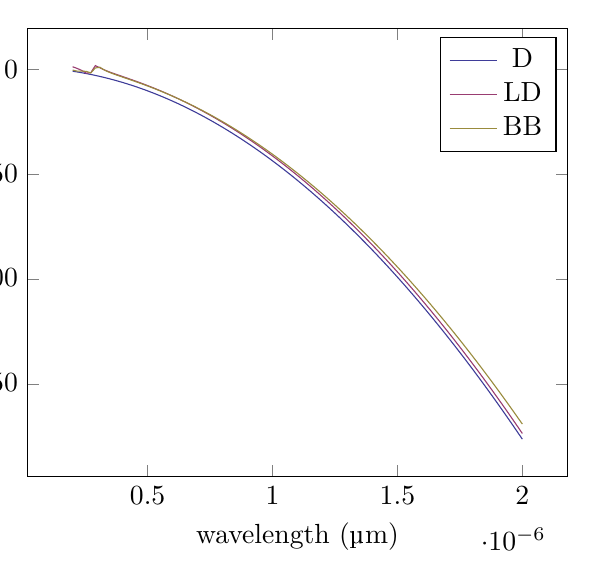
\begin{tikzpicture}[baseline,trim axis left]
\begin{axis}[xlabel=wavelength (\si{\micro\meter}),ylabel=$\epsilon'$]
\addplot[color=colora] coordinates {
(2e-07, -0.78487418047)
(2.18181818182e-07, -1.12412357997)
(2.36363636364e-07, -1.49286415804)
(2.54545454545e-07, -1.89109372276)
(2.72727272727e-07, -2.318809907)
(2.90909090909e-07, -2.77601016848)
(3.09090909091e-07, -3.26269178977)
(3.27272727273e-07, -3.77885187838)
(3.45454545455e-07, -4.32448736675)
(3.63636363636e-07, -4.89959501234)
(3.81818181818e-07, -5.50417139763)
(4e-07, -6.13821293024)
(4.18181818182e-07, -6.8017158429)
(4.36363636364e-07, -7.49467619358)
(4.54545454545e-07, -8.21708986551)
(4.72727272727e-07, -8.96895256725)
(4.90909090909e-07, -9.75025983273)
(5.09090909091e-07, -10.5610070214)
(5.27272727273e-07, -11.4011893181)
(5.45454545455e-07, -12.2708017335)
(5.63636363636e-07, -13.1698391036)
(5.81818181818e-07, -14.0982960906)
(6e-07, -15.0561671821)
(6.18181818182e-07, -16.0434466919)
(6.36363636364e-07, -17.0601287597)
(6.54545454545e-07, -18.1062073511)
(6.72727272727e-07, -19.1816762582)
(6.90909090909e-07, -20.2865290992)
(7.09090909091e-07, -21.4207593186)
(7.27272727273e-07, -22.5843601874)
(7.45454545455e-07, -23.7773248032)
(7.63636363636e-07, -24.9996460903)
(7.81818181818e-07, -26.2513167996)
(8e-07, -27.532329509)
(8.18181818182e-07, -28.8426766233)
(8.36363636364e-07, -30.1823503745)
(8.54545454545e-07, -31.5513428216)
(8.72727272727e-07, -32.9496458512)
(8.90909090909e-07, -34.3772511772)
(9.09090909091e-07, -35.8341503409)
(9.27272727273e-07, -37.3203347117)
(9.45454545455e-07, -38.8357954863)
(9.63636363636e-07, -40.3805236899)
(9.81818181818e-07, -41.9545101754)
(1e-06, -43.5577456239)
(1.01818181818e-06, -45.1902205452)
(1.03636363636e-06, -46.8519252773)
(1.05454545455e-06, -48.5428499868)
(1.07272727273e-06, -50.2629846694)
(1.09090909091e-06, -52.0123191493)
(1.10909090909e-06, -53.7908430802)
(1.12727272727e-06, -55.5985459448)
(1.14545454545e-06, -57.4354170551)
(1.16363636364e-06, -59.3014455529)
(1.18181818182e-06, -61.1966204096)
(1.2e-06, -63.1209304264)
(1.21818181818e-06, -65.0743642346)
(1.23636363636e-06, -67.0569102956)
(1.25454545455e-06, -69.0685569014)
(1.27272727273e-06, -71.1092921742)
(1.29090909091e-06, -73.1791040674)
(1.30909090909e-06, -75.2779803647)
(1.32727272727e-06, -77.4059086814)
(1.34545454545e-06, -79.5628764638)
(1.36363636364e-06, -81.7488709896)
(1.38181818182e-06, -83.9638793683)
(1.4e-06, -86.2078885411)
(1.41818181818e-06, -88.4808852813)
(1.43636363636e-06, -90.7828561942)
(1.45454545455e-06, -93.1137877177)
(1.47272727273e-06, -95.4736661223)
(1.49090909091e-06, -97.8624775112)
(1.50909090909e-06, -100.280207821)
(1.52727272727e-06, -102.72684282)
(1.54545454545e-06, -105.202368112)
(1.56363636364e-06, -107.706769134)
(1.58181818182e-06, -110.240031155)
(1.6e-06, -112.802139281)
(1.61818181818e-06, -115.393078449)
(1.63636363636e-06, -118.012833434)
(1.65454545455e-06, -120.661388842)
(1.67272727273e-06, -123.338729117)
(1.69090909091e-06, -126.044838536)
(1.70909090909e-06, -128.779701214)
(1.72727272727e-06, -131.543301099)
(1.74545454545e-06, -134.335621976)
(1.76363636364e-06, -137.156647466)
(1.78181818182e-06, -140.006361026)
(1.8e-06, -142.884745951)
(1.81818181818e-06, -145.791785371)
(1.83636363636e-06, -148.727462254)
(1.85454545455e-06, -151.691759405)
(1.87272727273e-06, -154.684659466)
(1.89090909091e-06, -157.70614492)
(1.90909090909e-06, -160.756198083)
(1.92727272727e-06, -163.834801113)
(1.94545454545e-06, -166.941936005)
(1.96363636364e-06, -170.077584594)
(1.98181818182e-06, -173.241728554)
(2e-06, -176.434349397)
};
\addlegendentry{D}
\addplot[color=colorb] coordinates {
(2e-07, 1.35905059416)
(2.18181818182e-07, 0.550331143561)
(2.36363636364e-07, -0.401215462349)
(2.54545454545e-07, -1.69666894637)
(2.72727272727e-07, -1.47353407777)
(2.90909090909e-07, 1.91584883134)
(3.09090909091e-07, 0.858580330628)
(3.27272727273e-07, -0.176281144322)
(3.45454545455e-07, -1.03861711603)
(3.63636363636e-07, -1.82120810677)
(3.81818181818e-07, -2.57181745556)
(4e-07, -3.31432340551)
(4.18181818182e-07, -4.06164464627)
(4.36363636364e-07, -4.82132528813)
(4.54545454545e-07, -5.59805997105)
(4.72727272727e-07, -6.39492566494)
(4.90909090909e-07, -7.2140267208)
(5.09090909091e-07, -8.05685394607)
(5.27272727273e-07, -8.9244951388)
(5.45454545455e-07, -9.81776410752)
(5.63636363636e-07, -10.7372827926)
(5.81818181818e-07, -11.6835352791)
(6e-07, -12.656904353)
(6.18181818182e-07, -13.6576968733)
(6.36363636364e-07, -14.6861617783)
(6.54545454545e-07, -15.7425031216)
(6.72727272727e-07, -16.8268896787)
(6.90909090909e-07, -17.939462142)
(7.09090909091e-07, -19.0803385877)
(7.27272727273e-07, -20.249618686)
(7.45454545455e-07, -21.4473869825)
(7.63636363636e-07, -22.6737154835)
(7.81818181818e-07, -23.9286657153)
(8e-07, -25.212290378)
(8.18181818182e-07, -26.5246346866)
(8.36363636364e-07, -27.8657374669)
(8.54545454545e-07, -29.235632057)
(8.72727272727e-07, -30.6343470547)
(8.90909090909e-07, -32.0619069413)
(9.09090909091e-07, -33.5183326047)
(9.27272727273e-07, -35.0036417802)
(9.45454545455e-07, -36.5178494255)
(9.63636363636e-07, -38.0609680398)
(9.81818181818e-07, -39.6330079361)
(1e-06, -41.2339774773)
(1.01818181818e-06, -42.8638832778)
(1.03636363636e-06, -44.5227303801)
(1.05454545455e-06, -46.210522407)
(1.07272727273e-06, -47.9272616954)
(1.09090909091e-06, -49.6729494128)
(1.10909090909e-06, -51.4475856597)
(1.12727272727e-06, -53.2511695602)
(1.14545454545e-06, -55.0836993415)
(1.16363636364e-06, -56.9451724046)
(1.18181818182e-06, -58.8355853867)
(1.2e-06, -60.7549342174)
(1.21818181818e-06, -62.7032141678)
(1.23636363636e-06, -64.6804198954)
(1.25454545455e-06, -66.6865454836)
(1.27272727273e-06, -68.7215844776)
(1.29090909091e-06, -70.7855299162)
(1.30909090909e-06, -72.8783743611)
(1.32727272727e-06, -75.0001099226)
(1.34545454545e-06, -77.1507282834)
(1.36363636364e-06, -79.3302207196)
(1.38181818182e-06, -81.5385781207)
(1.4e-06, -83.7757910066)
(1.41818181818e-06, -86.0418495437)
(1.43636363636e-06, -88.3367435597)
(1.45454545455e-06, -90.6604625566)
(1.47272727273e-06, -93.0129957231)
(1.49090909091e-06, -95.3943319455)
(1.50909090909e-06, -97.8044598181)
(1.52727272727e-06, -100.243367652)
(1.54545454545e-06, -102.711043485)
(1.56363636364e-06, -105.207475087)
(1.58181818182e-06, -107.732649969)
(1.6e-06, -110.286555393)
(1.61818181818e-06, -112.869178369)
(1.63636363636e-06, -115.480505671)
(1.65454545455e-06, -118.120523835)
(1.67272727273e-06, -120.789219169)
(1.69090909091e-06, -123.486577753)
(1.70909090909e-06, -126.212585446)
(1.72727272727e-06, -128.967227891)
(1.74545454545e-06, -131.750490514)
(1.76363636364e-06, -134.562358531)
(1.78181818182e-06, -137.402816952)
(1.8e-06, -140.271850581)
(1.81818181818e-06, -143.169444021)
(1.83636363636e-06, -146.095581674)
(1.85454545455e-06, -149.050247748)
(1.87272727273e-06, -152.033426252)
(1.89090909091e-06, -155.045101007)
(1.90909090909e-06, -158.08525564)
(1.92727272727e-06, -161.153873592)
(1.94545454545e-06, -164.250938115)
(1.96363636364e-06, -167.376432278)
(1.98181818182e-06, -170.530338963)
(2e-06, -173.712640872)
};
\addlegendentry{LD}
\addplot[color=colorc] coordinates {
(2e-07, -0.247217875147)
(2.18181818182e-07, -0.741091026792)
(2.36363636364e-07, -0.693905648861)
(2.54545454545e-07, -0.863316785951)
(2.72727272727e-07, -1.57071009976)
(2.90909090909e-07, 0.779270341698)
(3.09090909091e-07, 1.11053219674)
(3.27272727273e-07, -0.23106368434)
(3.45454545455e-07, -1.24507591502)
(3.63636363636e-07, -2.07675287028)
(3.81818181818e-07, -2.84682061258)
(4e-07, -3.5938063176)
(4.18181818182e-07, -4.33565854094)
(4.36363636364e-07, -5.08287579503)
(4.54545454545e-07, -5.84215676472)
(4.72727272727e-07, -6.61795868206)
(4.90909090909e-07, -7.41333250166)
(5.09090909091e-07, -8.23041702509)
(5.27272727273e-07, -9.07074472552)
(5.45454545455e-07, -9.93543609128)
(5.63636363636e-07, -10.8253257289)
(5.81818181818e-07, -11.7410458102)
(6e-07, -12.6830823777)
(6.18181818182e-07, -13.6518140768)
(6.36363636364e-07, -14.6475393019)
(6.54545454545e-07, -15.6704955671)
(6.72727272727e-07, -16.7208735619)
(6.90909090909e-07, -17.7988275102)
(7.09090909091e-07, -18.9044829163)
(7.27272727273e-07, -20.0379424321)
(7.45454545455e-07, -21.1992903549)
(7.63636363636e-07, -22.3885961138)
(7.81818181818e-07, -23.6059169982)
(8e-07, -24.8513003126)
(8.18181818182e-07, -26.1247850934)
(8.36363636364e-07, -27.4264034856)
(8.54545454545e-07, -28.7561818559)
(8.72727272727e-07, -30.1141416975)
(8.90909090909e-07, -31.5003003706)
(9.09090909091e-07, -32.9146717116)
(9.27272727273e-07, -34.3572665368)
(9.45454545455e-07, -35.8280930609)
(9.63636363636e-07, -37.3271572465)
(9.81818181818e-07, -38.8544630973)
(1e-06, -40.4100129045)
(1.01818181818e-06, -41.993807455)
(1.03636363636e-06, -43.605846209)
(1.05454545455e-06, -45.2461274494)
(1.07272727273e-06, -46.9146484111)
(1.09090909091e-06, -48.6114053908)
(1.10909090909e-06, -50.3363938415)
(1.12727272727e-06, -52.089608454)
(1.14545454545e-06, -53.8710432278)
(1.16363636364e-06, -55.6806915316)
(1.18181818182e-06, -57.5185461564)
(1.2e-06, -59.3845993622)
(1.21818181818e-06, -61.2788429178)
(1.23636363636e-06, -63.2012681364)
(1.25454545455e-06, -65.1518659066)
(1.27272727273e-06, -67.1306267195)
(1.29090909091e-06, -69.1375406927)
(1.30909090909e-06, -71.1725975915)
(1.32727272727e-06, -73.235786848)
(1.34545454545e-06, -75.3270975771)
(1.36363636364e-06, -77.4465185918)
(1.38181818182e-06, -79.5940384162)
(1.4e-06, -81.769645297)
(1.41818181818e-06, -83.9733272142)
(1.43636363636e-06, -86.2050718906)
(1.45454545455e-06, -88.4648668)
(1.47272727273e-06, -90.7526991747)
(1.49090909091e-06, -93.0685560124)
(1.50909090909e-06, -95.4124240826)
(1.52727272727e-06, -97.7842899316)
(1.54545454545e-06, -100.184139888)
(1.56363636364e-06, -102.611960067)
(1.58181818182e-06, -105.067736374)
(1.6e-06, -107.551454511)
(1.61818181818e-06, -110.063099975)
(1.63636363636e-06, -112.602658066)
(1.65454545455e-06, -115.170113887)
(1.67272727273e-06, -117.765452349)
(1.69090909091e-06, -120.388658171)
(1.70909090909e-06, -123.039715882)
(1.72727272727e-06, -125.718609827)
(1.74545454545e-06, -128.425324163)
(1.76363636364e-06, -131.159842866)
(1.78181818182e-06, -133.922149729)
(1.8e-06, -136.712228368)
(1.81818181818e-06, -139.530062216)
(1.83636363636e-06, -142.375634531)
(1.85454545455e-06, -145.248928396)
(1.87272727273e-06, -148.149926716)
(1.89090909091e-06, -151.078612225)
(1.90909090909e-06, -154.034967482)
(1.92727272727e-06, -157.018974875)
(1.94545454545e-06, -160.030616622)
(1.96363636364e-06, -163.069874768)
(1.98181818182e-06, -166.13673119)
(2e-06, -169.231167598)
};
\addlegendentry{BB}
\end{axis}
\end{tikzpicture}%
\\
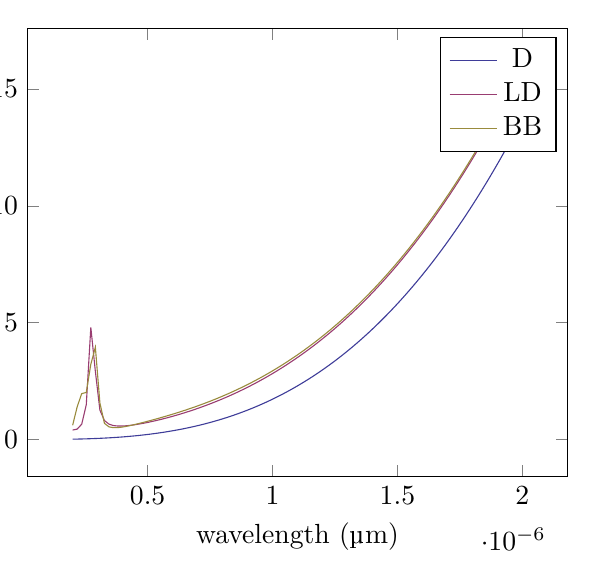
\begin{tikzpicture}[baseline,trim axis left]
\begin{axis}[xlabel=wavelength (\si{\micro\meter}),ylabel=$\epsilon''$]
\addplot[color=colora] coordinates {
(2e-07, 0.0138201424947)
(2.18181818182e-07, 0.0179420992488)
(2.36363636364e-07, 0.0228115184097)
(2.54545454545e-07, 0.0284906550796)
(2.72727272727e-07, 0.0350417563395)
(2.90909090909e-07, 0.0425270606326)
(3.09090909091e-07, 0.0510087971485)
(3.27272727273e-07, 0.060549185207)
(3.45454545455e-07, 0.0712104336428)
(3.63636363636e-07, 0.0830547401899)
(3.81818181818e-07, 0.0961442908663)
(4e-07, 0.110541259359)
(4.18181818182e-07, 0.126307806411)
(4.36363636364e-07, 0.143506079203)
(4.54545454545e-07, 0.162198210743)
(4.72727272727e-07, 0.18244631925)
(4.90909090909e-07, 0.204312507544)
(5.09090909091e-07, 0.227858862427)
(5.27272727273e-07, 0.253147454075)
(5.45454545455e-07, 0.280240335424)
(5.63636363636e-07, 0.309199541558)
(5.81818181818e-07, 0.340087089095)
(6e-07, 0.372964975578)
(6.18181818182e-07, 0.407895178866)
(6.36363636364e-07, 0.444939656516)
(6.54545454545e-07, 0.484160345182)
(6.72727272727e-07, 0.525619159998)
(6.90909090909e-07, 0.569377993971)
(7.09090909091e-07, 0.615498717375)
(7.27272727273e-07, 0.664043177138)
(7.45454545455e-07, 0.715073196237)
(7.63636363636e-07, 0.768650573089)
(7.81818181818e-07, 0.824837080947)
(8e-07, 0.883694467288)
(8.18181818182e-07, 0.945284453214)
(8.36363636364e-07, 1.00966873284)
(8.54545454545e-07, 1.0769089727)
(8.72727272727e-07, 1.14706681112)
(8.90909090909e-07, 1.22020385765)
(9.09090909091e-07, 1.29638169242)
(9.27272727273e-07, 1.37566186558)
(9.45454545455e-07, 1.45810589666)
(9.63636363636e-07, 1.54377527398)
(9.81818181818e-07, 1.63273145409)
(1e-06, 1.72503586109)
(1.01818181818e-06, 1.8207498861)
(1.03636363636e-06, 1.91993488664)
(1.05454545455e-06, 2.02265218603)
(1.07272727273e-06, 2.12896307277)
(1.09090909091e-06, 2.2389288)
(1.10909090909e-06, 2.35261058484)
(1.12727272727e-06, 2.47006960784)
(1.14545454545e-06, 2.59136701239)
(1.16363636364e-06, 2.71656390406)
(1.18181818182e-06, 2.84572135011)
(1.2e-06, 2.97890037881)
(1.21818181818e-06, 3.11616197889)
(1.23636363636e-06, 3.25756709894)
(1.25454545455e-06, 3.40317664684)
(1.27272727273e-06, 3.55305148913)
(1.29090909091e-06, 3.70725245046)
(1.30909090909e-06, 3.865840313)
(1.32727272727e-06, 4.02887581582)
(1.34545454545e-06, 4.19641965436)
(1.36363636364e-06, 4.36853247978)
(1.38181818182e-06, 4.54527489844)
(1.4e-06, 4.72670747129)
(1.41818181818e-06, 4.91289071326)
(1.43636363636e-06, 5.10388509273)
(1.45454545455e-06, 5.29975103093)
(1.47272727273e-06, 5.50054890136)
(1.49090909091e-06, 5.70633902919)
(1.50909090909e-06, 5.91718169073)
(1.52727272727e-06, 6.13313711282)
(1.54545454545e-06, 6.35426547227)
(1.56363636364e-06, 6.58062689528)
(1.58181818182e-06, 6.81228145686)
(1.6e-06, 7.04928918029)
(1.61818181818e-06, 7.2917100365)
(1.63636363636e-06, 7.53960394356)
(1.65454545455e-06, 7.79303076604)
(1.67272727273e-06, 8.05205031453)
(1.69090909091e-06, 8.31672234499)
(1.70909090909e-06, 8.58710655823)
(1.72727272727e-06, 8.86326259936)
(1.74545454545e-06, 9.14525005717)
(1.76363636364e-06, 9.43312846363)
(1.78181818182e-06, 9.7269572933)
(1.8e-06, 10.0267959628)
(1.81818181818e-06, 10.3327038301)
(1.83636363636e-06, 10.6447401943)
(1.85454545455e-06, 10.9629642946)
(1.87272727273e-06, 11.2874353104)
(1.89090909091e-06, 11.6182123599)
(1.90909090909e-06, 11.9553545003)
(1.92727272727e-06, 12.2989207269)
(1.94545454545e-06, 12.6489699725)
(1.96363636364e-06, 13.0055611071)
(1.98181818182e-06, 13.3687529372)
(2e-06, 13.738604205)
};
\addlegendentry{D}
\addplot[color=colorb] coordinates {
(2e-07, 0.404835204104)
(2.18181818182e-07, 0.445563994275)
(2.36363636364e-07, 0.656396239051)
(2.54545454545e-07, 1.48626855057)
(2.72727272727e-07, 4.80154843687)
(2.90909090909e-07, 2.9158733781)
(3.09090909091e-07, 1.25770688622)
(3.27272727273e-07, 0.812670594646)
(3.45454545455e-07, 0.656465341454)
(3.63636363636e-07, 0.595583657803)
(3.81818181818e-07, 0.575694904552)
(4e-07, 0.577010883595)
(4.18181818182e-07, 0.59091098259)
(4.36363636364e-07, 0.613131734653)
(4.54545454545e-07, 0.641359319007)
(4.72727272727e-07, 0.6742479666)
(4.90909090909e-07, 0.710973548767)
(5.09090909091e-07, 0.751012240478)
(5.27272727273e-07, 0.794022799913)
(5.45454545455e-07, 0.839780199233)
(5.63636363636e-07, 0.888136315747)
(5.81818181818e-07, 0.938995644509)
(6e-07, 0.992299731026)
(6.18181818182e-07, 1.04801686734)
(6.36363636364e-07, 1.10613507592)
(6.54545454545e-07, 1.16665721078)
(6.72727272727e-07, 1.22959745987)
(6.90909090909e-07, 1.2949787975)
(7.09090909091e-07, 1.36283109573)
(7.27272727273e-07, 1.43318970166)
(7.45454545455e-07, 1.5060943504)
(7.63636363636e-07, 1.58158832386)
(7.81818181818e-07, 1.65971779222)
(8e-07, 1.74053129311)
(8.18181818182e-07, 1.82407931585)
(8.36363636364e-07, 1.91041396673)
(8.54545454545e-07, 1.99958869755)
(8.72727272727e-07, 2.0916580839)
(8.90909090909e-07, 2.18667764293)
(9.09090909091e-07, 2.28470368278)
(9.27272727273e-07, 2.38579317742)
(9.45454545455e-07, 2.49000366223)
(9.63636363636e-07, 2.59739314639)
(9.81818181818e-07, 2.70802003918)
(1e-06, 2.82194308767)
(1.01818181818e-06, 2.93922132392)
(1.03636363636e-06, 3.05991402)
(1.05454545455e-06, 3.18408064966)
(1.07272727273e-06, 3.31178085555)
(1.09090909091e-06, 3.44307442101)
(1.10909090909e-06, 3.57802124591)
(1.12727272727e-06, 3.71668132574)
(1.14545454545e-06, 3.85911473355)
(1.16363636364e-06, 4.00538160434)
(1.18181818182e-06, 4.15554212148)
(1.2e-06, 4.3096565049)
(1.21818181818e-06, 4.4677850008)
(1.23636363636e-06, 4.62998787266)
(1.25454545455e-06, 4.79632539334)
(1.27272727273e-06, 4.96685783824)
(1.29090909091e-06, 5.14164547918)
(1.30909090909e-06, 5.32074857907)
(1.32727272727e-06, 5.50422738718)
(1.34545454545e-06, 5.69214213501)
(1.36363636364e-06, 5.88455303253)
(1.38181818182e-06, 6.08152026492)
(1.4e-06, 6.28310398966)
(1.41818181818e-06, 6.48936433385)
(1.43636363636e-06, 6.70036139195)
(1.45454545455e-06, 6.91615522357)
(1.47272727273e-06, 7.13680585165)
(1.49090909091e-06, 7.36237326071)
(1.50909090909e-06, 7.59291739526)
(1.52727272727e-06, 7.82849815844)
(1.54545454545e-06, 8.06917541066)
(1.56363636364e-06, 8.31500896847)
(1.58181818182e-06, 8.56605860337)
(1.6e-06, 8.8223840409)
(1.61818181818e-06, 9.08404495959)
(1.63636363636e-06, 9.35110099016)
(1.65454545455e-06, 9.62361171463)
(1.67272727273e-06, 9.90163666558)
(1.69090909091e-06, 10.1852353254)
(1.70909090909e-06, 10.4744671255)
(1.72727272727e-06, 10.7693914458)
(1.74545454545e-06, 11.0700676141)
(1.76363636364e-06, 11.3765549051)
(1.78181818182e-06, 11.6889125403)
(1.8e-06, 12.0071996871)
(1.81818181818e-06, 12.3314754584)
(1.83636363636e-06, 12.6617989119)
(1.85454545455e-06, 12.9982290496)
(1.87272727273e-06, 13.3408248173)
(1.89090909091e-06, 13.6896451043)
(1.90909090909e-06, 14.0447487425)
(1.92727272727e-06, 14.4061945061)
(1.94545454545e-06, 14.7740411109)
(1.96363636364e-06, 15.1483472144)
(1.98181818182e-06, 15.5291714144)
(2e-06, 15.9165722493)
};
\addlegendentry{LD}
\addplot[color=colorc] coordinates {
(2e-07, 0.610290444635)
(2.18181818182e-07, 1.40252802297)
(2.36363636364e-07, 1.96471721824)
(2.54545454545e-07, 2.01410693801)
(2.72727272727e-07, 3.21868133765)
(2.90909090909e-07, 3.94982741168)
(3.09090909091e-07, 1.56281316342)
(3.27272727273e-07, 0.690954401027)
(3.45454545455e-07, 0.540471967881)
(3.63636363636e-07, 0.505730119371)
(3.81818181818e-07, 0.509772747333)
(4e-07, 0.534094289304)
(4.18181818182e-07, 0.569522040049)
(4.36363636364e-07, 0.611215461009)
(4.54545454545e-07, 0.656652635702)
(4.72727272727e-07, 0.704543149633)
(4.90909090909e-07, 0.754247268071)
(5.09090909091e-07, 0.805469614139)
(5.27272727273e-07, 0.858097996433)
(5.45454545455e-07, 0.912118141851)
(5.63636363636e-07, 0.967568119279)
(5.81818181818e-07, 1.02451367233)
(6e-07, 1.08303470336)
(6.18181818182e-07, 1.14321779585)
(6.36363636364e-07, 1.20515206059)
(6.54545454545e-07, 1.26892684131)
(6.72727272727e-07, 1.33463047558)
(6.90909090909e-07, 1.40234966121)
(7.09090909091e-07, 1.47216917203)
(7.27272727273e-07, 1.54417177476)
(7.45454545455e-07, 1.61843825991)
(7.63636363636e-07, 1.69504753497)
(7.81818181818e-07, 1.7740767491)
(8e-07, 1.85560143072)
(8.18181818182e-07, 1.93969562726)
(8.36363636364e-07, 2.02643204074)
(8.54545454545e-07, 2.11588215563)
(8.72727272727e-07, 2.20811635738)
(8.90909090909e-07, 2.30320404104)
(9.09090909091e-07, 2.40121370976)
(9.27272727273e-07, 2.50221306382)
(9.45454545455e-07, 2.60626908056)
(9.63636363636e-07, 2.71344808606)
(9.81818181818e-07, 2.82381581921)
(1e-06, 2.93743748888)
(1.01818181818e-06, 3.0543778249)
(1.03636363636e-06, 3.17470112354)
(1.05454545455e-06, 3.29847128792)
(1.07272727273e-06, 3.42575186413)
(1.09090909091e-06, 3.55660607328)
(1.10909090909e-06, 3.69109684009)
(1.12727272727e-06, 3.82928681836)
(1.14545454545e-06, 3.97123841368)
(1.16363636364e-06, 4.11701380366)
(1.18181818182e-06, 4.26667495593)
(1.2e-06, 4.42028364425)
(1.21818181818e-06, 4.57790146286)
(1.23636363636e-06, 4.73958983933)
(1.25454545455e-06, 4.90541004591)
(1.27272727273e-06, 5.07542320985)
(1.29090909091e-06, 5.24969032247)
(1.30909090909e-06, 5.4282722473)
(1.32727272727e-06, 5.61122972744)
(1.34545454545e-06, 5.79862339198)
(1.36363636364e-06, 5.99051376189)
(1.38181818182e-06, 6.18696125518)
(1.4e-06, 6.38802619155)
(1.41818181818e-06, 6.59376879654)
(1.43636363636e-06, 6.80424920522)
(1.45454545455e-06, 7.01952746549)
(1.47272727273e-06, 7.239663541)
(1.49090909091e-06, 7.46471731378)
(1.50909090909e-06, 7.69474858653)
(1.52727272727e-06, 7.92981708472)
(1.54545454545e-06, 8.16998245836)
(1.56363636364e-06, 8.41530428362)
(1.58181818182e-06, 8.66584206427)
(1.6e-06, 8.92165523284)
(1.61818181818e-06, 9.1828031518)
(1.63636363636e-06, 9.44934511439)
(1.65454545455e-06, 9.72134034551)
(1.67272727273e-06, 9.99884800237)
(1.69090909091e-06, 10.281927175)
(1.70909090909e-06, 10.570636887)
(1.72727272727e-06, 10.8650360955)
(1.74545454545e-06, 11.1651836918)
(1.76363636364e-06, 11.4711385016)
(1.78181818182e-06, 11.7829592851)
(1.8e-06, 12.100704737)
(1.81818181818e-06, 12.4244334869)
(1.83636363636e-06, 12.7542040989)
(1.85454545455e-06, 13.0900750719)
(1.87272727273e-06, 13.4321048393)
(1.89090909091e-06, 13.780351769)
(1.90909090909e-06, 14.1348741633)
(1.92727272727e-06, 14.4957302586)
(1.94545454545e-06, 14.8629782253)
(1.96363636364e-06, 15.2366761674)
(1.98181818182e-06, 15.6168821224)
(2e-06, 16.003654061)
};
\addlegendentry{BB}
\end{axis}
\end{tikzpicture}%
\\
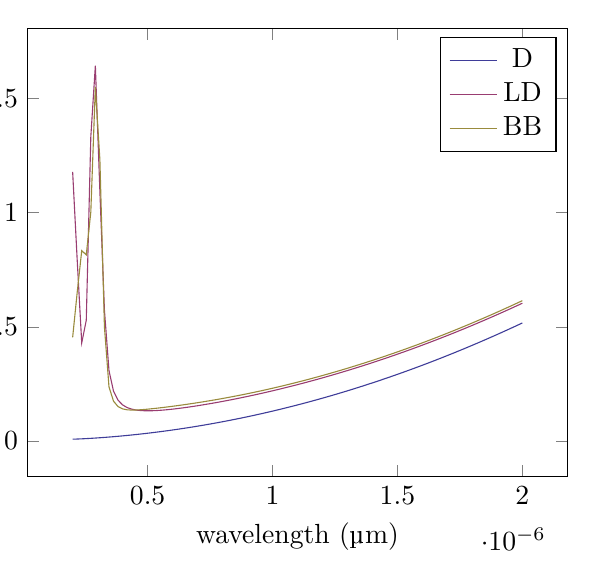
\begin{tikzpicture}[baseline,trim axis left]
\begin{axis}[xlabel=wavelength (\si{\micro\meter}),ylabel=$n'$]
\addplot[color=colora] coordinates {
(2e-07, 0.00779948046325)
(2.18181818182e-07, 0.0084610137681)
(2.36363636364e-07, 0.00933472178687)
(2.54545454545e-07, 0.0103586603228)
(2.72727272727e-07, 0.011505643138)
(2.90909090909e-07, 0.0127618050235)
(3.09090909091e-07, 0.0141193204209)
(3.27272727273e-07, 0.0155734357984)
(3.45454545455e-07, 0.0171210974727)
(3.63636363636e-07, 0.0187602550701)
(3.81818181818e-07, 0.0204894815024)
(4e-07, 0.0223077533364)
(4.18181818182e-07, 0.0242143177378)
(4.36363636364e-07, 0.026208608632)
(4.54545454545e-07, 0.0282901920844)
(4.72727272727e-07, 0.0304587296862)
(4.90909090909e-07, 0.0327139533895)
(5.09090909091e-07, 0.0350556478318)
(5.27272727273e-07, 0.0374836376781)
(5.45454545455e-07, 0.0399977783993)
(5.63636363636e-07, 0.0425979494493)
(5.81818181818e-07, 0.0452840491467)
(6e-07, 0.0480559907853)
(6.18181818182e-07, 0.0509136996457)
(6.36363636364e-07, 0.0538571106734)
(6.54545454545e-07, 0.0568861666576)
(6.72727272727e-07, 0.0600008167913)
(6.90909090909e-07, 0.0632010155208)
(7.09090909091e-07, 0.066486721622)
(7.27272727273e-07, 0.0698578974514)
(7.45454545455e-07, 0.0733145083363)
(7.63636363636e-07, 0.076856522074)
(7.81818181818e-07, 0.0804839085185)
(8e-07, 0.0841966392385)
(8.18181818182e-07, 0.087994687231)
(8.36363636364e-07, 0.0918780266819)
(8.54545454545e-07, 0.0958466327646)
(8.72727272727e-07, 0.0999004814692)
(8.90909090909e-07, 0.104039549458)
(9.09090909091e-07, 0.108263813942)
(9.27272727273e-07, 0.112573252574)
(9.45454545455e-07, 0.116967843362)
(9.63636363636e-07, 0.121447564584)
(9.81818181818e-07, 0.12601239473)
(1e-06, 0.130662312433)
(1.01818181818e-06, 0.135397296428)
(1.03636363636e-06, 0.140217325498)
(1.05454545455e-06, 0.145122378446)
(1.07272727273e-06, 0.15011243405)
(1.09090909091e-06, 0.155187471042)
(1.10909090909e-06, 0.160347468076)
(1.12727272727e-06, 0.165592403708)
(1.14545454545e-06, 0.170922256375)
(1.16363636364e-06, 0.176337004374)
(1.18181818182e-06, 0.181836625851)
(1.2e-06, 0.187421098782)
(1.21818181818e-06, 0.193090400962)
(1.23636363636e-06, 0.198844509995)
(1.25454545455e-06, 0.204683403282)
(1.27272727273e-06, 0.210607058011)
(1.29090909091e-06, 0.216615451152)
(1.30909090909e-06, 0.222708559448)
(1.32727272727e-06, 0.228886359406)
(1.34545454545e-06, 0.235148827296)
(1.36363636364e-06, 0.241495939142)
(1.38181818182e-06, 0.247927670719)
(1.4e-06, 0.254443997547)
(1.41818181818e-06, 0.261044894888)
(1.43636363636e-06, 0.267730337745)
(1.45454545455e-06, 0.274500300852)
(1.47272727273e-06, 0.281354758681)
(1.49090909091e-06, 0.288293685429)
(1.50909090909e-06, 0.295317055024)
(1.52727272727e-06, 0.302424841117)
(1.54545454545e-06, 0.309617017085)
(1.56363636364e-06, 0.316893556025)
(1.58181818182e-06, 0.324254430756)
(1.6e-06, 0.331699613815)
(1.61818181818e-06, 0.339229077455)
(1.63636363636e-06, 0.346842793649)
(1.65454545455e-06, 0.354540734083)
(1.67272727273e-06, 0.362322870158)
(1.69090909091e-06, 0.37018917299)
(1.70909090909e-06, 0.378139613407)
(1.72727272727e-06, 0.386174161949)
(1.74545454545e-06, 0.394292788868)
(1.76363636364e-06, 0.402495464129)
(1.78181818182e-06, 0.410782157407)
(1.8e-06, 0.419152838086)
(1.81818181818e-06, 0.427607475262)
(1.83636363636e-06, 0.436146037741)
(1.85454545455e-06, 0.444768494037)
(1.87272727273e-06, 0.453474812376)
(1.89090909091e-06, 0.462264960692)
(1.90909090909e-06, 0.471138906628)
(1.92727272727e-06, 0.480096617537)
(1.94545454545e-06, 0.489138060481)
(1.96363636364e-06, 0.498263202231)
(1.98181818182e-06, 0.507472009267)
(2e-06, 0.51676444778)
};
\addlegendentry{D}
\addplot[color=colorb] coordinates {
(2e-07, 1.1783709516)
(2.18181818182e-07, 0.793227987236)
(2.36363636364e-07, 0.429004273941)
(2.54545454545e-07, 0.528639577639)
(2.72727272727e-07, 1.3321096063)
(2.90909090909e-07, 1.64389811313)
(3.09090909091e-07, 1.09119253913)
(3.27272727273e-07, 0.572402296869)
(3.45454545455e-07, 0.308277548036)
(3.63636363636e-07, 0.217844758879)
(3.81818181818e-07, 0.178390559815)
(4e-07, 0.157880886481)
(4.18181818182e-07, 0.146218081028)
(4.36363636364e-07, 0.139337466953)
(4.54545454545e-07, 0.135314258326)
(4.72727272727e-07, 0.133128463642)
(4.90909090909e-07, 0.132193225472)
(5.09090909091e-07, 0.132149070617)
(5.27272727273e-07, 0.13276472234)
(5.45454545455e-07, 0.133885403463)
(5.63636363636e-07, 0.135404147434)
(5.81818181818e-07, 0.137245034925)
(6e-07, 0.139352966827)
(6.18181818182e-07, 0.141687192412)
(6.36363636364e-07, 0.144217083237)
(6.54545454545e-07, 0.146919297527)
(6.72727272727e-07, 0.149775831908)
(6.90909090909e-07, 0.152772654685)
(7.09090909091e-07, 0.155898729286)
(7.27272727273e-07, 0.159145305043)
(7.45454545455e-07, 0.162505394569)
(7.63636363636e-07, 0.165973383591)
(7.81818181818e-07, 0.169544736257)
(8e-07, 0.173215770174)
(8.18181818182e-07, 0.176983483041)
(8.36363636364e-07, 0.180845417877)
(8.54545454545e-07, 0.184799557417)
(8.72727272727e-07, 0.188844240769)
(8.90909090909e-07, 0.1929780972)
(9.09090909091e-07, 0.19719999321)
(9.27272727273e-07, 0.20150899)
(9.45454545455e-07, 0.205904309097)
(9.63636363636e-07, 0.210385304466)
(9.81818181818e-07, 0.21495143976)
(1e-06, 0.219602269704)
(1.01818181818e-06, 0.224337424795)
(1.03636363636e-06, 0.22915659869)
(1.05454545455e-06, 0.234059537771)
(1.07272727273e-06, 0.239046032485)
(1.09090909091e-06, 0.244115910147)
(1.10909090909e-06, 0.24926902893)
(1.12727272727e-06, 0.254505272844)
(1.14545454545e-06, 0.259824547531)
(1.16363636364e-06, 0.26522677673)
(1.18181818182e-06, 0.270711899313)
(1.2e-06, 0.276279866779)
(1.21818181818e-06, 0.281930641148)
(1.23636363636e-06, 0.287664193178)
(1.25454545455e-06, 0.293480500862)
(1.27272727273e-06, 0.29937954815)
(1.29090909091e-06, 0.305361323874)
(1.30909090909e-06, 0.311425820834)
(1.32727272727e-06, 0.317573035022)
(1.34545454545e-06, 0.323802964967)
(1.36363636364e-06, 0.330115611179)
(1.38181818182e-06, 0.336510975681)
(1.4e-06, 0.342989061606)
(1.41818181818e-06, 0.349549872862)
(1.43636363636e-06, 0.35619341385)
(1.45454545455e-06, 0.362919689222)
(1.47272727273e-06, 0.369728703678)
(1.49090909091e-06, 0.376620461801)
(1.50909090909e-06, 0.383594967913)
(1.52727272727e-06, 0.390652225958)
(1.54545454545e-06, 0.397792239403)
(1.56363636364e-06, 0.405015011162)
(1.58181818182e-06, 0.412320543526)
(1.6e-06, 0.419708838114)
(1.61818181818e-06, 0.427179895829)
(1.63636363636e-06, 0.434733716824)
(1.65454545455e-06, 0.44237030048)
(1.67272727273e-06, 0.450089645384)
(1.69090909091e-06, 0.45789174932)
(1.70909090909e-06, 0.465776609254)
(1.72727272727e-06, 0.473744221337)
(1.74545454545e-06, 0.481794580899)
(1.76363636364e-06, 0.489927682455)
(1.78181818182e-06, 0.498143519702)
(1.8e-06, 0.506442085533)
(1.81818181818e-06, 0.514823372039)
(1.83636363636e-06, 0.52328737052)
(1.85454545455e-06, 0.531834071495)
(1.87272727273e-06, 0.540463464709)
(1.89090909091e-06, 0.54917553915)
(1.90909090909e-06, 0.557970283057)
(1.92727272727e-06, 0.566847683931)
(1.94545454545e-06, 0.575807728549)
(1.96363636364e-06, 0.584850402978)
(1.98181818182e-06, 0.593975692581)
(2e-06, 0.603183582037)
};
\addlegendentry{LD}
\addplot[color=colorc] coordinates {
(2e-07, 0.453455228736)
(2.18181818182e-07, 0.650074681284)
(2.36363636364e-07, 0.833591477964)
(2.54545454545e-07, 0.814867087929)
(2.72727272727e-07, 1.00269027957)
(2.90909090909e-07, 1.55003805134)
(3.09090909091e-07, 1.23039323803)
(3.27272727273e-07, 0.498749592308)
(3.45454545455e-07, 0.236903400673)
(3.63636363636e-07, 0.1741993092)
(3.81818181818e-07, 0.150468786971)
(4e-07, 0.140482235886)
(4.18181818182e-07, 0.136465319873)
(4.36363636364e-07, 0.135309665374)
(4.54545454545e-07, 0.135623980032)
(4.72727272727e-07, 0.136742309277)
(4.90909090909e-07, 0.138330272655)
(5.09090909091e-07, 0.140213609053)
(5.27272727273e-07, 0.142298792411)
(5.45454545455e-07, 0.144534504256)
(5.63636363636e-07, 0.146892179777)
(5.81818181818e-07, 0.14935583646)
(6e-07, 0.151916588689)
(6.18181818182e-07, 0.154569607901)
(6.36363636364e-07, 0.157312398528)
(6.54545454545e-07, 0.160143801761)
(6.72727272727e-07, 0.163063411942)
(6.90909090909e-07, 0.166071231945)
(7.09090909091e-07, 0.169167469451)
(7.27272727273e-07, 0.172352417431)
(7.45454545455e-07, 0.175626385443)
(7.63636363636e-07, 0.178989661717)
(7.81818181818e-07, 0.182442493878)
(8e-07, 0.185985080833)
(8.18181818182e-07, 0.18961757123)
(8.36363636364e-07, 0.193340065622)
(8.54545454545e-07, 0.197152620583)
(8.72727272727e-07, 0.201055253702)
(8.90909090909e-07, 0.205047948798)
(9.09090909091e-07, 0.209130660991)
(9.27272727273e-07, 0.213303321429)
(9.45454545455e-07, 0.217565841549)
(9.63636363636e-07, 0.221918116874)
(9.81818181818e-07, 0.22636003031)
(1e-06, 0.23089145501)
(1.01818181818e-06, 0.235512256806)
(1.03636363636e-06, 0.240222296278)
(1.05454545455e-06, 0.245021430494)
(1.07272727273e-06, 0.24990951445)
(1.09090909091e-06, 0.254886402276)
(1.10909090909e-06, 0.259951948214)
(1.12727272727e-06, 0.265106007413)
(1.14545454545e-06, 0.270348436577)
(1.16363636364e-06, 0.275679094465)
(1.18181818182e-06, 0.281097842291)
(1.2e-06, 0.286604544021)
(1.21818181818e-06, 0.292199066599)
(1.23636363636e-06, 0.297881280098)
(1.25454545455e-06, 0.303651057827)
(1.27272727273e-06, 0.309508276381)
(1.29090909091e-06, 0.315452815665)
(1.30909090909e-06, 0.321484558881)
(1.32727272727e-06, 0.327603392497)
(1.34545454545e-06, 0.333809206187)
(1.36363636364e-06, 0.340101892766)
(1.38181818182e-06, 0.346481348107)
(1.4e-06, 0.352947471052)
(1.41818181818e-06, 0.359500163316)
(1.43636363636e-06, 0.366139329383)
(1.45454545455e-06, 0.372864876404)
(1.47272727273e-06, 0.379676714094)
(1.49090909091e-06, 0.386574754619)
(1.50909090909e-06, 0.393558912498)
(1.52727272727e-06, 0.400629104492)
(1.54545454545e-06, 0.407785249506)
(1.56363636364e-06, 0.415027268486)
(1.58181818182e-06, 0.42235508432)
(1.6e-06, 0.429768621747)
(1.61818181818e-06, 0.437267807259)
(1.63636363636e-06, 0.444852569014)
(1.65454545455e-06, 0.45252283675)
(1.67272727273e-06, 0.460278541703)
(1.69090909091e-06, 0.468119616525)
(1.70909090909e-06, 0.476045995209)
(1.72727272727e-06, 0.484057613015)
(1.74545454545e-06, 0.492154406398)
(1.76363636364e-06, 0.500336312945)
(1.78181818182e-06, 0.508603271306)
(1.8e-06, 0.516955221135)
(1.81818181818e-06, 0.525392103031)
(1.83636363636e-06, 0.53391385848)
(1.85454545455e-06, 0.542520429804)
(1.87272727273e-06, 0.55121176011)
(1.89090909091e-06, 0.559987793239)
(1.90909090909e-06, 0.56884847372)
(1.92727272727e-06, 0.577793746729)
(1.94545454545e-06, 0.586823558042)
(1.96363636364e-06, 0.595937854)
(1.98181818182e-06, 0.605136581467)
(2e-06, 0.614419687795)
};
\addlegendentry{BB}
\end{axis}
\end{tikzpicture}%
\\
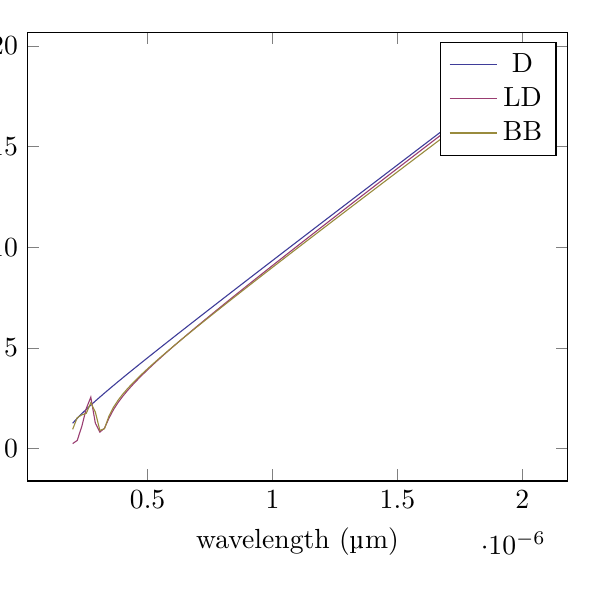
\begin{tikzpicture}[baseline,trim axis left]
\begin{axis}[xlabel=wavelength (\si{\micro\meter}),ylabel=$n''$]
\addplot[color=colora] coordinates {
(2e-07, 1.25294454176)
(2.18181818182e-07, 1.49946334982)
(2.36363636364e-07, 1.72797644375)
(2.54545454545e-07, 1.94483985181)
(2.72727272727e-07, 2.15357483586)
(2.90909090909e-07, 2.35634166968)
(3.09090909091e-07, 2.55456107579)
(3.27272727273e-07, 2.74921603745)
(3.45454545455e-07, 2.94101360035)
(3.63636363636e-07, 3.13047822529)
(3.81818181818e-07, 3.31800880544)
(4e-07, 3.50391511487)
(4.18181818182e-07, 3.68844199523)
(4.36363636364e-07, 3.87178591473)
(4.54545454545e-07, 4.05410660947)
(4.72727272727e-07, 4.23553545646)
(4.90909090909e-07, 4.41618161662)
(5.09090909091e-07, 4.59613662108)
(5.27272727273e-07, 4.77547784859)
(5.45454545455e-07, 4.95427119882)
(5.63636363636e-07, 5.13257317316)
(5.81818181818e-07, 5.31043251265)
(6e-07, 5.48789150045)
(6.18181818182e-07, 5.66498700735)
(6.36363636364e-07, 5.84175133809)
(6.54545454545e-07, 6.01821292197)
(6.72727272727e-07, 6.19439688044)
(6.90909090909e-07, 6.37032549679)
(7.09090909091e-07, 6.54601860717)
(7.27272727273e-07, 6.72149392817)
(7.45454545455e-07, 6.89676733265)
(7.63636363636e-07, 7.07185308322)
(7.81818181818e-07, 7.24676403081)
(8e-07, 7.42151178441)
(8.18181818182e-07, 7.59610685658)
(8.36363636364e-07, 7.77055878895)
(8.54545454545e-07, 7.94487626067)
(8.72727272727e-07, 8.11906718256)
(8.90909090909e-07, 8.29313877914)
(9.09090909091e-07, 8.46709766028)
(9.27272727273e-07, 8.64094988399)
(9.45454545455e-07, 8.81470101169)
(9.63636363636e-07, 8.98835615681)
(9.81818181818e-07, 9.16192002792)
(1e-06, 9.3353969668)
(1.01818181818e-06, 9.50879098236)
(1.03636363636e-06, 9.68210578084)
(1.05454545455e-06, 9.85534479271)
(1.07272727273e-06, 10.0285111968)
(1.09090909091e-06, 10.2016079419)
(1.10909090909e-06, 10.3746377663)
(1.12727272727e-06, 10.5476032148)
(1.14545454545e-06, 10.7205066553)
(1.16363636364e-06, 10.893350292)
(1.18181818182e-06, 11.0661361792)
(1.2e-06, 11.2388662324)
(1.21818181818e-06, 11.4115422391)
(1.23636363636e-06, 11.5841658685)
(1.25454545455e-06, 11.7567386802)
(1.27272727273e-06, 11.929262132)
(1.29090909091e-06, 12.1017375877)
(1.30909090909e-06, 12.2741663234)
(1.32727272727e-06, 12.4465495337)
(1.34545454545e-06, 12.6188883373)
(1.36363636364e-06, 12.7911837825)
(1.38181818182e-06, 12.9634368513)
(1.4e-06, 13.1356484643)
(1.41818181818e-06, 13.3078194847)
(1.43636363636e-06, 13.4799507216)
(1.45454545455e-06, 13.6520429338)
(1.47272727273e-06, 13.8240968329)
(1.49090909091e-06, 13.9961130862)
(1.50909090909e-06, 14.1680923193)
(1.52727272727e-06, 14.3400351188)
(1.54545454545e-06, 14.5119420347)
(1.56363636364e-06, 14.6838135823)
(1.58181818182e-06, 14.8556502444)
(1.6e-06, 15.027452473)
(1.61818181818e-06, 15.1992206916)
(1.63636363636e-06, 15.3709552961)
(1.65454545455e-06, 15.5426566567)
(1.67272727273e-06, 15.7143251194)
(1.69090909091e-06, 15.8859610071)
(1.70909090909e-06, 16.0575646211)
(1.72727272727e-06, 16.2291362421)
(1.74545454545e-06, 16.4006761311)
(1.76363636364e-06, 16.572184531)
(1.78181818182e-06, 16.7436616669)
(1.8e-06, 16.9151077474)
(1.81818181818e-06, 17.0865229654)
(1.83636363636e-06, 17.2579074989)
(1.85454545455e-06, 17.4292615115)
(1.87272727273e-06, 17.6005851534)
(1.89090909091e-06, 17.7718785621)
(1.90909090909e-06, 17.9431418627)
(1.92727272727e-06, 18.1143751686)
(1.94545454545e-06, 18.2855785824)
(1.96363636364e-06, 18.456752196)
(1.98181818182e-06, 18.6278960913)
(2e-06, 18.7990103405)
};
\addlegendentry{D}
\addplot[color=colorb] coordinates {
(2e-07, 0.242930053305)
(2.18181818182e-07, 0.397188862312)
(2.36363636364e-07, 1.08190584563)
(2.54545454545e-07, 1.98802854578)
(2.72727272727e-07, 2.54874482088)
(2.90909090909e-07, 1.25423456738)
(3.09090909091e-07, 0.815010216895)
(3.27272727273e-07, 1.00391785897)
(3.45454545455e-07, 1.50575706052)
(3.63636363636e-07, 1.93321723857)
(3.81818181818e-07, 2.2819468212)
(4e-07, 2.58427931146)
(4.18181818182e-07, 2.85762991778)
(4.36363636364e-07, 3.11150774315)
(4.54545454545e-07, 3.35152798573)
(4.72727272727e-07, 3.5812424807)
(4.90909090909e-07, 3.803025577)
(5.09090909091e-07, 4.01853638106)
(5.27272727273e-07, 4.22897661623)
(5.45454545455e-07, 4.43524281382)
(5.63636363636e-07, 4.63802049926)
(5.81818181818e-07, 4.83784486704)
(6e-07, 5.03514122987)
(6.18181818182e-07, 5.23025279193)
(6.36363636364e-07, 5.42346021381)
(6.54545454545e-07, 5.6149957082)
(6.72727272727e-07, 5.8050533983)
(6.90909090909e-07, 5.99379706464)
(7.09090909091e-07, 6.1813660305)
(7.27272727273e-07, 6.36787969644)
(7.45454545455e-07, 6.55344107866)
(7.63636363636e-07, 6.73813960194)
(7.81818181818e-07, 6.92205332729)
(8e-07, 7.10525074589)
(8.18181818182e-07, 7.28779223632)
(8.36363636364e-07, 7.46973125783)
(8.54545454545e-07, 7.65111533482)
(8.72727272727e-07, 7.8319868746)
(8.90909090909e-07, 8.01238385093)
(9.09090909091e-07, 8.19234037891)
(9.27272727273e-07, 8.37188720101)
(9.45454545455e-07, 8.55105210019)
(9.63636363636e-07, 8.72986025273)
(9.81818181818e-07, 8.90833453094)
(1e-06, 9.08649576395)
(1.01818181818e-06, 9.26436296331)
(1.03636363636e-06, 9.44195351893)
(1.05454545455e-06, 9.6192833698)
(1.07272727273e-06, 9.7963671533)
(1.09090909091e-06, 9.97321833616)
(1.10909090909e-06, 10.1498493298)
(1.12727272727e-06, 10.3262715918)
(1.14545454545e-06, 10.5024957164)
(1.16363636364e-06, 10.678531514)
(1.18181818182e-06, 10.8543880822)
(1.2e-06, 11.0300738694)
(1.21818181818e-06, 11.2055967315)
(1.23636363636e-06, 11.3809639823)
(1.25454545455e-06, 11.5561824395)
(1.27272727273e-06, 11.7312584654)
(1.29090909091e-06, 11.9061980039)
(1.30909090909e-06, 12.0810066139)
(1.32727272727e-06, 12.2556894996)
(1.34545454545e-06, 12.4302515376)
(1.36363636364e-06, 12.6046973019)
(1.38181818182e-06, 12.7790310867)
(1.4e-06, 12.9532569266)
(1.41818181818e-06, 13.1273786155)
(1.43636363636e-06, 13.3013997239)
(1.45454545455e-06, 13.4753236145)
(1.47272727273e-06, 13.6491534563)
(1.49090909091e-06, 13.8228922384)
(1.50909090909e-06, 13.9965427815)
(1.52727272727e-06, 14.1701077493)
(1.54545454545e-06, 14.3435896588)
(1.56363636364e-06, 14.5169908897)
(1.58181818182e-06, 14.690313693)
(1.6e-06, 14.8635601994)
(1.61818181818e-06, 15.0367324264)
(1.63636363636e-06, 15.2098322854)
(1.65454545455e-06, 15.382861588)
(1.67272727273e-06, 15.5558220521)
(1.69090909091e-06, 15.7287153072)
(1.70909090909e-06, 15.9015428997)
(1.72727272727e-06, 16.0743062978)
(1.74545454545e-06, 16.2470068955)
(1.76363636364e-06, 16.4196460172)
(1.78181818182e-06, 16.5922249212)
(1.8e-06, 16.7647448037)
(1.81818181818e-06, 16.9372068019)
(1.83636363636e-06, 17.1096119972)
(1.85454545455e-06, 17.281961418)
(1.87272727273e-06, 17.4542560431)
(1.89090909091e-06, 17.6264968034)
(1.90909090909e-06, 17.7986845849)
(1.92727272727e-06, 17.9708202311)
(1.94545454545e-06, 18.1429045445)
(1.96363636364e-06, 18.3149382894)
(1.98181818182e-06, 18.4869221931)
(2e-06, 18.6588569482)
};
\addlegendentry{LD}
\addplot[color=colorc] coordinates {
(2e-07, 0.951671707696)
(2.18181818182e-07, 1.52557406771)
(2.36363636364e-07, 1.66660157266)
(2.54545454545e-07, 1.74775579355)
(2.72727272727e-07, 2.26984488302)
(2.90909090909e-07, 1.8018588285)
(3.09090909091e-07, 0.898148454834)
(3.27272727273e-07, 0.979606900922)
(3.45454545455e-07, 1.61319505099)
(3.63636363636e-07, 2.05285083219)
(3.81818181818e-07, 2.39560492086)
(4e-07, 2.68832348358)
(4.18181818182e-07, 2.95102738871)
(4.36363636364e-07, 3.19411474452)
(4.54545454545e-07, 3.4236093903)
(4.72727272727e-07, 3.64325600012)
(4.90909090909e-07, 3.85550716923)
(5.09090909091e-07, 4.06203812913)
(5.27272727273e-07, 4.26403416305)
(5.45454545455e-07, 4.46235953599)
(5.63636363636e-07, 4.65766100987)
(5.81818181818e-07, 4.85043358393)
(6e-07, 5.04106358374)
(6.18181818182e-07, 5.22985771135)
(6.36363636364e-07, 5.41706313285)
(6.54545454545e-07, 5.60288168791)
(6.72727272727e-07, 5.78748014911)
(6.90909090909e-07, 5.97099776658)
(7.09090909091e-07, 6.15355190911)
(7.27272727273e-07, 6.33524234547)
(7.45454545455e-07, 6.5161545381)
(7.63636363636e-07, 6.69636220837)
(7.81818181818e-07, 6.87592935707)
(8e-07, 7.05491187229)
(8.18181818182e-07, 7.233358821)
(8.36363636364e-07, 7.41131349581)
(8.54545454545e-07, 7.58881426992)
(8.72727272727e-07, 7.76589530093)
(8.90909090909e-07, 7.94258711402)
(9.09090909091e-07, 8.1189170885)
(9.27272727273e-07, 8.29490986614)
(9.45454545455e-07, 8.47058769582)
(9.63636363636e-07, 8.64597072596)
(9.81818181818e-07, 8.82107725402)
(1e-06, 8.99592394015)
(1.01818181818e-06, 9.17052599126)
(1.03636363636e-06, 9.34489731999)
(1.05454545455e-06, 9.51905068279)
(1.07272727273e-06, 9.69299780012)
(1.09090909091e-06, 9.86674946159)
(1.10909090909e-06, 10.0403156182)
(1.12727272727e-06, 10.2137054637)
(1.14545454545e-06, 10.3869275058)
(1.16363636364e-06, 10.5599896302)
(1.18181818182e-06, 10.7328991566)
(1.2e-06, 10.9056628892)
(1.21818181818e-06, 11.0782871611)
(1.23636363636e-06, 11.2507778747)
(1.25454545455e-06, 11.4231405377)
(1.27272727273e-06, 11.595380295)
(1.29090909091e-06, 11.7675019585)
(1.30909090909e-06, 11.9395100329)
(1.32727272727e-06, 12.1114087398)
(1.34545454545e-06, 12.2832020388)
(1.36363636364e-06, 12.4548936478)
(1.38181818182e-06, 12.6264870602)
(1.4e-06, 12.7979855614)
(1.41818181818e-06, 12.9693922434)
(1.43636363636e-06, 13.1407100188)
(1.45454545455e-06, 13.3119416327)
(1.47272727273e-06, 13.4830896742)
(1.49090909091e-06, 13.6541565872)
(1.50909090909e-06, 13.8251446792)
(1.52727272727e-06, 13.996056131)
(1.54545454545e-06, 14.1668930043)
(1.56363636364e-06, 14.3376572494)
(1.58181818182e-06, 14.508350712)
(1.6e-06, 14.6789751399)
(1.61818181818e-06, 14.8495321886)
(1.63636363636e-06, 15.020023427)
(1.65454545455e-06, 15.1904503426)
(1.67272727273e-06, 15.360814346)
(1.69090909091e-06, 15.5311167755)
(1.70909090909e-06, 15.7013589012)
(1.72727272727e-06, 15.8715419288)
(1.74545454545e-06, 16.0416670033)
(1.76363636364e-06, 16.211735212)
(1.78181818182e-06, 16.3817475879)
(1.8e-06, 16.5517051127)
(1.81818181818e-06, 16.7216087191)
(1.83636363636e-06, 16.8914592939)
(1.85454545455e-06, 17.06125768)
(1.87272727273e-06, 17.2310046788)
(1.89090909091e-06, 17.4007010522)
(1.90909090909e-06, 17.5703475246)
(1.92727272727e-06, 17.7399447851)
(1.94545454545e-06, 17.9094934886)
(1.96363636364e-06, 18.0789942582)
(1.98181818182e-06, 18.2484476859)
(2e-06, 18.4178543349)
};
\addlegendentry{BB}
\end{axis}
\end{tikzpicture}%
\\
\end{tabular}
\caption{Material parameters for Ag based on the Drude, Lorentz-Drude, and Brendel-Bormann models.}
\end{figure}
\clearpage
\newpage
\subsection{Al}
\begin{figure}[h!]
\centering
\begin{tabular}{l}
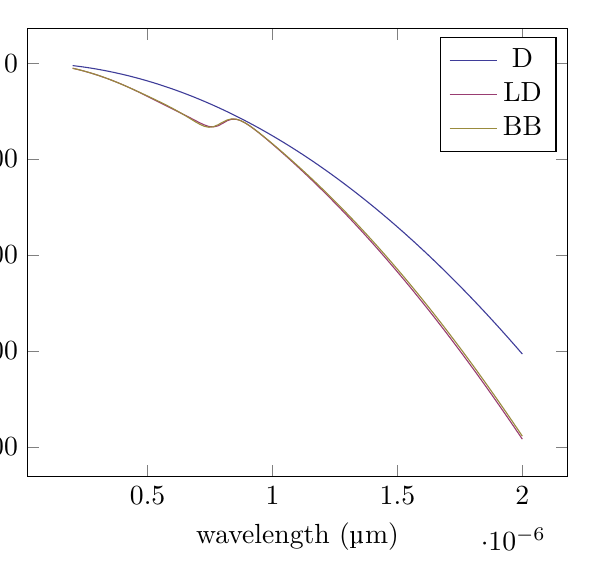
\begin{tikzpicture}[baseline,trim axis left]
\begin{axis}[xlabel=wavelength (\si{\micro\meter}),ylabel=$\epsilon'$]
\addplot[color=colora] coordinates {
(2e-07, -2.05370939621)
(2.18181818182e-07, -2.63412684958)
(2.36363636364e-07, -3.26500100129)
(2.54545454545e-07, -3.94632825579)
(2.72727272727e-07, -4.67810473015)
(2.90909090909e-07, -5.46032625407)
(3.09090909091e-07, -6.29298836996)
(3.27272727273e-07, -7.17608633302)
(3.45454545455e-07, -8.10961511128)
(3.63636363636e-07, -9.0935693857)
(3.81818181818e-07, -10.1279435502)
(4e-07, -11.2127317118)
(4.18181818182e-07, -12.3479276907)
(4.36363636364e-07, -13.5335250202)
(4.54545454545e-07, -14.7695169472)
(4.72727272727e-07, -16.0558964317)
(4.90909090909e-07, -17.3926561474)
(5.09090909091e-07, -18.7797884818)
(5.27272727273e-07, -20.2172855358)
(5.45454545455e-07, -21.7051391244)
(5.63636363636e-07, -23.2433407765)
(5.81818181818e-07, -24.8318817351)
(6e-07, -26.4707529574)
(6.18181818182e-07, -28.1599451149)
(6.36363636364e-07, -29.8994485937)
(6.54545454545e-07, -31.6892534944)
(6.72727272727e-07, -33.5293496324)
(6.90909090909e-07, -35.419726538)
(7.09090909091e-07, -37.3603734566)
(7.27272727273e-07, -39.3512793486)
(7.45454545455e-07, -41.3924328901)
(7.63636363636e-07, -43.4838224724)
(7.81818181818e-07, -45.6254362027)
(8e-07, -47.8172619039)
(8.18181818182e-07, -50.059287115)
(8.36363636364e-07, -52.3514990911)
(8.54545454545e-07, -54.693884804)
(8.72727272727e-07, -57.0864309416)
(8.90909090909e-07, -59.529123909)
(9.09090909091e-07, -62.0219498279)
(9.27272727273e-07, -64.5648945374)
(9.45454545455e-07, -67.1579435937)
(9.63636363636e-07, -69.8010822709)
(9.81818181818e-07, -72.4942955606)
(1e-06, -75.2375681723)
(1.01818181818e-06, -78.030884534)
(1.03636363636e-06, -80.8742287918)
(1.05454545455e-06, -83.7675848106)
(1.07272727273e-06, -86.7109361742)
(1.09090909091e-06, -89.7042661854)
(1.10909090909e-06, -92.7475578664)
(1.12727272727e-06, -95.8407939588)
(1.14545454545e-06, -98.9839569244)
(1.16363636364e-06, -102.177028945)
(1.18181818182e-06, -105.419991921)
(1.2e-06, -108.712827477)
(1.21818181818e-06, -112.055516956)
(1.23636363636e-06, -115.448041421)
(1.25454545455e-06, -118.890381659)
(1.27272727273e-06, -122.382518177)
(1.29090909091e-06, -125.924431205)
(1.30909090909e-06, -129.516100693)
(1.32727272727e-06, -133.157506317)
(1.34545454545e-06, -136.848627472)
(1.36363636364e-06, -140.589443279)
(1.38181818182e-06, -144.379932581)
(1.4e-06, -148.220073944)
(1.41818181818e-06, -152.10984566)
(1.43636363636e-06, -156.049225743)
(1.45454545455e-06, -160.038191933)
(1.47272727273e-06, -164.076721694)
(1.49090909091e-06, -168.164792216)
(1.50909090909e-06, -172.302380413)
(1.52727272727e-06, -176.489462928)
(1.54545454545e-06, -180.726016127)
(1.56363636364e-06, -185.012016103)
(1.58181818182e-06, -189.347438678)
(1.6e-06, -193.732259398)
(1.61818181818e-06, -198.166453539)
(1.63636363636e-06, -202.649996104)
(1.65454545455e-06, -207.182861823)
(1.67272727273e-06, -211.765025158)
(1.69090909091e-06, -216.396460295)
(1.70909090909e-06, -221.077141154)
(1.72727272727e-06, -225.807041382)
(1.74545454545e-06, -230.586134357)
(1.76363636364e-06, -235.414393186)
(1.78181818182e-06, -240.291790708)
(1.8e-06, -245.218299494)
(1.81818181818e-06, -250.193891844)
(1.83636363636e-06, -255.218539792)
(1.85454545455e-06, -260.292215104)
(1.87272727273e-06, -265.414889278)
(1.89090909091e-06, -270.586533546)
(1.90909090909e-06, -275.807118872)
(1.92727272727e-06, -281.076615956)
(1.94545454545e-06, -286.39499523)
(1.96363636364e-06, -291.762226862)
(1.98181818182e-06, -297.178280756)
(2e-06, -302.643126551)
};
\addlegendentry{D}
\addplot[color=colorb] coordinates {
(2e-07, -4.84561350949)
(2.18181818182e-07, -5.95573185139)
(2.36363636364e-07, -7.15856524757)
(2.54545454545e-07, -8.45183002905)
(2.72727272727e-07, -9.8332348867)
(2.90909090909e-07, -11.3010178159)
(3.09090909091e-07, -12.8544706742)
(3.27272727273e-07, -14.494165647)
(3.45454545455e-07, -16.221656534)
(3.63636363636e-07, -18.0386662639)
(3.81818181818e-07, -19.9460289403)
(4e-07, -21.9427325886)
(4.18181818182e-07, -24.0252815815)
(4.36363636364e-07, -26.1874112097)
(4.54545454545e-07, -28.420083404)
(4.72727272727e-07, -30.711701003)
(4.90909090909e-07, -33.0485460179)
(5.09090909091e-07, -35.4155139777)
(5.27272727273e-07, -37.7972428448)
(5.45454545455e-07, -40.1797002573)
(5.63636363636e-07, -42.5521851764)
(5.81818181818e-07, -44.9095181175)
(6e-07, -47.2539542292)
(6.18181818182e-07, -49.5960853957)
(6.36363636364e-07, -51.9537110876)
(6.54545454545e-07, -54.347271803)
(6.72727272727e-07, -56.789703239)
(6.90909090909e-07, -59.2671013072)
(7.09090909091e-07, -61.7044616929)
(7.27272727273e-07, -63.9111009625)
(7.45454545455e-07, -65.5171140581)
(7.63636363636e-07, -65.9785771106)
(7.81818181818e-07, -64.840961033)
(8e-07, -62.3264216409)
(8.18181818182e-07, -59.5976526348)
(8.36363636364e-07, -57.9707205456)
(8.54545454545e-07, -57.9865375628)
(8.72727272727e-07, -59.443903206)
(8.90909090909e-07, -61.9028545693)
(9.09090909091e-07, -64.9878844003)
(9.27272727273e-07, -68.4517090751)
(9.45454545455e-07, -72.1482445794)
(9.63636363636e-07, -75.9952423114)
(9.81818181818e-07, -79.9473849347)
(1e-06, -83.9799936574)
(1.01818181818e-06, -88.079782141)
(1.03636363636e-06, -92.2397325324)
(1.05454545455e-06, -96.4562721179)
(1.07272727273e-06, -100.727714455)
(1.09090909091e-06, -105.053394694)
(1.10909090909e-06, -109.433187983)
(1.12727272727e-06, -113.867240859)
(1.14545454545e-06, -118.355821971)
(1.16363636364e-06, -122.899240044)
(1.18181818182e-06, -127.497799911)
(1.2e-06, -132.151780048)
(1.21818181818e-06, -136.861422222)
(1.23636363636e-06, -141.626927851)
(1.25454545455e-06, -146.448457977)
(1.27272727273e-06, -151.326135112)
(1.29090909091e-06, -156.260045921)
(1.30909090909e-06, -161.250244215)
(1.32727272727e-06, -166.296753935)
(1.34545454545e-06, -171.399571979)
(1.36363636364e-06, -176.558670806)
(1.38181818182e-06, -181.774000788)
(1.4e-06, -187.045492322)
(1.41818181818e-06, -192.373057706)
(1.43636363636e-06, -197.756592816)
(1.45454545455e-06, -203.19597859)
(1.47272727273e-06, -208.691082354)
(1.49090909091e-06, -214.241758998)
(1.50909090909e-06, -219.847852039)
(1.52727272727e-06, -225.509194559)
(1.54545454545e-06, -231.225610066)
(1.56363636364e-06, -236.996913256)
(1.58181818182e-06, -242.822910714)
(1.6e-06, -248.703401546)
(1.61818181818e-06, -254.638177956)
(1.63636363636e-06, -260.627025776)
(1.65454545455e-06, -266.669724947)
(1.67272727273e-06, -272.76604997)
(1.69090909091e-06, -278.915770314)
(1.70909090909e-06, -285.118650799)
(1.72727272727e-06, -291.374451948)
(1.74545454545e-06, -297.682930319)
(1.76363636364e-06, -304.043838807)
(1.78181818182e-06, -310.456926932)
(1.8e-06, -316.92194111)
(1.81818181818e-06, -323.438624901)
(1.83636363636e-06, -330.006719247)
(1.85454545455e-06, -336.625962694)
(1.87272727273e-06, -343.296091604)
(1.89090909091e-06, -350.016840349)
(1.90909090909e-06, -356.787941504)
(1.92727272727e-06, -363.609126023)
(1.94545454545e-06, -370.480123407)
(1.96363636364e-06, -377.400661863)
(1.98181818182e-06, -384.370468461)
(2e-06, -391.389269277)
};
\addlegendentry{LD}
\addplot[color=colorc] coordinates {
(2e-07, -4.83284754023)
(2.18181818182e-07, -5.92655486136)
(2.36363636364e-07, -7.11387139167)
(2.54545454545e-07, -8.39659921977)
(2.72727272727e-07, -9.77572608492)
(2.90909090909e-07, -11.2512715733)
(3.09090909091e-07, -12.8222248683)
(3.27272727273e-07, -14.4864673824)
(3.45454545455e-07, -16.2406489403)
(3.63636363636e-07, -18.0800331452)
(3.81818181818e-07, -19.9983631074)
(4e-07, -21.9878315697)
(4.18181818182e-07, -24.0392634324)
(4.36363636364e-07, -26.1426142757)
(4.54545454545e-07, -28.2878360811)
(4.72727272727e-07, -30.4660623484)
(4.90909090909e-07, -32.670952749)
(5.09090909091e-07, -34.8999627195)
(5.27272727273e-07, -37.1553000283)
(5.45454545455e-07, -39.444392219)
(5.63636363636e-07, -41.7797717969)
(5.81818181818e-07, -44.178326698)
(6e-07, -46.6597919558)
(6.18181818182e-07, -49.2440860884)
(6.36363636364e-07, -51.9464740837)
(6.54545454545e-07, -54.7683099839)
(6.72727272727e-07, -57.6790051112)
(6.90909090909e-07, -60.582552076)
(7.09090909091e-07, -63.2648476284)
(7.27272727273e-07, -65.3432876535)
(7.45454545455e-07, -66.3034045707)
(7.63636363636e-07, -65.7406596728)
(7.81818181818e-07, -63.7476473618)
(8e-07, -61.0718807637)
(8.18181818182e-07, -58.7653864931)
(8.36363636364e-07, -57.6180768627)
(8.54545454545e-07, -57.882527224)
(8.72727272727e-07, -59.3920388404)
(8.90909090909e-07, -61.8175871946)
(9.09090909091e-07, -64.8482252253)
(9.27272727273e-07, -68.2565744016)
(9.45454545455e-07, -71.8973311191)
(9.63636363636e-07, -75.6847452208)
(9.81818181818e-07, -79.570797211)
(1e-06, -83.5297381225)
(1.01818181818e-06, -87.5484497375)
(1.03636363636e-06, -91.6207913308)
(1.05454545455e-06, -95.7443841921)
(1.07272727273e-06, -99.9188119583)
(1.09090909091e-06, -104.144624278)
(1.10909090909e-06, -108.422791898)
(1.12727272727e-06, -112.754414442)
(1.14545454545e-06, -117.140569259)
(1.16363636364e-06, -121.58223859)
(1.18181818182e-06, -126.080279722)
(1.2e-06, -130.635418187)
(1.21818181818e-06, -135.248252783)
(1.23636363636e-06, -139.919266132)
(1.25454545455e-06, -144.648837305)
(1.27272727273e-06, -149.43725467)
(1.29090909091e-06, -154.284728014)
(1.30909090909e-06, -159.191399518)
(1.32727272727e-06, -164.15735345)
(1.34545454545e-06, -169.182624593)
(1.36363636364e-06, -174.267205479)
(1.38181818182e-06, -179.411052581)
(1.4e-06, -184.614091568)
(1.41818181818e-06, -189.876221754)
(1.43636363636e-06, -195.197319874)
(1.45454545455e-06, -200.577243261)
(1.47272727273e-06, -206.015832544)
(1.49090909091e-06, -211.51291392)
(1.50909090909e-06, -217.068301081)
(1.52727272727e-06, -222.681796846)
(1.54545454545e-06, -228.353194543)
(1.56363636364e-06, -234.082279191)
(1.58181818182e-06, -239.868828498)
(1.6e-06, -245.712613718)
(1.61818181818e-06, -251.613400388)
(1.63636363636e-06, -257.570948951)
(1.65454545455e-06, -263.585015307)
(1.67272727273e-06, -269.655351274)
(1.69090909091e-06, -275.781705001)
(1.70909090909e-06, -281.963821318)
(1.72727272727e-06, -288.20144205)
(1.74545454545e-06, -294.494306291)
(1.76363636364e-06, -300.842150638)
(1.78181818182e-06, -307.244709414)
(1.8e-06, -313.701714853)
(1.81818181818e-06, -320.212897276)
(1.83636363636e-06, -326.777985242)
(1.85454545455e-06, -333.396705692)
(1.87272727273e-06, -340.068784077)
(1.89090909091e-06, -346.793944475)
(1.90909090909e-06, -353.571909701)
(1.92727272727e-06, -360.402401411)
(1.94545454545e-06, -367.285140193)
(1.96363636364e-06, -374.219845658)
(1.98181818182e-06, -381.206236528)
(2e-06, -388.244030709)
};
\addlegendentry{BB}
\end{axis}
\end{tikzpicture}%
\\
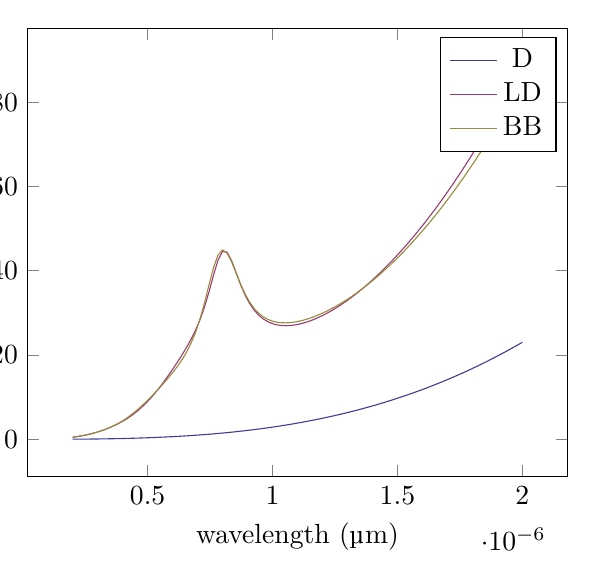
\begin{tikzpicture}[baseline,trim axis left]
\begin{axis}[xlabel=wavelength (\si{\micro\meter}),ylabel=$\epsilon''$]
\addplot[color=colora] coordinates {
(2e-07, 0.0231520386981)
(2.18181818182e-07, 0.0300573146374)
(2.36363636364e-07, 0.0382147778154)
(2.54545454545e-07, 0.0477287234718)
(2.72727272727e-07, 0.0587034339617)
(2.90909090909e-07, 0.0712431777668)
(3.09090909091e-07, 0.085452208505)
(3.27272727273e-07, 0.101434763942)
(3.45454545455e-07, 0.119295065)
(3.63636363636e-07, 0.139137314775)
(3.81818181818e-07, 0.161065697539)
(4e-07, 0.185184377762)
(4.18181818182e-07, 0.211597499118)
(4.36363636364e-07, 0.240409183501)
(4.54545454545e-07, 0.271723530036)
(4.72727272727e-07, 0.305644614096)
(4.90909090909e-07, 0.342276486313)
(5.09090909091e-07, 0.381723171595)
(5.27272727273e-07, 0.424088668141)
(5.45454545455e-07, 0.469476946455)
(5.63636363636e-07, 0.517991948365)
(5.81818181818e-07, 0.569737586038)
(6e-07, 0.624817740998)
(6.18181818182e-07, 0.683336263147)
(6.36363636364e-07, 0.745396969777)
(6.54545454545e-07, 0.811103644598)
(6.72727272727e-07, 0.880560036749)
(6.90909090909e-07, 0.953869859828)
(7.09090909091e-07, 1.03113679091)
(7.27272727273e-07, 1.11246446955)
(7.45454545455e-07, 1.19795649686)
(7.63636363636e-07, 1.28771643447)
(7.81818181818e-07, 1.38184780358)
(8e-07, 1.48045408399)
(8.18181818182e-07, 1.58363871313)
(8.36363636364e-07, 1.69150508506)
(8.54545454545e-07, 1.80415654953)
(8.72727272727e-07, 1.92169641098)
(8.90909090909e-07, 2.04422792761)
(9.09090909091e-07, 2.17185431036)
(9.27272727273e-07, 2.30467872197)
(9.45454545455e-07, 2.44280427602)
(9.63636363636e-07, 2.58633403594)
(9.81818181818e-07, 2.73537101405)
(1e-06, 2.89001817063)
(1.01818181818e-06, 3.0503784129)
(1.03636363636e-06, 3.2165545941)
(1.05454545455e-06, 3.38864951251)
(1.07272727273e-06, 3.5667659105)
(1.09090909091e-06, 3.75100647354)
(1.10909090909e-06, 3.9414738293)
(1.12727272727e-06, 4.13827054665)
(1.14545454545e-06, 4.34149913469)
(1.16363636364e-06, 4.55126204186)
(1.18181818182e-06, 4.76766165491)
(1.2e-06, 4.99080029799)
(1.21818181818e-06, 5.22078023172)
(1.23636363636e-06, 5.45770365217)
(1.25454545455e-06, 5.70167268999)
(1.27272727273e-06, 5.95278940942)
(1.29090909091e-06, 6.21115580733)
(1.30909090909e-06, 6.47687381231)
(1.32727272727e-06, 6.75004528374)
(1.34545454545e-06, 7.03077201077)
(1.36363636364e-06, 7.31915571148)
(1.38181818182e-06, 7.61529803186)
(1.4e-06, 7.91930054493)
(1.41818181818e-06, 8.23126474974)
(1.43636363636e-06, 8.55129207053)
(1.45454545455e-06, 8.87948385569)
(1.47272727273e-06, 9.21594137691)
(1.49090909091e-06, 9.5607658282)
(1.50909090909e-06, 9.91405832499)
(1.52727272727e-06, 10.2759199032)
(1.54545454545e-06, 10.6464515183)
(1.56363636364e-06, 11.0257540444)
(1.58181818182e-06, 11.4139282733)
(1.6e-06, 11.8110749135)
(1.61818181818e-06, 12.2172945897)
(1.63636363636e-06, 12.6326878412)
(1.65454545455e-06, 13.0573551214)
(1.67272727273e-06, 13.491396797)
(1.69090909091e-06, 13.9349131468)
(1.70909090909e-06, 14.3880043608)
(1.72727272727e-06, 14.8507705395)
(1.74545454545e-06, 15.323311693)
(1.76363636364e-06, 15.8057277398)
(1.78181818182e-06, 16.2981185061)
(1.8e-06, 16.8005837249)
(1.81818181818e-06, 17.3132230351)
(1.83636363636e-06, 17.8361359805)
(1.85454545455e-06, 18.3694220091)
(1.87272727273e-06, 18.9131804719)
(1.89090909091e-06, 19.4675106224)
(1.90909090909e-06, 20.0325116153)
(1.92727272727e-06, 20.6082825061)
(1.94545454545e-06, 21.1949222495)
(1.96363636364e-06, 21.7925296994)
(1.98181818182e-06, 22.4012036071)
(2e-06, 23.0210426213)
};
\addlegendentry{D}
\addplot[color=colorb] coordinates {
(2e-07, 0.474063639008)
(2.18181818182e-07, 0.627957273325)
(2.36363636364e-07, 0.813900498701)
(2.54545454545e-07, 1.03448612659)
(2.72727272727e-07, 1.29155260532)
(2.90909090909e-07, 1.58622790001)
(3.09090909091e-07, 1.91935564664)
(3.27272727273e-07, 2.29228008352)
(3.45454545455e-07, 2.70773925814)
(3.63636363636e-07, 3.17049635635)
(3.81818181818e-07, 3.68744858293)
(4e-07, 4.26720911582)
(4.18181818182e-07, 4.91935467397)
(4.36363636364e-07, 5.65355641801)
(4.54545454545e-07, 6.47871792826)
(4.72727272727e-07, 7.40214455897)
(4.90909090909e-07, 8.42873231798)
(5.09090909091e-07, 9.56019975699)
(5.27272727273e-07, 10.7944723405)
(5.45454545455e-07, 12.1254383984)
(5.63636363636e-07, 13.5433989138)
(5.81818181818e-07, 15.0365939962)
(6e-07, 16.5941709373)
(6.18181818182e-07, 18.2108442137)
(6.36363636364e-07, 19.8933010013)
(6.54545454545e-07, 21.6681423566)
(6.72727272727e-07, 23.5906874452)
(6.90909090909e-07, 25.7526372422)
(7.09090909091e-07, 28.282403923)
(7.27272727273e-07, 31.3206543091)
(7.45454545455e-07, 34.9319542649)
(7.63636363636e-07, 38.9040646177)
(7.81818181818e-07, 42.5017489163)
(8e-07, 44.5798842553)
(8.18181818182e-07, 44.4091611093)
(8.36363636364e-07, 42.3704472543)
(8.54545454545e-07, 39.4927857913)
(8.72727272727e-07, 36.6169424694)
(8.90909090909e-07, 34.135925062)
(9.09090909091e-07, 32.1398556545)
(9.27272727273e-07, 30.58922726)
(9.45454545455e-07, 29.4096144578)
(9.63636363636e-07, 28.5288910994)
(9.81818181818e-07, 27.8877160369)
(1e-06, 27.4401267846)
(1.01818181818e-06, 27.1512862508)
(1.03636363636e-06, 26.9948952753)
(1.05454545455e-06, 26.9510059793)
(1.07272727273e-06, 27.0043496523)
(1.09090909091e-06, 27.1431083361)
(1.10909090909e-06, 27.3580258817)
(1.12727272727e-06, 27.6417664729)
(1.14545454545e-06, 27.9884499863)
(1.16363636364e-06, 28.3933129366)
(1.18181818182e-06, 28.8524587113)
(1.2e-06, 29.3626716244)
(1.21818181818e-06, 29.9212769388)
(1.23636363636e-06, 30.5260342989)
(1.25454545455e-06, 31.1750556894)
(1.27272727273e-06, 31.8667415822)
(1.29090909091e-06, 32.599730713)
(1.30909090909e-06, 33.3728601769)
(1.32727272727e-06, 34.1851334165)
(1.34545454545e-06, 35.0356943077)
(1.36363636364e-06, 35.9238059994)
(1.38181818182e-06, 36.8488334962)
(1.4e-06, 37.8102292145)
(1.41818181818e-06, 38.8075209173)
(1.43636363636e-06, 39.8403015717)
(1.45454545455e-06, 40.9082207697)
(1.47272727273e-06, 42.0109774299)
(1.49090909091e-06, 43.1483135549)
(1.50909090909e-06, 44.3200088677)
(1.52727272727e-06, 45.52587618)
(1.54545454545e-06, 46.7657573761)
(1.56363636364e-06, 48.0395199169)
(1.58181818182e-06, 49.3470537862)
(1.6e-06, 50.688268812)
(1.61818181818e-06, 52.0630923114)
(1.63636363636e-06, 53.4714670129)
(1.65454545455e-06, 54.9133492176)
(1.67272727273e-06, 56.3887071697)
(1.69090909091e-06, 57.8975196061)
(1.70909090909e-06, 59.4397744652)
(1.72727272727e-06, 61.0154677334)
(1.74545454545e-06, 62.6246024131)
(1.76363636364e-06, 64.2671875976)
(1.78181818182e-06, 65.9432376408)
(1.8e-06, 67.6527714103)
(1.81818181818e-06, 69.3958116149)
(1.83636363636e-06, 71.1723841989)
(1.85454545455e-06, 72.9825177938)
(1.87272727273e-06, 74.8262432249)
(1.89090909091e-06, 76.7035930631)
(1.90909090909e-06, 78.6146012207)
(1.92727272727e-06, 80.5593025847)
(1.94545454545e-06, 82.537732684)
(1.96363636364e-06, 84.5499273887)
(1.98181818182e-06, 86.5959226367)
(2e-06, 88.6757541862)
};
\addlegendentry{LD}
\addplot[color=colorc] coordinates {
(2e-07, 0.508748362656)
(2.18181818182e-07, 0.663033304698)
(2.36363636364e-07, 0.841682585377)
(2.54545454545e-07, 1.04840143644)
(2.72727272727e-07, 1.28799479441)
(2.90909090909e-07, 1.56599256697)
(3.09090909091e-07, 1.88840820147)
(3.27272727273e-07, 2.26156915875)
(3.45454545455e-07, 2.69194325728)
(3.63636363636e-07, 3.18589404419)
(3.81818181818e-07, 3.74931477505)
(4e-07, 4.38711876394)
(4.18181818182e-07, 5.10261341575)
(4.36363636364e-07, 5.89685624422)
(4.54545454545e-07, 6.76816293007)
(4.72727272727e-07, 7.71197265335)
(4.90909090909e-07, 8.72124466367)
(5.09090909091e-07, 9.78746662652)
(5.27272727273e-07, 10.9022420799)
(5.45454545455e-07, 12.0593481239)
(5.63636363636e-07, 13.2571557416)
(5.81818181818e-07, 14.5013928923)
(6e-07, 15.8083853436)
(6.18181818182e-07, 17.2090873886)
(6.36363636364e-07, 18.7543091841)
(6.54545454545e-07, 20.5212439938)
(6.72727272727e-07, 22.6197384883)
(6.90909090909e-07, 25.1912684001)
(7.09090909091e-07, 28.3803567475)
(7.27272727273e-07, 32.2408307074)
(7.45454545455e-07, 36.5582558671)
(7.63636363636e-07, 40.6966414167)
(7.81818181818e-07, 43.7268359445)
(8e-07, 44.9178011895)
(8.18181818182e-07, 44.1933200073)
(8.36363636364e-07, 42.1053565427)
(8.54545454545e-07, 39.4197024723)
(8.72727272727e-07, 36.7413842563)
(8.90909090909e-07, 34.3950723446)
(9.09090909091e-07, 32.4850625248)
(9.27272727273e-07, 30.9966775012)
(9.45454545455e-07, 29.8701258589)
(9.63636363636e-07, 29.0386709839)
(9.81818181818e-07, 28.4435693425)
(1e-06, 28.0376941846)
(1.01818181818e-06, 27.7847474722)
(1.03636363636e-06, 27.6572319211)
(1.05454545455e-06, 27.6344042328)
(1.07272727273e-06, 27.7005775961)
(1.09090909091e-06, 27.8438172768)
(1.10909090909e-06, 28.0549712558)
(1.12727272727e-06, 28.3269597535)
(1.14545454545e-06, 28.6542564406)
(1.16363636364e-06, 29.0325089348)
(1.18181818182e-06, 29.4582598221)
(1.2e-06, 29.9287402062)
(1.21818181818e-06, 30.4417157618)
(1.23636363636e-06, 30.9953710059)
(1.25454545455e-06, 31.5882215722)
(1.27272727273e-06, 32.219047155)
(1.29090909091e-06, 32.8868398251)
(1.30909090909e-06, 33.5907638659)
(1.32727272727e-06, 34.3301243097)
(1.34545454545e-06, 35.104342094)
(1.36363636364e-06, 35.9129342927)
(1.38181818182e-06, 36.7554982653)
(1.4e-06, 37.6316988537)
(1.41818181818e-06, 38.5412579645)
(1.43636363636e-06, 39.483946033)
(1.45454545455e-06, 40.4595749793)
(1.47272727273e-06, 41.467992357)
(1.49090909091e-06, 42.5090764605)
(1.50909090909e-06, 43.5827322074)
(1.52727272727e-06, 44.6888876518)
(1.54545454545e-06, 45.8274910144)
(1.56363636364e-06, 46.9985081377)
(1.58181818182e-06, 48.2019202933)
(1.6e-06, 49.4377222836)
(1.61818181818e-06, 50.7059207888)
(1.63636363636e-06, 52.0065329205)
(1.65454545455e-06, 53.3395849516)
(1.67272727273e-06, 54.7051111947)
(1.69090909091e-06, 56.1031530083)
(1.70909090909e-06, 57.5337579127)
(1.72727272727e-06, 58.9969788009)
(1.74545454545e-06, 60.4928732308)
(1.76363636364e-06, 62.0215027901)
(1.78181818182e-06, 63.5829325232)
(1.8e-06, 65.1772304135)
(1.81818181818e-06, 66.8044669138)
(1.83636363636e-06, 68.4647145203)
(1.85454545455e-06, 70.1580473845)
(1.87272727273e-06, 71.8845409594)
(1.89090909091e-06, 73.644271676)
(1.90909090909e-06, 75.4373166473)
(1.92727272727e-06, 77.2637533969)
(1.94545454545e-06, 79.1236596103)
(1.96363636364e-06, 81.0171129054)
(1.98181818182e-06, 82.9441906227)
(2e-06, 84.9049696306)
};
\addlegendentry{BB}
\end{axis}
\end{tikzpicture}%
\\
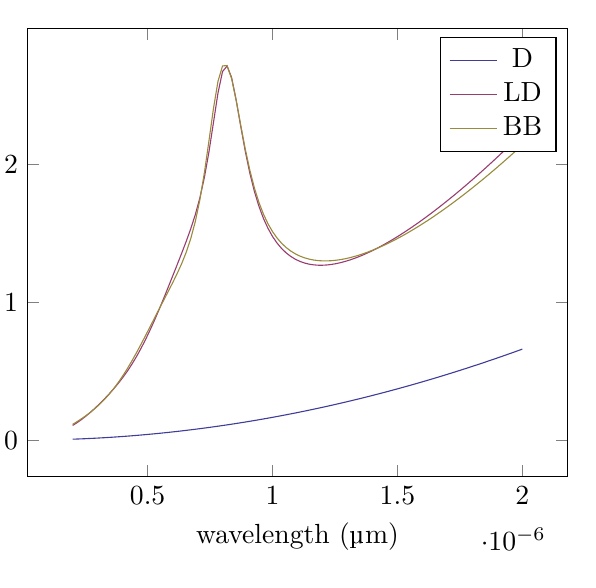
\begin{tikzpicture}[baseline,trim axis left]
\begin{axis}[xlabel=wavelength (\si{\micro\meter}),ylabel=$n'$]
\addplot[color=colora] coordinates {
(2e-07, 0.00807760942817)
(2.18181818182e-07, 0.0092596542616)
(2.36363636364e-07, 0.0105743150928)
(2.54545454545e-07, 0.01201282857)
(2.72727272727e-07, 0.0135703170118)
(2.90909090909e-07, 0.0152438529201)
(3.09090909091e-07, 0.0170315754235)
(3.27272727273e-07, 0.0189322466557)
(3.45454545455e-07, 0.020945012059)
(3.63636363636e-07, 0.0230692630717)
(3.81818181818e-07, 0.0253045546188)
(4e-07, 0.0276505535182)
(4.18181818182e-07, 0.0301070051121)
(4.36363636364e-07, 0.0326737110507)
(4.54545454545e-07, 0.0353505141246)
(4.72727272727e-07, 0.0381372876774)
(4.90909090909e-07, 0.0410339280707)
(5.09090909091e-07, 0.0440403492264)
(5.27272727273e-07, 0.0471564786118)
(5.45454545455e-07, 0.0503822542436)
(5.63636363636e-07, 0.0537176224245)
(5.81818181818e-07, 0.0571625360116)
(6e-07, 0.0607169530786)
(6.18181818182e-07, 0.0643808358718)
(6.36363636364e-07, 0.0681541499874)
(6.54545454545e-07, 0.0720368637186)
(6.72727272727e-07, 0.0760289475322)
(6.90909090909e-07, 0.0801303736476)
(7.09090909091e-07, 0.0843411156939)
(7.27272727273e-07, 0.088661148431)
(7.45454545455e-07, 0.093090447519)
(7.63636363636e-07, 0.0976289893286)
(7.81818181818e-07, 0.102276750784)
(8e-07, 0.107033709229)
(8.18181818182e-07, 0.111899842319)
(8.36363636364e-07, 0.116875127928)
(8.54545454545e-07, 0.121959544066)
(8.72727272727e-07, 0.127153068817)
(8.90909090909e-07, 0.132455680277)
(9.09090909091e-07, 0.137867356511)
(9.27272727273e-07, 0.143388075506)
(9.45454545455e-07, 0.149017815137)
(9.63636363636e-07, 0.154756553134)
(9.81818181818e-07, 0.160604267061)
(1e-06, 0.166560934283)
(1.01818181818e-06, 0.172626531952)
(1.03636363636e-06, 0.178801036991)
(1.05454545455e-06, 0.18508442607)
(1.07272727273e-06, 0.1914766756)
(1.09090909091e-06, 0.197977761719)
(1.10909090909e-06, 0.204587660279)
(1.12727272727e-06, 0.211306346839)
(1.14545454545e-06, 0.218133796656)
(1.16363636364e-06, 0.225069984677)
(1.18181818182e-06, 0.232114885535)
(1.2e-06, 0.239268473539)
(1.21818181818e-06, 0.246530722674)
(1.23636363636e-06, 0.253901606592)
(1.25454545455e-06, 0.261381098609)
(1.27272727273e-06, 0.268969171704)
(1.29090909091e-06, 0.276665798513)
(1.30909090909e-06, 0.284470951328)
(1.32727272727e-06, 0.292384602091)
(1.34545454545e-06, 0.300406722396)
(1.36363636364e-06, 0.308537283486)
(1.38181818182e-06, 0.316776256249)
(1.4e-06, 0.325123611217)
(1.41818181818e-06, 0.333579318567)
(1.43636363636e-06, 0.342143348117)
(1.45454545455e-06, 0.350815669327)
(1.47272727273e-06, 0.359596251295)
(1.49090909091e-06, 0.368485062761)
(1.50909090909e-06, 0.377482072099)
(1.52727272727e-06, 0.386587247325)
(1.54545454545e-06, 0.395800556089)
(1.56363636364e-06, 0.40512196568)
(1.58181818182e-06, 0.414551443019)
(1.6e-06, 0.424088954668)
(1.61818181818e-06, 0.433734466821)
(1.63636363636e-06, 0.443487945307)
(1.65454545455e-06, 0.453349355592)
(1.67272727273e-06, 0.463318662776)
(1.69090909091e-06, 0.473395831592)
(1.70909090909e-06, 0.48358082641)
(1.72727272727e-06, 0.493873611235)
(1.74545454545e-06, 0.504274149704)
(1.76363636364e-06, 0.514782405091)
(1.78181818182e-06, 0.525398340303)
(1.8e-06, 0.536121917884)
(1.81818181818e-06, 0.546953100012)
(1.83636363636e-06, 0.557891848499)
(1.85454545455e-06, 0.568938124793)
(1.87272727273e-06, 0.58009188998)
(1.89090909091e-06, 0.591353104777)
(1.90909090909e-06, 0.602721729542)
(1.92727272727e-06, 0.614197724265)
(1.94545454545e-06, 0.625781048574)
(1.96363636364e-06, 0.637471661736)
(1.98181818182e-06, 0.649269522651)
(2e-06, 0.661174589859)
};
\addlegendentry{D}
\addplot[color=colorb] coordinates {
(2e-07, 0.10755101629)
(2.18181818182e-07, 0.12847881497)
(2.36363636364e-07, 0.151855298031)
(2.54545454545e-07, 0.177586744258)
(2.72727272727e-07, 0.205495994117)
(2.90909090909e-07, 0.235350487146)
(3.09090909091e-07, 0.266930404659)
(3.27272727273e-07, 0.3001206052)
(3.45454545455e-07, 0.334990299912)
(3.63636363636e-07, 0.371823748491)
(3.81818181818e-07, 0.411088862723)
(4e-07, 0.453360876084)
(4.18181818182e-07, 0.499232513289)
(4.36363636364e-07, 0.549235215071)
(4.54545454545e-07, 0.603779999557)
(4.72727272727e-07, 0.663114658352)
(4.90909090909e-07, 0.72729081081)
(5.09090909091e-07, 0.79613782039)
(5.27272727273e-07, 0.86924714147)
(5.45454545455e-07, 0.945977744643)
(5.63636363636e-07, 1.02549922597)
(5.81818181818e-07, 1.10689261297)
(6e-07, 1.18932837016)
(6.18181818182e-07, 1.27233600147)
(6.36363636364e-07, 1.35617064399)
(6.54545454545e-07, 1.4422701235)
(6.72727272727e-07, 1.53377609505)
(6.90909090909e-07, 1.6360368465)
(7.09090909091e-07, 1.75682820375)
(7.27272727273e-07, 1.90552006442)
(7.45454545455e-07, 2.08933859392)
(7.63636363636e-07, 2.30388821387)
(7.81818181818e-07, 2.5187356572)
(8e-07, 2.67415606058)
(8.18181818182e-07, 2.71351487301)
(8.36363636364e-07, 2.62998018898)
(8.54545454545e-07, 2.46690849363)
(8.72727272727e-07, 2.27737166294)
(8.90909090909e-07, 2.09621051933)
(9.09090909091e-07, 1.93818454094)
(9.27272727273e-07, 1.80608263189)
(9.45454545455e-07, 1.69762346786)
(9.63636363636e-07, 1.60911278818)
(9.81818181818e-07, 1.53694300431)
(1e-06, 1.47805826457)
(1.01818181818e-06, 1.43000805657)
(1.03636363636e-06, 1.39086693109)
(1.05454545455e-06, 1.35912840675)
(1.07272727273e-06, 1.33360925378)
(1.09090909091e-06, 1.31337273591)
(1.10909090909e-06, 1.29766993357)
(1.12727272727e-06, 1.28589575538)
(1.14545454545e-06, 1.27755614742)
(1.16363636364e-06, 1.2722436077)
(1.18181818182e-06, 1.26961879538)
(1.2e-06, 1.26939660494)
(1.21818181818e-06, 1.27133552261)
(1.23636363636e-06, 1.27522941062)
(1.25454545455e-06, 1.28090110177)
(1.27272727273e-06, 1.28819735618)
(1.29090909091e-06, 1.29698485239)
(1.30909090909e-06, 1.30714697166)
(1.32727272727e-06, 1.3185811962)
(1.34545454545e-06, 1.33119698697)
(1.36363636364e-06, 1.34491403954)
(1.38181818182e-06, 1.3596608403)
(1.4e-06, 1.37537346363)
(1.41818181818e-06, 1.39199456337)
(1.43636363636e-06, 1.40947252253)
(1.45454545455e-06, 1.42776073253)
(1.47272727273e-06, 1.44681697914)
(1.49090909091e-06, 1.46660291698)
(1.50909090909e-06, 1.48708361784)
(1.52727272727e-06, 1.5082271808)
(1.54545454545e-06, 1.53000439455)
(1.56363636364e-06, 1.55238844372)
(1.58181818182e-06, 1.57535465281)
(1.6e-06, 1.59888026202)
(1.61818181818e-06, 1.62294423057)
(1.63636363636e-06, 1.64752706351)
(1.65454545455e-06, 1.67261065899)
(1.67272727273e-06, 1.69817817305)
(1.69090909091e-06, 1.72421389974)
(1.70909090909e-06, 1.75070316455)
(1.72727272727e-06, 1.77763222948)
(1.74545454545e-06, 1.80498820831)
(1.76363636364e-06, 1.83275899078)
(1.78181818182e-06, 1.86093317471)
(1.8e-06, 1.88950000493)
(1.81818181818e-06, 1.91844931854)
(1.83636363636e-06, 1.94777149539)
(1.85454545455e-06, 1.9774574136)
(1.87272727273e-06, 2.00749840918)
(1.89090909091e-06, 2.03788623962)
(1.90909090909e-06, 2.06861305082)
(1.92727272727e-06, 2.09967134708)
(1.94545454545e-06, 2.13105396386)
(1.96363636364e-06, 2.16275404296)
(1.98181818182e-06, 2.1947650099)
(2e-06, 2.22708055333)
};
\addlegendentry{LD}
\addplot[color=colorc] coordinates {
(2e-07, 0.115550647905)
(2.18181818182e-07, 0.135965243961)
(2.36363636364e-07, 0.157510445654)
(2.54545454545e-07, 0.180552900373)
(2.72727272727e-07, 0.205529090078)
(2.90909090909e-07, 0.232870677799)
(3.09090909091e-07, 0.26297602463)
(3.27272727273e-07, 0.296201649784)
(3.45454545455e-07, 0.332857131156)
(3.63636363636e-07, 0.373194642787)
(3.81818181818e-07, 0.417389210337)
(4e-07, 0.465509551329)
(4.18181818182e-07, 0.517483516041)
(4.36363636364e-07, 0.573066746988)
(4.54545454545e-07, 0.63182663859)
(4.72727272727e-07, 0.693153698654)
(4.90909090909e-07, 0.756307952892)
(5.09090909091e-07, 0.820500649109)
(5.27272727273e-07, 0.885004659145)
(5.45454545455e-07, 0.949283894558)
(5.63636363636e-07, 1.01313416382)
(5.81818181818e-07, 1.07683465936)
(6e-07, 1.14131903292)
(6.18181818182e-07, 1.2083855596)
(6.36363636364e-07, 1.28097269966)
(6.54545454545e-07, 1.36351542172)
(6.72727272727e-07, 1.46232472314)
(6.90909090909e-07, 1.58568128377)
(7.09090909091e-07, 1.74270919794)
(7.27272727273e-07, 1.939211474)
(7.45454545455e-07, 2.16919854033)
(7.63636363636e-07, 2.40595064126)
(7.81818181818e-07, 2.60342497131)
(8e-07, 2.71473929837)
(8.18181818182e-07, 2.71688945541)
(8.36363636364e-07, 2.62155542935)
(8.54545454545e-07, 2.46456686036)
(8.72727272727e-07, 2.28538204596)
(8.90909090909e-07, 2.11239730896)
(9.09090909091e-07, 1.95979243844)
(9.27272727273e-07, 1.831453504)
(9.45454545455e-07, 1.72597617641)
(9.63636363636e-07, 1.64005815911)
(9.81818181818e-07, 1.57018605346)
(1e-06, 1.51327787063)
(1.01818181818e-06, 1.46683117517)
(1.03636363636e-06, 1.4288803548)
(1.05454545455e-06, 1.39790012148)
(1.07272727273e-06, 1.37270824627)
(1.09090909091e-06, 1.35238393745)
(1.10909090909e-06, 1.33620413689)
(1.12727272727e-06, 1.32359538017)
(1.14545454545e-06, 1.31409791024)
(1.16363636364e-06, 1.3073390286)
(1.18181818182e-06, 1.30301327412)
(1.2e-06, 1.30086760934)
(1.21818181818e-06, 1.30069027485)
(1.23636363636e-06, 1.30230233799)
(1.25454545455e-06, 1.30555123019)
(1.27272727273e-06, 1.31030576159)
(1.29090909091e-06, 1.31645224079)
(1.30909090909e-06, 1.32389142783)
(1.32727272727e-06, 1.33253612015)
(1.34545454545e-06, 1.34230922361)
(1.36363636364e-06, 1.35314219776)
(1.38181818182e-06, 1.3649737926)
(1.4e-06, 1.37774901395)
(1.41818181818e-06, 1.39141826949)
(1.43636363636e-06, 1.40593665884)
(1.45454545455e-06, 1.42126337908)
(1.47272727273e-06, 1.4373612238)
(1.49090909091e-06, 1.45419615815)
(1.50909090909e-06, 1.47173695615)
(1.52727272727e-06, 1.4899548896)
(1.54545454545e-06, 1.50882345953)
(1.56363636364e-06, 1.52831816345)
(1.58181818182e-06, 1.54841629254)
(1.6e-06, 1.56909675422)
(1.61818181818e-06, 1.59033991624)
(1.63636363636e-06, 1.61212746912)
(1.65454545455e-06, 1.6344423045)
(1.67272727273e-06, 1.65726840692)
(1.69090909091e-06, 1.68059075757)
(1.70909090909e-06, 1.70439524815)
(1.72727272727e-06, 1.72866860373)
(1.74545454545e-06, 1.75339831345)
(1.76363636364e-06, 1.77857256808)
(1.78181818182e-06, 1.80418020372)
(1.8e-06, 1.83021065077)
(1.81818181818e-06, 1.85665388776)
(1.83636363636e-06, 1.88350039943)
(1.85454545455e-06, 1.9107411385)
(1.87272727273e-06, 1.93836749095)
(1.89090909091e-06, 1.96637124424)
(1.90909090909e-06, 1.99474455833)
(1.92727272727e-06, 2.0234799391)
(1.94545454545e-06, 2.05257021399)
(1.96363636364e-06, 2.0820085097)
(1.98181818182e-06, 2.11178823161)
(2e-06, 2.14190304494)
};
\addlegendentry{BB}
\end{axis}
\end{tikzpicture}%
\\
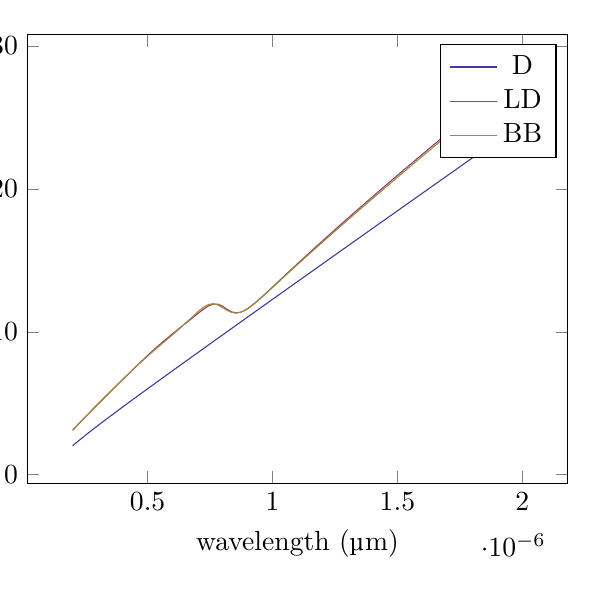
\begin{tikzpicture}[baseline,trim axis left]
\begin{axis}[xlabel=wavelength (\si{\micro\meter}),ylabel=$n''$]
\addplot[color=colora] coordinates {
(2e-07, 2.02670897959)
(2.18181818182e-07, 2.29530503018)
(2.36363636364e-07, 2.55543061633)
(2.54545454545e-07, 2.80943857874)
(2.72727272727e-07, 3.05885236115)
(2.90909090909e-07, 3.30471137291)
(3.09090909091e-07, 3.54775378078)
(3.27272727273e-07, 3.78852075697)
(3.45454545455e-07, 4.02741947277)
(3.63636363636e-07, 4.26476296565)
(3.81818181818e-07, 4.50079634525)
(4e-07, 4.73571457437)
(4.18181818182e-07, 4.9696748631)
(4.36363636364e-07, 5.2028055108)
(4.54545454545e-07, 5.43521234286)
(4.72727272727e-07, 5.66698348054)
(4.90909090909e-07, 5.89819293185)
(5.09090909091e-07, 6.12890333325)
(5.27272727273e-07, 6.35916806969)
(5.45454545455e-07, 6.58903293298)
(5.63636363636e-07, 6.81853743254)
(5.81818181818e-07, 7.04771584141)
(6e-07, 7.27659803834)
(6.18181818182e-07, 7.50521019118)
(6.36363636364e-07, 7.7335753157)
(6.54545454545e-07, 7.96171373563)
(6.72727272727e-07, 8.18964346394)
(6.90909090909e-07, 8.41738052066)
(7.09090909091e-07, 8.64493919936)
(7.27272727273e-07, 8.87233229178)
(7.45454545455e-07, 9.09957127798)
(7.63636363636e-07, 9.3266664883)
(7.81818181818e-07, 9.55362724168)
(8e-07, 9.78046196443)
(8.18181818182e-07, 10.0071782926)
(8.36363636364e-07, 10.2337831604)
(8.54545454545e-07, 10.4602828771)
(8.72727272727e-07, 10.686683194)
(8.90909090909e-07, 10.9129893628)
(9.09090909091e-07, 11.1392061868)
(9.27272727273e-07, 11.365338066)
(9.45454545455e-07, 11.591389037)
(9.63636363636e-07, 11.8173628075)
(9.81818181818e-07, 12.0432627881)
(1e-06, 12.2690921194)
(1.01818181818e-06, 12.4948536969)
(1.03636363636e-06, 12.7205501927)
(1.05454545455e-06, 12.9461840753)
(1.07272727273e-06, 13.1717576269)
(1.09090909091e-06, 13.3972729598)
(1.10909090909e-06, 13.6227320297)
(1.12727272727e-06, 13.8481366495)
(1.14545454545e-06, 14.0734884998)
(1.16363636364e-06, 14.2987891405)
(1.18181818182e-06, 14.5240400193)
(1.2e-06, 14.7492424809)
(1.21818181818e-06, 14.9743977744)
(1.23636363636e-06, 15.1995070609)
(1.25454545455e-06, 15.4245714195)
(1.27272727273e-06, 15.6495918536)
(1.29090909091e-06, 15.8745692961)
(1.30909090909e-06, 16.0995046144)
(1.32727272727e-06, 16.3243986151)
(1.34545454545e-06, 16.5492520478)
(1.36363636364e-06, 16.7740656094)
(1.38181818182e-06, 16.9988399473)
(1.4e-06, 17.2235756628)
(1.41818181818e-06, 17.4482733141)
(1.43636363636e-06, 17.6729334189)
(1.45454545455e-06, 17.897556457)
(1.47272727273e-06, 18.1221428732)
(1.49090909091e-06, 18.3466930784)
(1.50909090909e-06, 18.5712074528)
(1.52727272727e-06, 18.795686347)
(1.54545454545e-06, 19.0201300841)
(1.56363636364e-06, 19.244538961)
(1.58181818182e-06, 19.4689132504)
(1.6e-06, 19.693253202)
(1.61818181818e-06, 19.9175590436)
(1.63636363636e-06, 20.1418309824)
(1.65454545455e-06, 20.3660692065)
(1.67272727273e-06, 20.5902738855)
(1.69090909091e-06, 20.814445172)
(1.70909090909e-06, 21.0385832018)
(1.72727272727e-06, 21.2626880956)
(1.74545454545e-06, 21.4867599593)
(1.76363636364e-06, 21.7107988849)
(1.78181818182e-06, 21.9348049512)
(1.8e-06, 22.1587782247)
(1.81818181818e-06, 22.3827187597)
(1.83636363636e-06, 22.6066265996)
(1.85454545455e-06, 22.830501777)
(1.87272727273e-06, 23.0543443142)
(1.89090909091e-06, 23.2781542241)
(1.90909090909e-06, 23.5019315102)
(1.92727272727e-06, 23.7256761674)
(1.94545454545e-06, 23.9493881822)
(1.96363636364e-06, 24.1730675332)
(1.98181818182e-06, 24.3967141914)
(2e-06, 24.6203281208)
};
\addlegendentry{D}
\addplot[color=colorb] coordinates {
(2e-07, 3.11678704136)
(2.18181818182e-07, 3.4560783143)
(2.36363636364e-07, 3.78988793478)
(2.54545454545e-07, 4.11906957474)
(2.72727272727e-07, 4.4442015009)
(2.90909090909e-07, 4.76579640096)
(3.09090909091e-07, 5.08443163296)
(3.27272727273e-07, 5.40078476236)
(3.45454545455e-07, 5.71557084376)
(3.63636363636e-07, 6.02941442661)
(3.81818181818e-07, 6.34271597872)
(4e-07, 6.65556438967)
(4.18181818182e-07, 6.96771335286)
(4.36363636364e-07, 7.27860845645)
(4.54545454545e-07, 7.58744142539)
(4.72727272727e-07, 7.89321506778)
(4.90909090909e-07, 8.19481518295)
(5.09090909091e-07, 8.49109526583)
(5.27272727273e-07, 8.7809832522)
(5.45454545455e-07, 9.06361673403)
(5.63636363636e-07, 9.33850457396)
(5.81818181818e-07, 9.60569928471)
(6e-07, 9.86594711128)
(6.18181818182e-07, 10.1207632416)
(6.36363636364e-07, 10.3723584496)
(6.54545454545e-07, 10.6233153876)
(6.72727272727e-07, 10.8758606417)
(6.90909090909e-07, 11.1304732936)
(7.09090909091e-07, 11.3834008126)
(7.27272727273e-07, 11.6225735255)
(7.45454545455e-07, 11.8222205882)
(7.63636363636e-07, 11.9403917869)
(7.81818181818e-07, 11.9318892338)
(8e-07, 11.7879202811)
(8.18181818182e-07, 11.5724513912)
(8.36363636364e-07, 11.3918845096)
(8.54545454545e-07, 11.3200861374)
(8.72727272727e-07, 11.3692853687)
(8.90909090909e-07, 11.5149427363)
(9.09090909091e-07, 11.7255655484)
(9.27272727273e-07, 11.9761131882)
(9.45454545455e-07, 12.2499118379)
(9.63636363636e-07, 12.5367050118)
(9.81818181818e-07, 12.8303997391)
(1e-06, 13.1274254819)
(1.01818181818e-06, 13.425699623)
(1.03636363636e-06, 13.7240113198)
(1.05454545455e-06, 14.021661966)
(1.07272727273e-06, 14.3182560458)
(1.09090909091e-06, 14.6135787977)
(1.10909090909e-06, 14.9075239553)
(1.12727272727e-06, 15.2000505758)
(1.14545454545e-06, 15.4911569407)
(1.16363636364e-06, 15.7808646051)
(1.18181818182e-06, 16.0692085553)
(1.2e-06, 16.3562310933)
(1.21818181818e-06, 16.6419780215)
(1.23636363636e-06, 16.9264962647)
(1.25454545455e-06, 17.2098323995)
(1.27272727273e-06, 17.4920317597)
(1.29090909091e-06, 17.7731379125)
(1.30909090909e-06, 18.0531923726)
(1.32727272727e-06, 18.3322344686)
(1.34545454545e-06, 18.6103013085)
(1.36363636364e-06, 18.8874278069)
(1.38181818182e-06, 19.1636467505)
(1.4e-06, 19.4389888876)
(1.41818181818e-06, 19.7134830291)
(1.43636363636e-06, 19.9871561563)
(1.45454545455e-06, 20.2600335291)
(1.47272727273e-06, 20.5321387938)
(1.49090909091e-06, 20.803494087)
(1.50909090909e-06, 21.0741201347)
(1.52727272727e-06, 21.3440363469)
(1.54545454545e-06, 21.6132609068)
(1.56363636364e-06, 21.8818108545)
(1.58181818182e-06, 22.1497021649)
(1.6e-06, 22.416949821)
(1.61818181818e-06, 22.6835678821)
(1.63636363636e-06, 22.9495695472)
(1.65454545455e-06, 23.2149672136)
(1.67272727273e-06, 23.479772532)
(1.69090909091e-06, 23.7439964574)
(1.70909090909e-06, 24.0076492964)
(1.72727272727e-06, 24.2707407506)
(1.74545454545e-06, 24.5332799581)
(1.76363636364e-06, 24.7952755308)
(1.78181818182e-06, 25.05673559)
(1.8e-06, 25.3176677985)
(1.81818181818e-06, 25.5780793919)
(1.83636363636e-06, 25.8379772059)
(1.85454545455e-06, 26.0973677032)
(1.87272727273e-06, 26.3562569978)
(1.89090909091e-06, 26.6146508778)
(1.90909090909e-06, 26.8725548268)
(1.92727272727e-06, 27.1299740431)
(1.94545454545e-06, 27.3869134589)
(1.96363636364e-06, 27.6433777572)
(1.98181818182e-06, 27.8993713875)
(2e-06, 28.1548985815)
};
\addlegendentry{LD}
\addplot[color=colorc] coordinates {
(2e-07, 3.1132617919)
(2.18181818182e-07, 3.44819993879)
(2.36363636364e-07, 3.77853964705)
(2.54545454545e-07, 4.10589784812)
(2.72727272727e-07, 4.43124548898)
(2.90909090909e-07, 4.75510259108)
(3.09090909091e-07, 5.07767294296)
(3.27272727273e-07, 5.39892633766)
(3.45454545455e-07, 5.7186436871)
(3.63636363636e-07, 6.0364405715)
(3.81818181818e-07, 6.35178350706)
(4e-07, 6.66401241176)
(4.18181818182e-07, 6.97238160484)
(4.36363636364e-07, 7.27612805992)
(4.54545454545e-07, 7.57456810416)
(4.72727272727e-07, 7.86721353446)
(4.90909090909e-07, 8.15388919089)
(5.09090909091e-07, 8.43483064853)
(5.27272727273e-07, 8.71074431664)
(5.45454545455e-07, 8.98282050711)
(5.63636363636e-07, 9.25269826924)
(5.81818181818e-07, 9.52238411131)
(6e-07, 9.79412079676)
(6.18181818182e-07, 10.0701819)
(6.36363636364e-07, 10.3525228945)
(6.54545454545e-07, 10.6421317685)
(6.72727272727e-07, 10.937769307)
(6.90909090909e-07, 11.2336046939)
(7.09090909091e-07, 11.5153708561)
(7.27272727273e-07, 11.7561752959)
(7.45454545455e-07, 11.9171159999)
(7.63636363636e-07, 11.9607071832)
(7.81818181818e-07, 11.8764867653)
(8e-07, 11.6997171096)
(8.18181818182e-07, 11.5019019998)
(8.36363636364e-07, 11.3569916555)
(8.54545454545e-07, 11.3098733002)
(8.72727272727e-07, 11.367938242)
(8.90909090909e-07, 11.5134538333)
(9.09090909091e-07, 11.7208371397)
(9.27272727273e-07, 11.9675224118)
(9.45454545455e-07, 12.2373465164)
(9.63636363636e-07, 12.5199469636)
(9.81818181818e-07, 12.8090812671)
(1e-06, 13.1011257559)
(1.01818181818e-06, 13.394031763)
(1.03636363636e-06, 13.6866716479)
(1.05454545455e-06, 13.978448336)
(1.07272727273e-06, 14.2690672356)
(1.09090909091e-06, 14.5584042115)
(1.10909090909e-06, 14.8464294289)
(1.12727272727e-06, 15.1331635273)
(1.14545454545e-06, 15.4186525077)
(1.16363636364e-06, 15.7029534754)
(1.18181818182e-06, 15.9861266925)
(1.2e-06, 16.2682312944)
(1.21818181818e-06, 16.5493231266)
(1.23636363636e-06, 16.8294537945)
(1.25454545455e-06, 17.1086703937)
(1.27272727273e-06, 17.387015607)
(1.29090909091e-06, 17.6645279878)
(1.30909090909e-06, 17.9412423221)
(1.32727272727e-06, 18.2171900117)
(1.34545454545e-06, 18.4923994465)
(1.36363636364e-06, 18.7668963489)
(1.38181818182e-06, 19.0407040855)
(1.4e-06, 19.3138439423)
(1.41818181818e-06, 19.586335367)
(1.43636363636e-06, 19.8581961801)
(1.45454545455e-06, 20.129442757)
(1.47272727273e-06, 20.4000901877)
(1.49090909091e-06, 20.6701524129)
(1.50909090909e-06, 20.9396423441)
(1.52727272727e-06, 21.208571966)
(1.54545454545e-06, 21.476952427)
(1.56363636364e-06, 21.7447941172)
(1.58181818182e-06, 22.0121067376)
(1.6e-06, 22.2788993598)
(1.61818181818e-06, 22.54518048)
(1.63636363636e-06, 22.8109580653)
(1.65454545455e-06, 23.0762395963)
(1.67272727273e-06, 23.3410321043)
(1.69090909091e-06, 23.6053422045)
(1.70909090909e-06, 23.8691761265)
(1.72727272727e-06, 24.1325397417)
(1.74545454545e-06, 24.3954385874)
(1.76363636364e-06, 24.6578778899)
(1.78181818182e-06, 24.9198625847)
(1.8e-06, 25.1813973353)
(1.81818181818e-06, 25.4424865504)
(1.83636363636e-06, 25.7031344002)
(1.85454545455e-06, 25.9633448304)
(1.87272727273e-06, 26.2231215765)
(1.89090909091e-06, 26.4824681759)
(1.90909090909e-06, 26.7413879802)
(1.92727272727e-06, 26.9998841655)
(1.94545454545e-06, 27.257959743)
(1.96363636364e-06, 27.5156175687)
(1.98181818182e-06, 27.7728603519)
(2e-06, 28.0296906641)
};
\addlegendentry{BB}
\end{axis}
\end{tikzpicture}%
\\
\end{tabular}
\caption{Material parameters for Al based on the Drude, Lorentz-Drude, and Brendel-Bormann models.}
\end{figure}
\clearpage
\newpage
\subsection{Au}
\begin{figure}[h!]
\centering
\begin{tabular}{l}
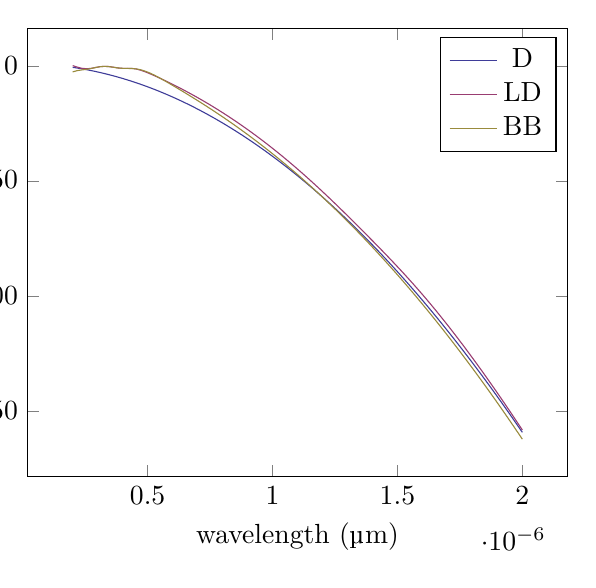
\begin{tikzpicture}[baseline,trim axis left]
\begin{axis}[xlabel=wavelength (\si{\micro\meter}),ylabel=$\epsilon'$]
\addplot[color=colora] coordinates {
(2e-07, -0.612444230451)
(2.18181818182e-07, -0.918915234983)
(2.36363636364e-07, -1.25202623397)
(2.54545454545e-07, -1.6117748134)
(2.72727272727e-07, -1.99815836634)
(2.90909090909e-07, -2.41117409299)
(3.09090909091e-07, -2.85081900072)
(3.27272727273e-07, -3.31708990416)
(3.45454545455e-07, -3.8099834252)
(3.63636363636e-07, -4.32949599312)
(3.81818181818e-07, -4.8756238446)
(4e-07, -5.4483630238)
(4.18181818182e-07, -6.04770938245)
(4.36363636364e-07, -6.67365857992)
(4.54545454545e-07, -7.32620608328)
(4.72727272727e-07, -8.00534716739)
(4.90909090909e-07, -8.71107691502)
(5.09090909091e-07, -9.44339021686)
(5.27272727273e-07, -10.2022817717)
(5.45454545455e-07, -10.9877460865)
(5.63636363636e-07, -11.7997774764)
(5.81818181818e-07, -12.6383700651)
(6e-07, -13.5035177844)
(6.18181818182e-07, -14.395214375)
(6.36363636364e-07, -15.3134533862)
(6.54545454545e-07, -16.2582281761)
(6.72727272727e-07, -17.2295319116)
(6.90909090909e-07, -18.2273575689)
(7.09090909091e-07, -19.2516979332)
(7.27272727273e-07, -20.302545599)
(7.45454545455e-07, -21.3798929702)
(7.63636363636e-07, -22.4837322606)
(7.81818181818e-07, -23.6140554932)
(8e-07, -24.7708545013)
(8.18181818182e-07, -25.954120928)
(8.36363636364e-07, -27.1638462267)
(8.54545454545e-07, -28.4000216608)
(8.72727272727e-07, -29.6626383045)
(8.90909090909e-07, -30.9516870426)
(9.09090909091e-07, -32.2671585705)
(9.27272727273e-07, -33.6090433946)
(9.45454545455e-07, -34.9773318327)
(9.63636363636e-07, -36.3720140136)
(9.81818181818e-07, -37.7930798777)
(1e-06, -39.2405191771)
(1.01818181818e-06, -40.7143214757)
(1.03636363636e-06, -42.2144761495)
(1.05454545455e-06, -43.7409723866)
(1.07272727273e-06, -45.2937991877)
(1.09090909091e-06, -46.872945366)
(1.10909090909e-06, -48.4783995475)
(1.12727272727e-06, -50.1101501714)
(1.14545454545e-06, -51.7681854899)
(1.16363636364e-06, -53.4524935688)
(1.18181818182e-06, -55.1630622876)
(1.2e-06, -56.8998793394)
(1.21818181818e-06, -58.6629322318)
(1.23636363636e-06, -60.4522082865)
(1.25454545455e-06, -62.2676946396)
(1.27272727273e-06, -64.1093782423)
(1.29090909091e-06, -65.9772458605)
(1.30909090909e-06, -67.8712840757)
(1.32727272727e-06, -69.7914792846)
(1.34545454545e-06, -71.7378176997)
(1.36363636364e-06, -73.7102853494)
(1.38181818182e-06, -75.7088680787)
(1.4e-06, -77.7335515486)
(1.41818181818e-06, -79.7843212371)
(1.43636363636e-06, -81.8611624391)
(1.45454545455e-06, -83.9640602669)
(1.47272727273e-06, -86.0929996502)
(1.49090909091e-06, -88.2479653365)
(1.50909090909e-06, -90.4289418914)
(1.52727272727e-06, -92.6359136987)
(1.54545454545e-06, -94.8688649612)
(1.56363636364e-06, -97.1277797001)
(1.58181818182e-06, -99.4126417561)
(1.6e-06, -101.723434789)
(1.61818181818e-06, -104.06014228)
(1.63636363636e-06, -106.422747527)
(1.65454545455e-06, -108.811233651)
(1.67272727273e-06, -111.225583594)
(1.69090909091e-06, -113.665780116)
(1.70909090909e-06, -116.131805802)
(1.72727272727e-06, -118.623643055)
(1.74545454545e-06, -121.141274103)
(1.76363636364e-06, -123.684680993)
(1.78181818182e-06, -126.253845598)
(1.8e-06, -128.848749612)
(1.81818181818e-06, -131.469374551)
(1.83636363636e-06, -134.115701756)
(1.85454545455e-06, -136.787712392)
(1.87272727273e-06, -139.485387448)
(1.89090909091e-06, -142.208707737)
(1.90909090909e-06, -144.957653897)
(1.92727272727e-06, -147.73220639)
(1.94545454545e-06, -150.532345506)
(1.96363636364e-06, -153.358051359)
(1.98181818182e-06, -156.209303889)
(2e-06, -159.086082864)
};
\addlegendentry{D}
\addplot[color=colorb] coordinates {
(2e-07, 0.137249454114)
(2.18181818182e-07, -0.524999663898)
(2.36363636364e-07, -1.02404097811)
(2.54545454545e-07, -1.23421163137)
(2.72727272727e-07, -1.09097977687)
(2.90909090909e-07, -0.708186463362)
(3.09090909091e-07, -0.338333849862)
(3.27272727273e-07, -0.182619469914)
(3.45454545455e-07, -0.287625118735)
(3.63636363636e-07, -0.576294468847)
(3.81818181818e-07, -0.893991602649)
(4e-07, -1.06116342422)
(4.18181818182e-07, -1.04182427031)
(4.36363636364e-07, -1.06292884396)
(4.54545454545e-07, -1.34162753759)
(4.72727272727e-07, -1.87929488229)
(4.90909090909e-07, -2.58560857276)
(5.09090909091e-07, -3.38809381579)
(5.27272727273e-07, -4.2468882114)
(5.45454545455e-07, -5.14276754502)
(5.63636363636e-07, -6.06701247566)
(5.81818181818e-07, -7.01590995807)
(6e-07, -7.98808580079)
(6.18181818182e-07, -8.98324487532)
(6.36363636364e-07, -10.0015757735)
(6.54545454545e-07, -11.0434677346)
(6.72727272727e-07, -12.1093760433)
(6.90909090909e-07, -13.1997590707)
(7.09090909091e-07, -14.315050272)
(7.27272727273e-07, -15.4556472799)
(7.45454545455e-07, -16.6219092445)
(7.63636363636e-07, -17.8141579797)
(7.81818181818e-07, -19.0326806713)
(8e-07, -20.2777330177)
(8.18181818182e-07, -21.5495422381)
(8.36363636364e-07, -22.8483096764)
(8.54545454545e-07, -24.1742128704)
(8.72727272727e-07, -25.5274070259)
(8.90909090909e-07, -26.9080258646)
(9.09090909091e-07, -28.3161818177)
(9.27272727273e-07, -29.7519655358)
(9.45454545455e-07, -31.2154446698)
(9.63636363636e-07, -32.7066618636)
(9.81818181818e-07, -34.2256318835)
(1e-06, -35.7723377929)
(1.01818181818e-06, -37.3467260656)
(1.03636363636e-06, -38.9487005262)
(1.05454545455e-06, -40.5781150053)
(1.07272727273e-06, -42.2347646176)
(1.09090909091e-06, -43.9183756073)
(1.10909090909e-06, -45.6285937884)
(1.12727272727e-06, -47.3649717283)
(1.14545454545e-06, -49.12695502)
(1.16363636364e-06, -50.9138682712)
(1.18181818182e-06, -52.7249018267)
(1.2e-06, -54.5591007516)
(1.21818181818e-06, -56.4153582288)
(1.23636363636e-06, -58.2924162319)
(1.25454545455e-06, -60.188877028)
(1.27272727273e-06, -62.1032295946)
(1.29090909091e-06, -64.0338951222)
(1.30909090909e-06, -65.9792951032)
(1.32727272727e-06, -67.9379436824)
(1.34545454545e-06, -69.9085626868)
(1.36363636364e-06, -71.8902130449)
(1.38181818182e-06, -73.8824306355)
(1.4e-06, -75.8853491328)
(1.41818181818e-06, -77.8997888853)
(1.43636363636e-06, -79.9272912171)
(1.45454545455e-06, -81.9700830765)
(1.47272727273e-06, -84.0309675391)
(1.49090909091e-06, -86.1131491988)
(1.50909090909e-06, -88.2200163562)
(1.52727272727e-06, -90.3549102653)
(1.54545454545e-06, -92.5209130302)
(1.56363636364e-06, -94.7206799499)
(1.58181818182e-06, -96.9563314507)
(1.6e-06, -99.2294076836)
(1.61818181818e-06, -101.540878656)
(1.63636363636e-06, -103.891196343)
(1.65454545455e-06, -106.280372973)
(1.67272727273e-06, -108.708070761)
(1.69090909091e-06, -111.173691454)
(1.70909090909e-06, -113.67645783)
(1.72727272727e-06, -116.215482819)
(1.74545454545e-06, -118.789824715)
(1.76363636364e-06, -121.398528854)
(1.78181818182e-06, -124.040657259)
(1.8e-06, -126.715308257)
(1.81818181818e-06, -129.421628142)
(1.83636363636e-06, -132.158816843)
(1.85454545455e-06, -134.926129218)
(1.87272727273e-06, -137.722873358)
(1.89090909091e-06, -140.548406914)
(1.90909090909e-06, -143.402132243)
(1.92727272727e-06, -146.283490947)
(1.94545454545e-06, -149.191958188)
(1.96363636364e-06, -152.12703706)
(1.98181818182e-06, -155.088253175)
(2e-06, -158.075149584)
};
\addlegendentry{LD}
\addplot[color=colorc] coordinates {
(2e-07, -2.60791298748)
(2.18181818182e-07, -2.05123761556)
(2.36363636364e-07, -1.74747424378)
(2.54545454545e-07, -1.50301127078)
(2.72727272727e-07, -1.15271381876)
(2.90909090909e-07, -0.721233912431)
(3.09090909091e-07, -0.352653765359)
(3.27272727273e-07, -0.196533496093)
(3.45454545455e-07, -0.310635417437)
(3.63636363636e-07, -0.603867391749)
(3.81818181818e-07, -0.893512122806)
(4e-07, -1.05122265167)
(4.18181818182e-07, -1.09128318182)
(4.36363636364e-07, -1.13314154833)
(4.54545454545e-07, -1.30713500546)
(4.72727272727e-07, -1.68991639806)
(4.90909090909e-07, -2.29368510447)
(5.09090909091e-07, -3.08752426906)
(5.27272727273e-07, -4.02402542199)
(5.45454545455e-07, -5.05762821406)
(5.63636363636e-07, -6.15287282157)
(5.81818181818e-07, -7.28577130855)
(6e-07, -8.44191677355)
(6.18181818182e-07, -9.61372567165)
(6.36363636364e-07, -10.7979632525)
(6.54545454545e-07, -11.9939113148)
(6.72727272727e-07, -13.2021592637)
(6.90909090909e-07, -14.4238731878)
(7.09090909091e-07, -15.6603870808)
(7.27272727273e-07, -16.9129950322)
(7.45454545455e-07, -18.1828596143)
(7.63636363636e-07, -19.4709835461)
(7.81818181818e-07, -20.7782126624)
(8e-07, -22.1052526999)
(8.18181818182e-07, -23.4526903974)
(8.36363636364e-07, -24.8210143258)
(8.54545454545e-07, -26.2106334628)
(8.72727272727e-07, -27.6218928915)
(8.90909090909e-07, -29.0550866557)
(9.09090909091e-07, -30.5104680847)
(9.27272727273e-07, -31.9882579838)
(9.45454545455e-07, -33.4886510817)
(9.63636363636e-07, -35.0118210836)
(9.81818181818e-07, -36.557924619)
(1e-06, -38.1271043247)
(1.01818181818e-06, -39.7194912511)
(1.03636363636e-06, -41.3352067416)
(1.05454545455e-06, -42.9743639041)
(1.07272727273e-06, -44.6370687643)
(1.09090909091e-06, -46.3234211731)
(1.10909090909e-06, -48.0335155238)
(1.12727272727e-06, -49.7674413205)
(1.14545454545e-06, -51.525283633)
(1.16363636364e-06, -53.3071234626)
(1.18181818182e-06, -55.1130380388)
(1.2e-06, -56.9431010641)
(1.21818181818e-06, -58.7973829165)
(1.23636363636e-06, -60.6759508214)
(1.25454545455e-06, -62.578868998)
(1.27272727273e-06, -64.5061987876)
(1.29090909091e-06, -66.4579987668)
(1.30909090909e-06, -68.4343248493)
(1.32727272727e-06, -70.4352303792)
(1.34545454545e-06, -72.4607662172)
(1.36363636364e-06, -74.510980821)
(1.38181818182e-06, -76.5859203224)
(1.4e-06, -78.6856285993)
(1.41818181818e-06, -80.8101473462)
(1.43636363636e-06, -82.9595161418)
(1.45454545455e-06, -85.1337725137)
(1.47272727273e-06, -87.3329520025)
(1.49090909091e-06, -89.557088223)
(1.50909090909e-06, -91.8062129247)
(1.52727272727e-06, -94.0803560498)
(1.54545454545e-06, -96.3795457904)
(1.56363636364e-06, -98.7038086442)
(1.58181818182e-06, -101.053169468)
(1.6e-06, -103.427651532)
(1.61818181818e-06, -105.827276567)
(1.63636363636e-06, -108.252064819)
(1.65454545455e-06, -110.702035094)
(1.67272727273e-06, -113.177204807)
(1.69090909091e-06, -115.677590026)
(1.70909090909e-06, -118.203205517)
(1.72727272727e-06, -120.754064784)
(1.74545454545e-06, -123.330180115)
(1.76363636364e-06, -125.931562619)
(1.78181818182e-06, -128.558222263)
(1.8e-06, -131.210167914)
(1.81818181818e-06, -133.887407368)
(1.83636363636e-06, -136.589947392)
(1.85454545455e-06, -139.317793754)
(1.87272727273e-06, -142.070951254)
(1.89090909091e-06, -144.849423756)
(1.90909090909e-06, -147.653214221)
(1.92727272727e-06, -150.482324731)
(1.94545454545e-06, -153.336756519)
(1.96363636364e-06, -156.216509996)
(1.98181818182e-06, -159.121584778)
(2e-06, -162.051979705)
};
\addlegendentry{BB}
\end{axis}
\end{tikzpicture}%
\\
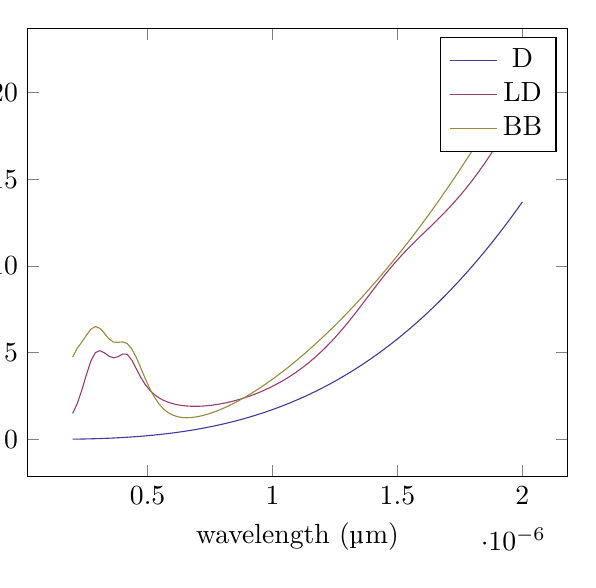
\begin{tikzpicture}[baseline,trim axis left]
\begin{axis}[xlabel=wavelength (\si{\micro\meter}),ylabel=$\epsilon''$]
\addplot[color=colora] coordinates {
(2e-07, 0.0137855547875)
(2.18181818182e-07, 0.017897150812)
(2.36363636364e-07, 0.022754309366)
(2.54545454545e-07, 0.0284191200053)
(2.72727272727e-07, 0.0349536625319)
(2.90909090909e-07, 0.0424200062447)
(3.09090909091e-07, 0.0508802091905)
(3.27272727273e-07, 0.0603963174156)
(3.45454545455e-07, 0.0710303642175)
(3.63636363636e-07, 0.082844369397)
(3.81818181818e-07, 0.0959003385104)
(4e-07, 0.110260262123)
(4.18181818182e-07, 0.125986115061)
(4.36363636364e-07, 0.143139855665)
(4.54545454545e-07, 0.161783425048)
(4.72727272727e-07, 0.181978746343)
(4.90909090909e-07, 0.203787723963)
(5.09090909091e-07, 0.227272242854)
(5.27272727273e-07, 0.252494167752)
(5.45454545455e-07, 0.279515342439)
(5.63636363636e-07, 0.308397588999)
(5.81818181818e-07, 0.339202707078)
(6e-07, 0.371992473138)
(6.18181818182e-07, 0.406828639719)
(6.36363636364e-07, 0.443772934696)
(6.54545454545e-07, 0.48288706054)
(6.72727272727e-07, 0.52423269358)
(6.90909090909e-07, 0.567871483259)
(7.09090909091e-07, 0.613865051401)
(7.27272727273e-07, 0.662274991471)
(7.45454545455e-07, 0.71316286784)
(7.63636363636e-07, 0.766590215045)
(7.81818181818e-07, 0.822618537058)
(8e-07, 0.881309306551)
(8.18181818182e-07, 0.942723964158)
(8.36363636364e-07, 1.00692391775)
(8.54545454545e-07, 1.07397054169)
(8.72727272727e-07, 1.14392517611)
(8.90909090909e-07, 1.2168491262)
(9.09090909091e-07, 1.29280366143)
(9.27272727273e-07, 1.37185001487)
(9.45454545455e-07, 1.45404938244)
(9.63636363636e-07, 1.53946292216)
(9.81818181818e-07, 1.6281517535)
(1e-06, 1.72017695656)
(1.01818181818e-06, 1.81559957141)
(1.03636363636e-06, 1.91448059735)
(1.05454545455e-06, 2.01688099217)
(1.07272727273e-06, 2.12286167147)
(1.09090909091e-06, 2.2324835079)
(1.10909090909e-06, 2.34580733046)
(1.12727272727e-06, 2.46289392378)
(1.14545454545e-06, 2.5838040274)
(1.16363636364e-06, 2.70859833508)
(1.18181818182e-06, 2.83733749402)
(1.2e-06, 2.97008210423)
(1.21818181818e-06, 3.10689271776)
(1.23636363636e-06, 3.24782983802)
(1.25454545455e-06, 3.39295391904)
(1.27272727273e-06, 3.54232536481)
(1.29090909091e-06, 3.69600452852)
(1.30909090909e-06, 3.85405171188)
(1.32727272727e-06, 4.01652716442)
(1.34545454545e-06, 4.18349108279)
(1.36363636364e-06, 4.35500361002)
(1.38181818182e-06, 4.5311248349)
(1.4e-06, 4.71191479116)
(1.41818181818e-06, 4.89743345691)
(1.43636363636e-06, 5.08774075383)
(1.45454545455e-06, 5.28289654654)
(1.47272727273e-06, 5.48296064189)
(1.49090909091e-06, 5.68799278825)
(1.50909090909e-06, 5.89805267485)
(1.52727272727e-06, 6.11319993107)
(1.54545454545e-06, 6.33349412575)
(1.56363636364e-06, 6.55899476654)
(1.58181818182e-06, 6.78976129915)
(1.6e-06, 7.02585310673)
(1.61818181818e-06, 7.26732950916)
(1.63636363636e-06, 7.51424976236)
(1.65454545455e-06, 7.76667305765)
(1.67272727273e-06, 8.02465852101)
(1.69090909091e-06, 8.28826521248)
(1.70909090909e-06, 8.55755212543)
(1.72727272727e-06, 8.83257818592)
(1.74545454545e-06, 9.113402252)
(1.76363636364e-06, 9.40008311308)
(1.78181818182e-06, 9.69267948922)
(1.8e-06, 9.99125003051)
(1.81818181818e-06, 10.2958533164)
(1.83636363636e-06, 10.6065478549)
(1.85454545455e-06, 10.9233920822)
(1.87272727273e-06, 11.2464443618)
(1.89090909091e-06, 11.5757629839)
(1.90909090909e-06, 11.9114061648)
(1.92727272727e-06, 12.253432046)
(1.94545454545e-06, 12.6018986941)
(1.96363636364e-06, 12.9568640994)
(1.98181818182e-06, 13.318386176)
(2e-06, 13.6865227607)
};
\addlegendentry{D}
\addplot[color=colorb] coordinates {
(2e-07, 1.49564119267)
(2.18181818182e-07, 2.06275498531)
(2.36363636364e-07, 2.82735261106)
(2.54545454545e-07, 3.70897197255)
(2.72727272727e-07, 4.50901475333)
(2.90909090909e-07, 5.00241916206)
(3.09090909091e-07, 5.1197498043)
(3.27272727273e-07, 4.9872504314)
(3.45454545455e-07, 4.7983168851)
(3.63636363636e-07, 4.70482396792)
(3.81818181818e-07, 4.77233578941)
(4e-07, 4.92068749355)
(4.18181818182e-07, 4.90884775231)
(4.36363636364e-07, 4.58361071469)
(4.54545454545e-07, 4.07461851599)
(4.72727272727e-07, 3.57125381732)
(4.90909090909e-07, 3.1549583407)
(5.09090909091e-07, 2.83194150505)
(5.27272727273e-07, 2.58553172119)
(5.45454545455e-07, 2.39771840201)
(5.63636363636e-07, 2.25428933624)
(5.81818181818e-07, 2.14492436739)
(6e-07, 2.06227635875)
(6.18181818182e-07, 2.00109890934)
(6.36363636364e-07, 1.95760288027)
(6.54545454545e-07, 1.92901404421)
(6.72727272727e-07, 1.91327445657)
(6.90909090909e-07, 1.90884042651)
(7.09090909091e-07, 1.91454438348)
(7.27272727273e-07, 1.92949910511)
(7.45454545455e-07, 1.95303032815)
(7.63636363636e-07, 1.98462865121)
(7.81818181818e-07, 2.0239147613)
(8e-07, 2.07061401546)
(8.18181818182e-07, 2.12453770059)
(8.36363636364e-07, 2.18556913815)
(8.54545454545e-07, 2.2536533591)
(8.72727272727e-07, 2.32878944803)
(8.90909090909e-07, 2.41102490822)
(9.09090909091e-07, 2.50045157049)
(9.27272727273e-07, 2.5972026843)
(9.45454545455e-07, 2.70145090519)
(9.63636363636e-07, 2.81340693862)
(9.81818181818e-07, 2.93331862303)
(1e-06, 3.06147023707)
(1.01818181818e-06, 3.19818179997)
(1.03636363636e-06, 3.34380809931)
(1.05454545455e-06, 3.49873712634)
(1.07272727273e-06, 3.66338752589)
(1.09090909091e-06, 3.83820457357)
(1.10909090909e-06, 4.02365408096)
(1.12727272727e-06, 4.22021350361)
(1.14545454545e-06, 4.42835939816)
(1.16363636364e-06, 4.64855026516)
(1.18181818182e-06, 4.88120375608)
(1.2e-06, 5.12666726946)
(1.21818181818e-06, 5.38518118607)
(1.23636363636e-06, 5.65683448941)
(1.25454545455e-06, 5.94151339353)
(1.27272727273e-06, 6.23884494831)
(1.29090909091e-06, 6.54813945196)
(1.30909090909e-06, 6.86833778802)
(1.32727272727e-06, 7.19797222836)
(1.34545454545e-06, 7.53515124343)
(1.36363636364e-06, 7.877579599)
(1.38181818182e-06, 8.22262351982)
(1.4e-06, 8.56742617653)
(1.41818181818e-06, 8.90907107192)
(1.43636363636e-06, 9.24478105457)
(1.45454545455e-06, 9.57213091167)
(1.47272727273e-06, 9.88924482529)
(1.49090909091e-06, 10.1949491661)
(1.50909090909e-06, 10.4888573198)
(1.52727272727e-06, 10.7713752835)
(1.54545454545e-06, 11.0436313109)
(1.56363636364e-06, 11.3073457714)
(1.58181818182e-06, 11.5646653367)
(1.6e-06, 11.8179873044)
(1.61818181818e-06, 12.0697961502)
(1.63636363636e-06, 12.3225274337)
(1.65454545455e-06, 12.5784664277)
(1.67272727273e-06, 12.8396821766)
(1.69090909091e-06, 13.1079930728)
(1.70909090909e-06, 13.3849576056)
(1.72727272727e-06, 13.6718832803)
(1.74545454545e-06, 13.9698472373)
(1.76363636364e-06, 14.2797232456)
(1.78181818182e-06, 14.6022110782)
(1.8e-06, 14.9378655254)
(1.81818181818e-06, 15.2871233453)
(1.83636363636e-06, 15.6503272337)
(1.85454545455e-06, 16.0277464554)
(1.87272727273e-06, 16.4195941364)
(1.89090909091e-06, 16.826041433)
(1.90909090909e-06, 17.247228902)
(1.92727272727e-06, 17.6832754387)
(1.94545454545e-06, 18.1342851457)
(1.96363636364e-06, 18.6003524688)
(1.98181818182e-06, 19.0815659)
(2e-06, 19.5780105011)
};
\addlegendentry{LD}
\addplot[color=colorc] coordinates {
(2e-07, 4.74384464474)
(2.18181818182e-07, 5.25255421461)
(2.36363636364e-07, 5.60183470209)
(2.54545454545e-07, 5.99650579411)
(2.72727272727e-07, 6.34982228603)
(2.90909090909e-07, 6.50598374719)
(3.09090909091e-07, 6.40283059357)
(3.27272727273e-07, 6.10913239381)
(3.45454545455e-07, 5.79126330887)
(3.63636363636e-07, 5.60991367549)
(3.81818181818e-07, 5.59387650798)
(4e-07, 5.62092656562)
(4.18181818182e-07, 5.52712588864)
(4.36363636364e-07, 5.22337958255)
(4.54545454545e-07, 4.72666055925)
(4.72727272727e-07, 4.1194713518)
(4.90909090909e-07, 3.49472447858)
(5.09090909091e-07, 2.92176500416)
(5.27272727273e-07, 2.43759543046)
(5.45454545455e-07, 2.05283359582)
(5.63636363636e-07, 1.76191905286)
(5.81818181818e-07, 1.55188224644)
(6e-07, 1.40801993612)
(6.18181818182e-07, 1.31683192847)
(6.36363636364e-07, 1.26714150868)
(6.54545454545e-07, 1.25022557324)
(6.72727272727e-07, 1.25950715855)
(6.90909090909e-07, 1.29011944662)
(7.09090909091e-07, 1.33848739032)
(7.27272727273e-07, 1.40198099572)
(7.45454545455e-07, 1.47864906053)
(7.63636363636e-07, 1.56702364216)
(7.81818181818e-07, 1.66598031989)
(8e-07, 1.77463994595)
(8.18181818182e-07, 1.89230016396)
(8.36363636364e-07, 2.01838782453)
(8.54545454545e-07, 2.15242587953)
(8.72727272727e-07, 2.29401023699)
(8.90909090909e-07, 2.44279344952)
(9.09090909091e-07, 2.59847309287)
(9.27272727273e-07, 2.76078337345)
(9.45454545455e-07, 2.92948897004)
(9.63636363636e-07, 3.1043804319)
(9.81818181818e-07, 3.28527067031)
(1e-06, 3.47199222591)
(1.01818181818e-06, 3.6643950927)
(1.03636363636e-06, 3.86234494687)
(1.05454545455e-06, 4.06572167417)
(1.07272727273e-06, 4.27441812127)
(1.09090909091e-06, 4.48833901806)
(1.10909090909e-06, 4.70740003303)
(1.12727272727e-06, 4.93152693434)
(1.14545454545e-06, 5.16065483658)
(1.16363636364e-06, 5.39472751855)
(1.18181818182e-06, 5.63369680077)
(1.2e-06, 5.87752197459)
(1.21818181818e-06, 6.1261692761)
(1.23636363636e-06, 6.37961139993)
(1.25454545455e-06, 6.63782704868)
(1.27272727273e-06, 6.90080051461)
(1.29090909091e-06, 7.16852129083)
(1.30909090909e-06, 7.44098370945)
(1.32727272727e-06, 7.71818660465)
(1.34545454545e-06, 8.00013299889)
(1.36363636364e-06, 8.28682981044)
(1.38181818182e-06, 8.57828758082)
(1.4e-06, 8.87452022081)
(1.41818181818e-06, 9.17554477372)
(1.43636363636e-06, 9.48138119473)
(1.45454545455e-06, 9.7920521453)
(1.47272727273e-06, 10.1075828016)
(1.49090909091e-06, 10.4280006759)
(1.50909090909e-06, 10.7533354504)
(1.52727272727e-06, 11.0836188222)
(1.54545454545e-06, 11.4188843592)
(1.56363636364e-06, 11.7591673653)
(1.58181818182e-06, 12.1045047555)
(1.6e-06, 12.4549349394)
(1.61818181818e-06, 12.8104977123)
(1.63636363636e-06, 13.1712341544)
(1.65454545455e-06, 13.5371865365)
(1.67272727273e-06, 13.9083982323)
(1.69090909091e-06, 14.2849136368)
(1.70909090909e-06, 14.6667780902)
(1.72727272727e-06, 15.0540378073)
(1.74545454545e-06, 15.4467398112)
(1.76363636364e-06, 15.8449318719)
(1.78181818182e-06, 16.2486624493)
(1.8e-06, 16.6579806398)
(1.81818181818e-06, 17.0729361264)
(1.83636363636e-06, 17.4935791327)
(1.85454545455e-06, 17.9199603796)
(1.87272727273e-06, 18.3521310452)
(1.89090909091e-06, 18.7901427271)
(1.90909090909e-06, 19.2340474079)
(1.92727272727e-06, 19.683897422)
(1.94545454545e-06, 20.1397454258)
(1.96363636364e-06, 20.6016443692)
(1.98181818182e-06, 21.0696474691)
(2e-06, 21.5438081848)
};
\addlegendentry{BB}
\end{axis}
\end{tikzpicture}%
\\
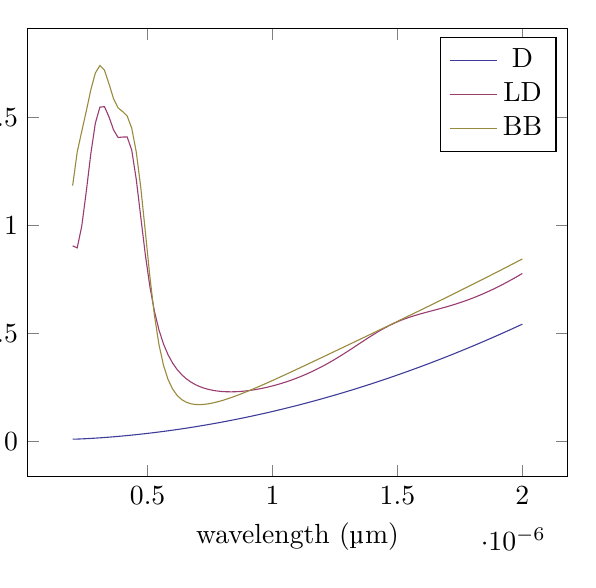
\begin{tikzpicture}[baseline,trim axis left]
\begin{axis}[xlabel=wavelength (\si{\micro\meter}),ylabel=$n'$]
\addplot[color=colora] coordinates {
(2e-07, 0.0088071111912)
(2.18181818182e-07, 0.00933459728886)
(2.36363636364e-07, 0.0101673791713)
(2.54545454545e-07, 0.0111920997537)
(2.72727272727e-07, 0.012363206703)
(2.90909090909e-07, 0.0136587088404)
(3.09090909091e-07, 0.0150666527852)
(3.27272727273e-07, 0.0165799740774)
(3.45454545455e-07, 0.0181942281678)
(3.63636363636e-07, 0.0199064792607)
(3.81818181818e-07, 0.0217147107491)
(4e-07, 0.0236174919937)
(4.18181818182e-07, 0.025613780093)
(4.36363636364e-07, 0.0277027968525)
(4.54545454545e-07, 0.0298839496519)
(4.72727272727e-07, 0.0321567789699)
(4.90909090909e-07, 0.0345209226584)
(5.09090909091e-07, 0.036976091051)
(5.27272727273e-07, 0.0395220492653)
(5.45454545455e-07, 0.0421586043916)
(5.63636363636e-07, 0.044885596066)
(5.81818181818e-07, 0.0477028894342)
(6e-07, 0.0506103698293)
(6.18181818182e-07, 0.0536079386973)
(6.36363636364e-07, 0.0566955104445)
(6.54545454545e-07, 0.0598730099727)
(6.72727272727e-07, 0.0631403707351)
(6.90909090909e-07, 0.0664975331888)
(7.09090909091e-07, 0.0699444435542)
(7.27272727273e-07, 0.0734810528126)
(7.45454545455e-07, 0.0771073158902)
(7.63636363636e-07, 0.080823190991)
(7.81818181818e-07, 0.0846286390465)
(8e-07, 0.0885236232604)
(8.18181818182e-07, 0.0925081087293)
(8.36363636364e-07, 0.0965820621255)
(8.54545454545e-07, 0.10074545143)
(8.72727272727e-07, 0.104998245707)
(8.90909090909e-07, 0.109340414912)
(9.09090909091e-07, 0.113771929733)
(9.27272727273e-07, 0.118292761445)
(9.45454545455e-07, 0.122902881797)
(9.63636363636e-07, 0.127602262905)
(9.81818181818e-07, 0.132390877165)
(1e-06, 0.137268697176)
(1.01818181818e-06, 0.142235695676)
(1.03636363636e-06, 0.147291845478)
(1.05454545455e-06, 0.152437119424)
(1.07272727273e-06, 0.15767149034)
(1.09090909091e-06, 0.162994930996)
(1.10909090909e-06, 0.16840741407)
(1.12727272727e-06, 0.173908912122)
(1.14545454545e-06, 0.179499397565)
(1.16363636364e-06, 0.185178842641)
(1.18181818182e-06, 0.190947219398)
(1.2e-06, 0.196804499677)
(1.21818181818e-06, 0.202750655092)
(1.23636363636e-06, 0.208785657012)
(1.25454545455e-06, 0.214909476556)
(1.27272727273e-06, 0.221122084572)
(1.29090909091e-06, 0.227423451634)
(1.30909090909e-06, 0.233813548027)
(1.32727272727e-06, 0.240292343744)
(1.34545454545e-06, 0.246859808471)
(1.36363636364e-06, 0.253515911588)
(1.38181818182e-06, 0.260260622158)
(1.4e-06, 0.267093908922)
(1.41818181818e-06, 0.274015740296)
(1.43636363636e-06, 0.281026084365)
(1.45454545455e-06, 0.288124908879)
(1.47272727273e-06, 0.295312181249)
(1.49090909091e-06, 0.302587868545)
(1.50909090909e-06, 0.309951937493)
(1.52727272727e-06, 0.317404354469)
(1.54545454545e-06, 0.324945085502)
(1.56363636364e-06, 0.332574096268)
(1.58181818182e-06, 0.340291352089)
(1.6e-06, 0.348096817932)
(1.61818181818e-06, 0.355990458406)
(1.63636363636e-06, 0.363972237763)
(1.65454545455e-06, 0.372042119893)
(1.67272727273e-06, 0.380200068326)
(1.69090909091e-06, 0.388446046232)
(1.70909090909e-06, 0.396780016416)
(1.72727272727e-06, 0.405201941321)
(1.74545454545e-06, 0.413711783024)
(1.76363636364e-06, 0.42230950324)
(1.78181818182e-06, 0.430995063317)
(1.8e-06, 0.439768424238)
(1.81818181818e-06, 0.448629546621)
(1.83636363636e-06, 0.457578390715)
(1.85454545455e-06, 0.466614916407)
(1.87272727273e-06, 0.475739083215)
(1.89090909091e-06, 0.48495085029)
(1.90909090909e-06, 0.494250176418)
(1.92727272727e-06, 0.503637020017)
(1.94545454545e-06, 0.51311133914)
(1.96363636364e-06, 0.522673091472)
(1.98181818182e-06, 0.532322234332)
(2e-06, 0.542058724675)
};
\addlegendentry{D}
\addplot[color=colorb] coordinates {
(2e-07, 0.905310687456)
(2.18181818182e-07, 0.895409655751)
(2.36363636364e-07, 0.995752922549)
(2.54545454545e-07, 1.15644295851)
(2.72727272727e-07, 1.33194256752)
(2.90909090909e-07, 1.4737897699)
(3.09090909091e-07, 1.54799596461)
(3.27272727273e-07, 1.55047949909)
(3.45454545455e-07, 1.50321398694)
(3.63636363636e-07, 1.44286057584)
(3.81818181818e-07, 1.40736579847)
(4e-07, 1.40936964509)
(4.18181818182e-07, 1.41002855744)
(4.36363636364e-07, 1.3495023964)
(4.54545454545e-07, 1.21412184426)
(4.72727272727e-07, 1.0383274037)
(4.90909090909e-07, 0.864147229119)
(5.09090909091e-07, 0.71682689168)
(5.27272727273e-07, 0.602136573101)
(5.45454545455e-07, 0.515500883781)
(5.63636363636e-07, 0.45015084795)
(5.81818181818e-07, 0.400345660786)
(6e-07, 0.361879890824)
(6.18181818182e-07, 0.331800419584)
(6.36363636364e-07, 0.308041985423)
(6.54545454545e-07, 0.289144502399)
(6.72727272727e-07, 0.274058768764)
(6.90909090909e-07, 0.262017411032)
(7.09090909091e-07, 0.252449438252)
(7.27272727273e-07, 0.244923137339)
(7.45454545455e-07, 0.239107349553)
(7.63636363636e-07, 0.2347447778)
(7.81818181818e-07, 0.231633279033)
(8e-07, 0.229612541231)
(8.18181818182e-07, 0.228554451009)
(8.36363636364e-07, 0.228356031643)
(8.54545454545e-07, 0.228934198975)
(8.72727272727e-07, 0.230221821634)
(8.90909090909e-07, 0.232164729641)
(9.09090909091e-07, 0.234719420837)
(9.27272727273e-07, 0.23785128595)
(9.45454545455e-07, 0.241533221929)
(9.63636363636e-07, 0.245744536833)
(9.81818181818e-07, 0.250470072726)
(1e-06, 0.255699488862)
(1.01818181818e-06, 0.26142665797)
(1.03636363636e-06, 0.267649134962)
(1.05454545455e-06, 0.274367660855)
(1.07272727273e-06, 0.281585665684)
(1.09090909091e-06, 0.289308733253)
(1.10909090909e-06, 0.297543988092)
(1.12727272727e-06, 0.306299361683)
(1.14545454545e-06, 0.315582691613)
(1.16363636364e-06, 0.325400605204)
(1.18181818182e-06, 0.335757140249)
(1.2e-06, 0.346652062551)
(1.21818181818e-06, 0.358078856714)
(1.23636363636e-06, 0.370022397571)
(1.25454545455e-06, 0.382456359502)
(1.27272727273e-06, 0.395340493255)
(1.29090909091e-06, 0.408617994967)
(1.30909090909e-06, 0.422213303336)
(1.32727272727e-06, 0.43603077133)
(1.34545454545e-06, 0.449954738075)
(1.36363636364e-06, 0.463851532508)
(1.38181818182e-06, 0.47757382645)
(1.4e-06, 0.490967488094)
(1.41818181818e-06, 0.503880670822)
(1.43636363636e-06, 0.516174368452)
(1.45454545455e-06, 0.527733198176)
(1.47272727273e-06, 0.538474891984)
(1.49090909091e-06, 0.548357016883)
(1.50909090909e-06, 0.55737984549)
(1.52727272727e-06, 0.565584978686)
(1.54545454545e-06, 0.57305009397)
(1.56363636364e-06, 0.579880838652)
(1.58181818182e-06, 0.58620124366)
(1.6e-06, 0.592144050766)
(1.61818181818e-06, 0.597842084445)
(1.63636363636e-06, 0.60342138637)
(1.65454545455e-06, 0.608996399714)
(1.67272727273e-06, 0.614667138606)
(1.69090909091e-06, 0.620518049621)
(1.70909090909e-06, 0.626618166186)
(1.72727272727e-06, 0.633022145979)
(1.74545454545e-06, 0.639771830047)
(1.76363636364e-06, 0.646898038544)
(1.78181818182e-06, 0.654422398635)
(1.8e-06, 0.66235907198)
(1.81818181818e-06, 0.670716306366)
(1.83636363636e-06, 0.679497777761)
(1.85454545455e-06, 0.688703717011)
(1.87272727273e-06, 0.698331832552)
(1.89090909091e-06, 0.708378049706)
(1.90909090909e-06, 0.718837090968)
(1.92727272727e-06, 0.729702922058)
(1.94545454545e-06, 0.740969087015)
(1.96363636364e-06, 0.752628953003)
(1.98181818182e-06, 0.764675882619)
(2e-06, 0.777103348597)
};
\addlegendentry{LD}
\addplot[color=colorc] coordinates {
(2e-07, 1.18438199652)
(2.18181818182e-07, 1.33933500691)
(2.36363636364e-07, 1.43537337185)
(2.54545454545e-07, 1.52954058123)
(2.72727272727e-07, 1.62801861512)
(2.90909090909e-07, 1.70654690527)
(3.09090909091e-07, 1.74067245185)
(3.27272727273e-07, 1.71984873827)
(3.45454545455e-07, 1.65664615059)
(3.63636363636e-07, 1.58720724819)
(3.81818181818e-07, 1.54455097923)
(4e-07, 1.52760574646)
(4.18181818182e-07, 1.50707414608)
(4.36363636364e-07, 1.4511607216)
(4.54545454545e-07, 1.34106990356)
(4.72727272727e-07, 1.17531011499)
(4.90909090909e-07, 0.971214988635)
(5.09090909091e-07, 0.76266020046)
(5.27272727273e-07, 0.583404834209)
(5.45454545455e-07, 0.447624281715)
(5.63636363636e-07, 0.351638495206)
(5.81818181818e-07, 0.285870209994)
(6e-07, 0.241470235982)
(6.18181818182e-07, 0.211857116658)
(6.36363636364e-07, 0.192477711001)
(6.54545454545e-07, 0.180256317381)
(6.72727272727e-07, 0.173123390592)
(6.90909090909e-07, 0.169678171254)
(7.09090909091e-07, 0.168961422026)
(7.27272727273e-07, 0.170305942951)
(7.45454545455e-07, 0.173239094678)
(7.63636363636e-07, 0.177419292251)
(7.81818181818e-07, 0.182594470747)
(8e-07, 0.188574721119)
(8.18181818182e-07, 0.195214079627)
(8.36363636364e-07, 0.202398258373)
(8.54545454545e-07, 0.21003626009)
(8.72727272727e-07, 0.21805455631)
(8.90909090909e-07, 0.226392976162)
(9.09090909091e-07, 0.235001751194)
(9.27272727273e-07, 0.243839352309)
(9.45454545455e-07, 0.252870877539)
(9.63636363636e-07, 0.262066828873)
(9.81818181818e-07, 0.271402168272)
(1e-06, 0.280855577321)
(1.01818181818e-06, 0.290408867821)
(1.03636363636e-06, 0.300046506045)
(1.05454545455e-06, 0.309755223944)
(1.07272727273e-06, 0.319523697845)
(1.09090909091e-06, 0.329342280282)
(1.10909090909e-06, 0.339202774213)
(1.12727272727e-06, 0.349098241476)
(1.14545454545e-06, 0.359022839189)
(1.16363636364e-06, 0.368971679234)
(1.18181818182e-06, 0.378940706937)
(1.2e-06, 0.388926595895)
(1.21818181818e-06, 0.398926656451)
(1.23636363636e-06, 0.408938755793)
(1.25454545455e-06, 0.418961248023)
(1.27272727273e-06, 0.428992912804)
(1.29090909091e-06, 0.43903290143)
(1.30909090909e-06, 0.449080689344)
(1.32727272727e-06, 0.459136034285)
(1.34545454545e-06, 0.469198939344)
(1.36363636364e-06, 0.479269620339)
(1.38181818182e-06, 0.489348476973)
(1.4e-06, 0.499436067333)
(1.41818181818e-06, 0.509533085335)
(1.43636363636e-06, 0.51964034077)
(1.45454545455e-06, 0.529758741654)
(1.47272727273e-06, 0.539889278621)
(1.49090909091e-06, 0.550033011123)
(1.50909090909e-06, 0.560191055237)
(1.52727272727e-06, 0.570364572904)
(1.54545454545e-06, 0.580554762434)
(1.56363636364e-06, 0.590762850137)
(1.58181818182e-06, 0.60099008296)
(1.6e-06, 0.611237722024)
(1.61818181818e-06, 0.621507036944)
(1.63636363636e-06, 0.631799300868)
(1.65454545455e-06, 0.642115786142)
(1.67272727273e-06, 0.652457760534)
(1.69090909091e-06, 0.662826483964)
(1.70909090909e-06, 0.673223205674)
(1.72727272727e-06, 0.683649161792)
(1.74545454545e-06, 0.694105573254)
(1.76363636364e-06, 0.704593644031)
(1.78181818182e-06, 0.715114559642)
(1.8e-06, 0.725669485901)
(1.81818181818e-06, 0.736259567901)
(1.83636363636e-06, 0.746885929169)
(1.85454545455e-06, 0.757549671015)
(1.87272727273e-06, 0.768251872012)
(1.89090909091e-06, 0.778993587626)
(1.90909090909e-06, 0.789775849949)
(1.92727272727e-06, 0.800599667551)
(1.94545454545e-06, 0.811466025407)
(1.96363636364e-06, 0.822375884914)
(1.98181818182e-06, 0.833330183971)
(2e-06, 0.844329837124)
};
\addlegendentry{BB}
\end{axis}
\end{tikzpicture}%
\\
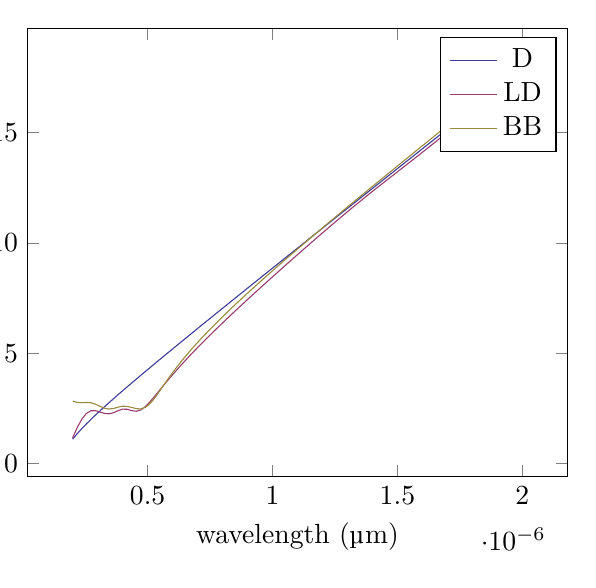
\begin{tikzpicture}[baseline,trim axis left]
\begin{axis}[xlabel=wavelength (\si{\micro\meter}),ylabel=$n''$]
\addplot[color=colora] coordinates {
(2e-07, 1.10681687343)
(2.18181818182e-07, 1.35573033431)
(2.36363636364e-07, 1.58248514026)
(2.54545454545e-07, 1.7954944035)
(2.72727272727e-07, 1.99915542929)
(2.90909090909e-07, 2.19606951316)
(3.09090909091e-07, 2.38790536025)
(3.27272727273e-07, 2.57579688628)
(3.45454545455e-07, 2.7605486611)
(3.63636363636e-07, 2.9427511825)
(3.81818181818e-07, 3.12284977969)
(4e-07, 3.30118791035)
(4.18181818182e-07, 3.47803549383)
(4.36363636364e-07, 3.6536080865)
(4.54545454545e-07, 3.82808023263)
(4.72727272727e-07, 4.00159498846)
(4.90909090909e-07, 4.17427086067)
(5.09090909091e-07, 4.34620695508)
(5.27272727273e-07, 4.51748685977)
(5.45454545455e-07, 4.68818161646)
(5.63636363636e-07, 4.85835202372)
(5.81818181818e-07, 5.02805044341)
(6e-07, 5.19732223244)
(6.18181818182e-07, 5.36620688869)
(6.36363636364e-07, 5.53473897616)
(6.54545454545e-07, 5.70294887815)
(6.72727272727e-07, 5.87086341487)
(6.90909090909e-07, 6.03850635353)
(7.09090909091e-07, 6.2058988323)
(7.27272727273e-07, 6.37305971478)
(7.45454545455e-07, 6.54000588813)
(7.63636363636e-07, 6.706752515)
(7.81818181818e-07, 6.87331324759)
(8e-07, 7.03970041027)
(8.18181818182e-07, 7.20592515618)
(8.36363636364e-07, 7.37199760192)
(8.54545454545e-07, 7.53792694403)
(8.72727272727e-07, 7.70372155989)
(8.90909090909e-07, 7.86938909559)
(9.09090909091e-07, 8.03493654268)
(9.27272727273e-07, 8.2003703053)
(9.45454545455e-07, 8.36569625926)
(9.63636363636e-07, 8.530919804)
(9.81818181818e-07, 8.69604590858)
(1e-06, 8.86107915238)
(1.01818181818e-06, 9.0260237612)
(1.03636363636e-06, 9.19088363948)
(1.05454545455e-06, 9.355662399)
(1.07272727273e-06, 9.52036338451)
(1.09090909091e-06, 9.6849896968)
(1.10909090909e-06, 9.84954421328)
(1.12727272727e-06, 10.0140296066)
(1.14545454545e-06, 10.1784483615)
(1.16363636364e-06, 10.3428027896)
(1.18181818182e-06, 10.5070950437)
(1.2e-06, 10.6713271293)
(1.21818181818e-06, 10.8355009169)
(1.23636363636e-06, 10.9996181513)
(1.25454545455e-06, 11.1636804615)
(1.27272727273e-06, 11.3276893688)
(1.29090909091e-06, 11.4916462952)
(1.30909090909e-06, 11.6555525696)
(1.32727272727e-06, 11.8194094349)
(1.34545454545e-06, 11.983218054)
(1.36363636364e-06, 12.1469795148)
(1.38181818182e-06, 12.3106948358)
(1.4e-06, 12.4743649702)
(1.41818181818e-06, 12.6379908105)
(1.43636363636e-06, 12.8015731923)
(1.45454545455e-06, 12.9651128981)
(1.47272727273e-06, 13.1286106603)
(1.49090909091e-06, 13.2920671646)
(1.50909090909e-06, 13.455483053)
(1.52727272727e-06, 13.618858926)
(1.54545454545e-06, 13.7821953454)
(1.56363636364e-06, 13.9454928367)
(1.58181818182e-06, 14.108751891)
(1.6e-06, 14.2719729669)
(1.61818181818e-06, 14.4351564928)
(1.63636363636e-06, 14.5983028682)
(1.65454545455e-06, 14.7614124656)
(1.67272727273e-06, 14.9244856317)
(1.69090909091e-06, 15.0875226891)
(1.70909090909e-06, 15.2505239374)
(1.72727272727e-06, 15.4134896547)
(1.74545454545e-06, 15.5764200985)
(1.76363636364e-06, 15.7393155067)
(1.78181818182e-06, 15.9021760991)
(1.8e-06, 16.0650020777)
(1.81818181818e-06, 16.2277936283)
(1.83636363636e-06, 16.3905509206)
(1.85454545455e-06, 16.5532741095)
(1.87272727273e-06, 16.7159633359)
(1.89090909091e-06, 16.8786187269)
(1.90909090909e-06, 17.041240397)
(1.92727272727e-06, 17.2038284482)
(1.94545454545e-06, 17.3663829713)
(1.96363636364e-06, 17.5289040456)
(1.98181818182e-06, 17.6913917401)
(2e-06, 17.8538461137)
};
\addlegendentry{D}
\addplot[color=colorb] coordinates {
(2e-07, 1.16819346575)
(2.18181818182e-07, 1.62896170336)
(2.36363636364e-07, 2.00776734752)
(2.54545454545e-07, 2.26785006015)
(2.72727272727e-07, 2.39376305428)
(2.90909090909e-07, 2.40010114338)
(3.09090909091e-07, 2.33864292115)
(3.27272727273e-07, 2.27446967314)
(3.45454545455e-07, 2.25711205272)
(3.63636363636e-07, 2.30570644712)
(3.81818181818e-07, 2.39777817712)
(4e-07, 2.46879979777)
(4.18181818182e-07, 2.46170867615)
(4.36363636364e-07, 2.40170171414)
(4.54545454545e-07, 2.37306527103)
(4.72727272727e-07, 2.43204386456)
(4.90909090909e-07, 2.58161151468)
(5.09090909091e-07, 2.7935406238)
(5.27272727273e-07, 3.0362663467)
(5.45454545455e-07, 3.28892344277)
(5.63636363636e-07, 3.54108691268)
(5.81818181818e-07, 3.78845261451)
(6e-07, 4.02965081767)
(6.18181818182e-07, 4.2645835421)
(6.36363636364e-07, 4.49365455689)
(6.54545454545e-07, 4.7174298676)
(6.72727272727e-07, 4.9364935434)
(6.90909090909e-07, 5.15139052963)
(7.09090909091e-07, 5.36260775946)
(7.27272727273e-07, 5.57057171627)
(7.45454545455e-07, 5.77565261578)
(7.63636363636e-07, 5.97817080559)
(7.81818181818e-07, 6.17840345839)
(8e-07, 6.376590772)
(8.18181818182e-07, 6.57294140779)
(8.36363636364e-07, 6.7676371288)
(8.54545454545e-07, 6.96083669365)
(8.72727272727e-07, 7.15267909431)
(8.90909090909e-07, 7.34328622979)
(9.09090909091e-07, 7.53276509977)
(9.27272727273e-07, 7.72120959048)
(9.45454545455e-07, 7.90870191209)
(9.63636363636e-07, 8.09531373585)
(9.81818181818e-07, 8.2811070686)
(1e-06, 8.46613489398)
(1.01818181818e-06, 8.65044160296)
(1.03636363636e-06, 8.83406323111)
(1.05454545455e-06, 9.01702751672)
(1.07272727273e-06, 9.19935379303)
(1.09090909091e-06, 9.38105272881)
(1.10909090909e-06, 9.56212593655)
(1.12727272727e-06, 9.74256547602)
(1.14545454545e-06, 9.92235329498)
(1.16363636364e-06, 10.1014606691)
(1.18181818182e-06, 10.2798477308)
(1.2e-06, 10.4574632109)
(1.21818181818e-06, 10.6342445615)
(1.23636363636e-06, 10.8101186679)
(1.25454545455e-06, 10.9850034042)
(1.27272727273e-06, 11.158810304)
(1.29090909091e-06, 11.3314486089)
(1.30909090909e-06, 11.5028308843)
(1.32727272727e-06, 11.6728802372)
(1.34545454545e-06, 11.8415389163)
(1.36363636364e-06, 12.0087777304)
(1.38181818182e-06, 12.1746053238)
(1.4e-06, 12.3390759952)
(1.41818181818e-06, 12.5022945587)
(1.43636363636e-06, 12.6644168595)
(1.45454545455e-06, 12.8256450446)
(1.47272727273e-06, 12.9862175208)
(1.49090909091e-06, 13.1463945336)
(1.50909090909e-06, 13.3064411958)
(1.52727272727e-06, 13.4666103109)
(1.54545454545e-06, 13.6271273158)
(1.56363636364e-06, 13.788179121)
(1.58181818182e-06, 13.9499077666)
(1.6e-06, 14.1124088844)
(1.61818181818e-06, 14.2757342238)
(1.63636363636e-06, 14.4398970711)
(1.65454545455e-06, 14.6048792934)
(1.67272727273e-06, 14.7706388794)
(1.69090909091e-06, 14.9371171317)
(1.70909090909e-06, 15.1042449766)
(1.72727272727e-06, 15.2719481309)
(1.74545454545e-06, 15.4401510815)
(1.76363636364e-06, 15.6087799604)
(1.78181818182e-06, 15.7777644763)
(1.8e-06, 15.9470390855)
(1.81818181818e-06, 16.1165435814)
(1.83636363636e-06, 16.2862232622)
(1.85454545455e-06, 16.4560288057)
(1.87272727273e-06, 16.6259159571)
(1.89090909091e-06, 16.7958451038)
(1.90909090909e-06, 16.9657807958)
(1.92727272727e-06, 17.1356912496)
(1.94545454545e-06, 17.3055478605)
(1.96363636364e-06, 17.475324741)
(1.98181818182e-06, 17.644998293)
(2e-06, 17.8145468198)
};
\addlegendentry{LD}
\addplot[color=colorc] coordinates {
(2e-07, 2.83219833386)
(2.18181818182e-07, 2.7731050742)
(2.36363636364e-07, 2.75962713438)
(2.54545454545e-07, 2.77218529699)
(2.72727272727e-07, 2.7579551954)
(2.90909090909e-07, 2.69575082391)
(3.09090909091e-07, 2.60099763553)
(3.27272727273e-07, 2.51173771665)
(3.45454545455e-07, 2.47188668255)
(3.63636363636e-07, 2.49923757993)
(3.81818181818e-07, 2.56091774575)
(4e-07, 2.60184625537)
(4.18181818182e-07, 2.59328196061)
(4.36363636364e-07, 2.54519507631)
(4.54545454545e-07, 2.49222931999)
(4.72727272727e-07, 2.47841492267)
(4.90909090909e-07, 2.54438348471)
(5.09090909091e-07, 2.70893885144)
(5.27272727273e-07, 2.95444973644)
(5.45454545455e-07, 3.24283694059)
(5.63636363636e-07, 3.54302764677)
(5.81818181818e-07, 3.83861774224)
(6e-07, 4.1231601105)
(6.18181818182e-07, 4.39513574524)
(6.36363636364e-07, 4.6551070711)
(6.54545454545e-07, 4.90436614758)
(6.72727272727e-07, 5.14434271255)
(6.90909090909e-07, 5.3763675227)
(7.09090909091e-07, 5.60159531614)
(7.27272727273e-07, 5.82099633162)
(7.45454545455e-07, 6.03537428802)
(7.63636363636e-07, 6.24539208559)
(7.81818181818e-07, 6.45159722909)
(8e-07, 6.65444409779)
(8.18181818182e-07, 6.85431235563)
(8.36363636364e-07, 7.05152173375)
(8.54545454545e-07, 7.24634372541)
(8.72727272727e-07, 7.43901077846)
(8.90909090909e-07, 7.62972351207)
(9.09090909091e-07, 7.81865639452)
(9.27272727273e-07, 8.00596222993)
(9.45454545455e-07, 8.19177572477)
(9.63636363636e-07, 8.37621634229)
(9.81818181818e-07, 8.559390604)
(1e-06, 8.74139395978)
(1.01818181818e-06, 8.9223123193)
(1.03636363636e-06, 9.10222331603)
(1.05454545455e-06, 9.28119735841)
(1.07272727273e-06, 9.45929851076)
(1.09090909091e-06, 9.63658523656)
(1.10909090909e-06, 9.81311103023)
(1.12727272727e-06, 9.98892495744)
(1.14545454545e-06, 10.1640721202)
(1.16363636364e-06, 10.3385940594)
(1.18181818182e-06, 10.5125291056)
(1.2e-06, 10.6859126855)
(1.21818181818e-06, 10.8587775918)
(1.23636363636e-06, 11.0311542213)
(1.25454545455e-06, 11.2030707866)
(1.27272727273e-06, 11.3745535039)
(1.29090909091e-06, 11.5456267613)
(1.30909090909e-06, 11.7163132695)
(1.32727272727e-06, 11.8866341979)
(1.34545454545e-06, 12.0566092963)
(1.36363636364e-06, 12.2262570061)
(1.38181818182e-06, 12.3955945605)
(1.4e-06, 12.5646380755)
(1.41818181818e-06, 12.7334026333)
(1.43636363636e-06, 12.9019023578)
(1.45454545455e-06, 13.0701504841)
(1.47272727273e-06, 13.2381594216)
(1.49090909091e-06, 13.4059408127)
(1.50909090909e-06, 13.5735055857)
(1.52727272727e-06, 13.7408640046)
(1.54545454545e-06, 13.9080257134)
(1.56363636364e-06, 14.074999779)
(1.58181818182e-06, 14.2417947288)
(1.6e-06, 14.4084185867)
(1.61818181818e-06, 14.5748789061)
(1.63636363636e-06, 14.7411828003)
(1.65454545455e-06, 14.9073369706)
(1.67272727273e-06, 15.0733477328)
(1.69090909091e-06, 15.2392210414)
(1.70909090909e-06, 15.4049625122)
(1.72727272727e-06, 15.5705774434)
(1.74545454545e-06, 15.736070835)
(1.76363636364e-06, 15.9014474072)
(1.78181818182e-06, 16.0667116173)
(1.8e-06, 16.2318676754)
(1.81818181818e-06, 16.3969195594)
(1.83636363636e-06, 16.5618710286)
(1.85454545455e-06, 16.7267256364)
(1.87272727273e-06, 16.8914867429)
(1.89090909091e-06, 17.0561575254)
(1.90909090909e-06, 17.2207409895)
(1.92727272727e-06, 17.3852399787)
(1.94545454545e-06, 17.5496571835)
(1.96363636364e-06, 17.7139951503)
(1.98181818182e-06, 17.8782562893)
(2e-06, 18.0424428822)
};
\addlegendentry{BB}
\end{axis}
\end{tikzpicture}%
\\
\end{tabular}
\caption{Material parameters for Au based on the Drude, Lorentz-Drude, and Brendel-Bormann models.}
\end{figure}
\clearpage
\newpage
\subsection{Cu}
\begin{figure}[h!]
\centering
\begin{tabular}{l}
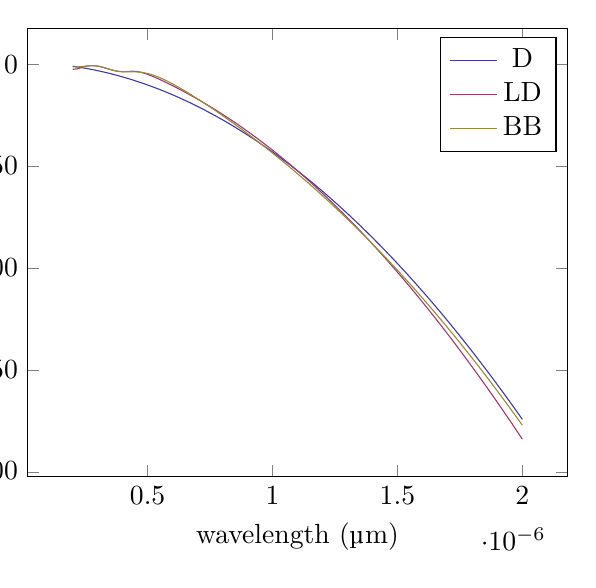
\begin{tikzpicture}[baseline,trim axis left]
\begin{axis}[xlabel=wavelength (\si{\micro\meter}),ylabel=$\epsilon'$]
\addplot[color=colora] coordinates {
(2e-07, -0.754857838768)
(2.18181818182e-07, -1.08841656121)
(2.36363636364e-07, -1.45097702177)
(2.54545454545e-07, -1.84253837845)
(2.72727272727e-07, -2.26309972193)
(2.90909090909e-07, -2.71266007556)
(3.09090909091e-07, -3.19121839534)
(3.27272727273e-07, -3.69877356999)
(3.45454545455e-07, -4.23532442088)
(3.63636363636e-07, -4.8008697021)
(3.81818181818e-07, -5.39540810043)
(4e-07, -6.01893823535)
(4.18181818182e-07, -6.67145865909)
(4.36363636364e-07, -7.35296785656)
(4.54545454545e-07, -8.06346424544)
(4.72727272727e-07, -8.80294617613)
(4.90909090909e-07, -9.57141193181)
(5.09090909091e-07, -10.3688597284)
(5.27272727273e-07, -11.1952877146)
(5.45454545455e-07, -12.0506939718)
(5.63636363636e-07, -12.9350765145)
(5.81818181818e-07, -13.8484332896)
(6e-07, -14.790762177)
(6.18181818182e-07, -15.7620609895)
(6.36363636364e-07, -16.7623274727)
(6.54545454545e-07, -17.791559305)
(6.72727272727e-07, -18.8497540977)
(6.90909090909e-07, -19.9369093949)
(7.09090909091e-07, -21.0530226739)
(7.27272727273e-07, -22.1980913445)
(7.45454545455e-07, -23.3721127497)
(7.63636363636e-07, -24.5750841654)
(7.81818181818e-07, -25.8070028004)
(8e-07, -27.0678657965)
(8.18181818182e-07, -28.3576702285)
(8.36363636364e-07, -29.6764131042)
(8.54545454545e-07, -31.0240913645)
(8.72727272727e-07, -32.4007018831)
(8.90909090909e-07, -33.8062414671)
(9.09090909091e-07, -35.2407068564)
(9.27272727273e-07, -36.7040947242)
(9.45454545455e-07, -38.1964016768)
(9.63636363636e-07, -39.7176242534)
(9.81818181818e-07, -41.2677589266)
(1e-06, -42.8468021021)
(1.01818181818e-06, -44.4547501189)
(1.03636363636e-06, -46.091599249)
(1.05454545455e-06, -47.7573456979)
(1.07272727273e-06, -49.4519856041)
(1.09090909091e-06, -51.1755150396)
(1.10909090909e-06, -52.9279300097)
(1.12727272727e-06, -54.7092264528)
(1.14545454545e-06, -56.5194002409)
(1.16363636364e-06, -58.3584471794)
(1.18181818182e-06, -60.2263630068)
(1.2e-06, -62.1231433954)
(1.21818181818e-06, -64.0487839508)
(1.23636363636e-06, -66.0032802119)
(1.25454545455e-06, -67.9866276514)
(1.27272727273e-06, -69.9988216754)
(1.29090909091e-06, -72.0398576236)
(1.30909090909e-06, -74.1097307691)
(1.32727272727e-06, -76.2084363188)
(1.34545454545e-06, -78.3359694133)
(1.36363636364e-06, -80.4923251268)
(1.38181818182e-06, -82.6774984669)
(1.4e-06, -84.8914843755)
(1.41818181818e-06, -87.1342777277)
(1.43636363636e-06, -89.4058733328)
(1.45454545455e-06, -91.7062659337)
(1.47272727273e-06, -94.0354502071)
(1.49090909091e-06, -96.3934207637)
(1.50909090909e-06, -98.7801721481)
(1.52727272727e-06, -101.195698839)
(1.54545454545e-06, -103.639995248)
(1.56363636364e-06, -106.113055723)
(1.58181818182e-06, -108.614874543)
(1.6e-06, -111.145445924)
(1.61818181818e-06, -113.704764014)
(1.63636363636e-06, -116.292822895)
(1.65454545455e-06, -118.909616586)
(1.67272727273e-06, -121.555139036)
(1.69090909091e-06, -124.229384132)
(1.70909090909e-06, -126.932345693)
(1.72727272727e-06, -129.664017473)
(1.74545454545e-06, -132.42439316)
(1.76363636364e-06, -135.213466378)
(1.78181818182e-06, -138.031230683)
(1.8e-06, -140.877679567)
(1.81818181818e-06, -143.752806456)
(1.83636363636e-06, -146.656604711)
(1.85454545455e-06, -149.589067627)
(1.87272727273e-06, -152.550188433)
(1.89090909091e-06, -155.539960295)
(1.90909090909e-06, -158.558376311)
(1.92727272727e-06, -161.605429515)
(1.94545454545e-06, -164.681112876)
(1.96363636364e-06, -167.785419297)
(1.98181818182e-06, -170.918341617)
(2e-06, -174.079872608)
};
\addlegendentry{D}
\addplot[color=colorb] coordinates {
(2e-07, -2.28414806835)
(2.18181818182e-07, -2.05645654231)
(2.36363636364e-07, -1.40822549503)
(2.54545454545e-07, -0.760882613587)
(2.72727272727e-07, -0.450936556476)
(2.90909090909e-07, -0.53646327192)
(3.09090909091e-07, -0.928641501999)
(3.27272727273e-07, -1.51679792201)
(3.45454545455e-07, -2.19590131908)
(3.63636363636e-07, -2.84678222145)
(3.81818181818e-07, -3.31948955486)
(4e-07, -3.48268652541)
(4.18181818182e-07, -3.36827990528)
(4.36363636364e-07, -3.22697254042)
(4.54545454545e-07, -3.31647904144)
(4.72727272727e-07, -3.71284117343)
(4.90909090909e-07, -4.35950115013)
(5.09090909091e-07, -5.17468353463)
(5.27272727273e-07, -6.09709276475)
(5.45454545455e-07, -7.08934517193)
(5.63636363636e-07, -8.13052900036)
(5.81818181818e-07, -9.20943354528)
(6e-07, -10.3202344776)
(6.18181818182e-07, -11.4600316653)
(6.36363636364e-07, -12.6274970483)
(6.54545454545e-07, -13.8221398346)
(6.72727272727e-07, -15.043907014)
(6.90909090909e-07, -16.292965517)
(7.09090909091e-07, -17.5695833499)
(7.27272727273e-07, -18.8740651256)
(7.45454545455e-07, -20.206717725)
(7.63636363636e-07, -21.5678327337)
(7.81818181818e-07, -22.9576782146)
(8e-07, -24.3764956374)
(8.18181818182e-07, -25.8244995958)
(8.36363636364e-07, -27.3018789674)
(8.54545454545e-07, -28.8087987566)
(8.72727272727e-07, -30.345402191)
(8.90909090909e-07, -31.9118128396)
(9.09090909091e-07, -33.5081366294)
(9.27272727273e-07, -35.1344637035)
(9.45454545455e-07, -36.790870097)
(9.63636363636e-07, -38.4774192322)
(9.81818181818e-07, -40.1941632389)
(1e-06, -41.9411441165)
(1.01818181818e-06, -43.7183947515)
(1.03636363636e-06, -45.5259398084)
(1.05454545455e-06, -47.3637965084)
(1.07272727273e-06, -49.2319753092)
(1.09090909091e-06, -51.1304805002)
(1.10909090909e-06, -53.0593107217)
(1.12727272727e-06, -55.0184594206)
(1.14545454545e-06, -57.0079152484)
(1.16363636364e-06, -59.0276624114)
(1.18181818182e-06, -61.0776809776)
(1.2e-06, -63.1579471461)
(1.21818181818e-06, -65.2684334851)
(1.23636363636e-06, -67.4091091415)
(1.25454545455e-06, -69.579940025)
(1.27272727273e-06, -71.7808889724)
(1.29090909091e-06, -74.0119158913)
(1.30909090909e-06, -76.2729778893)
(1.32727272727e-06, -78.5640293872)
(1.34545454545e-06, -80.8850222209)
(1.36363636364e-06, -83.2359057315)
(1.38181818182e-06, -85.6166268463)
(1.4e-06, -88.0271301513)
(1.41818181818e-06, -90.4673579564)
(1.43636363636e-06, -92.9372503539)
(1.45454545455e-06, -95.4367452723)
(1.47272727273e-06, -97.9657785245)
(1.49090909091e-06, -100.524283852)
(1.50909090909e-06, -103.112192966)
(1.52727272727e-06, -105.729435586)
(1.54545454545e-06, -108.375939474)
(1.56363636364e-06, -111.051630467)
(1.58181818182e-06, -113.756432512)
(1.6e-06, -116.490267691)
(1.61818181818e-06, -119.253056257)
(1.63636363636e-06, -122.044716654)
(1.65454545455e-06, -124.865165553)
(1.67272727273e-06, -127.714317876)
(1.69090909091e-06, -130.592086822)
(1.70909090909e-06, -133.498383899)
(1.72727272727e-06, -136.433118949)
(1.74545454545e-06, -139.39620018)
(1.76363636364e-06, -142.387534191)
(1.78181818182e-06, -145.407026009)
(1.8e-06, -148.454579114)
(1.81818181818e-06, -151.530095478)
(1.83636363636e-06, -154.633475594)
(1.85454545455e-06, -157.764618513)
(1.87272727273e-06, -160.923421883)
(1.89090909091e-06, -164.109781985)
(1.90909090909e-06, -167.323593772)
(1.92727272727e-06, -170.564750918)
(1.94545454545e-06, -173.833145852)
(1.96363636364e-06, -177.128669811)
(1.98181818182e-06, -180.451212886)
(2e-06, -183.80066407)
};
\addlegendentry{LD}
\addplot[color=colorc] coordinates {
(2e-07, -1.09705722702)
(2.18181818182e-07, -1.13001411413)
(2.36363636364e-07, -0.95188611831)
(2.54545454545e-07, -0.681860112848)
(2.72727272727e-07, -0.499448716863)
(2.90909090909e-07, -0.543436800809)
(3.09090909091e-07, -0.878162598981)
(3.27272727273e-07, -1.46685145414)
(3.45454545455e-07, -2.16952479011)
(3.63636363636e-07, -2.80440311259)
(3.81818181818e-07, -3.24004032888)
(4e-07, -3.44869560926)
(4.18181818182e-07, -3.49553846204)
(4.36363636364e-07, -3.49060772005)
(4.54545454545e-07, -3.54121189601)
(4.72727272727e-07, -3.72449232352)
(4.90909090909e-07, -4.08074633847)
(5.09090909091e-07, -4.61944466017)
(5.27272727273e-07, -5.3297217358)
(5.45454545455e-07, -6.1902457928)
(5.63636363636e-07, -7.17642120244)
(5.81818181818e-07, -8.26474437813)
(6e-07, -9.43493076982)
(6.18181818182e-07, -10.6705831794)
(6.36363636364e-07, -11.9590426265)
(6.54545454545e-07, -13.290863732)
(6.72727272727e-07, -14.6591806459)
(6.90909090909e-07, -16.0591022979)
(7.09090909091e-07, -17.4871991309)
(7.27272727273e-07, -18.9410939475)
(7.45454545455e-07, -20.4191520378)
(7.63636363636e-07, -21.9202540714)
(7.81818181818e-07, -23.4436339069)
(8e-07, -24.9887661879)
(8.18181818182e-07, -26.5552891265)
(8.36363636364e-07, -28.1429530091)
(8.54545454545e-07, -29.7515862373)
(8.72727272727e-07, -31.3810732933)
(8.90909090909e-07, -33.0313406043)
(9.09090909091e-07, -34.7023475201)
(9.27272727273e-07, -36.3940805116)
(9.45454545455e-07, -38.1065493356)
(9.63636363636e-07, -39.8397843538)
(9.81818181818e-07, -41.593834497)
(1e-06, -43.3687655637)
(1.01818181818e-06, -45.1646586797)
(1.03636363636e-06, -46.9816088231)
(1.05454545455e-06, -48.819723376)
(1.07272727273e-06, -50.6791206907)
(1.09090909091e-06, -52.559928675)
(1.10909090909e-06, -54.4622834107)
(1.12727272727e-06, -56.3863278194)
(1.14545454545e-06, -58.3322103888)
(1.16363636364e-06, -60.3000839736)
(1.18181818182e-06, -62.2901046768)
(1.2e-06, -64.3024308986)
(1.21818181818e-06, -66.3372220838)
(1.23636363636e-06, -68.3946383421)
(1.25454545455e-06, -70.4748393801)
(1.27272727273e-06, -72.5779839083)
(1.29090909091e-06, -74.704229054)
(1.30909090909e-06, -76.8537298531)
(1.32727272727e-06, -79.0266388141)
(1.34545454545e-06, -81.2231055503)
(1.36363636364e-06, -83.4432764726)
(1.38181818182e-06, -85.687294539)
(1.4e-06, -87.9552990537)
(1.41818181818e-06, -90.2474255117)
(1.43636363636e-06, -92.5638054829)
(1.45454545455e-06, -94.9045665319)
(1.47272727273e-06, -97.2698321685)
(1.49090909091e-06, -99.6597218252)
(1.50909090909e-06, -102.074350858)
(1.52727272727e-06, -104.513830567)
(1.54545454545e-06, -106.978268236)
(1.56363636364e-06, -109.467767182)
(1.58181818182e-06, -111.982426823)
(1.6e-06, -114.522342749)
(1.61818181818e-06, -117.087606807)
(1.63636363636e-06, -119.67830719)
(1.65454545455e-06, -122.294528529)
(1.67272727273e-06, -124.936351991)
(1.69090909091e-06, -127.603855382)
(1.70909090909e-06, -130.297113245)
(1.72727272727e-06, -133.016196966)
(1.74545454545e-06, -135.761174875)
(1.76363636364e-06, -138.532112351)
(1.78181818182e-06, -141.32907192)
(1.8e-06, -144.15211336)
(1.81818181818e-06, -147.001293796)
(1.83636363636e-06, -149.8766678)
(1.85454545455e-06, -152.778287483)
(1.87272727273e-06, -155.706202589)
(1.89090909091e-06, -158.660460585)
(1.90909090909e-06, -161.641106746)
(1.92727272727e-06, -164.648184244)
(1.94545454545e-06, -167.681734225)
(1.96363636364e-06, -170.741795891)
(1.98181818182e-06, -173.828406576)
(2e-06, -176.941601822)
};
\addlegendentry{BB}
\end{axis}
\end{tikzpicture}%
\\
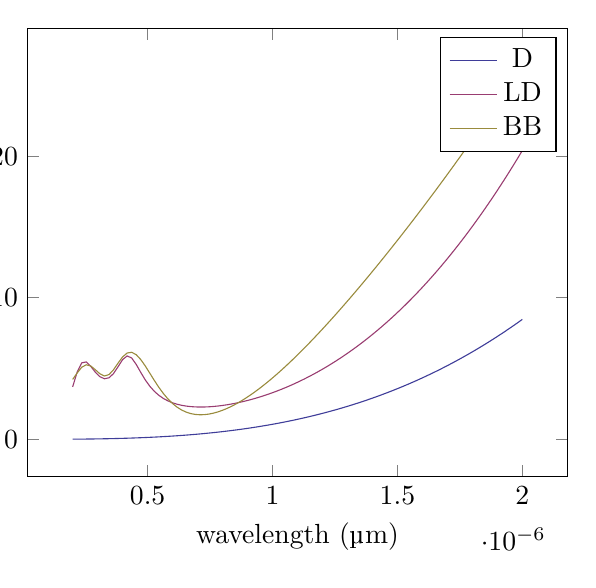
\begin{tikzpicture}[baseline,trim axis left]
\begin{axis}[xlabel=wavelength (\si{\micro\meter}),ylabel=$\epsilon''$]
\addplot[color=colora] coordinates {
(2e-07, 0.00849233017905)
(2.18181818182e-07, 0.0110253052034)
(2.36363636364e-07, 0.014017637923)
(2.54545454545e-07, 0.0175076001198)
(2.72727272727e-07, 0.0215334616496)
(2.90909090909e-07, 0.0261334902941)
(3.09090909091e-07, 0.031345951613)
(3.27272727273e-07, 0.0372091087953)
(3.45454545455e-07, 0.0437612225122)
(3.63636363636e-07, 0.0510405507683)
(3.81818181818e-07, 0.0590853487541)
(4e-07, 0.0679338686977)
(4.18181818182e-07, 0.0776243597174)
(4.36363636364e-07, 0.0881950676729)
(4.54545454545e-07, 0.0996842350183)
(4.72727272727e-07, 0.112130100654)
(4.90909090909e-07, 0.125570899778)
(5.09090909091e-07, 0.14004486374)
(5.27272727273e-07, 0.155590219891)
(5.45454545455e-07, 0.172245191438)
(5.63636363636e-07, 0.190047997296)
(5.81818181818e-07, 0.209036851938)
(6e-07, 0.229249965251)
(6.18181818182e-07, 0.250725542384)
(6.36363636364e-07, 0.273501783605)
(6.54545454545e-07, 0.29761688415)
(6.72727272727e-07, 0.323109034078)
(6.90909090909e-07, 0.350016418121)
(7.09090909091e-07, 0.37837721554)
(7.27272727273e-07, 0.408229599975)
(7.45454545455e-07, 0.439611739297)
(7.63636363636e-07, 0.472561795463)
(7.81818181818e-07, 0.50711792437)
(8e-07, 0.543318275703)
(8.18181818182e-07, 0.581200992791)
(8.36363636364e-07, 0.620804212461)
(8.54545454545e-07, 0.662166064889)
(8.72727272727e-07, 0.705324673455)
(8.90909090909e-07, 0.750318154591)
(9.09090909091e-07, 0.797184617642)
(9.27272727273e-07, 0.845962164713)
(9.45454545455e-07, 0.896688890526)
(9.63636363636e-07, 0.949402882271)
(9.81818181818e-07, 1.00414221946)
(1e-06, 1.06094497378)
(1.01818181818e-06, 1.11984920894)
(1.03636363636e-06, 1.18089298056)
(1.05454545455e-06, 1.24411433596)
(1.07272727273e-06, 1.30955131407)
(1.09090909091e-06, 1.37724194526)
(1.10909090909e-06, 1.4472242512)
(1.12727272727e-06, 1.51953624471)
(1.14545454545e-06, 1.59421592961)
(1.16363636364e-06, 1.6713013006)
(1.18181818182e-06, 1.75083034306)
(1.2e-06, 1.83284103297)
(1.21818181818e-06, 1.91737133672)
(1.23636363636e-06, 2.00445921097)
(1.25454545455e-06, 2.09414260252)
(1.27272727273e-06, 2.18645944817)
(1.29090909091e-06, 2.28144767452)
(1.30909090909e-06, 2.37914519791)
(1.32727272727e-06, 2.4795899242)
(1.34545454545e-06, 2.58281974866)
(1.36363636364e-06, 2.68887255584)
(1.38181818182e-06, 2.79778621938)
(1.4e-06, 2.90959860189)
(1.41818181818e-06, 3.02434755484)
(1.43636363636e-06, 3.14207091833)
(1.45454545455e-06, 3.26280652104)
(1.47272727273e-06, 3.38659218001)
(1.49090909091e-06, 3.51346570054)
(1.50909090909e-06, 3.64346487604)
(1.52727272727e-06, 3.77662748787)
(1.54545454545e-06, 3.9129913052)
(1.56363636364e-06, 4.05259408487)
(1.58181818182e-06, 4.19547357127)
(1.6e-06, 4.34166749614)
(1.61818181818e-06, 4.49121357847)
(1.63636363636e-06, 4.64414952436)
(1.65454545455e-06, 4.80051302684)
(1.67272727273e-06, 4.96034176577)
(1.69090909091e-06, 5.12367340765)
(1.70909090909e-06, 5.29054560552)
(1.72727272727e-06, 5.4609959988)
(1.74545454545e-06, 5.63506221313)
(1.76363636364e-06, 5.81278186026)
(1.78181818182e-06, 5.99419253787)
(1.8e-06, 6.17933182948)
(1.81818181818e-06, 6.36823730424)
(1.83636363636e-06, 6.56094651684)
(1.85454545455e-06, 6.75749700735)
(1.87272727273e-06, 6.95792630107)
(1.89090909091e-06, 7.1622719084)
(1.90909090909e-06, 7.37057132471)
(1.92727272727e-06, 7.58286203015)
(1.94545454545e-06, 7.79918148957)
(1.96363636364e-06, 8.01956715233)
(1.98181818182e-06, 8.24405645219)
(2e-06, 8.47268680715)
};
\addlegendentry{D}
\addplot[color=colorb] coordinates {
(2e-07, 3.70327050075)
(2.18181818182e-07, 4.7597344356)
(2.36363636364e-07, 5.40362084258)
(2.54545454545e-07, 5.46514637693)
(2.72727272727e-07, 5.14875024245)
(2.90909090909e-07, 4.74133151756)
(3.09090909091e-07, 4.42250449365)
(3.27272727273e-07, 4.27678277154)
(3.45454545455e-07, 4.34553351634)
(3.63636363636e-07, 4.64403682698)
(3.81818181818e-07, 5.12862886487)
(4e-07, 5.63303804953)
(4.18181818182e-07, 5.89066354164)
(4.36363636364e-07, 5.74401370018)
(4.54545454545e-07, 5.2879566134)
(4.72727272727e-07, 4.72452947511)
(4.90909090909e-07, 4.19253361479)
(5.09090909091e-07, 3.74431391695)
(5.27272727273e-07, 3.38476547897)
(5.45454545455e-07, 3.1020594032)
(5.63636363636e-07, 2.88152351987)
(5.81818181818e-07, 2.71025067475)
(6e-07, 2.57802414347)
(6.18181818182e-07, 2.47706441802)
(6.36363636364e-07, 2.40151922688)
(6.54545454545e-07, 2.34698643639)
(6.72727272727e-07, 2.31013634477)
(6.90909090909e-07, 2.28843023516)
(7.09090909091e-07, 2.27991541524)
(7.27272727273e-07, 2.28307688176)
(7.45454545455e-07, 2.29672974305)
(7.63636363636e-07, 2.31994070269)
(7.81818181818e-07, 2.35197026043)
(8e-07, 2.39222975209)
(8.18181818182e-07, 2.44024909627)
(8.36363636364e-07, 2.49565233429)
(8.54545454545e-07, 2.5581388958)
(8.72727272727e-07, 2.62746911169)
(8.90909090909e-07, 2.70345290775)
(9.09090909091e-07, 2.78594090275)
(9.27272727273e-07, 2.87481734053)
(9.45454545455e-07, 2.96999443327)
(9.63636363636e-07, 3.07140779959)
(9.81818181818e-07, 3.17901275887)
(1e-06, 3.29278130028)
(1.01818181818e-06, 3.41269958718)
(1.03636363636e-06, 3.53876588932)
(1.05454545455e-06, 3.67098885924)
(1.07272727273e-06, 3.80938608689)
(1.09090909091e-06, 3.95398288093)
(1.10909090909e-06, 4.10481123538)
(1.12727272727e-06, 4.26190894878)
(1.14545454545e-06, 4.42531886943)
(1.16363636364e-06, 4.59508824522)
(1.18181818182e-06, 4.77126816085)
(1.2e-06, 4.95391304811)
(1.21818181818e-06, 5.14308025761)
(1.23636363636e-06, 5.33882968239)
(1.25454545455e-06, 5.54122342539)
(1.27272727273e-06, 5.75032550427)
(1.29090909091e-06, 5.96620158786)
(1.30909090909e-06, 6.18891875986)
(1.32727272727e-06, 6.41854530563)
(1.34545454545e-06, 6.655150519)
(1.36363636364e-06, 6.89880452615)
(1.38181818182e-06, 7.14957812426)
(1.4e-06, 7.40754263289)
(1.41818181818e-06, 7.67276975639)
(1.43636363636e-06, 7.94533145581)
(1.45454545455e-06, 8.22529982908)
(1.47272727273e-06, 8.51274699832)
(1.49090909091e-06, 8.80774500337)
(1.50909090909e-06, 9.11036570074)
(1.52727272727e-06, 9.42068066724)
(1.54545454545e-06, 9.73876110766)
(1.56363636364e-06, 10.064677766)
(1.58181818182e-06, 10.39850084)
(1.6e-06, 10.7402998978)
(1.61818181818e-06, 11.0901437977)
(1.63636363636e-06, 11.4481006094)
(1.65454545455e-06, 11.8142375376)
(1.67272727273e-06, 12.1886208463)
(1.69090909091e-06, 12.5713157855)
(1.70909090909e-06, 12.9623865185)
(1.72727272727e-06, 13.3618960505)
(1.74545454545e-06, 13.7699061583)
(1.76363636364e-06, 14.1864773209)
(1.78181818182e-06, 14.6116686507)
(1.8e-06, 15.0455378256)
(1.81818181818e-06, 15.4881410225)
(1.83636363636e-06, 15.9395328503)
(1.85454545455e-06, 16.3997662846)
(1.87272727273e-06, 16.8688926028)
(1.89090909091e-06, 17.3469613203)
(1.90909090909e-06, 17.8340201266)
(1.92727272727e-06, 18.3301148229)
(1.94545454545e-06, 18.8352892607)
(1.96363636364e-06, 19.3495852805)
(1.98181818182e-06, 19.8730426523)
(2e-06, 20.4056990164)
};
\addlegendentry{LD}
\addplot[color=colorc] coordinates {
(2e-07, 4.2308711043)
(2.18181818182e-07, 4.68598963786)
(2.36363636364e-07, 5.09210411323)
(2.54545454545e-07, 5.26498626742)
(2.72727272727e-07, 5.17841945519)
(2.90909090909e-07, 4.91669436309)
(3.09090909091e-07, 4.62692044157)
(3.27272727273e-07, 4.47479409957)
(3.45454545455e-07, 4.57227769516)
(3.63636363636e-07, 4.91431299531)
(3.81818181818e-07, 5.38419247296)
(4e-07, 5.82160003965)
(4.18181818182e-07, 6.09660660551)
(4.36363636364e-07, 6.14723179552)
(4.54545454545e-07, 5.97717286017)
(4.72727272727e-07, 5.63232238799)
(4.90909090909e-07, 5.17482995315)
(5.09090909091e-07, 4.66447486693)
(5.27272727273e-07, 4.1491370872)
(5.45454545455e-07, 3.66220544385)
(5.63636363636e-07, 3.22393808287)
(5.81818181818e-07, 2.84441719665)
(6e-07, 2.52667992756)
(6.18181818182e-07, 2.26936426981)
(6.36363636364e-07, 2.06867781012)
(6.54545454545e-07, 1.91973249311)
(6.72727272727e-07, 1.81737679459)
(6.90909090909e-07, 1.75666781534)
(7.09090909091e-07, 1.73310447427)
(7.27272727273e-07, 1.74271281905)
(7.45454545455e-07, 1.78204670903)
(7.63636363636e-07, 1.84814503154)
(7.81818181818e-07, 1.93847074675)
(8e-07, 2.0508463218)
(8.18181818182e-07, 2.18339319389)
(8.36363636364e-07, 2.33447871162)
(8.54545454545e-07, 2.50267155622)
(8.72727272727e-07, 2.68670534581)
(8.90909090909e-07, 2.8854495089)
(9.09090909091e-07, 3.09788629655)
(9.27272727273e-07, 3.32309280199)
(9.45454545455e-07, 3.56022696301)
(9.63636363636e-07, 3.80851667074)
(9.81818181818e-07, 4.06725126393)
(1e-06, 4.33577483195)
(1.01818181818e-06, 4.61348087493)
(1.03636363636e-06, 4.89980797385)
(1.05454545455e-06, 5.19423620772)
(1.07272727273e-06, 5.49628412156)
(1.09090909091e-06, 5.80550610065)
(1.10909090909e-06, 6.12149004599)
(1.12727272727e-06, 6.44385527551)
(1.14545454545e-06, 6.77225059787)
(1.16363636364e-06, 7.10635252157)
(1.18181818182e-06, 7.44586357404)
(1.2e-06, 7.79051071597)
(1.21818181818e-06, 8.1400438248)
(1.23636363636e-06, 8.49423427651)
(1.25454545455e-06, 8.85287357234)
(1.27272727273e-06, 9.21577204354)
(1.29090909091e-06, 9.58275761763)
(1.30909090909e-06, 9.95367464678)
(1.32727272727e-06, 10.3283827971)
(1.34545454545e-06, 10.7067559974)
(1.36363636364e-06, 11.0886814461)
(1.38181818182e-06, 11.4740586752)
(1.4e-06, 11.862798668)
(1.41818181818e-06, 12.2548230319)
(1.43636363636e-06, 12.6500632205)
(1.45454545455e-06, 13.0484598064)
(1.47272727273e-06, 13.4499618003)
(1.49090909091e-06, 13.8545260154)
(1.50909090909e-06, 14.2621164741)
(1.52727272727e-06, 14.6727038555)
(1.54545454545e-06, 15.0862649812)
(1.56363636364e-06, 15.502782337)
(1.58181818182e-06, 15.9222436285)
(1.6e-06, 16.3446413689)
(1.61818181818e-06, 16.7699724967)
(1.63636363636e-06, 17.1982380209)
(1.65454545455e-06, 17.6294426931)
(1.67272727273e-06, 18.0635947036)
(1.69090909091e-06, 18.5007054)
(1.70909090909e-06, 18.9407890275)
(1.72727272727e-06, 19.383862489)
(1.74545454545e-06, 19.8299451226)
(1.76363636364e-06, 20.2790584972)
(1.78181818182e-06, 20.7312262232)
(1.8e-06, 21.1864737779)
(1.81818181818e-06, 21.6448283448)
(1.83636363636e-06, 22.1063186648)
(1.85454545455e-06, 22.5709748995)
(1.87272727273e-06, 23.0388285054)
(1.89090909091e-06, 23.5099121172)
(1.90909090909e-06, 23.9842594412)
(1.92727272727e-06, 24.4619051566)
(1.94545454545e-06, 24.9428848247)
(1.96363636364e-06, 25.4272348055)
(1.98181818182e-06, 25.914992181)
(2e-06, 26.4061946842)
};
\addlegendentry{BB}
\end{axis}
\end{tikzpicture}%
\\
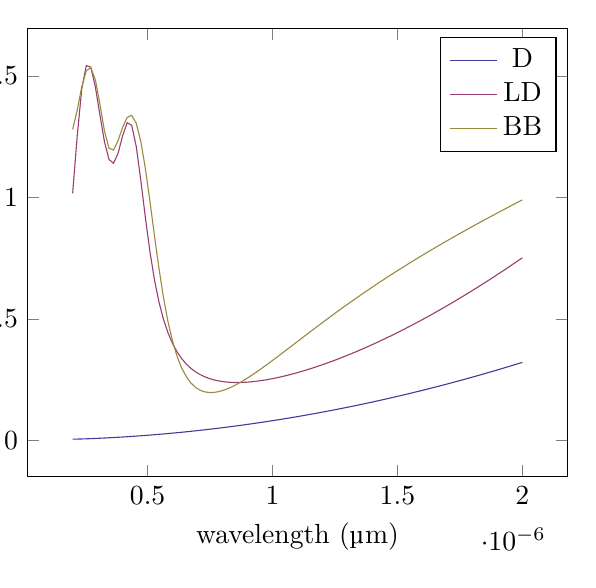
\begin{tikzpicture}[baseline,trim axis left]
\begin{axis}[xlabel=wavelength (\si{\micro\meter}),ylabel=$n'$]
\addplot[color=colora] coordinates {
(2e-07, 0.00488716970616)
(2.18181818182e-07, 0.00528393521233)
(2.36363636364e-07, 0.00581847949753)
(2.54545454545e-07, 0.00644886744896)
(2.72727272727e-07, 0.00715693536678)
(2.90909090909e-07, 0.00793349759931)
(3.09090909091e-07, 0.00877340064552)
(3.27272727273e-07, 0.00967352829057)
(3.45454545455e-07, 0.0106318860596)
(3.63636363636e-07, 0.0116471390711)
(3.81818181818e-07, 0.0127183609958)
(4e-07, 0.0138448894798)
(4.18181818182e-07, 0.0150262388086)
(4.36363636364e-07, 0.0162620450079)
(4.54545454545e-07, 0.0175520301514)
(4.72727272727e-07, 0.0188959784742)
(4.90909090909e-07, 0.0202937199818)
(5.09090909091e-07, 0.0217451189511)
(5.27272727273e-07, 0.0232500657055)
(5.45454545455e-07, 0.0248084706289)
(5.63636363636e-07, 0.0264202597403)
(5.81818181818e-07, 0.0280853713775)
(6e-07, 0.0298037536777)
(6.18181818182e-07, 0.0315753626437)
(6.36363636364e-07, 0.0334001606422)
(6.54545454545e-07, 0.0352781152263)
(6.72727272727e-07, 0.037209198205)
(6.90909090909e-07, 0.0391933849007)
(7.09090909091e-07, 0.0412306535516)
(7.27272727273e-07, 0.0433209848295)
(7.45454545455e-07, 0.0454643614457)
(7.63636363636e-07, 0.047660767828)
(7.81818181818e-07, 0.0499101898543)
(8e-07, 0.0522126146318)
(8.18181818182e-07, 0.0545680303127)
(8.36363636364e-07, 0.0569764259399)
(8.54545454545e-07, 0.0594377913166)
(8.72727272727e-07, 0.061952116897)
(8.90909090909e-07, 0.0645193936926)
(9.09090909091e-07, 0.0671396131926)
(9.27272727273e-07, 0.0698127672964)
(9.45454545455e-07, 0.0725388482542)
(9.63636363636e-07, 0.0753178486177)
(9.81818181818e-07, 0.0781497611956)
(1e-06, 0.0810345790168)
(1.01818181818e-06, 0.0839722952965)
(1.03636363636e-06, 0.0869629034088)
(1.05454545455e-06, 0.0900063968603)
(1.07272727273e-06, 0.0931027692695)
(1.09090909091e-06, 0.0962520143463)
(1.10909090909e-06, 0.0994541258759)
(1.12727272727e-06, 0.102709097703)
(1.14545454545e-06, 0.10601692372)
(1.16363636364e-06, 0.109377597852)
(1.18181818182e-06, 0.112791114051)
(1.2e-06, 0.116257466282)
(1.21818181818e-06, 0.119776648517)
(1.23636363636e-06, 0.123348654729)
(1.25454545455e-06, 0.126973478881)
(1.27272727273e-06, 0.130651114924)
(1.29090909091e-06, 0.134381556789)
(1.30909090909e-06, 0.138164798385)
(1.32727272727e-06, 0.142000833593)
(1.34545454545e-06, 0.14588965626)
(1.36363636364e-06, 0.149831260199)
(1.38181818182e-06, 0.153825639183)
(1.4e-06, 0.157872786946)
(1.41818181818e-06, 0.161972697175)
(1.43636363636e-06, 0.166125363511)
(1.45454545455e-06, 0.170330779547)
(1.47272727273e-06, 0.174588938824)
(1.49090909091e-06, 0.17889983483)
(1.50909090909e-06, 0.183263461001)
(1.52727272727e-06, 0.187679810713)
(1.54545454545e-06, 0.192148877289)
(1.56363636364e-06, 0.19667065399)
(1.58181818182e-06, 0.20124513402)
(1.6e-06, 0.205872310519)
(1.61818181818e-06, 0.210552176569)
(1.63636363636e-06, 0.215284725187)
(1.65454545455e-06, 0.220069949327)
(1.67272727273e-06, 0.224907841877)
(1.69090909091e-06, 0.229798395664)
(1.70909090909e-06, 0.234741603446)
(1.72727272727e-06, 0.239737457915)
(1.74545454545e-06, 0.244785951698)
(1.76363636364e-06, 0.249887077354)
(1.78181818182e-06, 0.255040827374)
(1.8e-06, 0.26024719418)
(1.81818181818e-06, 0.265506170127)
(1.83636363636e-06, 0.270817747501)
(1.85454545455e-06, 0.276181918517)
(1.87272727273e-06, 0.281598675323)
(1.89090909091e-06, 0.287068009995)
(1.90909090909e-06, 0.292589914539)
(1.92727272727e-06, 0.298164380892)
(1.94545454545e-06, 0.30379140092)
(1.96363636364e-06, 0.309470966417)
(1.98181818182e-06, 0.315203069107)
(2e-06, 0.320987700643)
};
\addlegendentry{D}
\addplot[color=colorb] coordinates {
(2e-07, 1.01658532343)
(2.18181818182e-07, 1.25070580004)
(2.36363636364e-07, 1.44497032575)
(2.54545454545e-07, 1.54223479497)
(2.72727272727e-07, 1.535825978)
(2.90909090909e-07, 1.45518402586)
(3.09090909091e-07, 1.33983391104)
(3.27272727273e-07, 1.22902258718)
(3.45454545455e-07, 1.15605858671)
(3.63636363636e-07, 1.14025211737)
(3.81818181818e-07, 1.18103157968)
(4e-07, 1.25300011856)
(4.18181818182e-07, 1.30716934617)
(4.36363636364e-07, 1.29642388558)
(4.54545454545e-07, 1.20942903905)
(4.72727272727e-07, 1.07145142611)
(4.90909090909e-07, 0.918926830149)
(5.09090909091e-07, 0.778648797914)
(5.27272727273e-07, 0.662009445554)
(5.45454545455e-07, 0.56963771472)
(5.63636363636e-07, 0.497753744763)
(5.81818181818e-07, 0.441882834485)
(6e-07, 0.398200000433)
(6.18181818182e-07, 0.363765436984)
(6.36363636364e-07, 0.336403138578)
(6.54545454545e-07, 0.314517211975)
(6.72727272727e-07, 0.296932925871)
(6.90909090909e-07, 0.282777270911)
(7.09090909091e-07, 0.271393595719)
(7.27272727273e-07, 0.262281587222)
(7.45454545455e-07, 0.255055125199)
(7.63636363636e-07, 0.249412510744)
(7.81818181818e-07, 0.24511523447)
(8e-07, 0.241972664973)
(8.18181818182e-07, 0.239830876006)
(8.36363636364e-07, 0.238564396777)
(8.54545454545e-07, 0.238070049836)
(8.72727272727e-07, 0.238262296824)
(8.90909090909e-07, 0.239069685652)
(9.09090909091e-07, 0.240432111047)
(9.27272727273e-07, 0.242298682086)
(9.45454545455e-07, 0.244626047288)
(9.63636363636e-07, 0.247377067915)
(9.81818181818e-07, 0.250519758702)
(1e-06, 0.254026435733)
(1.01818181818e-06, 0.257873026094)
(1.03636363636e-06, 0.262038504842)
(1.05454545455e-06, 0.266504432897)
(1.07272727273e-06, 0.27125457552)
(1.09090909091e-06, 0.27627458551)
(1.10909090909e-06, 0.28155173876)
(1.12727272727e-06, 0.287074712369)
(1.14545454545e-06, 0.292833397578)
(1.16363636364e-06, 0.298818741329)
(1.18181818182e-06, 0.305022611475)
(1.2e-06, 0.311437681639)
(1.21818181818e-06, 0.318057332456)
(1.23636363636e-06, 0.324875566541)
(1.25454545455e-06, 0.331886935008)
(1.27272727273e-06, 0.339086473746)
(1.29090909091e-06, 0.346469647961)
(1.30909090909e-06, 0.354032303767)
(1.32727272727e-06, 0.361770625781)
(1.34545454545e-06, 0.369681099869)
(1.36363636364e-06, 0.377760480321)
(1.38181818182e-06, 0.386005760844)
(1.4e-06, 0.394414148855)
(1.41818181818e-06, 0.402983042637)
(1.43636363636e-06, 0.411710010987)
(1.45454545455e-06, 0.42059277503)
(1.47272727273e-06, 0.429629191942)
(1.49090909091e-06, 0.43881724032)
(1.50909090909e-06, 0.448155007032)
(1.52727272727e-06, 0.457640675342)
(1.54545454545e-06, 0.467272514173)
(1.56363636364e-06, 0.477048868383)
(1.58181818182e-06, 0.486968149924)
(1.6e-06, 0.497028829795)
(1.61818181818e-06, 0.507229430707)
(1.63636363636e-06, 0.517568520372)
(1.65454545455e-06, 0.528044705355)
(1.67272727273e-06, 0.538656625441)
(1.69090909091e-06, 0.549402948442)
(1.70909090909e-06, 0.560282365426)
(1.72727272727e-06, 0.571293586312)
(1.74545454545e-06, 0.582435335796)
(1.76363636364e-06, 0.593706349582)
(1.78181818182e-06, 0.605105370898)
(1.8e-06, 0.61663114725)
(1.81818181818e-06, 0.628282427417)
(1.83636363636e-06, 0.640057958657)
(1.85454545455e-06, 0.651956484101)
(1.87272727273e-06, 0.663976740336)
(1.89090909091e-06, 0.67611745515)
(1.90909090909e-06, 0.688377345431)
(1.92727272727e-06, 0.700755115215)
(1.94545454545e-06, 0.713249453866)
(1.96363636364e-06, 0.725859034384)
(1.98181818182e-06, 0.738582511834)
(2e-06, 0.75141852189)
};
\addlegendentry{LD}
\addplot[color=colorc] coordinates {
(2e-07, 1.27940078384)
(2.18181818182e-07, 1.35836303548)
(2.36363636364e-07, 1.45403298811)
(2.54545454545e-07, 1.52103515217)
(2.72727272727e-07, 1.53346020899)
(2.90909090909e-07, 1.48377881243)
(3.09090909091e-07, 1.38408014033)
(3.27272727273e-07, 1.27322987898)
(3.45454545455e-07, 1.20236446642)
(3.63636363636e-07, 1.19452709817)
(3.81818181818e-07, 1.23366505418)
(4e-07, 1.28796951698)
(4.18181818182e-07, 1.32892410931)
(4.36363636364e-07, 1.33763533347)
(4.54545454545e-07, 1.30503211365)
(4.72727272727e-07, 1.23042820648)
(4.90909090909e-07, 1.12015639016)
(5.09090909091e-07, 0.986244141499)
(5.27272727273e-07, 0.843987668318)
(5.45454545455e-07, 0.70787472411)
(5.63636363636e-07, 0.587751437271)
(5.81818181818e-07, 0.487737996332)
(6e-07, 0.407716513052)
(6.18181818182e-07, 0.345434210956)
(6.36363636364e-07, 0.297994469898)
(6.54545454545e-07, 0.262609417144)
(6.72727272727e-07, 0.236881159906)
(6.90909090909e-07, 0.218852914396)
(7.09090909091e-07, 0.206968073534)
(7.27272727273e-07, 0.200002396603)
(7.45454545455e-07, 0.196996236633)
(7.63636363636e-07, 0.197196129204)
(7.81818181818e-07, 0.20000763608)
(8e-07, 0.204958522352)
(8.18181818182e-07, 0.211670518988)
(8.36363636364e-07, 0.219837872063)
(8.54545454545e-07, 0.229211119038)
(8.72727272727e-07, 0.239584828762)
(8.90909090909e-07, 0.250788320921)
(9.09090909091e-07, 0.26267861441)
(9.27272727273e-07, 0.275135039831)
(9.45454545455e-07, 0.288055094526)
(9.63636363636e-07, 0.301351226964)
(9.81818181818e-07, 0.314948318466)
(1e-06, 0.328781690551)
(1.01818181818e-06, 0.342795510764)
(1.03636363636e-06, 0.356941502756)
(1.05454545455e-06, 0.371177890535)
(1.07272727273e-06, 0.385468524681)
(1.09090909091e-06, 0.399782151353)
(1.10909090909e-06, 0.414091794628)
(1.12727272727e-06, 0.428374229804)
(1.14545454545e-06, 0.442609530581)
(1.16363636364e-06, 0.456780676955)
(1.18181818182e-06, 0.470873213572)
(1.2e-06, 0.484874950332)
(1.21818181818e-06, 0.498775699688)
(1.23636363636e-06, 0.512567043334)
(1.25454545455e-06, 0.526242126906)
(1.27272727273e-06, 0.539795477118)
(1.29090909091e-06, 0.553222839275)
(1.30909090909e-06, 0.566521032579)
(1.32727272727e-06, 0.579687821164)
(1.34545454545e-06, 0.592721799053)
(1.36363636364e-06, 0.605622287516)
(1.38181818182e-06, 0.618389243456)
(1.4e-06, 0.631023177655)
(1.41818181818e-06, 0.643525081828)
(1.43636363636e-06, 0.65589636356)
(1.45454545455e-06, 0.66813878831)
(1.47272727273e-06, 0.680254427743)
(1.49090909091e-06, 0.692245613732)
(1.50909090909e-06, 0.70411489746)
(1.52727272727e-06, 0.71586501308)
(1.54545454545e-06, 0.727498845464)
(1.56363636364e-06, 0.739019401636)
(1.58181818182e-06, 0.75042978548)
(1.6e-06, 0.76173317541)
(1.61818181818e-06, 0.772932804671)
(1.63636363636e-06, 0.784031944017)
(1.65454545455e-06, 0.795033886501)
(1.67272727273e-06, 0.805941934154)
(1.69090909091e-06, 0.816759386372)
(1.70909090909e-06, 0.827489529804)
(1.72727272727e-06, 0.838135629597)
(1.74545454545e-06, 0.848700921844)
(1.76363636364e-06, 0.859188607111)
(1.78181818182e-06, 0.869601844916)
(1.8e-06, 0.879943749063)
(1.81818181818e-06, 0.890217383728)
(1.83636363636e-06, 0.900425760224)
(1.85454545455e-06, 0.910571834355)
(1.87272727273e-06, 0.920658504297)
(1.89090909091e-06, 0.930688608949)
(1.90909090909e-06, 0.940664926691)
(1.92727272727e-06, 0.950590174503)
(1.94545454545e-06, 0.960467007402)
(1.96363636364e-06, 0.970298018159)
(1.98181818182e-06, 0.980085737255)
(2e-06, 0.989832633052)
};
\addlegendentry{BB}
\end{axis}
\end{tikzpicture}%
\\
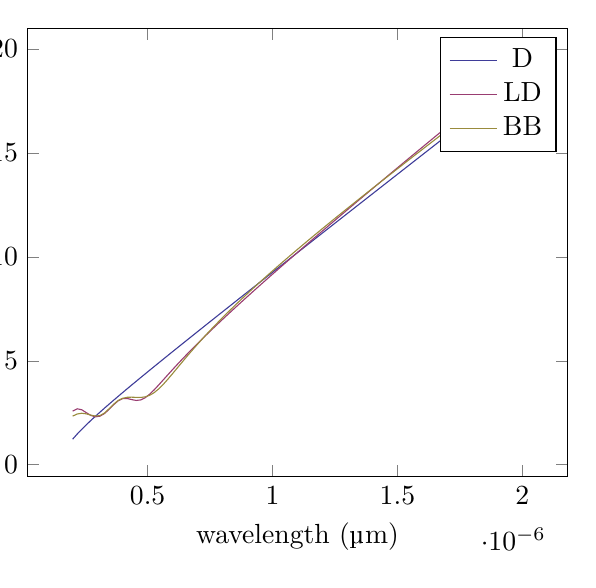
\begin{tikzpicture}[baseline,trim axis left]
\begin{axis}[xlabel=wavelength (\si{\micro\meter}),ylabel=$n''$]
\addplot[color=colora] coordinates {
(2e-07, 1.22872431668)
(2.18181818182e-07, 1.47542839961)
(2.36363636364e-07, 1.70353214027)
(2.54545454545e-07, 1.91967703864)
(2.72727272727e-07, 2.12751072555)
(2.90909090909e-07, 2.3292586872)
(3.09090909091e-07, 2.52637897707)
(3.27272727273e-07, 2.71987762487)
(3.45454545455e-07, 2.9104767506)
(3.63636363636e-07, 3.09871113786)
(3.81818181818e-07, 3.28498701889)
(4e-07, 3.46961955157)
(4.18181818182e-07, 3.65285763395)
(4.36363636364e-07, 3.834900862)
(4.54545454545e-07, 4.01591143309)
(4.72727272727e-07, 4.19602269635)
(4.90909090909e-07, 4.37534541879)
(5.09090909091e-07, 4.55397245898)
(5.27272727273e-07, 4.73198230769)
(5.45454545455e-07, 4.90944180779)
(5.63636363636e-07, 5.08640827001)
(5.81818181818e-07, 5.26293113724)
(6e-07, 5.43905330747)
(6.18181818182e-07, 5.61481219509)
(6.36363636364e-07, 5.79024058972)
(6.54545454545e-07, 5.96536735673)
(6.72727272727e-07, 6.14021801276)
(6.90909090909e-07, 6.31481520179)
(7.09090909091e-07, 6.48917909149)
(7.27272727273e-07, 6.66332770502)
(7.45454545455e-07, 6.83727720045)
(7.63636363636e-07, 7.01104210717)
(7.81818181818e-07, 7.18463552694)
(8e-07, 7.35806930569)
(8.18181818182e-07, 7.53135418082)
(8.36363636364e-07, 7.70449990815)
(8.54545454545e-07, 7.87751537168)
(8.72727272727e-07, 8.05040867881)
(8.90909090909e-07, 8.22318724331)
(9.09090909091e-07, 8.39585785779)
(9.27272727273e-07, 8.5684267572)
(9.45454545455e-07, 8.74089967466)
(9.63636363636e-07, 8.91328189072)
(9.81818181818e-07, 9.08557827678)
(1e-06, 9.25779333374)
(1.01818181818e-06, 9.42993122618)
(1.03636363636e-06, 9.60199581291)
(1.05454545455e-06, 9.77399067417)
(1.07272727273e-06, 9.94591913598)
(1.09090909091e-06, 10.117784292)
(1.10909090909e-06, 10.2895890232)
(1.12727272727e-06, 10.4613360152)
(1.14545454545e-06, 10.6330277747)
(1.16363636364e-06, 10.8046666435)
(1.18181818182e-06, 10.9762548114)
(1.2e-06, 11.1477943284)
(1.21818181818e-06, 11.319287115)
(1.23636363636e-06, 11.4907349724)
(1.25454545455e-06, 11.6621395906)
(1.27272727273e-06, 11.8335025575)
(1.29090909091e-06, 12.0048253654)
(1.30909090909e-06, 12.1761094181)
(1.32727272727e-06, 12.3473560373)
(1.34545454545e-06, 12.5185664679)
(1.36363636364e-06, 12.6897418834)
(1.38181818182e-06, 12.8608833907)
(1.4e-06, 13.0319920344)
(1.41818181818e-06, 13.203068801)
(1.43636363636e-06, 13.3741146226)
(1.45454545455e-06, 13.5451303802)
(1.47272727273e-06, 13.7161169071)
(1.49090909091e-06, 13.8870749918)
(1.50909090909e-06, 14.0580053809)
(1.52727272727e-06, 14.2289087811)
(1.54545454545e-06, 14.3997858622)
(1.56363636364e-06, 14.5706372592)
(1.58181818182e-06, 14.7414635737)
(1.6e-06, 14.9122653767)
(1.61818181818e-06, 15.0830432097)
(1.63636363636e-06, 15.2537975867)
(1.65454545455e-06, 15.4245289956)
(1.67272727273e-06, 15.5952378997)
(1.69090909091e-06, 15.7659247388)
(1.70909090909e-06, 15.9365899309)
(1.72727272727e-06, 16.1072338731)
(1.74545454545e-06, 16.2778569426)
(1.76363636364e-06, 16.4484594981)
(1.78181818182e-06, 16.6190418801)
(1.8e-06, 16.7896044128)
(1.81818181818e-06, 16.960147404)
(1.83636363636e-06, 17.1306711464)
(1.85454545455e-06, 17.3011759184)
(1.87272727273e-06, 17.4716619843)
(1.89090909091e-06, 17.6421295958)
(1.90909090909e-06, 17.8125789918)
(1.92727272727e-06, 17.9830103994)
(1.94545454545e-06, 18.1534240347)
(1.96363636364e-06, 18.3238201026)
(1.98181818182e-06, 18.4941987981)
(2e-06, 18.6645603062)
};
\addlegendentry{D}
\addplot[color=colorb] coordinates {
(2e-07, 2.5758857848)
(2.18181818182e-07, 2.69099295449)
(2.36363636364e-07, 2.6443013207)
(2.54545454545e-07, 2.5057417171)
(2.72727272727e-07, 2.37052652007)
(2.90909090909e-07, 2.30392005983)
(3.09090909091e-07, 2.33400788823)
(3.27272727273e-07, 2.46060742168)
(3.45454545455e-07, 2.65795890675)
(3.63636363636e-07, 2.87991566287)
(3.81818181818e-07, 3.07061073634)
(4e-07, 3.17889786641)
(4.18181818182e-07, 3.18652525641)
(4.36363636364e-07, 3.13294986603)
(4.54545454545e-07, 3.09166545471)
(4.72727272727e-07, 3.11796386507)
(4.90909090909e-07, 3.22612078797)
(5.09090909091e-07, 3.40028748347)
(5.27272727273e-07, 3.61534210574)
(5.45454545455e-07, 3.85067066833)
(5.63636363636e-07, 4.09347964226)
(5.81818181818e-07, 4.33697912946)
(6e-07, 4.5779466397)
(6.18181818182e-07, 4.81505076992)
(6.36363636364e-07, 5.04790335088)
(6.54545454545e-07, 5.27656344815)
(6.72727272727e-07, 5.5012864271)
(6.90909090909e-07, 5.72239958443)
(7.09090909091e-07, 5.94024205462)
(7.27272727273e-07, 6.15513716445)
(7.45454545455e-07, 6.36738106947)
(7.63636363636e-07, 6.57723944132)
(7.81818181818e-07, 6.78494800168)
(8e-07, 6.99071475717)
(8.18181818182e-07, 7.1947228501)
(8.36363636364e-07, 7.39713349059)
(8.54545454545e-07, 7.59808872088)
(8.72727272727e-07, 7.79771391025)
(8.90909090909e-07, 7.99611995335)
(9.09090909091e-07, 8.19340518093)
(9.27272727273e-07, 8.38965700786)
(9.45454545455e-07, 8.58495334874)
(9.63636363636e-07, 8.77936383184)
(9.81818181818e-07, 8.97295083999)
(1e-06, 9.16577040369)
(1.01818181818e-06, 9.35787296869)
(1.03636363636e-06, 9.54930405699)
(1.05454545455e-06, 9.74010483733)
(1.07272727273e-06, 9.93031261884)
(1.09090909091e-06, 10.1199612793)
(1.10909090909e-06, 10.3090816374)
(1.12727272727e-06, 10.4977017781)
(1.14545454545e-06, 10.6858473363)
(1.16363636364e-06, 10.8735417461)
(1.18181818182e-06, 11.0608064598)
(1.2e-06, 11.2476611414)
(1.21818181818e-06, 11.4341238363)
(1.23636363636e-06, 11.6202111233)
(1.25454545455e-06, 11.8059382484)
(1.27272727273e-06, 11.9913192443)
(1.29090909091e-06, 12.1763670369)
(1.30909090909e-06, 12.3610935407)
(1.32727272727e-06, 12.5455097444)
(1.34545454545e-06, 12.7296257868)
(1.36363636364e-06, 12.9134510269)
(1.38181818182e-06, 13.096994105)
(1.4e-06, 13.2802629998)
(1.41818181818e-06, 13.4632650787)
(1.43636363636e-06, 13.646007144)
(1.45454545455e-06, 13.8284954753)
(1.47272727273e-06, 14.010735867)
(1.49090909091e-06, 14.1927336636)
(1.50909090909e-06, 14.3744937912)
(1.52727272727e-06, 14.5560207869)
(1.54545454545e-06, 14.7373188251)
(1.56363636364e-06, 14.9183917424)
(1.58181818182e-06, 15.0992430599)
(1.6e-06, 15.279876004)
(1.61818181818e-06, 15.4602935258)
(1.63636363636e-06, 15.6404983186)
(1.65454545455e-06, 15.8204928346)
(1.67272727273e-06, 16.0002792998)
(1.69090909091e-06, 16.1798597288)
(1.70909090909e-06, 16.3592359374)
(1.72727272727e-06, 16.5384095554)
(1.74545454545e-06, 16.7173820379)
(1.76363636364e-06, 16.8961546762)
(1.78181818182e-06, 17.074728608)
(1.8e-06, 17.253104827)
(1.81818181818e-06, 17.4312841918)
(1.83636363636e-06, 17.6092674342)
(1.85454545455e-06, 17.7870551678)
(1.87272727273e-06, 17.964647895)
(1.89090909091e-06, 18.1420460146)
(1.90909090909e-06, 18.3192498286)
(1.92727272727e-06, 18.4962595489)
(1.94545454545e-06, 18.673075303)
(1.96363636364e-06, 18.8496971407)
(1.98181818182e-06, 19.0261250397)
(2e-06, 19.2023589105)
};
\addlegendentry{LD}
\addplot[color=colorc] coordinates {
(2e-07, 2.33834282889)
(2.18181818182e-07, 2.43932951866)
(2.36363636364e-07, 2.47632713866)
(2.54545454545e-07, 2.44761436791)
(2.72727272727e-07, 2.38786470698)
(2.90909090909e-07, 2.34309042294)
(3.09090909091e-07, 2.36382758839)
(3.27272727273e-07, 2.48514216047)
(3.45454545455e-07, 2.68894220846)
(3.63636363636e-07, 2.90905417648)
(3.81818181818e-07, 3.08608807223)
(4e-07, 3.19611047554)
(4.18181818182e-07, 3.24394135284)
(4.36363636364e-07, 3.24957720492)
(4.54545454545e-07, 3.23861720914)
(4.72727272727e-07, 3.23680271096)
(4.90909090909e-07, 3.26664864254)
(5.09090909091e-07, 3.34428532479)
(5.27272727273e-07, 3.47621544789)
(5.45454545455e-07, 3.65823247425)
(5.63636363636e-07, 3.87862680712)
(5.81818181818e-07, 4.12374410729)
(6e-07, 4.38204598899)
(6.18181818182e-07, 4.64540804956)
(6.36363636364e-07, 4.90873574977)
(6.54545454545e-07, 5.1691058101)
(6.72727272727e-07, 5.42499646633)
(6.90909090909e-07, 5.675737643)
(7.09090909091e-07, 5.92115443379)
(7.27272727273e-07, 6.16134642853)
(7.45454545455e-07, 6.39655525343)
(7.63636363636e-07, 6.62708689921)
(7.81818181818e-07, 6.85326739029)
(8e-07, 7.07541860016)
(8.18181818182e-07, 7.29384583538)
(8.36363636364e-07, 7.50883235917)
(8.54545454545e-07, 7.72063779417)
(8.72727272727e-07, 7.92949862015)
(8.90909090909e-07, 8.13562970964)
(9.09090909091e-07, 8.339226292)
(9.27272727273e-07, 8.54046600623)
(9.45454545455e-07, 8.73951086424)
(9.63636363636e-07, 8.93650904054)
(9.81818181818e-07, 9.13159645848)
(1e-06, 9.3248981725)
(1.01818181818e-06, 9.51652956091)
(1.03636363636e-06, 9.7065973502)
(1.05454545455e-06, 9.89520049342)
(1.07272727273e-06, 10.0824309246)
(1.09090909091e-06, 10.2683742086)
(1.10909090909e-06, 10.4531101042)
(1.12727272727e-06, 10.6367130543)
(1.14545454545e-06, 10.8192526161)
(1.16363636364e-06, 11.0007938405)
(1.18181818182e-06, 11.1813976103)
(1.2e-06, 11.3611209496)
(1.21818181818e-06, 11.5400172688)
(1.23636363636e-06, 11.7181366536)
(1.25454545455e-06, 11.8955260629)
(1.27272727273e-06, 12.0722295427)
(1.29090909091e-06, 12.2482884163)
(1.30909090909e-06, 12.4237414601)
(1.32727272727e-06, 12.5986250666)
(1.34545454545e-06, 12.7729733955)
(1.36363636364e-06, 12.9468185148)
(1.38181818182e-06, 13.1201905318)
(1.4e-06, 13.2931177159)
(1.41818181818e-06, 13.4656266132)
(1.43636363636e-06, 13.6377421535)
(1.45454545455e-06, 13.809487751)
(1.47272727273e-06, 13.9808853979)
(1.49090909091e-06, 14.1519557528)
(1.50909090909e-06, 14.3227182229)
(1.52727272727e-06, 14.4931910416)
(1.54545454545e-06, 14.6633913408)
(1.56363636364e-06, 14.8333352189)
(1.58181818182e-06, 15.0030378048)
(1.6e-06, 15.1725133171)
(1.61818181818e-06, 15.3417751207)
(1.63636363636e-06, 15.5108357789)
(1.65454545455e-06, 15.6797071025)
(1.67272727273e-06, 15.8484001964)
(1.69090909091e-06, 16.0169255026)
(1.70909090909e-06, 16.1852928405)
(1.72727272727e-06, 16.3535114455)
(1.74545454545e-06, 16.521590004)
(1.76363636364e-06, 16.689536687)
(1.78181818182e-06, 16.8573591816)
(1.8e-06, 17.0250647201)
(1.81818181818e-06, 17.1926601075)
(1.83636363636e-06, 17.3601517476)
(1.85454545455e-06, 17.5275456667)
(1.87272727273e-06, 17.6948475365)
(1.89090909091e-06, 17.8620626956)
(1.90909090909e-06, 18.029196169)
(1.92727272727e-06, 18.196252687)
(1.94545454545e-06, 18.3632367025)
(1.96363636364e-06, 18.5301524082)
(1.98181818182e-06, 18.6970037508)
(2e-06, 18.8637944467)
};
\addlegendentry{BB}
\end{axis}
\end{tikzpicture}%
\\
\end{tabular}
\caption{Material parameters for Cu based on the Drude, Lorentz-Drude, and Brendel-Bormann models.}
\end{figure}
\clearpage
\newpage
\subsection{Cr}
\begin{figure}[h!]
\centering
\begin{tabular}{l}
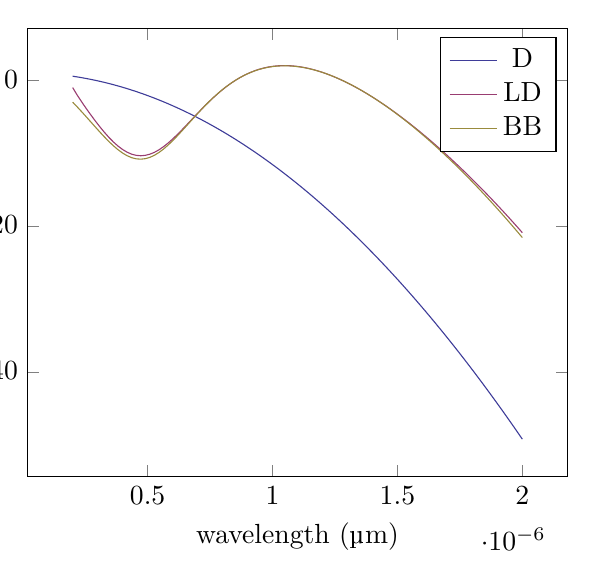
\begin{tikzpicture}[baseline,trim axis left]
\begin{axis}[xlabel=wavelength (\si{\micro\meter}),ylabel=$\epsilon'$]
\addplot[color=colora] coordinates {
(2e-07, 0.494840412391)
(2.18181818182e-07, 0.398824910147)
(2.36363636364e-07, 0.294462613359)
(2.54545454545e-07, 0.18175411682)
(2.72727272727e-07, 0.0607000628659)
(2.90909090909e-07, -0.0686988586329)
(3.09090909091e-07, -0.206441910281)
(3.27272727273e-07, -0.35252830717)
(3.45454545455e-07, -0.506957216888)
(3.63636363636e-07, -0.669727759529)
(3.81818181818e-07, -0.840839007713)
(4e-07, -1.02028998659)
(4.18181818182e-07, -1.20807967387)
(4.36363636364e-07, -1.4042069998)
(4.54545454545e-07, -1.60867084724)
(4.72727272727e-07, -1.82147005161)
(4.90909090909e-07, -2.04260340097)
(5.09090909091e-07, -2.27206963598)
(5.27272727273e-07, -2.50986744998)
(5.45454545455e-07, -2.75599548894)
(5.63636363636e-07, -3.01045235154)
(5.81818181818e-07, -3.27323658914)
(6e-07, -3.54434670584)
(6.18181818182e-07, -3.82378115849)
(6.36363636364e-07, -4.1115383567)
(6.54545454545e-07, -4.40761666286)
(6.72727272727e-07, -4.71201439219)
(6.90909090909e-07, -5.02472981273)
(7.09090909091e-07, -5.34576114541)
(7.27272727273e-07, -5.67510656402)
(7.45454545455e-07, -6.01276419528)
(7.63636363636e-07, -6.35873211883)
(7.81818181818e-07, -6.7130083673)
(8e-07, -7.0755909263)
(8.18181818182e-07, -7.44647773447)
(8.36363636364e-07, -7.8256666835)
(8.54545454545e-07, -8.21315561817)
(8.72727272727e-07, -8.60894233636)
(8.90909090909e-07, -9.0130245891)
(9.09090909091e-07, -9.42540008061)
(9.27272727273e-07, -9.84606646829)
(9.45454545455e-07, -10.2750213628)
(9.63636363636e-07, -10.7122623281)
(9.81818181818e-07, -11.1577868815)
(1e-06, -11.6115924934)
(1.01818181818e-06, -12.0736765879)
(1.03636363636e-06, -12.5440365424)
(1.05454545455e-06, -13.0226696878)
(1.07272727273e-06, -13.5095733083)
(1.09090909091e-06, -14.0047446419)
(1.10909090909e-06, -14.5081808799)
(1.12727272727e-06, -15.0198791675)
(1.14545454545e-06, -15.5398366034)
(1.16363636364e-06, -16.0680502398)
(1.18181818182e-06, -16.6045170831)
(1.2e-06, -17.149234093)
(1.21818181818e-06, -17.7021981833)
(1.23636363636e-06, -18.2634062217)
(1.25454545455e-06, -18.8328550295)
(1.27272727273e-06, -19.4105413822)
(1.29090909091e-06, -19.9964620093)
(1.30909090909e-06, -20.5906135942)
(1.32727272727e-06, -21.1929927746)
(1.34545454545e-06, -21.8035961421)
(1.36363636364e-06, -22.4224202426)
(1.38181818182e-06, -23.0494615763)
(1.4e-06, -23.6847165976)
(1.41818181818e-06, -24.3281817152)
(1.43636363636e-06, -24.9798532922)
(1.45454545455e-06, -25.6397276463)
(1.47272727273e-06, -26.3078010495)
(1.49090909091e-06, -26.9840697283)
(1.50909090909e-06, -27.668529864)
(1.52727272727e-06, -28.3611775924)
(1.54545454545e-06, -29.062009004)
(1.56363636364e-06, -29.7710201441)
(1.58181818182e-06, -30.4882070129)
(1.6e-06, -31.2135655651)
(1.61818181818e-06, -31.9470917109)
(1.63636363636e-06, -32.688781315)
(1.65454545455e-06, -33.4386301973)
(1.67272727273e-06, -34.1966341328)
(1.69090909091e-06, -34.9627888518)
(1.70909090909e-06, -35.7370900395)
(1.72727272727e-06, -36.5195333367)
(1.74545454545e-06, -37.3101143393)
(1.76363636364e-06, -38.1088285987)
(1.78181818182e-06, -38.9156716219)
(1.8e-06, -39.7306388711)
(1.81818181818e-06, -40.5537257643)
(1.83636363636e-06, -41.3849276752)
(1.85454545455e-06, -42.2242399331)
(1.87272727273e-06, -43.0716578231)
(1.89090909091e-06, -43.9271765862)
(1.90909090909e-06, -44.7907914192)
(1.92727272727e-06, -45.6624974751)
(1.94545454545e-06, -46.5422898628)
(1.96363636364e-06, -47.4301636472)
(1.98181818182e-06, -48.3261138496)
(2e-06, -49.2301354474)
};
\addlegendentry{D}
\addplot[color=colorb] coordinates {
(2e-07, -1.06008791576)
(2.18181818182e-07, -2.08728691496)
(2.36363636364e-07, -3.03312729992)
(2.54545454545e-07, -3.93493541402)
(2.72727272727e-07, -4.80459662206)
(2.90909090909e-07, -5.64246508885)
(3.09090909091e-07, -6.44304945983)
(3.27272727273e-07, -7.19771788561)
(3.45454545455e-07, -7.89621925268)
(3.63636363636e-07, -8.52770014973)
(3.81818181818e-07, -9.08149122815)
(4e-07, -9.54777117235)
(4.18181818182e-07, -9.91814198164)
(4.36363636364e-07, -10.1861139301)
(4.54545454545e-07, -10.3474831503)
(4.72727272727e-07, -10.4005814192)
(4.90909090909e-07, -10.3463824614)
(5.09090909091e-07, -10.1884590831)
(5.27272727273e-07, -9.93279802239)
(5.45454545455e-07, -9.58749193181)
(5.63636363636e-07, -9.16233809989)
(5.81818181818e-07, -8.66837976927)
(6e-07, -8.11742751865)
(6.18181818182e-07, -7.52159538895)
(6.36363636364e-07, -6.89288022851)
(6.54545454545e-07, -6.24280450264)
(6.72727272727e-07, -5.58213401409)
(6.90909090909e-07, -4.92067383948)
(7.09090909091e-07, -4.26713913845)
(7.27272727273e-07, -3.62909274225)
(7.45454545455e-07, -3.01293860584)
(7.63636363636e-07, -2.42395907891)
(7.81818181818e-07, -1.8663841388)
(8e-07, -1.34348181382)
(8.18181818182e-07, -0.857660625871)
(8.36363636364e-07, -0.410576683105)
(8.54545454545e-07, -0.00323983237963)
(8.72727272727e-07, 0.363885105257)
(8.90909090909e-07, 0.690784621335)
(9.09090909091e-07, 0.977811828695)
(9.27272727273e-07, 1.22561144441)
(9.45454545455e-07, 1.4350544817)
(9.63636363636e-07, 1.60718226149)
(9.81818181818e-07, 1.74315908478)
(1e-06, 1.84423275573)
(1.01818181818e-06, 1.91170208112)
(1.03636363636e-06, 1.94689046824)
(1.05454545455e-06, 1.95112477999)
(1.07272727273e-06, 1.92571866714)
(1.09090909091e-06, 1.87195967221)
(1.10909090909e-06, 1.79109947885)
(1.12727272727e-06, 1.68434675945)
(1.14545454545e-06, 1.55286214912)
(1.16363636364e-06, 1.39775494311)
(1.18181818182e-06, 1.22008117712)
(1.2e-06, 1.02084280507)
(1.21818181818e-06, 0.800987736806)
(1.23636363636e-06, 0.561410539417)
(1.25454545455e-06, 0.302953641309)
(1.27272727273e-06, 0.0264089077994)
(1.29090909091e-06, -0.267480517885)
(1.30909090909e-06, -0.578018193457)
(1.32727272727e-06, -0.904552244187)
(1.34545454545e-06, -1.2464731709)
(1.36363636364e-06, -1.60321164122)
(1.38181818182e-06, -1.97423629635)
(1.4e-06, -2.3590515979)
(1.41818181818e-06, -2.75719573285)
(1.43636363636e-06, -3.16823858988)
(1.45454545455e-06, -3.59177981611)
(1.47272727273e-06, -4.02744695995)
(1.49090909091e-06, -4.47489370364)
(1.50909090909e-06, -4.93379818658)
(1.52727272727e-06, -5.40386141943)
(1.54545454545e-06, -5.88480578758)
(1.56363636364e-06, -6.3763736418)
(1.58181818182e-06, -6.87832597332)
(1.6e-06, -7.39044116997)
(1.61818181818e-06, -7.91251384995)
(1.63636363636e-06, -8.44435376946)
(1.65454545455e-06, -8.98578480039)
(1.67272727273e-06, -9.5366439743)
(1.69090909091e-06, -10.096780589)
(1.70909090909e-06, -10.6660553736)
(1.72727272727e-06, -11.2443397097)
(1.74545454545e-06, -11.8315149033)
(1.76363636364e-06, -12.4274715062)
(1.78181818182e-06, -13.0321086826)
(1.8e-06, -13.6453336178)
(1.81818181818e-06, -14.2670609673)
(1.83636363636e-06, -14.8972123425)
(1.85454545455e-06, -15.5357158311)
(1.87272727273e-06, -16.1825055496)
(1.89090909091e-06, -16.8375212262)
(1.90909090909e-06, -17.5007078116)
(1.92727272727e-06, -18.1720151155)
(1.94545454545e-06, -18.8513974681)
(1.96363636364e-06, -19.5388134038)
(1.98181818182e-06, -20.2342253662)
(2e-06, -20.9375994327)
};
\addlegendentry{LD}
\addplot[color=colorc] coordinates {
(2e-07, -3.05828291357)
(2.18181818182e-07, -3.70667385247)
(2.36363636364e-07, -4.37922965836)
(2.54545454545e-07, -5.06897729931)
(2.72727272727e-07, -5.76807943186)
(2.90909090909e-07, -6.46765429841)
(3.09090909091e-07, -7.1576360649)
(3.27272727273e-07, -7.82671548312)
(3.45454545455e-07, -8.46240330112)
(3.63636363636e-07, -9.05125744467)
(3.81818181818e-07, -9.57930449225)
(4e-07, -10.0326616949)
(4.18181818182e-07, -10.3983276881)
(4.36363636364e-07, -10.6650650316)
(4.54545454545e-07, -10.8242598597)
(4.72727272727e-07, -10.8706290015)
(4.90909090909e-07, -10.8026621103)
(5.09090909091e-07, -10.6227324814)
(5.27272727273e-07, -10.336870963)
(5.45454545455e-07, -9.95425417557)
(5.63636363636e-07, -9.48649666172)
(5.81818181818e-07, -8.94685070944)
(6e-07, -8.34940995837)
(6.18181818182e-07, -7.70839102039)
(6.36363636364e-07, -7.03753982044)
(6.54545454545e-07, -6.34968308167)
(6.72727272727e-07, -5.65642444286)
(6.90909090909e-07, -4.96797058106)
(7.09090909091e-07, -4.29306504977)
(7.27272727273e-07, -3.63900500032)
(7.45454545455e-07, -3.01171691748)
(7.63636363636e-07, -2.41587049775)
(7.81818181818e-07, -1.85501368751)
(8e-07, -1.3317158998)
(8.18181818182e-07, -0.847710081441)
(8.36363636364e-07, -0.404027383045)
(8.54545454545e-07, -0.00112063032229)
(8.72727272727e-07, 0.361025362361)
(8.90909090909e-07, 0.68279727555)
(9.09090909091e-07, 0.964870310723)
(9.27272727273e-07, 1.20813793974)
(9.45454545455e-07, 1.41365323862)
(9.63636363636e-07, 1.58258052048)
(9.81818181818e-07, 1.71615595405)
(1e-06, 1.81565590219)
(1.01818181818e-06, 1.88237180709)
(1.03636363636e-06, 1.91759056509)
(1.05454545455e-06, 1.92257945818)
(1.07272727273e-06, 1.89857483251)
(1.09090909091e-06, 1.84677383082)
(1.10909090909e-06, 1.76832859145)
(1.12727272727e-06, 1.66434242168)
(1.14545454545e-06, 1.53586753556)
(1.16363636364e-06, 1.38390401813)
(1.18181818182e-06, 1.20939973852)
(1.2e-06, 1.01325098614)
(1.21818181818e-06, 0.796303646938)
(1.23636363636e-06, 0.559354772825)
(1.25454545455e-06, 0.303154426784)
(1.27272727273e-06, 0.0284077106843)
(1.29090909091e-06, -0.264223097332)
(1.30909090909e-06, -0.574116352752)
(1.32727272727e-06, -0.900688845626)
(1.34545454545e-06, -1.24339362565)
(1.36363636364e-06, -1.60171787607)
(1.38181818182e-06, -1.97518085415)
(1.4e-06, -2.36333191087)
(1.41818181818e-06, -2.76574859789)
(1.43636363636e-06, -3.18203486678)
(1.45454545455e-06, -3.61181936294)
(1.47272727273e-06, -4.05475381452)
(1.49090909091e-06, -4.51051151522)
(1.50909090909e-06, -4.97878589902)
(1.52727272727e-06, -5.45928920354)
(1.54545454545e-06, -5.9517512188)
(1.56363636364e-06, -6.45591811736)
(1.58181818182e-06, -6.97155136179)
(1.6e-06, -7.49842668533)
(1.61818181818e-06, -8.03633314145)
(1.63636363636e-06, -8.5850722183)
(1.65454545455e-06, -9.14445701391)
(1.67272727273e-06, -9.71431146827)
(1.69090909091e-06, -10.2944696486)
(1.70909090909e-06, -10.8847750842)
(1.72727272727e-06, -11.4850801475)
(1.74545454545e-06, -12.095245478)
(1.76363636364e-06, -12.7151394467)
(1.78181818182e-06, -13.3446376569)
(1.8e-06, -13.9836224806)
(1.81818181818e-06, -14.6319826259)
(1.83636363636e-06, -15.289612735)
(1.85454545455e-06, -15.9564130099)
(1.87272727273e-06, -16.6322888627)
(1.89090909091e-06, -17.3171505914)
(1.90909090909e-06, -18.0109130761)
(1.92727272727e-06, -18.7134954969)
(1.94545454545e-06, -19.4248210706)
(1.96363636364e-06, -20.1448168044)
(1.98181818182e-06, -20.8734132668)
(2e-06, -21.6105443735)
};
\addlegendentry{BB}
\end{axis}
\end{tikzpicture}%
\\
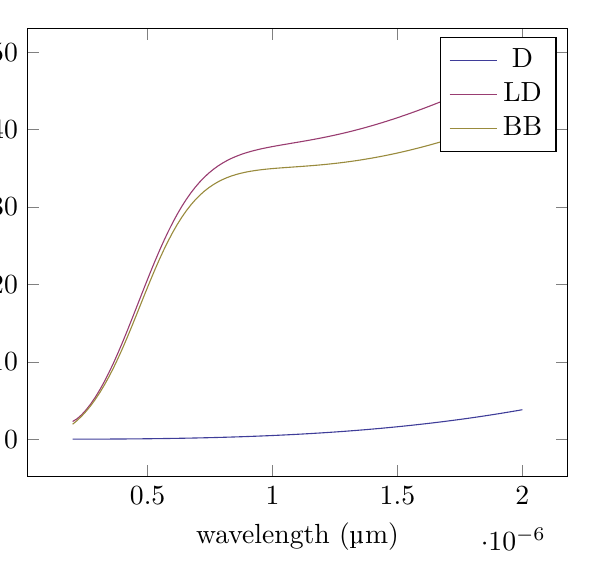
\begin{tikzpicture}[baseline,trim axis left]
\begin{axis}[xlabel=wavelength (\si{\micro\meter}),ylabel=$\epsilon''$]
\addplot[color=colora] coordinates {
(2e-07, 0.00382992380858)
(2.18181818182e-07, 0.00497222842675)
(2.36363636364e-07, 0.00632167600027)
(2.54545454545e-07, 0.00789551955927)
(2.72727272727e-07, 0.00971101000251)
(2.90909090909e-07, 0.0117853959336)
(3.09090909091e-07, 0.0141359234976)
(3.27272727273e-07, 0.0167798362168)
(3.45454545455e-07, 0.0197343748276)
(3.63636363636e-07, 0.023016777117)
(3.81818181818e-07, 0.0266442777586)
(4e-07, 0.0306341081499)
(4.18181818182e-07, 0.0350034962483)
(4.36363636364e-07, 0.0397696664082)
(4.54545454545e-07, 0.0449498392176)
(4.72727272727e-07, 0.0505612313351)
(4.90909090909e-07, 0.0566210553267)
(5.09090909091e-07, 0.0631465195029)
(5.27272727273e-07, 0.0701548277559)
(5.45454545455e-07, 0.0776631793967)
(5.63636363636e-07, 0.0856887689921)
(5.81818181818e-07, 0.0942487862026)
(6e-07, 0.10336041562)
(6.18181818182e-07, 0.113040836603)
(6.36363636364e-07, 0.123307223119)
(6.54545454545e-07, 0.134176743577)
(6.72727272727e-07, 0.145666560669)
(6.90909090909e-07, 0.157793831208)
(7.09090909091e-07, 0.170575705963)
(7.27272727273e-07, 0.184029329499)
(7.45454545455e-07, 0.198171840019)
(7.63636363636e-07, 0.213020369195)
(7.81818181818e-07, 0.228592042013)
(8e-07, 0.24490397661)
(8.18181818182e-07, 0.261973284111)
(8.36363636364e-07, 0.27981706847)
(8.54545454545e-07, 0.298452426309)
(8.72727272727e-07, 0.317896446757)
(8.90909090909e-07, 0.338166211289)
(9.09090909091e-07, 0.359278793565)
(9.27272727273e-07, 0.381251259275)
(9.45454545455e-07, 0.404100665969)
(9.63636363636e-07, 0.427844062907)
(9.81818181818e-07, 0.452498490895)
(1e-06, 0.478080982123)
(1.01818181818e-06, 0.504608560011)
(1.03636363636e-06, 0.532098239045)
(1.05454545455e-06, 0.560567024622)
(1.07272727273e-06, 0.590031912886)
(1.09090909091e-06, 0.620509890576)
(1.10909090909e-06, 0.652017934862)
(1.12727272727e-06, 0.684573013187)
(1.14545454545e-06, 0.718192083114)
(1.16363636364e-06, 0.752892092162)
(1.18181818182e-06, 0.788689977652)
(1.2e-06, 0.825602666548)
(1.21818181818e-06, 0.8636470753)
(1.23636363636e-06, 0.902840109686)
(1.25454545455e-06, 0.943198664658)
(1.27272727273e-06, 0.984739624182)
(1.29090909091e-06, 1.02747986108)
(1.30909090909e-06, 1.07143623689)
(1.32727272727e-06, 1.11662560167)
(1.34545454545e-06, 1.1630647939)
(1.36363636364e-06, 1.21077064027)
(1.38181818182e-06, 1.25975995557)
(1.4e-06, 1.3100495425)
(1.41818181818e-06, 1.36165619153)
(1.43636363636e-06, 1.41459668076)
(1.45454545455e-06, 1.46888777573)
(1.47272727273e-06, 1.52454622931)
(1.49090909091e-06, 1.5815887815)
(1.50909090909e-06, 1.64003215932)
(1.52727272727e-06, 1.69989307661)
(1.54545454545e-06, 1.76118823394)
(1.56363636364e-06, 1.82393431839)
(1.58181818182e-06, 1.88814800343)
(1.6e-06, 1.95384594878)
(1.61818181818e-06, 2.02104480023)
(1.63636363636e-06, 2.08976118951)
(1.65454545455e-06, 2.16001173412)
(1.67272727273e-06, 2.23181303719)
(1.69090909091e-06, 2.30518168734)
(1.70909090909e-06, 2.3801342585)
(1.72727272727e-06, 2.45668730978)
(1.74545454545e-06, 2.53485738534)
(1.76363636364e-06, 2.61466101418)
(1.78181818182e-06, 2.69611471005)
(1.8e-06, 2.77923497128)
(1.81818181818e-06, 2.86403828061)
(1.83636363636e-06, 2.95054110507)
(1.85454545455e-06, 3.03875989583)
(1.87272727273e-06, 3.12871108803)
(1.89090909091e-06, 3.22041110067)
(1.90909090909e-06, 3.31387633641)
(1.92727272727e-06, 3.40912318147)
(1.94545454545e-06, 3.50616800547)
(1.96363636364e-06, 3.60502716125)
(1.98181818182e-06, 3.70571698478)
(2e-06, 3.80825379498)
};
\addlegendentry{D}
\addplot[color=colorb] coordinates {
(2e-07, 2.28709502666)
(2.18181818182e-07, 2.65052155439)
(2.36363636364e-07, 3.172050902)
(2.54545454545e-07, 3.81724971338)
(2.72727272727e-07, 4.57373388372)
(2.90909090909e-07, 5.43585828401)
(3.09090909091e-07, 6.39971403342)
(3.27272727273e-07, 7.46111297871)
(3.45454545455e-07, 8.61464160238)
(3.63636363636e-07, 9.85318842692)
(3.81818181818e-07, 11.1677395742)
(4e-07, 12.5473671013)
(4.18181818182e-07, 13.9793786075)
(4.36363636364e-07, 15.4496077833)
(4.54545454545e-07, 16.942823271)
(4.72727272727e-07, 18.4432259275)
(4.90909090909e-07, 19.9349970382)
(5.09090909091e-07, 21.4028552149)
(5.27272727273e-07, 22.8325793176)
(5.45454545455e-07, 24.2114592903)
(5.63636363636e-07, 25.5286456774)
(5.81818181818e-07, 26.7753803088)
(6e-07, 27.9451032996)
(6.18181818182e-07, 29.0334431977)
(6.36363636364e-07, 30.0381063475)
(6.54545454545e-07, 30.9586875061)
(6.72727272727e-07, 31.7964262811)
(6.90909090909e-07, 32.5539334854)
(7.09090909091e-07, 33.2349087811)
(7.27272727273e-07, 33.8438668905)
(7.45454545455e-07, 34.3858850277)
(7.63636363636e-07, 34.8663796869)
(7.81818181818e-07, 35.290916967)
(8e-07, 35.6650574327)
(8.18181818182e-07, 35.9942341815)
(8.36363636364e-07, 36.2836612404)
(8.54545454545e-07, 36.5382685446)
(8.72727272727e-07, 36.762659396)
(8.90909090909e-07, 36.9610863223)
(9.09090909091e-07, 37.1374415291)
(9.27272727273e-07, 37.295258545)
(9.45454545455e-07, 37.4377221401)
(9.63636363636e-07, 37.5676840807)
(9.81818181818e-07, 37.6876827457)
(1e-06, 37.7999650411)
(1.01818181818e-06, 37.9065094116)
(1.03636363636e-06, 38.0090490472)
(1.05454545455e-06, 38.1090946336)
(1.07272727273e-06, 38.2079561904)
(1.09090909091e-06, 38.3067637006)
(1.10909090909e-06, 38.406486351)
(1.12727272727e-06, 38.5079502954)
(1.14545454545e-06, 38.6118549191)
(1.16363636364e-06, 38.718787628)
(1.18181818182e-06, 38.829237219)
(1.2e-06, 38.9436059103)
(1.21818181818e-06, 39.0622201207)
(1.23636363636e-06, 39.1853400942)
(1.25454545455e-06, 39.3131684673)
(1.27272727273e-06, 39.4458578754)
(1.29090909091e-06, 39.5835176897)
(1.30909090909e-06, 39.7262199721)
(1.32727272727e-06, 39.8740047285)
(1.34545454545e-06, 40.0268845359)
(1.36363636364e-06, 40.1848486109)
(1.38181818182e-06, 40.3478663817)
(1.4e-06, 40.51589062)
(1.41818181818e-06, 40.688860183)
(1.43636363636e-06, 40.8667024095)
(1.45454545455e-06, 41.0493352126)
(1.47272727273e-06, 41.2366689027)
(1.49090909091e-06, 41.4286077737)
(1.50909090909e-06, 41.6250514812)
(1.52727272727e-06, 41.8258962359)
(1.54545454545e-06, 42.0310358368)
(1.56363636364e-06, 42.2403625619)
(1.58181818182e-06, 42.4537679344)
(1.6e-06, 42.6711433799)
(1.61818181818e-06, 42.8923807875)
(1.63636363636e-06, 43.1173729871)
(1.65454545455e-06, 43.3460141532)
(1.67272727273e-06, 43.5782001442)
(1.69090909091e-06, 43.8138287857)
(1.70909090909e-06, 44.0528001046)
(1.72727272727e-06, 44.2950165203)
(1.74545454545e-06, 44.540382999)
(1.76363636364e-06, 44.7888071748)
(1.78181818182e-06, 45.0401994433)
(1.8e-06, 45.2944730303)
(1.81818181818e-06, 45.5515440396)
(1.83636363636e-06, 45.8113314827)
(1.85454545455e-06, 46.0737572918)
(1.87272727273e-06, 46.3387463207)
(1.89090909091e-06, 46.6062263332)
(1.90909090909e-06, 46.8761279819)
(1.92727272727e-06, 47.1483847787)
(1.94545454545e-06, 47.4229330582)
(1.96363636364e-06, 47.6997119357)
(1.98181818182e-06, 47.9786632593)
(2e-06, 48.2597315596)
};
\addlegendentry{LD}
\addplot[color=colorc] coordinates {
(2e-07, 1.93511846844)
(2.18181818182e-07, 2.4265077183)
(2.36363636364e-07, 2.98977526199)
(2.54545454545e-07, 3.6290377371)
(2.72727272727e-07, 4.34815527758)
(2.90909090909e-07, 5.15054523795)
(3.09090909091e-07, 6.03889389177)
(3.27272727273e-07, 7.01477363421)
(3.45454545455e-07, 8.07818581532)
(3.63636363636e-07, 9.22706757387)
(3.81818181818e-07, 10.4568233169)
(4e-07, 11.7599618086)
(4.18181818182e-07, 13.1259287839)
(4.36363636364e-07, 14.5412127081)
(4.54545454545e-07, 15.9897635342)
(4.72727272727e-07, 17.4537073588)
(4.90909090909e-07, 18.9142799842)
(5.09090909091e-07, 20.3528588289)
(5.27272727273e-07, 21.7519585074)
(5.45454545455e-07, 23.0960722987)
(5.63636363636e-07, 24.3722806753)
(5.81818181818e-07, 25.5705951807)
(6e-07, 26.684048495)
(6.18181818182e-07, 27.7085716932)
(6.36363636364e-07, 28.6427152133)
(6.54545454545e-07, 29.4872727482)
(6.72727272727e-07, 30.2448610524)
(6.90909090909e-07, 30.91949766)
(7.09090909091e-07, 31.5162061508)
(7.27272727273e-07, 32.0406671233)
(7.45454545455e-07, 32.4989236224)
(7.63636363636e-07, 32.8971428031)
(7.81818181818e-07, 33.2414309463)
(8e-07, 33.5376962037)
(8.18181818182e-07, 33.7915521551)
(8.36363636364e-07, 34.0082549818)
(8.54545454545e-07, 34.1926674179)
(8.72727272727e-07, 34.3492433546)
(8.90909090909e-07, 34.4820278498)
(9.09090909091e-07, 34.5946681942)
(9.27272727273e-07, 34.6904325357)
(9.45454545455e-07, 34.7722333206)
(9.63636363636e-07, 34.8426534548)
(9.81818181818e-07, 34.903973626)
(1e-06, 34.9581996588)
(1.01818181818e-06, 35.0070891134)
(1.03636363636e-06, 35.0521766075)
(1.05454545455e-06, 35.0947975342)
(1.07272727273e-06, 35.1361100031)
(1.09090909091e-06, 35.1771149351)
(1.10909090909e-06, 35.2186743184)
(1.12727272727e-06, 35.2615276867)
(1.14545454545e-06, 35.3063069107)
(1.16363636364e-06, 35.353549416)
(1.18181818182e-06, 35.4037099514)
(1.2e-06, 35.4571710307)
(1.21818181818e-06, 35.5142521749)
(1.23636363636e-06, 35.5752180719)
(1.25454545455e-06, 35.6402857669)
(1.27272727273e-06, 35.709630988)
(1.29090909091e-06, 35.7833937019)
(1.30909090909e-06, 35.8616829869)
(1.32727272727e-06, 35.9445813032)
(1.34545454545e-06, 36.0321482297)
(1.36363636364e-06, 36.1244237306)
(1.38181818182e-06, 36.22143101)
(1.4e-06, 36.3231790018)
(1.41818181818e-06, 36.4296645414)
(1.43636363636e-06, 36.5408742572)
(1.45454545455e-06, 36.6567862167)
(1.47272727273e-06, 36.7773713581)
(1.49090909091e-06, 36.9025947326)
(1.50909090909e-06, 37.0324165836)
(1.52727272727e-06, 37.16679328)
(1.54545454545e-06, 37.305678125)
(1.56363636364e-06, 37.4490220537)
(1.58181818182e-06, 37.5967742354)
(1.6e-06, 37.7488825906)
(1.61818181818e-06, 37.9052942363)
(1.63636363636e-06, 38.0659558655)
(1.65454545455e-06, 38.2308140723)
(1.67272727273e-06, 38.399815627)
(1.69090909091e-06, 38.5729077103)
(1.70909090909e-06, 38.7500381088)
(1.72727272727e-06, 38.9311553798)
(1.74545454545e-06, 39.1162089872)
(1.76363636364e-06, 39.305149414)
(1.78181818182e-06, 39.4979282526)
(1.8e-06, 39.6944982778)
(1.81818181818e-06, 39.8948135037)
(1.83636363636e-06, 40.0988292268)
(1.85454545455e-06, 40.3065020578)
(1.87272727273e-06, 40.5177899423)
(1.89090909091e-06, 40.7326521741)
(1.90909090909e-06, 40.9510494003)
(1.92727272727e-06, 41.1729436201)
(1.94545454545e-06, 41.3982981783)
(1.96363636364e-06, 41.6270777546)
(1.98181818182e-06, 41.8592483487)
(2e-06, 42.0947772621)
};
\addlegendentry{BB}
\end{axis}
\end{tikzpicture}%
\\
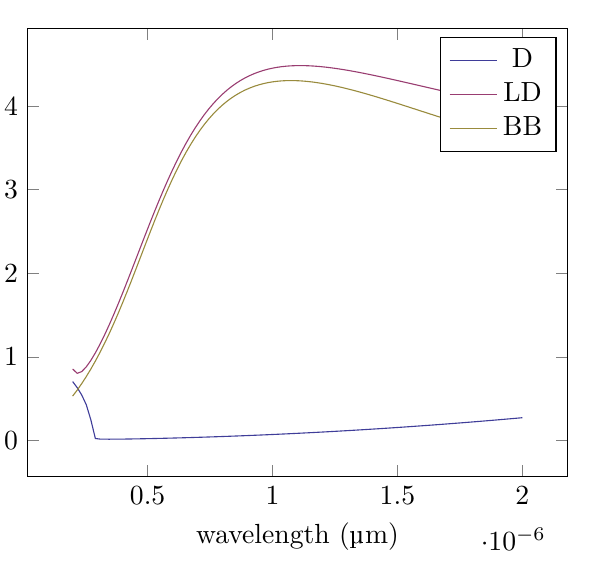
\begin{tikzpicture}[baseline,trim axis left]
\begin{axis}[xlabel=wavelength (\si{\micro\meter}),ylabel=$n'$]
\addplot[color=colora] coordinates {
(2e-07, 0.703454208112)
(2.18181818182e-07, 0.631538127892)
(2.36363636364e-07, 0.542675352955)
(2.54545454545e-07, 0.42642680856)
(2.72727272727e-07, 0.247155840154)
(2.90909090909e-07, 0.0224005722351)
(3.09090909091e-07, 0.0155468055829)
(3.27272727273e-07, 0.0141266060798)
(3.45454545455e-07, 0.0138556054202)
(3.63636363636e-07, 0.0140605165451)
(3.81818181818e-07, 0.0145265686786)
(4e-07, 0.0151622799374)
(4.18181818182e-07, 0.0159216502721)
(4.36363636364e-07, 0.016778875592)
(4.54545454545e-07, 0.0177183052018)
(4.72727272727e-07, 0.0187298720708)
(4.90909090909e-07, 0.0198067963675)
(5.09090909091e-07, 0.0209443401914)
(5.27272727273e-07, 0.0221390903389)
(5.45454545455e-07, 0.0233885244081)
(5.63636363636e-07, 0.0246907373841)
(5.81818181818e-07, 0.026044263305)
(6e-07, 0.0274479554596)
(6.18181818182e-07, 0.0289009038204)
(6.36363636364e-07, 0.0304023768496)
(6.54545454545e-07, 0.0319517796652)
(6.72727272727e-07, 0.0335486234333)
(6.90909090909e-07, 0.0351925026205)
(7.09090909091e-07, 0.0368830778441)
(7.27272727273e-07, 0.0386200627779)
(7.45454545455e-07, 0.0404032140349)
(7.63636363636e-07, 0.0422323232677)
(7.81818181818e-07, 0.044107210939)
(8e-07, 0.0460277213649)
(8.18181818182e-07, 0.0479937187376)
(8.36363636364e-07, 0.0500050839099)
(8.54545454545e-07, 0.0520617117763)
(8.72727272727e-07, 0.0541635091255)
(8.90909090909e-07, 0.0563103928694)
(9.09090909091e-07, 0.0585022885726)
(9.27272727273e-07, 0.0607391292265)
(9.45454545455e-07, 0.06302085422)
(9.63636363636e-07, 0.0653474084725)
(9.81818181818e-07, 0.0677187417001)
(1e-06, 0.0701348077911)
(1.01818181818e-06, 0.0725955642731)
(1.03636363636e-06, 0.075100971856)
(1.05454545455e-06, 0.0776509940388)
(1.07272727273e-06, 0.0802455967706)
(1.09090909091e-06, 0.0828847481562)
(1.10909090909e-06, 0.0855684182007)
(1.12727272727e-06, 0.088296578587)
(1.14545454545e-06, 0.0910692024808)
(1.16363636364e-06, 0.0938862643601)
(1.18181818182e-06, 0.0967477398652)
(1.2e-06, 0.0996536056665)
(1.21818181818e-06, 0.102603839347)
(1.23636363636e-06, 0.105598419302)
(1.25454545455e-06, 0.108637324641)
(1.27272727273e-06, 0.111720535113)
(1.29090909091e-06, 0.114848031029)
(1.30909090909e-06, 0.118019793202)
(1.32727272727e-06, 0.121235802882)
(1.34545454545e-06, 0.12449604171)
(1.36363636364e-06, 0.127800491667)
(1.38181818182e-06, 0.131149135037)
(1.4e-06, 0.134541954364)
(1.41818181818e-06, 0.137978932419)
(1.43636363636e-06, 0.141460052173)
(1.45454545455e-06, 0.144985296762)
(1.47272727273e-06, 0.148554649468)
(1.49090909091e-06, 0.152168093695)
(1.50909090909e-06, 0.155825612943)
(1.52727272727e-06, 0.159527190797)
(1.54545454545e-06, 0.163272810901)
(1.56363636364e-06, 0.16706245695)
(1.58181818182e-06, 0.170896112671)
(1.6e-06, 0.17477376181)
(1.61818181818e-06, 0.178695388121)
(1.63636363636e-06, 0.182660975356)
(1.65454545455e-06, 0.186670507254)
(1.67272727273e-06, 0.190723967527)
(1.69090909091e-06, 0.194821339862)
(1.70909090909e-06, 0.198962607901)
(1.72727272727e-06, 0.203147755244)
(1.74545454545e-06, 0.207376765435)
(1.76363636364e-06, 0.211649621959)
(1.78181818182e-06, 0.215966308237)
(1.8e-06, 0.22032680762)
(1.81818181818e-06, 0.224731103383)
(1.83636363636e-06, 0.229179178722)
(1.85454545455e-06, 0.233671016748)
(1.87272727273e-06, 0.238206600486)
(1.89090909091e-06, 0.242785912869)
(1.90909090909e-06, 0.247408936737)
(1.92727272727e-06, 0.252075654829)
(1.94545454545e-06, 0.256786049789)
(1.96363636364e-06, 0.261540104153)
(1.98181818182e-06, 0.266337800355)
(2e-06, 0.27117912072)
};
\addlegendentry{D}
\addplot[color=colorb] coordinates {
(2e-07, 0.85461784041)
(2.18181818182e-07, 0.802009877012)
(2.36363636364e-07, 0.823315186657)
(2.54545454545e-07, 0.879579125139)
(2.72727272727e-07, 0.956267074411)
(2.90909090909e-07, 1.04700875494)
(3.09090909091e-07, 1.14852239733)
(3.27272727273e-07, 1.25883159658)
(3.45454545455e-07, 1.37654809192)
(3.63636363636e-07, 1.50055007256)
(3.81818181818e-07, 1.62982674537)
(4e-07, 1.76340119001)
(4.18181818182e-07, 1.90029422331)
(4.36363636364e-07, 2.03951191105)
(4.54545454545e-07, 2.18004771857)
(4.72727272727e-07, 2.32089394856)
(4.90909090909e-07, 2.46105877494)
(5.09090909091e-07, 2.59958600251)
(5.27272727273e-07, 2.73557518955)
(5.45454545455e-07, 2.86820020408)
(5.63636363636e-07, 2.99672473882)
(5.81818181818e-07, 3.12051379787)
(6e-07, 3.23904066331)
(6.18181818182e-07, 3.35188930863)
(6.36363636364e-07, 3.45875260731)
(6.54545454545e-07, 3.55942696239)
(6.72727272727e-07, 3.65380414585)
(6.90909090909e-07, 3.74186119324)
(7.09090909091e-07, 3.82364916754)
(7.27272727273e-07, 3.8992815123)
(7.45454545455e-07, 3.96892258361)
(7.63636363636e-07, 4.03277680649)
(7.81818181818e-07, 4.09107876146)
(8e-07, 4.14408438229)
(8.18181818182e-07, 4.19206334371)
(8.36363636364e-07, 4.23529263886)
(8.54545454545e-07, 4.27405128981)
(8.72727272727e-07, 4.30861609833)
(8.90909090909e-07, 4.33925832334)
(9.09090909091e-07, 4.36624116354)
(9.27272727273e-07, 4.38981792435)
(9.45454545455e-07, 4.41023075482)
(9.63636363636e-07, 4.42770985053)
(9.81818181818e-07, 4.4424730301)
(1e-06, 4.45472560557)
(1.01818181818e-06, 4.46466047898)
(1.03636363636e-06, 4.47245840861)
(1.05454545455e-06, 4.47828839856)
(1.07272727273e-06, 4.48230817422)
(1.09090909091e-06, 4.4846647137)
(1.10909090909e-06, 4.4854948117)
(1.12727272727e-06, 4.48492565787)
(1.14545454545e-06, 4.48307541567)
(1.16363636364e-06, 4.48005379177)
(1.18181818182e-06, 4.47596258853)
(1.2e-06, 4.47089623444)
(1.21818181818e-06, 4.46494228936)
(1.23636363636e-06, 4.45818192244)
(1.25454545455e-06, 4.45069036196)
(1.27272727273e-06, 4.44253731687)
(1.29090909091e-06, 4.43378737052)
(1.30909090909e-06, 4.42450034754)
(1.32727272727e-06, 4.41473165476)
(1.34545454545e-06, 4.40453259777)
(1.36363636364e-06, 4.39395067441)
(1.38181818182e-06, 4.38302984662)
(1.4e-06, 4.37181079221)
(1.41818181818e-06, 4.36033113794)
(1.43636363636e-06, 4.34862567535)
(1.45454545455e-06, 4.33672656059)
(1.47272727273e-06, 4.32466349959)
(1.49090909091e-06, 4.31246391964)
(1.50909090909e-06, 4.30015312856)
(1.52727272727e-06, 4.28775446245)
(1.54545454545e-06, 4.27528942283)
(1.56363636364e-06, 4.26277780424)
(1.58181818182e-06, 4.25023781278)
(1.6e-06, 4.23768617666)
(1.61818181818e-06, 4.22513824899)
(1.63636363636e-06, 4.21260810381)
(1.65454545455e-06, 4.20010862552)
(1.67272727273e-06, 4.18765159248)
(1.69090909091e-06, 4.17524775504)
(1.70909090909e-06, 4.16290690847)
(1.72727272727e-06, 4.15063796115)
(1.74545454545e-06, 4.13844899831)
(1.76363636364e-06, 4.12634734167)
(1.78181818182e-06, 4.11433960523)
(1.8e-06, 4.10243174745)
(1.81818181818e-06, 4.09062912006)
(1.83636363636e-06, 4.07893651373)
(1.85454545455e-06, 4.06735820077)
(1.87272727273e-06, 4.05589797504)
(1.89090909091e-06, 4.04455918927)
(1.90909090909e-06, 4.03334478991)
(1.92727272727e-06, 4.02225734966)
(1.94545454545e-06, 4.01129909789)
(1.96363636364e-06, 4.0004719489)
(1.98181818182e-06, 3.98977752838)
(2e-06, 3.97921719797)
};
\addlegendentry{LD}
\addplot[color=colorc] coordinates {
(2e-07, 0.529529183096)
(2.18181818182e-07, 0.601500209921)
(2.36363636364e-07, 0.679434001933)
(2.54545454545e-07, 0.763268703283)
(2.72727272727e-07, 0.85302371264)
(2.90909090909e-07, 0.948755979086)
(3.09090909091e-07, 1.05052163267)
(3.27272727273e-07, 1.15833824932)
(3.45454545455e-07, 1.27214669564)
(3.63636363636e-07, 1.39177368497)
(3.81818181818e-07, 1.51689795232)
(4e-07, 1.64702434146)
(4.18181818182e-07, 1.78147066642)
(4.36363636364e-07, 1.91937144828)
(4.54545454545e-07, 2.05970037801)
(4.72727272727e-07, 2.20131009321)
(4.90909090909e-07, 2.34298459322)
(5.09090909091e-07, 2.48349742603)
(5.27272727273e-07, 2.62166827927)
(5.45454545455e-07, 2.75641173156)
(5.63636363636e-07, 2.88677408178)
(5.81818181818e-07, 3.0119566145)
(6e-07, 3.13132576612)
(6.18181818182e-07, 3.24441210171)
(6.36363636364e-07, 3.35090074289)
(6.54545454545e-07, 3.45061602606)
(6.72727272727e-07, 3.5435029104)
(6.90909090909e-07, 3.62960718651)
(7.09090909091e-07, 3.70905600458)
(7.27272727273e-07, 3.78203974065)
(7.45454545455e-07, 3.84879579909)
(7.63636363636e-07, 3.90959462597)
(7.81818181818e-07, 3.96472797712)
(8e-07, 4.01449933357)
(8.18181818182e-07, 4.05921626792)
(8.36363636364e-07, 4.09918452208)
(8.54545454545e-07, 4.13470354475)
(8.72727272727e-07, 4.16606324548)
(8.90909090909e-07, 4.19354174188)
(9.09090909091e-07, 4.21740390255)
(9.27272727273e-07, 4.2379005157)
(9.45454545455e-07, 4.25526794042)
(9.63636363636e-07, 4.26972812242)
(9.81818181818e-07, 4.28148887807)
(1e-06, 4.29074436982)
(1.01818181818e-06, 4.29767571194)
(1.03636363636e-06, 4.30245165905)
(1.05454545455e-06, 4.30522934115)
(1.07272727273e-06, 4.30615501707)
(1.09090909091e-06, 4.30536482621)
(1.10909090909e-06, 4.30298552335)
(1.12727272727e-06, 4.29913518615)
(1.14545454545e-06, 4.2939238882)
(1.16363636364e-06, 4.28745433319)
(1.18181818182e-06, 4.27982244775)
(1.2e-06, 4.27111793189)
(1.21818181818e-06, 4.26142476731)
(1.23636363636e-06, 4.25082168437)
(1.25454545455e-06, 4.23938258938)
(1.27272727273e-06, 4.22717695384)
(1.29090909091e-06, 4.21427016798)
(1.30909090909e-06, 4.20072386068)
(1.32727272727e-06, 4.1865961882)
(1.34545454545e-06, 4.17194209393)
(1.36363636364e-06, 4.15681354156)
(1.38181818182e-06, 4.14125972387)
(1.4e-06, 4.12532724926)
(1.41818181818e-06, 4.10906030811)
(1.43636363636e-06, 4.09250082092)
(1.45454545455e-06, 4.07568857017)
(1.47272727273e-06, 4.05866131753)
(1.49090909091e-06, 4.04145490809)
(1.50909090909e-06, 4.02410336324)
(1.52727272727e-06, 4.00663896352)
(1.54545454545e-06, 3.98909232279)
(1.56363636364e-06, 3.97149245493)
(1.58181818182e-06, 3.95386683424)
(1.6e-06, 3.93624145041)
(1.61818181818e-06, 3.9186408591)
(1.63636363636e-06, 3.90108822891)
(1.65454545455e-06, 3.88360538536)
(1.67272727273e-06, 3.8662128527)
(1.69090909091e-06, 3.8489298939)
(1.70909090909e-06, 3.83177454936)
(1.72727272727e-06, 3.81476367481)
(1.74545454545e-06, 3.79791297857)
(1.76363636364e-06, 3.78123705845)
(1.78181818182e-06, 3.76474943865)
(1.8e-06, 3.74846260648)
(1.81818181818e-06, 3.73238804931)
(1.83636363636e-06, 3.71653629161)
(1.85454545455e-06, 3.70091693205)
(1.87272727273e-06, 3.68553868087)
(1.89090909091e-06, 3.67040939716)
(1.90909090909e-06, 3.65553612628)
(1.92727272727e-06, 3.64092513711)
(1.94545454545e-06, 3.62658195919)
(1.96363636364e-06, 3.61251141954)
(1.98181818182e-06, 3.59871767916)
(2e-06, 3.58520426901)
};
\addlegendentry{BB}
\end{axis}
\end{tikzpicture}%
\\
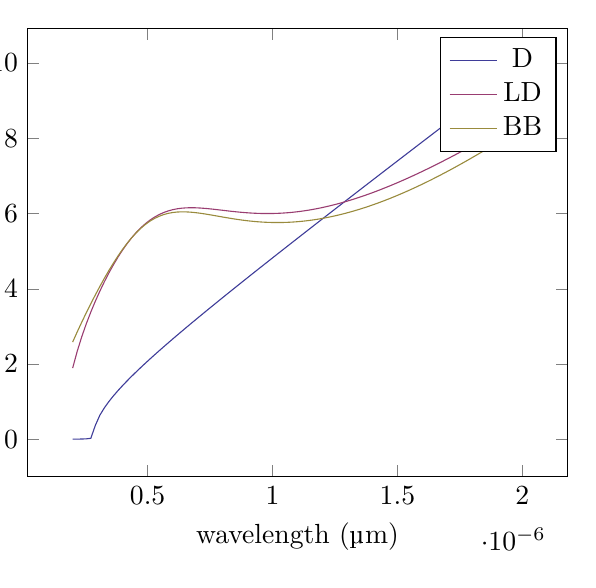
\begin{tikzpicture}[baseline,trim axis left]
\begin{axis}[xlabel=wavelength (\si{\micro\meter}),ylabel=$n''$]
\addplot[color=colora] coordinates {
(2e-07, 0.00384981007327)
(2.18181818182e-07, 0.00556719583962)
(2.36363636364e-07, 0.00823715310437)
(2.54545454545e-07, 0.0130924587978)
(2.72727272727e-07, 0.0277829608261)
(2.90909090909e-07, 0.372023236558)
(3.09090909091e-07, 0.642936409679)
(3.27272727273e-07, 0.839914124384)
(3.45454545455e-07, 1.00712382028)
(3.63636363636e-07, 1.15751929371)
(3.81818181818e-07, 1.29695800156)
(4e-07, 1.42864962907)
(4.18181818182e-07, 1.55456307226)
(4.36363636364e-07, 1.67600031651)
(4.54545454545e-07, 1.7938699984)
(4.72727272727e-07, 1.90883255406)
(4.90909090909e-07, 2.02138354112)
(5.09090909091e-07, 2.13190445441)
(5.27272727273e-07, 2.24069524447)
(5.45454545455e-07, 2.34799595912)
(5.63636363636e-07, 2.45400162349)
(5.81818181818e-07, 2.55887275682)
(6e-07, 2.66274298275)
(6.18181818182e-07, 2.76572465033)
(6.36363636364e-07, 2.86791306047)
(6.54545454545e-07, 2.96938969456)
(6.72727272727e-07, 3.07022471566)
(6.90909090909e-07, 3.17047893069)
(7.09090909091e-07, 3.27020534733)
(7.27272727273e-07, 3.36945042203)
(7.45454545455e-07, 3.46825506991)
(7.63636363636e-07, 3.56665548882)
(7.81818181818e-07, 3.66468383721)
(8e-07, 3.7623687957)
(8.18181818182e-07, 3.85973603541)
(8.36363636364e-07, 3.95680861097)
(8.54545454545e-07, 4.05360729228)
(8.72727272727e-07, 4.15015084595)
(8.90909090909e-07, 4.2464562754)
(9.09090909091e-07, 4.34253902651)
(9.27272727273e-07, 4.43841316466)
(9.45454545455e-07, 4.53409152772)
(9.63636363636e-07, 4.62958585878)
(9.81818181818e-07, 4.72490692171)
(1e-06, 4.82006460219)
(1.01818181818e-06, 4.91506799625)
(1.03636363636e-06, 5.00992548815)
(1.05454545455e-06, 5.10464481912)
(1.07272727273e-06, 5.19923314809)
(1.09090909091e-06, 5.29369710568)
(1.10909090909e-06, 5.38804284209)
(1.12727272727e-06, 5.4822760699)
(1.14545454545e-06, 5.57640210225)
(1.16363636364e-06, 5.67042588709)
(1.18181818182e-06, 5.76435203787)
(1.2e-06, 5.85818486122)
(1.21818181818e-06, 5.95192838183)
(1.23636363636e-06, 6.04558636491)
(1.25454545455e-06, 6.13916233663)
(1.27272727273e-06, 6.23265960247)
(1.29090909091e-06, 6.32608126402)
(1.30909090909e-06, 6.41943023418)
(1.32727272727e-06, 6.51270925107)
(1.34545454545e-06, 6.6059208906)
(1.36363636364e-06, 6.69906757814)
(1.38181818182e-06, 6.792151599)
(1.4e-06, 6.88517510817)
(1.41818181818e-06, 6.97814013917)
(1.43636363636e-06, 7.07104861228)
(1.45454545455e-06, 7.16390234196)
(1.47272727273e-06, 7.25670304386)
(1.49090909091e-06, 7.3494523411)
(1.50909090909e-06, 7.44215177025)
(1.52727272727e-06, 7.53480278667)
(1.54545454545e-06, 7.62740676964)
(1.56363636364e-06, 7.71996502695)
(1.58181818182e-06, 7.81247879923)
(1.6e-06, 7.90494926397)
(1.61818181818e-06, 7.99737753925)
(1.63636363636e-06, 8.08976468717)
(1.65454545455e-06, 8.1821117171)
(1.67272727273e-06, 8.27441958866)
(1.69090909091e-06, 8.36668921453)
(1.70909090909e-06, 8.45892146303)
(1.72727272727e-06, 8.5511171606)
(1.74545454545e-06, 8.64327709403)
(1.76363636364e-06, 8.73540201264)
(1.78181818182e-06, 8.8274926302)
(1.8e-06, 8.91954962688)
(1.81818181818e-06, 9.01157365093)
(1.83636363636e-06, 9.10356532037)
(1.85454545455e-06, 9.19552522449)
(1.87272727273e-06, 9.28745392533)
(1.89090909091e-06, 9.37935195903)
(1.90909090909e-06, 9.47121983709)
(1.92727272727e-06, 9.5630580476)
(1.94545454545e-06, 9.65486705637)
(1.96363636364e-06, 9.746647308)
(1.98181818182e-06, 9.83839922685)
(2e-06, 9.93012321806)
};
\addlegendentry{D}
\addplot[color=colorb] coordinates {
(2e-07, 1.89233166697)
(2.18181818182e-07, 2.33688115136)
(2.36363636364e-07, 2.72432567675)
(2.54545454545e-07, 3.06874399434)
(2.72727272727e-07, 3.38202405067)
(2.90909090909e-07, 3.67115579124)
(3.09090909091e-07, 3.94008963274)
(3.27272727273e-07, 4.19103206243)
(3.45454545455e-07, 4.42517884431)
(3.63636363636e-07, 4.64313486127)
(3.81818181818e-07, 4.84516799462)
(4e-07, 5.03137256209)
(4.18181818182e-07, 5.20178048687)
(4.36363636364e-07, 5.35643963196)
(4.54545454545e-07, 5.49546926214)
(4.72727272727e-07, 5.6190978172)
(4.90909090909e-07, 5.7276858774)
(5.09090909091e-07, 5.82173624747)
(5.27272727273e-07, 5.9018928557)
(5.45454545455e-07, 5.96893027978)
(5.63636363636e-07, 6.02373592717)
(5.81818181818e-07, 6.06728705963)
(6e-07, 6.10062487574)
(6.18181818182e-07, 6.12482772431)
(6.36363636364e-07, 6.14098523481)
(6.54545454545e-07, 6.15017476227)
(6.72727272727e-07, 6.15344111052)
(6.90909090909e-07, 6.15178007229)
(7.09090909091e-07, 6.14612594971)
(7.27272727273e-07, 6.13734291929)
(7.45454545455e-07, 6.12621989167)
(7.63636363636e-07, 6.11346838544)
(7.81818181818e-07, 6.09972287424)
(8e-07, 6.08554306226)
(8.18181818182e-07, 6.07141757806)
(8.36363636364e-07, 6.05776863538)
(8.54545454545e-07, 6.0449572803)
(8.72727272727e-07, 6.03328891692)
(8.90909090909e-07, 6.02301887351)
(9.09090909091e-07, 6.01435783264)
(9.27272727273e-07, 6.00747700196)
(9.45454545455e-07, 6.00251294527)
(9.63636363636e-07, 5.9995720279)
(9.81818181818e-07, 5.99873445626)
(1e-06, 6.00005791059)
(1.01818181818e-06, 6.00358078341)
(1.03636363636e-06, 6.00932504504)
(1.05454545455e-06, 6.01729876284)
(1.07272727273e-06, 6.02749830386)
(1.09090909091e-06, 6.03991025133)
(1.10909090909e-06, 6.05451306497)
(1.12727272727e-06, 6.07127851398)
(1.14545454545e-06, 6.09017290944)
(1.16363636364e-06, 6.11115816095)
(1.18181818182e-06, 6.13419267986)
(1.2e-06, 6.15923214923)
(1.21818181818e-06, 6.18623017847)
(1.23636363636e-06, 6.21513885833)
(1.25454545455e-06, 6.24590923033)
(1.27272727273e-06, 6.27849168255)
(1.29090909091e-06, 6.31283628251)
(1.30909090909e-06, 6.34889305609)
(1.32727272727e-06, 6.38661222053)
(1.34545454545e-06, 6.42594437818)
(1.36363636364e-06, 6.46684067693)
(1.38181818182e-06, 6.5092529422)
(1.4e-06, 6.55313378481)
(1.41818181818e-06, 6.59843668839)
(1.43636363636e-06, 6.64511607938)
(1.45454545455e-06, 6.69312738224)
(1.47272727273e-06, 6.74242706221)
(1.49090909091e-06, 6.79297265736)
(1.50909090909e-06, 6.84472280164)
(1.52727272727e-06, 6.89763724034)
(1.54545454545e-06, 6.95167683894)
(1.56363636364e-06, 7.00680358653)
(1.58181818182e-06, 7.06298059441)
(1.6e-06, 7.12017209087)
(1.61818181818e-06, 7.17834341238)
(1.63636363636e-06, 7.23746099205)
(1.65454545455e-06, 7.29749234553)
(1.67272727273e-06, 7.35840605489)
(1.69090909091e-06, 7.4201717507)
(1.70909090909e-06, 7.48276009267)
(1.72727272727e-06, 7.54614274901)
(1.74545454545e-06, 7.61029237479)
(1.76363636364e-06, 7.6751825894)
(1.78181818182e-06, 7.7407879534)
(1.8e-06, 7.80708394476)
(1.81818181818e-06, 7.87404693473)
(1.83636363636e-06, 7.94165416341)
(1.85454545455e-06, 8.00988371507)
(1.87272727273e-06, 8.07871449348)
(1.89090909091e-06, 8.14812619708)
(1.90909090909e-06, 8.21809929435)
(1.92727272727e-06, 8.28861499919)
(1.94545454545e-06, 8.35965524657)
(1.96363636364e-06, 8.43120266838)
(1.98181818182e-06, 8.50324056959)
(2e-06, 8.57575290471)
};
\addlegendentry{LD}
\addplot[color=colorc] coordinates {
(2e-07, 2.58406039764)
(2.18181818182e-07, 2.85253443625)
(2.36363636364e-07, 3.11154631055)
(2.54545454545e-07, 3.36201023577)
(2.72727272727e-07, 3.60436648697)
(2.90909090909e-07, 3.83869566553)
(3.09090909091e-07, 4.0647833314)
(3.27272727273e-07, 4.28216370144)
(3.45454545455e-07, 4.49015824139)
(3.63636363636e-07, 4.68791882072)
(3.81818181818e-07, 4.87448128317)
(4e-07, 5.04883172155)
(4.18181818182e-07, 5.20998376647)
(4.36363636364e-07, 5.35706109506)
(4.54545454545e-07, 5.48937619533)
(4.72727272727e-07, 5.60649536305)
(4.90909090909e-07, 5.70828151274)
(5.09090909091e-07, 5.79491017127)
(5.27272727273e-07, 5.86685870454)
(5.45454545455e-07, 5.92487296226)
(5.63636363636e-07, 5.9699181336)
(5.81818181818e-07, 6.00312141424)
(6e-07, 6.02571340373)
(6.18181818182e-07, 6.03897357274)
(6.36363636364e-07, 6.04418325486)
(6.54545454545e-07, 6.04258786299)
(6.72727272727e-07, 6.03536864141)
(6.90909090909e-07, 6.02362331316)
(7.09090909091e-07, 6.00835443277)
(7.27272727273e-07, 5.99046402212)
(7.45454545455e-07, 5.97075305478)
(7.63636363636e-07, 5.94992447636)
(7.81818181818e-07, 5.92858863813)
(8e-07, 5.90727023236)
(8.18181818182e-07, 5.88641602186)
(8.36363636364e-07, 5.86640283804)
(8.54545454545e-07, 5.84754547367)
(8.72727272727e-07, 5.83010421914)
(8.90909090909e-07, 5.81429188558)
(9.09090909091e-07, 5.80028022884)
(9.27272727273e-07, 5.78820573948)
(9.45454545455e-07, 5.77817479939)
(9.63636363636e-07, 5.77026822927)
(9.81818181818e-07, 5.76454526549)
(1e-06, 5.76104701335)
(1.01818181818e-06, 5.75979942669)
(1.03636363636e-06, 5.76081586468)
(1.05454545455e-06, 5.76409927425)
(1.07272727273e-06, 5.76964404422)
(1.09090909091e-06, 5.77743757317)
(1.10909090909e-06, 5.78746158912)
(1.12727272727e-06, 5.79969325519)
(1.14545454545e-06, 5.81410609158)
(1.16363636364e-06, 5.83067074034)
(1.18181818182e-06, 5.84935559627)
(1.2e-06, 5.87012732435)
(1.21818181818e-06, 5.89295128106)
(1.23636363636e-06, 5.91779185499)
(1.25454545455e-06, 5.94461273968)
(1.27272727273e-06, 5.97337715005)
(1.29090909091e-06, 6.00404799216)
(1.30909090909e-06, 6.0365879943)
(1.32727272727e-06, 6.07095980693)
(1.34545454545e-06, 6.10712607709)
(1.36363636364e-06, 6.1450495027)
(1.38181818182e-06, 6.18469287107)
(1.4e-06, 6.22601908516)
(1.41818181818e-06, 6.26899118097)
(1.43636363636e-06, 6.31357233838)
(1.45454545455e-06, 6.3597258878)
(1.47272727273e-06, 6.4074153143)
(1.49090909091e-06, 6.45660426065)
(1.50909090909e-06, 6.50725653053)
(1.52727272727e-06, 6.55933609255)
(1.54545454545e-06, 6.61280708603)
(1.56363636364e-06, 6.66763382872)
(1.58181818182e-06, 6.72378082699)
(1.6e-06, 6.78121278847)
(1.61818181818e-06, 6.83989463721)
(1.63636363636e-06, 6.89979153135)
(1.65454545455e-06, 6.96086888299)
(1.67272727273e-06, 7.02309238024)
(1.69090909091e-06, 7.08642801089)
(1.70909090909e-06, 7.15084208766)
(1.72727272727e-06, 7.21630127449)
(1.74545454545e-06, 7.28277261361)
(1.76363636364e-06, 7.35022355291)
(1.78181818182e-06, 7.41862197348)
(1.8e-06, 7.48793621671)
(1.81818181818e-06, 7.55813511079)
(1.83636363636e-06, 7.62918799635)
(1.85454545455e-06, 7.70106475077)
(1.87272727273e-06, 7.77373581116)
(1.89090909091e-06, 7.84717219565)
(1.90909090909e-06, 7.9213455229)
(1.92727272727e-06, 7.99622802964)
(1.94545454545e-06, 8.0717925862)
(1.96363636364e-06, 8.14801270995)
(1.98181818182e-06, 8.2248625765)
(2e-06, 8.30231702888)
};
\addlegendentry{BB}
\end{axis}
\end{tikzpicture}%
\\
\end{tabular}
\caption{Material parameters for Cr based on the Drude, Lorentz-Drude, and Brendel-Bormann models.}
\end{figure}
\clearpage
\newpage
\subsection{Ni}
\begin{figure}[h!]
\centering
\begin{tabular}{l}
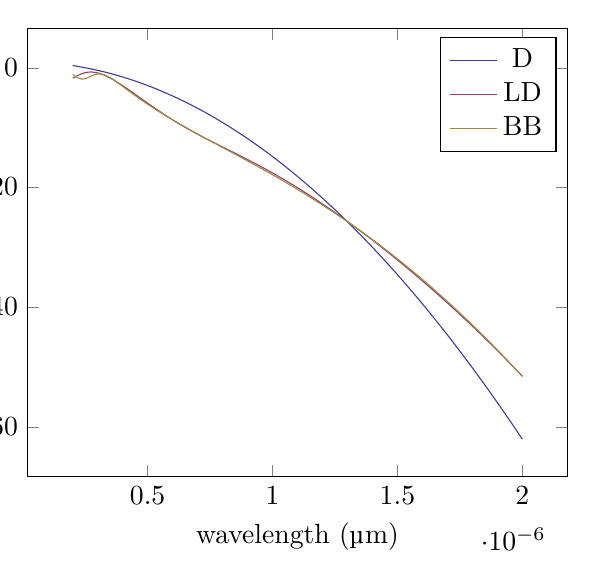
\begin{tikzpicture}[baseline,trim axis left]
\begin{axis}[xlabel=wavelength (\si{\micro\meter}),ylabel=$\epsilon'$]
\addplot[color=colora] coordinates {
(2e-07, 0.366919879819)
(2.18181818182e-07, 0.246590921646)
(2.36363636364e-07, 0.115801686173)
(2.54545454545e-07, -0.0254470491442)
(2.72727272727e-07, -0.177154444705)
(2.90909090909e-07, -0.339319598782)
(3.09090909091e-07, -0.511941547529)
(3.27272727273e-07, -0.695019264998)
(3.45454545455e-07, -0.888551663154)
(3.63636363636e-07, -1.09253759189)
(3.81818181818e-07, -1.30697583905)
(4e-07, -1.53186513044)
(4.18181818182e-07, -1.76720412984)
(4.36363636364e-07, -2.01299143905)
(4.54545454545e-07, -2.26922559787)
(4.72727272727e-07, -2.53590508418)
(4.90909090909e-07, -2.8130283139)
(5.09090909091e-07, -3.10059364105)
(5.27272727273e-07, -3.39859935776)
(5.45454545455e-07, -3.70704369431)
(5.63636363636e-07, -4.02592481915)
(5.81818181818e-07, -4.35524083891)
(6e-07, -4.69498979846)
(6.18181818182e-07, -5.04516968091)
(6.36363636364e-07, -5.40577840766)
(6.54545454545e-07, -5.77681383841)
(6.72727272727e-07, -6.15827377123)
(6.90909090909e-07, -6.55015594253)
(7.09090909091e-07, -6.95245802716)
(7.27272727273e-07, -7.3651776384)
(7.45454545455e-07, -7.78831232803)
(7.63636363636e-07, -8.22185958631)
(7.81818181818e-07, -8.66581684209)
(8e-07, -9.12018146279)
(8.18181818182e-07, -9.58495075448)
(8.36363636364e-07, -10.0601219619)
(8.54545454545e-07, -10.5456922684)
(8.72727272727e-07, -11.0416587963)
(8.90909090909e-07, -11.5480186066)
(9.09090909091e-07, -12.064768699)
(9.27272727273e-07, -12.5919060122)
(9.45454545455e-07, -13.129427424)
(9.63636363636e-07, -13.677329751)
(9.81818181818e-07, -14.2356097487)
(1e-06, -14.8042641119)
(1.01818181818e-06, -15.3832894744)
(1.03636363636e-06, -15.9726824092)
(1.05454545455e-06, -16.5724394285)
(1.07272727273e-06, -17.1825569838)
(1.09090909091e-06, -17.8030314659)
(1.10909090909e-06, -18.4338592051)
(1.12727272727e-06, -19.0750364708)
(1.14545454545e-06, -19.7265594723)
(1.16363636364e-06, -20.3884243581)
(1.18181818182e-06, -21.0606272165)
(1.2e-06, -21.7431640754)
(1.21818181818e-06, -22.4360309025)
(1.23636363636e-06, -23.139223605)
(1.25454545455e-06, -23.8527380302)
(1.27272727273e-06, -24.5765699652)
(1.29090909091e-06, -25.3107151371)
(1.30909090909e-06, -26.055169213)
(1.32727272727e-06, -26.8099278)
(1.34545454545e-06, -27.5749864455)
(1.36363636364e-06, -28.350340637)
(1.38181818182e-06, -29.1359858023)
(1.4e-06, -29.9319173096)
(1.41818181818e-06, -30.7381304675)
(1.43636363636e-06, -31.5546205249)
(1.45454545455e-06, -32.3813826717)
(1.47272727273e-06, -33.2184120378)
(1.49090909091e-06, -34.0657036944)
(1.50909090909e-06, -34.9232526531)
(1.52727272727e-06, -35.7910538665)
(1.54545454545e-06, -36.6691022279)
(1.56363636364e-06, -37.5573925719)
(1.58181818182e-06, -38.455919674)
(1.6e-06, -39.3646782508)
(1.61818181818e-06, -40.2836629602)
(1.63636363636e-06, -41.2128684014)
(1.65454545455e-06, -42.1522891149)
(1.67272727273e-06, -43.1019195827)
(1.69090909091e-06, -44.0617542284)
(1.70909090909e-06, -45.0317874171)
(1.72727272727e-06, -46.0120134556)
(1.74545454545e-06, -47.0024265927)
(1.76363636364e-06, -48.0030210188)
(1.78181818182e-06, -49.0137908663)
(1.8e-06, -50.0347302099)
(1.81818181818e-06, -51.065833066)
(1.83636363636e-06, -52.1070933936)
(1.85454545455e-06, -53.1585050937)
(1.87272727273e-06, -54.2200620099)
(1.89090909091e-06, -55.2917579281)
(1.90909090909e-06, -56.3735865769)
(1.92727272727e-06, -57.4655416276)
(1.94545454545e-06, -58.5676166941)
(1.96363636364e-06, -59.6798053332)
(1.98181818182e-06, -60.8021010447)
(2e-06, -61.9344972713)
};
\addlegendentry{D}
\addplot[color=colorb] coordinates {
(2e-07, -1.7423226919)
(2.18181818182e-07, -1.33943218694)
(2.36363636364e-07, -0.988197444975)
(2.54545454545e-07, -0.765535064291)
(2.72727272727e-07, -0.694534330282)
(2.90909090909e-07, -0.765764625643)
(3.09090909091e-07, -0.956852463288)
(3.27272727273e-07, -1.24357470509)
(3.45454545455e-07, -1.60440299926)
(3.63636363636e-07, -2.02162456209)
(3.81818181818e-07, -2.48107527988)
(4e-07, -2.97147694731)
(4.18181818182e-07, -3.48377615924)
(4.36363636364e-07, -4.01060847044)
(4.54545454545e-07, -4.54590257864)
(4.72727272727e-07, -5.08460333209)
(4.90909090909e-07, -5.62248510938)
(5.09090909091e-07, -6.15602965221)
(5.27272727273e-07, -6.68234738238)
(5.45454545455e-07, -7.19912607465)
(5.63636363636e-07, -7.70459483481)
(5.81818181818e-07, -8.19749463452)
(6e-07, -8.67704933299)
(6.18181818182e-07, -9.14293331399)
(6.36363636364e-07, -9.59523367826)
(6.54545454545e-07, -10.0344064011)
(6.72727272727e-07, -10.4612270072)
(6.90909090909e-07, -10.8767371344)
(7.09090909091e-07, -11.2821888642)
(7.27272727273e-07, -11.6789889107)
(7.45454545455e-07, -12.0686447269)
(7.63636363636e-07, -12.4527143532)
(7.81818181818e-07, -12.8327614701)
(8e-07, -13.2103166749)
(8.18181818182e-07, -13.5868455555)
(8.36363636364e-07, -13.9637237038)
(8.54545454545e-07, -14.3422184569)
(8.72727272727e-07, -14.7234768668)
(8.90909090909e-07, -15.108519206)
(9.09090909091e-07, -15.4982372003)
(9.27272727273e-07, -15.8933961363)
(9.45454545455e-07, -16.2946400031)
(9.63636363636e-07, -16.7024988844)
(9.81818181818e-07, -17.1173978977)
(1e-06, -17.5396670766)
(1.01818181818e-06, -17.9695516954)
(1.03636363636e-06, -18.407222633)
(1.05454545455e-06, -18.8527864708)
(1.07272727273e-06, -19.3062950982)
(1.09090909091e-06, -19.7677546709)
(1.10909090909e-06, -20.2371338277)
(1.12727272727e-06, -20.714371116)
(1.14545454545e-06, -21.1993816137)
(1.16363636364e-06, -21.6920627628)
(1.18181818182e-06, -22.1922994484)
(1.2e-06, -22.6999683704)
(1.21818181818e-06, -23.2149417639)
(1.23636363636e-06, -23.7370905268)
(1.25454545455e-06, -24.266286815)
(1.27272727273e-06, -24.802406166)
(1.29090909091e-06, -25.3453292047)
(1.30909090909e-06, -25.8949429879)
(1.32727272727e-06, -26.451142034)
(1.34545454545e-06, -27.013829084)
(1.36363636364e-06, -27.5829156328)
(1.38181818182e-06, -28.1583222679)
(1.4e-06, -28.7399788457)
(1.41818181818e-06, -29.3278245344)
(1.43636363636e-06, -29.9218077462)
(1.45454545455e-06, -30.5218859817)
(1.47272727273e-06, -31.1280256021)
(1.49090909091e-06, -31.7402015469)
(1.50909090909e-06, -32.3583970083)
(1.52727272727e-06, -32.9826030748)
(1.54545454545e-06, -33.6128183516)
(1.56363636364e-06, -34.2490485683)
(1.58181818182e-06, -34.8913061767)
(1.6e-06, -35.5396099479)
(1.61818181818e-06, -36.1939845689)
(1.63636363636e-06, -36.8544602464)
(1.65454545455e-06, -37.5210723174)
(1.67272727273e-06, -38.1938608696)
(1.69090909091e-06, -38.8728703742)
(1.70909090909e-06, -39.5581493316)
(1.72727272727e-06, -40.2497499305)
(1.74545454545e-06, -40.9477277215)
(1.76363636364e-06, -41.652141306)
(1.78181818182e-06, -42.3630520392)
(1.8e-06, -43.0805237486)
(1.81818181818e-06, -43.804622467)
(1.83636363636e-06, -44.5354161797)
(1.85454545455e-06, -45.2729745865)
(1.87272727273e-06, -46.0173688769)
(1.89090909091e-06, -46.7686715185)
(1.90909090909e-06, -47.526956059)
(1.92727272727e-06, -48.2922969395)
(1.94545454545e-06, -49.0647693203)
(1.96363636364e-06, -49.8444489179)
(1.98181818182e-06, -50.6314118525)
(2e-06, -51.4257345057)
};
\addlegendentry{LD}
\addplot[color=colorc] coordinates {
(2e-07, -1.13506304201)
(2.18181818182e-07, -1.61339600083)
(2.36363636364e-07, -1.88644346466)
(2.54545454545e-07, -1.77532890809)
(2.72727272727e-07, -1.41321209785)
(2.90909090909e-07, -1.09555289816)
(3.09090909091e-07, -1.0101894288)
(3.27272727273e-07, -1.17789919418)
(3.45454545455e-07, -1.53484852176)
(3.63636363636e-07, -2.00701860122)
(3.81818181818e-07, -2.53897579558)
(4e-07, -3.09600169554)
(4.18181818182e-07, -3.65832804084)
(4.36363636364e-07, -4.21539561386)
(4.54545454545e-07, -4.76192397888)
(4.72727272727e-07, -5.29556052631)
(4.90909090909e-07, -5.81555335874)
(5.09090909091e-07, -6.32201892129)
(5.27272727273e-07, -6.81553920937)
(5.45454545455e-07, -7.29693891746)
(5.63636363636e-07, -7.76716069554)
(5.81818181818e-07, -8.22719441633)
(6e-07, -8.67803661002)
(6.18181818182e-07, -9.12066705428)
(6.36363636364e-07, -9.55603531875)
(6.54545454545e-07, -9.98505320995)
(6.72727272727e-07, -10.4085907902)
(6.90909090909e-07, -10.8274746064)
(7.09090909091e-07, -11.2424873105)
(7.27272727273e-07, -11.6543681677)
(7.45454545455e-07, -12.0638141349)
(7.63636363636e-07, -12.471481302)
(7.81818181818e-07, -12.8779865602)
(8e-07, -13.2839094009)
(8.18181818182e-07, -13.6897937823)
(8.36363636364e-07, -14.0961500157)
(8.54545454545e-07, -14.5034566392)
(8.72727272727e-07, -14.9121622554)
(8.90909090909e-07, -15.322687315)
(9.09090909091e-07, -15.7354258372)
(9.27272727273e-07, -16.1507470565)
(9.45454545455e-07, -16.5689969929)
(9.63636363636e-07, -16.9904999419)
(9.81818181818e-07, -17.4155598847)
(1e-06, -17.8444618172)
(1.01818181818e-06, -18.2774730015)
(1.03636363636e-06, -18.71484414)
(1.05454545455e-06, -19.1568104764)
(1.07272727273e-06, -19.6035928258)
(1.09090909091e-06, -20.0553985376)
(1.10909090909e-06, -20.5124223941)
(1.12727272727e-06, -20.974847449)
(1.14545454545e-06, -21.4428458089)
(1.16363636364e-06, -21.9165793615)
(1.18181818182e-06, -22.3962004529)
(1.2e-06, -22.8818525188)
(1.21818181818e-06, -23.3736706711)
(1.23636363636e-06, -23.8717822441)
(1.25454545455e-06, -24.3763073021)
(1.27272727273e-06, -24.8873591116)
(1.29090909091e-06, -25.4050445811)
(1.30909090909e-06, -25.9294646688)
(1.32727272727e-06, -26.4607147631)
(1.34545454545e-06, -26.9988850362)
(1.36363636364e-06, -27.5440607729)
(1.38181818182e-06, -28.0963226765)
(1.4e-06, -28.6557471542)
(1.41818181818e-06, -29.2224065824)
(1.43636363636e-06, -29.7963695535)
(1.45454545455e-06, -30.3777011069)
(1.47272727273e-06, -30.9664629428)
(1.49090909091e-06, -31.5627136229)
(1.50909090909e-06, -32.1665087571)
(1.52727272727e-06, -32.7779011772)
(1.54545454545e-06, -33.3969411)
(1.56363636364e-06, -34.0236762787)
(1.58181818182e-06, -34.6581521452)
(1.6e-06, -35.300413383)
(1.61818181818e-06, -35.950498294)
(1.63636363636e-06, -36.6084475407)
(1.65454545455e-06, -37.2742985107)
(1.67272727273e-06, -37.9480868527)
(1.69090909091e-06, -38.6298465711)
(1.70909090909e-06, -39.3196101158)
(1.72727272727e-06, -40.0174084653)
(1.74545454545e-06, -40.7232712051)
(1.76363636364e-06, -41.4372266019)
(1.78181818182e-06, -42.1593016716)
(1.8e-06, -42.8895222451)
(1.81818181818e-06, -43.6279130286)
(1.83636363636e-06, -44.3744976614)
(1.85454545455e-06, -45.1292987694)
(1.87272727273e-06, -45.8923380158)
(1.89090909091e-06, -46.6636361492)
(1.90909090909e-06, -47.4432130479)
(1.92727272727e-06, -48.2310877629)
(1.94545454545e-06, -49.0272785576)
(1.96363636364e-06, -49.8318029451)
(1.98181818182e-06, -50.6446777242)
(2e-06, -51.4659190126)
};
\addlegendentry{BB}
\end{axis}
\end{tikzpicture}%
\\
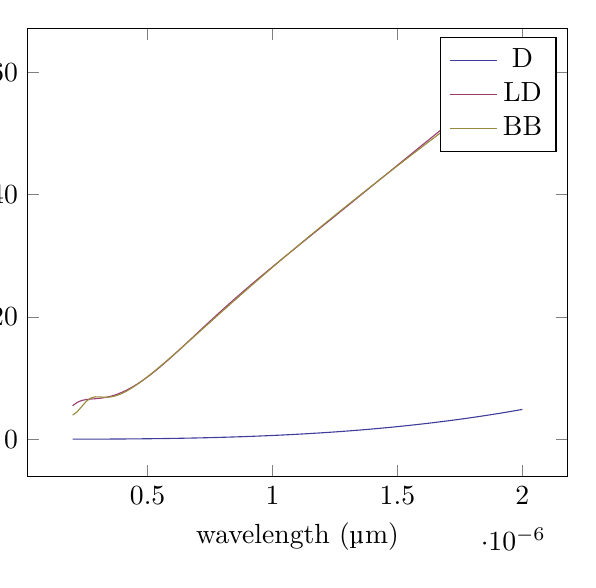
\begin{tikzpicture}[baseline,trim axis left]
\begin{axis}[xlabel=wavelength (\si{\micro\meter}),ylabel=$\epsilon''$]
\addplot[color=colora] coordinates {
(2e-07, 0.00490189032214)
(2.18181818182e-07, 0.00636391431566)
(2.36363636364e-07, 0.00809105704722)
(2.54545454545e-07, 0.0101053998871)
(2.72727272727e-07, 0.0124290213604)
(2.90909090909e-07, 0.0150839969287)
(3.09090909091e-07, 0.018092398771)
(3.27272727273e-07, 0.0214762955659)
(3.45454545455e-07, 0.025257752273)
(3.63636363636e-07, 0.0294588299144)
(3.81818181818e-07, 0.0341015853568)
(4e-07, 0.0392080710932)
(4.18181818182e-07, 0.044800335025)
(4.36363636364e-07, 0.050900420244)
(4.54545454545e-07, 0.0575303648144)
(4.72727272727e-07, 0.0647122015554)
(4.90909090909e-07, 0.0724679578234)
(5.09090909091e-07, 0.0808196552944)
(5.27272727273e-07, 0.0897893097469)
(5.45454545455e-07, 0.0993989308441)
(5.63636363636e-07, 0.109670521918)
(5.81818181818e-07, 0.120626079749)
(6e-07, 0.132287594356)
(6.18181818182e-07, 0.144677048771)
(6.36363636364e-07, 0.157816418828)
(6.54545454545e-07, 0.171727672947)
(6.72727272727e-07, 0.186432771913)
(6.90909090909e-07, 0.201953668665)
(7.09090909091e-07, 0.218312308078)
(7.27272727273e-07, 0.235530626745)
(7.45454545455e-07, 0.253630552767)
(7.63636363636e-07, 0.27263400553)
(7.81818181818e-07, 0.292562895497)
(8e-07, 0.313439123987)
(8.18181818182e-07, 0.335284582966)
(8.36363636364e-07, 0.358121154827)
(8.54545454545e-07, 0.381970712177)
(8.72727272727e-07, 0.406855117625)
(8.90909090909e-07, 0.432796223565)
(9.09090909091e-07, 0.459815871964)
(9.27272727273e-07, 0.487935894148)
(9.45454545455e-07, 0.517178110588)
(9.63636363636e-07, 0.547564330685)
(9.81818181818e-07, 0.579116352562)
(1e-06, 0.611855962847)
(1.01818181818e-06, 0.645804936462)
(1.03636363636e-06, 0.68098503641)
(1.05454545455e-06, 0.717418013564)
(1.07272727273e-06, 0.755125606453)
(1.09090909091e-06, 0.794129541055)
(1.10909090909e-06, 0.834451530581)
(1.12727272727e-06, 0.876113275266)
(1.14545454545e-06, 0.919136462158)
(1.16363636364e-06, 0.963542764909)
(1.18181818182e-06, 1.00935384356)
(1.2e-06, 1.05659134434)
(1.21818181818e-06, 1.10527689945)
(1.23636363636e-06, 1.15543212685)
(1.25454545455e-06, 1.20707863005)
(1.27272727273e-06, 1.26023799793)
(1.29090909091e-06, 1.31493180447)
(1.30909090909e-06, 1.37118160861)
(1.32727272727e-06, 1.42900895401)
(1.34545454545e-06, 1.48843536882)
(1.36363636364e-06, 1.54948236552)
(1.38181818182e-06, 1.61217144068)
(1.4e-06, 1.67652407476)
(1.41818181818e-06, 1.74256173192)
(1.43636363636e-06, 1.81030585979)
(1.45454545455e-06, 1.87977788928)
(1.47272727273e-06, 1.95099923436)
(1.49090909091e-06, 2.02399129189)
(1.50909090909e-06, 2.09877544137)
(1.52727272727e-06, 2.17537304475)
(1.54545454545e-06, 2.25380544627)
(1.56363636364e-06, 2.33409397218)
(1.58181818182e-06, 2.41625993059)
(1.6e-06, 2.50032461127)
(1.61818181818e-06, 2.58630928541)
(1.63636363636e-06, 2.67423520545)
(1.65454545455e-06, 2.76412360486)
(1.67272727273e-06, 2.85599569796)
(1.69090909091e-06, 2.9498726797)
(1.70909090909e-06, 3.04577572547)
(1.72727272727e-06, 3.14372599088)
(1.74545454545e-06, 3.2437446116)
(1.76363636364e-06, 3.34585270311)
(1.78181818182e-06, 3.45007136056)
(1.8e-06, 3.55642165851)
(1.81818181818e-06, 3.66492465078)
(1.83636363636e-06, 3.77560137024)
(1.85454545455e-06, 3.88847282858)
(1.87272727273e-06, 4.00356001617)
(1.89090909091e-06, 4.12088390183)
(1.90909090909e-06, 4.24046543262)
(1.92727272727e-06, 4.36232553368)
(1.94545454545e-06, 4.48648510802)
(1.96363636364e-06, 4.61296503631)
(1.98181818182e-06, 4.74178617672)
(2e-06, 4.87296936468)
};
\addlegendentry{D}
\addplot[color=colorb] coordinates {
(2e-07, 5.48316698957)
(2.18181818182e-07, 6.02648980647)
(2.36363636364e-07, 6.33993538287)
(2.54545454545e-07, 6.49596066433)
(2.72727272727e-07, 6.5716107484)
(2.90909090909e-07, 6.62559769294)
(3.09090909091e-07, 6.69528019472)
(3.27272727273e-07, 6.8016224314)
(3.45454545455e-07, 6.95500481134)
(3.63636363636e-07, 7.15957634164)
(3.81818181818e-07, 7.41601176013)
(4e-07, 7.7231128691)
(4.18181818182e-07, 8.07868886294)
(4.36363636364e-07, 8.48001992133)
(4.54545454545e-07, 8.92409189739)
(4.72727272727e-07, 9.40771141334)
(4.90909090909e-07, 9.92756293208)
(5.09090909091e-07, 10.4802415867)
(5.27272727273e-07, 11.0622796158)
(5.45454545455e-07, 11.6701750934)
(5.63636363636e-07, 12.3004263155)
(5.81818181818e-07, 12.9495720835)
(6e-07, 13.6142363221)
(6.18181818182e-07, 14.2911745216)
(6.36363636364e-07, 14.9773191281)
(6.54545454545e-07, 15.6698210802)
(6.72727272727e-07, 16.3660850651)
(6.90909090909e-07, 17.0637966634)
(7.09090909091e-07, 17.7609402554)
(7.27272727273e-07, 18.4558072869)
(7.45454545455e-07, 19.1469951756)
(7.63636363636e-07, 19.8333976991)
(7.81818181818e-07, 20.5141881312)
(8e-07, 21.1887966484)
(8.18181818182e-07, 21.8568836387)
(8.36363636364e-07, 22.5183105123)
(8.54545454545e-07, 23.1731094832)
(8.72727272727e-07, 23.8214535881)
(8.90909090909e-07, 24.4636279623)
(9.09090909091e-07, 25.1000031426)
(9.27272727273e-07, 25.7310109193)
(9.45454545455e-07, 26.357123043)
(9.63636363636e-07, 26.9788329064)
(9.81818181818e-07, 27.5966401736)
(1e-06, 28.211038219)
(1.01818181818e-06, 28.8225041635)
(1.03636363636e-06, 29.4314912461)
(1.05454545455e-06, 30.0384232472)
(1.07272727273e-06, 30.643690676)
(1.09090909091e-06, 31.2476484414)
(1.10909090909e-06, 31.8506147462)
(1.12727272727e-06, 32.4528709665)
(1.14545454545e-06, 33.0546623057)
(1.16363636364e-06, 33.6561990396)
(1.18181818182e-06, 34.2576581981)
(1.2e-06, 34.8591855506)
(1.21818181818e-06, 35.4608977882)
(1.23636363636e-06, 36.0628848163)
(1.25454545455e-06, 36.6652120866)
(1.27272727273e-06, 37.2679229159)
(1.29090909091e-06, 37.8710407503)
(1.30909090909e-06, 38.474571344)
(1.32727272727e-06, 39.0785048326)
(1.34545454545e-06, 39.6828176857)
(1.36363636364e-06, 40.2874745309)
(1.38181818182e-06, 40.8924298446)
(1.4e-06, 41.4976295105)
(1.41818181818e-06, 42.1030122466)
(1.43636363636e-06, 42.708510905)
(1.45454545455e-06, 43.3140536506)
(1.47272727273e-06, 43.919565025)
(1.49090909091e-06, 44.5249669009)
(1.50909090909e-06, 45.1301793371)
(1.52727272727e-06, 45.7351213387)
(1.54545454545e-06, 46.339711531)
(1.56363636364e-06, 46.9438687543)
(1.58181818182e-06, 47.5475125853)
(1.6e-06, 48.1505637931)
(1.61818181818e-06, 48.7529447337)
(1.63636363636e-06, 49.3545796912)
(1.65454545455e-06, 49.9553951684)
(1.67272727273e-06, 50.5553201337)
(1.69090909091e-06, 51.1542862279)
(1.70909090909e-06, 51.7522279347)
(1.72727272727e-06, 52.3490827197)
(1.74545454545e-06, 52.9447911404)
(1.76363636364e-06, 53.5392969309)
(1.78181818182e-06, 54.1325470638)
(1.8e-06, 54.724491792)
(1.81818181818e-06, 55.3150846736)
(1.83636363636e-06, 55.9042825799)
(1.85454545455e-06, 56.4920456911)
(1.87272727273e-06, 57.0783374788)
(1.89090909091e-06, 57.6631246795)
(1.90909090909e-06, 58.2463772576)
(1.92727272727e-06, 58.8280683623)
(1.94545454545e-06, 59.408174276)
(1.96363636364e-06, 59.986674359)
(1.98181818182e-06, 60.5635509879)
(2e-06, 61.138789491)
};
\addlegendentry{LD}
\addplot[color=colorc] coordinates {
(2e-07, 3.94363470032)
(2.18181818182e-07, 4.49905940592)
(2.36363636364e-07, 5.34188580327)
(2.54545454545e-07, 6.19531953536)
(2.72727272727e-07, 6.74933458025)
(2.90909090909e-07, 6.94198554902)
(3.09090909091e-07, 6.9235042118)
(3.27272727273e-07, 6.86877071687)
(3.45454545455e-07, 6.88204895218)
(3.63636363636e-07, 7.00000469987)
(3.81818181818e-07, 7.22233615762)
(4e-07, 7.5348865502)
(4.18181818182e-07, 7.92106070071)
(4.36363636364e-07, 8.36604413665)
(4.54545454545e-07, 8.85777322946)
(4.72727272727e-07, 9.38673794542)
(4.90909090909e-07, 9.94549179504)
(5.09090909091e-07, 10.5281749069)
(5.27272727273e-07, 11.130129848)
(5.45454545455e-07, 11.7476123784)
(5.63636363636e-07, 12.377578784)
(5.81818181818e-07, 13.0175300448)
(6e-07, 13.6653968521)
(6.18181818182e-07, 14.3194537086)
(6.36363636364e-07, 14.97825379)
(6.54545454545e-07, 15.6405787632)
(6.72727272727e-07, 16.3053995173)
(6.90909090909e-07, 16.9718449803)
(7.09090909091e-07, 17.6391770173)
(7.27272727273e-07, 18.3067699815)
(7.45454545455e-07, 18.9740938756)
(7.63636363636e-07, 19.6407003598)
(7.81818181818e-07, 20.3062110324)
(8e-07, 20.9703075485)
(8.18181818182e-07, 21.6327232401)
(8.36363636364e-07, 22.2932359776)
(8.54545454545e-07, 22.9516620616)
(8.72727272727e-07, 23.6078509812)
(8.90909090909e-07, 24.2616809018)
(9.09090909091e-07, 24.9130547718)
(9.27272727273e-07, 25.5618969567)
(9.45454545455e-07, 26.2081503251)
(9.63636363636e-07, 26.8517737211)
(9.81818181818e-07, 27.4927397698)
(1e-06, 28.1310329711)
(1.01818181818e-06, 28.766648041)
(1.03636363636e-06, 29.3995884688)
(1.05454545455e-06, 30.0298652606)
(1.07272727273e-06, 30.6574958451)
(1.09090909091e-06, 31.2825031203)
(1.10909090909e-06, 31.904914623)
(1.12727272727e-06, 32.5247618056)
(1.14545454545e-06, 33.1420794053)
(1.16363636364e-06, 33.7569048961)
(1.18181818182e-06, 34.3692780102)
(1.2e-06, 34.9792403233)
(1.21818181818e-06, 35.5868348927)
(1.23636363636e-06, 36.1921059439)
(1.25454545455e-06, 36.7950985982)
(1.27272727273e-06, 37.3958586372)
(1.29090909091e-06, 37.9944322985)
(1.30909090909e-06, 38.5908660997)
(1.32727272727e-06, 39.1852066869)
(1.34545454545e-06, 39.7775007039)
(1.36363636364e-06, 40.3677946811)
(1.38181818182e-06, 40.9561349399)
(1.4e-06, 41.5425675119)
(1.41818181818e-06, 42.1271380704)
(1.43636363636e-06, 42.7098918733)
(1.45454545455e-06, 43.2908737148)
(1.47272727273e-06, 43.8701278862)
(1.49090909091e-06, 44.4476981436)
(1.50909090909e-06, 45.0236276823)
(1.52727272727e-06, 45.5979591162)
(1.54545454545e-06, 46.1707344627)
(1.56363636364e-06, 46.7419951311)
(1.58181818182e-06, 47.3117819151)
(1.6e-06, 47.8801348936)
(1.61818181818e-06, 48.4470937838)
(1.63636363636e-06, 49.0126974445)
(1.65454545455e-06, 49.5769841875)
(1.67272727273e-06, 50.1399917096)
(1.69090909091e-06, 50.7017570987)
(1.70909090909e-06, 51.2623168406)
(1.72727272727e-06, 51.8217068266)
(1.74545454545e-06, 52.3799623626)
(1.76363636364e-06, 52.9371181785)
(1.78181818182e-06, 53.493208438)
(1.8e-06, 54.0482667489)
(1.81818181818e-06, 54.6023261745)
(1.83636363636e-06, 55.1554192439)
(1.85454545455e-06, 55.7075779638)
(1.87272727273e-06, 56.2588338294)
(1.89090909091e-06, 56.8092178364)
(1.90909090909e-06, 57.3587604916)
(1.92727272727e-06, 57.9074918252)
(1.94545454545e-06, 58.4554414012)
(1.96363636364e-06, 59.0026383294)
(1.98181818182e-06, 59.549111276)
(2e-06, 60.0948884749)
};
\addlegendentry{BB}
\end{axis}
\end{tikzpicture}%
\\
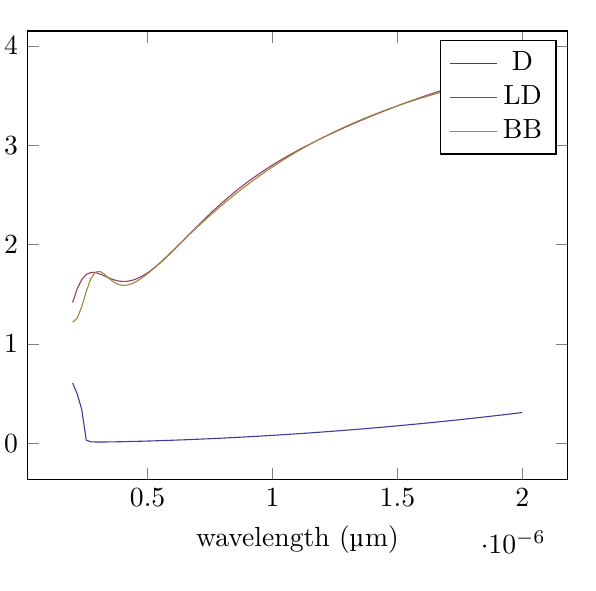
\begin{tikzpicture}[baseline,trim axis left]
\begin{axis}[xlabel=wavelength (\si{\micro\meter}),ylabel=$n'$]
\addplot[color=colora] coordinates {
(2e-07, 0.605752631749)
(2.18181818182e-07, 0.496620553455)
(2.36363636364e-07, 0.340503809856)
(2.54545454545e-07, 0.0310892183638)
(2.72727272727e-07, 0.014755848483)
(2.90909090909e-07, 0.012944186719)
(3.09090909091e-07, 0.0126411969141)
(3.27272727273e-07, 0.0128789109167)
(3.45454545455e-07, 0.0133961348282)
(3.63636363636e-07, 0.0140905467387)
(3.81818181818e-07, 0.0149133031357)
(4e-07, 0.0158379752995)
(4.18181818182e-07, 0.0168489571967)
(4.36363636364e-07, 0.017936417603)
(4.54545454545e-07, 0.0190938458111)
(4.72727272727e-07, 0.0203167548345)
(4.90909090909e-07, 0.0216019500048)
(5.09090909091e-07, 0.0229470941472)
(5.27272727273e-07, 0.0243504375851)
(5.45454545455e-07, 0.0258106442572)
(5.63636363636e-07, 0.0273266761886)
(5.81818181818e-07, 0.0288977146414)
(6e-07, 0.0305231050223)
(6.18181818182e-07, 0.0322023175863)
(6.36363636364e-07, 0.0339349188892)
(6.54545454545e-07, 0.0357205507066)
(6.72727272727e-07, 0.0375589142363)
(6.90909090909e-07, 0.0394497581006)
(7.09090909091e-07, 0.041392869125)
(7.27272727273e-07, 0.0433880651711)
(7.45454545455e-07, 0.0454351895104)
(7.63636363636e-07, 0.0475341063659)
(7.81818181818e-07, 0.049684697349)
(8e-07, 0.0518868585896)
(8.18181818182e-07, 0.0541404984062)
(8.36363636364e-07, 0.0564455354032)
(8.54545454545e-07, 0.0588018969055)
(8.72727272727e-07, 0.0612095176632)
(8.90909090909e-07, 0.0636683387748)
(9.09090909091e-07, 0.0661783067862)
(9.27272727273e-07, 0.0687393729329)
(9.45454545455e-07, 0.0713514925009)
(9.63636363636e-07, 0.0740146242839)
(9.81818181818e-07, 0.0767287301215)
(1e-06, 0.079493774504)
(1.01818181818e-06, 0.0823097242328)
(1.03636363636e-06, 0.0851765481288)
(1.05454545455e-06, 0.0880942167793)
(1.07272727273e-06, 0.0910627023193)
(1.09090909091e-06, 0.0940819782406)
(1.10909090909e-06, 0.097152019226)
(1.12727272727e-06, 0.100272801003)
(1.14545454545e-06, 0.103444300218)
(1.16363636364e-06, 0.106666494321)
(1.18181818182e-06, 0.109939361469)
(1.2e-06, 0.113262880439)
(1.21818181818e-06, 0.116637030548)
(1.23636363636e-06, 0.120061791587)
(1.25454545455e-06, 0.123537143757)
(1.27272727273e-06, 0.127063067616)
(1.29090909091e-06, 0.13063954403)
(1.30909090909e-06, 0.134266554132)
(1.32727272727e-06, 0.137944079276)
(1.34545454545e-06, 0.141672101009)
(1.36363636364e-06, 0.145450601037)
(1.38181818182e-06, 0.149279561194)
(1.4e-06, 0.15315896342)
(1.41818181818e-06, 0.157088789736)
(1.43636363636e-06, 0.161069022224)
(1.45454545455e-06, 0.165099643005)
(1.47272727273e-06, 0.169180634226)
(1.49090909091e-06, 0.173311978043)
(1.50909090909e-06, 0.177493656603)
(1.52727272727e-06, 0.181725652036)
(1.54545454545e-06, 0.186007946441)
(1.56363636364e-06, 0.190340521875)
(1.58181818182e-06, 0.194723360343)
(1.6e-06, 0.199156443791)
(1.61818181818e-06, 0.203639754094)
(1.63636363636e-06, 0.208173273052)
(1.65454545455e-06, 0.21275698238)
(1.67272727273e-06, 0.217390863706)
(1.69090909091e-06, 0.222074898558)
(1.70909090909e-06, 0.226809068366)
(1.72727272727e-06, 0.231593354454)
(1.74545454545e-06, 0.236427738033)
(1.76363636364e-06, 0.241312200201)
(1.78181818182e-06, 0.246246721937)
(1.8e-06, 0.251231284098)
(1.81818181818e-06, 0.256265867414)
(1.83636363636e-06, 0.261350452487)
(1.85454545455e-06, 0.266485019787)
(1.87272727273e-06, 0.271669549652)
(1.89090909091e-06, 0.27690402228)
(1.90909090909e-06, 0.282188417734)
(1.92727272727e-06, 0.287522715933)
(1.94545454545e-06, 0.292906896656)
(1.96363636364e-06, 0.298340939535)
(1.98181818182e-06, 0.303824824058)
(2e-06, 0.309358529565)
};
\addlegendentry{D}
\addplot[color=colorb] coordinates {
(2e-07, 1.41615809961)
(2.18181818182e-07, 1.55468852531)
(2.36363636364e-07, 1.64746628034)
(2.54545454545e-07, 1.69932021635)
(2.72727272727e-07, 1.71954589223)
(2.90909090909e-07, 1.71812958402)
(3.09090909091e-07, 1.70388616978)
(3.27272727273e-07, 1.68386426105)
(3.45454545455e-07, 1.66331863239)
(3.63636363636e-07, 1.64588854763)
(3.81818181818e-07, 1.63385446774)
(4e-07, 1.62842786637)
(4.18181818182e-07, 1.63003978082)
(4.36363636364e-07, 1.63859617113)
(4.54545454545e-07, 1.65368046493)
(4.72727272727e-07, 1.67469955344)
(4.90909090909e-07, 1.70098075583)
(5.09090909091e-07, 1.73183175633)
(5.27272727273e-07, 1.76657522456)
(5.45454545455e-07, 1.80456741699)
(5.63636363636e-07, 1.84520729598)
(5.81818181818e-07, 1.88794038583)
(6e-07, 1.93225990136)
(6.18181818182e-07, 1.97770656453)
(6.36363636364e-07, 2.02386782668)
(6.54545454545e-07, 2.07037680557)
(6.72727272727e-07, 2.11691102666)
(6.90909090909e-07, 2.16319095537)
(7.09090909091e-07, 2.20897827456)
(7.27272727273e-07, 2.2540738671)
(7.45454545455e-07, 2.29831548796)
(7.63636363636e-07, 2.34157513972)
(7.81818181818e-07, 2.38375619335)
(8e-07, 2.42479031684)
(8.18181818182e-07, 2.46463428757)
(8.36363636364e-07, 2.50326676911)
(8.54545454545e-07, 2.54068513085)
(8.72727272727e-07, 2.57690238122)
(8.90909090909e-07, 2.61194427363)
(9.09090909091e-07, 2.64584663117)
(9.27272727273e-07, 2.67865292172)
(9.45454545455e-07, 2.71041210211)
(9.63636363636e-07, 2.74117673796)
(9.81818181818e-07, 2.77100139575)
(1e-06, 2.79994129577)
(1.01818181818e-06, 2.82805120874)
(1.03636363636e-06, 2.85538457488)
(1.05454545455e-06, 2.88199282198)
(1.07272727273e-06, 2.90792485823)
(1.09090909091e-06, 2.93322671541)
(1.10909090909e-06, 2.95794131959)
(1.12727272727e-06, 2.98210836759)
(1.14545454545e-06, 3.00576428974)
(1.16363636364e-06, 3.02894228129)
(1.18181818182e-06, 3.0516723873)
(1.2e-06, 3.07398162775)
(1.21818181818e-06, 3.09589415167)
(1.23636363636e-06, 3.11743141102)
(1.25454545455e-06, 3.13861234662)
(1.27272727273e-06, 3.15945357993)
(1.29090909091e-06, 3.17996960586)
(1.30909090909e-06, 3.20017298275)
(1.32727272727e-06, 3.22007451658)
(1.34545454545e-06, 3.23968343757)
(1.36363636364e-06, 3.25900756737)
(1.38181818182e-06, 3.27805347622)
(1.4e-06, 3.29682662937)
(1.41818181818e-06, 3.31533152258)
(1.43636363636e-06, 3.33357180685)
(1.45454545455e-06, 3.35155040253)
(1.47272727273e-06, 3.36926960325)
(1.49090909091e-06, 3.38673117008)
(1.50909090909e-06, 3.40393641654)
(1.52727272727e-06, 3.42088628497)
(1.54545454545e-06, 3.43758141499)
(1.56363636364e-06, 3.45402220441)
(1.58181818182e-06, 3.47020886342)
(1.6e-06, 3.48614146255)
(1.61818181818e-06, 3.5018199748)
(1.63636363636e-06, 3.51724431279)
(1.65454545455e-06, 3.53241436099)
(1.67272727273e-06, 3.54733000387)
(1.69090909091e-06, 3.56199115013)
(1.70909090909e-06, 3.57639775352)
(1.72727272727e-06, 3.59054983058)
(1.74545454545e-06, 3.60444747563)
(1.76363636364e-06, 3.61809087323)
(1.78181818182e-06, 3.63148030853)
(1.8e-06, 3.64461617562)
(1.81818181818e-06, 3.65749898419)
(1.83636363636e-06, 3.6701293646)
(1.85454545455e-06, 3.68250807167)
(1.87272727273e-06, 3.69463598724)
(1.89090909091e-06, 3.70651412171)
(1.90909090909e-06, 3.71814361465)
(1.92727272727e-06, 3.72952573462)
(1.94545454545e-06, 3.74066187834)
(1.96363636364e-06, 3.75155356918)
(1.98181818182e-06, 3.76220245523)
(2e-06, 3.77261030682)
};
\addlegendentry{LD}
\addplot[color=colorc] coordinates {
(2e-07, 1.2183328243)
(2.18181818182e-07, 1.25821393855)
(2.36363636364e-07, 1.37454531339)
(2.54545454545e-07, 1.52796294395)
(2.72727272727e-07, 1.6556703213)
(2.90909090909e-07, 1.72225848864)
(3.09090909091e-07, 1.7301190204)
(3.27272727273e-07, 1.70163692369)
(3.45454545455e-07, 1.66076428983)
(3.63636363636e-07, 1.6240423472)
(3.81818181818e-07, 1.59947577597)
(4e-07, 1.58904801685)
(4.18181818182e-07, 1.59165415895)
(4.36363636364e-07, 1.60509325616)
(4.54545454545e-07, 1.62707082336)
(4.72727272727e-07, 1.65558255575)
(4.90909090909e-07, 1.68900085987)
(5.09090909091e-07, 1.72604595329)
(5.27272727273e-07, 1.76572459463)
(5.45454545455e-07, 1.80726862197)
(5.63636363636e-07, 1.85008323707)
(5.81818181818e-07, 1.89370637448)
(6e-07, 1.93777769973)
(6.18181818182e-07, 1.98201521419)
(6.36363636364e-07, 2.0261976294)
(6.54545454545e-07, 2.07015104305)
(6.72727272727e-07, 2.11373880524)
(6.90909090909e-07, 2.15685375324)
(7.09090909091e-07, 2.19941221315)
(7.27272727273e-07, 2.24134932847)
(7.45454545455e-07, 2.28261539308)
(7.63636363636e-07, 2.32317295075)
(7.81818181818e-07, 2.36299448464)
(8e-07, 2.40206056475)
(8.18181818182e-07, 2.44035835349)
(8.36363636364e-07, 2.47788039374)
(8.54545454545e-07, 2.51462362101)
(8.72727272727e-07, 2.55058855489)
(8.90909090909e-07, 2.58577863464)
(9.09090909091e-07, 2.62019967136)
(9.27272727273e-07, 2.65385939506)
(9.45454545455e-07, 2.68676707919)
(9.63636363636e-07, 2.71893322883)
(9.81818181818e-07, 2.75036932129)
(1e-06, 2.78108759012)
(1.01818181818e-06, 2.81110084506)
(1.03636363636e-06, 2.84042232201)
(1.05454545455e-06, 2.869065558)
(1.07272727273e-06, 2.89704428699)
(1.09090909091e-06, 2.92437235335)
(1.10909090909e-06, 2.95106363988)
(1.12727272727e-06, 2.97713200839)
(1.14545454545e-06, 3.00259125053)
(1.16363636364e-06, 3.02745504755)
(1.18181818182e-06, 3.05173693735)
(1.2e-06, 3.07545028783)
(1.21818181818e-06, 3.09860827555)
(1.23636363636e-06, 3.12122386873)
(1.25454545455e-06, 3.14330981413)
(1.27272727273e-06, 3.164878627)
(1.29090909091e-06, 3.18594258373)
(1.30909090909e-06, 3.20651371672)
(1.32727272727e-06, 3.22660381116)
(1.34545454545e-06, 3.24622440332)
(1.36363636364e-06, 3.26538678021)
(1.38181818182e-06, 3.2841019803)
(1.4e-06, 3.30238079513)
(1.41818181818e-06, 3.32023377169)
(1.43636363636e-06, 3.33767121536)
(1.45454545455e-06, 3.35470319335)
(1.47272727273e-06, 3.37133953857)
(1.49090909091e-06, 3.38758985373)
(1.50909090909e-06, 3.40346351574)
(1.52727272727e-06, 3.41896968024)
(1.54545454545e-06, 3.43411728627)
(1.56363636364e-06, 3.448915061)
(1.58181818182e-06, 3.46337152457)
(1.6e-06, 3.47749494722)
(1.61818181818e-06, 3.49129354346)
(1.63636363636e-06, 3.50477519449)
(1.65454545455e-06, 3.51794764004)
(1.67272727273e-06, 3.53081843652)
(1.69090909091e-06, 3.54339496159)
(1.70909090909e-06, 3.55568441868)
(1.72727272727e-06, 3.56769384137)
(1.74545454545e-06, 3.57943009775)
(1.76363636364e-06, 3.5908998946)
(1.78181818182e-06, 3.60210978153)
(1.8e-06, 3.61306615503)
(1.81818181818e-06, 3.62377526233)
(1.83636363636e-06, 3.63424320524)
(1.85454545455e-06, 3.64447594387)
(1.87272727273e-06, 3.65447930025)
(1.89090909091e-06, 3.66425896178)
(1.90909090909e-06, 3.67382048473)
(1.92727272727e-06, 3.68316929747)
(1.94545454545e-06, 3.69231070376)
(1.96363636364e-06, 3.70124988583)
(1.98181818182e-06, 3.70999190742)
(2e-06, 3.71854171678)
};
\addlegendentry{BB}
\end{axis}
\end{tikzpicture}%
\\
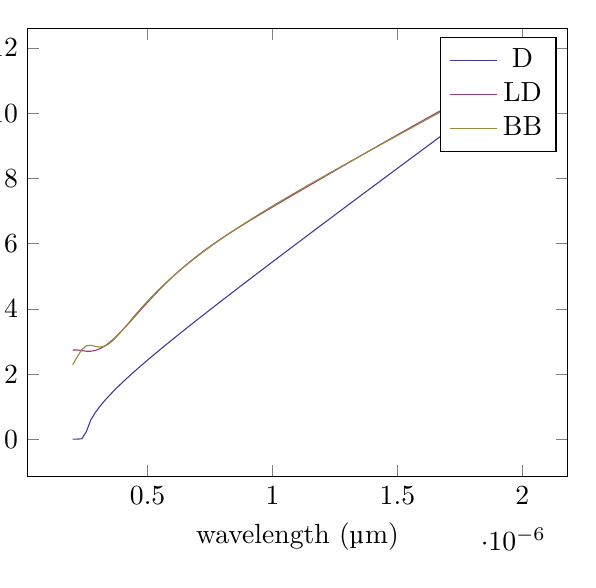
\begin{tikzpicture}[baseline,trim axis left]
\begin{axis}[xlabel=wavelength (\si{\micro\meter}),ylabel=$n''$]
\addplot[color=colora] coordinates {
(2e-07, 0.00572207152846)
(2.18181818182e-07, 0.00906117746474)
(2.36363636364e-07, 0.0168022827923)
(2.54545454545e-07, 0.22984163523)
(2.72727272727e-07, 0.595604197047)
(2.90909090909e-07, 0.823998969359)
(3.09090909091e-07, 1.01202899898)
(3.27272727273e-07, 1.17913962816)
(3.45454545455e-07, 1.3332150011)
(3.63636363636e-07, 1.47833428926)
(3.81818181818e-07, 1.61690954952)
(4e-07, 1.75049477114)
(4.18181818182e-07, 1.8801531944)
(4.36363636364e-07, 2.00664553627)
(4.54545454545e-07, 2.13053522516)
(4.72727272727e-07, 2.25225125362)
(4.90909090909e-07, 2.37212771922)
(5.09090909091e-07, 2.4904297662)
(5.27272727273e-07, 2.60737120547)
(5.45454545455e-07, 2.72312683644)
(5.63636363636e-07, 2.8378412804)
(5.81818181818e-07, 2.95163545067)
(6e-07, 3.06461138104)
(6.18181818182e-07, 3.17685588914)
(6.36363636364e-07, 3.28844339662)
(6.54545454545e-07, 3.39943812891)
(6.72727272727e-07, 3.50989585124)
(6.90909090909e-07, 3.61986525328)
(7.09090909091e-07, 3.72938906438)
(7.27272727273e-07, 3.83850495964)
(7.45454545455e-07, 3.94724630204)
(7.63636363636e-07, 4.05564275487)
(7.81818181818e-07, 4.16372079065)
(8e-07, 4.27150411656)
(8.18181818182e-07, 4.37901403242)
(8.36363636364e-07, 4.48626973339)
(8.54545454545e-07, 4.59328856736)
(8.72727272727e-07, 4.70008625482)
(8.90909090909e-07, 4.80667707755)
(9.09090909091e-07, 4.91307404122)
(9.27272727273e-07, 5.01928901611)
(9.45454545455e-07, 5.12533285934)
(9.63636363636e-07, 5.23121552138)
(9.81818181818e-07, 5.33694613926)
(1e-06, 5.44253311833)
(1.01818181818e-06, 5.54798420421)
(1.03636363636e-06, 5.65330654635)
(1.05454545455e-06, 5.75850675427)
(1.07272727273e-06, 5.86359094746)
(1.09090909091e-06, 5.96856479978)
(1.10909090909e-06, 6.07343357911)
(1.12727272727e-06, 6.17820218275)
(1.14545454545e-06, 6.28287516915)
(1.16363636364e-06, 6.38745678641)
(1.18181818182e-06, 6.49195099793)
(1.2e-06, 6.59636150549)
(1.21818181818e-06, 6.70069177016)
(1.23636363636e-06, 6.80494503119)
(1.25454545455e-06, 6.9091243231)
(1.27272727273e-06, 7.01323249127)
(1.29090909091e-06, 7.11727220606)
(1.30909090909e-06, 7.22124597566)
(1.32727272727e-06, 7.32515615793)
(1.34545454545e-06, 7.42900497102)
(1.36363636364e-06, 7.53279450328)
(1.38181818182e-06, 7.63652672223)
(1.4e-06, 7.74020348281)
(1.41818181818e-06, 7.84382653497)
(1.43636363636e-06, 7.94739753062)
(1.45454545455e-06, 8.05091803011)
(1.47272727273e-06, 8.15438950809)
(1.49090909091e-06, 8.25781335901)
(1.50909090909e-06, 8.36119090217)
(1.52727272727e-06, 8.46452338635)
(1.54545454545e-06, 8.56781199421)
(1.56363636364e-06, 8.67105784621)
(1.58181818182e-06, 8.77426200442)
(1.6e-06, 8.87742547588)
(1.61818181818e-06, 8.98054921591)
(1.63636363636e-06, 9.08363413101)
(1.65454545455e-06, 9.1866810817)
(1.67272727273e-06, 9.2896908851)
(1.69090909091e-06, 9.39266431732)
(1.70909090909e-06, 9.49560211577)
(1.72727272727e-06, 9.59850498124)
(1.74545454545e-06, 9.70137357986)
(1.76363636364e-06, 9.80420854498)
(1.78181818182e-06, 9.90701047889)
(1.8e-06, 10.0097799544)
(1.81818181818e-06, 10.1125175165)
(1.83636363636e-06, 10.2152236836)
(1.85454545455e-06, 10.3178989489)
(1.87272727273e-06, 10.4205437818)
(1.89090909091e-06, 10.523158629)
(1.90909090909e-06, 10.6257439156)
(1.92727272727e-06, 10.7283000461)
(1.94545454545e-06, 10.8308274055)
(1.96363636364e-06, 10.9333263602)
(1.98181818182e-06, 11.0357972588)
(2e-06, 11.1382404329)
};
\addlegendentry{D}
\addplot[color=colorb] coordinates {
(2e-07, 2.73781900607)
(2.18181818182e-07, 2.74098106439)
(2.36363636364e-07, 2.72115511863)
(2.54545454545e-07, 2.7030443067)
(2.72727272727e-07, 2.70235911964)
(2.90909090909e-07, 2.72680541775)
(3.09090909091e-07, 2.77851778575)
(3.27272727273e-07, 2.8562120211)
(3.45454545455e-07, 2.95669811516)
(3.63636363636e-07, 3.07589781148)
(3.81818181818e-07, 3.20953445273)
(4e-07, 3.35358144773)
(4.18181818182e-07, 3.50451304643)
(4.36363636364e-07, 3.65940046524)
(4.54545454545e-07, 3.81590399741)
(4.72727272727e-07, 3.97220893871)
(4.90909090909e-07, 4.12694091092)
(5.09090909091e-07, 4.27908188387)
(5.27272727273e-07, 4.42789688372)
(5.45454545455e-07, 4.57287429023)
(5.63636363636e-07, 4.71367898779)
(5.81818181818e-07, 4.85011619139)
(6e-07, 4.98210350342)
(6.18181818182e-07, 5.10964902305)
(6.36363636364e-07, 5.23283377495)
(6.54545454545e-07, 5.35179717817)
(6.72727272727e-07, 5.46672466875)
(6.90909090909e-07, 5.57783690042)
(7.09090909091e-07, 5.68538017756)
(7.27272727273e-07, 5.7896179337)
(7.45454545455e-07, 5.89082316982)
(7.63636363636e-07, 5.98927182355)
(7.81818181818e-07, 6.08523706349)
(8e-07, 6.17898450485)
(8.18181818182e-07, 6.27076833043)
(8.36363636364e-07, 6.36082828272)
(8.54545454545e-07, 6.44938747341)
(8.72727272727e-07, 6.536650939)
(8.90909090909e-07, 6.62280485815)
(9.09090909091e-07, 6.70801633808)
(9.27272727273e-07, 6.79243367451)
(9.45454545455e-07, 6.87618699082)
(9.63636363636e-07, 6.95938916761)
(9.81818181818e-07, 7.04213698147)
(1e-06, 7.12451238141)
(1.01818181818e-06, 7.20658384183)
(1.03636363636e-06, 7.28840774153)
(1.05454545455e-06, 7.37002972813)
(1.07272727273e-06, 7.45148603694)
(1.09090909091e-06, 7.53280474125)
(1.10909090909e-06, 7.61400691855)
(1.12727272727e-06, 7.69510772271)
(1.14545454545e-06, 7.77611735755)
(1.16363636364e-06, 7.85704195053)
(1.18181818182e-06, 7.93788432869)
(1.2e-06, 8.01864470072)
(1.21818181818e-06, 8.09932125085)
(1.23636363636e-06, 8.179910651)
(1.25454545455e-06, 8.26040849806)
(1.27272727273e-06, 8.34080968368)
(1.29090909091e-06, 8.4211087036)
(1.30909090909e-06, 8.50129991324)
(1.32727272727e-06, 8.58137773628)
(1.34545454545e-06, 8.66133683211)
(1.36363636364e-06, 8.74117222767)
(1.38181818182e-06, 8.82087941884)
(1.4e-06, 8.90045444569)
(1.41818181818e-06, 8.97989394581)
(1.43636363636e-06, 9.05919518916)
(1.45454545455e-06, 9.1383560975)
(1.47272727273e-06, 9.21737525128)
(1.49090909091e-06, 9.29625188614)
(1.50909090909e-06, 9.37498588118)
(1.52727272727e-06, 9.45357774067)
(1.54545454545e-06, 9.5320285707)
(1.56363636364e-06, 9.61034005192)
(1.58181818182e-06, 9.6885144096)
(1.6e-06, 9.76655438164)
(1.61818181818e-06, 9.84446318545)
(1.63636363636e-06, 9.92224448422)
(1.65454545455e-06, 9.99990235304)
(1.67272727273e-06, 10.0774412453)
(1.69090909091e-06, 10.1548659595)
(1.70909090909e-06, 10.2321816074)
(1.72727272727e-06, 10.3093935822)
(1.74545454545e-06, 10.3865075291)
(1.76363636364e-06, 10.463529316)
(1.78181818182e-06, 10.5404650059)
(1.8e-06, 10.6173208312)
(1.81818181818e-06, 10.6941031682)
(1.83636363636e-06, 10.7708185142)
(1.85454545455e-06, 10.8474734648)
(1.87272727273e-06, 10.9240746935)
(1.89090909091e-06, 11.0006289323)
(1.90909090909e-06, 11.0771429528)
(1.92727272727e-06, 11.1536235497)
(1.94545454545e-06, 11.230077525)
(1.96363636364e-06, 11.3065116725)
(1.98181818182e-06, 11.382932765)
(2e-06, 11.459347541)
};
\addlegendentry{LD}
\addplot[color=colorc] coordinates {
(2e-07, 2.28884159032)
(2.18181818182e-07, 2.52843758713)
(2.36363636364e-07, 2.74802412043)
(2.54545454545e-07, 2.86705412093)
(2.72727272727e-07, 2.88251845117)
(2.90909090909e-07, 2.85016743363)
(3.09090909091e-07, 2.82966473405)
(3.27272727273e-07, 2.85428359287)
(3.45454545455e-07, 2.93018311651)
(3.63636363636e-07, 3.04779662928)
(3.81818181818e-07, 3.19289791679)
(4e-07, 3.35293164123)
(4.18181818182e-07, 3.51900298452)
(4.36363636364e-07, 3.68557186196)
(4.54545454545e-07, 3.84948917211)
(4.72727272727e-07, 4.00911813874)
(4.90909090909e-07, 4.16371883378)
(5.09090909091e-07, 4.31306238169)
(5.27272727273e-07, 4.45720148825)
(5.45454545455e-07, 4.59633740916)
(5.63636363636e-07, 4.73074384841)
(5.81818181818e-07, 4.86072386565)
(6e-07, 4.98658581067)
(6.18181818182e-07, 5.10863022024)
(6.36363636364e-07, 5.22714303461)
(6.54545454545e-07, 5.34239245114)
(6.72727272727e-07, 5.4546278566)
(6.90909090909e-07, 5.56407992741)
(7.09090909091e-07, 5.67096136363)
(7.27272727273e-07, 5.77546794294)
(7.45454545455e-07, 5.87777971136)
(7.63636363636e-07, 5.97806220462)
(7.81818181818e-07, 6.07646764077)
(8e-07, 6.1731360519)
(8.18181818182e-07, 6.26819633958)
(8.36363636364e-07, 6.3617672484)
(8.54545454545e-07, 6.45395825747)
(8.72727272727e-07, 6.54487039317)
(8.90909090909e-07, 6.63459696776)
(9.09090909091e-07, 6.72322424957)
(9.27272727273e-07, 6.81083207035)
(9.45454545455e-07, 6.8974943756)
(9.63636363636e-07, 6.98327972299)
(9.81818181818e-07, 7.06825173409)
(1e-06, 7.15246950376)
(1.01818181818e-06, 7.2359879716)
(1.03636363636e-06, 7.31885825896)
(1.05454545455e-06, 7.40112797517)
(1.07272727273e-06, 7.48284149593)
(1.09090909091e-06, 7.56404021653)
(1.10909090909e-06, 7.64476278255)
(1.12727272727e-06, 7.7250453001)
(1.14545454545e-06, 7.80492152769)
(1.16363636364e-06, 7.88442305136)
(1.18181818182e-06, 7.96357944491)
(1.2e-06, 8.04241841634)
(1.21818181818e-06, 8.1209659421)
(1.23636363636e-06, 8.1992463901)
(1.25454545455e-06, 8.27728263256)
(1.27272727273e-06, 8.35509614969)
(1.29090909091e-06, 8.43270712499)
(1.30909090909e-06, 8.51013453293)
(1.32727272727e-06, 8.58739621973)
(1.34545454545e-06, 8.66450897777)
(1.36363636364e-06, 8.74148861433)
(1.38181818182e-06, 8.81835001499)
(1.4e-06, 8.89510720231)
(1.41818181818e-06, 8.97177339003)
(1.43636363636e-06, 9.0483610334)
(1.45454545455e-06, 9.12488187566)
(1.47272727273e-06, 9.20134699129)
(1.49090909091e-06, 9.27776682613)
(1.50909090909e-06, 9.35415123462)
(1.52727272727e-06, 9.43050951451)
(1.54545454545e-06, 9.50685043911)
(1.56363636364e-06, 9.5831822874)
(1.58181818182e-06, 9.65951287202)
(1.6e-06, 9.73584967951)
(1.61818181818e-06, 9.81219943749)
(1.63636363636e-06, 9.88856882512)
(1.65454545455e-06, 9.96496403494)
(1.67272727273e-06, 10.0413909081)
(1.69090909091e-06, 10.117854953)
(1.70909090909e-06, 10.1943613631)
(1.72727272727e-06, 10.2709150333)
(1.74545454545e-06, 10.3475205755)
(1.76363636364e-06, 10.4241823329)
(1.78181818182e-06, 10.5009043944)
(1.8e-06, 10.5776906067)
(1.81818181818e-06, 10.6545445872)
(1.83636363636e-06, 10.731469735)
(1.85454545455e-06, 10.8084692417)
(1.87272727273e-06, 10.8855461022)
(1.89090909091e-06, 10.9627031236)
(1.90909090909e-06, 11.0399429348)
(1.92727272727e-06, 11.117267995)
(1.94545454545e-06, 11.194680602)
(1.96363636364e-06, 11.2721828997)
(1.98181818182e-06, 11.3497768857)
(2e-06, 11.427464418)
};
\addlegendentry{BB}
\end{axis}
\end{tikzpicture}%
\\
\end{tabular}
\caption{Material parameters for Ni based on the Drude, Lorentz-Drude, and Brendel-Bormann models.}
\end{figure}
\clearpage
\newpage
\subsection{W}
\begin{figure}[h!]
\centering
\begin{tabular}{l}
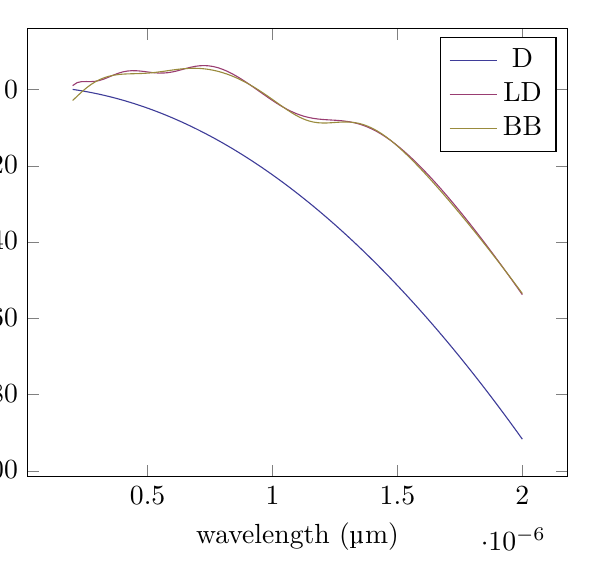
\begin{tikzpicture}[baseline,trim axis left]
\begin{axis}[xlabel=wavelength (\si{\micro\meter}),ylabel=$\epsilon'$]
\addplot[color=colora] coordinates {
(2e-07, 0.0632769706569)
(2.18181818182e-07, -0.114755238014)
(2.36363636364e-07, -0.30826032763)
(2.54545454545e-07, -0.517236253655)
(2.72727272727e-07, -0.741680808242)
(2.90909090909e-07, -0.981591620291)
(3.09090909091e-07, -1.23696615551)
(3.27272727273e-07, -1.5078017165)
(3.45454545455e-07, -1.79409544279)
(3.63636363636e-07, -2.09584431094)
(3.81818181818e-07, -2.41304513462)
(4e-07, -2.74569456468)
(4.18181818182e-07, -3.09378908927)
(4.36363636364e-07, -3.45732503386)
(4.54545454545e-07, -3.83629856145)
(4.72727272727e-07, -4.23070567255)
(4.90909090909e-07, -4.64054220537)
(5.09090909091e-07, -5.06580383591)
(5.27272727273e-07, -5.50648607805)
(5.45454545455e-07, -5.96258428369)
(5.63636363636e-07, -6.43409364287)
(5.81818181818e-07, -6.92100918389)
(6e-07, -7.42332577344)
(6.18181818182e-07, -7.94103811675)
(6.36363636364e-07, -8.47414075772)
(6.54545454545e-07, -9.02262807905)
(6.72727272727e-07, -9.58649430242)
(6.90909090909e-07, -10.1657334886)
(7.09090909091e-07, -10.7603395376)
(7.27272727273e-07, -11.370306189)
(7.45454545455e-07, -11.9956270218)
(7.63636363636e-07, -12.6362954548)
(7.81818181818e-07, -13.2923047469)
(8e-07, -13.9636479968)
(8.18181818182e-07, -14.6503181438)
(8.36363636364e-07, -15.3523079675)
(8.54545454545e-07, -16.0696100883)
(8.72727272727e-07, -16.8022169673)
(8.90909090909e-07, -17.5501209067)
(9.09090909091e-07, -18.3133140501)
(9.27272727273e-07, -19.0917883825)
(9.45454545455e-07, -19.8855357303)
(9.63636363636e-07, -20.6945477623)
(9.81818181818e-07, -21.518815989)
(1e-06, -22.3583317635)
(1.01818181818e-06, -23.2130862811)
(1.03636363636e-06, -24.0830705803)
(1.05454545455e-06, -24.9682755423)
(1.07272727273e-06, -25.8686918919)
(1.09090909091e-06, -26.7843101969)
(1.10909090909e-06, -27.7151208693)
(1.12727272727e-06, -28.661114165)
(1.14545454545e-06, -29.6222801839)
(1.16363636364e-06, -30.5986088707)
(1.18181818182e-06, -31.5900900147)
(1.2e-06, -32.5967132503)
(1.21818181818e-06, -33.6184680573)
(1.23636363636e-06, -34.6553437608)
(1.25454545455e-06, -35.7073295321)
(1.27272727273e-06, -36.7744143883)
(1.29090909091e-06, -37.8565871932)
(1.30909090909e-06, -38.9538366572)
(1.32727272727e-06, -40.0661513377)
(1.34545454545e-06, -41.1935196393)
(1.36363636364e-06, -42.3359298144)
(1.38181818182e-06, -43.4933699632)
(1.4e-06, -44.6658280341)
(1.41818181818e-06, -45.853291824)
(1.43636363636e-06, -47.0557489787)
(1.45454545455e-06, -48.2731869932)
(1.47272727273e-06, -49.5055932119)
(1.49090909091e-06, -50.752954829)
(1.50909090909e-06, -52.0152588889)
(1.52727272727e-06, -53.2924922863)
(1.54545454545e-06, -54.584641767)
(1.56363636364e-06, -55.8916939278)
(1.58181818182e-06, -57.2136352169)
(1.6e-06, -58.5504519344)
(1.61818181818e-06, -59.9021302327)
(1.63636363636e-06, -61.2686561166)
(1.65454545455e-06, -62.650015444)
(1.67272727273e-06, -64.0461939259)
(1.69090909091e-06, -65.457177127)
(1.70909090909e-06, -66.8829504659)
(1.72727272727e-06, -68.3234992157)
(1.74545454545e-06, -69.7788085043)
(1.76363636364e-06, -71.2488633146)
(1.78181818182e-06, -72.7336484852)
(1.8e-06, -74.2331487103)
(1.81818181818e-06, -75.7473485407)
(1.83636363636e-06, -77.2762323838)
(1.85454545455e-06, -78.8197845039)
(1.87272727273e-06, -80.3779890231)
(1.89090909091e-06, -81.9508299211)
(1.90909090909e-06, -83.5382910361)
(1.92727272727e-06, -85.1403560649)
(1.94545454545e-06, -86.7570085635)
(1.96363636364e-06, -88.3882319472)
(1.98181818182e-06, -90.0340094916)
(2e-06, -91.6943243325)
};
\addlegendentry{D}
\addplot[color=colorb] coordinates {
(2e-07, 1.05507401931)
(2.18181818182e-07, 1.85361373256)
(2.36363636364e-07, 2.11263249445)
(2.54545454545e-07, 2.12475241374)
(2.72727272727e-07, 2.10743441346)
(2.90909090909e-07, 2.19292087922)
(3.09090909091e-07, 2.43700846254)
(3.27272727273e-07, 2.83081796818)
(3.45454545455e-07, 3.31968040955)
(3.63636363636e-07, 3.82858075198)
(3.81818181818e-07, 4.28664265182)
(4e-07, 4.64312704439)
(4.18181818182e-07, 4.87286629118)
(4.36363636364e-07, 4.9740321294)
(4.54545454545e-07, 4.96254566698)
(4.72727272727e-07, 4.86620571072)
(4.90909090909e-07, 4.71978192097)
(5.09090909091e-07, 4.56104501135)
(5.27272727273e-07, 4.42718186747)
(5.45454545455e-07, 4.35108596973)
(5.63636363636e-07, 4.35741486937)
(5.81818181818e-07, 4.45887397047)
(6e-07, 4.65366866045)
(6.18181818182e-07, 4.9251612072)
(6.36363636364e-07, 5.24428450402)
(6.54545454545e-07, 5.57434081959)
(6.72727272727e-07, 5.87692944617)
(6.90909090909e-07, 6.11741143719)
(7.09090909091e-07, 6.26868479301)
(7.27272727273e-07, 6.31281999722)
(7.45454545455e-07, 6.24083690509)
(7.63636363636e-07, 6.05129584388)
(7.81818181818e-07, 5.74840702985)
(8e-07, 5.34017893799)
(8.18181818182e-07, 4.83689019832)
(8.36363636364e-07, 4.2499786885)
(8.54545454545e-07, 3.59132489069)
(8.72727272727e-07, 2.87285359261)
(8.90909090909e-07, 2.10636558199)
(9.09090909091e-07, 1.303518579)
(9.27272727273e-07, 0.475890791522)
(9.45454545455e-07, -0.364925887551)
(9.63636363636e-07, -1.2072455806)
(9.81818181818e-07, -2.03925646976)
(1e-06, -2.8490676956)
(1.01818181818e-06, -3.6248609526)
(1.03636363636e-06, -4.35516602859)
(1.05454545455e-06, -5.0292688704)
(1.07272727273e-06, -5.63774447639)
(1.09090909091e-06, -6.17308481503)
(1.10909090909e-06, -6.63036602984)
(1.12727272727e-06, -7.00787411963)
(1.14545454545e-06, -7.307591195)
(1.16363636364e-06, -7.53544319998)
(1.18181818182e-06, -7.70123041449)
(1.2e-06, -7.81820448282)
(1.21818181818e-06, -7.90231314299)
(1.23636363636e-06, -7.97119280618)
(1.25454545455e-06, -8.04303390893)
(1.27272727273e-06, -8.1354623284)
(1.29090909091e-06, -8.26456816447)
(1.30909090909e-06, -8.44417631991)
(1.32727272727e-06, -8.68540363635)
(1.34545454545e-06, -8.99649851189)
(1.36363636364e-06, -9.38292144019)
(1.38181818182e-06, -9.84760371036)
(1.4e-06, -10.3913161416)
(1.41818181818e-06, -11.0130862427)
(1.43636363636e-06, -11.7106154125)
(1.45454545455e-06, -12.4806631002)
(1.47272727273e-06, -13.3193789911)
(1.49090909091e-06, -14.2225755793)
(1.50909090909e-06, -15.1859414524)
(1.52727272727e-06, -16.2052005086)
(1.54545454545e-06, -17.2762248087)
(1.56363636364e-06, -18.3951095294)
(1.58181818182e-06, -19.5582181733)
(1.6e-06, -20.7622052896)
(1.61818181818e-06, -22.004022814)
(1.63636363636e-06, -23.2809149578)
(1.65454545455e-06, -24.5904054953)
(1.67272727273e-06, -25.930280358)
(1.69090909091e-06, -27.298567676)
(1.70909090909e-06, -28.6935167939)
(1.72727272727e-06, -30.1135773119)
(1.74545454545e-06, -31.557378848)
(1.76363636364e-06, -33.0237119531)
(1.78181818182e-06, -34.5115104196)
(1.8e-06, -36.0198350944)
(1.81818181818e-06, -37.5478592126)
(1.83636363636e-06, -39.0948552117)
(1.85454545455e-06, -40.6601829461)
(1.87272727273e-06, -42.2432792051)
(1.89090909091e-06, -43.8436484214)
(1.90909090909e-06, -45.4608544614)
(1.92727272727e-06, -47.0945133857)
(1.94545454545e-06, -48.7442870768)
(1.96363636364e-06, -50.4098776374)
(1.98181818182e-06, -52.0910224701)
(2e-06, -53.7874899594)
};
\addlegendentry{LD}
\addplot[color=colorc] coordinates {
(2e-07, -2.8458706636)
(2.18181818182e-07, -1.71289723129)
(2.36363636364e-07, -0.598094936076)
(2.54545454545e-07, 0.423092585504)
(2.72727272727e-07, 1.31464032329)
(2.90909090909e-07, 2.06467788373)
(3.09090909091e-07, 2.67504523329)
(3.27272727273e-07, 3.15498844463)
(3.45454545455e-07, 3.51771798041)
(3.63636363636e-07, 3.77875024036)
(3.81818181818e-07, 3.9552424574)
(4e-07, 4.06572710845)
(4.18181818182e-07, 4.12977440858)
(4.36363636364e-07, 4.16725233333)
(4.54545454545e-07, 4.19707995677)
(4.72727272727e-07, 4.2356477828)
(4.90909090909e-07, 4.29528683895)
(5.09090909091e-07, 4.38320002635)
(5.27272727273e-07, 4.50112132531)
(5.45454545455e-07, 4.64573494601)
(5.63636363636e-07, 4.80968300038)
(5.81818181818e-07, 4.98288597626)
(6e-07, 5.15390060195)
(6.18181818182e-07, 5.31110878636)
(6.36363636364e-07, 5.44362419697)
(6.54545454545e-07, 5.54188630063)
(6.72727272727e-07, 5.59796946441)
(6.90909090909e-07, 5.60566511487)
(7.09090909091e-07, 5.56040369792)
(7.27272727273e-07, 5.45907820923)
(7.45454545455e-07, 5.29981942837)
(7.63636363636e-07, 5.0817596727)
(7.81818181818e-07, 4.80480979834)
(8e-07, 4.46946464802)
(8.18181818182e-07, 4.0766455143)
(8.36363636364e-07, 3.62758427579)
(8.54545454545e-07, 3.1237523079)
(8.72727272727e-07, 2.5668376949)
(8.90909090909e-07, 1.95877634333)
(9.09090909091e-07, 1.30184592884)
(9.27272727273e-07, 0.598835475191)
(9.45454545455e-07, -0.146693835046)
(9.63636363636e-07, -0.930042510637)
(9.81818181818e-07, -1.74489832588)
(1e-06, -2.58277832738)
(1.01818181818e-06, -3.4324607965)
(1.03636363636e-06, -4.27954664379)
(1.05454545455e-06, -5.10635322173)
(1.07272727273e-06, -5.89236916321)
(1.09090909091e-06, -6.61544776536)
(1.10909090909e-06, -7.25377020739)
(1.12727272727e-06, -7.78839237795)
(1.14545454545e-06, -8.20596877701)
(1.16363636364e-06, -8.50111162783)
(1.18181818182e-06, -8.67785813308)
(1.2e-06, -8.7498921091)
(1.21818181818e-06, -8.73944388198)
(1.23636363636e-06, -8.67508284031)
(1.25454545455e-06, -8.58883193859)
(1.27272727273e-06, -8.51312082093)
(1.29090909091e-06, -8.47805113174)
(1.30909090909e-06, -8.50931056767)
(1.32727272727e-06, -8.62689576513)
(1.34545454545e-06, -8.84463882834)
(1.36363636364e-06, -9.17041129136)
(1.38181818182e-06, -9.60681461645)
(1.4e-06, -10.1521530038)
(1.41818181818e-06, -10.8015077715)
(1.43636363636e-06, -11.5477758548)
(1.45454545455e-06, -12.3825834798)
(1.47272727273e-06, -13.2970298673)
(1.49090909091e-06, -14.2822497969)
(1.50909090909e-06, -15.329806712)
(1.52727272727e-06, -16.4319408796)
(1.54545454545e-06, -17.5817021895)
(1.56363636364e-06, -18.7729969835)
(1.58181818182e-06, -20.0005750424)
(1.6e-06, -21.2599782022)
(1.61818181818e-06, -22.5474671512)
(1.63636363636e-06, -23.8599384428)
(1.65454545455e-06, -25.1948399635)
(1.67272727273e-06, -26.5500901027)
(1.69090909091e-06, -27.9240036509)
(1.70909090909e-06, -29.315225874)
(1.72727272727e-06, -30.7226751622)
(1.74545454545e-06, -32.1454939879)
(1.76363636364e-06, -33.5830075293)
(1.78181818182e-06, -35.0346891325)
(1.8e-06, -36.5001317269)
(1.81818181818e-06, -37.9790243308)
(1.83636363636e-06, -39.4711328475)
(1.85454545455e-06, -40.976284442)
(1.87272727273e-06, -42.4943548754)
(1.89090909091e-06, -44.0252582729)
(1.90909090909e-06, -45.5689388772)
(1.92727272727e-06, -47.1253644191)
(1.94545454545e-06, -48.6945208)
(1.96363636364e-06, -50.2764078346)
(1.98181818182e-06, -51.8710358506)
(2e-06, -53.4784229789)
};
\addlegendentry{BB}
\end{axis}
\end{tikzpicture}%
\\
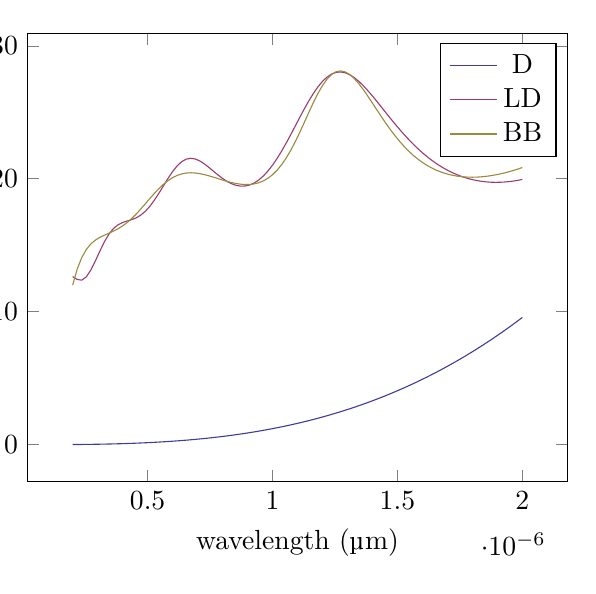
\begin{tikzpicture}[baseline,trim axis left]
\begin{axis}[xlabel=wavelength (\si{\micro\meter}),ylabel=$\epsilon''$]
\addplot[color=colora] coordinates {
(2e-07, 0.0096706317904)
(2.18181818182e-07, 0.0125548559147)
(2.36363636364e-07, 0.0159620434736)
(2.54545454545e-07, 0.0199357331734)
(2.72727272727e-07, 0.0245194537455)
(2.90909090909e-07, 0.0297567231814)
(3.09090909091e-07, 0.0356910479675)
(3.27272727273e-07, 0.0423659223203)
(3.45454545455e-07, 0.0498248274222)
(3.63636363636e-07, 0.058111230658)
(3.81818181818e-07, 0.0672685848515)
(4e-07, 0.0773403275027)
(4.18181818182e-07, 0.0883698800259)
(4.36363636364e-07, 0.100400646988)
(4.54545454545e-07, 0.113476015348)
(4.72727272727e-07, 0.127639353697)
(4.90909090909e-07, 0.142934011496)
(5.09090909091e-07, 0.159403318321)
(5.27272727273e-07, 0.177090583103)
(5.45454545455e-07, 0.196039093369)
(5.63636363636e-07, 0.216292114489)
(5.81818181818e-07, 0.237892888917)
(6e-07, 0.260884635438)
(6.18181818182e-07, 0.285310548412)
(6.36363636364e-07, 0.311213797024)
(6.54545454545e-07, 0.338637524529)
(6.72727272727e-07, 0.367624847501)
(6.90909090909e-07, 0.398218855085)
(7.09090909091e-07, 0.430462608243)
(7.27272727273e-07, 0.464399139014)
(7.45454545455e-07, 0.500071449756)
(7.63636363636e-07, 0.537522512409)
(7.81818181818e-07, 0.576795267746)
(8e-07, 0.61793262463)
(8.18181818182e-07, 0.660977459269)
(8.36363636364e-07, 0.70597261448)
(8.54545454545e-07, 0.752960898942)
(8.72727272727e-07, 0.801985086464)
(8.90909090909e-07, 0.853087915241)
(9.09090909091e-07, 0.906312087121)
(9.27272727273e-07, 0.96170026687)
(9.45454545455e-07, 1.01929508144)
(9.63636363636e-07, 1.07913911922)
(9.81818181818e-07, 1.14127492935)
(1e-06, 1.20574502092)
(1.01818181818e-06, 1.27259186232)
(1.03636363636e-06, 1.34185788046)
(1.05454545455e-06, 1.41358546005)
(1.07272727273e-06, 1.48781694291)
(1.09090909091e-06, 1.56459462721)
(1.10909090909e-06, 1.64396076678)
(1.12727272727e-06, 1.72595757036)
(1.14545454545e-06, 1.81062720091)
(1.16363636364e-06, 1.89801177489)
(1.18181818182e-06, 1.98815336152)
(1.2e-06, 2.08109398211)
(1.21818181818e-06, 2.17687560932)
(1.23636363636e-06, 2.27554016645)
(1.25454545455e-06, 2.37712952677)
(1.27272727273e-06, 2.48168551276)
(1.29090909091e-06, 2.58924989546)
(1.30909090909e-06, 2.69986439371)
(1.32727272727e-06, 2.81357067353)
(1.34545454545e-06, 2.93041034734)
(1.36363636364e-06, 3.05042497332)
(1.38181818182e-06, 3.17365605469)
(1.4e-06, 3.30014503905)
(1.41818181818e-06, 3.42993331762)
(1.43636363636e-06, 3.56306222466)
(1.45454545455e-06, 3.69957303667)
(1.47272727273e-06, 3.83950697181)
(1.49090909091e-06, 3.98290518912)
(1.50909090909e-06, 4.12980878794)
(1.52727272727e-06, 4.28025880715)
(1.54545454545e-06, 4.43429622454)
(1.56363636364e-06, 4.59196195614)
(1.58181818182e-06, 4.75329685552)
(1.6e-06, 4.91834171314)
(1.61818181818e-06, 5.08713725568)
(1.63636363636e-06, 5.2597241454)
(1.65454545455e-06, 5.43614297942)
(1.67272727273e-06, 5.61643428915)
(1.69090909091e-06, 5.80063853953)
(1.70909090909e-06, 5.98879612846)
(1.72727272727e-06, 6.18094738611)
(1.74545454545e-06, 6.37713257427)
(1.76363636364e-06, 6.5773918857)
(1.78181818182e-06, 6.78176544353)
(1.8e-06, 6.99029330055)
(1.81818181818e-06, 7.20301543861)
(1.83636363636e-06, 7.41997176799)
(1.85454545455e-06, 7.64120212673)
(1.87272727273e-06, 7.86674628003)
(1.89090909091e-06, 8.09664391963)
(1.90909090909e-06, 8.33093466313)
(1.92727272727e-06, 8.56965805342)
(1.94545454545e-06, 8.81285355802)
(1.96363636364e-06, 9.06056056851)
(1.98181818182e-06, 9.31281839985)
(2e-06, 9.56966628981)
};
\addlegendentry{D}
\addplot[color=colorb] coordinates {
(2e-07, 12.6422278445)
(2.18181818182e-07, 12.4261631985)
(2.36363636364e-07, 12.3739247824)
(2.54545454545e-07, 12.6168903938)
(2.72727272727e-07, 13.1296040441)
(2.90909090909e-07, 13.8182474887)
(3.09090909091e-07, 14.5664103166)
(3.27272727273e-07, 15.2664407832)
(3.45454545455e-07, 15.8430602201)
(3.63636363636e-07, 16.2648912522)
(3.81818181818e-07, 16.5415234946)
(4e-07, 16.7104812314)
(4.18181818182e-07, 16.8216883769)
(4.36363636364e-07, 16.9250454231)
(4.54545454545e-07, 17.062872026)
(4.72727272727e-07, 17.266310748)
(4.90909090909e-07, 17.5540052111)
(5.09090909091e-07, 17.9317422186)
(5.27272727273e-07, 18.3924902172)
(5.45454545455e-07, 18.9169392318)
(5.63636363636e-07, 19.4750559523)
(5.81818181818e-07, 20.0291958098)
(6e-07, 20.5389070286)
(6.18181818182e-07, 20.9668333345)
(6.36363636364e-07, 21.2844243356)
(6.54545454545e-07, 21.4759465182)
(6.72727272727e-07, 21.5397754584)
(6.90909090909e-07, 21.4869104194)
(7.09090909091e-07, 21.3375502765)
(7.27272727273e-07, 21.1169701314)
(7.45454545455e-07, 20.851780611)
(7.63636363636e-07, 20.567183488)
(7.81818181818e-07, 20.285359842)
(8e-07, 20.0248150421)
(8.18181818182e-07, 19.8003822788)
(8.36363636364e-07, 19.6235946741)
(8.54545454545e-07, 19.5032038664)
(8.72727272727e-07, 19.4457006431)
(8.90909090909e-07, 19.4557568657)
(9.09090909091e-07, 19.5365516339)
(9.27272727273e-07, 19.6899711161)
(9.45454545455e-07, 19.916686162)
(9.63636363636e-07, 20.2161199136)
(9.81818181818e-07, 20.5863231383)
(1e-06, 21.0237805638)
(1.01818181818e-06, 21.5231785083)
(1.03636363636e-06, 22.0771727784)
(1.05454545455e-06, 22.6762050669)
(1.07272727273e-06, 23.3084235258)
(1.09090909091e-06, 23.9597652254)
(1.10909090909e-06, 24.6142507353)
(1.12727272727e-06, 25.2545207849)
(1.14545454545e-06, 25.8626111945)
(1.16363636364e-06, 26.420918722)
(1.18181818182e-06, 26.9132657518)
(1.2e-06, 27.3259379314)
(1.21818181818e-06, 27.648557578)
(1.23636363636e-06, 27.8746734486)
(1.25454545455e-06, 28.0019920612)
(1.27272727273e-06, 28.0322362073)
(1.29090909091e-06, 27.9706766588)
(1.30909090909e-06, 27.825428395)
(1.32727272727e-06, 27.6066241348)
(1.34545454545e-06, 27.3255748595)
(1.36363636364e-06, 26.994005398)
(1.38181818182e-06, 26.6234222371)
(1.4e-06, 26.2246393008)
(1.41818181818e-06, 25.8074616096)
(1.43636363636e-06, 25.3805092112)
(1.45454545455e-06, 24.9511545663)
(1.47272727273e-06, 24.5255440509)
(1.49090909091e-06, 24.1086761882)
(1.50909090909e-06, 23.7045135934)
(1.52727272727e-06, 23.3161108188)
(1.54545454545e-06, 22.9457453207)
(1.56363636364e-06, 22.5950430866)
(1.58181818182e-06, 22.2650938713)
(1.6e-06, 21.9565535034)
(1.61818181818e-06, 21.6697324642)
(1.63636363636e-06, 21.4046710603)
(1.65454545455e-06, 21.1612021745)
(1.67272727273e-06, 20.9390029127)
(1.69090909091e-06, 20.7376365856)
(1.70909090909e-06, 20.5565864448)
(1.72727272727e-06, 20.3952824938)
(1.74545454545e-06, 20.2531225603)
(1.76363636364e-06, 20.1294886624)
(1.78181818182e-06, 20.0237595529)
(1.8e-06, 19.9353201836)
(1.81818181818e-06, 19.8635687088)
(1.83636363636e-06, 19.8079215356)
(1.85454545455e-06, 19.7678168359)
(1.87272727273e-06, 19.7427168578)
(1.89090909091e-06, 19.7321093052)
(1.90909090909e-06, 19.7355080043)
(1.92727272727e-06, 19.7524530292)
(1.94545454545e-06, 19.7825104239)
(1.96363636364e-06, 19.8252716284)
(1.98181818182e-06, 19.8803526948)
(2e-06, 19.947393358)
};
\addlegendentry{LD}
\addplot[color=colorc] coordinates {
(2e-07, 11.9972071613)
(2.18181818182e-07, 13.200908114)
(2.36363636364e-07, 14.0687937291)
(2.54545454545e-07, 14.6766231677)
(2.72727272727e-07, 15.0957925959)
(2.90909090909e-07, 15.386051821)
(3.09090909091e-07, 15.5948551831)
(3.27272727273e-07, 15.7591280161)
(3.45454545455e-07, 15.9074824921)
(3.63636363636e-07, 16.06207015)
(3.81818181818e-07, 16.2397791754)
(4e-07, 16.4527285998)
(4.18181818182e-07, 16.7081848203)
(4.36363636364e-07, 17.0081965828)
(4.54545454545e-07, 17.3493626799)
(4.72727272727e-07, 17.72311885)
(4.90909090909e-07, 18.1167314063)
(5.09090909091e-07, 18.5149039135)
(5.27272727273e-07, 18.9016802267)
(5.45454545455e-07, 19.2622542612)
(5.63636363636e-07, 19.5843720415)
(5.81818181818e-07, 19.8591669705)
(6e-07, 20.0814267241)
(6.18181818182e-07, 20.249399855)
(6.36363636364e-07, 20.3642985677)
(6.54545454545e-07, 20.4296526618)
(6.72727272727e-07, 20.4506390732)
(6.90909090909e-07, 20.4334708017)
(7.09090909091e-07, 20.3848909354)
(7.27272727273e-07, 20.3117880375)
(7.45454545455e-07, 20.2209296934)
(7.63636363636e-07, 20.1188002547)
(7.81818181818e-07, 20.0115244957)
(8e-07, 19.9048587447)
(8.18181818182e-07, 19.804233179)
(8.36363636364e-07, 19.714832013)
(8.54545454545e-07, 19.6417013156)
(8.72727272727e-07, 19.5898764519)
(8.90909090909e-07, 19.5645220111)
(9.09090909091e-07, 19.5710757484)
(9.27272727273e-07, 19.6153834095)
(9.45454545455e-07, 19.7038019223)
(9.63636363636e-07, 19.8432332154)
(9.81818181818e-07, 20.041030511)
(1e-06, 20.304698372)
(1.01818181818e-06, 20.6412989257)
(1.03636363636e-06, 21.0564977967)
(1.05454545455e-06, 21.5532518822)
(1.07272727273e-06, 22.1302602992)
(1.09090909091e-06, 22.7804444937)
(1.10909090909e-06, 23.4898390077)
(1.12727272727e-06, 24.2372958499)
(1.14545454545e-06, 24.9952919403)
(1.16363636364e-06, 25.7318931808)
(1.18181818182e-06, 26.413639714)
(1.2e-06, 27.0088733209)
(1.21818181818e-06, 27.4909130772)
(1.23636363636e-06, 27.8405321562)
(1.25454545455e-06, 28.0473701897)
(1.27272727273e-06, 28.1101636454)
(1.29090909091e-06, 28.0359135964)
(1.30909090909e-06, 27.8382776899)
(1.32727272727e-06, 27.5355461597)
(1.34545454545e-06, 27.1485474332)
(1.36363636364e-06, 26.6987545353)
(1.38181818182e-06, 26.2067624492)
(1.4e-06, 25.6912073592)
(1.41818181818e-06, 25.168119441)
(1.43636363636e-06, 24.6506489758)
(1.45454545455e-06, 24.1490801501)
(1.47272727273e-06, 23.6710423352)
(1.49090909091e-06, 23.2218377159)
(1.50909090909e-06, 22.8048201741)
(1.52727272727e-06, 22.42177826)
(1.54545454545e-06, 22.0732916557)
(1.56363636364e-06, 21.7590441113)
(1.58181818182e-06, 21.4780859145)
(1.6e-06, 21.2290457757)
(1.61818181818e-06, 21.0102961253)
(1.63636363636e-06, 20.8200779211)
(1.65454545455e-06, 20.6565917661)
(1.67272727273e-06, 20.5180619681)
(1.69090909091e-06, 20.4027795168)
(1.70909090909e-06, 20.3091290829)
(1.72727272727e-06, 20.235604231)
(1.74545454545e-06, 20.1808141773)
(1.76363636364e-06, 20.1434846725)
(1.78181818182e-06, 20.1224549594)
(1.8e-06, 20.1166722488)
(1.81818181818e-06, 20.1251847518)
(1.83636363636e-06, 20.1471340083)
(1.85454545455e-06, 20.1817470128)
(1.87272727273e-06, 20.2283284739)
(1.89090909091e-06, 20.2862534182)
(1.90909090909e-06, 20.3549602625)
(1.92727272727e-06, 20.4339444161)
(1.94545454545e-06, 20.522752436)
(1.96363636364e-06, 20.6209767271)
(1.98181818182e-06, 20.7282507669)
(2e-06, 20.8442448186)
};
\addlegendentry{BB}
\end{axis}
\end{tikzpicture}%
\\
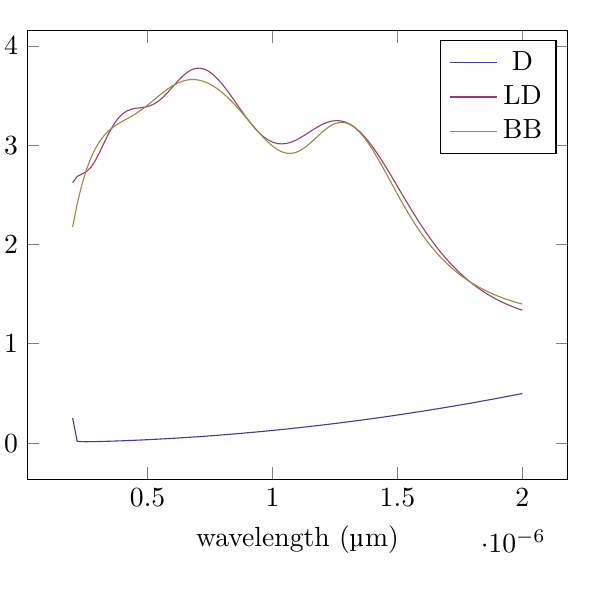
\begin{tikzpicture}[baseline,trim axis left]
\begin{axis}[xlabel=wavelength (\si{\micro\meter}),ylabel=$n'$]
\addplot[color=colora] coordinates {
(2e-07, 0.25227827705)
(2.18181818182e-07, 0.0185032742565)
(2.36363636364e-07, 0.0143699171419)
(2.54545454545e-07, 0.0138572527108)
(2.72727272727e-07, 0.0142335413547)
(2.90909090909e-07, 0.0150155006291)
(3.09090909091e-07, 0.0160437251798)
(3.27272727273e-07, 0.017249309202)
(3.45454545455e-07, 0.0185973548944)
(3.63636363636e-07, 0.0200682196386)
(3.81818181818e-07, 0.021649974916)
(4e-07, 0.023334948098)
(4.18181818182e-07, 0.0251179759281)
(4.36363636364e-07, 0.0269954544958)
(4.54545454545e-07, 0.0289647910279)
(4.72727272727e-07, 0.0310240719293)
(4.90909090909e-07, 0.033171853542)
(5.09090909091e-07, 0.0354070257026)
(5.27272727273e-07, 0.0377287201412)
(5.45454545455e-07, 0.0401362474133)
(5.63636363636e-07, 0.0426290525039)
(5.81818181818e-07, 0.04520668296)
(6e-07, 0.0478687656137)
(6.18181818182e-07, 0.0506149893131)
(6.36363636364e-07, 0.0534450919301)
(6.54545454545e-07, 0.0563588504587)
(6.72727272727e-07, 0.0593560733828)
(6.90909090909e-07, 0.0624365947287)
(7.09090909091e-07, 0.0656002693871)
(7.27272727273e-07, 0.0688469693984)
(7.45454545455e-07, 0.0721765809801)
(7.63636363636e-07, 0.0755890021292)
(7.81818181818e-07, 0.0790841406734)
(8e-07, 0.0826619126789)
(8.18181818182e-07, 0.0863222411389)
(8.36363636364e-07, 0.0900650548884)
(8.54545454545e-07, 0.0938902877015)
(8.72727272727e-07, 0.0977978775356)
(8.90909090909e-07, 0.101787765896)
(9.09090909091e-07, 0.105859897302)
(9.27272727273e-07, 0.110014218826)
(9.45454545455e-07, 0.114250679715)
(9.63636363636e-07, 0.118569231053)
(9.81818181818e-07, 0.122969825477)
(1e-06, 0.127452416936)
(1.01818181818e-06, 0.132016960478)
(1.03636363636e-06, 0.136663412066)
(1.05454545455e-06, 0.14139172842)
(1.07272727273e-06, 0.146201866877)
(1.09090909091e-06, 0.151093785272)
(1.10909090909e-06, 0.156067441829)
(1.12727272727e-06, 0.16112279507)
(1.14545454545e-06, 0.166259803731)
(1.16363636364e-06, 0.171478426691)
(1.18181818182e-06, 0.176778622907)
(1.2e-06, 0.182160351357)
(1.21818181818e-06, 0.18762357099)
(1.23636363636e-06, 0.193168240682)
(1.25454545455e-06, 0.198794319193)
(1.27272727273e-06, 0.204501765135)
(1.29090909091e-06, 0.210290536938)
(1.30909090909e-06, 0.216160592822)
(1.32727272727e-06, 0.22211189077)
(1.34545454545e-06, 0.228144388507)
(1.36363636364e-06, 0.234258043479)
(1.38181818182e-06, 0.240452812835)
(1.4e-06, 0.246728653406)
(1.41818181818e-06, 0.253085521697)
(1.43636363636e-06, 0.259523373866)
(1.45454545455e-06, 0.266042165719)
(1.47272727273e-06, 0.272641852693)
(1.49090909091e-06, 0.279322389848)
(1.50909090909e-06, 0.286083731859)
(1.52727272727e-06, 0.292925833007)
(1.54545454545e-06, 0.299848647172)
(1.56363636364e-06, 0.306852127823)
(1.58181818182e-06, 0.313936228019)
(1.6e-06, 0.321100900396)
(1.61818181818e-06, 0.328346097168)
(1.63636363636e-06, 0.335671770116)
(1.65454545455e-06, 0.343077870593)
(1.67272727273e-06, 0.350564349512)
(1.69090909091e-06, 0.358131157345)
(1.70909090909e-06, 0.365778244124)
(1.72727272727e-06, 0.373505559433)
(1.74545454545e-06, 0.38131305241)
(1.76363636364e-06, 0.389200671742)
(1.78181818182e-06, 0.397168365664)
(1.8e-06, 0.405216081957)
(1.81818181818e-06, 0.413343767948)
(1.83636363636e-06, 0.421551370507)
(1.85454545455e-06, 0.429838836049)
(1.87272727273e-06, 0.438206110526)
(1.89090909091e-06, 0.446653139437)
(1.90909090909e-06, 0.455179867817)
(1.92727272727e-06, 0.463786240241)
(1.94545454545e-06, 0.472472200827)
(1.96363636364e-06, 0.481237693228)
(1.98181818182e-06, 0.490082660639)
(2e-06, 0.499007045792)
};
\addlegendentry{D}
\addplot[color=colorb] coordinates {
(2e-07, 2.62118787722)
(2.18181818182e-07, 2.68488996839)
(2.36363636364e-07, 2.70791519948)
(2.54545454545e-07, 2.73123615598)
(2.72727272727e-07, 2.77534639201)
(2.90909090909e-07, 2.84465216398)
(3.09090909091e-07, 2.93307617076)
(3.27272727273e-07, 3.02964490049)
(3.45454545455e-07, 3.12304337392)
(3.63636363636e-07, 3.20452810804)
(3.81818181818e-07, 3.26914142233)
(4e-07, 3.31562056776)
(4.18181818182e-07, 3.34560302122)
(4.36363636364e-07, 3.36265085784)
(4.54545454545e-07, 3.37138107996)
(4.72727272727e-07, 3.37676933397)
(4.90909090909e-07, 3.38357984202)
(5.09090909091e-07, 3.39586228478)
(5.27272727273e-07, 3.41650366041)
(5.45454545455e-07, 3.44688069823)
(5.63636363636e-07, 3.48668821681)
(5.81818181818e-07, 3.53400500722)
(6e-07, 3.58560925815)
(6.18181818182e-07, 3.63749184639)
(6.36363636364e-07, 3.68546209145)
(6.54545454545e-07, 3.7257173761)
(6.72727272727e-07, 3.75526617436)
(6.90909090909e-07, 3.77214675515)
(7.09090909091e-07, 3.77544746974)
(7.27272727273e-07, 3.76518225684)
(7.45454545455e-07, 3.74209275067)
(7.63636363636e-07, 3.70743942278)
(7.81818181818e-07, 3.66282162055)
(8e-07, 3.61004290498)
(8.18181818182e-07, 3.55102074308)
(8.36363636364e-07, 3.48772985931)
(8.54545454545e-07, 3.42216496598)
(8.72727272727e-07, 3.35630916585)
(8.90909090909e-07, 3.29209754274)
(9.09090909091e-07, 3.23137034637)
(9.27272727273e-07, 3.17581580206)
(9.45454545455e-07, 3.12690767318)
(9.63636363636e-07, 3.08584581454)
(9.81818181818e-07, 3.05350808492)
(1e-06, 3.03041930601)
(1.01818181818e-06, 3.01673885503)
(1.03636363636e-06, 3.01226483774)
(1.05454545455e-06, 3.0164509522)
(1.07272727273e-06, 3.02843237925)
(1.09090909091e-06, 3.04705863615)
(1.10909090909e-06, 3.07093323514)
(1.12727272727e-06, 3.09846126313)
(1.14545454545e-06, 3.1279061205)
(1.16363636364e-06, 3.15745556912)
(1.18181818182e-06, 3.1852952839)
(1.2e-06, 3.20968589416)
(1.21818181818e-06, 3.22903775025)
(1.23636363636e-06, 3.24197695142)
(1.25454545455e-06, 3.24739680348)
(1.27272727273e-06, 3.24449070837)
(1.29090909091e-06, 3.23276503618)
(1.30909090909e-06, 3.21203312971)
(1.32727272727e-06, 3.18239364556)
(1.34545454545e-06, 3.14419758456)
(1.36363636364e-06, 3.09800855573)
(1.38181818182e-06, 3.04456024941)
(1.4e-06, 2.98471409684)
(1.41818181818e-06, 2.91941900533)
(1.43636363636e-06, 2.84967414261)
(1.45454545455e-06, 2.77649514504)
(1.47272727273e-06, 2.70088386621)
(1.49090909091e-06, 2.62380179219)
(1.50909090909e-06, 2.54614739778)
(1.52727272727e-06, 2.4687378605)
(1.54545454545e-06, 2.3922955733)
(1.56363636364e-06, 2.31743975384)
(1.58181818182e-06, 2.24468315602)
(1.6e-06, 2.17443352498)
(1.61818181818e-06, 2.10699909149)
(1.63636363636e-06, 2.04259715767)
(1.65454545455e-06, 1.98136472153)
(1.67272727273e-06, 1.92337012318)
(1.69090909091e-06, 1.86862483698)
(1.70909090909e-06, 1.81709473523)
(1.72727272727e-06, 1.76871036467)
(1.74545454545e-06, 1.72337597558)
(1.76363636364e-06, 1.6809772037)
(1.78181818182e-06, 1.64138742308)
(1.8e-06, 1.60447286491)
(1.81818181818e-06, 1.57009663971)
(1.83636363636e-06, 1.53812181838)
(1.85454545455e-06, 1.50841372709)
(1.87272727273e-06, 1.48084160106)
(1.89090909091e-06, 1.4552797257)
(1.90909090909e-06, 1.43160817575)
(1.92727272727e-06, 1.4097132445)
(1.94545454545e-06, 1.3894876388)
(1.96363636364e-06, 1.37083050039)
(1.98181818182e-06, 1.35364730163)
(2e-06, 1.33784965305)
};
\addlegendentry{LD}
\addplot[color=colorc] coordinates {
(2e-07, 2.17764246414)
(2.18181818182e-07, 2.40818151083)
(2.36363636364e-07, 2.59647898226)
(2.54545454545e-07, 2.74825516189)
(2.72727272727e-07, 2.8694571378)
(2.90909090909e-07, 2.96552210896)
(3.09090909091e-07, 3.04118952824)
(3.27272727273e-07, 3.10055069967)
(3.45454545455e-07, 3.14718171164)
(3.63636363636e-07, 3.18428387002)
(3.81818181818e-07, 3.21478912829)
(4e-07, 3.24140128364)
(4.18181818182e-07, 3.26655576413)
(4.36363636364e-07, 3.29230368231)
(4.54545454545e-07, 3.32015768581)
(4.72727272727e-07, 3.35096086566)
(4.90909090909e-07, 3.38483683362)
(5.09090909091e-07, 3.42124746254)
(5.27272727273e-07, 3.45914334954)
(5.45454545455e-07, 3.49716368465)
(5.63636363636e-07, 3.53383703415)
(5.81818181818e-07, 3.56774738186)
(6e-07, 3.59764891565)
(6.18181818182e-07, 3.62252925189)
(6.36363636364e-07, 3.64163036695)
(6.54545454545e-07, 3.65443992893)
(6.72727272727e-07, 3.66066514522)
(6.90909090909e-07, 3.66019878723)
(7.09090909091e-07, 3.65308417545)
(7.27272727273e-07, 3.63948336567)
(7.45454545455e-07, 3.61965084682)
(7.63636363636e-07, 3.59391374917)
(7.81818181818e-07, 3.56265875828)
(8e-07, 3.52632549355)
(8.18181818182e-07, 3.48540590705)
(8.36363636364e-07, 3.4404491761)
(8.54545454545e-07, 3.39207150824)
(8.72727272727e-07, 3.34097016615)
(8.90909090909e-07, 3.28794077045)
(9.09090909091e-07, 3.23389645391)
(9.27272727273e-07, 3.17988660496)
(9.45454545455e-07, 3.12711161808)
(9.63636363636e-07, 3.07692818116)
(9.81818181818e-07, 3.03083731751)
(1e-06, 2.99044536182)
(1.01818181818e-06, 2.95738782722)
(1.03636363636e-06, 2.9332098933)
(1.05454545455e-06, 2.91920658186)
(1.07272727273e-06, 2.91623958896)
(1.09090909091e-06, 2.92456154743)
(1.10909090909e-06, 2.94368550342)
(1.12727272727e-06, 2.97233285244)
(1.14545454545e-06, 3.00847744482)
(1.16363636364e-06, 3.0494827087)
(1.18181818182e-06, 3.09230983036)
(1.2e-06, 3.1337636193)
(1.21818181818e-06, 3.17074030612)
(1.23636363636e-06, 3.20044667067)
(1.25454545455e-06, 3.22056951557)
(1.27272727273e-06, 3.22938540612)
(1.29090909091e-06, 3.22581034732)
(1.30909090909e-06, 3.2093962413)
(1.32727272727e-06, 3.18028510281)
(1.34545454545e-06, 3.13913336773)
(1.36363636364e-06, 3.0870179066)
(1.38181818182e-06, 3.0253334233)
(1.4e-06, 2.95568861336)
(1.41818181818e-06, 2.87980642077)
(1.43636363636e-06, 2.79943231652)
(1.45454545455e-06, 2.71625374056)
(1.47272727273e-06, 2.63183343077)
(1.49090909091e-06, 2.54755889526)
(1.50909090909e-06, 2.46460943161)
(1.52727272727e-06, 2.38394077344)
(1.54545454545e-06, 2.3062858683)
(1.56363636364e-06, 2.23216886043)
(1.58181818182e-06, 2.16192843904)
(1.6e-06, 2.09574649472)
(1.61818181818e-06, 2.03367844239)
(1.63636363636e-06, 1.97568239416)
(1.65454545455e-06, 1.92164533153)
(1.67272727273e-06, 1.8714053194)
(1.69090909091e-06, 1.82476950273)
(1.70909090909e-06, 1.78152809711)
(1.72727272727e-06, 1.74146484904)
(1.74545454545e-06, 1.70436455101)
(1.76363636364e-06, 1.67001820195)
(1.78181818182e-06, 1.63822635087)
(1.8e-06, 1.60880108163)
(1.81818181818e-06, 1.58156701119)
(1.83636363636e-06, 1.55636159318)
(1.85454545455e-06, 1.53303494914)
(1.87272727273e-06, 1.51144939289)
(1.89090909091e-06, 1.49147876794)
(1.90909090909e-06, 1.47300768349)
(1.92727272727e-06, 1.45593070809)
(1.94545454545e-06, 1.44015156106)
(1.96363636364e-06, 1.42558232733)
(1.98181818182e-06, 1.41214271198)
(2e-06, 1.39975934317)
};
\addlegendentry{BB}
\end{axis}
\end{tikzpicture}%
\\
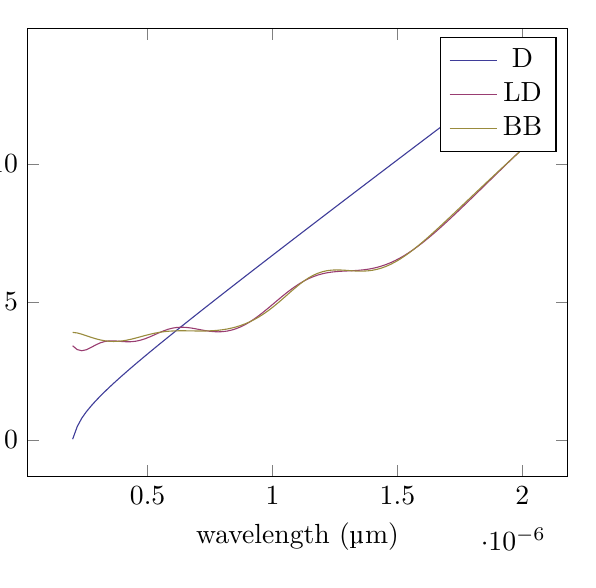
\begin{tikzpicture}[baseline,trim axis left]
\begin{axis}[xlabel=wavelength (\si{\micro\meter}),ylabel=$n''$]
\addplot[color=colora] coordinates {
(2e-07, 0.0271056604529)
(2.18181818182e-07, 0.479786638355)
(2.36363636364e-07, 0.785451236104)
(2.54545454545e-07, 1.01727899527)
(2.72727272727e-07, 1.21809966911)
(2.90909090909e-07, 1.40129731717)
(3.09090909091e-07, 1.5730375435)
(3.27272727273e-07, 1.73672061954)
(3.45454545455e-07, 1.89443464094)
(3.63636363636e-07, 2.04755807946)
(3.81818181818e-07, 2.1970497746)
(4e-07, 2.34360367148)
(4.18181818182e-07, 2.48773792912)
(4.36363636364e-07, 2.6298493449)
(4.54545454545e-07, 2.77024819125)
(4.72727272727e-07, 2.90918138506)
(4.90909090909e-07, 3.04684839703)
(5.09090909091e-07, 3.18341247512)
(5.27272727273e-07, 3.31900874792)
(5.45454545455e-07, 3.45375019422)
(5.63636363636e-07, 3.58773211904)
(5.81818181818e-07, 3.72103556233)
(6e-07, 3.85372993142)
(6.18181818182e-07, 3.98587505923)
(6.36363636364e-07, 4.11752283189)
(6.54545454545e-07, 4.24871848893)
(6.72727272727e-07, 4.37950167162)
(6.90909090909e-07, 4.50990727553)
(7.09090909091e-07, 4.63996614922)
(7.27272727273e-07, 4.76970567105)
(7.45454545455e-07, 4.89915022849)
(7.63636363636e-07, 5.028321619)
(7.81818181818e-07, 5.15723938715)
(8e-07, 5.28592110963)
(8.18181818182e-07, 5.41438263759)
(8.36363636364e-07, 5.54263830349)
(8.54545454545e-07, 5.67070109853)
(8.72727272727e-07, 5.79858282551)
(8.90909090909e-07, 5.92629423097)
(9.09090909091e-07, 6.05384511992)
(9.27272727273e-07, 6.18124445574)
(9.45454545455e-07, 6.30850044752)
(9.63636363636e-07, 6.43562062662)
(9.81818181818e-07, 6.56261191402)
(1e-06, 6.6894806797)
(1.01818181818e-06, 6.81623279517)
(1.03636363636e-06, 6.94287368004)
(1.05454545455e-06, 7.06940834345)
(1.07272727273e-06, 7.19584142095)
(1.09090909091e-06, 7.32217720748)
(1.10909090909e-06, 7.44841968685)
(1.12727272727e-06, 7.57457255824)
(1.14545454545e-06, 7.70063925999)
(1.16363636364e-06, 7.82662299098)
(1.18181818182e-06, 7.95252673007)
(1.2e-06, 8.07835325347)
(1.21818181818e-06, 8.20410515068)
(1.23636363636e-06, 8.32978483876)
(1.25454545455e-06, 8.45539457547)
(1.27272727273e-06, 8.58093647107)
(1.29090909091e-06, 8.70641249921)
(1.30909090909e-06, 8.83182450676)
(1.32727272727e-06, 8.9571742229)
(1.34545454545e-06, 9.08246326734)
(1.36363636364e-06, 9.20769315793)
(1.38181818182e-06, 9.33286531762)
(1.4e-06, 9.45798108081)
(1.41818181818e-06, 9.5830416993)
(1.43636363636e-06, 9.70804834767)
(1.45454545455e-06, 9.83300212826)
(1.47272727273e-06, 9.95790407583)
(1.49090909091e-06, 10.0827551618)
(1.50909090909e-06, 10.2075562982)
(1.52727272727e-06, 10.3323083413)
(1.54545454545e-06, 10.4570120951)
(1.56363636364e-06, 10.5816683142)
(1.58181818182e-06, 10.7062777072)
(1.6e-06, 10.830840939)
(1.61818181818e-06, 10.9553586333)
(1.63636363636e-06, 11.0798313754)
(1.65454545455e-06, 11.204259714)
(1.67272727273e-06, 11.3286441633)
(1.69090909091e-06, 11.452985205)
(1.70909090909e-06, 11.5772832901)
(1.72727272727e-06, 11.7015388406)
(1.74545454545e-06, 11.8257522508)
(1.76363636364e-06, 11.9499238891)
(1.78181818182e-06, 12.0740540993)
(1.8e-06, 12.1981432016)
(1.81818181818e-06, 12.3221914943)
(1.83636363636e-06, 12.4461992545)
(1.85454545455e-06, 12.5701667395)
(1.87272727273e-06, 12.6940941873)
(1.89090909091e-06, 12.8179818184)
(1.90909090909e-06, 12.9418298357)
(1.92727272727e-06, 13.0656384262)
(1.94545454545e-06, 13.1894077611)
(1.96363636364e-06, 13.3131379971)
(1.98181818182e-06, 13.4368292767)
(2e-06, 13.5604817292)
};
\addlegendentry{D}
\addplot[color=colorb] coordinates {
(2e-07, 3.41044040217)
(2.18181818182e-07, 3.27261987093)
(2.36363636364e-07, 3.23115218866)
(2.54545454545e-07, 3.26646552897)
(2.72727272727e-07, 3.34517957132)
(2.90909090909e-07, 3.43485809164)
(3.09090909091e-07, 3.51167406259)
(3.27272727273e-07, 3.56312510442)
(3.45454545455e-07, 3.58712127084)
(3.63636363636e-07, 3.5889886161)
(3.81818181818e-07, 3.57788847992)
(4e-07, 3.56376562219)
(4.18181818182e-07, 3.55533213201)
(4.36363636364e-07, 3.55904163009)
(4.54545454545e-07, 3.57873293761)
(4.72727272727e-07, 3.61562316181)
(4.90909090909e-07, 3.66846851598)
(5.09090909091e-07, 3.73385474968)
(5.27272727273e-07, 3.80665611636)
(5.45454545455e-07, 3.88069596286)
(5.63636363636e-07, 3.94957715505)
(5.81818181818e-07, 4.0075721879)
(6e-07, 4.05041358176)
(6.18181818182e-07, 4.07582770131)
(6.36363636364e-07, 4.08371064683)
(6.54545454545e-07, 4.07593649288)
(6.72727272727e-07, 4.05588328089)
(6.90909090909e-07, 4.02782316026)
(7.09090909091e-07, 3.99632801551)
(7.27272727273e-07, 3.96579813656)
(7.45454545455e-07, 3.94015767439)
(7.63636363636e-07, 3.92270601237)
(7.81818181818e-07, 3.91608355226)
(8e-07, 3.92230310858)
(8.18181818182e-07, 3.94280563038)
(8.36363636364e-07, 3.97851250671)
(8.54545454545e-07, 4.02986058412)
(8.72727272727e-07, 4.09681769772)
(8.90909090909e-07, 4.17888517404)
(9.09090909091e-07, 4.27509900152)
(9.27272727273e-07, 4.38404270442)
(9.45454545455e-07, 4.50388221075)
(9.63636363636e-07, 4.63242700358)
(9.81818181818e-07, 4.76721472024)
(1e-06, 4.90561084184)
(1.01818181818e-06, 5.04491313544)
(1.03636363636e-06, 5.18245221517)
(1.05454545455e-06, 5.31568344005)
(1.07272727273e-06, 5.44226922378)
(1.09090909091e-06, 5.56015308191)
(1.10909090909e-06, 5.66762683396)
(1.12727272727e-06, 5.763390724)
(1.14545454545e-06, 5.84660378231)
(1.16363636364e-06, 5.91691961597)
(1.18181818182e-06, 5.97450189725)
(1.2e-06, 6.02001462158)
(1.21818181818e-06, 6.05458469848)
(1.23636363636e-06, 6.07973804695)
(1.25454545455e-06, 6.09731414775)
(1.27272727273e-06, 6.10936695331)
(1.29090909091e-06, 6.11806144847)
(1.30909090909e-06, 6.12557477242)
(1.32727272727e-06, 6.13400895853)
(1.34545454545e-06, 6.14531967641)
(1.36363636364e-06, 6.16126260625)
(1.38181818182e-06, 6.18335682662)
(1.4e-06, 6.21286316951)
(1.41818181818e-06, 6.25077492338)
(1.43636363636e-06, 6.29781837329)
(1.45454545455e-06, 6.3544611716)
(1.47272727273e-06, 6.42092713708)
(1.49090909091e-06, 6.49721654618)
(1.50909090909e-06, 6.58313117349)
(1.52727272727e-06, 6.67830324746)
(1.54545454545e-06, 6.78222720332)
(1.56363636364e-06, 6.89429279071)
(1.58181818182e-06, 7.01381788246)
(1.6e-06, 7.14007933348)
(1.61818181818e-06, 7.27234047409)
(1.63636363636e-06, 7.40987423731)
(1.65454545455e-06, 7.55198141617)
(1.67272727273e-06, 7.69800402555)
(1.69090909091e-06, 7.84733412789)
(1.70909090909e-06, 7.99941873772)
(1.72727272727e-06, 8.15376154495)
(1.74545454545e-06, 8.30992221399)
(1.76363636364e-06, 8.46751395776)
(1.78181818182e-06, 8.62619998519)
(1.8e-06, 8.78568930347)
(1.81818181818e-06, 8.94573224176)
(1.83636363636e-06, 9.10611596015)
(1.85454545455e-06, 9.26666012306)
(1.87272727273e-06, 9.42721284925)
(1.89090909091e-06, 9.58764700033)
(1.90909090909e-06, 9.74785683423)
(1.92727272727e-06, 9.90775502497)
(1.94545454545e-06, 10.0672700346)
(1.96363636364e-06, 10.2263438137)
(1.98181818182e-06, 10.3849298011)
(2e-06, 10.5429911935)
};
\addlegendentry{LD}
\addplot[color=colorc] coordinates {
(2e-07, 3.89563791059)
(2.18181818182e-07, 3.87614123075)
(2.36363636364e-07, 3.83139610101)
(2.54545454545e-07, 3.77619222216)
(2.72727272727e-07, 3.71998493072)
(2.90909090909e-07, 3.66869009185)
(3.09090909091e-07, 3.62595877345)
(3.27272727273e-07, 3.59400228063)
(3.45454545455e-07, 3.57408302805)
(3.63636363636e-07, 3.56676703038)
(3.81818181818e-07, 3.57200970939)
(4e-07, 3.58913782771)
(4.18181818182e-07, 3.61679752034)
(4.36363636364e-07, 3.65294708508)
(4.54545454545e-07, 3.69496064982)
(4.72727272727e-07, 3.73986388532)
(4.90909090909e-07, 3.78466208565)
(5.09090909091e-07, 3.82667850063)
(5.27272727273e-07, 3.86381971302)
(5.45454545455e-07, 3.8947192174)
(5.63636363636e-07, 3.91875520632)
(5.81818181818e-07, 3.93597139331)
(6e-07, 3.94694239084)
(6.18181818182e-07, 3.95262176143)
(6.36363636364e-07, 3.95419967441)
(6.54545454545e-07, 3.95298492118)
(6.72727272727e-07, 3.95031640278)
(6.90909090909e-07, 3.94750302019)
(7.09090909091e-07, 3.94578770209)
(7.27272727273e-07, 3.94633018379)
(7.45454545455e-07, 3.95020324148)
(7.63636363636e-07, 3.95839774751)
(7.81818181818e-07, 3.97183273303)
(8e-07, 3.99136739438)
(8.18181818182e-07, 4.0178125448)
(8.36363636364e-07, 4.05193935234)
(8.54545454545e-07, 4.09448331517)
(8.72727272727e-07, 4.14614132808)
(8.90909090909e-07, 4.20755942718)
(9.09090909091e-07, 4.27930843614)
(9.27272727273e-07, 4.36184441383)
(9.45454545455e-07, 4.45545079807)
(9.63636363636e-07, 4.56015998462)
(9.81818181818e-07, 4.67565464317)
(1e-06, 4.80115440064)
(1.01818181818e-06, 4.93530212999)
(1.03636363636e-06, 5.07607464917)
(1.05454545455e-06, 5.22075095926)
(1.07272727273e-06, 5.3659710218)
(1.09090909091e-06, 5.50790486666)
(1.10909090909e-06, 5.64252683652)
(1.12727272727e-06, 5.76596131857)
(1.14545454545e-06, 5.87484558316)
(1.16363636364e-06, 5.96665005149)
(1.18181818182e-06, 6.03990698935)
(1.2e-06, 6.09431973739)
(1.21818181818e-06, 6.1307483998)
(1.23636363636e-06, 6.15108799028)
(1.25454545455e-06, 6.15806786959)
(1.27272727273e-06, 6.15500624243)
(1.29090909091e-06, 6.14555181064)
(1.30909090909e-06, 6.13343864424)
(1.32727272727e-06, 6.12227230696)
(1.34545454545e-06, 6.11535724692)
(1.36363636364e-06, 6.11556879563)
(1.38181818182e-06, 6.12526847389)
(1.4e-06, 6.14625872917)
(1.41818181818e-06, 6.17977229235)
(1.43636363636e-06, 6.22649133133)
(1.45454545455e-06, 6.28659174162)
(1.47272727273e-06, 6.35980771324)
(1.49090909091e-06, 6.44551101492)
(1.50909090909e-06, 6.54279853921)
(1.52727272727e-06, 6.65058110106)
(1.54545454545e-06, 6.76766676127)
(1.56363636364e-06, 6.8928332063)
(1.58181818182e-06, 7.0248857098)
(1.6e-06, 7.16269943141)
(1.61818181818e-06, 7.30524676629)
(1.63636363636e-06, 7.45161182099)
(1.65454545455e-06, 7.60099476959)
(1.67272727273e-06, 7.75270894233)
(1.69090909091e-06, 7.90617320694)
(1.70909090909e-06, 8.06090171566)
(1.72727272727e-06, 8.21649255858)
(1.74545454545e-06, 8.37261637848)
(1.76363636364e-06, 8.52900560723)
(1.78181818182e-06, 8.68544468743)
(1.8e-06, 8.84176143618)
(1.81818181818e-06, 8.99781957384)
(1.83636363636e-06, 9.15351235934)
(1.85454545455e-06, 9.30875723147)
(1.87272727273e-06, 9.46349133699)
(1.89090909091e-06, 9.61766782418)
(1.90909090909e-06, 9.77125278691)
(1.92727272727e-06, 9.92422275505)
(1.94545454545e-06, 10.07656264)
(1.96363636364e-06, 10.2282640567)
(1.98181818182e-06, 10.3793239558)
(2e-06, 10.5297435104)
};
\addlegendentry{BB}
\end{axis}
\end{tikzpicture}%
\\
\end{tabular}
\caption{Material parameters for W based on the Drude, Lorentz-Drude, and Brendel-Bormann models.}
\end{figure}
\clearpage
\newpage
\subsection{Ti}
\begin{figure}[h!]
\centering
\begin{tabular}{l}
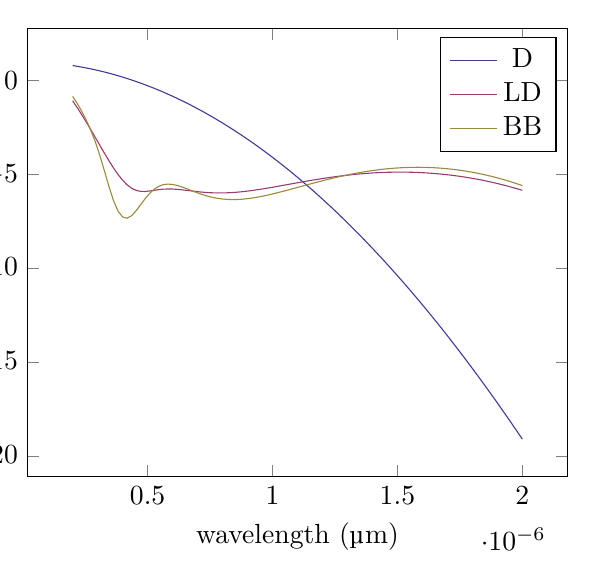
\begin{tikzpicture}[baseline,trim axis left]
\begin{axis}[xlabel=wavelength (\si{\micro\meter}),ylabel=$\epsilon'$]
\addplot[color=colora] coordinates {
(2e-07, 0.795370546512)
(2.18181818182e-07, 0.75648213635)
(2.36363636364e-07, 0.714215058474)
(2.54545454545e-07, 0.668570045805)
(2.72727272727e-07, 0.619547889747)
(2.90909090909e-07, 0.567149440156)
(3.09090909091e-07, 0.511375605302)
(3.27272727273e-07, 0.452227351829)
(3.45454545455e-07, 0.389705704712)
(3.63636363636e-07, 0.323811747218)
(3.81818181818e-07, 0.254546620851)
(4e-07, 0.181911525309)
(4.18181818182e-07, 0.105907718431)
(4.36363636364e-07, 0.0265365161392)
(4.54545454545e-07, -0.0562007076137)
(4.72727272727e-07, -0.142302520907)
(4.90909090909e-07, -0.231767433911)
(5.09090909091e-07, -0.324593898955)
(5.27272727273e-07, -0.420780310591)
(5.45454545455e-07, -0.520325005663)
(5.63636363636e-07, -0.623226263383)
(5.81818181818e-07, -0.729482305399)
(6e-07, -0.839091295877)
(6.18181818182e-07, -0.952051341576)
(6.36363636364e-07, -1.06836049193)
(6.54545454545e-07, -1.18801673915)
(6.72727272727e-07, -1.31101801826)
(6.90909090909e-07, -1.43736220725)
(7.09090909091e-07, -1.56704712714)
(7.27272727273e-07, -1.70007054203)
(7.45454545455e-07, -1.83643015929)
(7.63636363636e-07, -1.97612362957)
(7.81818181818e-07, -2.11914854696)
(8e-07, -2.26550244903)
(8.18181818182e-07, -2.41518281703)
(8.36363636364e-07, -2.5681870759)
(8.54545454545e-07, -2.72451259444)
(8.72727272727e-07, -2.88415668541)
(8.90909090909e-07, -3.04711660564)
(9.09090909091e-07, -3.21338955613)
(9.27272727273e-07, -3.38297268221)
(9.45454545455e-07, -3.55586307364)
(9.63636363636e-07, -3.73205776471)
(9.81818181818e-07, -3.91155373443)
(1e-06, -4.09434790658)
(1.01818181818e-06, -4.2804371499)
(1.03636363636e-06, -4.46981827821)
(1.05454545455e-06, -4.66248805053)
(1.07272727273e-06, -4.85844317123)
(1.09090909091e-06, -5.05768029016)
(1.10909090909e-06, -5.26019600281)
(1.12727272727e-06, -5.46598685044)
(1.14545454545e-06, -5.67504932024)
(1.16363636364e-06, -5.88737984545)
(1.18181818182e-06, -6.10297480554)
(1.2e-06, -6.32183052636)
(1.21818181818e-06, -6.54394328029)
(1.23636363636e-06, -6.76930928637)
(1.25454545455e-06, -6.99792471053)
(1.27272727273e-06, -7.22978566566)
(1.29090909091e-06, -7.46488821186)
(1.30909090909e-06, -7.70322835655)
(1.32727272727e-06, -7.94480205464)
(1.34545454545e-06, -8.18960520875)
(1.36363636364e-06, -8.43763366932)
(1.38181818182e-06, -8.68888323482)
(1.4e-06, -8.9433496519)
(1.41818181818e-06, -9.20102861562)
(1.43636363636e-06, -9.46191576956)
(1.45454545455e-06, -9.72600670605)
(1.47272727273e-06, -9.99329696635)
(1.49090909091e-06, -10.2637820408)
(1.50909090909e-06, -10.5374573691)
(1.52727272727e-06, -10.8143183403)
(1.54545454545e-06, -11.0943602933)
(1.56363636364e-06, -11.3775785167)
(1.58181818182e-06, -11.6639682493)
(1.6e-06, -11.95352468)
(1.61818181818e-06, -12.2462429484)
(1.63636363636e-06, -12.5421181446)
(1.65454545455e-06, -12.8411453096)
(1.67272727273e-06, -13.1433194354)
(1.69090909091e-06, -13.4486354653)
(1.70909090909e-06, -13.7570882942)
(1.72727272727e-06, -14.0686727686)
(1.74545454545e-06, -14.3833836869)
(1.76363636364e-06, -14.7012157997)
(1.78181818182e-06, -15.0221638097)
(1.8e-06, -15.3462223725)
(1.81818181818e-06, -15.6733860961)
(1.83636363636e-06, -16.0036495419)
(1.85454545455e-06, -16.337007224)
(1.87272727273e-06, -16.6734536104)
(1.89090909091e-06, -17.0129831226)
(1.90909090909e-06, -17.3555901358)
(1.92727272727e-06, -17.7012689795)
(1.94545454545e-06, -18.0500139376)
(1.96363636364e-06, -18.4018192484)
(1.98181818182e-06, -18.7566791051)
(2e-06, -19.1145876558)
};
\addlegendentry{D}
\addplot[color=colorb] coordinates {
(2e-07, -1.08159208556)
(2.18181818182e-07, -1.44171826843)
(2.36363636364e-07, -1.82088207661)
(2.54545454545e-07, -2.21603362179)
(2.72727272727e-07, -2.62365405323)
(2.90909090909e-07, -3.0395542098)
(3.09090909091e-07, -3.45859883423)
(3.27272727273e-07, -3.87436613042)
(3.45454545455e-07, -4.27879408412)
(3.63636363636e-07, -4.66194099615)
(3.81818181818e-07, -5.01209609134)
(4e-07, -5.31657282694)
(4.18181818182e-07, -5.56348358278)
(4.36363636364e-07, -5.74445904958)
(4.54545454545e-07, -5.85759179735)
(4.72727272727e-07, -5.90921039331)
(4.90909090909e-07, -5.91316759689)
(5.09090909091e-07, -5.88753097199)
(5.27272727273e-07, -5.85012422673)
(5.45454545455e-07, -5.81492603102)
(5.63636363636e-07, -5.7904975813)
(5.81818181818e-07, -5.78031080402)
(6e-07, -5.78411215554)
(6.18181818182e-07, -5.79947168917)
(6.36363636364e-07, -5.82303728722)
(6.54545454545e-07, -5.8513606632)
(6.72727272727e-07, -5.88135064692)
(6.90909090909e-07, -5.91046694848)
(7.09090909091e-07, -5.93675854119)
(7.27272727273e-07, -5.95882130326)
(7.45454545455e-07, -5.97572132891)
(7.63636363636e-07, -5.98690980118)
(7.81818181818e-07, -5.99214234135)
(8e-07, -5.99140827735)
(8.18181818182e-07, -5.98487130533)
(8.36363636364e-07, -5.97282109895)
(8.54545454545e-07, -5.95563462103)
(8.72727272727e-07, -5.933745667)
(8.90909090909e-07, -5.90762121552)
(9.09090909091e-07, -5.87774331799)
(9.27272727273e-07, -5.84459544679)
(9.45454545455e-07, -5.80865240418)
(9.63636363636e-07, -5.77037305563)
(9.81818181818e-07, -5.73019528891)
(1e-06, -5.68853271458)
(1.01818181818e-06, -5.64577271738)
(1.03636363636e-06, -5.60227554418)
(1.05454545455e-06, -5.55837417687)
(1.07272727273e-06, -5.51437478843)
(1.09090909091e-06, -5.47055762224)
(1.10909090909e-06, -5.4271781673)
(1.12727272727e-06, -5.38446852981)
(1.14545454545e-06, -5.34263892301)
(1.16363636364e-06, -5.30187921534)
(1.18181818182e-06, -5.26236049106)
(1.2e-06, -5.22423658926)
(1.21818181818e-06, -5.1876455963)
(1.23636363636e-06, -5.15271127402)
(1.25454545455e-06, -5.11954441204)
(1.27272727273e-06, -5.08824409678)
(1.29090909091e-06, -5.05889889355)
(1.30909090909e-06, -5.0315879406)
(1.32727272727e-06, -5.00638195606)
(1.34545454545e-06, -4.98334416022)
(1.36363636364e-06, -4.96253111645)
(1.38181818182e-06, -4.94399349513)
(1.4e-06, -4.92777676499)
(1.41818181818e-06, -4.91392181673)
(1.43636363636e-06, -4.90246552382)
(1.45454545455e-06, -4.89344124535)
(1.47272727273e-06, -4.88687927563)
(1.49090909091e-06, -4.88280724508)
(1.50909090909e-06, -4.88125047678)
(1.52727272727e-06, -4.88223230271)
(1.54545454545e-06, -4.88577434347)
(1.56363636364e-06, -4.89189675504)
(1.58181818182e-06, -4.90061844587)
(1.6e-06, -4.91195726727)
(1.61818181818e-06, -4.92593017979)
(1.63636363636e-06, -4.94255339827)
(1.65454545455e-06, -4.96184251765)
(1.67272727273e-06, -4.98381262178)
(1.69090909091e-06, -5.00847837698)
(1.70909090909e-06, -5.03585411214)
(1.72727272727e-06, -5.06595388683)
(1.74545454545e-06, -5.09879154883)
(1.76363636364e-06, -5.13438078228)
(1.78181818182e-06, -5.17273514763)
(1.8e-06, -5.2138681143)
(1.81818181818e-06, -5.25779308696)
(1.83636363636e-06, -5.30452342631)
(1.85454545455e-06, -5.35407246493)
(1.87272727273e-06, -5.40645351892)
(1.89090909091e-06, -5.46167989589)
(1.90909090909e-06, -5.51976489974)
(1.92727272727e-06, -5.58072183276)
(1.94545454545e-06, -5.64456399537)
(1.96363636364e-06, -5.7113046839)
(1.98181818182e-06, -5.78095718663)
(2e-06, -5.8535347785)
};
\addlegendentry{LD}
\addplot[color=colorc] coordinates {
(2e-07, -0.847496878826)
(2.18181818182e-07, -1.22118385656)
(2.36363636364e-07, -1.63991061742)
(2.54545454545e-07, -2.11139226584)
(2.72727272727e-07, -2.64918551278)
(2.90909090909e-07, -3.27391141233)
(3.09090909091e-07, -4.00198996909)
(3.27272727273e-07, -4.81803007312)
(3.45454545455e-07, -5.65403343443)
(3.63636363636e-07, -6.40313373125)
(3.81818181818e-07, -6.96248773068)
(4e-07, -7.27366299019)
(4.18181818182e-07, -7.33701540138)
(4.36363636364e-07, -7.20003316534)
(4.54545454545e-07, -6.93355195291)
(4.72727272727e-07, -6.6094007178)
(4.90909090909e-07, -6.28617926312)
(5.09090909091e-07, -6.00368458599)
(5.27272727273e-07, -5.78346940137)
(5.45454545455e-07, -5.63253472203)
(5.63636363636e-07, -5.54789298874)
(5.81818181818e-07, -5.52070947017)
(6e-07, -5.53949376625)
(6.18181818182e-07, -5.59227616137)
(6.36363636364e-07, -5.66792302087)
(6.54545454545e-07, -5.75681207713)
(6.72727272727e-07, -5.85107684358)
(6.90909090909e-07, -5.94458732949)
(7.09090909091e-07, -6.03278734318)
(7.27272727273e-07, -6.11246820204)
(7.45454545455e-07, -6.18152789563)
(7.63636363636e-07, -6.23874322011)
(7.81818181818e-07, -6.28356830772)
(8e-07, -6.31596431214)
(8.18181818182e-07, -6.33626005914)
(8.36363636364e-07, -6.34503978541)
(8.54545454545e-07, -6.34306072697)
(8.72727272727e-07, -6.3311807543)
(8.90909090909e-07, -6.31031225959)
(9.09090909091e-07, -6.28138473996)
(9.27272727273e-07, -6.24531863939)
(9.45454545455e-07, -6.20300674004)
(9.63636363636e-07, -6.15530250945)
(9.81818181818e-07, -6.10301215249)
(1e-06, -6.04689048476)
(1.01818181818e-06, -5.98763918946)
(1.03636363636e-06, -5.92590683842)
(1.05454545455e-06, -5.86229028132)
(1.07272727273e-06, -5.79733616152)
(1.09090909091e-06, -5.7315443446)
(1.10909090909e-06, -5.66537026386)
(1.12727272727e-06, -5.59922809558)
(1.14545454545e-06, -5.53349382212)
(1.16363636364e-06, -5.46850823988)
(1.18181818182e-06, -5.40457985805)
(1.2e-06, -5.34198765325)
(1.21818181818e-06, -5.2809836593)
(1.23636363636e-06, -5.22179538202)
(1.25454545455e-06, -5.16462803596)
(1.27272727273e-06, -5.10966660541)
(1.29090909091e-06, -5.05707773531)
(1.30909090909e-06, -5.00701146026)
(1.32727272727e-06, -4.95960278093)
(1.34545454545e-06, -4.914973098)
(1.36363636364e-06, -4.87323151418)
(1.38181818182e-06, -4.83447601445)
(1.4e-06, -4.79879453465)
(1.41818181818e-06, -4.76626592797)
(1.43636363636e-06, -4.73696083842)
(1.45454545455e-06, -4.71094248963)
(1.47272727273e-06, -4.68826739698)
(1.49090909091e-06, -4.66898601004)
(1.50909090909e-06, -4.65314329226)
(1.52727272727e-06, -4.64077924371)
(1.54545454545e-06, -4.63192937259)
(1.56363636364e-06, -4.62662512037)
(1.58181818182e-06, -4.62489424529)
(1.6e-06, -4.62676116823)
(1.61818181818e-06, -4.63224728466)
(1.63636363636e-06, -4.6413712462)
(1.65454545455e-06, -4.65414921462)
(1.67272727273e-06, -4.67059509115)
(1.69090909091e-06, -4.69072072357)
(1.70909090909e-06, -4.71453609325)
(1.72727272727e-06, -4.7420494841)
(1.74545454545e-06, -4.77326763533)
(1.76363636364e-06, -4.80819587962)
(1.78181818182e-06, -4.84683826804)
(1.8e-06, -4.88919768317)
(1.81818181818e-06, -4.93527594149)
(1.83636363636e-06, -4.98507388618)
(1.85454545455e-06, -5.03859147118)
(1.87272727273e-06, -5.09582783748)
(1.89090909091e-06, -5.15678138233)
(1.90909090909e-06, -5.22144982204)
(1.92727272727e-06, -5.28983024908)
(1.94545454545e-06, -5.36191918397)
(1.96363636364e-06, -5.43771262246)
(1.98181818182e-06, -5.51720607852)
(2e-06, -5.60039462344)
};
\addlegendentry{BB}
\end{axis}
\end{tikzpicture}%
\\
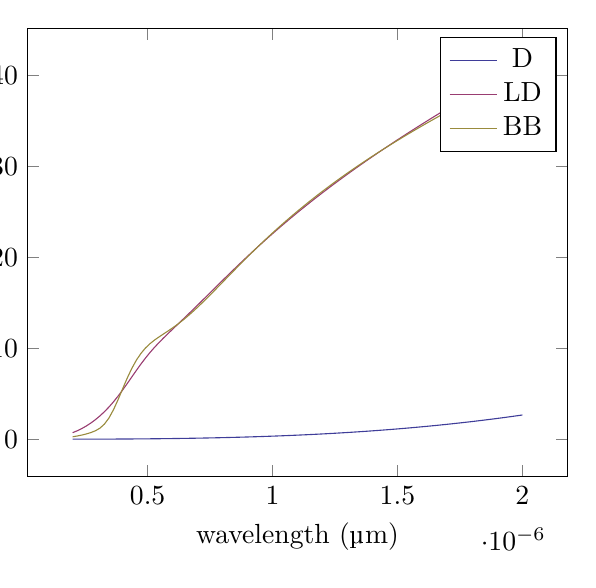
\begin{tikzpicture}[baseline,trim axis left]
\begin{axis}[xlabel=wavelength (\si{\micro\meter}),ylabel=$\epsilon''$]
\addplot[color=colora] coordinates {
(2e-07, 0.00270673459106)
(2.18181818182e-07, 0.00351396081869)
(2.36363636364e-07, 0.00446753061442)
(2.54545454545e-07, 0.00557962017657)
(2.72727272727e-07, 0.00686240112315)
(2.90909090909e-07, 0.00832804014095)
(3.09090909091e-07, 0.00998869863483)
(3.27272727273e-07, 0.0118565323774)
(3.45454545455e-07, 0.0139436911588)
(3.63636363636e-07, 0.0162623184375)
(3.81818181818e-07, 0.0188245509904)
(4e-07, 0.0216425185646)
(4.18181818182e-07, 0.0247283435284)
(4.36363636364e-07, 0.0280941405237)
(4.54545454545e-07, 0.0317520161183)
(4.72727272727e-07, 0.0357140684589)
(4.90909090909e-07, 0.0399923869245)
(5.09090909091e-07, 0.0445990517805)
(5.27272727273e-07, 0.0495461338331)
(5.45454545455e-07, 0.0548456940848)
(5.63636363636e-07, 0.0605097833895)
(5.81818181818e-07, 0.0665504421093)
(6e-07, 0.0729796997715)
(6.18181818182e-07, 0.0798095747257)
(6.36363636364e-07, 0.0870520738028)
(6.54545454545e-07, 0.0947191919732)
(6.72727272727e-07, 0.102822912007)
(6.90909090909e-07, 0.111375204135)
(7.09090909091e-07, 0.120388025708)
(7.27272727273e-07, 0.129873320861)
(7.45454545455e-07, 0.139843020175)
(7.63636363636e-07, 0.150309040339)
(7.81818181818e-07, 0.161283283817)
(8e-07, 0.172777638513)
(8.18181818182e-07, 0.184803977434)
(8.36363636364e-07, 0.197374158362)
(8.54545454545e-07, 0.210500023517)
(8.72727272727e-07, 0.224193399229)
(8.90909090909e-07, 0.238466095607)
(9.09090909091e-07, 0.253329906209)
(9.27272727273e-07, 0.268796607716)
(9.45454545455e-07, 0.284877959601)
(9.63636363636e-07, 0.301585703806)
(9.81818181818e-07, 0.318931564417)
(1e-06, 0.336927247338)
(1.01818181818e-06, 0.355584439967)
(1.03636363636e-06, 0.374914810879)
(1.05454545455e-06, 0.394930009501)
(1.07272727273e-06, 0.415641665791)
(1.09090909091e-06, 0.437061389926)
(1.10909090909e-06, 0.459200771978)
(1.12727272727e-06, 0.4820713816)
(1.14545454545e-06, 0.505684767714)
(1.16363636364e-06, 0.530052458193)
(1.18181818182e-06, 0.555185959551)
(1.2e-06, 0.581096756631)
(1.21818181818e-06, 0.607796312296)
(1.23636363636e-06, 0.635296067118)
(1.25454545455e-06, 0.663607439074)
(1.27272727273e-06, 0.692741823238)
(1.29090909091e-06, 0.722710591477)
(1.30909090909e-06, 0.753525092145)
(1.32727272727e-06, 0.785196649788)
(1.34545454545e-06, 0.817736564834)
(1.36363636364e-06, 0.851156113304)
(1.38181818182e-06, 0.885466546505)
(1.4e-06, 0.920679090741)
(1.41818181818e-06, 0.956804947013)
(1.43636363636e-06, 0.993855290729)
(1.45454545455e-06, 1.03184127141)
(1.47272727273e-06, 1.07077401241)
(1.49090909091e-06, 1.1106646106)
(1.50909090909e-06, 1.15152413611)
(1.52727272727e-06, 1.19336363204)
(1.54545454545e-06, 1.23619411414)
(1.56363636364e-06, 1.2800265706)
(1.58181818182e-06, 1.32487196168)
(1.6e-06, 1.3707412195)
(1.61818181818e-06, 1.41764524773)
(1.63636363636e-06, 1.46559492132)
(1.65454545455e-06, 1.51460108624)
(1.67272727273e-06, 1.56467455917)
(1.69090909091e-06, 1.61582612726)
(1.70909090909e-06, 1.66806654788)
(1.72727272727e-06, 1.72140654829)
(1.74545454545e-06, 1.77585682543)
(1.76363636364e-06, 1.83142804563)
(1.78181818182e-06, 1.88813084435)
(1.8e-06, 1.94597582592)
(1.81818181818e-06, 2.00497356328)
(1.83636363636e-06, 2.06513459776)
(1.85454545455e-06, 2.12646943873)
(1.87272727273e-06, 2.18898856346)
(1.89090909091e-06, 2.25270241679)
(1.90909090909e-06, 2.31762141091)
(1.92727272727e-06, 2.38375592509)
(1.94545454545e-06, 2.45111630548)
(1.96363636364e-06, 2.51971286481)
(1.98181818182e-06, 2.58955588219)
(2e-06, 2.66065560284)
};
\addlegendentry{D}
\addplot[color=colorb] coordinates {
(2e-07, 0.717563282282)
(2.18181818182e-07, 0.925670770217)
(2.36363636364e-07, 1.16954998857)
(2.54545454545e-07, 1.45196388618)
(2.72727272727e-07, 1.77578802193)
(2.90909090909e-07, 2.14400598293)
(3.09090909091e-07, 2.55962385163)
(3.27272727273e-07, 3.02543842534)
(3.45454545455e-07, 3.54357205439)
(3.63636363636e-07, 4.11468514783)
(3.81818181818e-07, 4.73683482871)
(4e-07, 5.40411868846)
(4.18181818182e-07, 6.10554809283)
(4.36363636364e-07, 6.82492206272)
(4.54545454545e-07, 7.54248909632)
(4.72727272727e-07, 8.23851777226)
(4.90909090909e-07, 8.89767090463)
(5.09090909091e-07, 9.51222412362)
(5.27272727273e-07, 10.0826520321)
(5.45454545455e-07, 10.6156615301)
(5.63636363636e-07, 11.1210371984)
(5.81818181818e-07, 11.6087866305)
(6e-07, 12.0873576171)
(6.18181818182e-07, 12.5629441178)
(6.36363636364e-07, 13.0395269845)
(6.54545454545e-07, 13.5192673102)
(6.72727272727e-07, 14.0029896553)
(6.90909090909e-07, 14.490620533)
(7.09090909091e-07, 14.9815343767)
(7.27272727273e-07, 15.4748044682)
(7.45454545455e-07, 15.969374309)
(7.63636363636e-07, 16.4641687747)
(7.81818181818e-07, 16.958162337)
(8e-07, 17.4504178793)
(8.18181818182e-07, 17.9401059821)
(8.36363636364e-07, 18.4265115988)
(8.54545454545e-07, 18.9090328441)
(8.72727272727e-07, 19.3871750659)
(8.90909090909e-07, 19.860542293)
(9.09090909091e-07, 20.3288274283)
(9.27272727273e-07, 20.7918020645)
(9.45454545455e-07, 21.2493064758)
(9.63636363636e-07, 21.7012401179)
(9.81818181818e-07, 22.1475528265)
(1e-06, 22.5882368075)
(1.01818181818e-06, 23.0233194502)
(1.03636363636e-06, 23.4528569521)
(1.05454545455e-06, 23.8769287225)
(1.07272727273e-06, 24.2956325125)
(1.09090909091e-06, 24.7090802137)
(1.10909090909e-06, 25.1173942632)
(1.12727272727e-06, 25.5207045937)
(1.14545454545e-06, 25.9191460666)
(1.16363636364e-06, 26.3128563325)
(1.18181818182e-06, 26.7019740653)
(1.2e-06, 27.0866375206)
(1.21818181818e-06, 27.4669833755)
(1.23636363636e-06, 27.8431458089)
(1.25454545455e-06, 28.2152557871)
(1.27272727273e-06, 28.5834405237)
(1.29090909091e-06, 28.9478230868)
(1.30909090909e-06, 29.3085221276)
(1.32727272727e-06, 29.6656517124)
(1.34545454545e-06, 30.0193212369)
(1.36363636364e-06, 30.3696354097)
(1.38181818182e-06, 30.7166942906)
(1.4e-06, 31.0605933723)
(1.41818181818e-06, 31.4014236969)
(1.43636363636e-06, 31.7392719979)
(1.45454545455e-06, 32.0742208616)
(1.47272727273e-06, 32.4063489033)
(1.49090909091e-06, 32.7357309506)
(1.50909090909e-06, 33.0624382343)
(1.52727272727e-06, 33.3865385795)
(1.54545454545e-06, 33.7080965977)
(1.56363636364e-06, 34.0271738756)
(1.58181818182e-06, 34.3438291607)
(1.6e-06, 34.6581185415)
(1.61818181818e-06, 34.9700956215)
(1.63636363636e-06, 35.2798116867)
(1.65454545455e-06, 35.5873158658)
(1.67272727273e-06, 35.8926552831)
(1.69090909091e-06, 36.1958752037)
(1.70909090909e-06, 36.4970191711)
(1.72727272727e-06, 36.7961291371)
(1.74545454545e-06, 37.0932455844)
(1.76363636364e-06, 37.3884076415)
(1.78181818182e-06, 37.6816531913)
(1.8e-06, 37.973018972)
(1.81818181818e-06, 38.2625406722)
(1.83636363636e-06, 38.5502530186)
(1.85454545455e-06, 38.8361898592)
(1.87272727273e-06, 39.1203842397)
(1.89090909091e-06, 39.4028684745)
(1.90909090909e-06, 39.6836742134)
(1.92727272727e-06, 39.9628325027)
(1.94545454545e-06, 40.2403738417)
(1.96363636364e-06, 40.5163282358)
(1.98181818182e-06, 40.7907252444)
(2e-06, 41.0635940258)
};
\addlegendentry{LD}
\addplot[color=colorc] coordinates {
(2e-07, 0.268842660424)
(2.18181818182e-07, 0.352903437773)
(2.36363636364e-07, 0.454584963212)
(2.54545454545e-07, 0.577109140464)
(2.72727272727e-07, 0.727270632599)
(2.90909090909e-07, 0.924365322096)
(3.09090909091e-07, 1.21337770529)
(3.27272727273e-07, 1.66357011238)
(3.45454545455e-07, 2.33747647917)
(3.63636363636e-07, 3.24917964361)
(3.81818181818e-07, 4.34702562775)
(4e-07, 5.53250298964)
(4.18181818182e-07, 6.69771157435)
(4.36363636364e-07, 7.7575893669)
(4.54545454545e-07, 8.66490161621)
(4.72727272727e-07, 9.40912441366)
(4.90909090909e-07, 10.0063699431)
(5.09090909091e-07, 10.487244061)
(5.27272727273e-07, 10.8867311824)
(5.45454545455e-07, 11.237519712)
(5.63636363636e-07, 11.5665515447)
(5.81818181818e-07, 11.8939265879)
(6e-07, 12.2332350121)
(6.18181818182e-07, 12.592587104)
(6.36363636364e-07, 12.9758593713)
(6.54545454545e-07, 13.3838851006)
(6.72727272727e-07, 13.8154637847)
(6.90909090909e-07, 14.2681529254)
(7.09090909091e-07, 14.7388531113)
(7.27272727273e-07, 15.2242179794)
(7.45454545455e-07, 15.7209260965)
(7.63636363636e-07, 16.2258494974)
(7.81818181818e-07, 16.7361481378)
(8e-07, 17.249313328)
(8.18181818182e-07, 17.7631775034)
(8.36363636364e-07, 18.2759018151)
(8.54545454545e-07, 18.7859572903)
(8.72727272727e-07, 19.2920876864)
(8.90909090909e-07, 19.793282612)
(9.09090909091e-07, 20.2887444701)
(9.27272727273e-07, 20.7778584407)
(9.45454545455e-07, 21.260164979)
(9.63636363636e-07, 21.735335218)
(9.81818181818e-07, 22.2031492894)
(1e-06, 22.6634774908)
(1.01818181818e-06, 23.1162640813)
(1.03636363636e-06, 23.5615134544)
(1.05454545455e-06, 23.9992784595)
(1.07272727273e-06, 24.4296503811)
(1.09090909091e-06, 24.8527509001)
(1.10909090909e-06, 25.2687250513)
(1.12727272727e-06, 25.677735544)
(1.14545454545e-06, 26.0799580435)
(1.16363636364e-06, 26.4755772935)
(1.18181818182e-06, 26.8647839491)
(1.2e-06, 27.2477720037)
(1.21818181818e-06, 27.6247367143)
(1.23636363636e-06, 27.9958729403)
(1.25454545455e-06, 28.3613738285)
(1.27272727273e-06, 28.7214297824)
(1.29090909091e-06, 29.0762276688)
(1.30909090909e-06, 29.4259502176)
(1.32727272727e-06, 29.7707755824)
(1.34545454545e-06, 30.1108770308)
(1.36363636364e-06, 30.4464227408)
(1.38181818182e-06, 30.7775756835)
(1.4e-06, 31.1044935746)
(1.41818181818e-06, 31.4273288806)
(1.43636363636e-06, 31.7462288692)
(1.45454545455e-06, 32.0613356932)
(1.47272727273e-06, 32.3727865003)
(1.49090909091e-06, 32.6807135628)
(1.50909090909e-06, 32.9852444216)
(1.52727272727e-06, 33.2865020399)
(1.54545454545e-06, 33.5846049631)
(1.56363636364e-06, 33.8796674834)
(1.58181818182e-06, 34.1717998041)
(1.6e-06, 34.4611082051)
(1.61818181818e-06, 34.7476952047)
(1.63636363636e-06, 35.0316597203)
(1.65454545455e-06, 35.3130972236)
(1.67272727273e-06, 35.5920998921)
(1.69090909091e-06, 35.8687567557)
(1.70909090909e-06, 36.1431538375)
(1.72727272727e-06, 36.4153742898)
(1.74545454545e-06, 36.6854985237)
(1.76363636364e-06, 36.9536043343)
(1.78181818182e-06, 37.219767019)
(1.8e-06, 37.4840594913)
(1.81818181818e-06, 37.7465523888)
(1.83636363636e-06, 38.0073141763)
(1.85454545455e-06, 38.2664112431)
(1.87272727273e-06, 38.5239079967)
(1.89090909091e-06, 38.7798669505)
(1.90909090909e-06, 39.0343488077)
(1.92727272727e-06, 39.2874125411)
(1.94545454545e-06, 39.5391154681)
(1.96363636364e-06, 39.7895133223)
(1.98181818182e-06, 40.0386603216)
(2e-06, 40.2866092318)
};
\addlegendentry{BB}
\end{axis}
\end{tikzpicture}%
\\
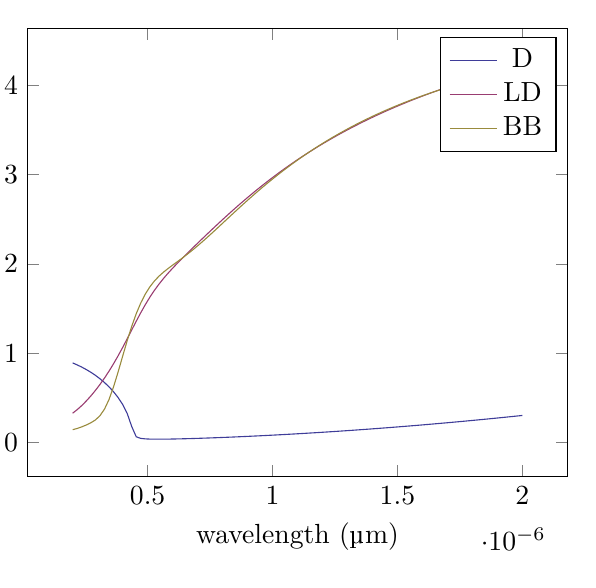
\begin{tikzpicture}[baseline,trim axis left]
\begin{axis}[xlabel=wavelength (\si{\micro\meter}),ylabel=$n'$]
\addplot[color=colora] coordinates {
(2e-07, 0.891836784022)
(2.18181818182e-07, 0.869762161187)
(2.36363636364e-07, 0.845116586447)
(2.54545454545e-07, 0.817668445598)
(2.72727272727e-07, 0.787125715469)
(2.90909090909e-07, 0.753113544433)
(3.09090909091e-07, 0.715139411554)
(3.27272727273e-07, 0.672536283299)
(3.45454545455e-07, 0.624363989452)
(3.63636363636e-07, 0.569223855988)
(3.81818181818e-07, 0.50487045912)
(4e-07, 0.427262192361)
(4.18181818182e-07, 0.327615653057)
(4.36363636364e-07, 0.180529668395)
(4.54545454545e-07, 0.0646117287163)
(4.72727272727e-07, 0.0469744499216)
(4.90909090909e-07, 0.0413830500412)
(5.09090909091e-07, 0.0390488072526)
(5.27272727273e-07, 0.0381244236549)
(5.45454545455e-07, 0.0379642245608)
(5.63636363636e-07, 0.0382791938781)
(5.81818181818e-07, 0.0389191324397)
(6e-07, 0.0397976997315)
(6.18181818182e-07, 0.0408615020759)
(6.36363636364e-07, 0.0420756354457)
(6.54545454545e-07, 0.0434162634968)
(6.72727272727e-07, 0.0448665225187)
(6.90909090909e-07, 0.0464141281504)
(7.09090909091e-07, 0.0480499092258)
(7.27272727273e-07, 0.0497668736032)
(7.45454545455e-07, 0.0515595927984)
(7.63636363636e-07, 0.0534237848634)
(7.81818181818e-07, 0.055356024533)
(8e-07, 0.0573535373724)
(8.18181818182e-07, 0.0594140507382)
(8.36363636364e-07, 0.0615356840052)
(8.54545454545e-07, 0.0637168664607)
(8.72727272727e-07, 0.0659562750339)
(8.90909090909e-07, 0.0682527864717)
(9.09090909091e-07, 0.070605440186)
(9.27272727273e-07, 0.0730134090869)
(9.45454545455e-07, 0.0754759764641)
(9.63636363636e-07, 0.0779925174999)
(9.81818181818e-07, 0.0805624843626)
(1e-06, 0.0831853940971)
(1.01818181818e-06, 0.0858608187167)
(1.03636363636e-06, 0.0885883770432)
(1.05454545455e-06, 0.0913677279445)
(1.07272727273e-06, 0.0941985646997)
(1.09090909091e-06, 0.0970806102759)
(1.10909090909e-06, 0.100013613351)
(1.12727272727e-06, 0.102997344947)
(1.14545454545e-06, 0.10603159557)
(1.16363636364e-06, 0.109116172765)
(1.18181818182e-06, 0.112250899024)
(1.2e-06, 0.115435609983)
(1.21818181818e-06, 0.118670152864)
(1.23636363636e-06, 0.121954385131)
(1.25454545455e-06, 0.125288173312)
(1.27272727273e-06, 0.128671391982)
(1.29090909091e-06, 0.132103922861)
(1.30909090909e-06, 0.135585654039)
(1.32727272727e-06, 0.139116479275)
(1.34545454545e-06, 0.142696297398)
(1.36363636364e-06, 0.14632501176)
(1.38181818182e-06, 0.150002529766)
(1.4e-06, 0.153728762447)
(1.41818181818e-06, 0.157503624081)
(1.43636363636e-06, 0.161327031862)
(1.45454545455e-06, 0.165198905593)
(1.47272727273e-06, 0.169119167421)
(1.49090909091e-06, 0.173087741593)
(1.50909090909e-06, 0.177104554242)
(1.52727272727e-06, 0.181169533186)
(1.54545454545e-06, 0.185282607757)
(1.56363636364e-06, 0.189443708638)
(1.58181818182e-06, 0.193652767722)
(1.6e-06, 0.197909717979)
(1.61818181818e-06, 0.202214493338)
(1.63636363636e-06, 0.206567028582)
(1.65454545455e-06, 0.210967259244)
(1.67272727273e-06, 0.215415121527)
(1.69090909091e-06, 0.219910552213)
(1.70909090909e-06, 0.224453488598)
(1.72727272727e-06, 0.229043868417)
(1.74545454545e-06, 0.233681629785)
(1.76363636364e-06, 0.238366711142)
(1.78181818182e-06, 0.243099051198)
(1.8e-06, 0.247878588886)
(1.81818181818e-06, 0.252705263319)
(1.83636363636e-06, 0.257579013751)
(1.85454545455e-06, 0.262499779536)
(1.87272727273e-06, 0.2674675001)
(1.89090909091e-06, 0.272482114902)
(1.90909090909e-06, 0.277543563414)
(1.92727272727e-06, 0.282651785086)
(1.94545454545e-06, 0.287806719327)
(1.96363636364e-06, 0.29300830548)
(1.98181818182e-06, 0.298256482802)
(2e-06, 0.303551190446)
};
\addlegendentry{D}
\addplot[color=colorb] coordinates {
(2e-07, 0.328924523612)
(2.18181818182e-07, 0.368502289531)
(2.36363636364e-07, 0.414275232349)
(2.54545454545e-07, 0.465460363411)
(2.72727272727e-07, 0.521759448907)
(2.90909090909e-07, 0.583127920347)
(3.09090909091e-07, 0.649669981986)
(3.27272727273e-07, 0.72156845815)
(3.45454545455e-07, 0.799009401671)
(3.63636363636e-07, 0.882078123467)
(3.81818181818e-07, 0.970614842165)
(4e-07, 1.0640379682)
(4.18181818182e-07, 1.16117736704)
(4.36363636364e-07, 1.26020076609)
(4.54545454545e-07, 1.35873189351)
(4.72727272727e-07, 1.45420523581)
(4.90909090909e-07, 1.54437504346)
(5.09090909091e-07, 1.62777621238)
(5.27272727273e-07, 1.70393626008)
(5.45454545455e-07, 1.77327735583)
(5.63636363636e-07, 1.83680934873)
(5.81818181818e-07, 1.89577887415)
(6e-07, 1.95139617938)
(6.18181818182e-07, 2.00468044811)
(6.36363636364e-07, 2.05640644229)
(6.54545454545e-07, 2.10711473619)
(6.72727272727e-07, 2.15715150869)
(6.90909090909e-07, 2.20671566984)
(7.09090909091e-07, 2.25590194139)
(7.27272727273e-07, 2.30473565908)
(7.45454545455e-07, 2.3531988687)
(7.63636363636e-07, 2.40124890738)
(7.81818181818e-07, 2.44883110046)
(8e-07, 2.49588710944)
(8.18181818182e-07, 2.54236018735)
(8.36363636364e-07, 2.58819829595)
(8.54545454545e-07, 2.63335577951)
(8.72727272727e-07, 2.67779408652)
(8.90909090909e-07, 2.72148188009)
(9.09090909091e-07, 2.76439477025)
(9.27272727273e-07, 2.80651482538)
(9.45454545455e-07, 2.84782996752)
(9.63636363636e-07, 2.88833332048)
(9.81818181818e-07, 2.92802255479)
(1e-06, 2.96689925703)
(1.01818181818e-06, 3.00496833963)
(1.03636363636e-06, 3.04223749985)
(1.05454545455e-06, 3.07871673154)
(1.07272727273e-06, 3.11441788997)
(1.09090909091e-06, 3.14935430819)
(1.10909090909e-06, 3.18354046184)
(1.12727272727e-06, 3.21699167881)
(1.14545454545e-06, 3.24972388978)
(1.16363636364e-06, 3.28175341565)
(1.18181818182e-06, 3.31309678785)
(1.2e-06, 3.34377059777)
(1.21818181818e-06, 3.37379137185)
(1.23636363636e-06, 3.40317546906)
(1.25454545455e-06, 3.43193899784)
(1.27272727273e-06, 3.4600977499)
(1.29090909091e-06, 3.48766714842)
(1.30909090909e-06, 3.51466220865)
(1.32727272727e-06, 3.54109750897)
(1.34545454545e-06, 3.56698717088)
(1.36363636364e-06, 3.5923448464)
(1.38181818182e-06, 3.61718371169)
(1.4e-06, 3.64151646582)
(1.41818181818e-06, 3.66535533372)
(1.43636363636e-06, 3.68871207265)
(1.45454545455e-06, 3.71159798124)
(1.47272727273e-06, 3.73402391085)
(1.49090909091e-06, 3.75600027847)
(1.50909090909e-06, 3.77753708094)
(1.52727272727e-06, 3.79864391006)
(1.54545454545e-06, 3.81932996823)
(1.56363636364e-06, 3.83960408456)
(1.58181818182e-06, 3.85947473103)
(1.6e-06, 3.87895003871)
(1.61818181818e-06, 3.89803781383)
(1.63636363636e-06, 3.91674555353)
(1.65454545455e-06, 3.93508046143)
(1.67272727273e-06, 3.95304946258)
(1.69090909091e-06, 3.97065921818)
(1.70909090909e-06, 3.98791613965)
(1.72727272727e-06, 4.00482640228)
(1.74545454545e-06, 4.02139595829)
(1.76363636364e-06, 4.0376305494)
(1.78181818182e-06, 4.05353571881)
(1.8e-06, 4.0691168227)
(1.81818181818e-06, 4.08437904114)
(1.83636363636e-06, 4.0993273885)
(1.85454545455e-06, 4.11396672337)
(1.87272727273e-06, 4.12830175795)
(1.89090909091e-06, 4.14233706698)
(1.90909090909e-06, 4.15607709619)
(1.92727272727e-06, 4.16952617036)
(1.94545454545e-06, 4.18268850084)
(1.96363636364e-06, 4.19556819278)
(1.98181818182e-06, 4.20816925191)
(2e-06, 4.2204955909)
};
\addlegendentry{LD}
\addplot[color=colorc] coordinates {
(2e-07, 0.144255264924)
(2.18181818182e-07, 0.158065645953)
(2.36363636364e-07, 0.175840485401)
(2.54545454545e-07, 0.196787207606)
(2.72727272727e-07, 0.221375512414)
(2.90909090909e-07, 0.252974358945)
(3.09090909091e-07, 0.299917198736)
(3.27272727273e-07, 0.373573391157)
(3.45454545455e-07, 0.481729834547)
(3.63636363636e-07, 0.623380616283)
(3.81818181818e-07, 0.789179931972)
(4e-07, 0.965654749451)
(4.18181818182e-07, 1.13958891963)
(4.36363636364e-07, 1.30075912776)
(4.54545454545e-07, 1.44290593874)
(4.72727272727e-07, 1.56350763238)
(4.90909090909e-07, 1.66296502781)
(5.09090909091e-07, 1.74362533283)
(5.27272727273e-07, 1.80888348623)
(5.45454545455e-07, 1.86246618904)
(5.63636363636e-07, 1.90792637438)
(5.81818181818e-07, 1.94833542443)
(6e-07, 1.98614020477)
(6.18181818182e-07, 2.02314290371)
(6.36363636364e-07, 2.06056041216)
(6.54545454545e-07, 2.099124983)
(6.72727272727e-07, 2.13919697908)
(6.90909090909e-07, 2.18087082598)
(7.09090909091e-07, 2.2240644119)
(7.27272727273e-07, 2.26858884155)
(7.45454545455e-07, 2.31419949969)
(7.63636363636e-07, 2.36063132546)
(7.81818181818e-07, 2.40762175471)
(8e-07, 2.45492457791)
(8.18181818182e-07, 2.50231742224)
(8.36363636364e-07, 2.54960492816)
(8.54545454545e-07, 2.59661936906)
(8.72727272727e-07, 2.64321917826)
(8.90909090909e-07, 2.6892870947)
(9.09090909091e-07, 2.73472758243)
(9.27272727273e-07, 2.77946419803)
(9.45454545455e-07, 2.82343705623)
(9.63636363636e-07, 2.86660041663)
(9.81818181818e-07, 2.90892054998)
(1e-06, 2.95037382088)
(1.01818181818e-06, 2.99094501635)
(1.03636363636e-06, 3.0306259007)
(1.05454545455e-06, 3.06941397113)
(1.07272727273e-06, 3.10731142565)
(1.09090909091e-06, 3.14432423669)
(1.10909090909e-06, 3.18046142113)
(1.12727272727e-06, 3.21573440362)
(1.14545454545e-06, 3.25015648904)
(1.16363636364e-06, 3.28374242311)
(1.18181818182e-06, 3.31650802785)
(1.2e-06, 3.34846990015)
(1.21818181818e-06, 3.37964516363)
(1.23636363636e-06, 3.41005126525)
(1.25454545455e-06, 3.43970580942)
(1.27272727273e-06, 3.46862642361)
(1.29090909091e-06, 3.49683065015)
(1.30909090909e-06, 3.52433586005)
(1.32727272727e-06, 3.55115918494)
(1.34545454545e-06, 3.57731746424)
(1.36363636364e-06, 3.60282720492)
(1.38181818182e-06, 3.62770455153)
(1.4e-06, 3.65196526492)
(1.41818181818e-06, 3.6756247079)
(1.43636363636e-06, 3.69869783671)
(1.45454545455e-06, 3.7211991971)
(1.47272727273e-06, 3.74314292426)
(1.49090909091e-06, 3.76454274575)
(1.50909090909e-06, 3.78541198683)
(1.52727272727e-06, 3.80576357771)
(1.54545454545e-06, 3.82561006227)
(1.56363636364e-06, 3.84496360785)
(1.58181818182e-06, 3.86383601588)
(1.6e-06, 3.88223873306)
(1.61818181818e-06, 3.90018286294)
(1.63636363636e-06, 3.91767917765)
(1.65454545455e-06, 3.93473812976)
(1.67272727273e-06, 3.95136986409)
(1.69090909091e-06, 3.96758422934)
(1.70909090909e-06, 3.98339078963)
(1.72727272727e-06, 3.99879883571)
(1.74545454545e-06, 4.01381739596)
(1.76363636364e-06, 4.02845524701)
(1.78181818182e-06, 4.04272092405)
(1.8e-06, 4.05662273082)
(1.81818181818e-06, 4.07016874918)
(1.83636363636e-06, 4.08336684836)
(1.85454545455e-06, 4.09622469382)
(1.87272727273e-06, 4.10874975575)
(1.89090909091e-06, 4.1209493172)
(1.90909090909e-06, 4.13283048189)
(1.92727272727e-06, 4.14440018162)
(1.94545454545e-06, 4.1556651834)
(1.96363636364e-06, 4.1666320962)
(1.98181818182e-06, 4.17730737739)
(2e-06, 4.18769733896)
};
\addlegendentry{BB}
\end{axis}
\end{tikzpicture}%
\\
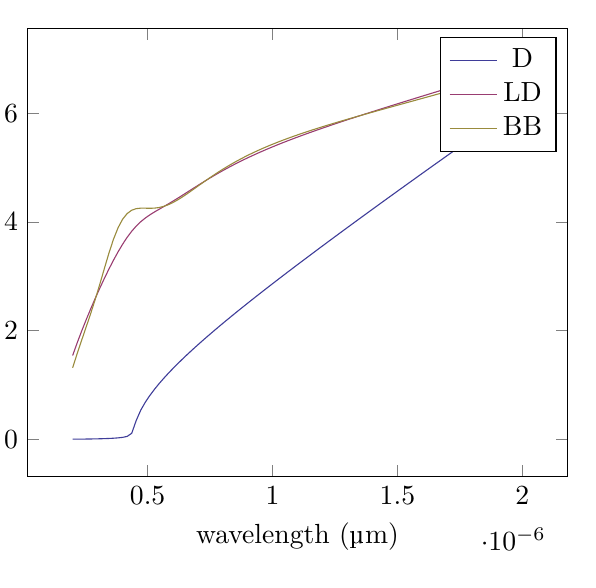
\begin{tikzpicture}[baseline,trim axis left]
\begin{axis}[xlabel=wavelength (\si{\micro\meter}),ylabel=$n''$]
\addplot[color=colora] coordinates {
(2e-07, 0.00214607697114)
(2.18181818182e-07, 0.00285681032654)
(2.36363636364e-07, 0.00373797088269)
(2.54545454545e-07, 0.00482516756583)
(2.72727272727e-07, 0.00616477174362)
(2.90909090909e-07, 0.00781929059859)
(3.09090909091e-07, 0.00987650299481)
(3.27272727273e-07, 0.0124659957441)
(3.45454545455e-07, 0.0157915554704)
(3.63636363636e-07, 0.0202015349919)
(3.81818181818e-07, 0.0263651148877)
(4e-07, 0.0358177529221)
(4.18181818182e-07, 0.0533722343034)
(4.36363636364e-07, 0.11004040196)
(4.54545454545e-07, 0.347492109555)
(4.72727272727e-07, 0.537604166376)
(4.90909090909e-07, 0.683344701804)
(5.09090909091e-07, 0.807612169674)
(5.27272727273e-07, 0.918949163196)
(5.45454545455e-07, 1.02153442234)
(5.63636363636e-07, 1.11775807764)
(5.81818181818e-07, 1.20912944242)
(6e-07, 1.29666892674)
(6.18181818182e-07, 1.38110173697)
(6.36363636364e-07, 1.46296332902)
(6.54545454545e-07, 1.5426611495)
(6.72727272727e-07, 1.62051289603)
(6.90909090909e-07, 1.69677133318)
(7.09090909091e-07, 1.77164100252)
(7.27272727273e-07, 1.84528983292)
(7.45454545455e-07, 1.91785742479)
(7.63636363636e-07, 1.98946109807)
(7.81818181818e-07, 2.06020039628)
(8e-07, 2.13016049972)
(8.18181818182e-07, 2.19941485239)
(8.36363636364e-07, 2.26802721161)
(8.54545454545e-07, 2.33605326716)
(8.72727272727e-07, 2.40354193457)
(8.90909090909e-07, 2.47053639864)
(9.09090909091e-07, 2.53707496315)
(9.27272727273e-07, 2.60319174865)
(9.45454545455e-07, 2.66891726985)
(9.63636363636e-07, 2.73427891683)
(9.81818181818e-07, 2.79930135867)
(1e-06, 2.8640068842)
(1.01818181818e-06, 2.92841569115)
(1.03636363636e-06, 2.9925461329)
(1.05454545455e-06, 3.05641493003)
(1.07272727273e-06, 3.1200373526)
(1.09090909091e-06, 3.18342737786)
(1.10909090909e-06, 3.24659782716)
(1.12727272727e-06, 3.30956048548)
(1.14545454545e-06, 3.3723262059)
(1.16363636364e-06, 3.43490500148)
(1.18181818182e-06, 3.49730612611)
(1.2e-06, 3.559538146)
(1.21818181818e-06, 3.62160900304)
(1.23636363636e-06, 3.68352607115)
(1.25454545455e-06, 3.74529620642)
(1.27272727273e-06, 3.80692579197)
(1.29090909091e-06, 3.86842077812)
(1.30909090909e-06, 3.92978671842)
(1.32727272727e-06, 3.99102880206)
(1.34545454545e-06, 4.05215188315)
(1.36363636364e-06, 4.11316050705)
(1.38181818182e-06, 4.17405893436)
(1.4e-06, 4.23485116251)
(1.41818181818e-06, 4.2955409455)
(1.43636363636e-06, 4.35613181177)
(1.45454545455e-06, 4.41662708058)
(1.47272727273e-06, 4.47702987686)
(1.49090909091e-06, 4.53734314486)
(1.50909090909e-06, 4.59756966064)
(1.52727272727e-06, 4.65771204349)
(1.54545454545e-06, 4.71777276647)
(1.56363636364e-06, 4.77775416601)
(1.58181818182e-06, 4.83765845088)
(1.6e-06, 4.89748771035)
(1.61818181818e-06, 4.95724392173)
(1.63636363636e-06, 5.01692895742)
(1.65454545455e-06, 5.07654459136)
(1.67272727273e-06, 5.136092505)
(1.69090909091e-06, 5.19557429285)
(1.70909090909e-06, 5.25499146769)
(1.72727272727e-06, 5.3143454653)
(1.74545454545e-06, 5.37363764894)
(1.76363636364e-06, 5.43286931348)
(1.78181818182e-06, 5.49204168929)
(1.8e-06, 5.5511559458)
(1.81818181818e-06, 5.61021319493)
(1.83636363636e-06, 5.66921449412)
(1.85454545455e-06, 5.7281608494)
(1.87272727273e-06, 5.78705321801)
(1.89090909091e-06, 5.84589251107)
(1.90909090909e-06, 5.90467959594)
(1.92727272727e-06, 5.96341529849)
(1.94545454545e-06, 6.02210040522)
(1.96363636364e-06, 6.08073566527)
(1.98181818182e-06, 6.13932179228)
(2e-06, 6.19785946615)
};
\addlegendentry{D}
\addplot[color=colorb] coordinates {
(2e-07, 1.54258447276)
(2.18181818182e-07, 1.77623883857)
(2.36363636364e-07, 1.99624950582)
(2.54545454545e-07, 2.20575926687)
(2.72727272727e-07, 2.40661046942)
(2.90909090909e-07, 2.59984321884)
(3.09090909091e-07, 2.78591813222)
(3.27272727273e-07, 2.96480258035)
(3.45454545455e-07, 3.13598791709)
(3.63636363636e-07, 3.29848535302)
(3.81818181818e-07, 3.45085185517)
(4e-07, 3.59130884907)
(4.18181818182e-07, 3.71801464777)
(4.36363636364e-07, 3.82950780661)
(4.54545454545e-07, 3.92523735735)
(4.72727272727e-07, 4.00597635069)
(4.90909090909e-07, 4.07388312836)
(5.09090909091e-07, 4.13211480227)
(5.27272727273e-07, 4.18414220722)
(5.45454545455e-07, 4.23306948011)
(5.63636363636e-07, 4.28120687771)
(5.81818181818e-07, 4.32996266582)
(6e-07, 4.37996785478)
(6.18181818182e-07, 4.43130125092)
(6.36363636364e-07, 4.48371380512)
(6.54545454545e-07, 4.53680353876)
(6.72727272727e-07, 4.59013143131)
(6.90909090909e-07, 4.64328784289)
(7.09090909091e-07, 4.69592421369)
(7.27272727273e-07, 4.74776321261)
(7.45454545455e-07, 4.79859692922)
(7.63636363636e-07, 4.84827930639)
(7.81818181818e-07, 4.89671647125)
(8e-07, 4.94385694381)
(8.18181818182e-07, 4.9896826808)
(8.36363636364e-07, 5.03420133052)
(8.54545454545e-07, 5.07743976479)
(8.72727272727e-07, 5.11943880456)
(8.90909090909e-07, 5.16024899383)
(9.09090909091e-07, 5.19992726176)
(9.27272727273e-07, 5.23853432019)
(9.45454545455e-07, 5.27613266097)
(9.63636363636e-07, 5.31278503721)
(9.81818181818e-07, 5.34855333156)
(1e-06, 5.38349773213)
(1.01818181818e-06, 5.41767615118)
(1.03636363636e-06, 5.45114383404)
(1.05454545455e-06, 5.48395311613)
(1.07272727273e-06, 5.51615329406)
(1.09090909091e-06, 5.54779058378)
(1.10909090909e-06, 5.57890814398)
(1.12727272727e-06, 5.60954614765)
(1.14545454545e-06, 5.63974188821)
(1.16363636364e-06, 5.66952990934)
(1.18181818182e-06, 5.69894215039)
(1.2e-06, 5.72800810052)
(1.21818181818e-06, 5.75675495693)
(1.23636363636e-06, 5.78520778317)
(1.25454545455e-06, 5.81338966472)
(1.27272727273e-06, 5.84132185993)
(1.29090909091e-06, 5.8690239447)
(1.30909090909e-06, 5.89651395004)
(1.32727272727e-06, 5.92380849186)
(1.34545454545e-06, 5.95092289271)
(1.36363636364e-06, 5.97787129536)
(1.38181818182e-06, 6.00466676832)
(1.4e-06, 6.03132140344)
(1.41818181818e-06, 6.05784640597)
(1.43636363636e-06, 6.08425217734)
(1.45454545455e-06, 6.11054839106)
(1.47272727273e-06, 6.13674406219)
(1.49090909091e-06, 6.16284761079)
(1.50909090909e-06, 6.18886691966)
(1.52727272727e-06, 6.21480938696)
(1.54545454545e-06, 6.2406819739)
(1.56363636364e-06, 6.26649124809)
(1.58181818182e-06, 6.29224342271)
(1.6e-06, 6.31794439198)
(1.61818181818e-06, 6.3435997632)
(1.63636363636e-06, 6.36921488559)
(1.65454545455e-06, 6.39479487639)
(1.67272727273e-06, 6.42034464423)
(1.69090909091e-06, 6.44586891022)
(1.70909090909e-06, 6.47137222682)
(1.72727272727e-06, 6.49685899481)
(1.74545454545e-06, 6.52233347847)
(1.76363636364e-06, 6.54779981913)
(1.78181818182e-06, 6.57326204731)
(1.8e-06, 6.5987240935)
(1.81818181818e-06, 6.62418979781)
(1.83636363636e-06, 6.64966291844)
(1.85454545455e-06, 6.67514713935)
(1.87272727273e-06, 6.70064607686)
(1.89090909091e-06, 6.72616328561)
(1.90909090909e-06, 6.75170226376)
(1.92727272727e-06, 6.77726645751)
(1.94545454545e-06, 6.80285926511)
(1.96363636364e-06, 6.82848404028)
(1.98181818182e-06, 6.85414409526)
(2e-06, 6.87984270334)
};
\addlegendentry{LD}
\addplot[color=colorc] coordinates {
(2e-07, 1.31780610128)
(2.18181818182e-07, 1.57871378343)
(2.36363636364e-07, 1.82802105772)
(2.54545454545e-07, 2.07370078407)
(2.72727272727e-07, 2.32301210943)
(2.90909090909e-07, 2.5837598335)
(3.09090909091e-07, 2.86074825708)
(3.27272727273e-07, 3.14883697631)
(3.45454545455e-07, 3.43106312035)
(3.63636363636e-07, 3.68557651501)
(3.81818181818e-07, 3.89494356717)
(4e-07, 4.05121021062)
(4.18181818182e-07, 4.1558821704)
(4.36363636364e-07, 4.21710978605)
(4.54545454545e-07, 4.24629944798)
(4.72727272727e-07, 4.25533943048)
(4.90909090909e-07, 4.25479304946)
(5.09090909091e-07, 4.25297869435)
(5.27272727273e-07, 4.25570884063)
(5.45454545455e-07, 4.26645403757)
(5.63636363636e-07, 4.28674142883)
(5.81818181818e-07, 4.3166469386)
(6e-07, 4.35528338441)
(6.18181818182e-07, 4.40122332317)
(6.36363636364e-07, 4.4528265704)
(6.54545454545e-07, 4.50846709456)
(6.72727272727e-07, 4.56667068199)
(6.90909090909e-07, 4.62618306796)
(7.09090909091e-07, 4.68598972501)
(7.27272727273e-07, 4.74530579289)
(7.45454545455e-07, 4.80355019127)
(7.63636363636e-07, 4.86031346208)
(7.81818181818e-07, 4.91532518181)
(8e-07, 4.9684240953)
(8.18181818182e-07, 5.01953235686)
(8.36363636364e-07, 5.06863395307)
(8.54545454545e-07, 5.11575857029)
(8.72727272727e-07, 5.1609666495)
(8.90909090909e-07, 5.20433998454)
(9.09090909091e-07, 5.24597363509)
(9.27272727273e-07, 5.28597008458)
(9.45454545455e-07, 5.32443490908)
(9.63636363636e-07, 5.36147376345)
(9.81818181818e-07, 5.39719017982)
(1e-06, 5.43168411595)
(1.01818181818e-06, 5.46505101171)
(1.03636363636e-06, 5.49738122899)
(1.05454545455e-06, 5.52875978995)
(1.07272727273e-06, 5.55926622092)
(1.09090909091e-06, 5.58897472709)
(1.10909090909e-06, 5.61795427449)
(1.12727272727e-06, 5.64626882998)
(1.14545454545e-06, 5.67397762163)
(1.16363636364e-06, 5.70113542046)
(1.18181818182e-06, 5.7277928309)
(1.2e-06, 5.75399658071)
(1.21818181818e-06, 5.77978980437)
(1.23636363636e-06, 5.80521231544)
(1.25454545455e-06, 5.83030086554)
(1.27272727273e-06, 5.85508938821)
(1.29090909091e-06, 5.87960922701)
(1.30909090909e-06, 5.90388934766)
(1.32727272727e-06, 5.92795653454)
(1.34545454545e-06, 5.95183557198)
(1.36363636364e-06, 5.97554941117)
(1.38181818182e-06, 5.9991193233)
(1.4e-06, 6.02256504005)
(1.41818181818e-06, 6.04590488203)
(1.43636363636e-06, 6.06915587635)
(1.45454545455e-06, 6.09233386382)
(1.47272727273e-06, 6.11545359699)
(1.49090909091e-06, 6.13852882939)
(1.50909090909e-06, 6.16157239709)
(1.52727272727e-06, 6.18459629291)
(1.54545454545e-06, 6.20761173417)
(1.56363636364e-06, 6.23062922441)
(1.58181818182e-06, 6.25365860963)
(1.6e-06, 6.27670912958)
(1.61818181818e-06, 6.29978946458)
(1.63636363636e-06, 6.3229077781)
(1.65454545455e-06, 6.34607175573)
(1.67272727273e-06, 6.36928864066)
(1.69090909091e-06, 6.39256526607)
(1.70909090909e-06, 6.41590808478)
(1.72727272727e-06, 6.4393231962)
(1.74545454545e-06, 6.46281637113)
(1.76363636364e-06, 6.48639307424)
(1.78181818182e-06, 6.5100584848)
(1.8e-06, 6.53381751557)
(1.81818181818e-06, 6.55767483005)
(1.83636363636e-06, 6.58163485837)
(1.85454545455e-06, 6.60570181184)
(1.87272727273e-06, 6.62987969617)
(1.89090909091e-06, 6.65417232378)
(1.90909090909e-06, 6.67858332494)
(1.92727272727e-06, 6.7031161581)
(1.94545454545e-06, 6.72777411935)
(1.96363636364e-06, 6.75256035108)
(1.98181818182e-06, 6.77747785002)
(2e-06, 6.80252947456)
};
\addlegendentry{BB}
\end{axis}
\end{tikzpicture}%
\\
\end{tabular}
\caption{Material parameters for Ti based on the Drude, Lorentz-Drude, and Brendel-Bormann models.}
\end{figure}
\clearpage
\newpage
\subsection{Be}
\begin{figure}[h!]
\centering
\begin{tabular}{l}
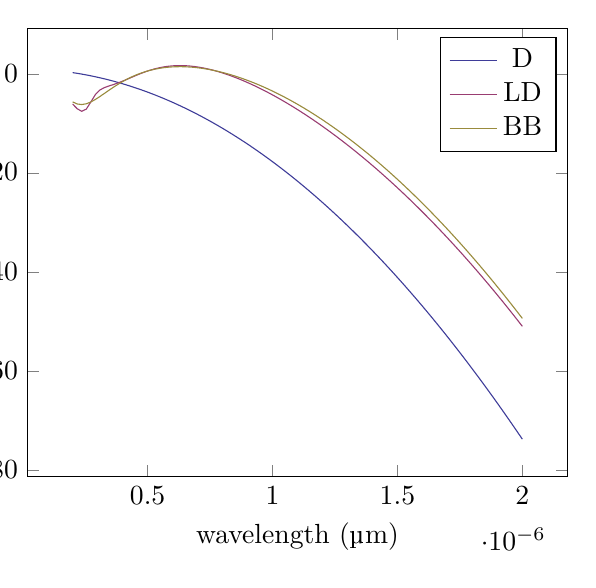
\begin{tikzpicture}[baseline,trim axis left]
\begin{axis}[xlabel=wavelength (\si{\micro\meter}),ylabel=$\epsilon'$]
\addplot[color=colora] coordinates {
(2e-07, 0.251131379491)
(2.18181818182e-07, 0.108789851357)
(2.36363636364e-07, -0.0459272446245)
(2.54545454545e-07, -0.213019419415)
(2.72727272727e-07, -0.39248614487)
(2.90909090909e-07, -0.584326853745)
(3.09090909091e-07, -0.788540939699)
(3.27272727273e-07, -1.0051277573)
(3.45454545455e-07, -1.23408662202)
(3.63636363636e-07, -1.47541681027)
(3.81818181818e-07, -1.72911755937)
(4e-07, -1.99518806757)
(4.18181818182e-07, -2.27362749407)
(4.36363636364e-07, -2.56443495899)
(4.54545454545e-07, -2.86760954344)
(4.72727272727e-07, -3.18315028944)
(4.90909090909e-07, -3.51105620002)
(5.09090909091e-07, -3.85132623914)
(5.27272727273e-07, -4.20395933178)
(5.45454545455e-07, -4.56895436389)
(5.63636363636e-07, -4.94631018242)
(5.81818181818e-07, -5.33602559533)
(6e-07, -5.7380993716)
(6.18181818182e-07, -6.15253024123)
(6.36363636364e-07, -6.57931689527)
(6.54545454545e-07, -7.0184579858)
(6.72727272727e-07, -7.46995212598)
(6.90909090909e-07, -7.93379789001)
(7.09090909091e-07, -8.40999381319)
(7.27272727273e-07, -8.89853839191)
(7.45454545455e-07, -9.39943008367)
(7.63636363636e-07, -9.91266730706)
(7.81818181818e-07, -10.4382484418)
(8e-07, -10.9761718288)
(8.18181818182e-07, -11.5264357701)
(8.36363636364e-07, -12.0890385289)
(8.54545454545e-07, -12.6639783295)
(8.72727272727e-07, -13.2512533576)
(8.90909090909e-07, -13.8508617599)
(9.09090909091e-07, -14.4628016444)
(9.27272727273e-07, -15.0870710803)
(9.45454545455e-07, -15.7236680983)
(9.63636363636e-07, -16.3725906899)
(9.81818181818e-07, -17.0338368084)
(1e-06, -17.707404368)
(1.01818181818e-06, -18.3932912445)
(1.03636363636e-06, -19.0914952747)
(1.05454545455e-06, -19.8020142572)
(1.07272727273e-06, -20.5248459517)
(1.09090909091e-06, -21.2599880791)
(1.10909090909e-06, -22.0074383222)
(1.12727272727e-06, -22.7671943248)
(1.14545454545e-06, -23.5392536923)
(1.16363636364e-06, -24.3236139915)
(1.18181818182e-06, -25.1202727509)
(1.2e-06, -25.9292274601)
(1.21818181818e-06, -26.7504755707)
(1.23636363636e-06, -27.5840144953)
(1.25454545455e-06, -28.4298416086)
(1.27272727273e-06, -29.2879542464)
(1.29090909091e-06, -30.1583497066)
(1.30909090909e-06, -31.0410252481)
(1.32727272727e-06, -31.9359780921)
(1.34545454545e-06, -32.843205421)
(1.36363636364e-06, -33.7627043791)
(1.38181818182e-06, -34.6944720723)
(1.4e-06, -35.6385055683)
(1.41818181818e-06, -36.5948018965)
(1.43636363636e-06, -37.5633580483)
(1.45454545455e-06, -38.5441709765)
(1.47272727273e-06, -39.537237596)
(1.49090909091e-06, -40.5425547836)
(1.50909090909e-06, -41.5601193779)
(1.52727272727e-06, -42.5899281792)
(1.54545454545e-06, -43.63197795)
(1.56363636364e-06, -44.6862654146)
(1.58181818182e-06, -45.7527872594)
(1.6e-06, -46.8315401327)
(1.61818181818e-06, -47.9225206449)
(1.63636363636e-06, -49.0257253683)
(1.65454545455e-06, -50.1411508375)
(1.67272727273e-06, -51.2687935491)
(1.69090909091e-06, -52.4086499617)
(1.70909090909e-06, -53.5607164964)
(1.72727272727e-06, -54.7249895361)
(1.74545454545e-06, -55.9014654263)
(1.76363636364e-06, -57.0901404745)
(1.78181818182e-06, -58.2910109504)
(1.8e-06, -59.5040730864)
(1.81818181818e-06, -60.7293230768)
(1.83636363636e-06, -61.9667570785)
(1.85454545455e-06, -63.2163712108)
(1.87272727273e-06, -64.4781615553)
(1.89090909091e-06, -65.7521241562)
(1.90909090909e-06, -67.0382550201)
(1.92727272727e-06, -68.336550116)
(1.94545454545e-06, -69.6470053759)
(1.96363636364e-06, -70.9696166938)
(1.98181818182e-06, -72.3043799266)
(2e-06, -73.651290894)
};
\addlegendentry{D}
\addplot[color=colorb] coordinates {
(2e-07, -6.08845577047)
(2.18181818182e-07, -7.02959345159)
(2.36363636364e-07, -7.54393219393)
(2.54545454545e-07, -7.11092481793)
(2.72727272727e-07, -5.67828154681)
(2.90909090909e-07, -4.17868107519)
(3.09090909091e-07, -3.25119424883)
(3.27272727273e-07, -2.76060684464)
(3.45454545455e-07, -2.44077157937)
(3.63636363636e-07, -2.14621282379)
(3.81818181818e-07, -1.82435335921)
(4e-07, -1.4670152428)
(4.18181818182e-07, -1.08380729028)
(4.36363636364e-07, -0.689858050171)
(4.54545454545e-07, -0.300423655924)
(4.72727272727e-07, 0.0713298952343)
(4.90909090909e-07, 0.415046559158)
(5.09090909091e-07, 0.723186997766)
(5.27272727273e-07, 0.990713298501)
(5.45454545455e-07, 1.21465542413)
(5.63636363636e-07, 1.39366570278)
(5.81818181818e-07, 1.52761351684)
(6e-07, 1.61724158882)
(6.18181818182e-07, 1.66388818931)
(6.36363636364e-07, 1.66927077814)
(6.54545454545e-07, 1.63532270587)
(6.72727272727e-07, 1.56407353746)
(6.90909090909e-07, 1.45756398528)
(7.09090909091e-07, 1.3177875484)
(7.27272727273e-07, 1.14665228397)
(7.45454545455e-07, 0.945957436856)
(7.63636363636e-07, 0.717380808514)
(7.81818181818e-07, 0.462473715875)
(8e-07, 0.182661174121)
(8.18181818182e-07, -0.120754446196)
(8.36363636364e-07, -0.446587562217)
(8.54545454545e-07, -0.793762236149)
(8.72727272727e-07, -1.16130439135)
(8.90909090909e-07, -1.54833383208)
(9.09090909091e-07, -1.95405636591)
(9.27272727273e-07, -2.37775622246)
(9.45454545455e-07, -2.81878888653)
(9.63636363636e-07, -3.27657441071)
(9.81818181818e-07, -3.75059123565)
(1e-06, -4.24037052128)
(1.01818181818e-06, -4.7454909759)
(1.03636363636e-06, -5.26557415943)
(1.05454545455e-06, -5.80028023171)
(1.07272727273e-06, -6.349304113)
(1.09090909091e-06, -6.91237202349)
(1.10909090909e-06, -7.48923836856)
(1.12727272727e-06, -8.07968293813)
(1.14545454545e-06, -8.68350838997)
(1.16363636364e-06, -9.30053798915)
(1.18181818182e-06, -9.93061357781)
(1.2e-06, -10.5735937518)
(1.21818181818e-06, -11.2293522227)
(1.23636363636e-06, -11.8977763464)
(1.25454545455e-06, -12.5787657999)
(1.27272727273e-06, -13.2722313918)
(1.29090909091e-06, -13.9780939917)
(1.30909090909e-06, -14.6962835662)
(1.32727272727e-06, -15.4267383106)
(1.34545454545e-06, -16.1694038655)
(1.36363636364e-06, -16.9242326107)
(1.38181818182e-06, -17.6911830268)
(1.4e-06, -18.4702191189)
(1.41818181818e-06, -19.2613098948)
(1.43636363636e-06, -20.0644288934)
(1.45454545455e-06, -20.879553757)
(1.47272727273e-06, -21.7066658433)
(1.49090909091e-06, -22.545749874)
(1.50909090909e-06, -23.3967936154)
(1.52727272727e-06, -24.259787588)
(1.54545454545e-06, -25.1347248022)
(1.56363636364e-06, -26.0216005184)
(1.58181818182e-06, -26.9204120278)
(1.6e-06, -27.8311584529)
(1.61818181818e-06, -28.7538405651)
(1.63636363636e-06, -29.688460619)
(1.65454545455e-06, -30.6350221998)
(1.67272727273e-06, -31.5935300851)
(1.69090909091e-06, -32.5639901177)
(1.70909090909e-06, -33.5464090888)
(1.72727272727e-06, -34.5407946324)
(1.74545454545e-06, -35.5471551271)
(1.76363636364e-06, -36.5654996068)
(1.78181818182e-06, -37.5958376785)
(1.8e-06, -38.6381794474)
(1.81818181818e-06, -39.6925354474)
(1.83636363636e-06, -40.7589165776)
(1.85454545455e-06, -41.8373340445)
(1.87272727273e-06, -42.9277993075)
(1.89090909091e-06, -44.0303240308)
(1.90909090909e-06, -45.144920037)
(1.92727272727e-06, -46.2715992667)
(1.94545454545e-06, -47.4103737391)
(1.96363636364e-06, -48.5612555179)
(1.98181818182e-06, -49.7242566784)
(2e-06, -50.8993892779)
};
\addlegendentry{LD}
\addplot[color=colorc] coordinates {
(2e-07, -5.64912808287)
(2.18181818182e-07, -6.07016971242)
(2.36363636364e-07, -6.18842750784)
(2.54545454545e-07, -6.03496184591)
(2.72727272727e-07, -5.67051946045)
(2.90909090909e-07, -5.1619489373)
(3.09090909091e-07, -4.568477678)
(3.27272727273e-07, -3.9366146404)
(3.45454545455e-07, -3.30007536217)
(3.63636363636e-07, -2.68183361787)
(3.81818181818e-07, -2.09665636586)
(4e-07, -1.55339411269)
(4.18181818182e-07, -1.05680141449)
(4.36363636364e-07, -0.608888393718)
(4.54545454545e-07, -0.209883482242)
(4.72727272727e-07, 0.141099404877)
(4.90909090909e-07, 0.445607912873)
(5.09090909091e-07, 0.705549121174)
(5.27272727273e-07, 0.922991644038)
(5.45454545455e-07, 1.10003880876)
(5.63636363636e-07, 1.23874979917)
(5.81818181818e-07, 1.34109285187)
(6e-07, 1.4089196413)
(6.18181818182e-07, 1.44395348173)
(6.36363636364e-07, 1.44778637023)
(6.54545454545e-07, 1.42188152981)
(6.72727272727e-07, 1.36757922474)
(6.90909090909e-07, 1.28610437492)
(7.09090909091e-07, 1.17857500763)
(7.27272727273e-07, 1.04601093008)
(7.45454545455e-07, 0.889342238251)
(7.63636363636e-07, 0.709417432978)
(7.81818181818e-07, 0.507011016743)
(8e-07, 0.282830512387)
(8.18181818182e-07, 0.0375228880207)
(8.36363636364e-07, -0.228319600415)
(8.54545454545e-07, -0.514154121357)
(8.72727272727e-07, -0.81948249811)
(8.90909090909e-07, -1.14384691695)
(9.09090909091e-07, -1.48682607117)
(9.27272727273e-07, -1.84803170008)
(9.45454545455e-07, -2.22710548427)
(9.63636363636e-07, -2.62371626063)
(9.81818181818e-07, -3.03755752401)
(1e-06, -3.46834518496)
(1.01818181818e-06, -3.91581555631)
(1.03636363636e-06, -4.37972354377)
(1.05454545455e-06, -4.85984101863)
(1.07272727273e-06, -5.35595535268)
(1.09090909091e-06, -5.86786809804)
(1.10909090909e-06, -6.39539379614)
(1.12727272727e-06, -6.93835890198)
(1.14545454545e-06, -7.49660081152)
(1.16363636364e-06, -8.0699669812)
(1.18181818182e-06, -8.65831412977)
(1.2e-06, -9.26150751417)
(1.21818181818e-06, -9.87942027139)
(1.23636363636e-06, -10.51193282)
(1.25454545455e-06, -11.1589323146)
(1.27272727273e-06, -11.8203121491)
(1.29090909091e-06, -12.4959715025)
(1.30909090909e-06, -13.1858149236)
(1.32727272727e-06, -13.8897519518)
(1.34545454545e-06, -14.6076967686)
(1.36363636364e-06, -15.3395678787)
(1.38181818182e-06, -16.0852878165)
(1.4e-06, -16.8447828767)
(1.41818181818e-06, -17.617982866)
(1.43636363636e-06, -18.4048208746)
(1.45454545455e-06, -19.2052330652)
(1.47272727273e-06, -20.0191584781)
(1.49090909091e-06, -20.8465388514)
(1.50909090909e-06, -21.6873184539)
(1.52727272727e-06, -22.5414439311)
(1.54545454545e-06, -23.4088641622)
(1.56363636364e-06, -24.2895301269)
(1.58181818182e-06, -25.1833947821)
(1.6e-06, -26.0904129473)
(1.61818181818e-06, -27.0105411977)
(1.63636363636e-06, -27.9437377647)
(1.65454545455e-06, -28.8899624432)
(1.67272727273e-06, -29.849176505)
(1.69090909091e-06, -30.821342618)
(1.70909090909e-06, -31.8064247705)
(1.72727272727e-06, -32.8043882005)
(1.74545454545e-06, -33.8151993298)
(1.76363636364e-06, -34.8388257016)
(1.78181818182e-06, -35.8752359226)
(1.8e-06, -36.9243996082)
(1.81818181818e-06, -37.9862873316)
(1.83636363636e-06, -39.0608705752)
(1.85454545455e-06, -40.1481216856)
(1.87272727273e-06, -41.2480138308)
(1.89090909091e-06, -42.3605209603)
(1.90909090909e-06, -43.4856177667)
(1.92727272727e-06, -44.6232796509)
(1.94545454545e-06, -45.7734826877)
(1.96363636364e-06, -46.9362035941)
(1.98181818182e-06, -48.1114196998)
(2e-06, -49.299108918)
};
\addlegendentry{BB}
\end{axis}
\end{tikzpicture}%
\\
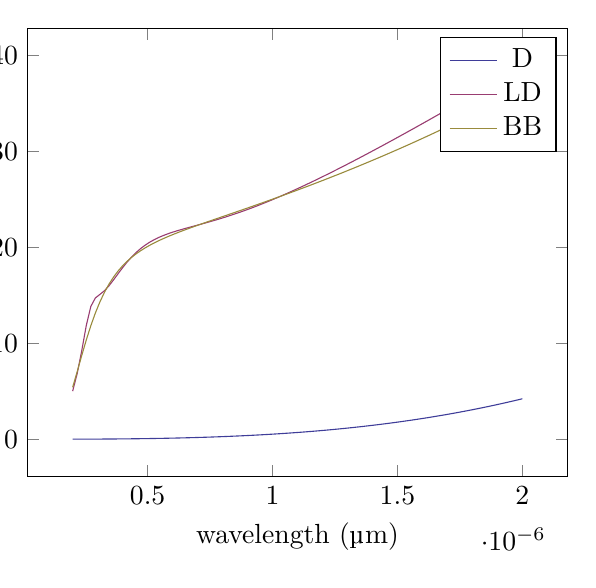
\begin{tikzpicture}[baseline,trim axis left]
\begin{axis}[xlabel=wavelength (\si{\micro\meter}),ylabel=$\epsilon''$]
\addplot[color=colora] coordinates {
(2e-07, 0.00422802312142)
(2.18181818182e-07, 0.00548909067452)
(2.36363636364e-07, 0.0069788499954)
(2.54545454545e-07, 0.00871635329274)
(2.72727272727e-07, 0.0107206514701)
(2.90909090909e-07, 0.0130107940258)
(3.09090909091e-07, 0.0156058289522)
(3.27272727273e-07, 0.0185248026359)
(3.45454545455e-07, 0.0217867597569)
(3.63636363636e-07, 0.0254107431891)
(3.81818181818e-07, 0.0294157938993)
(4e-07, 0.0338209508474)
(4.18181818182e-07, 0.0386452508862)
(4.36363636364e-07, 0.0439077286612)
(4.54545454545e-07, 0.0496274165104)
(4.72727272727e-07, 0.0558233443641)
(4.90909090909e-07, 0.0625145396451)
(5.09090909091e-07, 0.0697200271683)
(5.27272727273e-07, 0.0774588290411)
(5.45454545455e-07, 0.0857499645628)
(5.63636363636e-07, 0.0946124501251)
(5.81818181818e-07, 0.104065299112)
(6e-07, 0.1141275218)
(6.18181818182e-07, 0.124818125258)
(6.36363636364e-07, 0.136156113248)
(6.54545454545e-07, 0.148160486124)
(6.72727272727e-07, 0.160850240734)
(6.90909090909e-07, 0.17424437032)
(7.09090909091e-07, 0.188361864415)
(7.27272727273e-07, 0.203221708749)
(7.45454545455e-07, 0.218842885145)
(7.63636363636e-07, 0.235244371422)
(7.81818181818e-07, 0.252445141294)
(8e-07, 0.27046416427)
(8.18181818182e-07, 0.289320405556)
(8.36363636364e-07, 0.309032825955)
(8.54545454545e-07, 0.32962038177)
(8.72727272727e-07, 0.3511020247)
(8.90909090909e-07, 0.373496701743)
(9.09090909091e-07, 0.3968233551)
(9.27272727273e-07, 0.42110092207)
(9.45454545455e-07, 0.446348334955)
(9.63636363636e-07, 0.472584520961)
(9.81818181818e-07, 0.499828402097)
(1e-06, 0.528098895076)
(1.01818181818e-06, 0.557414911221)
(1.03636363636e-06, 0.587795356358)
(1.05454545455e-06, 0.619259130725)
(1.07272727273e-06, 0.651825128867)
(1.09090909091e-06, 0.685512239544)
(1.10909090909e-06, 0.720339345628)
(1.12727272727e-06, 0.756325324002)
(1.14545454545e-06, 0.793489045471)
(1.16363636364e-06, 0.831849374652)
(1.18181818182e-06, 0.871425169887)
(1.2e-06, 0.912235283134)
(1.21818181818e-06, 0.954298559878)
(1.23636363636e-06, 0.997633839028)
(1.25454545455e-06, 1.04225995282)
(1.27272727273e-06, 1.08819572672)
(1.29090909091e-06, 1.13545997932)
(1.30909090909e-06, 1.18407152225)
(1.32727272727e-06, 1.23404916009)
(1.34545454545e-06, 1.28541169023)
(1.36363636364e-06, 1.33817790281)
(1.38181818182e-06, 1.39236658064)
(1.4e-06, 1.44799649904)
(1.41818181818e-06, 1.5050864258)
(1.43636363636e-06, 1.56365512105)
(1.45454545455e-06, 1.62372133717)
(1.47272727273e-06, 1.68530381873)
(1.49090909091e-06, 1.74842130232)
(1.50909090909e-06, 1.81309251652)
(1.52727272727e-06, 1.87933618176)
(1.54545454545e-06, 1.94717101026)
(1.56363636364e-06, 2.01661570588)
(1.58181818182e-06, 2.0876889641)
(1.6e-06, 2.16040947184)
(1.61818181818e-06, 2.23479590744)
(1.63636363636e-06, 2.3108669405)
(1.65454545455e-06, 2.38864123183)
(1.67272727273e-06, 2.46813743333)
(1.69090909091e-06, 2.54937418789)
(1.70909090909e-06, 2.63237012932)
(1.72727272727e-06, 2.71714388224)
(1.74545454545e-06, 2.80371406195)
(1.76363636364e-06, 2.89209927442)
(1.78181818182e-06, 2.98231811609)
(1.8e-06, 3.07438917387)
(1.81818181818e-06, 3.16833102497)
(1.83636363636e-06, 3.26416223685)
(1.85454545455e-06, 3.36190136711)
(1.87272727273e-06, 3.46156696339)
(1.89090909091e-06, 3.56317756329)
(1.90909090909e-06, 3.66675169427)
(1.92727272727e-06, 3.77230787354)
(1.94545454545e-06, 3.87986460798)
(1.96363636364e-06, 3.98944039405)
(1.98181818182e-06, 4.10105371769)
(2e-06, 4.21472305421)
};
\addlegendentry{D}
\addplot[color=colorb] coordinates {
(2e-07, 5.00951113135)
(2.18181818182e-07, 6.843041516)
(2.36363636364e-07, 9.21811276848)
(2.54545454545e-07, 11.850165662)
(2.72727272727e-07, 13.838000528)
(2.90909090909e-07, 14.7250094569)
(3.09090909091e-07, 15.0948858637)
(3.27272727273e-07, 15.4770827886)
(3.45454545455e-07, 15.9944468664)
(3.63636363636e-07, 16.6059176112)
(3.81818181818e-07, 17.2498873727)
(4e-07, 17.8802887848)
(4.18181818182e-07, 18.4690187284)
(4.36363636364e-07, 19.0017011551)
(4.54545454545e-07, 19.4733125776)
(4.72727272727e-07, 19.884792185)
(4.90909090909e-07, 20.240607884)
(5.09090909091e-07, 20.5470738613)
(5.27272727273e-07, 20.8112287368)
(5.45454545455e-07, 21.0401213174)
(5.63636363636e-07, 21.2403853236)
(5.81818181818e-07, 21.4180128385)
(6e-07, 21.5782593971)
(6.18181818182e-07, 21.725632241)
(6.36363636364e-07, 21.8639277851)
(6.54545454545e-07, 21.9962953114)
(6.72727272727e-07, 22.1253119172)
(6.90909090909e-07, 22.2530594025)
(7.09090909091e-07, 22.381197658)
(7.27272727273e-07, 22.5110316831)
(7.45454545455e-07, 22.6435710035)
(7.63636363636e-07, 22.7795812595)
(7.81818181818e-07, 22.9196283143)
(8e-07, 23.0641155329)
(8.18181818182e-07, 23.2133150047)
(8.36363636364e-07, 23.3673935097)
(8.54545454545e-07, 23.5264339867)
(8.72727272727e-07, 23.6904531974)
(8.90909090909e-07, 23.8594162001)
(9.09090909091e-07, 24.0332481623)
(9.27272727273e-07, 24.2118439696)
(9.45454545455e-07, 24.3950760124)
(9.63636363636e-07, 24.5828004727)
(9.81818181818e-07, 24.774862381)
(1e-06, 24.9710996636)
(1.01818181818e-06, 25.1713463661)
(1.03636363636e-06, 25.3754352037)
(1.05454545455e-06, 25.5831995632)
(1.07272727273e-06, 25.7944750603)
(1.09090909091e-06, 26.009100734)
(1.10909090909e-06, 26.226919949)
(1.12727272727e-06, 26.4477810619)
(1.14545454545e-06, 26.6715378956)
(1.16363636364e-06, 26.8980500628)
(1.18181818182e-06, 27.1271831657)
(1.2e-06, 27.3588089001)
(1.21818181818e-06, 27.5928050819)
(1.23636363636e-06, 27.829055614)
(1.25454545455e-06, 28.0674504074)
(1.27272727273e-06, 28.3078852653)
(1.29090909091e-06, 28.5502617425)
(1.30909090909e-06, 28.7944869837)
(1.32727272727e-06, 29.0404735491)
(1.34545454545e-06, 29.2881392306)
(1.36363636364e-06, 29.5374068628)
(1.38181818182e-06, 29.7882041312)
(1.4e-06, 30.0404633809)
(1.41818181818e-06, 30.2941214263)
(1.43636363636e-06, 30.5491193642)
(1.45454545455e-06, 30.8054023911)
(1.47272727273e-06, 31.0629196251)
(1.49090909091e-06, 31.3216239335)
(1.50909090909e-06, 31.5814717659)
(1.52727272727e-06, 31.8424229934)
(1.54545454545e-06, 32.1044407545)
(1.56363636364e-06, 32.3674913066)
(1.58181818182e-06, 32.6315438838)
(1.6e-06, 32.896570561)
(1.61818181818e-06, 33.1625461241)
(1.63636363636e-06, 33.4294479454)
(1.65454545455e-06, 33.6972558654)
(1.67272727273e-06, 33.9659520793)
(1.69090909091e-06, 34.2355210294)
(1.70909090909e-06, 34.5059493024)
(1.72727272727e-06, 34.7772255308)
(1.74545454545e-06, 35.0493402999)
(1.76363636364e-06, 35.3222860587)
(1.78181818182e-06, 35.5960570346)
(1.8e-06, 35.8706491532)
(1.81818181818e-06, 36.1460599604)
(1.83636363636e-06, 36.4222885494)
(1.85454545455e-06, 36.6993354906)
(1.87272727273e-06, 36.9772027643)
(1.89090909091e-06, 37.2558936973)
(1.90909090909e-06, 37.5354129019)
(1.92727272727e-06, 37.8157662176)
(1.94545454545e-06, 38.0969606562)
(1.96363636364e-06, 38.3790043479)
(1.98181818182e-06, 38.6619064917)
(2e-06, 38.9456773061)
};
\addlegendentry{LD}
\addplot[color=colorc] coordinates {
(2e-07, 5.40716550663)
(2.18181818182e-07, 7.04484300503)
(2.36363636364e-07, 8.72402440718)
(2.54545454545e-07, 10.341082493)
(2.72727272727e-07, 11.8283829865)
(2.90909090909e-07, 13.1537495401)
(3.09090909091e-07, 14.3109689131)
(3.27272727273e-07, 15.3093894963)
(3.45454545455e-07, 16.1659394498)
(3.63636363636e-07, 16.9000194757)
(3.81818181818e-07, 17.5306493657)
(4e-07, 18.0750945048)
(4.18181818182e-07, 18.5483617298)
(4.36363636364e-07, 18.9631596763)
(4.54545454545e-07, 19.330080446)
(4.72727272727e-07, 19.6578667803)
(4.90909090909e-07, 19.9536940427)
(5.09090909091e-07, 20.2234334901)
(5.27272727273e-07, 20.4718834781)
(5.45454545455e-07, 20.7029655987)
(5.63636363636e-07, 20.9198876504)
(5.81818181818e-07, 21.1252773381)
(6e-07, 21.3212911166)
(6.18181818182e-07, 21.5097024034)
(6.36363636364e-07, 21.6919729082)
(6.54545454545e-07, 21.869310264)
(6.72727272727e-07, 22.042714603)
(6.90909090909e-07, 22.213016235)
(7.09090909091e-07, 22.3809061725)
(7.27272727273e-07, 22.5469609075)
(7.45454545455e-07, 22.711662564)
(7.63636363636e-07, 22.8754153265)
(7.81818181818e-07, 23.0385588644)
(8e-07, 23.201379327)
(8.18181818182e-07, 23.3641183731)
(8.36363636364e-07, 23.5269806014)
(8.54545454545e-07, 23.6901396828)
(8.72727272727e-07, 23.8537434305)
(8.90909090909e-07, 24.0179180042)
(9.09090909091e-07, 24.1827714019)
(9.27272727273e-07, 24.3483963679)
(9.45454545455e-07, 24.5148728188)
(9.63636363636e-07, 24.6822698725)
(9.81818181818e-07, 24.850647547)
(1e-06, 25.0200581868)
(1.01818181818e-06, 25.190547662)
(1.03636363636e-06, 25.362156378)
(1.05454545455e-06, 25.5349201274)
(1.07272727273e-06, 25.7088708093)
(1.09090909091e-06, 25.8840370384)
(1.10909090909e-06, 26.0604446599)
(1.12727272727e-06, 26.238117187)
(1.14545454545e-06, 26.4170761719)
(1.16363636364e-06, 26.5973415209)
(1.18181818182e-06, 26.7789317628)
(1.2e-06, 26.9618642764)
(1.21818181818e-06, 27.1461554849)
(1.23636363636e-06, 27.3318210214)
(1.25454545455e-06, 27.5188758694)
(1.27272727273e-06, 27.7073344827)
(1.29090909091e-06, 27.8972108879)
(1.30909090909e-06, 28.0885187708)
(1.32727272727e-06, 28.2812715505)
(1.34545454545e-06, 28.4754824422)
(1.36363636364e-06, 28.6711645106)
(1.38181818182e-06, 28.8683307151)
(1.4e-06, 29.0669939475)
(1.41818181818e-06, 29.2671670649)
(1.43636363636e-06, 29.4688629161)
(1.45454545455e-06, 29.6720943648)
(1.47272727273e-06, 29.8768743081)
(1.49090909091e-06, 30.0832156922)
(1.50909090909e-06, 30.2911315255)
(1.52727272727e-06, 30.5006348888)
(1.54545454545e-06, 30.7117389438)
(1.56363636364e-06, 30.92445694)
(1.58181818182e-06, 31.1388022193)
(1.6e-06, 31.3547882206)
(1.61818181818e-06, 31.5724284822)
(1.63636363636e-06, 31.7917366438)
(1.65454545455e-06, 32.0127264475)
(1.67272727273e-06, 32.2354117383)
(1.69090909091e-06, 32.4598064639)
(1.70909090909e-06, 32.6859246741)
(1.72727272727e-06, 32.9137805199)
(1.74545454545e-06, 33.1433882521)
(1.76363636364e-06, 33.3747622193)
(1.78181818182e-06, 33.6079168668)
(1.8e-06, 33.8428667339)
(1.81818181818e-06, 34.0796264521)
(1.83636363636e-06, 34.3182107427)
(1.85454545455e-06, 34.5586344145)
(1.87272727273e-06, 34.8009123614)
(1.89090909091e-06, 35.0450595599)
(1.90909090909e-06, 35.2910910663)
(1.92727272727e-06, 35.539022015)
(1.94545454545e-06, 35.7888676152)
(1.96363636364e-06, 36.0406431488)
(1.98181818182e-06, 36.2943639679)
(2e-06, 36.5500454925)
};
\addlegendentry{BB}
\end{axis}
\end{tikzpicture}%
\\
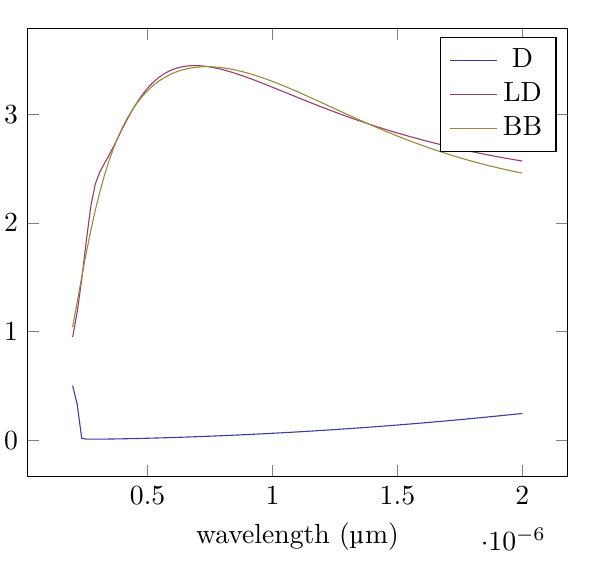
\begin{tikzpicture}[baseline,trim axis left]
\begin{axis}[xlabel=wavelength (\si{\micro\meter}),ylabel=$n'$]
\addplot[color=colora] coordinates {
(2e-07, 0.501147856301)
(2.18181818182e-07, 0.329937943572)
(2.36363636364e-07, 0.0162358824354)
(2.54545454545e-07, 0.00944070431963)
(2.72727272727e-07, 0.00855536464497)
(2.90909090909e-07, 0.00850979255711)
(3.09090909091e-07, 0.0087866527669)
(3.27272727273e-07, 0.00923835237168)
(3.45454545455e-07, 0.00980557145985)
(3.63636363636e-07, 0.0104595718314)
(3.81818181818e-07, 0.0111846554101)
(4e-07, 0.0119714925836)
(4.18181818182e-07, 0.0128141793232)
(4.36363636364e-07, 0.0137087930079)
(4.54545454545e-07, 0.0146526240186)
(4.72727272727e-07, 0.0156437400149)
(4.90909090909e-07, 0.0166807257925)
(5.09090909091e-07, 0.0177625212056)
(5.27272727273e-07, 0.0188883164976)
(5.45454545455e-07, 0.0200574826037)
(5.63636363636e-07, 0.0212695234942)
(5.81818181818e-07, 0.0225240428273)
(6e-07, 0.0238207201344)
(6.18181818182e-07, 0.0251592935013)
(6.36363636364e-07, 0.0265395467701)
(6.54545454545e-07, 0.0279612999416)
(6.72727272727e-07, 0.0294244018829)
(6.90909090909e-07, 0.0309287247204)
(7.09090909091e-07, 0.0324741594808)
(7.27272727273e-07, 0.0340606126682)
(7.45454545455e-07, 0.035688003552)
(7.63636363636e-07, 0.0373562619986)
(7.81818181818e-07, 0.0390653267256)
(8e-07, 0.0408151438846)
(8.18181818182e-07, 0.0426056659029)
(8.36363636364e-07, 0.0444368505324)
(8.54545454545e-07, 0.0463086600613)
(8.72727272727e-07, 0.0482210606597)
(8.90909090909e-07, 0.0501740218317)
(9.09090909091e-07, 0.0521675159556)
(9.27272727273e-07, 0.0542015178946)
(9.45454545455e-07, 0.0562760046681)
(9.63636363636e-07, 0.0583909551708)
(9.81818181818e-07, 0.060546349933)
(1e-06, 0.0627421709146)
(1.01818181818e-06, 0.0649784013281)
(1.03636363636e-06, 0.0672550254855)
(1.05454545455e-06, 0.0695720286651)
(1.07272727273e-06, 0.0719293969965)
(1.09090909091e-06, 0.0743271173598)
(1.10909090909e-06, 0.0767651772973)
(1.12727272727e-06, 0.0792435649364)
(1.14545454545e-06, 0.0817622689217)
(1.16363636364e-06, 0.084321278355)
(1.18181818182e-06, 0.0869205827427)
(1.2e-06, 0.0895601719484)
(1.21818181818e-06, 0.092240036152)
(1.23636363636e-06, 0.094960165812)
(1.25454545455e-06, 0.097720551633)
(1.27272727273e-06, 0.100521184536)
(1.29090909091e-06, 0.103362055633)
(1.30909090909e-06, 0.106243156201)
(1.32727272727e-06, 0.109164477663)
(1.34545454545e-06, 0.11212601157)
(1.36363636364e-06, 0.115127749579)
(1.38181818182e-06, 0.118169683443)
(1.4e-06, 0.121251804994)
(1.41818181818e-06, 0.12437410613)
(1.43636363636e-06, 0.127536578805)
(1.45454545455e-06, 0.130739215019)
(1.47272727273e-06, 0.133982006806)
(1.49090909091e-06, 0.137264946228)
(1.50909090909e-06, 0.140588025364)
(1.52727272727e-06, 0.143951236308)
(1.54545454545e-06, 0.147354571156)
(1.56363636364e-06, 0.150798022005)
(1.58181818182e-06, 0.154281580946)
(1.6e-06, 0.157805240057)
(1.61818181818e-06, 0.161368991403)
(1.63636363636e-06, 0.164972827027)
(1.65454545455e-06, 0.168616738947)
(1.67272727273e-06, 0.172300719155)
(1.69090909091e-06, 0.176024759613)
(1.70909090909e-06, 0.179788852248)
(1.72727272727e-06, 0.183592988948)
(1.74545454545e-06, 0.187437161566)
(1.76363636364e-06, 0.19132136191)
(1.78181818182e-06, 0.195245581746)
(1.8e-06, 0.199209812793)
(1.81818181818e-06, 0.203214046723)
(1.83636363636e-06, 0.207258275157)
(1.85454545455e-06, 0.211342489666)
(1.87272727273e-06, 0.215466681768)
(1.89090909091e-06, 0.219630842926)
(1.90909090909e-06, 0.22383496455)
(1.92727272727e-06, 0.22807903799)
(1.94545454545e-06, 0.232363054541)
(1.96363636364e-06, 0.236687005437)
(1.98181818182e-06, 0.241050881854)
(2e-06, 0.245454674906)
};
\addlegendentry{D}
\addplot[color=colorb] coordinates {
(2e-07, 0.947626154005)
(2.18181818182e-07, 1.17913691095)
(2.36363636364e-07, 1.47776799694)
(2.54545454545e-07, 1.8315361121)
(2.72727272727e-07, 2.15399978813)
(2.90909090909e-07, 2.35878831123)
(3.09090909091e-07, 2.46879017573)
(3.27272727273e-07, 2.54565800807)
(3.45454545455e-07, 2.62095744403)
(3.63636363636e-07, 2.70164975586)
(3.81818181818e-07, 2.78583361224)
(4e-07, 2.86996117913)
(4.18181818182e-07, 2.95101544746)
(4.36363636364e-07, 3.02690945131)
(4.54545454545e-07, 3.09638548715)
(4.72727272727e-07, 3.15881702664)
(4.90909090909e-07, 3.21402468822)
(5.09090909091e-07, 3.2621299621)
(5.27272727273e-07, 3.30344592954)
(5.45454545455e-07, 3.3383984837)
(5.63636363636e-07, 3.36747114921)
(5.81818181818e-07, 3.39116755919)
(6e-07, 3.40998683371)
(6.18181818182e-07, 3.42440818863)
(6.36363636364e-07, 3.43488201056)
(6.54545454545e-07, 3.44182535763)
(6.72727272727e-07, 3.44562040745)
(6.90909090909e-07, 3.44661479908)
(7.09090909091e-07, 3.44512313243)
(7.27272727273e-07, 3.44142911902)
(7.45454545455e-07, 3.43578804481)
(7.63636363636e-07, 3.42842932296)
(7.81818181818e-07, 3.41955899696)
(8e-07, 3.40936211099)
(8.18181818182e-07, 3.39800490255)
(8.36363636364e-07, 3.38563679775)
(8.54545454545e-07, 3.3723922058)
(8.72727272727e-07, 3.35839211962)
(8.90909090909e-07, 3.34374553484)
(9.09090909091e-07, 3.32855070299)
(9.27272727273e-07, 3.3128962356)
(9.45454545455e-07, 3.29686207584)
(9.63636363636e-07, 3.2805203538)
(9.81818181818e-07, 3.26393614026)
(1e-06, 3.24716811227)
(1.01818181818e-06, 3.23026914273)
(1.03636363636e-06, 3.21328682444)
(1.05454545455e-06, 3.19626393775)
(1.07272727273e-06, 3.17923886992)
(1.09090909091e-06, 3.16224599286)
(1.10909090909e-06, 3.1453160049)
(1.12727272727e-06, 3.12847624164)
(1.14545454545e-06, 3.11175095969)
(1.16363636364e-06, 3.09516159688)
(1.18181818182e-06, 3.07872701145)
(1.2e-06, 3.06246370291)
(1.21818181818e-06, 3.04638601602)
(1.23636363636e-06, 3.0305063299)
(1.25454545455e-06, 3.01483523322)
(1.27272727273e-06, 2.99938168683)
(1.29090909091e-06, 2.98415317461)
(1.30909090909e-06, 2.9691558434)
(1.32727272727e-06, 2.95439463268)
(1.34545454545e-06, 2.93987339471)
(1.36363636364e-06, 2.92559500553)
(1.38181818182e-06, 2.9115614675)
(1.4e-06, 2.89777400382)
(1.41818181818e-06, 2.88423314543)
(1.43636363636e-06, 2.87093881085)
(1.45454545455e-06, 2.85789037923)
(1.47272727273e-06, 2.84508675724)
(1.49090909091e-06, 2.83252643996)
(1.50909090909e-06, 2.82020756631)
(1.52727272727e-06, 2.80812796937)
(1.54545454545e-06, 2.7962852219)
(1.56363636364e-06, 2.78467667745)
(1.58181818182e-06, 2.77329950734)
(1.6e-06, 2.76215073391)
(1.61818181818e-06, 2.75122726026)
(1.63636363636e-06, 2.74052589674)
(1.65454545455e-06, 2.73004338461)
(1.67272727273e-06, 2.71977641695)
(1.69090909091e-06, 2.70972165709)
(1.70909090909e-06, 2.69987575492)
(1.72727272727e-06, 2.69023536106)
(1.74545454545e-06, 2.68079713929)
(1.76363636364e-06, 2.67155777728)
(1.78181818182e-06, 2.66251399582)
(1.8e-06, 2.65366255674)
(1.81818181818e-06, 2.64500026959)
(1.83636363636e-06, 2.63652399726)
(1.85454545455e-06, 2.62823066064)
(1.87272727273e-06, 2.62011724238)
(1.89090909091e-06, 2.61218078995)
(1.90909090909e-06, 2.60441841798)
(1.92727272727e-06, 2.59682730997)
(1.94545454545e-06, 2.58940471957)
(1.96363636364e-06, 2.58214797132)
(1.98181818182e-06, 2.57505446097)
(2e-06, 2.56812165556)
};
\addlegendentry{LD}
\addplot[color=colorc] coordinates {
(2e-07, 1.0418070887)
(2.18181818182e-07, 1.27065320754)
(2.36363636364e-07, 1.50126794164)
(2.54545454545e-07, 1.72312066603)
(2.72727272727e-07, 1.92961810184)
(2.90909090909e-07, 2.11759331866)
(3.09090909091e-07, 2.28626326847)
(3.27272727273e-07, 2.43626758513)
(3.45454545455e-07, 2.56897458702)
(3.63636363636e-07, 2.68604267768)
(3.81818181818e-07, 2.78916899046)
(4e-07, 2.87995901173)
(4.18181818182e-07, 2.95986839192)
(4.36363636364e-07, 3.0301851567)
(4.54545454545e-07, 3.09203301841)
(4.72727272727e-07, 3.14638463695)
(4.90909090909e-07, 3.19407866339)
(5.09090909091e-07, 3.23583732303)
(5.27272727273e-07, 3.2722829551)
(5.45454545455e-07, 3.30395283999)
(5.63636363636e-07, 3.33131212959)
(5.81818181818e-07, 3.35476493867)
(6e-07, 3.3746637643)
(6.18181818182e-07, 3.39131743894)
(6.36363636364e-07, 3.40499782395)
(6.54545454545e-07, 3.41594543518)
(6.72727272727e-07, 3.42437417023)
(6.90909090909e-07, 3.43047528295)
(7.09090909091e-07, 3.43442072875)
(7.27272727273e-07, 3.43636598396)
(7.45454545455e-07, 3.43645242538)
(7.63636363636e-07, 3.43480934121)
(7.81818181818e-07, 3.43155563247)
(8e-07, 3.42680125351)
(8.18181818182e-07, 3.4206484321)
(8.36363636364e-07, 3.41319270248)
(8.54545454545e-07, 3.40452377904)
(8.72727272727e-07, 3.39472629392)
(8.90909090909e-07, 3.38388041764)
(9.09090909091e-07, 3.37206237936)
(9.27272727273e-07, 3.35934490024)
(9.45454545455e-07, 3.34579755189)
(9.63636363636e-07, 3.33148705)
(9.81818181818e-07, 3.31647749188)
(1e-06, 3.30083054577)
(1.01818181818e-06, 3.28460559869)
(1.03636363636e-06, 3.26785986898)
(1.05454545455e-06, 3.25064848916)
(1.07272727273e-06, 3.23302456396)
(1.09090909091e-06, 3.21503920831)
(1.10909090909e-06, 3.19674156928)
(1.12727272727e-06, 3.17817883586)
(1.14545454545e-06, 3.15939623998)
(1.16363636364e-06, 3.14043705195)
(1.18181818182e-06, 3.12134257287)
(1.2e-06, 3.10215212661)
(1.21818181818e-06, 3.0829030533)
(1.23636363636e-06, 3.0636307061)
(1.25454545455e-06, 3.04436845254)
(1.27272727273e-06, 3.02514768163)
(1.29090909091e-06, 3.00599781737)
(1.30909090909e-06, 2.98694633921)
(1.32727272727e-06, 2.96801880965)
(1.34545454545e-06, 2.94923890896)
(1.36363636364e-06, 2.93062847676)
(1.38181818182e-06, 2.91220756016)
(1.4e-06, 2.8939944678)
(1.41818181818e-06, 2.87600582933)
(1.43636363636e-06, 2.85825665939)
(1.45454545455e-06, 2.84076042559)
(1.47272727273e-06, 2.82352911946)
(1.49090909091e-06, 2.80657332984)
(1.50909090909e-06, 2.78990231768)
(1.52727272727e-06, 2.77352409184)
(1.54545454545e-06, 2.75744548489)
(1.56363636364e-06, 2.74167222857)
(1.58181818182e-06, 2.72620902823)
(1.6e-06, 2.7110596357)
(1.61818181818e-06, 2.69622692033)
(1.63636363636e-06, 2.68171293774)
(1.65454545455e-06, 2.66751899603)
(1.67272727273e-06, 2.65364571916)
(1.69090909091e-06, 2.64009310748)
(1.70909090909e-06, 2.62686059511)
(1.72727272727e-06, 2.61394710426)
(1.74545454545e-06, 2.60135109629)
(1.76363636364e-06, 2.58907061975)
(1.78181818182e-06, 2.57710335518)
(1.8e-06, 2.56544665691)
(1.81818181818e-06, 2.55409759191)
(1.83636363636e-06, 2.54305297567)
(1.85454545455e-06, 2.53230940547)
(1.87272727273e-06, 2.52186329084)
(1.89090909091e-06, 2.5117108817)
(1.90909090909e-06, 2.50184829396)
(1.92727272727e-06, 2.49227153297)
(1.94545454545e-06, 2.48297651487)
(1.96363636364e-06, 2.47395908596)
(1.98181818182e-06, 2.4652150402)
(2e-06, 2.45674013506)
};
\addlegendentry{BB}
\end{axis}
\end{tikzpicture}%
\\
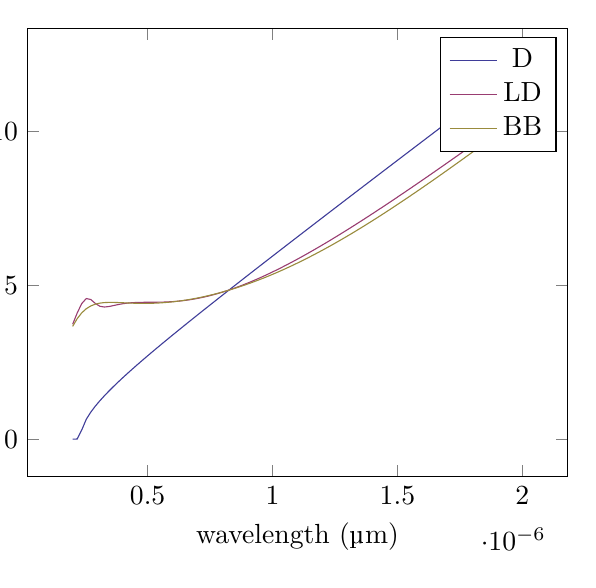
\begin{tikzpicture}[baseline,trim axis left]
\begin{axis}[xlabel=wavelength (\si{\micro\meter}),ylabel=$n''$]
\addplot[color=colora] coordinates {
(2e-07, 0.00596563226317)
(2.18181818182e-07, 0.0117639492945)
(2.36363636364e-07, 0.303943575365)
(2.54545454545e-07, 0.652853040604)
(2.72727272727e-07, 0.886069228824)
(2.90909090909e-07, 1.0811098652)
(3.09090909091e-07, 1.255880683)
(3.27272727273e-07, 1.4178949922)
(3.45454545455e-07, 1.5711032883)
(3.63636363636e-07, 1.71786274941)
(3.81818181818e-07, 1.85970032849)
(4e-07, 1.99766432826)
(4.18181818182e-07, 2.13250636447)
(4.36363636364e-07, 2.26478382633)
(4.54545454545e-07, 2.39492139446)
(4.72727272727e-07, 2.5232498949)
(4.90909090909e-07, 2.65003186646)
(5.09090909091e-07, 2.77547896634)
(5.27272727273e-07, 2.89976416292)
(5.45454545455e-07, 3.02303048827)
(5.63636363636e-07, 3.14539745503)
(5.81818181818e-07, 3.26696584856)
(6e-07, 3.38782136433)
(6.18181818182e-07, 3.50803740895)
(6.36363636364e-07, 3.62767728521)
(6.54545454545e-07, 3.74679591654)
(6.72727272727e-07, 3.86544122227)
(6.90909090909e-07, 3.98365522505)
(7.09090909091e-07, 4.10147495036)
(7.27272727273e-07, 4.21893316308)
(7.45454545455e-07, 4.33605897498)
(7.63636363636e-07, 4.45287834942)
(7.81818181818e-07, 4.56941452302)
(8e-07, 4.68568836028)
(8.18181818182e-07, 4.80171865334)
(8.36363636364e-07, 4.91752237668)
(8.54545454545e-07, 5.03311490462)
(8.72727272727e-07, 5.14851019777)
(8.90909090909e-07, 5.26372096379)
(9.09090909091e-07, 5.37875879624)
(9.27272727273e-07, 5.49363429523)
(9.45454545455e-07, 5.60835717246)
(9.63636363636e-07, 5.7229363431)
(9.81818181818e-07, 5.83738000628)
(1e-06, 5.95169571602)
(1.01818181818e-06, 6.06589044364)
(1.03636363636e-06, 6.17997063313)
(1.05454545455e-06, 6.2939422502)
(1.07272727273e-06, 6.40781082583)
(1.09090909091e-06, 6.52158149524)
(1.10909090909e-06, 6.63525903257)
(1.12727272727e-06, 6.74884788203)
(1.14545454545e-06, 6.86235218579)
(1.16363636364e-06, 6.97577580911)
(1.18181818182e-06, 7.08912236297)
(1.2e-06, 7.20239522444)
(1.21818181818e-06, 7.31559755521)
(1.23636363636e-06, 7.42873231829)
(1.25454545455e-06, 7.54180229319)
(1.27272727273e-06, 7.65481008974)
(1.29090909091e-06, 7.76775816064)
(1.30909090909e-06, 7.88064881293)
(1.32727272727e-06, 7.99348421845)
(1.34545454545e-06, 8.10626642339)
(1.36363636364e-06, 8.21899735708)
(1.38181818182e-06, 8.33167883999)
(1.4e-06, 8.44431259115)
(1.41818181818e-06, 8.55690023488)
(1.43636363636e-06, 8.66944330706)
(1.45454545455e-06, 8.7819432609)
(1.47272727273e-06, 8.89440147218)
(1.49090909091e-06, 9.00681924423)
(1.50909090909e-06, 9.11919781239)
(1.52727272727e-06, 9.23153834825)
(1.54545454545e-06, 9.34384196352)
(1.56363636364e-06, 9.45610971363)
(1.58181818182e-06, 9.56834260106)
(1.6e-06, 9.6805415785)
(1.61818181818e-06, 9.79270755167)
(1.63636363636e-06, 9.90484138207)
(1.65454545455e-06, 10.0169438894)
(1.67272727273e-06, 10.1290158542)
(1.69090909091e-06, 10.2410580193)
(1.70909090909e-06, 10.3530710929)
(1.72727272727e-06, 10.4650557497)
(1.74545454545e-06, 10.5770126327)
(1.76363636364e-06, 10.6889423553)
(1.78181818182e-06, 10.8008455028)
(1.8e-06, 10.9127226333)
(1.81818181818e-06, 11.0245742798)
(1.83636363636e-06, 11.136400951)
(1.85454545455e-06, 11.2482031328)
(1.87272727273e-06, 11.3599812893)
(1.89090909091e-06, 11.4717358637)
(1.90909090909e-06, 11.5834672798)
(1.92727272727e-06, 11.6951759426)
(1.94545454545e-06, 11.806862239)
(1.96363636364e-06, 11.9185265392)
(1.98181818182e-06, 12.030169197)
(2e-06, 12.1417905509)
};
\addlegendentry{D}
\addplot[color=colorb] coordinates {
(2e-07, 3.73803453655)
(2.18181818182e-07, 4.10364650192)
(2.36363636364e-07, 4.41083448946)
(2.54545454545e-07, 4.575029912)
(2.72727272727e-07, 4.5426856889)
(2.90909090909e-07, 4.41419604739)
(3.09090909091e-07, 4.32345213472)
(3.27272727273e-07, 4.29906537254)
(3.45454545455e-07, 4.31513371815)
(3.63636363636e-07, 4.34629134484)
(3.81818181818e-07, 4.37840662212)
(4e-07, 4.40538134843)
(4.18181818182e-07, 4.42544900805)
(4.36363636364e-07, 4.43892754539)
(4.54545454545e-07, 4.44702748832)
(4.72727272727e-07, 4.4512459183)
(4.90909090909e-07, 4.45306818662)
(5.09090909091e-07, 4.45383091099)
(5.27272727273e-07, 4.4546698443)
(5.45454545455e-07, 4.45651186733)
(5.63636363636e-07, 4.46008884171)
(5.81818181818e-07, 4.46596101588)
(6e-07, 4.47454324312)
(6.18181818182e-07, 4.48613046021)
(6.36363636364e-07, 4.50092071654)
(6.54545454545e-07, 4.51903509315)
(6.72727272727e-07, 4.54053442995)
(6.90909090909e-07, 4.5654330765)
(7.09090909091e-07, 4.59371001462)
(7.27272727273e-07, 4.62531773984)
(7.45454545455e-07, 4.6601892777)
(7.63636363636e-07, 4.69824367483)
(7.81818181818e-07, 4.7393902599)
(8e-07, 4.78353192312)
(8.18181818182e-07, 4.83056761964)
(8.36363636364e-07, 4.8803942645)
(8.54545454545e-07, 4.9329081536)
(8.72727272727e-07, 4.98800601854)
(8.90909090909e-07, 5.04558580025)
(9.09090909091e-07, 5.10554720834)
(9.27272727273e-07, 5.16779211856)
(9.45454545455e-07, 5.23222484869)
(9.63636363636e-07, 5.29875234417)
(9.81818181818e-07, 5.36728429717)
(1e-06, 5.43773321718)
(1.01818181818e-06, 5.51001446648)
(1.03636363636e-06, 5.5840462705)
(1.05454545455e-06, 5.65974971027)
(1.07272727273e-06, 5.73704870208)
(1.09090909091e-06, 5.81586996808)
(1.10909090909e-06, 5.89614300017)
(1.12727272727e-06, 5.97780001884)
(1.14545454545e-06, 6.06077592807)
(1.16363636364e-06, 6.14500826687)
(1.18181818182e-06, 6.23043715783)
(1.2e-06, 6.31700525303)
(1.21818181818e-06, 6.40465767724)
(1.23636363636e-06, 6.49334196881)
(1.25454545455e-06, 6.58300801813)
(1.27272727273e-06, 6.67360800394)
(1.29090909091e-06, 6.76509632766)
(1.30909090909e-06, 6.85742954592)
(1.32727272727e-06, 6.95056630156)
(1.34545454545e-06, 7.04446725344)
(1.36363636364e-06, 7.13909500526)
(1.38181818182e-06, 7.23441403374)
(1.4e-06, 7.33039061661)
(1.41818181818e-06, 7.42699276046)
(1.43636363636e-06, 7.52419012905)
(1.45454545455e-06, 7.62195397214)
(1.47272727273e-06, 7.72025705524)
(1.49090909091e-06, 7.81907359053)
(1.50909090909e-06, 7.91837916906)
(1.52727272727e-06, 8.01815069456)
(1.54545454545e-06, 8.11836631896)
(1.56363636364e-06, 8.21900537977)
(1.58181818182e-06, 8.32004833943)
(1.6e-06, 8.42147672677)
(1.61818181818e-06, 8.52327308054)
(1.63636363636e-06, 8.6254208952)
(1.65454545455e-06, 8.72790456887)
(1.67272727273e-06, 8.83070935354)
(1.69090909091e-06, 8.93382130743)
(1.70909090909e-06, 9.03722724964)
(1.72727272727e-06, 9.14091471685)
(1.74545454545e-06, 9.24487192222)
(1.76363636364e-06, 9.34908771636)
(1.78181818182e-06, 9.45355155023)
(1.8e-06, 9.55825344008)
(1.81818181818e-06, 9.66318393424)
(1.83636363636e-06, 9.76833408169)
(1.85454545455e-06, 9.87369540243)
(1.87272727273e-06, 9.97925985946)
(1.89090909091e-06, 10.0850198324)
(1.90909090909e-06, 10.1909680927)
(1.92727272727e-06, 10.2970977799)
(1.94545454545e-06, 10.4034023801)
(1.96363636364e-06, 10.5098757047)
(1.98181818182e-06, 10.6165118712)
(2e-06, 10.7233052848)
};
\addlegendentry{LD}
\addplot[color=colorc] coordinates {
(2e-07, 3.67001092449)
(2.18181818182e-07, 3.92039010463)
(2.36363636364e-07, 4.10907117009)
(2.54545454545e-07, 4.24360852945)
(2.72727272727e-07, 4.33450008177)
(2.90909090909e-07, 4.39230017202)
(3.09090909091e-07, 4.42616705757)
(3.27272727273e-07, 4.4434253424)
(3.45454545455e-07, 4.4496529732)
(3.63636363636e-07, 4.44896816895)
(3.81818181818e-07, 4.44434922642)
(4e-07, 4.43791798526)
(4.18181818182e-07, 4.43116741097)
(4.36363636364e-07, 4.42513513412)
(4.54545454545e-07, 4.42053201984)
(4.72727272727e-07, 4.41783586811)
(4.90909090909e-07, 4.41735907416)
(5.09090909091e-07, 4.41929724276)
(5.27272727273e-07, 4.42376402946)
(5.45454545455e-07, 4.43081607835)
(5.63636363636e-07, 4.44047085468)
(5.81818181818e-07, 4.45271938074)
(6e-07, 4.46753531173)
(6.18181818182e-07, 4.48488137858)
(6.36363636364e-07, 4.50471393339)
(6.54545454545e-07, 4.52698612463)
(6.72727272727e-07, 4.55165008167)
(6.90909090909e-07, 4.57865838254)
(7.09090909091e-07, 4.607965003)
(7.27272727273e-07, 4.63952589079)
(7.45454545455e-07, 4.67329927003)
(7.63636363636e-07, 4.70924575224)
(7.81818181818e-07, 4.74732831011)
(8e-07, 4.78751215532)
(8.18181818182e-07, 4.82976455078)
(8.36363636364e-07, 4.87405458005)
(8.54545454545e-07, 4.92035289048)
(8.72727272727e-07, 4.96863142298)
(8.90909090909e-07, 5.01886313778)
(9.09090909091e-07, 5.07102174349)
(9.27272727273e-07, 5.12508143523)
(9.45454545455e-07, 5.18101664589)
(9.63636363636e-07, 5.23880181433)
(9.81818181818e-07, 5.29841117282)
(1e-06, 5.35981855604)
(1.01818181818e-06, 5.42299723313)
(1.03636363636e-06, 5.48791976382)
(1.05454545455e-06, 5.55455787956)
(1.07272727273e-06, 5.62288238963)
(1.09090909091e-06, 5.69286311253)
(1.10909090909e-06, 5.76446883189)
(1.12727272727e-06, 5.83766727635)
(1.14545454545e-06, 5.91242512219)
(1.16363636364e-06, 5.98870801734)
(1.18181818182e-06, 6.06648062504)
(1.2e-06, 6.14570668528)
(1.21818181818e-06, 6.22634909195)
(1.23636363636e-06, 6.30836998333)
(1.25454545455e-06, 6.39173084375)
(1.27272727273e-06, 6.47639261392)
(1.29090909091e-06, 6.56231580778)
(1.30909090909e-06, 6.6494606333)
(1.32727272727e-06, 6.7377871154)
(1.34545454545e-06, 6.82725521871)
(1.36363636364e-06, 6.91782496852)
(1.38181818182e-06, 7.00945656808)
(1.4e-06, 7.10211051115)
(1.41818181818e-06, 7.19574768822)
(1.43636363636e-06, 7.29032948577)
(1.45454545455e-06, 7.38581787763)
(1.47272727273e-06, 7.48217550804)
(1.49090909091e-06, 7.57936576596)
(1.50909090909e-06, 7.67735285057)
(1.52727272727e-06, 7.77610182793)
(1.54545454545e-06, 7.87557867898)
(1.56363636364e-06, 7.9757503391)
(1.58181818182e-06, 8.07658472966)
(1.6e-06, 8.17805078189)
(1.61818181818e-06, 8.28011845369)
(1.63636363636e-06, 8.38275873983)
(1.65454545455e-06, 8.48594367615)
(1.67272727273e-06, 8.58964633822)
(1.69090909091e-06, 8.69384083523)
(1.70909090909e-06, 8.79850229944)
(1.72727272727e-06, 8.90360687186)
(1.74545454545e-06, 9.00913168468)
(1.76363636364e-06, 9.11505484083)
(1.78181818182e-06, 9.22135539125)
(1.8e-06, 9.32801331021)
(1.81818181818e-06, 9.43500946906)
(1.83636363636e-06, 9.54232560881)
(1.85454545455e-06, 9.64994431182)
(1.87272727273e-06, 9.75784897286)
(1.89090909091e-06, 9.86602376984)
(1.90909090909e-06, 9.97445363443)
(1.92727272727e-06, 10.0831242227)
(1.94545454545e-06, 10.1920218859)
(1.96363636364e-06, 10.3011336418)
(1.98181818182e-06, 10.4104471464)
(2e-06, 10.5199506662)
};
\addlegendentry{BB}
\end{axis}
\end{tikzpicture}%
\\
\end{tabular}
\caption{Material parameters for Be based on the Drude, Lorentz-Drude, and Brendel-Bormann models.}
\end{figure}
\clearpage
\newpage
\subsection{Pd}
\begin{figure}[h!]
\centering
\begin{tabular}{l}
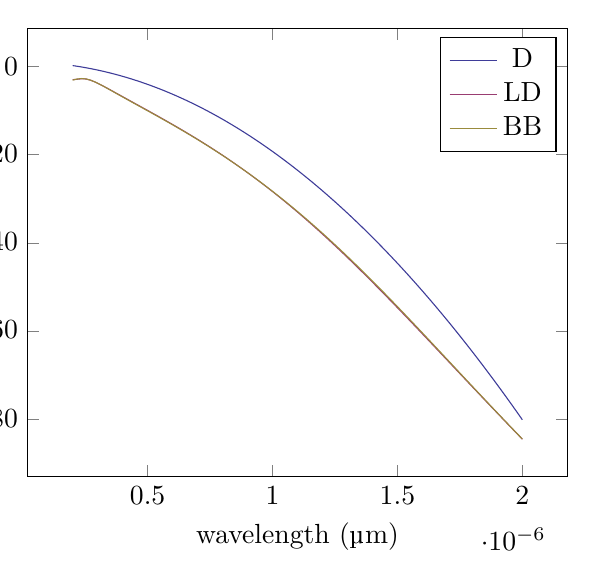
\begin{tikzpicture}[baseline,trim axis left]
\begin{axis}[xlabel=wavelength (\si{\micro\meter}),ylabel=$\epsilon'$]
\addplot[color=colora] coordinates {
(2e-07, 0.188715648446)
(2.18181818182e-07, 0.0345048789898)
(2.36363636364e-07, -0.133115411857)
(2.54545454545e-07, -0.314145196411)
(2.72727272727e-07, -0.508584444773)
(2.90909090909e-07, -0.71643312483)
(3.09090909091e-07, -0.937691202254)
(3.27272727273e-07, -1.1723586405)
(3.45454545455e-07, -1.42043540082)
(3.63636363636e-07, -1.68192144223)
(3.81818181818e-07, -1.95681672156)
(4e-07, -2.24512119339)
(4.18181818182e-07, -2.54683481011)
(4.36363636364e-07, -2.8619575219)
(4.54545454545e-07, -3.19048927671)
(4.72727272727e-07, -3.53243002028)
(4.90909090909e-07, -3.88777969614)
(5.09090909091e-07, -4.2565382456)
(5.27272727273e-07, -4.63870560776)
(5.45454545455e-07, -5.0342817195)
(5.63636363636e-07, -5.44326651549)
(5.81818181818e-07, -5.86565992818)
(6e-07, -6.30146188782)
(6.18181818182e-07, -6.75067232244)
(6.36363636364e-07, -7.21329115784)
(6.54545454545e-07, -7.68931831763)
(6.72727272727e-07, -8.17875372318)
(6.90909090909e-07, -8.68159729366)
(7.09090909091e-07, -9.19784894604)
(7.27272727273e-07, -9.72750859506)
(7.45454545455e-07, -10.2705761532)
(7.63636363636e-07, -10.8270515309)
(7.81818181818e-07, -11.3969346361)
(8e-07, -11.9802253748)
(8.18181818182e-07, -12.5769236506)
(8.36363636364e-07, -13.187029365)
(8.54545454545e-07, -13.8105424172)
(8.72727272727e-07, -14.4474627043)
(8.90909090909e-07, -15.0977901211)
(9.09090909091e-07, -15.7615245601)
(9.27272727273e-07, -16.4386659119)
(9.45454545455e-07, -17.1292140644)
(9.63636363636e-07, -17.8331689038)
(9.81818181818e-07, -18.5505303138)
(1e-06, -19.2812981758)
(1.01818181818e-06, -20.0254723692)
(1.03636363636e-06, -20.7830527712)
(1.05454545455e-06, -21.5540392566)
(1.07272727273e-06, -22.3384316981)
(1.09090909091e-06, -23.1362299661)
(1.10909090909e-06, -23.947433929)
(1.12727272727e-06, -24.7720434527)
(1.14545454545e-06, -25.6100584011)
(1.16363636364e-06, -26.4614786359)
(1.18181818182e-06, -27.3263040163)
(1.2e-06, -28.2045343997)
(1.21818181818e-06, -29.0961696409)
(1.23636363636e-06, -30.0012095928)
(1.25454545455e-06, -30.9196541059)
(1.27272727273e-06, -31.8515030285)
(1.29090909091e-06, -32.7967562068)
(1.30909090909e-06, -33.7554134847)
(1.32727272727e-06, -34.7274747039)
(1.34545454545e-06, -35.7129397038)
(1.36363636364e-06, -36.7118083218)
(1.38181818182e-06, -37.7240803929)
(1.4e-06, -38.7497557499)
(1.41818181818e-06, -39.7888342236)
(1.43636363636e-06, -40.8413156423)
(1.45454545455e-06, -41.9071998323)
(1.47272727273e-06, -42.9864866175)
(1.49090909091e-06, -44.0791758198)
(1.50909090909e-06, -45.1852672587)
(1.52727272727e-06, -46.3047607517)
(1.54545454545e-06, -47.4376561138)
(1.56363636364e-06, -48.583953158)
(1.58181818182e-06, -49.743651695)
(1.6e-06, -50.9167515335)
(1.61818181818e-06, -52.1032524796)
(1.63636363636e-06, -53.3031543375)
(1.65454545455e-06, -54.516456909)
(1.67272727273e-06, -55.7431599939)
(1.69090909091e-06, -56.9832633897)
(1.70909090909e-06, -58.2367668915)
(1.72727272727e-06, -59.5036702925)
(1.74545454545e-06, -60.7839733834)
(1.76363636364e-06, -62.0776759529)
(1.78181818182e-06, -63.3847777874)
(1.8e-06, -64.7052786712)
(1.81818181818e-06, -66.0391783861)
(1.83636363636e-06, -67.386476712)
(1.85454545455e-06, -68.7471734265)
(1.87272727273e-06, -70.1212683049)
(1.89090909091e-06, -71.5087611204)
(1.90909090909e-06, -72.9096516439)
(1.92727272727e-06, -74.3239396442)
(1.94545454545e-06, -75.7516248878)
(1.96363636364e-06, -77.1927071389)
(1.98181818182e-06, -78.6471861598)
(2e-06, -80.1150617102)
};
\addlegendentry{D}
\addplot[color=colorb] coordinates {
(2e-07, -3.00555634722)
(2.18181818182e-07, -2.9107103037)
(2.36363636364e-07, -2.78733242106)
(2.54545454545e-07, -2.86051583724)
(2.72727272727e-07, -3.14433821086)
(2.90909090909e-07, -3.56664068622)
(3.09090909091e-07, -4.0648506476)
(3.27272727273e-07, -4.60158083919)
(3.45454545455e-07, -5.15689633637)
(3.63636363636e-07, -5.72057428841)
(3.81818181818e-07, -6.28750523842)
(4e-07, -6.85526737979)
(4.18181818182e-07, -7.42287627246)
(4.36363636364e-07, -7.99013291706)
(4.54545454545e-07, -8.55727495671)
(4.72727272727e-07, -9.12478409122)
(4.90909090909e-07, -9.69327616498)
(5.09090909091e-07, -10.2634363881)
(5.27272727273e-07, -10.8359800248)
(5.45454545455e-07, -11.4116279455)
(5.63636363636e-07, -11.9910911488)
(5.81818181818e-07, -12.5750608716)
(6e-07, -13.1642022835)
(6.18181818182e-07, -13.759150541)
(6.36363636364e-07, -14.3605084239)
(6.54545454545e-07, -14.9688450534)
(6.72727272727e-07, -15.5846953495)
(6.90909090909e-07, -16.2085600003)
(7.09090909091e-07, -16.8409057772)
(7.27272727273e-07, -17.4821660827)
(7.45454545455e-07, -18.1327416461)
(7.63636363636e-07, -18.7930013089)
(7.81818181818e-07, -19.4632828539)
(8e-07, -20.1438938483)
(8.18181818182e-07, -20.8351124778)
(8.36363636364e-07, -21.5371883564)
(8.54545454545e-07, -22.2503433013)
(8.72727272727e-07, -22.9747720658)
(8.90909090909e-07, -23.7106430283)
(9.09090909091e-07, -24.4580988338)
(9.27272727273e-07, -25.2172569906)
(9.45454545455e-07, -25.988210422)
(9.63636363636e-07, -26.771027977)
(9.81818181818e-07, -27.565754903)
(1e-06, -28.3724132841)
(1.01818181818e-06, -29.1910024505)
(1.03636363636e-06, -30.0214993622)
(1.05454545455e-06, -30.8638589735)
(1.07272727273e-06, -31.7180145826)
(1.09090909091e-06, -32.5838781714)
(1.10909090909e-06, -33.4613407414)
(1.12727272727e-06, -34.3502726509)
(1.14545454545e-06, -35.2505239585)
(1.16363636364e-06, -36.1619247788)
(1.18181818182e-06, -37.084285656)
(1.2e-06, -38.0173979596)
(1.21818181818e-06, -38.9610343088)
(1.23636363636e-06, -39.9149490306)
(1.25454545455e-06, -40.8788786556)
(1.27272727273e-06, -41.8525424586)
(1.29090909091e-06, -42.835643047)
(1.30909090909e-06, -43.8278670024)
(1.32727272727e-06, -44.8288855801)
(1.34545454545e-06, -45.8383554703)
(1.36363636364e-06, -46.8559196244)
(1.38181818182e-06, -47.8812081506)
(1.4e-06, -48.9138392812)
(1.41818181818e-06, -49.9534204142)
(1.43636363636e-06, -50.9995492309)
(1.45454545455e-06, -52.0518148908)
(1.47272727273e-06, -53.1097993047)
(1.49090909091e-06, -54.1730784854)
(1.50909090909e-06, -55.2412239745)
(1.52727272727e-06, -56.3138043444)
(1.54545454545e-06, -57.3903867724)
(1.56363636364e-06, -58.4705386825)
(1.58181818182e-06, -59.5538294509)
(1.6e-06, -60.6398321691)
(1.61818181818e-06, -61.7281254578)
(1.63636363636e-06, -62.8182953241)
(1.65454545455e-06, -63.9099370528)
(1.67272727273e-06, -65.0026571227)
(1.69090909091e-06, -66.0960751358)
(1.70909090909e-06, -67.1898257504)
(1.72727272727e-06, -68.2835606025)
(1.74545454545e-06, -69.376950206)
(1.76363636364e-06, -70.4696858152)
(1.78181818182e-06, -71.5614812377)
(1.8e-06, -72.6520745829)
(1.81818181818e-06, -73.7412299312)
(1.83636363636e-06, -74.8287389105)
(1.85454545455e-06, -75.9144221659)
(1.87272727273e-06, -76.9981307088)
(1.89090909091e-06, -78.0797471326)
(1.90909090909e-06, -79.1591866831)
(1.92727272727e-06, -80.2363981725)
(1.94545454545e-06, -81.3113647266)
(1.96363636364e-06, -82.3841043578)
(1.98181818182e-06, -83.4546703557)
(2e-06, -84.5231514902)
};
\addlegendentry{LD}
\addplot[color=colorc] coordinates {
(2e-07, -3.10392533429)
(2.18181818182e-07, -2.85707922232)
(2.36363636364e-07, -2.74856891561)
(2.54545454545e-07, -2.85053966998)
(2.72727272727e-07, -3.13958171118)
(2.90909090909e-07, -3.56210991213)
(3.09090909091e-07, -4.06747737021)
(3.27272727273e-07, -4.618333628)
(3.45454545455e-07, -5.19062390903)
(3.63636363636e-07, -5.77039246883)
(3.81818181818e-07, -6.35041506783)
(4e-07, -6.9275845299)
(4.18181818182e-07, -7.5011311596)
(4.36363636364e-07, -8.07150385215)
(4.54545454545e-07, -8.63970846817)
(4.72727272727e-07, -9.20693960798)
(4.90909090909e-07, -9.7743907698)
(5.09090909091e-07, -10.3431679546)
(5.27272727273e-07, -10.9142597857)
(5.45454545455e-07, -11.4885372525)
(5.63636363636e-07, -12.0667659389)
(5.81818181818e-07, -12.6496229094)
(6e-07, -13.2377134488)
(6.18181818182e-07, -13.8315857065)
(6.36363636364e-07, -14.4317425708)
(6.54545454545e-07, -15.0386507855)
(6.72727272727e-07, -15.6527476337)
(6.90909090909e-07, -16.2744456215)
(7.09090909091e-07, -16.9041355982)
(7.27272727273e-07, -17.5421887013)
(7.45454545455e-07, -18.1889574537)
(7.63636363636e-07, -18.8447762689)
(7.81818181818e-07, -19.5099615648)
(8e-07, -20.1848116324)
(8.18181818182e-07, -20.8696063664)
(8.36363636364e-07, -21.5646069315)
(8.54545454545e-07, -22.2700554132)
(8.72727272727e-07, -22.9861744845)
(8.90909090909e-07, -23.7131671072)
(9.09090909091e-07, -24.451216275)
(9.27272727273e-07, -25.2004848012)
(9.45454545455e-07, -25.9611151502)
(9.63636363636e-07, -26.7332293071)
(9.81818181818e-07, -27.5169286819)
(1e-06, -28.3122940406)
(1.01818181818e-06, -29.1193854593)
(1.03636363636e-06, -29.9382422952)
(1.05454545455e-06, -30.7688831704)
(1.07272727273e-06, -31.6113059662)
(1.09090909091e-06, -32.4654878237)
(1.10909090909e-06, -33.3313851506)
(1.12727272727e-06, -34.208933634)
(1.14545454545e-06, -35.0980482584)
(1.16363636364e-06, -35.998623332)
(1.18181818182e-06, -36.9105325222)
(1.2e-06, -37.8336289055)
(1.21818181818e-06, -38.7677457034)
(1.23636363636e-06, -39.7126936943)
(1.25454545455e-06, -40.6682653335)
(1.27272727273e-06, -41.6342322384)
(1.29090909091e-06, -42.6103460395)
(1.30909090909e-06, -43.5963386152)
(1.32727272727e-06, -44.5919223796)
(1.34545454545e-06, -45.5967906325)
(1.36363636364e-06, -46.6106186386)
(1.38181818182e-06, -47.633061493)
(1.4e-06, -48.663758643)
(1.41818181818e-06, -49.7023319471)
(1.43636363636e-06, -50.7483871085)
(1.45454545455e-06, -51.8015145647)
(1.47272727273e-06, -52.8612904945)
(1.49090909091e-06, -53.927277949)
(1.50909090909e-06, -54.999028111)
(1.52727272727e-06, -56.0760816892)
(1.54545454545e-06, -57.1579704482)
(1.56363636364e-06, -58.2442188796)
(1.58181818182e-06, -59.334346011)
(1.6e-06, -60.4278673544)
(1.61818181818e-06, -61.5242969886)
(1.63636363636e-06, -62.6231497716)
(1.65454545455e-06, -63.723943674)
(1.67272727273e-06, -64.826202224)
(1.69090909091e-06, -65.9294570512)
(1.70909090909e-06, -67.033250514)
(1.72727272727e-06, -68.1371383936)
(1.74545454545e-06, -69.2406926342)
(1.76363636364e-06, -70.3435041082)
(1.78181818182e-06, -71.4451853821)
(1.8e-06, -72.5453734567)
(1.81818181818e-06, -73.6437324568)
(1.83636363636e-06, -74.7399562398)
(1.85454545455e-06, -75.8337708963)
(1.87272727273e-06, -76.9249371137)
(1.89090909091e-06, -78.0132523743)
(1.90909090909e-06, -79.0985529611)
(1.92727272727e-06, -80.1807157449)
(1.94545454545e-06, -81.2596597293)
(1.96363636364e-06, -82.3353473319)
(1.98181818182e-06, -83.4077853836)
(2e-06, -84.4770258306)
};
\addlegendentry{BB}
\end{axis}
\end{tikzpicture}%
\\
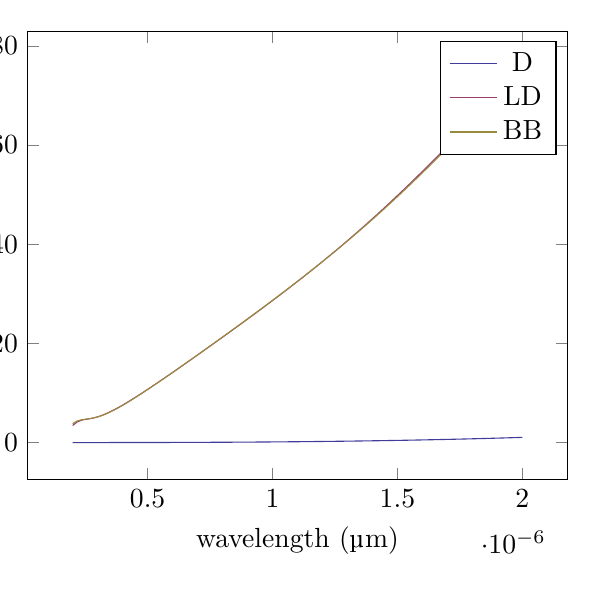
\begin{tikzpicture}[baseline,trim axis left]
\begin{axis}[xlabel=wavelength (\si{\micro\meter}),ylabel=$\epsilon''$]
\addplot[color=colora] coordinates {
(2e-07, 0.00104695197986)
(2.18181818182e-07, 0.00135922798535)
(2.36363636364e-07, 0.00172813822703)
(2.54545454545e-07, 0.00215840215422)
(2.72727272727e-07, 0.00265473919932)
(2.90909090909e-07, 0.0032218687766)
(3.09090909091e-07, 0.00386451028078)
(3.27272727273e-07, 0.00458738308584)
(3.45454545455e-07, 0.00539520654367)
(3.63636363636e-07, 0.00629269998275)
(3.81818181818e-07, 0.00728458270691)
(4e-07, 0.00837557399396)
(4.18181818182e-07, 0.00957039309448)
(4.36363636364e-07, 0.0108737592304)
(4.54545454545e-07, 0.0122903915939)
(4.72727272727e-07, 0.0138250093458)
(4.90909090909e-07, 0.0154823316146)
(5.09090909091e-07, 0.0172670774949)
(5.27272727273e-07, 0.0191839660464)
(5.45454545455e-07, 0.0212377162923)
(5.63636363636e-07, 0.023433047218)
(5.81818181818e-07, 0.0257746777702)
(6e-07, 0.0282673268553)
(6.18181818182e-07, 0.0309157133378)
(6.36363636364e-07, 0.0337245560397)
(6.54545454545e-07, 0.0366985737388)
(6.72727272727e-07, 0.0398424851672)
(6.90909090909e-07, 0.0431610090104)
(7.09090909091e-07, 0.0466588639059)
(7.27272727273e-07, 0.0503407684417)
(7.45454545455e-07, 0.0542114411551)
(7.63636363636e-07, 0.0582756005318)
(7.81818181818e-07, 0.0625379650037)
(8e-07, 0.0670032529487)
(8.18181818182e-07, 0.0716761826883)
(8.36363636364e-07, 0.0765614724874)
(8.54545454545e-07, 0.081663840552)
(8.72727272727e-07, 0.0869880050286)
(8.90909090909e-07, 0.0925386840025)
(9.09090909091e-07, 0.0983205954969)
(9.27272727273e-07, 0.104338457471)
(9.45454545455e-07, 0.11059698782)
(9.63636363636e-07, 0.11710090437)
(9.81818181818e-07, 0.123854924885)
(1e-06, 0.130863767054)
(1.01818181818e-06, 0.1381321485)
(1.03636363636e-06, 0.145664786772)
(1.05454545455e-06, 0.15346639935)
(1.07272727273e-06, 0.161541703635)
(1.09090909091e-06, 0.169895416957)
(1.10909090909e-06, 0.178532256567)
(1.12727272727e-06, 0.187456939638)
(1.14545454545e-06, 0.196674183265)
(1.16363636364e-06, 0.206188704462)
(1.18181818182e-06, 0.216005220161)
(1.2e-06, 0.226128447211)
(1.21818181818e-06, 0.236563102376)
(1.23636363636e-06, 0.247313902336)
(1.25454545455e-06, 0.258385563683)
(1.27272727273e-06, 0.269782802919)
(1.29090909091e-06, 0.281510336459)
(1.30909090909e-06, 0.293572880626)
(1.32727272727e-06, 0.305975151651)
(1.34545454545e-06, 0.318721865671)
(1.36363636364e-06, 0.331817738729)
(1.38181818182e-06, 0.345267486771)
(1.4e-06, 0.359075825647)
(1.41818181818e-06, 0.373247471107)
(1.43636363636e-06, 0.387787138801)
(1.45454545455e-06, 0.402699544279)
(1.47272727273e-06, 0.417989402987)
(1.49090909091e-06, 0.433661430268)
(1.50909090909e-06, 0.44972034136)
(1.52727272727e-06, 0.466170851394)
(1.54545454545e-06, 0.483017675393)
(1.56363636364e-06, 0.500265528272)
(1.58181818182e-06, 0.517919124834)
(1.6e-06, 0.535983179773)
(1.61818181818e-06, 0.554462407666)
(1.63636363636e-06, 0.57336152298)
(1.65454545455e-06, 0.592685240065)
(1.67272727273e-06, 0.612438273152)
(1.69090909091e-06, 0.632625336357)
(1.70909090909e-06, 0.653251143675)
(1.72727272727e-06, 0.67432040898)
(1.74545454545e-06, 0.695837846025)
(1.76363636364e-06, 0.71780816844)
(1.78181818182e-06, 0.740236089728)
(1.8e-06, 0.763126323269)
(1.81818181818e-06, 0.786483582313)
(1.83636363636e-06, 0.810312579985)
(1.85454545455e-06, 0.834618029277)
(1.87272727273e-06, 0.859404643051)
(1.89090909091e-06, 0.884677134038)
(1.90909090909e-06, 0.910440214833)
(1.92727272727e-06, 0.936698597897)
(1.94545454545e-06, 0.963456995556)
(1.96363636364e-06, 0.990720119996)
(1.98181818182e-06, 1.01849268327)
(2e-06, 1.04677939727)
};
\addlegendentry{D}
\addplot[color=colorb] coordinates {
(2e-07, 3.44515696201)
(2.18181818182e-07, 4.15663052382)
(2.36363636364e-07, 4.5300281151)
(2.54545454545e-07, 4.69901849727)
(2.72727272727e-07, 4.84486155278)
(2.90909090909e-07, 5.05157224971)
(3.09090909091e-07, 5.33518515803)
(3.27272727273e-07, 5.68762661117)
(3.45454545455e-07, 6.09621134718)
(3.63636363636e-07, 6.54948526924)
(3.81818181818e-07, 7.03829516503)
(4e-07, 7.55555552391)
(4.18181818182e-07, 8.09579021866)
(4.36363636364e-07, 8.65472807999)
(4.54545454545e-07, 9.22899720381)
(4.72727272727e-07, 9.81590424421)
(4.90909090909e-07, 10.4132763867)
(5.09090909091e-07, 11.0193473171)
(5.27272727273e-07, 11.6326736817)
(5.45454545455e-07, 12.2520727633)
(5.63636363636e-07, 12.8765750955)
(5.81818181818e-07, 13.5053877697)
(6e-07, 14.1378655349)
(6.18181818182e-07, 14.7734876858)
(6.36363636364e-07, 15.4118393266)
(6.54545454545e-07, 16.0525960028)
(6.72727272727e-07, 16.6955109656)
(6.90909090909e-07, 17.340404521)
(7.09090909091e-07, 17.9871550538)
(7.27272727273e-07, 18.6356914081)
(7.45454545455e-07, 19.285986379)
(7.63636363636e-07, 19.9380511184)
(7.81818181818e-07, 20.5919303006)
(8e-07, 21.24769792)
(8.18181818182e-07, 21.9054536176)
(8.36363636364e-07, 22.5653194518)
(8.54545454545e-07, 23.227437041)
(8.72727272727e-07, 23.8919650215)
(8.90909090909e-07, 24.5590767672)
(9.09090909091e-07, 25.2289583334)
(9.27272727273e-07, 25.9018065853)
(9.45454545455e-07, 26.5778274831)
(9.63636363636e-07, 27.2572344974)
(9.81818181818e-07, 27.9402471317)
(1e-06, 28.6270895349)
(1.01818181818e-06, 29.3179891859)
(1.03636363636e-06, 30.0131756375)
(1.05454545455e-06, 30.7128793067)
(1.07272727273e-06, 31.4173303023)
(1.09090909091e-06, 32.1267572801)
(1.10909090909e-06, 32.8413863197)
(1.12727272727e-06, 33.5614398148)
(1.14545454545e-06, 34.2871353747)
(1.16363636364e-06, 35.0186847309)
(1.18181818182e-06, 35.7562926464)
(1.2e-06, 36.5001558259)
(1.21818181818e-06, 37.2504618252)
(1.23636363636e-06, 38.007387959)
(1.25454545455e-06, 38.7711002079)
(1.27272727273e-06, 39.5417521248)
(1.29090909091e-06, 40.3194837426)
(1.30909090909e-06, 41.1044204852)
(1.32727272727e-06, 41.8966720854)
(1.34545454545e-06, 42.6963315119)
(1.36363636364e-06, 43.5034739119)
(1.38181818182e-06, 44.3181555707)
(1.4e-06, 45.1404128974)
(1.41818181818e-06, 45.9702614396)
(1.43636363636e-06, 46.8076949357)
(1.45454545455e-06, 47.65268441)
(1.47272727273e-06, 48.5051773191)
(1.49090909091e-06, 49.3650967572)
(1.50909090909e-06, 50.2323407274)
(1.52727272727e-06, 51.106781488)
(1.54545454545e-06, 51.9882649825)
(1.56363636364e-06, 52.8766103601)
(1.58181818182e-06, 53.7716095968)
(1.6e-06, 54.6730272244)
(1.61818181818e-06, 55.5806001746)
(1.63636363636e-06, 56.4940377473)
(1.65454545455e-06, 57.4130217082)
(1.67272727273e-06, 58.3372065232)
(1.69090909091e-06, 59.2662197343)
(1.70909090909e-06, 60.1996624818)
(1.72727272727e-06, 61.1371101764)
(1.74545454545e-06, 62.0781133229)
(1.76363636364e-06, 63.0221984973)
(1.78181818182e-06, 63.9688694766)
(1.8e-06, 64.9176085191)
(1.81818181818e-06, 65.8678777929)
(1.83636363636e-06, 66.8191209471)
(1.85454545455e-06, 67.7707648199)
(1.87272727273e-06, 68.7222212745)
(1.89090909091e-06, 69.6728891554)
(1.90909090909e-06, 70.6221563524)
(1.92727272727e-06, 71.5694019612)
(1.94545454545e-06, 72.5139985259)
(1.96363636364e-06, 73.4553143506)
(1.98181818182e-06, 74.3927158622)
(2e-06, 75.3255700097)
};
\addlegendentry{LD}
\addplot[color=colorc] coordinates {
(2e-07, 3.824872901)
(2.18181818182e-07, 4.35874141755)
(2.36363636364e-07, 4.61075624872)
(2.54545454545e-07, 4.74263089456)
(2.72727272727e-07, 4.87107627306)
(2.90909090909e-07, 5.05555574576)
(3.09090909091e-07, 5.31572317839)
(3.27272727273e-07, 5.65009939142)
(3.45454545455e-07, 6.04850401392)
(3.63636363636e-07, 6.49872898945)
(3.81818181818e-07, 6.98953159385)
(4e-07, 7.51164813756)
(4.18181818182e-07, 8.05787844342)
(4.36363636364e-07, 8.62280502985)
(4.54545454545e-07, 9.2024194281)
(4.72727272727e-07, 9.79377192917)
(4.90909090909e-07, 10.3946841593)
(5.09090909091e-07, 11.0035292971)
(5.27272727273e-07, 11.6190712703)
(5.45454545455e-07, 12.2403506753)
(5.63636363636e-07, 12.8666056576)
(5.81818181818e-07, 13.4972180192)
(6e-07, 14.131677004)
(6.18181818182e-07, 14.7695551931)
(6.36363636364e-07, 15.4104925202)
(6.54545454545e-07, 16.0541856216)
(6.72727272727e-07, 16.7003806164)
(6.90909090909e-07, 17.3488680431)
(7.09090909091e-07, 17.9994791151)
(7.27272727273e-07, 18.6520827608)
(7.45454545455e-07, 19.3065831152)
(7.63636363636e-07, 19.9629172648)
(7.81818181818e-07, 20.6210531298)
(8e-07, 21.2809874272)
(8.18181818182e-07, 21.9427436858)
(8.36363636364e-07, 22.6063703052)
(8.54545454545e-07, 23.2719386606)
(8.72727272727e-07, 23.9395412588)
(8.90909090909e-07, 24.6092899506)
(9.09090909091e-07, 25.2813142077)
(9.27272727273e-07, 25.9557594657)
(9.45454545455e-07, 26.6327855354)
(9.63636363636e-07, 27.3125650835)
(9.81818181818e-07, 27.9952821789)
(1e-06, 28.6811309019)
(1.01818181818e-06, 29.3703140112)
(1.03636363636e-06, 30.0630416627)
(1.05454545455e-06, 30.7595301732)
(1.07272727273e-06, 31.4600008236)
(1.09090909091e-06, 32.1646786915)
(1.10909090909e-06, 32.8737915092)
(1.12727272727e-06, 33.5875685376)
(1.14545454545e-06, 34.3062394493)
(1.16363636364e-06, 35.0300332162)
(1.18181818182e-06, 35.7591769921)
(1.2e-06, 36.4938949881)
(1.21818181818e-06, 37.2344075374)
(1.23636363636e-06, 37.9809291044)
(1.25454545455e-06, 38.7336683755)
(1.27272727273e-06, 39.4928261903)
(1.29090909091e-06, 40.2585945274)
(1.30909090909e-06, 41.0311552403)
(1.32727272727e-06, 41.8106787648)
(1.34545454545e-06, 42.5973227956)
(1.36363636364e-06, 43.3912311902)
(1.38181818182e-06, 44.1925315652)
(1.4e-06, 45.0013354568)
(1.41818181818e-06, 45.8177358567)
(1.43636363636e-06, 46.6418060531)
(1.45454545455e-06, 47.4735982027)
(1.47272727273e-06, 48.3131419097)
(1.49090909091e-06, 49.1604428201)
(1.50909090909e-06, 50.015481243)
(1.52727272727e-06, 50.8782108121)
(1.54545454545e-06, 51.7485572008)
(1.56363636364e-06, 52.6264169054)
(1.58181818182e-06, 53.5116561122)
(1.6e-06, 54.4041096656)
(1.61818181818e-06, 55.3035801533)
(1.63636363636e-06, 56.2098371266)
(1.65454545455e-06, 57.1226164735)
(1.67272727273e-06, 58.0416199613)
(1.69090909091e-06, 58.9665149655)
(1.70909090909e-06, 59.8969344017)
(1.72727272727e-06, 60.8324768744)
(1.74545454545e-06, 61.7727070553)
(1.76363636364e-06, 62.7171563035)
(1.78181818182e-06, 63.6653235354)
(1.8e-06, 64.6166763501)
(1.81818181818e-06, 65.5706524145)
(1.83636363636e-06, 66.526661107)
(1.85454545455e-06, 67.4840854162)
(1.87272727273e-06, 68.4422840885)
(1.89090909091e-06, 69.4005940121)
(1.90909090909e-06, 70.3583328248)
(1.92727272727e-06, 71.314801726)
(1.94545454545e-06, 72.2692884723)
(1.96363636364e-06, 73.2210705325)
(1.98181818182e-06, 74.1694183735)
(2e-06, 75.1135988483)
};
\addlegendentry{BB}
\end{axis}
\end{tikzpicture}%
\\
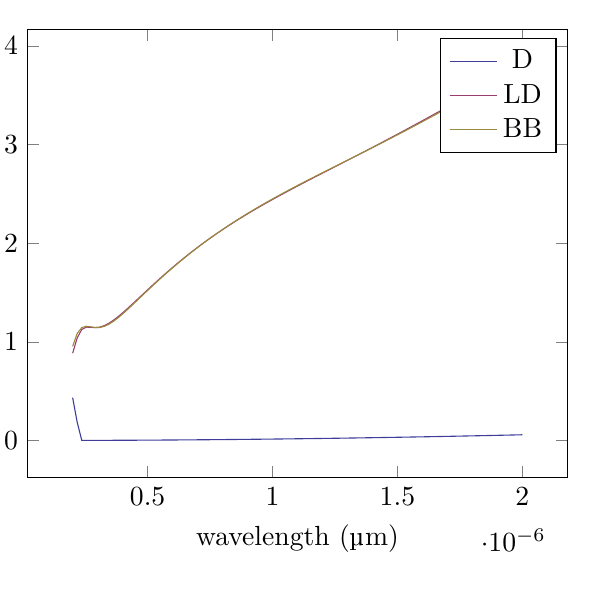
\begin{tikzpicture}[baseline,trim axis left]
\begin{axis}[xlabel=wavelength (\si{\micro\meter}),ylabel=$n'$]
\addplot[color=colora] coordinates {
(2e-07, 0.434415815203)
(2.18181818182e-07, 0.185790902883)
(2.36363636364e-07, 0.0023682370023)
(2.54545454545e-07, 0.00192546042072)
(2.72727272727e-07, 0.00186126774502)
(2.90909090909e-07, 0.00190321970595)
(3.09090909091e-07, 0.00199541681954)
(3.27272727273e-07, 0.00211838034276)
(3.45454545455e-07, 0.00226342731562)
(3.63636363636e-07, 0.00242607050081)
(3.81818181818e-07, 0.00260374743479)
(4e-07, 0.00279488494186)
(4.18181818182e-07, 0.00299846252626)
(4.36363636364e-07, 0.003213788863)
(4.54545454545e-07, 0.00344037889336)
(4.72727272727e-07, 0.0036778822671)
(4.90909090909e-07, 0.00392603968394)
(5.09090909091e-07, 0.00418465519621)
(5.27272727273e-07, 0.00445357804513)
(5.45454545455e-07, 0.0047326904061)
(5.63636363636e-07, 0.00502189891275)
(5.81818181818e-07, 0.00532112866703)
(6e-07, 0.00563031892304)
(6.18181818182e-07, 0.00594941992434)
(6.36363636364e-07, 0.00627839054999)
(6.54545454545e-07, 0.00661719653839)
(6.72727272727e-07, 0.00696580912994)
(6.90909090909e-07, 0.00732420401817)
(7.09090909091e-07, 0.00769236053075)
(7.27272727273e-07, 0.00807026098309)
(7.45454545455e-07, 0.00845789016464)
(7.63636363636e-07, 0.0088552349268)
(7.81818181818e-07, 0.00926228384963)
(8e-07, 0.00967902697059)
(8.18181818182e-07, 0.0101054555626)
(8.36363636364e-07, 0.0105415619508)
(8.54545454545e-07, 0.0109873393608)
(8.72727272727e-07, 0.0114427817917)
(8.90909090909e-07, 0.0119078839107)
(9.09090909091e-07, 0.0123826409631)
(9.27272727273e-07, 0.012867048697)
(9.45454545455e-07, 0.0133611032997)
(9.63636363636e-07, 0.0138648013418)
(9.81818181818e-07, 0.0143781397315)
(1e-06, 0.0149011156735)
(1.01818181818e-06, 0.0154337266349)
(1.03636363636e-06, 0.0159759703148)
(1.05454545455e-06, 0.0165278446181)
(1.07272727273e-06, 0.0170893476333)
(1.09090909091e-06, 0.0176604776122)
(1.10909090909e-06, 0.0182412329526)
(1.12727272727e-06, 0.0188316121833)
(1.14545454545e-06, 0.0194316139506)
(1.16363636364e-06, 0.0200412370063)
(1.18181818182e-06, 0.0206604801973)
(1.2e-06, 0.0212893424565)
(1.21818181818e-06, 0.0219278227944)
(1.23636363636e-06, 0.0225759202918)
(1.25454545455e-06, 0.0232336340932)
(1.27272727273e-06, 0.023900963401)
(1.29090909091e-06, 0.0245779074702)
(1.30909090909e-06, 0.0252644656039)
(1.32727272727e-06, 0.0259606371489)
(1.34545454545e-06, 0.0266664214918)
(1.36363636364e-06, 0.0273818180559)
(1.38181818182e-06, 0.0281068262978)
(1.4e-06, 0.0288414457048)
(1.41818181818e-06, 0.0295856757922)
(1.43636363636e-06, 0.0303395161011)
(1.45454545455e-06, 0.0311029661964)
(1.47272727273e-06, 0.0318760256645)
(1.49090909091e-06, 0.0326586941123)
(1.50909090909e-06, 0.0334509711647)
(1.52727272727e-06, 0.0342528564642)
(1.54545454545e-06, 0.0350643496685)
(1.56363636364e-06, 0.0358854504501)
(1.58181818182e-06, 0.0367161584948)
(1.6e-06, 0.0375564735009)
(1.61818181818e-06, 0.0384063951781)
(1.63636363636e-06, 0.0392659232467)
(1.65454545455e-06, 0.0401350574369)
(1.67272727273e-06, 0.0410137974878)
(1.69090909091e-06, 0.0419021431473)
(1.70909090909e-06, 0.0428000941708)
(1.72727272727e-06, 0.0437076503209)
(1.74545454545e-06, 0.0446248113672)
(1.76363636364e-06, 0.0455515770851)
(1.78181818182e-06, 0.0464879472563)
(1.8e-06, 0.0474339216675)
(1.81818181818e-06, 0.0483895001103)
(1.83636363636e-06, 0.0493546823811)
(1.85454545455e-06, 0.0503294682805)
(1.87272727273e-06, 0.051313857613)
(1.89090909091e-06, 0.0523078501868)
(1.90909090909e-06, 0.0533114458135)
(1.92727272727e-06, 0.0543246443077)
(1.94545454545e-06, 0.0553474454871)
(1.96363636364e-06, 0.056379849172)
(1.98181818182e-06, 0.0574218551851)
(2e-06, 0.0584734633513)
};
\addlegendentry{D}
\addplot[color=colorb] coordinates {
(2e-07, 0.884976317216)
(2.18181818182e-07, 1.04012425539)
(2.36363636364e-07, 1.12506387688)
(2.54545454545e-07, 1.14906384853)
(2.72727272727e-07, 1.1470471089)
(2.90909090909e-07, 1.14393035039)
(3.09090909091e-07, 1.14943464701)
(3.27272727273e-07, 1.16499025367)
(3.45454545455e-07, 1.18910156265)
(3.63636363636e-07, 1.21972202182)
(3.81818181818e-07, 1.25503031055)
(4e-07, 1.29358950663)
(4.18181818182e-07, 1.33431431673)
(4.36363636364e-07, 1.37639734356)
(4.54545454545e-07, 1.41924004629)
(4.72727272727e-07, 1.46239837757)
(4.90909090909e-07, 1.50554244636)
(5.09090909091e-07, 1.54842718933)
(5.27272727273e-07, 1.59087111784)
(5.45454545455e-07, 1.63274084406)
(5.63636363636e-07, 1.67393971712)
(5.81818181818e-07, 1.71439939103)
(6e-07, 1.754073499)
(6.18181818182e-07, 1.79293285655)
(6.36363636364e-07, 1.83096178578)
(6.54545454545e-07, 1.86815527121)
(6.72727272727e-07, 1.90451673907)
(6.90909090909e-07, 1.94005630872)
(7.09090909091e-07, 1.97478940544)
(7.27272727273e-07, 2.00873565184)
(7.45454545455e-07, 2.04191797646)
(7.63636363636e-07, 2.07436189243)
(7.81818181818e-07, 2.10609491055)
(8e-07, 2.13714605922)
(8.18181818182e-07, 2.16754548963)
(8.36363636364e-07, 2.1973241495)
(8.54545454545e-07, 2.22651351218)
(8.72727272727e-07, 2.25514535045)
(8.90909090909e-07, 2.28325154679)
(9.09090909091e-07, 2.31086393334)
(9.27272727273e-07, 2.33801415611)
(9.45454545455e-07, 2.36473355913)
(9.63636363636e-07, 2.391053085)
(9.81818181818e-07, 2.41700318877)
(1e-06, 2.44261376311)
(1.01818181818e-06, 2.4679140725)
(1.03636363636e-06, 2.49293269508)
(1.05454545455e-06, 2.51769747072)
(1.07272727273e-06, 2.54223545433)
(1.09090909091e-06, 2.56657287344)
(1.10909090909e-06, 2.59073508944)
(1.12727272727e-06, 2.61474656166)
(1.14545454545e-06, 2.63863081413)
(1.16363636364e-06, 2.66241040424)
(1.18181818182e-06, 2.68610689334)
(1.2e-06, 2.70974081872)
(1.21818181818e-06, 2.73333166703)
(1.23636363636e-06, 2.75689784874)
(1.25454545455e-06, 2.78045667379)
(1.27272727273e-06, 2.80402432811)
(1.29090909091e-06, 2.82761585121)
(1.30909090909e-06, 2.85124511465)
(1.32727272727e-06, 2.87492480151)
(1.34545454545e-06, 2.89866638695)
(1.36363636364e-06, 2.92248011983)
(1.38181818182e-06, 2.94637500554)
(1.4e-06, 2.97035879021)
(1.41818181818e-06, 2.99443794638)
(1.43636363636e-06, 3.01861766029)
(1.45454545455e-06, 3.04290182093)
(1.47272727273e-06, 3.06729301122)
(1.49090909091e-06, 3.09179250119)
(1.50909090909e-06, 3.11640024369)
(1.52727272727e-06, 3.14111487266)
(1.54545454545e-06, 3.16593370419)
(1.56363636364e-06, 3.19085274068)
(1.58181818182e-06, 3.21586667821)
(1.6e-06, 3.24096891738)
(1.61818181818e-06, 3.2661515779)
(1.63636363636e-06, 3.2914055169)
(1.65454545455e-06, 3.31672035146)
(1.67272727273e-06, 3.3420844852)
(1.69090909091e-06, 3.36748513929)
(1.70909090909e-06, 3.3929083879)
(1.72727272727e-06, 3.41833919818)
(1.74545454545e-06, 3.44376147482)
(1.76363636364e-06, 3.46915810925)
(1.78181818182e-06, 3.49451103339)
(1.8e-06, 3.51980127793)
(1.81818181818e-06, 3.54500903504)
(1.83636363636e-06, 3.57011372532)
(1.85454545455e-06, 3.59509406887)
(1.87272727273e-06, 3.61992816021)
(1.89090909091e-06, 3.64459354668)
(1.90909090909e-06, 3.66906731024)
(1.92727272727e-06, 3.69332615198)
(1.94545454545e-06, 3.71734647927)
(1.96363636364e-06, 3.74110449486)
(1.98181818182e-06, 3.76457628761)
(2e-06, 3.78773792428)
};
\addlegendentry{LD}
\addplot[color=colorc] coordinates {
(2e-07, 0.954443652846)
(2.18181818182e-07, 1.08503297257)
(2.36363636364e-07, 1.14439304839)
(2.54545454545e-07, 1.15819362966)
(2.72727272727e-07, 1.15230628003)
(2.90909090909e-07, 1.145060673)
(3.09090909091e-07, 1.14584004951)
(3.27272727273e-07, 1.1573906515)
(3.45454545455e-07, 1.1789311573)
(3.63636363636e-07, 1.20839966221)
(3.81818181818e-07, 1.24361796732)
(4e-07, 1.28274006978)
(4.18181818182e-07, 1.32434725398)
(4.36363636364e-07, 1.36740449912)
(4.54545454545e-07, 1.41117931149)
(4.72727272727e-07, 1.45516299819)
(4.90909090909e-07, 1.49900667102)
(5.09090909091e-07, 1.54247320912)
(5.27272727273e-07, 1.58540275217)
(5.45454545455e-07, 1.62768852366)
(5.63636363636e-07, 1.6692602223)
(5.81818181818e-07, 1.71007271672)
(6e-07, 1.75009841807)
(6.18181818182e-07, 1.7893221547)
(6.36363636364e-07, 1.82773773112)
(6.54545454545e-07, 1.8653456098)
(6.72727272727e-07, 1.90215133587)
(6.90909090909e-07, 1.93816444973)
(7.09090909091e-07, 1.97339771876)
(7.27272727273e-07, 2.00786657692)
(7.45454545455e-07, 2.04158869987)
(7.63636363636e-07, 2.07458366919)
(7.81818181818e-07, 2.1068726958)
(8e-07, 2.13847838395)
(8.18181818182e-07, 2.16942452408)
(8.36363636364e-07, 2.19973590726)
(8.54545454545e-07, 2.22943815674)
(8.72727272727e-07, 2.25855757387)
(8.90909090909e-07, 2.28712099662)
(9.09090909091e-07, 2.31515566934)
(9.27272727273e-07, 2.34268912311)
(9.45454545455e-07, 2.36974906561)
(9.63636363636e-07, 2.39636328015)
(9.81818181818e-07, 2.42255953292)
(1e-06, 2.44836548801)
(1.01818181818e-06, 2.47380862945)
(1.03636363636e-06, 2.49891618959)
(1.05454545455e-06, 2.52371508329)
(1.07272727273e-06, 2.54823184715)
(1.09090909091e-06, 2.57249258326)
(1.10909090909e-06, 2.59652290679)
(1.12727272727e-06, 2.620347897)
(1.14545454545e-06, 2.64399205098)
(1.16363636364e-06, 2.66747923975)
(1.18181818182e-06, 2.69083266619)
(1.2e-06, 2.71407482448)
(1.21818181818e-06, 2.73722745641)
(1.23636363636e-06, 2.76031152825)
(1.25454545455e-06, 2.78334717058)
(1.27272727273e-06, 2.80635365379)
(1.29090909091e-06, 2.82934934695)
(1.30909090909e-06, 2.85235167967)
(1.32727272727e-06, 2.8753771038)
(1.34545454545e-06, 2.89844105474)
(1.36363636364e-06, 2.92155791224)
(1.38181818182e-06, 2.94474096166)
(1.4e-06, 2.96800235501)
(1.41818181818e-06, 2.99135307044)
(1.43636363636e-06, 3.01480287341)
(1.45454545455e-06, 3.03836027765)
(1.47272727273e-06, 3.06203250689)
(1.49090909091e-06, 3.08582545736)
(1.50909090909e-06, 3.10974366171)
(1.52727272727e-06, 3.13379025462)
(1.54545454545e-06, 3.15796694053)
(1.56363636364e-06, 3.18227396409)
(1.58181818182e-06, 3.20671008375)
(1.6e-06, 3.23127254902)
(1.61818181818e-06, 3.25595708212)
(1.63636363636e-06, 3.28075786434)
(1.65454545455e-06, 3.30566752795)
(1.67272727273e-06, 3.33067715404)
(1.69090909091e-06, 3.35577627697)
(1.70909090909e-06, 3.38095289581)
(1.72727272727e-06, 3.40619349342)
(1.74545454545e-06, 3.43148306345)
(1.76363636364e-06, 3.45680514574)
(1.78181818182e-06, 3.48214187029)
(1.8e-06, 3.50747401012)
(1.81818181818e-06, 3.53278104302)
(1.83636363636e-06, 3.55804122228)
(1.85454545455e-06, 3.58323165615)
(1.87272727273e-06, 3.608328396)
(1.89090909091e-06, 3.63330653262)
(1.90909090909e-06, 3.65814030033)
(1.92727272727e-06, 3.68280318824)
(1.94545454545e-06, 3.70726805798)
(1.96363636364e-06, 3.73150726718)
(1.98181818182e-06, 3.75549279761)
(2e-06, 3.77919638719)
};
\addlegendentry{BB}
\end{axis}
\end{tikzpicture}%
\\
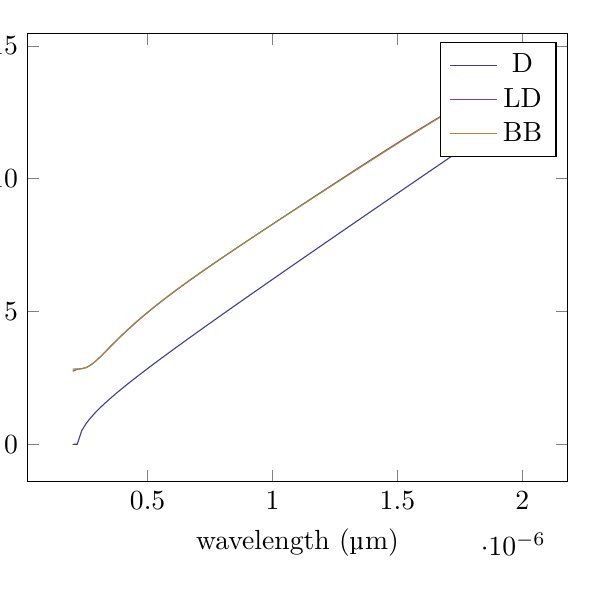
\begin{tikzpicture}[baseline,trim axis left]
\begin{axis}[xlabel=wavelength (\si{\micro\meter}),ylabel=$n''$]
\addplot[color=colora] coordinates {
(2e-07, 0.00170414340045)
(2.18181818182e-07, 0.00517312371437)
(2.36363636364e-07, 0.515986473474)
(2.54545454545e-07, 0.792652387631)
(2.72727272727e-07, 1.00855134633)
(2.90909090909e-07, 1.19702693961)
(3.09090909091e-07, 1.36944892854)
(3.27272727273e-07, 1.53124989994)
(3.45454545455e-07, 1.68549133722)
(3.63636363636e-07, 1.83408142025)
(3.81818181818e-07, 1.97829396251)
(4e-07, 2.11902289028)
(4.18181818182e-07, 2.25691993695)
(4.36363636364e-07, 2.3924748067)
(4.54545454545e-07, 2.52606457278)
(4.72727272727e-07, 2.65798553311)
(4.90909090909e-07, 2.78847453276)
(5.09090909091e-07, 2.91772368703)
(5.27272727273e-07, 3.04589081949)
(5.45454545455e-07, 3.17310703187)
(5.63636363636e-07, 3.29948230332)
(5.81818181818e-07, 3.42510970411)
(6e-07, 3.55006861576)
(6.18181818182e-07, 3.67442722558)
(6.36363636364e-07, 3.79824448292)
(6.54545454545e-07, 3.92157165048)
(6.72727272727e-07, 4.04445354669)
(6.90909090909e-07, 4.16692955007)
(7.09090909091e-07, 4.28903441778)
(7.27272727273e-07, 4.41079895805)
(7.45454545455e-07, 4.53225058644)
(7.63636363636e-07, 4.65341378905)
(7.81818181818e-07, 4.77431051064)
(8e-07, 4.89496048163)
(8.18181818182e-07, 5.01538149512)
(8.36363636364e-07, 5.13558964278)
(8.54545454545e-07, 5.25559951649)
(8.72727272727e-07, 5.37542438168)
(8.90909090909e-07, 5.49507632682)
(9.09090909091e-07, 5.61456639286)
(9.27272727273e-07, 5.73390468578)
(9.45454545455e-07, 5.85310047471)
(9.63636363636e-07, 5.97216227786)
(9.81818181818e-07, 6.09109793792)
(1e-06, 6.20991468847)
(1.01818181818e-06, 6.32861921262)
(1.03636363636e-06, 6.44721769492)
(1.05454545455e-06, 6.56571586748)
(1.07272727273e-06, 6.68411905098)
(1.09090909091e-06, 6.80243219129)
(1.10909090909e-06, 6.92065989217)
(1.12727272727e-06, 7.03880644461)
(1.14545454545e-06, 7.15687585316)
(1.16363636364e-06, 7.27487185964)
(1.18181818182e-06, 7.39279796448)
(1.2e-06, 7.51065744603)
(1.21818181818e-06, 7.62845337802)
(1.23636363636e-06, 7.74618864539)
(1.25454545455e-06, 7.86386595863)
(1.27272727273e-06, 7.98148786688)
(1.29090909091e-06, 8.09905676982)
(1.30909090909e-06, 8.21657492851)
(1.32727272727e-06, 8.33404447535)
(1.34545454545e-06, 8.4514674231)
(1.36363636364e-06, 8.56884567322)
(1.38181818182e-06, 8.68618102351)
(1.4e-06, 8.80347517506)
(1.41818181818e-06, 8.92072973874)
(1.43636363636e-06, 9.03794624111)
(1.45454545455e-06, 9.15512612986)
(1.47272727273e-06, 9.27227077889)
(1.49090909091e-06, 9.38938149296)
(1.50909090909e-06, 9.50645951195)
(1.52727272727e-06, 9.62350601495)
(1.54545454545e-06, 9.74052212383)
(1.56363636364e-06, 9.85750890677)
(1.58181818182e-06, 9.9744673814)
(1.6e-06, 10.0913985178)
(1.61818181818e-06, 10.2083032411)
(1.63636363636e-06, 10.3251824342)
(1.65454545455e-06, 10.4420369404)
(1.67272727273e-06, 10.5588675648)
(1.69090909091e-06, 10.6756750774)
(1.70909090909e-06, 10.7924602144)
(1.72727272727e-06, 10.9092236801)
(1.74545454545e-06, 11.0259661488)
(1.76363636364e-06, 11.1426882662)
(1.78181818182e-06, 11.2593906511)
(1.8e-06, 11.3760738964)
(1.81818181818e-06, 11.4927385709)
(1.83636363636e-06, 11.6093852203)
(1.85454545455e-06, 11.7260143682)
(1.87272727273e-06, 11.8426265175)
(1.89090909091e-06, 11.9592221513)
(1.90909090909e-06, 12.0758017336)
(1.92727272727e-06, 12.1923657107)
(1.94545454545e-06, 12.3089145116)
(1.96363636364e-06, 12.4254485494)
(1.98181818182e-06, 12.5419682211)
(2e-06, 12.6584739093)
};
\addlegendentry{D}
\addplot[color=colorb] coordinates {
(2e-07, 2.7527220816)
(2.18181818182e-07, 2.8257985669)
(2.36363636364e-07, 2.84713931803)
(2.54545454545e-07, 2.89166511382)
(2.72727272727e-07, 2.98665541397)
(2.90909090909e-07, 3.12256860061)
(3.09090909091e-07, 3.28208794987)
(3.27272727273e-07, 3.4521828255)
(3.45454545455e-07, 3.6251507176)
(3.63636363636e-07, 3.79691877683)
(3.81818181818e-07, 3.9655028228)
(4e-07, 4.13004629307)
(4.18181818182e-07, 4.29028459855)
(4.36363636364e-07, 4.44625742944)
(4.54545454545e-07, 4.59815555755)
(4.72727272727e-07, 4.74623916506)
(4.90909090909e-07, 4.89079425508)
(5.09090909091e-07, 5.03210952757)
(5.27272727273e-07, 5.17046437728)
(5.45454545455e-07, 5.30612299317)
(5.63636363636e-07, 5.43933182025)
(5.81818181818e-07, 5.57031886763)
(6e-07, 5.69929401302)
(6.18181818182e-07, 5.82644982284)
(6.36363636364e-07, 5.95196261496)
(6.54545454545e-07, 6.0759936094)
(6.72727272727e-07, 6.19869008079)
(6.90909090909e-07, 6.32018646581)
(7.09090909091e-07, 6.44060540215)
(7.27272727273e-07, 6.56005868901)
(7.45454545455e-07, 6.67864816691)
(7.63636363636e-07, 6.79646651867)
(7.81818181818e-07, 6.91359799615)
(8e-07, 7.03011907818)
(8.18181818182e-07, 7.14609906555)
(8.36363636364e-07, 7.26160061892)
(8.54545454545e-07, 7.37668024536)
(8.72727272727e-07, 7.49138873874)
(8.90909090909e-07, 7.60577157877)
(9.09090909091e-07, 7.71986929322)
(9.27272727273e-07, 7.8337177872)
(9.45454545455e-07, 7.94734864312)
(9.63636363636e-07, 8.06078939462)
(9.81818181818e-07, 8.17406377727)
(1e-06, 8.28719195866)
(1.01818181818e-06, 8.40019075019)
(1.03636363636e-06, 8.51307380262)
(1.05454545455e-06, 8.62585178723)
(1.07272727273e-06, 8.73853256421)
(1.09090909091e-06, 8.85112133982)
(1.10909090909e-06, 8.96362081361)
(1.12727272727e-06, 9.0760313169)
(1.14545454545e-06, 9.18835094364)
(1.16363636364e-06, 9.3005756746)
(1.18181818182e-06, 9.41269949573)
(1.2e-06, 9.52471451165)
(1.21818181818e-06, 9.63661105481)
(1.23636363636e-06, 9.7483777911)
(1.25454545455e-06, 9.86000182256)
(1.27272727273e-06, 9.97146878762)
(1.29090909091e-06, 10.0827629595)
(1.30909090909e-06, 10.1938673433)
(1.32727272727e-06, 10.3047637716)
(1.34545454545e-06, 10.4154330004)
(1.36363636364e-06, 10.5258548038)
(1.38181818182e-06, 10.6360080692)
(1.4e-06, 10.7458708929)
(1.41818181818e-06, 10.8554206762)
(1.43636363636e-06, 10.9646342219)
(1.45454545455e-06, 11.073487832)
(1.47272727273e-06, 11.1819574066)
(1.49090909091e-06, 11.2900185435)
(1.50909090909e-06, 11.397646639)
(1.52727272727e-06, 11.5048169901)
(1.54545454545e-06, 11.6115048975)
(1.56363636364e-06, 11.7176857694)
(1.58181818182e-06, 11.8233352268)
(1.6e-06, 11.9284292086)
(1.61818181818e-06, 12.0329440776)
(1.63636363636e-06, 12.1368567266)
(1.65454545455e-06, 12.240144684)
(1.67272727273e-06, 12.3427862194)
(1.69090909091e-06, 12.4447604476)
(1.70909090909e-06, 12.5460474317)
(1.72727272727e-06, 12.646628284)
(1.74545454545e-06, 12.7464852647)
(1.76363636364e-06, 12.8456018779)
(1.78181818182e-06, 12.9439629635)
(1.8e-06, 13.0415547861)
(1.81818181818e-06, 13.1383651182)
(1.83636363636e-06, 13.2343833194)
(1.85454545455e-06, 13.3296004089)
(1.87272727273e-06, 13.4240091324)
(1.89090909091e-06, 13.5176040224)
(1.90909090909e-06, 13.6103814502)
(1.92727272727e-06, 13.7023396716)
(1.94545454545e-06, 13.7934788631)
(1.96363636364e-06, 13.8838011509)
(1.98181818182e-06, 13.97331063)
(2e-06, 14.0620133746)
};
\addlegendentry{LD}
\addplot[color=colorc] coordinates {
(2e-07, 2.83368594616)
(2.18181818182e-07, 2.84055479577)
(2.36363636364e-07, 2.84893115565)
(2.54545454545e-07, 2.89549724703)
(2.72727272727e-07, 2.98911072868)
(2.90909090909e-07, 3.12194614207)
(3.09090909091e-07, 3.2803739998)
(3.27272727273e-07, 3.45192315911)
(3.45454545455e-07, 3.6278099682)
(3.63636363636e-07, 3.80279429169)
(3.81818181818e-07, 3.97416675958)
(4e-07, 4.14077447262)
(4.18181818182e-07, 4.30233118407)
(4.36363636364e-07, 4.45899067421)
(4.54545454545e-07, 4.61110301714)
(4.72727272727e-07, 4.75908372679)
(4.90909090909e-07, 4.90334819681)
(5.09090909091e-07, 5.04428221959)
(5.27272727273e-07, 5.18223150241)
(5.45454545455e-07, 5.31750076307)
(5.63636363636e-07, 5.4503569844)
(5.81818181818e-07, 5.58103424212)
(6e-07, 5.70973868433)
(6.18181818182e-07, 5.83665306144)
(6.36363636364e-07, 5.96194058751)
(6.54545454545e-07, 6.08574811005)
(6.72727272727e-07, 6.20820865278)
(6.90909090909e-07, 6.32944342825)
(7.09090909091e-07, 6.44956342004)
(7.27272727273e-07, 6.56867062532)
(7.45454545455e-07, 6.68685903442)
(7.63636363636e-07, 6.80421540949)
(7.81818181818e-07, 6.92081991112)
(8e-07, 7.03674661061)
(8.18181818182e-07, 7.1520639164)
(8.36363636364e-07, 7.26683493596)
(8.54545454545e-07, 7.38111778905)
(8.72727272727e-07, 7.49496588371)
(8.90909090909e-07, 7.60842816361)
(9.09090909091e-07, 7.72154933265)
(9.27272727273e-07, 7.83437006131)
(9.45454545455e-07, 7.94692717774)
(9.63636363636e-07, 8.05925384605)
(9.81818181818e-07, 8.17137973324)
(1e-06, 8.28333116609)
(1.01818181818e-06, 8.39513127884)
(1.03636363636e-06, 8.50680015255)
(1.05454545455e-06, 8.61835494651)
(1.07272727273e-06, 8.72981002233)
(1.09090909091e-06, 8.84117706129)
(1.10909090909e-06, 8.95246517515)
(1.12727272727e-06, 9.06368101109)
(1.14545454545e-06, 9.17482885117)
(1.16363636364e-06, 9.28591070671)
(1.18181818182e-06, 9.39692640811)
(1.2e-06, 9.50787369062)
(1.21818181818e-06, 9.61874834389)
(1.23636363636e-06, 9.72954402089)
(1.25454545455e-06, 9.84025272089)
(1.27272727273e-06, 9.95086459244)
(1.29090909091e-06, 10.0613680746)
(1.30909090909e-06, 10.1717499694)
(1.32727272727e-06, 10.2819955134)
(1.34545454545e-06, 10.3920884504)
(1.36363636364e-06, 10.5020111667)
(1.38181818182e-06, 10.6117445149)
(1.4e-06, 10.7212682666)
(1.41818181818e-06, 10.8305609402)
(1.43636363636e-06, 10.9395999446)
(1.45454545455e-06, 11.0483616651)
(1.47272727273e-06, 11.1568215517)
(1.49090909091e-06, 11.2649542123)
(1.50909090909e-06, 11.3727335107)
(1.52727272727e-06, 11.480132669)
(1.54545454545e-06, 11.5871243754)
(1.56363636364e-06, 11.6936808971)
(1.58181818182e-06, 11.7997741989)
(1.6e-06, 11.9053760663)
(1.61818181818e-06, 12.0104582352)
(1.63636363636e-06, 12.1149925246)
(1.65454545455e-06, 12.2189509762)
(1.67272727273e-06, 12.3223059959)
(1.69090909091e-06, 12.4250305007)
(1.70909090909e-06, 12.5270980676)
(1.72727272727e-06, 12.6284830845)
(1.74545454545e-06, 12.7291609031)
(1.76363636364e-06, 12.8291079911)
(1.78181818182e-06, 12.9283020839)
(1.8e-06, 13.0267223344)
(1.81818181818e-06, 13.1243494585)
(1.83636363636e-06, 13.2211658774)
(1.85454545455e-06, 13.3171558524)
(1.87272727273e-06, 13.4123056129)
(1.89090909091e-06, 13.5066034764)
(1.90909090909e-06, 13.6000399571)
(1.92727272727e-06, 13.6926078647)
(1.94545454545e-06, 13.7843023895)
(1.96363636364e-06, 13.8751211755)
(1.98181818182e-06, 13.9650643777)
(2e-06, 14.0541347057)
};
\addlegendentry{BB}
\end{axis}
\end{tikzpicture}%
\\
\end{tabular}
\caption{Material parameters for Pd based on the Drude, Lorentz-Drude, and Brendel-Bormann models.}
\end{figure}
\clearpage
\newpage
\subsection{Pt}
\begin{figure}[h!]
\centering
\begin{tabular}{l}
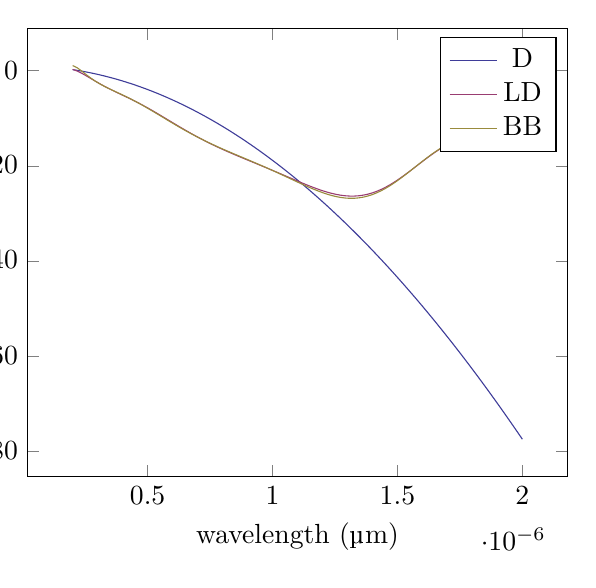
\begin{tikzpicture}[baseline,trim axis left]
\begin{axis}[xlabel=wavelength (\si{\micro\meter}),ylabel=$\epsilon'$]
\addplot[color=colora] coordinates {
(2e-07, 0.20322356523)
(2.18181818182e-07, 0.0518002041146)
(2.36363636364e-07, -0.11277953485)
(2.54545454545e-07, -0.29051293524)
(2.72727272727e-07, -0.481397063843)
(2.90909090909e-07, -0.685428770778)
(3.09090909091e-07, -0.902604689628)
(3.27272727273e-07, -1.13292123757)
(3.45454545455e-07, -1.37637461555)
(3.63636363636e-07, -1.63296080838)
(3.81818181818e-07, -1.90267558498)
(4e-07, -2.18551449849)
(4.18181818182e-07, -2.4814728865)
(4.36363636364e-07, -2.7905458712)
(4.54545454545e-07, -3.11272835961)
(4.72727272727e-07, -3.44801504378)
(4.90909090909e-07, -3.796400401)
(5.09090909091e-07, -4.15787869405)
(5.27272727273e-07, -4.5324439714)
(5.45454545455e-07, -4.92009006751)
(5.63636363636e-07, -5.32081060302)
(5.81818181818e-07, -5.73459898504)
(6e-07, -6.16144840746)
(6.18181818182e-07, -6.60135185113)
(6.36363636364e-07, -7.05430208428)
(6.54545454545e-07, -7.52029166268)
(6.72727272727e-07, -7.99931293006)
(6.90909090909e-07, -8.49135801835)
(7.09090909091e-07, -8.99641884805)
(7.27272727273e-07, -9.5144871285)
(7.45454545455e-07, -10.0455543583)
(7.63636363636e-07, -10.5896118256)
(7.81818181818e-07, -11.1466506084)
(8e-07, -11.7166615751)
(8.18181818182e-07, -12.2996353848)
(8.36363636364e-07, -12.8955624874)
(8.54545454545e-07, -13.5044331245)
(8.72727272727e-07, -14.1262373294)
(8.90909090909e-07, -14.7609649276)
(9.09090909091e-07, -15.4086055373)
(9.27272727273e-07, -16.0691485697)
(9.45454545455e-07, -16.7425832297)
(9.63636363636e-07, -17.428898516)
(9.81818181818e-07, -18.1280832216)
(1e-06, -18.8401259345)
(1.01818181818e-06, -19.5650150379)
(1.03636363636e-06, -20.3027387109)
(1.05454545455e-06, -21.0532849287)
(1.07272727273e-06, -21.8166414635)
(1.09090909091e-06, -22.5927958843)
(1.10909090909e-06, -23.3817355584)
(1.12727272727e-06, -24.1834476508)
(1.14545454545e-06, -24.9979191257)
(1.16363636364e-06, -25.8251367464)
(1.18181818182e-06, -26.665087076)
(1.2e-06, -27.5177564781)
(1.21818181818e-06, -28.3831311171)
(1.23636363636e-06, -29.261196959)
(1.25454545455e-06, -30.1519397717)
(1.27272727273e-06, -31.0553451259)
(1.29090909091e-06, -31.9713983953)
(1.30909090909e-06, -32.9000847575)
(1.32727272727e-06, -33.8413891944)
(1.34545454545e-06, -34.795296493)
(1.36363636364e-06, -35.7617912458)
(1.38181818182e-06, -36.7408578514)
(1.4e-06, -37.7324805155)
(1.41818181818e-06, -38.7366432509)
(1.43636363636e-06, -39.7533298788)
(1.45454545455e-06, -40.7825240289)
(1.47272727273e-06, -41.8242091405)
(1.49090909091e-06, -42.8783684629)
(1.50909090909e-06, -43.9449850559)
(1.52727272727e-06, -45.0240417909)
(1.54545454545e-06, -46.1155213513)
(1.56363636364e-06, -47.2194062333)
(1.58181818182e-06, -48.3356787464)
(1.6e-06, -49.4643210144)
(1.61818181818e-06, -50.6053149759)
(1.63636363636e-06, -51.7586423849)
(1.65454545455e-06, -52.9242848118)
(1.67272727273e-06, -54.1022236442)
(1.69090909091e-06, -55.292440087)
(1.70909090909e-06, -56.494915164)
(1.72727272727e-06, -57.7096297179)
(1.74545454545e-06, -58.9365644115)
(1.76363636364e-06, -60.1756997283)
(1.78181818182e-06, -61.4270159734)
(1.8e-06, -62.6904932739)
(1.81818181818e-06, -63.9661115801)
(1.83636363636e-06, -65.2538506662)
(1.85454545455e-06, -66.5536901308)
(1.87272727273e-06, -67.8656093979)
(1.89090909091e-06, -69.1895877178)
(1.90909090909e-06, -70.5256041678)
(1.92727272727e-06, -71.8736376528)
(1.94545454545e-06, -73.2336669066)
(1.96363636364e-06, -74.6056704923)
(1.98181818182e-06, -75.9896268032)
(2e-06, -77.3855140637)
};
\addlegendentry{D}
\addplot[color=colorb] coordinates {
(2e-07, 0.252315423849)
(2.18181818182e-07, -0.0948185408319)
(2.36363636364e-07, -0.565123571118)
(2.54545454545e-07, -1.10063671894)
(2.72727272727e-07, -1.66253732055)
(2.90909090909e-07, -2.22482729175)
(3.09090909091e-07, -2.77101170623)
(3.27272727273e-07, -3.29246979843)
(3.45454545455e-07, -3.78731567677)
(3.63636363636e-07, -4.25906485906)
(3.81818181818e-07, -4.71492551498)
(4e-07, -5.16389377949)
(4.18181818182e-07, -5.61498414703)
(4.36363636364e-07, -6.07588144042)
(4.54545454545e-07, -6.55214665007)
(4.72727272727e-07, -7.04694848539)
(4.90909090909e-07, -7.56119117679)
(5.09090909091e-07, -8.09387952556)
(5.27272727273e-07, -8.64258310825)
(5.45454545455e-07, -9.20390367814)
(5.63636363636e-07, -9.77389175511)
(5.81818181818e-07, -10.3483900838)
(6e-07, -10.9233013172)
(6.18181818182e-07, -11.4947872486)
(6.36363636364e-07, -12.0594104954)
(6.54545454545e-07, -12.6142295849)
(6.72727272727e-07, -13.156856875)
(6.90909090909e-07, -13.685486818)
(7.09090909091e-07, -14.1989003147)
(7.27272727273e-07, -14.6964495329)
(7.45454545455e-07, -15.1780265991)
(7.63636363636e-07, -15.6440189589)
(7.81818181818e-07, -16.0952538368)
(8e-07, -16.5329340287)
(8.18181818182e-07, -16.9585671401)
(8.36363636364e-07, -17.3738902932)
(8.54545454545e-07, -17.780792221)
(8.72727272727e-07, -18.1812345315)
(8.90909090909e-07, -18.5771737532)
(9.09090909091e-07, -18.9704855675)
(9.27272727273e-07, -19.3628924139)
(9.45454545455e-07, -19.7558954269)
(9.63636363636e-07, -20.150711456)
(9.81818181818e-07, -20.5482157419)
(1e-06, -20.9488906909)
(1.01818181818e-06, -21.3527811092)
(1.03636363636e-06, -21.7594562484)
(1.05454545455e-06, -22.1679790528)
(1.07272727273e-06, -22.5768831107)
(1.09090909091e-06, -22.9841579631)
(1.10909090909e-06, -23.3872436195)
(1.12727272727e-06, -23.7830353437)
(1.14545454545e-06, -24.1678999802)
(1.16363636364e-06, -24.5377052718)
(1.18181818182e-06, -24.8878637218)
(1.2e-06, -25.2133925621)
(1.21818181818e-06, -25.5089912346)
(1.23636363636e-06, -25.7691374586)
(1.25454545455e-06, -25.9882023917)
(1.27272727273e-06, -26.1605845748)
(1.29090909091e-06, -26.2808612855)
(1.30909090909e-06, -26.3439546195)
(1.32727272727e-06, -26.3453081511)
(1.34545454545e-06, -26.2810684787)
(1.36363636364e-06, -26.1482644867)
(1.38181818182e-06, -25.9449759233)
(1.4e-06, -25.6704820895)
(1.41818181818e-06, -25.3253812476)
(1.43636363636e-06, -24.9116719255)
(1.45454545455e-06, -24.4327886955)
(1.47272727273e-06, -23.8935872257)
(1.49090909091e-06, -23.3002762983)
(1.50909090909e-06, -22.6602978391)
(1.52727272727e-06, -21.9821594752)
(1.54545454545e-06, -21.2752273753)
(1.56363636364e-06, -20.5494897806)
(1.58181818182e-06, -19.8153034161)
(1.6e-06, -19.083135712)
(1.61818181818e-06, -18.3633154199)
(1.63636363636e-06, -17.6658028767)
(1.65454545455e-06, -16.999989055)
(1.67272727273e-06, -16.3745299263)
(1.69090909091e-06, -15.7972198529)
(1.70909090909e-06, -15.2749050095)
(1.72727272727e-06, -14.8134354381)
(1.74545454545e-06, -14.4176524264)
(1.76363636364e-06, -14.0914065407)
(1.78181818182e-06, -13.8376008474)
(1.8e-06, -13.658253569)
(1.81818181818e-06, -13.5545745555)
(1.83636363636e-06, -13.5270503977)
(1.85454545455e-06, -13.5755336635)
(1.87272727273e-06, -13.6993325024)
(1.89090909091e-06, -13.8972976524)
(1.90909090909e-06, -14.1679046457)
(1.92727272727e-06, -14.5093296945)
(1.94545454545e-06, -14.9195183307)
(1.96363636364e-06, -15.3962463582)
(1.98181818182e-06, -15.9371730605)
(2e-06, -16.5398868881)
};
\addlegendentry{LD}
\addplot[color=colorc] coordinates {
(2e-07, 1.05046378396)
(2.18181818182e-07, 0.594482942693)
(2.36363636364e-07, -0.100504672608)
(2.54545454545e-07, -0.85395781284)
(2.72727272727e-07, -1.5746320394)
(2.90909090909e-07, -2.22561431927)
(3.09090909091e-07, -2.80192575417)
(3.27272727273e-07, -3.31566310266)
(3.45454545455e-07, -3.78591981878)
(3.63636363636e-07, -4.23244246209)
(3.81818181818e-07, -4.6722081106)
(4e-07, -5.11804871249)
(4.18181818182e-07, -5.57851491631)
(4.36363636364e-07, -6.05837093924)
(4.54545454545e-07, -6.55932857645)
(4.72727272727e-07, -7.08080226317)
(4.90909090909e-07, -7.62058325486)
(5.09090909091e-07, -8.17539869492)
(5.27272727273e-07, -8.74135581895)
(5.45454545455e-07, -9.31428603972)
(5.63636363636e-07, -9.89000740561)
(5.81818181818e-07, -10.4645226077)
(6e-07, -11.0341665086)
(6.18181818182e-07, -11.5957136992)
(6.36363636364e-07, -12.146453591)
(6.54545454545e-07, -12.6842382678)
(6.72727272727e-07, -13.207506763)
(6.90909090909e-07, -13.7152884949)
(7.09090909091e-07, -14.2071881344)
(7.27272727273e-07, -14.6833540522)
(7.45454545455e-07, -15.1444325511)
(7.63636363636e-07, -15.5915102219)
(7.81818181818e-07, -16.0260470783)
(8e-07, -16.4498018035)
(8.18181818182e-07, -16.8647544581)
(8.36363636364e-07, -17.2730251427)
(8.54545454545e-07, -17.6767934796)
(8.72727272727e-07, -18.0782195419)
(8.90909090909e-07, -18.4793677967)
(9.09090909091e-07, -18.882135093)
(9.27272727273e-07, -19.2881833956)
(9.45454545455e-07, -19.6988776844)
(9.63636363636e-07, -20.1152292266)
(9.81818181818e-07, -20.5378442974)
(1e-06, -20.9668783781)
(1.01818181818e-06, -21.4019959055)
(1.03636363636e-06, -21.8423357754)
(1.05454545455e-06, -22.2864830143)
(1.07272727273e-06, -22.7324473137)
(1.09090909091e-06, -23.1776494566)
(1.10909090909e-06, -23.6189170311)
(1.12727272727e-06, -24.0524911986)
(1.14545454545e-06, -24.4740466146)
(1.16363636364e-06, -24.8787268525)
(1.18181818182e-06, -25.2611977824)
(1.2e-06, -25.6157212575)
(1.21818181818e-06, -25.93625108)
(1.23636363636e-06, -26.2165525085)
(1.25454545455e-06, -26.4503454875)
(1.27272727273e-06, -26.6314703246)
(1.29090909091e-06, -26.7540727598)
(1.30909090909e-06, -26.8128033728)
(1.32727272727e-06, -26.8030242258)
(1.34545454545e-06, -26.7210137678)
(1.36363636364e-06, -26.5641595914)
(1.38181818182e-06, -26.331127875)
(1.4e-06, -26.0219984863)
(1.41818181818e-06, -25.6383558652)
(1.43636363636e-06, -25.1833279513)
(1.45454545455e-06, -24.6615684249)
(1.47272727273e-06, -24.0791811234)
(1.49090909091e-06, -23.4435893199)
(1.50909090909e-06, -22.7633562036)
(1.52727272727e-06, -22.0479660082)
(1.54545454545e-06, -21.3075774968)
(1.56363636364e-06, -20.5527627291)
(1.58181818182e-06, -19.7942441787)
(1.6e-06, -19.0426423935)
(1.61818181818e-06, -18.308244693)
(1.63636363636e-06, -17.6008031204)
(1.65454545455e-06, -16.9293672891)
(1.67272727273e-06, -16.3021551451)
(1.69090909091e-06, -15.7264622406)
(1.70909090909e-06, -15.2086080281)
(1.72727272727e-06, -14.7539160553)
(1.74545454545e-06, -14.366723792)
(1.76363636364e-06, -14.0504171494)
(1.78181818182e-06, -13.8074844927)
(1.8e-06, -13.6395850475)
(1.81818181818e-06, -13.5476269462)
(1.83636363636e-06, -13.5318506974)
(1.85454545455e-06, -13.5919144882)
(1.87272727273e-06, -13.726978399)
(1.89090909091e-06, -13.9357852679)
(1.90909090909e-06, -14.2167365499)
(1.92727272727e-06, -14.5679620548)
(1.94545454545e-06, -14.9873829104)
(1.96363636364e-06, -15.4727674692)
(1.98181818182e-06, -16.0217801748)
(2e-06, -16.632023624)
};
\addlegendentry{BB}
\end{axis}
\end{tikzpicture}%
\\
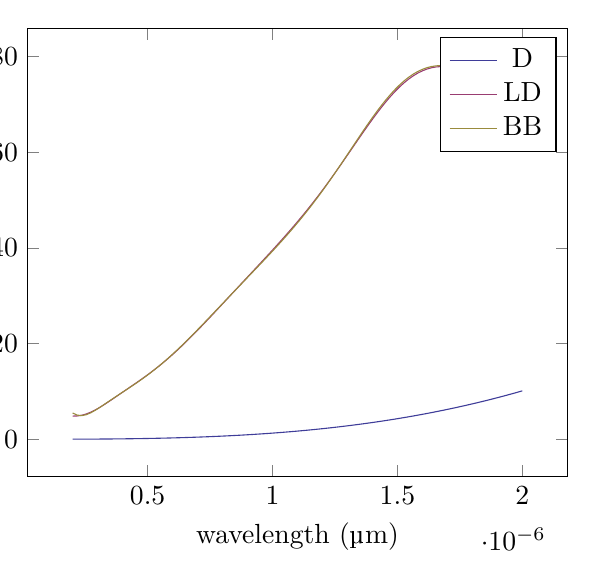
\begin{tikzpicture}[baseline,trim axis left]
\begin{axis}[xlabel=wavelength (\si{\micro\meter}),ylabel=$\epsilon''$]
\addplot[color=colora] coordinates {
(2e-07, 0.0102822970058)
(2.18181818182e-07, 0.0133487955581)
(2.36363636364e-07, 0.0169712355186)
(2.54545454545e-07, 0.0211958762781)
(2.72727272727e-07, 0.0260689606656)
(2.90909090909e-07, 0.0316367136779)
(3.09090909091e-07, 0.0379453412121)
(3.27272727273e-07, 0.0450410287982)
(3.45454545455e-07, 0.0529699403325)
(3.63636363636e-07, 0.0617782168134)
(3.81818181818e-07, 0.0715119750776)
(4e-07, 0.082217306538)
(4.18181818182e-07, 0.0939402759232)
(4.36363636364e-07, 0.106726920018)
(4.54545454545e-07, 0.120623246407)
(4.72727272727e-07, 0.135675232216)
(4.90909090909e-07, 0.151928822863)
(5.09090909091e-07, 0.169429930799)
(5.27272727273e-07, 0.188224434266)
(5.45454545455e-07, 0.20835817604)
(5.63636363636e-07, 0.229876962191)
(5.81818181818e-07, 0.252826560836)
(6e-07, 0.277252700898)
(6.18181818182e-07, 0.303201070866)
(6.36363636364e-07, 0.330717317555)
(6.54545454545e-07, 0.359847044876)
(6.72727272727e-07, 0.3906358126)
(6.90909090909e-07, 0.423129135127)
(7.09090909091e-07, 0.45737248026)
(7.27272727273e-07, 0.493411267983)
(7.45454545455e-07, 0.531290869233)
(7.63636363636e-07, 0.571056604685)
(7.81818181818e-07, 0.612753743534)
(8e-07, 0.656427502282)
(8.18181818182e-07, 0.702123043528)
(8.36363636364e-07, 0.74988547476)
(8.54545454545e-07, 0.799759847149)
(8.72727272727e-07, 0.851791154353)
(8.90909090909e-07, 0.906024331313)
(9.09090909091e-07, 0.962504253064)
(9.27272727273e-07, 1.02127573354)
(9.45454545455e-07, 1.08238352439)
(9.63636363636e-07, 1.14587231378)
(9.81818181818e-07, 1.21178672526)
(1e-06, 1.2801713165)
(1.01818181818e-06, 1.35107057821)
(1.03636363636e-06, 1.42452893292)
(1.05454545455e-06, 1.50059073381)
(1.07272727273e-06, 1.57930026359)
(1.09090909091e-06, 1.66070173328)
(1.10909090909e-06, 1.74483928112)
(1.12727272727e-06, 1.83175697139)
(1.14545454545e-06, 1.92149879326)
(1.16363636364e-06, 2.01410865966)
(1.18181818182e-06, 2.10963040613)
(1.2e-06, 2.20810778972)
(1.21818181818e-06, 2.30958448783)
(1.23636363636e-06, 2.41410409709)
(1.25454545455e-06, 2.52171013226)
(1.27272727273e-06, 2.6324460251)
(1.29090909091e-06, 2.74635512325)
(1.30909090909e-06, 2.86348068916)
(1.32727272727e-06, 2.98386589896)
(1.34545454545e-06, 3.10755384138)
(1.36363636364e-06, 3.23458751665)
(1.38181818182e-06, 3.36500983542)
(1.4e-06, 3.49886361766)
(1.41818181818e-06, 3.63619159164)
(1.43636363636e-06, 3.77703639278)
(1.45454545455e-06, 3.92144056266)
(1.47272727273e-06, 4.06944654791)
(1.49090909091e-06, 4.22109669917)
(1.50909090909e-06, 4.37643327006)
(1.52727272727e-06, 4.53549841609)
(1.54545454545e-06, 4.69833419367)
(1.56363636364e-06, 4.86498255906)
(1.58181818182e-06, 5.03548536732)
(1.6e-06, 5.20988437132)
(1.61818181818e-06, 5.38822122071)
(1.63636363636e-06, 5.5705374609)
(1.65454545455e-06, 5.75687453207)
(1.67272727273e-06, 5.94727376816)
(1.69090909091e-06, 6.1417763959)
(1.70909090909e-06, 6.34042353377)
(1.72727272727e-06, 6.54325619108)
(1.74545454545e-06, 6.75031526694)
(1.76363636364e-06, 6.96164154934)
(1.78181818182e-06, 7.17727571415)
(1.8e-06, 7.39725832418)
(1.81818181818e-06, 7.62162982819)
(1.83636363636e-06, 7.85043056003)
(1.85454545455e-06, 8.0837007376)
(1.87272727273e-06, 8.32148046198)
(1.89090909091e-06, 8.56380971651)
(1.90909090909e-06, 8.8107283658)
(1.92727272727e-06, 9.0622761549)
(1.94545454545e-06, 9.31849270834)
(1.96363636364e-06, 9.57941752924)
(1.98181818182e-06, 9.84508999842)
(2e-06, 10.1155493735)
};
\addlegendentry{D}
\addplot[color=colorb] coordinates {
(2e-07, 4.84279765753)
(2.18181818182e-07, 4.86354834929)
(2.36363636364e-07, 5.01240232436)
(2.54545454545e-07, 5.28442745416)
(2.72727272727e-07, 5.66498812065)
(2.90909090909e-07, 6.13575893618)
(3.09090909091e-07, 6.676998052)
(3.27272727273e-07, 7.26904235788)
(3.45454545455e-07, 7.89383137937)
(3.63636363636e-07, 8.53638493596)
(3.81818181818e-07, 9.18589059095)
(4e-07, 9.83612658053)
(4.18181818182e-07, 10.4851698089)
(4.36363636364e-07, 11.1345554675)
(4.54545454545e-07, 11.7881649294)
(4.72727272727e-07, 12.4511078178)
(4.90909090909e-07, 13.1287788628)
(5.09090909091e-07, 13.8261691241)
(5.27272727273e-07, 14.5474329075)
(5.45454545455e-07, 15.2956681516)
(5.63636363636e-07, 16.0728536964)
(5.81818181818e-07, 16.879890303)
(6e-07, 17.7167034386)
(6.18181818182e-07, 18.5823782077)
(6.36363636364e-07, 19.4753072801)
(6.54545454545e-07, 20.3933403273)
(6.72727272727e-07, 21.3339285191)
(6.90909090909e-07, 22.294260656)
(7.09090909091e-07, 23.2713891674)
(7.27272727273e-07, 24.2623450096)
(7.45454545455e-07, 25.264240847)
(7.63636363636e-07, 26.2743620332)
(7.81818181818e-07, 27.2902449863)
(8e-07, 28.3097426392)
(8.18181818182e-07, 29.3310767832)
(8.36363636364e-07, 30.3528772969)
(8.54545454545e-07, 31.3742084617)
(8.72727272727e-07, 32.3945827707)
(8.90909090909e-07, 33.4139628331)
(9.09090909091e-07, 34.4327521294)
(9.27272727273e-07, 35.4517754765)
(9.45454545455e-07, 36.4722501123)
(9.63636363636e-07, 37.4957482988)
(9.81818181818e-07, 38.5241522878)
(1e-06, 39.5596023956)
(1.01818181818e-06, 40.6044388153)
(1.03636363636e-06, 41.6611376687)
(1.05454545455e-06, 42.7322416876)
(1.07272727273e-06, 43.8202858326)
(1.09090909091e-06, 44.9277181264)
(1.10909090909e-06, 46.0568160187)
(1.12727272727e-06, 47.2095987181)
(1.14545454545e-06, 48.3877361521)
(1.16363636364e-06, 49.592455539)
(1.18181818182e-06, 50.8244469896)
(1.2e-06, 52.0837700911)
(1.21818181818e-06, 53.3697640386)
(1.23636363636e-06, 54.6809645369)
(1.25454545455e-06, 56.0150313475)
(1.27272727273e-06, 57.3686909318)
(1.29090909091e-06, 58.7376990536)
(1.30909090909e-06, 60.1168283579)
(1.32727272727e-06, 61.4998857433)
(1.34545454545e-06, 62.8797636911)
(1.36363636364e-06, 64.2485285641)
(1.38181818182e-06, 65.5975472123)
(1.4e-06, 66.9176510758)
(1.41818181818e-06, 68.1993344817)
(1.43636363636e-06, 69.4329811819)
(1.45454545455e-06, 70.6091106272)
(1.47272727273e-06, 71.718633318)
(1.49090909091e-06, 72.7531030881)
(1.50909090909e-06, 73.7049535997)
(1.52727272727e-06, 74.5677067987)
(1.54545454545e-06, 75.3361426021)
(1.56363636364e-06, 76.0064215519)
(1.58181818182e-06, 76.5761553152)
(1.6e-06, 77.0444234133)
(1.61818181818e-06, 77.4117380509)
(1.63636363636e-06, 77.6799620412)
(1.65454545455e-06, 77.8521873044)
(1.67272727273e-06, 77.9325830766)
(1.69090909091e-06, 77.9262237478)
(1.70909090909e-06, 77.8389061855)
(1.72727272727e-06, 77.6769656441)
(1.74545454545e-06, 77.4470980726)
(1.76363636364e-06, 77.1561950406)
(1.78181818182e-06, 76.8111957798)
(1.8e-06, 76.4189591666)
(1.81818181818e-06, 75.9861569571)
(1.83636363636e-06, 75.5191883217)
(1.85454545455e-06, 75.0241147338)
(1.87272727273e-06, 74.5066135606)
(1.89090909091e-06, 73.9719482528)
(1.90909090909e-06, 73.4249527977)
(1.92727272727e-06, 72.8700280529)
(1.94545454545e-06, 72.3111476532)
(1.96363636364e-06, 71.7518713579)
(1.98181818182e-06, 71.1953639311)
(2e-06, 70.6444179018)
};
\addlegendentry{LD}
\addplot[color=colorc] coordinates {
(2e-07, 5.4875856574)
(2.18181818182e-07, 5.04046509054)
(2.36363636364e-07, 4.94200743216)
(2.54545454545e-07, 5.13364971578)
(2.72727272727e-07, 5.53329001958)
(2.90909090909e-07, 6.06548654664)
(3.09090909091e-07, 6.67085949615)
(3.27272727273e-07, 7.30804209878)
(3.45454545455e-07, 7.95198650953)
(3.63636363636e-07, 8.59050896282)
(3.81818181818e-07, 9.22044122321)
(4e-07, 9.84421988054)
(4.18181818182e-07, 10.4672560955)
(4.36363636364e-07, 11.0961038143)
(4.54545454545e-07, 11.7372919634)
(4.72727272727e-07, 12.3966468578)
(4.90909090909e-07, 13.0789479816)
(5.09090909091e-07, 13.7877962888)
(5.27272727273e-07, 14.5256104215)
(5.45454545455e-07, 15.2936956113)
(5.63636363636e-07, 16.0923512217)
(5.81818181818e-07, 16.9209970264)
(6e-07, 17.7783071395)
(6.18181818182e-07, 18.6623456498)
(6.36363636364e-07, 19.5707007409)
(6.54545454545e-07, 20.5006153469)
(6.72727272727e-07, 21.4491128356)
(6.90909090909e-07, 22.4131162659)
(7.09090909091e-07, 23.3895596931)
(7.27272727273e-07, 24.3754899642)
(7.45454545455e-07, 25.368157521)
(7.63636363636e-07, 26.3650949399)
(7.81818181818e-07, 27.3641825863)
(8e-07, 28.3636988822)
(8.18181818182e-07, 29.3623599823)
(8.36363636364e-07, 30.3593425892)
(8.54545454545e-07, 31.3542955082)
(8.72727272727e-07, 32.3473388837)
(8.90909090909e-07, 33.3390525508)
(9.09090909091e-07, 34.3304546727)
(9.27272727273e-07, 35.3229718052)
(9.45454545455e-07, 36.3184014247)
(9.63636363636e-07, 37.3188677816)
(9.81818181818e-07, 38.3267717279)
(1e-06, 39.3447349391)
(1.01818181818e-06, 40.37553872)
(1.03636363636e-06, 41.4220573909)
(1.05454545455e-06, 42.487186099)
(1.07272727273e-06, 43.573762829)
(1.09090909091e-06, 44.6844844093)
(1.10909090909e-06, 45.8218164525)
(1.12727272727e-06, 46.9878974496)
(1.14545454545e-06, 48.1844376717)
(1.16363636364e-06, 49.4126141333)
(1.18181818182e-06, 50.6729636213)
(1.2e-06, 51.9652766809)
(1.21818181818e-06, 53.2884964181)
(1.23636363636e-06, 54.6406269462)
(1.25454545455e-06, 56.0186571715)
(1.27272727273e-06, 57.4185062379)
(1.29090909091e-06, 58.8349971876)
(1.30909090909e-06, 60.2618650969)
(1.32727272727e-06, 61.6918050049)
(1.34545454545e-06, 63.1165633081)
(1.36363636364e-06, 64.5270739763)
(1.38181818182e-06, 65.9136380931)
(1.4e-06, 67.2661420575)
(1.41818181818e-06, 68.5743066281)
(1.43636363636e-06, 69.8279561915)
(1.45454545455e-06, 71.0172955451)
(1.47272727273e-06, 72.1331803703)
(1.49090909091e-06, 73.1673676099)
(1.50909090909e-06, 74.1127331579)
(1.52727272727e-06, 74.9634465111)
(1.54545454545e-06, 75.7150950543)
(1.56363636364e-06, 76.364754126)
(1.58181818182e-06, 76.9110025718)
(1.6e-06, 77.3538867935)
(1.61818181818e-06, 77.6948390649)
(1.63636363636e-06, 77.9365579255)
(1.65454545455e-06, 78.0828596956)
(1.67272727273e-06, 78.1385105968)
(1.69090909091e-06, 78.1090486975)
(1.70909090909e-06, 78.0006040789)
(1.72727272727e-06, 77.8197243961)
(1.74545454545e-06, 77.5732115666)
(1.76363636364e-06, 77.2679738021)
(1.78181818182e-06, 76.9108957314)
(1.8e-06, 76.5087280446)
(1.81818181818e-06, 76.0679969603)
(1.83636363636e-06, 75.5949329236)
(1.85454545455e-06, 75.0954172761)
(1.87272727273e-06, 74.5749451819)
(1.89090909091e-06, 74.038602833)
(1.90909090909e-06, 73.4910568456)
(1.92727272727e-06, 72.9365537693)
(1.94545454545e-06, 72.3789277377)
(1.96363636364e-06, 71.8216144433)
(1.98181818182e-06, 71.2676698242)
(2e-06, 70.7197920583)
};
\addlegendentry{BB}
\end{axis}
\end{tikzpicture}%
\\
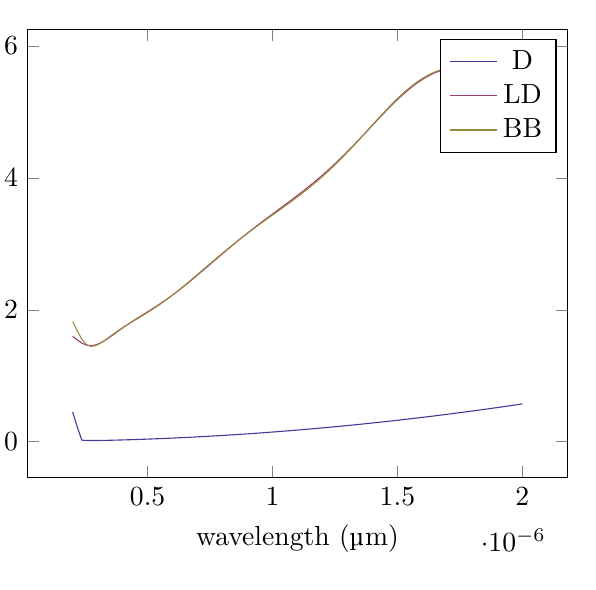
\begin{tikzpicture}[baseline,trim axis left]
\begin{axis}[xlabel=wavelength (\si{\micro\meter}),ylabel=$n'$]
\addplot[color=colora] coordinates {
(2e-07, 0.450947383673)
(2.18181818182e-07, 0.229447968912)
(2.36363636364e-07, 0.0251970279077)
(2.54545454545e-07, 0.0196494427858)
(2.72727272727e-07, 0.0187794548242)
(2.90909090909e-07, 0.0191013755765)
(3.09090909091e-07, 0.0199656656425)
(3.27272727273e-07, 0.0211540094074)
(3.45454545455e-07, 0.0225710000167)
(3.63636363636e-07, 0.024167951184)
(3.81818181818e-07, 0.025917300132)
(4e-07, 0.0278022290692)
(4.18181818182e-07, 0.0298118763024)
(4.36363636364e-07, 0.0319389057993)
(4.54545454545e-07, 0.0341781797787)
(4.72727272727e-07, 0.0365259900867)
(4.90909090909e-07, 0.0389795913648)
(5.09090909091e-07, 0.0415369060074)
(5.27272727273e-07, 0.0441963313025)
(5.45454545455e-07, 0.0469566096684)
(5.63636363636e-07, 0.049816739126)
(5.81818181818e-07, 0.0527759101574)
(6e-07, 0.0558334602998)
(6.18181818182e-07, 0.0589888409239)
(6.36363636364e-07, 0.0622415925467)
(6.54545454545e-07, 0.065591326228)
(6.72727272727e-07, 0.0690377093738)
(6.90909090909e-07, 0.0725804547751)
(7.09090909091e-07, 0.0762193120563)
(7.27272727273e-07, 0.0799540609392)
(7.45454545455e-07, 0.0837845058875)
(7.63636363636e-07, 0.0877104718159)
(7.81818181818e-07, 0.0917318006239)
(8e-07, 0.095848348378)
(8.18181818182e-07, 0.100059983003)
(8.36363636364e-07, 0.104366582382)
(8.54545454545e-07, 0.10876803278)
(8.72727272727e-07, 0.113264227533)
(8.90909090909e-07, 0.117855065946)
(9.09090909091e-07, 0.122540452375)
(9.27272727273e-07, 0.127320295437)
(9.45454545455e-07, 0.132194507354)
(9.63636363636e-07, 0.137163003384)
(9.81818181818e-07, 0.142225701339)
(1e-06, 0.147382521168)
(1.01818181818e-06, 0.152633384602)
(1.03636363636e-06, 0.157978214841)
(1.05454545455e-06, 0.163416936292)
(1.07272727273e-06, 0.168949474331)
(1.09090909091e-06, 0.174575755099)
(1.10909090909e-06, 0.18029570533)
(1.12727272727e-06, 0.18610925219)
(1.14545454545e-06, 0.192016323143)
(1.16363636364e-06, 0.198016845829)
(1.18181818182e-06, 0.204110747961)
(1.2e-06, 0.210297957227)
(1.21818181818e-06, 0.216578401209)
(1.23636363636e-06, 0.222952007309)
(1.25454545455e-06, 0.229418702684)
(1.27272727273e-06, 0.235978414187)
(1.29090909091e-06, 0.242631068316)
(1.30909090909e-06, 0.249376591166)
(1.32727272727e-06, 0.256214908389)
(1.34545454545e-06, 0.263145945154)
(1.36363636364e-06, 0.270169626122)
(1.38181818182e-06, 0.277285875404)
(1.4e-06, 0.284494616545)
(1.41818181818e-06, 0.291795772496)
(1.43636363636e-06, 0.299189265591)
(1.45454545455e-06, 0.30667501753)
(1.47272727273e-06, 0.314252949363)
(1.49090909091e-06, 0.32192298147)
(1.50909090909e-06, 0.329685033552)
(1.52727272727e-06, 0.337539024615)
(1.54545454545e-06, 0.345484872963)
(1.56363636364e-06, 0.353522496181)
(1.58181818182e-06, 0.361651811134)
(1.6e-06, 0.369872733955)
(1.61818181818e-06, 0.378185180038)
(1.63636363636e-06, 0.386589064033)
(1.65454545455e-06, 0.395084299837)
(1.67272727273e-06, 0.403670800596)
(1.69090909091e-06, 0.412348478694)
(1.70909090909e-06, 0.421117245753)
(1.72727272727e-06, 0.429977012627)
(1.74545454545e-06, 0.438927689405)
(1.76363636364e-06, 0.4479691854)
(1.78181818182e-06, 0.457101409155)
(1.8e-06, 0.466324268437)
(1.81818181818e-06, 0.475637670237)
(1.83636363636e-06, 0.485041520771)
(1.85454545455e-06, 0.494535725476)
(1.87272727273e-06, 0.50412018901)
(1.89090909091e-06, 0.513794815257)
(1.90909090909e-06, 0.523559507319)
(1.92727272727e-06, 0.533414167523)
(1.94545454545e-06, 0.543358697419)
(1.96363636364e-06, 0.553392997782)
(1.98181818182e-06, 0.563516968608)
(2e-06, 0.573730509123)
};
\addlegendentry{D}
\addplot[color=colorb] coordinates {
(2e-07, 1.59713518388)
(2.18181818182e-07, 1.54428850933)
(2.36363636364e-07, 1.4965018538)
(2.54545454545e-07, 1.46580930487)
(2.72727272727e-07, 1.45625717573)
(2.90909090909e-07, 1.46660162162)
(3.09090909091e-07, 1.49300905342)
(3.27272727273e-07, 1.53092511578)
(3.45454545455e-07, 1.57607814169)
(3.63636363636e-07, 1.62493463605)
(3.81818181818e-07, 1.67486417798)
(4e-07, 1.72414398277)
(4.18181818182e-07, 1.77186327169)
(4.36363636364e-07, 1.81776572643)
(4.54545454545e-07, 1.8620643764)
(4.72727272727e-07, 1.90525952886)
(4.90909090909e-07, 1.94798217328)
(5.09090909091e-07, 1.99087469302)
(5.27272727273e-07, 2.03451102931)
(5.45454545455e-07, 2.07935174965)
(5.63636363636e-07, 2.12572618367)
(5.81818181818e-07, 2.17383321308)
(6e-07, 2.22375336848)
(6.18181818182e-07, 2.27546663533)
(6.36363636364e-07, 2.32887215603)
(6.54545454545e-07, 2.38380750545)
(6.72727272727e-07, 2.44006630755)
(6.90909090909e-07, 2.49741367976)
(7.09090909091e-07, 2.55559941814)
(7.27272727273e-07, 2.61436905836)
(7.45454545455e-07, 2.67347304047)
(7.63636363636e-07, 2.73267422358)
(7.81818181818e-07, 2.79175397757)
(8e-07, 2.85051704514)
(8.18181818182e-07, 2.90879533139)
(8.36363636364e-07, 2.96645074604)
(8.54545454545e-07, 3.02337719728)
(8.72727272727e-07, 3.07950181672)
(8.90909090909e-07, 3.13478548039)
(9.09090909091e-07, 3.18922268047)
(9.27272727273e-07, 3.2428407955)
(9.45454545455e-07, 3.29569880106)
(9.63636363636e-07, 3.34788545916)
(9.81818181818e-07, 3.39951702126)
(1e-06, 3.45073447713)
(1.01818181818e-06, 3.50170037972)
(1.03636363636e-06, 3.55259527473)
(1.05454545455e-06, 3.60361376327)
(1.07272727273e-06, 3.654960226)
(1.09090909091e-06, 3.70684423976)
(1.10909090909e-06, 3.7594757204)
(1.12727272727e-06, 3.81305983168)
(1.14545454545e-06, 3.86779170703)
(1.16363636364e-06, 3.92385104141)
(1.18181818182e-06, 3.98139662244)
(1.2e-06, 4.04056088532)
(1.21818181818e-06, 4.10144459277)
(1.23636363636e-06, 4.16411175987)
(1.25454545455e-06, 4.22858496304)
(1.27272727273e-06, 4.29484119015)
(1.29090909091e-06, 4.36280840405)
(1.30909090909e-06, 4.43236300079)
(1.32727272727e-06, 4.50332834475)
(1.34545454545e-06, 4.57547455235)
(1.36363636364e-06, 4.64851967135)
(1.38181818182e-06, 4.72213236297)
(1.4e-06, 4.79593613843)
(1.41818181818e-06, 4.86951513194)
(1.43636363636e-06, 4.94242131187)
(1.45454545455e-06, 5.01418294731)
(1.47272727273e-06, 5.08431406491)
(1.49090909091e-06, 5.1523245591)
(1.50909090909e-06, 5.21773056637)
(1.52727272727e-06, 5.28006468598)
(1.54545454545e-06, 5.33888563156)
(1.56363636364e-06, 5.39378692917)
(1.58181818182e-06, 5.44440433731)
(1.6e-06, 5.49042174495)
(1.61818181818e-06, 5.53157539893)
(1.63636363636e-06, 5.56765641151)
(1.65454545455e-06, 5.59851159375)
(1.67272727273e-06, 5.62404274334)
(1.69090909091e-06, 5.64420457992)
(1.70909090909e-06, 5.65900156519)
(1.72727272727e-06, 5.66848386718)
(1.74545454545e-06, 5.67274273084)
(1.76363636364e-06, 5.67190550298)
(1.78181818182e-06, 5.66613053353)
(1.8e-06, 5.65560214045)
(1.81818181818e-06, 5.64052578772)
(1.83636363636e-06, 5.62112358696)
(1.85454545455e-06, 5.59763019685)
(1.87272727273e-06, 5.57028916246)
(1.89090909091e-06, 5.53934970902)
(1.90909090909e-06, 5.50506398331)
(1.92727272727e-06, 5.46768471936)
(1.94545454545e-06, 5.42746329392)
(1.96363636364e-06, 5.3846481301)
(1.98181818182e-06, 5.33948340443)
(2e-06, 5.29220801164)
};
\addlegendentry{LD}
\addplot[color=colorc] coordinates {
(2e-07, 1.82176942122)
(2.18181818182e-07, 1.68372863565)
(2.36363636364e-07, 1.55604058851)
(2.54545454545e-07, 1.47482763877)
(2.72727272727e-07, 1.44539730019)
(2.90909090909e-07, 1.45521572207)
(3.09090909091e-07, 1.48887272839)
(3.27272727273e-07, 1.53449772932)
(3.45454545455e-07, 1.58450448643)
(3.63636363636e-07, 1.63464261284)
(3.81818181818e-07, 1.68291843445)
(4e-07, 1.72874728808)
(4.18181818182e-07, 1.77235483277)
(4.36363636364e-07, 1.81437515249)
(4.54545454545e-07, 1.85559215809)
(4.72727272727e-07, 1.89678192091)
(4.90909090909e-07, 1.93862439208)
(5.09090909091e-07, 1.98166143171)
(5.27272727273e-07, 2.02628446582)
(5.45454545455e-07, 2.07273994704)
(5.63636363636e-07, 2.12114450269)
(5.81818181818e-07, 2.17150444774)
(6e-07, 2.22373637811)
(6.18181818182e-07, 2.27768698044)
(6.36363636364e-07, 2.33315112856)
(6.54545454545e-07, 2.38988791049)
(6.72727272727e-07, 2.44763455166)
(6.90909090909e-07, 2.50611835795)
(7.09090909091e-07, 2.56506686196)
(7.27272727273e-07, 2.62421636304)
(7.45454545455e-07, 2.68331903421)
(7.63636363636e-07, 2.74214874532)
(7.81818181818e-07, 2.80050574471)
(8e-07, 2.85822020892)
(8.18181818182e-07, 2.91515500776)
(8.36363636364e-07, 2.97120743071)
(8.54545454545e-07, 3.02631021534)
(8.72727272727e-07, 3.0804318475)
(8.90909090909e-07, 3.13357622147)
(9.09090909091e-07, 3.18578172368)
(9.27272727273e-07, 3.23711979669)
(9.45454545455e-07, 3.28769303145)
(9.63636363636e-07, 3.33763282722)
(9.81818181818e-07, 3.38709664946)
(1e-06, 3.43626490745)
(1.01818181818e-06, 3.48533746611)
(1.03636363636e-06, 3.53452980038)
(1.05454545455e-06, 3.58406879743)
(1.07272727273e-06, 3.63418821059)
(1.09090909091e-06, 3.68512377203)
(1.10909090909e-06, 3.73710797721)
(1.12727272727e-06, 3.79036456522)
(1.14545454545e-06, 3.8451027351)
(1.16363636364e-06, 3.90151115868)
(1.18181818182e-06, 3.95975187706)
(1.2e-06, 4.01995419782)
(1.21818181818e-06, 4.08220874346)
(1.23636363636e-06, 4.14656183586)
(1.25454545455e-06, 4.21301043267)
(1.27272727273e-06, 4.28149785645)
(1.29090909091e-06, 4.35191057021)
(1.30909090909e-06, 4.42407624991)
(1.32727272727e-06, 4.49776338091)
(1.34545454545e-06, 4.57268255899)
(1.36363636364e-06, 4.64848960799)
(1.38181818182e-06, 4.72479053782)
(1.4e-06, 4.80114826494)
(1.41818181818e-06, 4.87709091156)
(1.43636363636e-06, 4.95212139874)
(1.45454545455e-06, 5.02572796416)
(1.47272727273e-06, 5.09739517521)
(1.49090909091e-06, 5.16661497907)
(1.50909090909e-06, 5.23289733571)
(1.52727272727e-06, 5.29578001684)
(1.54545454545e-06, 5.35483721762)
(1.56363636364e-06, 5.40968671243)
(1.58181818182e-06, 5.4599953817)
(1.6e-06, 5.50548303434)
(1.61818181818e-06, 5.54592454289)
(1.63636363636e-06, 5.58115038782)
(1.65454545455e-06, 5.61104577133)
(1.67272727273e-06, 5.63554850518)
(1.69090909091e-06, 5.65464590351)
(1.70909090909e-06, 5.66837092001)
(1.72727272727e-06, 5.67679776321)
(1.74545454545e-06, 5.68003720619)
(1.76363636364e-06, 5.67823178178)
(1.78181818182e-06, 5.67155102427)
(1.8e-06, 5.6601868865)
(1.81818181818e-06, 5.64434942966)
(1.83636363636e-06, 5.62426285325)
(1.85454545455e-06, 5.60016190639)
(1.87272727273e-06, 5.57228869899)
(1.89090909091e-06, 5.54088991278)
(1.90909090909e-06, 5.50621439788)
(1.92727272727e-06, 5.46851113)
(1.94545454545e-06, 5.42802749623)
(1.96363636364e-06, 5.38500787311)
(1.98181818182e-06, 5.33969245902)
(2e-06, 5.29231632301)
};
\addlegendentry{BB}
\end{axis}
\end{tikzpicture}%
\\
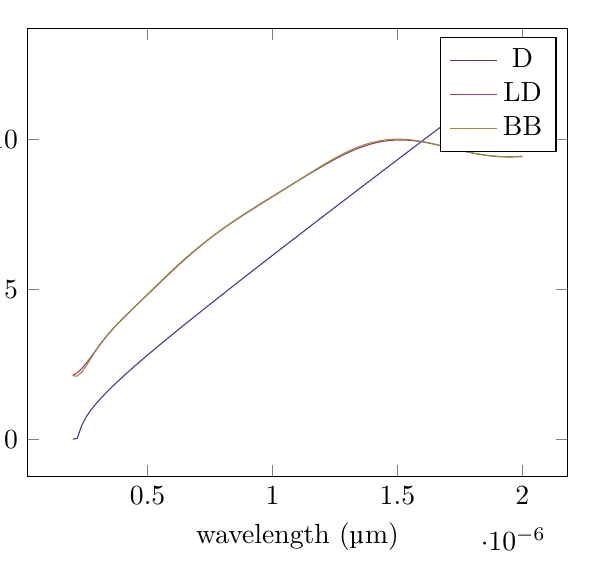
\begin{tikzpicture}[baseline,trim axis left]
\begin{axis}[xlabel=wavelength (\si{\micro\meter}),ylabel=$n''$]
\addplot[color=colora] coordinates {
(2e-07, 0.0161231270038)
(2.18181818182e-07, 0.0411379708636)
(2.36363636364e-07, 0.476265524818)
(2.54545454545e-07, 0.762756888978)
(2.72727272727e-07, 0.981580085134)
(2.90909090909e-07, 1.1711478415)
(3.09090909091e-07, 1.34387746274)
(3.27272727273e-07, 1.50556881589)
(3.45454545455e-07, 1.65944814055)
(3.63636363636e-07, 1.80750927978)
(3.81818181818e-07, 1.95107523762)
(4e-07, 2.09107028214)
(4.18181818182e-07, 2.22816589798)
(4.36363636364e-07, 2.36286519501)
(4.54545454545e-07, 2.49555465081)
(4.72727272727e-07, 2.62653733715)
(4.90909090909e-07, 2.75605508274)
(5.09090909091e-07, 2.88430373179)
(5.27272727273e-07, 3.01144393509)
(5.45454545455e-07, 3.13760895929)
(5.63636363636e-07, 3.2629104525)
(5.81818181818e-07, 3.38744277641)
(6e-07, 3.51128631209)
(6.18181818182e-07, 3.63451001773)
(6.36363636364e-07, 3.75717343228)
(6.54545454545e-07, 3.87932826267)
(6.72727272727e-07, 4.00101965388)
(6.90909090909e-07, 4.12228721483)
(7.09090909091e-07, 4.24316585384)
(7.27272727273e-07, 4.36368646453)
(7.45454545455e-07, 4.48387649288)
(7.63636363636e-07, 4.60376040915)
(7.81818181818e-07, 4.72336010307)
(8e-07, 4.84269521672)
(8.18181818182e-07, 4.96178342635)
(8.36363636364e-07, 5.08064068223)
(8.54545454545e-07, 5.19928141371)
(8.72727272727e-07, 5.31771870535)
(8.90909090909e-07, 5.43596444877)
(9.09090909091e-07, 5.55402947412)
(9.27272727273e-07, 5.67192366439)
(9.45454545455e-07, 5.78965605498)
(9.63636363636e-07, 5.90723492092)
(9.81818181818e-07, 6.02466785337)
(1e-06, 6.14196182697)
(1.01818181818e-06, 6.25912325937)
(1.03636363636e-06, 6.3761580638)
(1.05454545455e-06, 6.49307169586)
(1.07272727273e-06, 6.60986919513)
(1.09090909091e-06, 6.72655522219)
(1.10909090909e-06, 6.84313409188)
(1.12727272727e-06, 6.95960980294)
(1.14545454545e-06, 7.07598606472)
(1.16363636364e-06, 7.19226632121)
(1.18181818182e-06, 7.30845377264)
(1.2e-06, 7.42455139505)
(1.21818181818e-06, 7.54056195796)
(1.23636363636e-06, 7.65648804042)
(1.25454545455e-06, 7.77233204551)
(1.27272727273e-06, 7.88809621364)
(1.29090909091e-06, 8.00378263455)
(1.30909090909e-06, 8.11939325833)
(1.32727272727e-06, 8.23492990543)
(1.34545454545e-06, 8.3503942759)
(1.36363636364e-06, 8.46578795773)
(1.38181818182e-06, 8.58111243466)
(1.4e-06, 8.69636909317)
(1.41818181818e-06, 8.81155922907)
(1.43636363636e-06, 8.92668405349)
(1.45454545455e-06, 9.04174469837)
(1.47272727273e-06, 9.15674222163)
(1.49090909091e-06, 9.27167761183)
(1.50909090909e-06, 9.38655179256)
(1.52727272727e-06, 9.50136562648)
(1.54545454545e-06, 9.61611991905)
(1.56363636364e-06, 9.73081542201)
(1.58181818182e-06, 9.84545283661)
(1.6e-06, 9.96003281659)
(1.61818181818e-06, 10.074555971)
(1.63636363636e-06, 10.1890228667)
(1.65454545455e-06, 10.303434031)
(1.67272727273e-06, 10.4177899537)
(1.69090909091e-06, 10.5320910891)
(1.70909090909e-06, 10.6463378585)
(1.72727272727e-06, 10.7605306513)
(1.74545454545e-06, 10.8746698274)
(1.76363636364e-06, 10.9887557184)
(1.78181818182e-06, 11.1027886291)
(1.8e-06, 11.2167688393)
(1.81818181818e-06, 11.3306966047)
(1.83636363636e-06, 11.4445721583)
(1.85454545455e-06, 11.5583957117)
(1.87272727273e-06, 11.6721674562)
(1.89090909091e-06, 11.7858875635)
(1.90909090909e-06, 11.8995561871)
(1.92727272727e-06, 12.0131734631)
(1.94545454545e-06, 12.1267395107)
(1.96363636364e-06, 12.2402544338)
(1.98181818182e-06, 12.353718321)
(2e-06, 12.4671312467)
};
\addlegendentry{D}
\addplot[color=colorb] coordinates {
(2e-07, 2.14407339974)
(2.18181818182e-07, 2.2269465826)
(2.36363636364e-07, 2.36839243773)
(2.54545454545e-07, 2.54920914685)
(2.72727272727e-07, 2.75071710011)
(2.90909090909e-07, 2.95829261848)
(3.09090909091e-07, 3.16230540581)
(3.27272727273e-07, 3.35743994989)
(3.45454545455e-07, 3.54156405716)
(3.63636363636e-07, 3.71469445055)
(3.81818181818e-07, 3.87816851868)
(4e-07, 4.03399708795)
(4.18181818182e-07, 4.18437178095)
(4.36363636364e-07, 4.33131704602)
(4.54545454545e-07, 4.47647861425)
(4.72727272727e-07, 4.62103069838)
(4.90909090909e-07, 4.76567429105)
(5.09090909091e-07, 4.91069477139)
(5.27272727273e-07, 5.05604949276)
(5.45454545455e-07, 5.20146275136)
(5.63636363636e-07, 5.34651354867)
(5.81818181818e-07, 5.49070868324)
(6e-07, 5.63353891636)
(6.18181818182e-07, 5.77451914138)
(6.36363636364e-07, 5.91321503321)
(6.54545454545e-07, 6.04925909644)
(6.72727272727e-07, 6.1823588476)
(6.90909090909e-07, 6.31229940764)
(7.09090909091e-07, 6.43894225797)
(7.27272727273e-07, 6.56222143884)
(7.45454545455e-07, 6.68213808556)
(7.63636363636e-07, 6.79875391099)
(7.81818181818e-07, 6.91218404096)
(8e-07, 7.02258947302)
(8.18181818182e-07, 7.13016934161)
(8.36363636364e-07, 7.2351531182)
(8.54545454545e-07, 7.33779284226)
(8.72727272727e-07, 7.43835545947)
(8.90909090909e-07, 7.53711533164)
(9.09090909091e-07, 7.63434697575)
(9.27272727273e-07, 7.73031808387)
(9.45454545455e-07, 7.82528287211)
(9.63636363636e-07, 7.91947580381)
(9.81818181818e-07, 8.01310572996)
(1e-06, 8.10635048867)
(1.01818181818e-06, 8.19935200593)
(1.03636363636e-06, 8.29221194067)
(1.05454545455e-06, 8.38498791981)
(1.07272727273e-06, 8.47769041242)
(1.09090909091e-06, 8.57028029657)
(1.10909090909e-06, 8.66266717723)
(1.12727272727e-06, 8.75470851869)
(1.14545454545e-06, 8.84620965943)
(1.16363636364e-06, 8.93692478059)
(1.18181818182e-06, 9.02655889993)
(1.2e-06, 9.11477096038)
(1.21818181818e-06, 9.20117807481)
(1.23636363636e-06, 9.28536097385)
(1.25454545455e-06, 9.36687068143)
(1.27272727273e-06, 9.44523641031)
(1.29090909091e-06, 9.51997462769)
(1.30909090909e-06, 9.59059918777)
(1.32727272727e-06, 9.65663236659)
(1.34545454545e-06, 9.71761656559)
(1.36363636364e-06, 9.77312638019)
(1.38181818182e-06, 9.82278066299)
(1.4e-06, 9.8662541558)
(1.41818181818e-06, 9.90328822845)
(1.43636363636e-06, 9.93370025212)
(1.45454545455e-06, 9.95739115678)
(1.47272727273e-06, 9.97435077951)
(1.49090909091e-06, 9.98466070137)
(1.50909090909e-06, 9.98849439129)
(1.52727272727e-06, 9.98611461614)
(1.54545454545e-06, 9.97786822544)
(1.56363636364e-06, 9.96417856301)
(1.58181818182e-06, 9.94553588342)
(1.6e-06, 9.92248624584)
(1.61818181818e-06, 9.89561941609)
(1.63636363636e-06, 9.86555632423)
(1.65454545455e-06, 9.83293660311)
(1.67272727273e-06, 9.79840667714)
(1.69090909091e-06, 9.76260878996)
(1.70909090909e-06, 9.72617126359)
(1.72727272727e-06, 9.68970018014)
(1.74545454545e-06, 9.65377258036)
(1.76363636364e-06, 9.61893118548)
(1.78181818182e-06, 9.58568057787)
(1.8e-06, 9.55448472081)
(1.81818181818e-06, 9.52576566135)
(1.83636363636e-06, 9.49990323925)
(1.85454545455e-06, 9.47723561849)
(1.87272727273e-06, 9.45806046247)
(1.89090909091e-06, 9.44263658638)
(1.90909090909e-06, 9.43118593879)
(1.92727272727e-06, 9.42389578517)
(1.94545454545e-06, 9.42092098868)
(1.96363636364e-06, 9.42238630531)
(1.98181818182e-06, 9.42838863081)
(2e-06, 9.43899915526)
};
\addlegendentry{LD}
\addplot[color=colorc] coordinates {
(2e-07, 2.12996715473)
(2.18181818182e-07, 2.11681797791)
(2.36363636364e-07, 2.24578137213)
(2.54545454545e-07, 2.46133068762)
(2.72727272727e-07, 2.70695600068)
(2.90909090909e-07, 2.94729269569)
(3.09090909091e-07, 3.16817542302)
(3.27272727273e-07, 3.36759450764)
(3.45454545455e-07, 3.54868265312)
(3.63636363636e-07, 3.71604599913)
(3.81818181818e-07, 3.87412507997)
(4e-07, 4.0265657572)
(4.18181818182e-07, 4.17606431214)
(4.36363636364e-07, 4.32442554178)
(4.54545454545e-07, 4.47270630237)
(4.72727272727e-07, 4.62138159399)
(4.90909090909e-07, 4.77050265453)
(5.09090909091e-07, 4.91983347784)
(5.27272727273e-07, 5.06896134437)
(5.45454545455e-07, 5.21738189665)
(5.63636363636e-07, 5.36456175413)
(5.81818181818e-07, 5.50998260873)
(6e-07, 5.65317078956)
(6.18181818182e-07, 5.79371585084)
(6.36363636364e-07, 5.93128110609)
(6.54545454545e-07, 6.06560837715)
(6.72727272727e-07, 6.19651864541)
(6.90909090909e-07, 6.32390982209)
(7.09090909091e-07, 6.44775249847)
(7.27272727273e-07, 6.56808428268)
(7.45454545455e-07, 6.68500315489)
(7.63636363636e-07, 6.79866015674)
(7.81818181818e-07, 6.90925169674)
(8e-07, 7.0170114103)
(8.18181818182e-07, 7.12220235284)
(8.36363636364e-07, 7.22510882119)
(8.54545454545e-07, 7.32602852835)
(8.72727272727e-07, 7.42526496619)
(8.90909090909e-07, 7.52312006184)
(9.09090909091e-07, 7.61988717553)
(9.27272727273e-07, 7.71584447404)
(9.45454545455e-07, 7.81124870344)
(9.63636363636e-07, 7.90632937791)
(9.81818181818e-07, 8.00128339832)
(1e-06, 8.09627011558)
(1.01818181818e-06, 8.19140685818)
(1.03636363636e-06, 8.28676495205)
(1.05454545455e-06, 8.382366272)
(1.07272727273e-06, 8.47818037833)
(1.09090909091e-06, 8.57412230748)
(1.10909090909e-06, 8.67005110301)
(1.12727272727e-06, 8.76576918883)
(1.14545454545e-06, 8.86102270149)
(1.16363636364e-06, 8.95550290869)
(1.18181818182e-06, 9.04884884505)
(1.2e-06, 9.14065129081)
(1.21818181818e-06, 9.23045820154)
(1.23636363636e-06, 9.3177816638)
(1.25454545455e-06, 9.40210640158)
(1.27272727273e-06, 9.48289979061)
(1.29090909091e-06, 9.55962325312)
(1.30909090909e-06, 9.63174480952)
(1.32727272727e-06, 9.69875246167)
(1.34545454545e-06, 9.76016798555)
(1.36363636364e-06, 9.81556062862)
(1.38181818182e-06, 9.86456015251)
(1.4e-06, 9.90686864234)
(1.41818181818e-06, 9.94227052789)
(1.43636363636e-06, 9.97064033041)
(1.45454545455e-06, 9.99194775753)
(1.47272727273e-06, 10.0062599102)
(1.49090909091e-06, 10.0137405261)
(1.50909090909e-06, 10.0146463472)
(1.52727272727e-06, 10.0093208556)
(1.54545454545e-06, 9.99818574782)
(1.56363636364e-06, 9.98173061706)
(1.58181818182e-06, 9.96050136759)
(1.6e-06, 9.93508790448)
(1.61818181818e-06, 9.90611162145)
(1.63636363636e-06, 9.87421316074)
(1.65454545455e-06, 9.84004084717)
(1.67272727273e-06, 9.80424011327)
(1.69090909091e-06, 9.76744414212)
(1.70909090909e-06, 9.73026586636)
(1.72727272727e-06, 9.69329138112)
(1.74545454545e-06, 9.65707475955)
(1.76363636364e-06, 9.6221342037)
(1.78181818182e-06, 9.5889494225)
(1.8e-06, 9.55796010011)
(1.81818181818e-06, 9.52956530282)
(1.83636363636e-06, 9.50412366711)
(1.85454545455e-06, 9.48195421482)
(1.87272727273e-06, 9.46333765052)
(1.89090909091e-06, 9.44851801009)
(1.90909090909e-06, 9.43770454563)
(1.92727272727e-06, 9.43107374944)
(1.94545454545e-06, 9.42877143749)
(1.96363636364e-06, 9.43091482971)
(1.98181818182e-06, 9.43759458036)
(2e-06, 9.4488767255)
};
\addlegendentry{BB}
\end{axis}
\end{tikzpicture}%
\\
\end{tabular}
\caption{Material parameters for Pt based on the Drude, Lorentz-Drude, and Brendel-Bormann models.}
\end{figure}
\clearpage


%%%%% Part I - Overview
%\chapter{Overview}
%\label{ch:overview}
%Biosensors based on surface plasmon resonance play a central role as a
simple and remarkably responsive label-free method for characterizing and
quantifying biomolecular
interactions~\cite{homola1999surface}~\cite{homola2006surface}.  Amongst
the most popular of these sensors are those which excite localized surface
plasmon polaritons on thin metal films in prism coupled
configurations~\cite{hoa2007towards}.  These platforms, despite their
ubiquity and commercial success, are host to an amazing depth of useful
phenomena which has yet to be explored in the context of biosensing.  In
particular, the nature of 

Herein is described investigations of single and multiply scattered surface
plasmon polaritons from such a system.  Specifically, we look at the
structure of the re-radiated optical field which contain additional
features such as near field self-interference, speckle, and optical
vorticies, and their relations to the scattering microstructure.  Our
results suggest several possible avenues for advancing the detection limits
of surface plasmon based biosensors for both single particles and bulk
refractive index measurements.

A photon is a quantized oscillation of an electromagnetic field.  When an
electromagnetic  field is in proximity to an interface such as the surface
of a metal, oscillations of free charge can be induced.  If the field is
evanescent in both directions orthogonal to the surface, the oscillations
become localized and are known as surface plasmons (SPs).  Furthermore, if
conditions exist such that the in-plane momentum and phase of an incident
photon and the surface plasmon match, the coupling produces a hybrid
excitation known as surface plasmon polariton (SPP).  An SPP is trapped on
the interface and propagates until it decays; either re-radiating as a
photon or being absorbed into the metal as heat.

SPPs, like photons, are quantum mechanical objects.  Given system is
momentum-conserving, elastically scattered plasmons will preserve all the
information of their parent field.  

In the literature one will find a sense of interchangability regarding
the terms ``plasmon'', ``surface plasmon'', ``localized surface plasmon'',
and ``surface plasmon polariton''.  To be clear, in this work we are always
refering to surface plasmon \textit{polaritons}: a surface plasmon which is
strongly coupled to the exciting electromagnetic field.  SPPs are a type of
quasiparticle, as they are essentially a collective excitation of free
electrons.  The fundamental point here is that strong coupling preserves
quantum mechanical information.

\subsection{Organization}
This work is roughly organized in the following way.
\Chapter{ch:existence} is what you are currently reading.  Here is laid out
theory, mathematical details regarding the conditions under which SPPs may
be excited, and physical properties.  In \Chapter{ch:experimental} we
describe all details regarding the physical experiment: construction,
protocols, , and data analysis.  These first two chapters form the
mathematical and physical basis for the remaining text.

Discussion of our studies and new results begins with \Chapter{ch:bulkri}.
Here, the bulk refractive index sensing properties of the cone are
described.  Closely related, \Chapter{ch:interference} discusses a newly
discovered interference phenomena in the cone and the possible utility in
the context of SPR refractive index sensing.

Perhaps one of the most interesting features of the cone is speckle, the
subject of \Chapter{ch:speckle}.  Here we compare the properties of cone
speckle with those of classic speckle fields in the context of
correlations, refractive index pertrubations, and multiple scattering
effects.

Finally, in \Chapter{ch:scatteringmicro} we look at the influence of the
cone speckle on the scattering microstructure itself.

%\section{Historical Perspective}
%\label{sec:review}
%The theoretical groundwork for the existence of surface plasmon polaritons
(SPPs) was first introduced by Richie in his seminal 1957 paper
\textit{Plasma Losses by Fast Electrons in Thin Films}
\cite{ritchie1957plasma}.  Like any scientific work, Richie's was
incremental and has its roots in earlier theoretical proposals by Pines and
Bohm~\cite{bohm1951collective}~\cite{pines1952collective}.  Ultimately this
research functioned to explain the phenomena of sharp and spectrally narrow
energy losses observed in diffraction gratings by Wood in 1902, known as
``Wood's anomaly''.

Optical excitation of surface plasmons was made accessible through
pioneering work in the late 1960's by Kretschmann~\cite{kretschmann1968},
Raether~\cite{raether1965springer} and Otto~\cite{otto1968excitation}.
These experiments used the principle of attenuated total reflection (ATR) to
excite surface plasmons evanescently, using a prism to match their
resonance condition.  A great deal of understanding on the topic of surface
plasmons took place in the subsequent decade, such as an improved
theoretical understanding based on Fresnel relations
\cite{chen1976excitation} and descriptions of of conically scattered light
in the presence of surface roughness~\cite{simon1976directional}.  A
concise overview of this research can be found in
\cite{raether1997surface}.

The introduction of SPR as a biosensing platform began in the early 1980's
with work by Liedberg, Nylander and Lundstrom~\cite{liedberg1983surface}
who described the extraordinary sensitivity of the surface plasmon
resonance condition to perturbations in the refractive index of the medium
on one side of the film.  The subsequent commercialization of SPR
biosensors has largely been influenced by these authors and Pharmacia
Biosensor AB (now Biacore)~\cite{liedberg1995biosensing}.

The commercial success of biosensors based on surface plasmon resonance
seems to have brought about a knowledge gap between the biosensing
community and their more theoretical predecessors from whom the field owes
its genesis.  This is to say that the scope of SPR biosensing experiments
is disproportionately narrower than the breadth of phenomena discovered
since Richie.  As an example particular to this minithesis, in 2005 and
2007, two papers~\cite{andaloro2005optical}~\cite{simon2007observation}
based on theoretical work by Chuang~\cite{chuang1986lateral} and Chen
\cite{chen1976excitation} reported a curious interference pattern occurring
in the specularly reflected light for certain (among them,
Kretschmann-Raether type) systems illuminated with focused Gaussian beams.
This was also independently reported a year later in
\cite{schumann2008near}.  Interestingly, observation of this interference
required nothing more than the addition of a lens pair to a fairly
ubiquitous optical setup, but it somehow escaped attention during earlier
research.  In this thesis, we have observed the same phenomena, but by
considering conically scattered light have arrived on a different
description as to its origin.

Many of the topics here are influenced by a 2009 thesis {\it Surface
Plasmon Random Scattering and Related Phenomena}
\cite{schumann2009surface} by Schumann.  Here, the author describes
experiments performed on thin metal films in a Kretschmann-Raether
configuration with the addition of a scanning of an apertureless near-field
probe.  This probe (a sharp tungsten tip) is able to elastically scatter
SPPs in a way analogous to surface roughness, but in this case its location
and interaction can be precisely controlled.  By observing the way light is
scattered relative to the position of the probe it is possible to, among
other things, modify the resonance condition in-situ.

%\section{Plane Wave Solutions to Maxwell's Equations}
%Conditions for the existence and excitation of SPPs can be completely
predicted from Maxwell's equations.  We begin with their derivation here,
starting with the differential form of Maxwell's
equations~\cite{maier2007plasmonics}~\cite{benson2009elements} including
external sources.
\begin{align}
\nabla \cdot \mathbf{D} &= \rho & \text{Gauss's law} \label{eqn:gausslaw}\\
\nabla \cdot \mathbf{B} &= 0 & \text{Gauss's law for magnetism} \label{eqn:gausslawmagnetism}\\
\nabla \times \mathbf{E} &= -\frac{\partial \mathbf{B}} {\partial t}
& \text{Faraday's law of induction} \label{eqn:faradayslaw} \\
\nabla \times \mathbf{H} &= \frac{\partial \mathbf{D}} {\partial
t} + \mathbf{J}  & \text{Ampere's law with Maxwell's correction}
\label{eqn:ampereslaw}
\end{align}
where $\mathbf{E}$ is the electric field, $\mathbf{B}$ is the magnetic
field, $\mathbf{D}$ is the electric displacement field with an external
charge density $\rho$, and $\mathbf{H}$ is the auxiliary magnetic field
with current density $\mathbf{J}$.

In formulating Maxwell's equations it is assumed all electromagnetic
propagation takes place in a {\it simple dielectric}, that is
\begin{enumerate}
\item The polarization density $\mathbf{P}$ is linear with the electric
field $\mathbf{E}$.  
\begin{align}
\mathbf{P}=\epsilon_0\chi_e\mathbf{E}
\label{eqn:pdensity}
\end{align}
where $\chi_e$ is the electric susceptibility.  From this and the definition
of $\mathbf{D}$
\begin{align}
\mathbf{D}=\epsilon_0\mathbf{E}+\mathbf{P}
\label{eqn:dfield}
\end{align},
where $\epsilon_0$ is the permittivity of free space, one can simplify the
$\mathbf{D}$-field as 
\begin{align}
\mathbf{D}&=\epsilon_0\mathbf{E}+\mathbf{P}\\
%&=\epsilon_0 \mathbf{E}+\epsilon_0 \chi_e \mathbf{E}\\
&=\epsilon_0(1+\chi_e)\mathbf{E}\\
&=\epsilon\mathbf{E}
\end{align}
Here $\epsilon$ has been defined to be the permittivity of the
dielectric.  The convention in this work is usually that variables with a
subscript $0$ can always be assumed to be that variable {\it in vacuo},
while their material dependent counterparts have no subscript.
\item The magnetization $\mathbf{M}$, related to the auxiliary magnetic
field by is linear in $\mathbf{H}$
\begin{align}
\mathbf{M}=\mu_0\chi_m\mathbf{H}
\end{align}
where $\chi_m$ is the volume magnetic susceptibility.  This allows the
magnetic field to be rewritten according to its definition
\begin{align}
\mathbf{B}&=\mu_0\left(\mathbf{H}+\mathbf{M}\right)\\
&=\mu_0\left(1+\chi_m\right)\mathbf{H}\\
&=\mu \mathbf{H}
\end{align}
where $\mu_0$ is the vacuum permeability of free space.  In practice, most
dielectrics have nearly zero magnetic response, so $\mathbf{M}=0$ and
$\mu_0=\mu$ is a valid assumption.  Nevertheless, for the sake of generality it is treated as a
material dependent parameter.
\item The material is homogeneous and isotropic.
\item Charge is conserved.  $\mathbf{J} = \sigma \mathbf{E}$, where
 $\sigma$ is the conductivity and
\begin{align}
 \frac{\partial \rho}{\partial t} 
  &= -\nabla \cdot \mathbf{J}\\
  &= -\sigma \left(\nabla \cdot \mathbf{E} \right) \\
  &= -\frac{\sigma}{\epsilon} \rho
\end{align}
\end{enumerate}

%\section{Dispersion Relation}
%With plane wave solutions in hand, boundary conditions consistent with a
single interface can be imposed.
At a planar interface, it is convenient to restrict the problem to TM
polarization in two
dimensions; in this case the $x$-$z$. Since $\mathbf{k}=(k_x,0,k_z)$,
$\mathbf{r}\cdot\mathbf{k}=k_x x + k_z z$ and $\mathbf{E}_0 = (E_x, 0,
E_z)$, the electric field can be written 
\begin{align}
\mathbf{E} ( \mathbf{r}, t ) &= \mathbf{E}_0\, \me^{\mi (\mathbf{k}
\cdot \mathbf{r} - \omega t )}\\
\mathbf{E}(x,z,t)&=\begin{pmatrix}
E_x\\ 0\\ E_z
\end{pmatrix}
\, \me^{\mi(k_{x,i}x+k_{z,i}z-\omega t)}
\label{eqn:planewavexz}
\end{align}
The magnetic field propagates in the same direction with the
same $\mathbf{k}$-vector components, but the direction
$\mathbf{H}$ must be orthogonal to $\mathbf{E}$ by
\Equation{eqn:faradayslaw}
\begin{align}
\mathbf{H} ( \mathbf{r}, t ) &= \mathbf{H}_0\, \me^{\mi (\mathbf{k}
\cdot \mathbf{r} - \omega t )}\\
\mathbf{H}(x,z,t)&=\begin{pmatrix}
0\\ H_y\\ 0
\end{pmatrix}
\, \me^{\mi(k_{x,i}x+k_{z,i}z-\omega t)}
\end{align}
At the interface there are two values for the (complex) permittivity,
$\epsilon_1$ and $\epsilon_2$.  Consequently
there are two sets of plane wave solutions
\begin{align}
\left.\begin{aligned}
\mathbf{H}_1(x,z,t) &=
\begin{pmatrix}
0\\
H_{y,1}\\
0
\end{pmatrix} \me^{\mi(k_{x,1}x+k_{z,1}z-\omega t)}\\
\mathbf{E}_1(x,z,t) &=
\begin{pmatrix}
E_{x,1}\\
0\\
E_{z,1}\\
\end{pmatrix} \me^{\mi(k_{x,1}x+k_{z,1}z-\omega t)}
\end{aligned}
\right\}& \quad \epsilon_1\label{eqn:planewavedielectric}\\
\left.\begin{aligned}
\mathbf{H}_2(x,z,t) &=
\begin{pmatrix}
0\\
H_{y,2}\\
0
\end{pmatrix}
\me^{\mi(k_{x,2}x+k_{z,2}z-\omega t)}\\
\mathbf{E}_2(x,z,t) &=
\begin{pmatrix}
E_{x,2}\\
0\\
E_{z,2}\\
\end{pmatrix}
\me^{\mi(k_{x,2}x+k_{z,2}z-\omega t)}
\end{aligned} 
\right\}&\quad \epsilon_2
\label{eqn:planewavemetal}
\end{align}
where the subscript designates which material the wave equation refers to.
(e.g. $\mathbf{E}_1$ is the electric field in $\epsilon_1$, $\mathbf{H}_2$
the magnetic field in the $\epsilon_2$, etc.)
Continuity of \Equation{eqn:planewavedielectric} and
\ref{eqn:planewavemetal} at this interface requires that
\begin{align}
E_{x,2}&=E_{x,1}\\
H_{y,2}&=H_{y,1}\\
\epsilon_2 E_{z,2}&=\epsilon_1 E_{z,1}
\end{align}
Applying Ampere's law (\Equation{eqn:ampereslaw}) to the field on the
each boundary gives
\begin{align}
\nabla \times \mathbf{H}_i &= \epsilon_i \frac{\partial \mathbf{E}_i}{\partial t}\\
\begin{pmatrix}
\frac{\partial H_{z,i}}{\partial y} - \frac{\partial H_{y,i}}{\partial z}\\
\frac{\partial H_{x,i}}{\partial y} - \frac{\partial H_{z,i}}{\partial z}\\
\frac{\partial H_{y,i}}{\partial y} - \frac{\partial H_{x,i}}{\partial z}
\end{pmatrix}
&= \begin{pmatrix}
-\mi k_{z,i} H_{y,i}\\
0\\
\mi k_{x,i} H_{y,i}
\end{pmatrix}
\\
&= \begin{pmatrix}
-\mi \omega \epsilon_i E_{x,i}\\
0\\
-\mi \omega \epsilon_i E_{z,i}
\end{pmatrix}
\label{eqn:vectordisp}
\end{align}
where $\mathbf{E}_i$, $\mathbf{H}_i$, $i=1,2$ represent the field in either the
$\epsilon_1$ or $\epsilon_2$.  The vector components of
\Equation{eqn:vectordisp} are therefore related 
\begin{align}
-\mi k_{z,i} H_{y,i} &= -\mi \omega \epsilon_i E_{x,i}\\
k_{z,1} H_{y,1} &= \omega \epsilon_1 E_{x,1}\\
k_{z,2} H_{y,2} &= \omega \epsilon_2 E_{x,2}
\label{eqn:spderivsteptwo}
\end{align}
Since the components of both $\mathbf{E}_i$ and $\mathbf{H}_i$ are
parallel to the interface, $E_{x,i}$ and $H_{y,i}$ are also
continuous. By substitution of $E_{x,i}$, \Equation{eqn:spderivsteptwo} becomes
\begin{align}
\frac{k_{z,1}}{\epsilon_1}H_{y,1}&=\frac{k_{z,2}}{\epsilon_2}H_{y,2}\\ 
\Aboxed{
\frac{k_{z,1}}{\epsilon_1}&=\frac{k_{z,2}}{\epsilon_2} 
}
\label{eqn:sprcondition}
\end{align}
This is the surface plasmon resonance condition.  Note an important aspect
of \Equation{eqn:sprcondition}.  Due to the way we have defined our
geometry, $k_{z,1}$ must be postive and $k_{z,2}$ negative.  For
\Equation{eqn:sprcondition} to hold, this implies that the real part of
$\epsilon_1$ and $\epsilon_2$ are opposite in sign.  For materials we know
exist, this is fulfilled if $\epsilon_1$ is a dielectric and $\epsilon_2$
is a metal.

\section{Dispersion Relation}
In terms of its vector components, the following holds in general for all
electromagnetic waves
\begin{align}
\mathbf{k}^2=\epsilon_i \left(\frac{\omega}{c}\right)^2=k_x^2 + k_{z,i}^2\\
\epsilon_i k_0^2=k_x^2 + k_{z,i}^2
\label{eqn:dispersion1}
\end{align}
Substitution of \Equation{eqn:sprcondition} with the relation 
$k_{x,1}=k_{x,2}$ into \Equation{eqn:dispersion1} allows 
$k_x$ and $k_{z,i}$ to be rewritten in the form of a dispersion relation
\begin{align}
k_x &= k_0\sqrt{\frac{\epsilon_1 \epsilon_2}{\epsilon_1+\epsilon_2}} 
= \frac{\omega}{c}\sqrt{\frac{\epsilon_1 \epsilon_2}{\epsilon_1+\epsilon_2}}\\
k_{z,i} &= k_0\frac{\epsilon_i}{\sqrt{\epsilon_1+\epsilon_2}}
= \frac{\omega}{c}\frac{\epsilon_i}{\sqrt{\epsilon_1+\epsilon_2}}
\end{align}

This relation, shown in \Figure{fig:dispersionrelation}, is useful because
it shows graphically the condition under which SPPs may exist: at the
intersection between the photon light line and corresponding SPP light line
for the medium in question.  Note that for a photon and a plasmon in both a
vacuum and a dielectric, this never happens; the photon assumes $\omega = c
k /\sqrt{\epsilon_i}$ for $i=1,2$, diverging to infinity while the SPP
asymptotically approaches $\omega_p/\sqrt{1+\epsilon_i}$ as $k_x\to\infty$.
However, if light is incident from a dielectric $\epsilon_1$ at an angle
$\theta$, the slope of $\omega(k_x)$ is modified to $c k \sin
\theta/\sqrt{\epsilon_1}$ and the dispersion relations can be matched.
This is the principle exploited by Kretschmann \cite{kretschmann1968} to
excite SPPs with prisms.

There are several regions of interest in \Figure{fig:dispersionrelation},
depending on the relative value of $\epsilon_1$ and $\epsilon_2$.  We first
assume that $\epsilon_1$ is a dielectric with $\epsilon_1\in\mathbb{R}$ and
$\epsilon_1 > 0$ (true for most if not all glass).  In this case, for
$\Re(\epsilon_2)>0$, both $k_x$ and $k_z$ are real.  These are known as
``radiative modes'' -- an SPP mode is supported normal to the interface but
it is not bound there.  For $-\epsilon_1<\Re(\epsilon_2)<0$, $k_z$ is real
and $k_x$ imaginary.  The SPP is not confined to the interface and decays
evanescently there; this is known as a ``quasi-bound mode''  However, for
$\Re(\epsilon_2)<-\epsilon_1$, $k_x$ is real and $k_z$ is imaginary.  This
indicates the SPP is localized at the interface in $z$ while having a
propagating solution in $x$, and is exactly the condition we wish to match.
\import{existence/figures/}{dispersionfig}

%\subsection{Spatial Extension of the SPP Field}
%\input{dispersion/spatial}
%\subsection{Resonance Condition}
%\input{dispersion/resonance}
%\section{Fresnel Relations}
%Much of the behavior of SPR in prism coupled configurations can be
succinctly expressed in terms of the Fresnel relations with complex
permittivities.  For TM polarization they are

\begin{align}
 \tilde{r}_{j,l,m \ldots n}(k_x) = 
\frac{\tilde{r}_{j,l} + \tilde{r}_{l,m \ldots n} \me^{2 \mi k_{z,l} d_l}}
{1+\tilde{r}_{j,l} \tilde{r}_{l,m \ldots n} \me^{2 \mi k_{z,l} d_l}}
\label{eqn:bertnlayer}
\end{align}
where $d_l$ is the thickness of the $l$th metal layer and 
\begin{align}
\tilde{r}_{i,j}&=\frac{\epsilon_j k_{z,i}-\epsilon_i k_{z,j}}
{\epsilon_j k_{z,i}+\epsilon_i k_{z,j}}
\end{align}
is the two layer Fresnel relation.  \Equation{eqn:bertnlayer} may be
recursively applied for any number of layers.

In this equation, $k_{z,i}$ can be equivalently expressed either as a
function of incident angle $\theta$ or $k_x$
\begin{align}
k_{z,i} &= k_0 \sqrt{\epsilon_i - \epsilon_1 \sin \theta}\\
&= \sqrt{k_0^2\epsilon_i - k_x^2}
\end{align}


%\section{The Fourier Optics Perspective of SPR}
%\input{perspective}
%% z propagation distances
\renewcommand{\fresnelpropzA}{$z=\SI{0.05}{\milli\meter}$}
\renewcommand{\fresnelpropzB}{$z=\SI{0.25}{\milli\meter}$}
\renewcommand{\fresnelpropzC}{$z=\SI{0.5}{\milli\meter}$}
\renewcommand{\fresnelpropzD}{$z=\SI{1.0}{\milli\meter}$}
\renewcommand{\fresnelpropzE}{$z=\SI{2.5}{\milli\meter}$}
\renewcommand{\fresnelpropzF}{$z=\SI{5.0}{\milli\meter}$}
\renewcommand{\fresnelpropzG}{$z=\SI{10.0}{\milli\meter}$}
\renewcommand{\fresnelpropzH}{$z=\SI{50.0}{\milli\meter}$}

% base directory
\renewcommand{\fresnelpropbasedir}{wigglespropagate/bk7-au-h2o-633}

\begin{figure}[ht]
\centering
\pgfplotsset{
 minor tick num=3,
 small,
 every axis/.style={thick,width=0.56\textwidth,height=0.20\textwidth},
 legend style={ legend pos = north east, font = \small, draw = none},
}
\begin{tabular}{ll}
\multicolumn{1}{c}{\large \centering $|E_\text{spec}|^2$ }
&\multicolumn{1}{c}{\large \centering $|E_\text{cone}|^2$ }\\
\begin{tikzpicture}[baseline,trim axis left]
\begin{axis}
\addlegendimage{empty legend}
\addlegendentry{\fresnelpropzA}
\addplot[color=colora] file {\fresnelpropbasedir/fresnelpropzAspec.dat};
\addplot[color=colorb,dashed] file {\fresnelpropbasedir/fresnelpropzAgauss.dat};
\end{axis}
\end{tikzpicture}%
&
\begin{tikzpicture}[baseline,trim axis left]
\begin{axis}
\addlegendimage{empty legend}
\addlegendentry{\fresnelpropzA}
\addplot[color=colorc] file {\fresnelpropbasedir/fresnelpropzAcone.dat};
\end{axis}
\end{tikzpicture}%
\\
\begin{tikzpicture}[baseline,trim axis left]
\begin{axis}
\addlegendimage{empty legend}
\addlegendentry{\fresnelpropzB}
\addplot[color=colora] file {\fresnelpropbasedir/fresnelpropzBspec.dat};
\addplot[color=colorb,dashed] file {\fresnelpropbasedir/fresnelpropzBgauss.dat};
\end{axis}
\end{tikzpicture}%
&
\begin{tikzpicture}[baseline,trim axis left]
\begin{axis}
\addlegendimage{empty legend}
\addlegendentry{\fresnelpropzB}
\addplot[color=colorc] file {\fresnelpropbasedir/fresnelpropzBcone.dat};
\end{axis}
\end{tikzpicture}%
\\
\begin{tikzpicture}[baseline,trim axis left]
\begin{axis}
\addlegendimage{empty legend}
\addlegendentry{\fresnelpropzC}
\addplot[color=colora] file {\fresnelpropbasedir/fresnelpropzCspec.dat};
\addplot[color=colorb,dashed] file {\fresnelpropbasedir/fresnelpropzCgauss.dat};
\end{axis}
\end{tikzpicture}%
&
\begin{tikzpicture}[baseline,trim axis left]
\begin{axis}
\addlegendimage{empty legend}
\addlegendentry{\fresnelpropzC}
\addplot[color=colorc] file {\fresnelpropbasedir/fresnelpropzCcone.dat};
\end{axis}
\end{tikzpicture}%
\\
\begin{tikzpicture}[baseline,trim axis left]
\begin{axis}
\addlegendimage{empty legend}
\addlegendentry{\fresnelpropzD}
\addplot[color=colora] file {\fresnelpropbasedir/fresnelpropzDspec.dat};
\addplot[color=colorb,dashed] file {\fresnelpropbasedir/fresnelpropzDgauss.dat};
\end{axis}
\end{tikzpicture}%
&
\begin{tikzpicture}[baseline,trim axis left]
\begin{axis}
\addlegendimage{empty legend}
\addlegendentry{\fresnelpropzD}
\addplot[color=colorc] file {\fresnelpropbasedir/fresnelpropzDcone.dat};
\end{axis}
\end{tikzpicture}%
\\
\begin{tikzpicture}[baseline,trim axis left]
\begin{axis}
\addlegendimage{empty legend}
\addlegendentry{\fresnelpropzE}
\addplot[color=colora] file {\fresnelpropbasedir/fresnelpropzEspec.dat};
\addplot[color=colorb,dashed] file {\fresnelpropbasedir/fresnelpropzEgauss.dat};
\end{axis}
\end{tikzpicture}%
&
\begin{tikzpicture}[baseline,trim axis left]
\begin{axis}
\addlegendimage{empty legend}
\addlegendentry{\fresnelpropzE}
\addplot[color=colorc] file {\fresnelpropbasedir/fresnelpropzEcone.dat};
\end{axis}
\end{tikzpicture}%
\\
\begin{tikzpicture}[baseline,trim axis left]
\begin{axis}
\addlegendimage{empty legend}
\addlegendentry{\fresnelpropzF}
\addplot[color=colora] file {\fresnelpropbasedir/fresnelpropzFspec.dat};
\addplot[color=colorb,dashed] file {\fresnelpropbasedir/fresnelpropzFgauss.dat};
\end{axis}
\end{tikzpicture}%
&
\begin{tikzpicture}[baseline,trim axis left]
\begin{axis}
\addlegendimage{empty legend}
\addlegendentry{\fresnelpropzF}
\addplot[color=colorc] file {\fresnelpropbasedir/fresnelpropzFcone.dat};
\end{axis}
\end{tikzpicture}%
\\
\begin{tikzpicture}[baseline,trim axis left]
\begin{axis}
\addlegendimage{empty legend}
\addlegendentry{\fresnelpropzG}
\addplot[color=colora] file {\fresnelpropbasedir/fresnelpropzGspec.dat};
\addplot[color=colorb,dashed] file {\fresnelpropbasedir/fresnelpropzGgauss.dat};
\end{axis}
\end{tikzpicture}%
&
\begin{tikzpicture}[baseline,trim axis left]
\begin{axis}
\addlegendimage{empty legend}
\addlegendentry{\fresnelpropzG}
\addplot[color=colorc] file {\fresnelpropbasedir/fresnelpropzGcone.dat};
\end{axis}
\end{tikzpicture}%
\\
\begin{tikzpicture}[baseline,trim axis left]
\begin{axis}[
xlabel=detector scale,
/pgfplots/change x base,
/pgfplots/x unit=\si{\micro\meter},
]
\addlegendimage{empty legend}
\addlegendentry{\fresnelpropzH}
\addplot[color=colora] file {\fresnelpropbasedir/fresnelpropzHspec.dat};
\addplot[color=colorb,dashed] file {\fresnelpropbasedir/fresnelpropzHgauss.dat};
\end{axis}
\end{tikzpicture}%
&
\begin{tikzpicture}[baseline,trim axis left]
\begin{axis}[
xlabel=detector scale,
/pgfplots/change x base,
/pgfplots/x unit=\si{\micro\meter},
]
\addlegendimage{empty legend}
\addlegendentry{\fresnelpropzH}
\addplot[color=colorc] file {\fresnelpropbasedir/fresnelpropzHcone.dat};
%\addplot[color=colorc,mark=x,mark size={0.750},only marks] file {data/farfield-cone-mod.txt};
\end{axis}
\end{tikzpicture}%
\end{tabular}
\caption{Simulated $|E_\text{spec}(x,z)|^2$ and $|E_\text{cone}(x,z)|^2$
for different propagation distances $z$.  The incident Gaussian beam
$\tilde{g}(k_x)$ has been propagated unmodified by the Fresnel term and
appears alongside $|E_\text{spec}(x,z)|^2$ as a dashed line.}
\label{fig:fresnelpropagate}
\end{figure}

%%%\section{Interrogation Methods}
%%%Thus far we have not found a way to use this phenomena to enhance
measurements of bulk refractive index sensitivity in SPR\@.  The responses in
the near field track well as the field propagates into the far field.
There is a possibility that the additional structure in the spatial
oscillations may help fitting routines, but we have not investigated this
rigorously.
%What you should do here is the following: use MRF's code to make near field
%x-z plots of system A and system B.  Then take the difference between the
%two.  If there is any better way that will let you know.
%It is also possible to make some plots using the original dango wiggles
%code.

%%%Intensity, angular, wavelength

%% Part III - My Progress
%\chapter{Summary of Progress}
%\label{ch:summary}
%\input{summary}
%\section{Datasets}
%\input{theoretical}
%\section{Experiment}
%\input{experiment/experiment}
%\section{One Sided Oscillations in Reflected and Scattered Light}
%\input{experiment/spdiscussion}
%\section{Bulk Index Sensitivity}
%\input{experiment/sens}
%\section{Miscellaneous}
%\subsection{High Dynamic Range Imaging}
%\input{hdr/hdr}
%\subsection{Microfluidics}
%Microfluidic flow cells made of polydimethylsiloxane (PDMS) were used to
introduce analytes into the sensing volume.  PDMS is a bio-compatible
organosilicon compound obtained as a two part elastomer kit\footnote{Dow
Corning Sylgard\textregistered 184}.  The two part liquid is combined in a
10:1 ratio by mass in a small plastic mixing cup.  The correct proportions
are determined by an analytical balance to a precision of \SI{0.01}{\gram}.
They are then combined and mixed using a magnetic stir paddle for
\SI{5}{\minute}.  The mixture is poured on to a polished silicon wafer in a
shallow glass dish and evacuated in a vacuum bell jar until all dissolved
gas has been removed.  The PDMS is then baked for \SI{20}{\minute} at
\SI{120}{\celsius}.  Once removed, the cured PDMS is cut free from the mold
using a scalpel and transferred to a clean glass slide where it is stored
in a dust free environment until use.

The PDMS is cast into \SI{1}{\milli\meter} thick layers which were cut into
\SI{25x25}{\milli\meter} squares.  Horizontally embedded and centered in the
PDMS layer layer was a length of \SI{0.6}{\milli\meter} outside diameter
silicone tubing.  A circular biopsy punch was used to extract a
\SI{6}{\milli\meter} hole from the center, which cut the tubing in its center.
The hypotenuse of the prism with its complete layer substructure was then
placed over the remaining side of the central hole; the surface attraction
between the PDMS and the prism substrate was sufficient to prevent leakage.  A
siphon was set up between the input and output channels in the PDMS and the
experiment run with a flow rate of \SI{1.85}{\micro\liter\per\second}.  The
microfluidic flow cell as integrated into the experiment is shown schematically
in \Figure{fig:microfluidiccell}.

As a cursory note, when handling PDMS or anything PDMS comes into contact
with, a clean pair of nitrile gloves should be used.  It was observed that
surfaces which had been touched with powder-free latex gloves could no
longer be directly bonded.  The present anecdote seems to be prevalent in
the literature, but no description of the underlying mechanism is known.

\begin{figure}[ht]
\centering
\import{experimental/figures/}{microfluidics.pdf_tex}
\caption{Schematic of the microfluidic cell as integrated in the experiment.}
\label{fig:microfluidiccell}
\end{figure}

%\subsection{Probe Tips}
%\input{tip/tip}
%
%%%% Part IV - Future Research
%\chapter{Future Research}
%\label{ch:future}
%\input{future/future}

%\bibliographystyle{plain}
%\bibliography{imprs_minithesis}

% publication list
% acknowlegements
%%\appendix
%%\section{Physical Properties of SPP Propagation at a Metal-Air Interface at $\lambda_0=\SI{632.8}{\nano\meter}$}
%%\label{sec:spptable}
%%\sisetup{
  round-mode = figures,
  round-precision = 8,
}%
\begin{table}
\begin{tabularx}{\textwidth}{lllllll}
\toprule
metal& model& permittivity & $\lambda_\text{sp}$ & $1/(2 k_x)$ & $1/k_{z,2}$ & $1/k_{z,1}$ \\
\midrule
\multirow{3}{*}{Ag}
 &LD&\num{-14.482393640216667308+1.0945548544552969883i}&\num{610.69773663262276386}&\num{17445.210431591880479}&\num{25.519442863192477233}&\num{370.71458834326284659}\\
 &D&\num{-16.858544219836005595+0.43750947302633563796i}&\num{613.75881925148655682}&\num{59734.457234373221581}&\num{23.788479449446406022}&\num{401.1826703205257445}\\
 &BB&\num{-14.450239807763432864+1.1928708187898817705i}&\num{610.67374412141373341}&\num{15951.923119463852345}&\num{25.542790547775389598}&\num{370.44792616582236633}\\
\midrule
\multirow{3}{*}{Au}
 &LD&\num{-9.8001417660154466205+1.9648780045450582321i}&\num{601.0685993758610266}&\num{4387.3400605935721615}&\num{30.374436198256290709}&\num{304.25559309440831157}\\
 &D&\num{-15.131388920027497136+0.43636288213944929293i}&\num{611.55136993383507615}&\num{47737.089113776841259}&\num{25.018551523178910401}&\num{378.73394864922698844}\\
 &BB&\num{-10.564933676629095771+1.2740573715299496893i}&\num{602.59332443152845826}&\num{7729.3254599240390235}&\num{29.441776470583967296}&\num{313.53764804208157102}\\
\midrule
\multirow{3}{*}{Cu}
 &LD&\num{-12.39652684258414439+2.4145493333716290252i}&\num{607.77370876765940011}&\num{5893.7230323202229556}&\num{27.323572914174345527}&\num{345.6295617380971521}\\
 &D&\num{-16.563994453718034805+0.26893338361912622059i}&\num{613.40642406135293641}&\num{93612.063746043175342}&\num{23.986659270826407919}&\num{397.3706194157928735}\\
 &BB&\num{-11.70283381729212735+2.1037740651380825163i}&\num{606.10434335299294162}&\num{5946.5877325303854377}&\num{28.065616318072532209}&\num{334.19513542113918447}\\
\midrule
\multirow{3}{*}{Al}
 &LD&\num{-51.48940819368333166+19.557449805308333879i}&\num{627.41696143280944398}&\num{15226.507322391251364}&\num{13.671516084348438014}&\num{753.91489062846869729}\\
 &D&\num{-29.554544896388971864+0.73294915303824959008i}&\num{622.00911748623684616}&\num{114056.22880846841144}&\num{18.208284353173350922}&\num{538.30881110289635672}\\
 &BB&\num{-51.407135782086868403+18.436833640456043781i}&\num{627.33225436078737403}&\num{15873.827245506914551}&\num{13.705678672394880024}&\num{749.33123952527591882}\\
\midrule
\multirow{3}{*}{Be}
 &LD&\num{1.6713774473717268876+21.837379481280162707i}&\num{634.3904514695693706}&\num{2226.6292793784859896}&\num{30.988049927934955718}&\num{712.7303600025193191}\\
 &D&\num{-6.494693887412333666+0.1338819760077697707i}&\num{582.07366944362013328}&\num{24705.734415409708163}&\num{36.348566343216319297}&\num{236.13208964935373047}\\
 &BB&\num{1.4494223885240540284+21.656671587538273371i}&\num{634.27146693823908663}&\num{2203.8901308072377105}&\num{30.96211516677081832}&\num{705.77365106241688864}\\
\midrule
\multirow{3}{*}{Cr}
 &LD&\num{-7.0181432300565189664+29.847831042912378763i}&\num{630.675468165340817}&\num{3138.8179062659523879}&\num{22.835981399376482415}&\num{718.15732865899315129}\\
 &D&\num{-4.0544826952447978741+0.12124804421367750551i}&\num{549.34688013146376306}&\num{8941.0965896332618286}&\num{43.412899725174497689}&\num{176.12128173395578301}\\
 &BB&\num{-7.170752602123531716+28.466736537581464717i}&\num{630.42385835625429991}&\num{3013.0091036700250697}&\num{23.177307042108409973}&\num{698.28307893071871604}\\
\midrule
\multirow{3}{*}{Ni}
 &LD&\num{-9.5076370076869984871+14.842248819650812663i}&\num{623.60924060260538226}&\num{2015.2194703714492334}&\num{26.58766134382839752}&\num{481.44049250964468456}\\
 &D&\num{-5.3342780374432354762+0.15518099415325858903i}&\num{570.47512337973842023}&\num{13541.529440339487337}&\num{39.305372567281068541}&\num{209.77494050588956043}\\
 &BB&\num{-9.4712322187005710816+14.848816865610180216i}&\num{623.63348865181751535}&\num{2011.3378735881044577}&\num{26.611947383455149208}&\num{481.55105903433747017}\\
\midrule
\multirow{3}{*}{Pd}
 &LD&\num{-14.242110714627109758+15.286524853996523277i}&\num{622.69699161360051676}&\num{2738.5717348955276975}&\num{23.460428084586474995}&\num{497.93639994455264741}\\
 &D&\num{-7.1215620995403678961+0.033161160941418882375i}&\num{586.69289759753382896}&\num{122757.9927918798785}&\num{34.989824803824241428}&\num{249.18535291312448976}\\
 &BB&\num{-14.313594990707592558+15.284643849211908773i}&\num{622.68920649745234641}&\num{2751.2693811245462712}&\num{23.422021103950680043}&\num{498.18595509035344548}\\
\midrule
\multirow{3}{*}{Pt}
 &LD&\num{-11.949432860425986291+19.298242480668985621i}&\num{625.76328314622980997}&\num{2598.1598808500057203}&\num{23.675349826526652208}&\num{548.98662536810934398}\\
 &D&\num{-6.9644968954448591703+0.32519847799012108203i}&\num{585.73021145994505332}&\num{11938.332869812194986}&\num{35.311409468769738851}&\num{246.23901538208389184}\\
 &BB&\num{-12.039470923577166417+19.390875327601026612i}&\num{625.78546132916460465}&\num{2614.8775107829683293}&\num{23.604599280395760275}&\num{550.29719415469321575}\\
\midrule
\multirow{3}{*}{Ti}
 &LD&\num{-5.8179384262032662889+12.945914643794955268i}&\num{624.61761205315667667}&\num{1503.8533991419162703}&\num{30.769871373152462013}&\num{455.80554060965914687}\\
 &D&\num{-1.0453002872560821501+0.085599475134401012411i}&\num{219.25753180835766898}&\num{31.849444863765626224}&\num{33.355927731132887004}&\num{36.586356972153630807}\\
 &BB&\num{-5.651775038402902851+12.898779928522792204i}&\num{624.76468214401450041}&\num{1486.9156150929773048}&\num{30.977773742769436183}&\num{455.74341532091557383}\\
\midrule
\multirow{3}{*}{W}
 &LD&\num{5.1796609248482425869+21.23181642531190505i}&\num{636.68311757849744481}&\num{2305.3247826714855364}&\num{34.138264152482221903}&\num{789.0326579240808087}\\
 &D&\num{-8.3684410835066138645+0.30601835334898985774i}&\num{593.84806743198214463}&\num{19073.47903514835707}&\num{32.664872935955443722}&\num{273.56154797160900216}\\
 &BB&\num{5.4200719219360706802+20.345820585128890912i}&\num{637.14691471286880642}&\num{2237.750478645799376}&\num{35.229112486378092228}&\num{786.83191845447663582}\\
\midrule
\bottomrule
\end{tabularx}
\begin{tabularx}{\textwidth}{ll}
\toprule
\multicolumn{2}{l}{Table Abbreviations}\\
\midrule
metal & atomic symbol for the metal \\
model & theoretical model: D $\mapsto$ Drude, LD $\mapsto$ Lorentz-Drude, BB $\mapsto$ Brendel-Bormann \\
permittivity & complex permittivity $\epsilon$, in farads per meter \\
$\lambda_\text{sp}$ & SPP wavelength normal to the interface, in nanometers\\
$1/k_x$ & $1/\me$ SPP propagation distance normal to the interface, in nanometers \\
$1/k_{z,2}$ & $1/\me$ distance of evanescent decay into the metal, in nanometers \\
$1/k_{z,1}$ & $1/\me$ distance of evanescent decay into air, in nanometers \\
\bottomrule
\end{tabularx}
\caption{Physical properties of a vacuum-metal interface for various metals at
$\lambda_0=\SI{632.8}{\nano\meter}$. }%
\label{tbl:sptable_632}
\end{table}

%%\section{Material Parameters for Metal Films}
%%\label{sec:drudemetals}
%%The following figures plot the frequency-dependent complex permittivity
$\epsilon = \epsilon' + \mi \epsilon''$ and refractive index $n = n' + \mi
n''$ for silver, aluminum, gold, copper, chromium, nickel, tungsten,
titanium, beryllium, palladium, and platinum using either the Drude
(\Equation{eqn:drude}),
Lorentz-Drude (\Equation{eqn:lorentzdrude}), or Brendel-Bormann
(\Equation{eqn:brendelbormann})  models in the range
\SIrange{200}{2000}{\nano\meter}.  The material parameters and mathematical
formalism detailed in~\cite{rakic1998optical}.  These tables are generated
programmatically.
Three different models for the complex permittivity are tabulated.  The
first two are the Drude and Lorentz-Drude (LD) models.
\begin{align}
\epsilon_{D}&=\epsilon_D\\
\epsilon_{LD}&=\epsilon_D+\epsilon_L
\end{align}
where $\epsilon_D$ is contribution from the Drude model, representing
free electron effects
\begin{align}
\epsilon_D=1-\frac{\sqrt{f_0} \omega_p^{\prime 2}}{\omega(\omega -
\mi\Gamma_0^\prime)}
\label{eqn:drude}
\end{align}
and $\epsilon_L$ is the Lorentz contribution, representing the bound
electron effects
\begin{align}
\epsilon_L =\sum_{j=0}^{k}\frac{f_j\omega_p^{\prime 2}}{\omega_j^{\prime
2}-\omega^2+\mi\omega\Gamma_j^\prime}
\label{eqn:lorentzdrude}
\end{align}
The third is the Brendel-Bormann model which is based instead on an
infinite superposition of oscillators
\begin{align}
\epsilon_\text{BB} = \frac{1}{\sqrt{2 \pi} \sigma_n} \intinfty
\exp\left(-\frac{(x-\omega'_n)}{2 \sigma_n^2}\right)
\frac{f_j \omega_p^2}{(x^2-\omega^2)+\mi \omega \Gamma'_n} \md x
\label{eqn:brendelbormann}
\end{align}
\newpage
\pgfplotsset{%
 minor tick num=3,
 small,
 every axis/.style={thick,width=\textwidth,height=0.35\textwidth,legend columns=3},
}
\newpage
\subsection{Ag}
\begin{figure}[h!]
\centering
\begin{tabular}{l}
\begin{tikzpicture}[baseline,trim axis left]
\begin{axis}[xlabel=wavelength (\si{\micro\meter}),ylabel=permittivity $\epsilon'$]
\addplot[color=colora] coordinates {%
(2e-07, -0.78487418047)
(2.18181818182e-07, -1.12412357997)
(2.36363636364e-07, -1.49286415804)
(2.54545454545e-07, -1.89109372276)
(2.72727272727e-07, -2.318809907)
(2.90909090909e-07, -2.77601016848)
(3.09090909091e-07, -3.26269178977)
(3.27272727273e-07, -3.77885187838)
(3.45454545455e-07, -4.32448736675)
(3.63636363636e-07, -4.89959501234)
(3.81818181818e-07, -5.50417139763)
(4e-07, -6.13821293024)
(4.18181818182e-07, -6.8017158429)
(4.36363636364e-07, -7.49467619358)
(4.54545454545e-07, -8.21708986551)
(4.72727272727e-07, -8.96895256725)
(4.90909090909e-07, -9.75025983273)
(5.09090909091e-07, -10.5610070214)
(5.27272727273e-07, -11.4011893181)
(5.45454545455e-07, -12.2708017335)
(5.63636363636e-07, -13.1698391036)
(5.81818181818e-07, -14.0982960906)
(6e-07, -15.0561671821)
(6.18181818182e-07, -16.0434466919)
(6.36363636364e-07, -17.0601287597)
(6.54545454545e-07, -18.1062073511)
(6.72727272727e-07, -19.1816762582)
(6.90909090909e-07, -20.2865290992)
(7.09090909091e-07, -21.4207593186)
(7.27272727273e-07, -22.5843601874)
(7.45454545455e-07, -23.7773248032)
(7.63636363636e-07, -24.9996460903)
(7.81818181818e-07, -26.2513167996)
(8e-07, -27.532329509)
(8.18181818182e-07, -28.8426766233)
(8.36363636364e-07, -30.1823503745)
(8.54545454545e-07, -31.5513428216)
(8.72727272727e-07, -32.9496458512)
(8.90909090909e-07, -34.3772511772)
(9.09090909091e-07, -35.8341503409)
(9.27272727273e-07, -37.3203347117)
(9.45454545455e-07, -38.8357954863)
(9.63636363636e-07, -40.3805236899)
(9.81818181818e-07, -41.9545101754)
(1e-06, -43.5577456239)
(1.01818181818e-06, -45.1902205452)
(1.03636363636e-06, -46.8519252773)
(1.05454545455e-06, -48.5428499868)
(1.07272727273e-06, -50.2629846694)
(1.09090909091e-06, -52.0123191493)
(1.10909090909e-06, -53.7908430802)
(1.12727272727e-06, -55.5985459448)
(1.14545454545e-06, -57.4354170551)
(1.16363636364e-06, -59.3014455529)
(1.18181818182e-06, -61.1966204096)
(1.2e-06, -63.1209304264)
(1.21818181818e-06, -65.0743642346)
(1.23636363636e-06, -67.0569102956)
(1.25454545455e-06, -69.0685569014)
(1.27272727273e-06, -71.1092921742)
(1.29090909091e-06, -73.1791040674)
(1.30909090909e-06, -75.2779803647)
(1.32727272727e-06, -77.4059086814)
(1.34545454545e-06, -79.5628764638)
(1.36363636364e-06, -81.7488709896)
(1.38181818182e-06, -83.9638793683)
(1.4e-06, -86.2078885411)
(1.41818181818e-06, -88.4808852813)
(1.43636363636e-06, -90.7828561942)
(1.45454545455e-06, -93.1137877177)
(1.47272727273e-06, -95.4736661223)
(1.49090909091e-06, -97.8624775112)
(1.50909090909e-06, -100.280207821)
(1.52727272727e-06, -102.72684282)
(1.54545454545e-06, -105.202368112)
(1.56363636364e-06, -107.706769134)
(1.58181818182e-06, -110.240031155)
(1.6e-06, -112.802139281)
(1.61818181818e-06, -115.393078449)
(1.63636363636e-06, -118.012833434)
(1.65454545455e-06, -120.661388842)
(1.67272727273e-06, -123.338729117)
(1.69090909091e-06, -126.044838536)
(1.70909090909e-06, -128.779701214)
(1.72727272727e-06, -131.543301099)
(1.74545454545e-06, -134.335621976)
(1.76363636364e-06, -137.156647466)
(1.78181818182e-06, -140.006361026)
(1.8e-06, -142.884745951)
(1.81818181818e-06, -145.791785371)
(1.83636363636e-06, -148.727462254)
(1.85454545455e-06, -151.691759405)
(1.87272727273e-06, -154.684659466)
(1.89090909091e-06, -157.70614492)
(1.90909090909e-06, -160.756198083)
(1.92727272727e-06, -163.834801113)
(1.94545454545e-06, -166.941936005)
(1.96363636364e-06, -170.077584594)
(1.98181818182e-06, -173.241728554)
(2e-06, -176.434349397)
};
\addlegendentry{D}
\addplot[color=colorb] coordinates {%
(2e-07, 1.35905059416)
(2.18181818182e-07, 0.550331143561)
(2.36363636364e-07, -0.401215462349)
(2.54545454545e-07, -1.69666894637)
(2.72727272727e-07, -1.47353407777)
(2.90909090909e-07, 1.91584883134)
(3.09090909091e-07, 0.858580330628)
(3.27272727273e-07, -0.176281144322)
(3.45454545455e-07, -1.03861711603)
(3.63636363636e-07, -1.82120810677)
(3.81818181818e-07, -2.57181745556)
(4e-07, -3.31432340551)
(4.18181818182e-07, -4.06164464627)
(4.36363636364e-07, -4.82132528813)
(4.54545454545e-07, -5.59805997105)
(4.72727272727e-07, -6.39492566494)
(4.90909090909e-07, -7.2140267208)
(5.09090909091e-07, -8.05685394607)
(5.27272727273e-07, -8.9244951388)
(5.45454545455e-07, -9.81776410752)
(5.63636363636e-07, -10.7372827926)
(5.81818181818e-07, -11.6835352791)
(6e-07, -12.656904353)
(6.18181818182e-07, -13.6576968733)
(6.36363636364e-07, -14.6861617783)
(6.54545454545e-07, -15.7425031216)
(6.72727272727e-07, -16.8268896787)
(6.90909090909e-07, -17.939462142)
(7.09090909091e-07, -19.0803385877)
(7.27272727273e-07, -20.249618686)
(7.45454545455e-07, -21.4473869825)
(7.63636363636e-07, -22.6737154835)
(7.81818181818e-07, -23.9286657153)
(8e-07, -25.212290378)
(8.18181818182e-07, -26.5246346866)
(8.36363636364e-07, -27.8657374669)
(8.54545454545e-07, -29.235632057)
(8.72727272727e-07, -30.6343470547)
(8.90909090909e-07, -32.0619069413)
(9.09090909091e-07, -33.5183326047)
(9.27272727273e-07, -35.0036417802)
(9.45454545455e-07, -36.5178494255)
(9.63636363636e-07, -38.0609680398)
(9.81818181818e-07, -39.6330079361)
(1e-06, -41.2339774773)
(1.01818181818e-06, -42.8638832778)
(1.03636363636e-06, -44.5227303801)
(1.05454545455e-06, -46.210522407)
(1.07272727273e-06, -47.9272616954)
(1.09090909091e-06, -49.6729494128)
(1.10909090909e-06, -51.4475856597)
(1.12727272727e-06, -53.2511695602)
(1.14545454545e-06, -55.0836993415)
(1.16363636364e-06, -56.9451724046)
(1.18181818182e-06, -58.8355853867)
(1.2e-06, -60.7549342174)
(1.21818181818e-06, -62.7032141678)
(1.23636363636e-06, -64.6804198954)
(1.25454545455e-06, -66.6865454836)
(1.27272727273e-06, -68.7215844776)
(1.29090909091e-06, -70.7855299162)
(1.30909090909e-06, -72.8783743611)
(1.32727272727e-06, -75.0001099226)
(1.34545454545e-06, -77.1507282834)
(1.36363636364e-06, -79.3302207196)
(1.38181818182e-06, -81.5385781207)
(1.4e-06, -83.7757910066)
(1.41818181818e-06, -86.0418495437)
(1.43636363636e-06, -88.3367435597)
(1.45454545455e-06, -90.6604625566)
(1.47272727273e-06, -93.0129957231)
(1.49090909091e-06, -95.3943319455)
(1.50909090909e-06, -97.8044598181)
(1.52727272727e-06, -100.243367652)
(1.54545454545e-06, -102.711043485)
(1.56363636364e-06, -105.207475087)
(1.58181818182e-06, -107.732649969)
(1.6e-06, -110.286555393)
(1.61818181818e-06, -112.869178369)
(1.63636363636e-06, -115.480505671)
(1.65454545455e-06, -118.120523835)
(1.67272727273e-06, -120.789219169)
(1.69090909091e-06, -123.486577753)
(1.70909090909e-06, -126.212585446)
(1.72727272727e-06, -128.967227891)
(1.74545454545e-06, -131.750490514)
(1.76363636364e-06, -134.562358531)
(1.78181818182e-06, -137.402816952)
(1.8e-06, -140.271850581)
(1.81818181818e-06, -143.169444021)
(1.83636363636e-06, -146.095581674)
(1.85454545455e-06, -149.050247748)
(1.87272727273e-06, -152.033426252)
(1.89090909091e-06, -155.045101007)
(1.90909090909e-06, -158.08525564)
(1.92727272727e-06, -161.153873592)
(1.94545454545e-06, -164.250938115)
(1.96363636364e-06, -167.376432278)
(1.98181818182e-06, -170.530338963)
(2e-06, -173.712640872)
};
\addlegendentry{LD}
\addplot[color=colorc] coordinates {%
(2e-07, -0.247217875147)
(2.18181818182e-07, -0.741091026792)
(2.36363636364e-07, -0.693905648861)
(2.54545454545e-07, -0.863316785951)
(2.72727272727e-07, -1.57071009976)
(2.90909090909e-07, 0.779270341698)
(3.09090909091e-07, 1.11053219674)
(3.27272727273e-07, -0.23106368434)
(3.45454545455e-07, -1.24507591502)
(3.63636363636e-07, -2.07675287028)
(3.81818181818e-07, -2.84682061258)
(4e-07, -3.5938063176)
(4.18181818182e-07, -4.33565854094)
(4.36363636364e-07, -5.08287579503)
(4.54545454545e-07, -5.84215676472)
(4.72727272727e-07, -6.61795868206)
(4.90909090909e-07, -7.41333250166)
(5.09090909091e-07, -8.23041702509)
(5.27272727273e-07, -9.07074472552)
(5.45454545455e-07, -9.93543609128)
(5.63636363636e-07, -10.8253257289)
(5.81818181818e-07, -11.7410458102)
(6e-07, -12.6830823777)
(6.18181818182e-07, -13.6518140768)
(6.36363636364e-07, -14.6475393019)
(6.54545454545e-07, -15.6704955671)
(6.72727272727e-07, -16.7208735619)
(6.90909090909e-07, -17.7988275102)
(7.09090909091e-07, -18.9044829163)
(7.27272727273e-07, -20.0379424321)
(7.45454545455e-07, -21.1992903549)
(7.63636363636e-07, -22.3885961138)
(7.81818181818e-07, -23.6059169982)
(8e-07, -24.8513003126)
(8.18181818182e-07, -26.1247850934)
(8.36363636364e-07, -27.4264034856)
(8.54545454545e-07, -28.7561818559)
(8.72727272727e-07, -30.1141416975)
(8.90909090909e-07, -31.5003003706)
(9.09090909091e-07, -32.9146717116)
(9.27272727273e-07, -34.3572665368)
(9.45454545455e-07, -35.8280930609)
(9.63636363636e-07, -37.3271572465)
(9.81818181818e-07, -38.8544630973)
(1e-06, -40.4100129045)
(1.01818181818e-06, -41.993807455)
(1.03636363636e-06, -43.605846209)
(1.05454545455e-06, -45.2461274494)
(1.07272727273e-06, -46.9146484111)
(1.09090909091e-06, -48.6114053908)
(1.10909090909e-06, -50.3363938415)
(1.12727272727e-06, -52.089608454)
(1.14545454545e-06, -53.8710432278)
(1.16363636364e-06, -55.6806915316)
(1.18181818182e-06, -57.5185461564)
(1.2e-06, -59.3845993622)
(1.21818181818e-06, -61.2788429178)
(1.23636363636e-06, -63.2012681364)
(1.25454545455e-06, -65.1518659066)
(1.27272727273e-06, -67.1306267195)
(1.29090909091e-06, -69.1375406927)
(1.30909090909e-06, -71.1725975915)
(1.32727272727e-06, -73.235786848)
(1.34545454545e-06, -75.3270975771)
(1.36363636364e-06, -77.4465185918)
(1.38181818182e-06, -79.5940384162)
(1.4e-06, -81.769645297)
(1.41818181818e-06, -83.9733272142)
(1.43636363636e-06, -86.2050718906)
(1.45454545455e-06, -88.4648668)
(1.47272727273e-06, -90.7526991747)
(1.49090909091e-06, -93.0685560124)
(1.50909090909e-06, -95.4124240826)
(1.52727272727e-06, -97.7842899316)
(1.54545454545e-06, -100.184139888)
(1.56363636364e-06, -102.611960067)
(1.58181818182e-06, -105.067736374)
(1.6e-06, -107.551454511)
(1.61818181818e-06, -110.063099975)
(1.63636363636e-06, -112.602658066)
(1.65454545455e-06, -115.170113887)
(1.67272727273e-06, -117.765452349)
(1.69090909091e-06, -120.388658171)
(1.70909090909e-06, -123.039715882)
(1.72727272727e-06, -125.718609827)
(1.74545454545e-06, -128.425324163)
(1.76363636364e-06, -131.159842866)
(1.78181818182e-06, -133.922149729)
(1.8e-06, -136.712228368)
(1.81818181818e-06, -139.530062216)
(1.83636363636e-06, -142.375634531)
(1.85454545455e-06, -145.248928396)
(1.87272727273e-06, -148.149926716)
(1.89090909091e-06, -151.078612225)
(1.90909090909e-06, -154.034967482)
(1.92727272727e-06, -157.018974875)
(1.94545454545e-06, -160.030616622)
(1.96363636364e-06, -163.069874768)
(1.98181818182e-06, -166.13673119)
(2e-06, -169.231167598)
};
\addlegendentry{BB}
\end{axis}
\end{tikzpicture}%
\\
\begin{tikzpicture}[baseline,trim axis left]
\begin{axis}[xlabel=wavelength (\si{\micro\meter}),ylabel=permittivity $\epsilon''$]
\addplot[color=colora] coordinates {%
(2e-07, 0.0138201424947)
(2.18181818182e-07, 0.0179420992488)
(2.36363636364e-07, 0.0228115184097)
(2.54545454545e-07, 0.0284906550796)
(2.72727272727e-07, 0.0350417563395)
(2.90909090909e-07, 0.0425270606326)
(3.09090909091e-07, 0.0510087971485)
(3.27272727273e-07, 0.060549185207)
(3.45454545455e-07, 0.0712104336428)
(3.63636363636e-07, 0.0830547401899)
(3.81818181818e-07, 0.0961442908663)
(4e-07, 0.110541259359)
(4.18181818182e-07, 0.126307806411)
(4.36363636364e-07, 0.143506079203)
(4.54545454545e-07, 0.162198210743)
(4.72727272727e-07, 0.18244631925)
(4.90909090909e-07, 0.204312507544)
(5.09090909091e-07, 0.227858862427)
(5.27272727273e-07, 0.253147454075)
(5.45454545455e-07, 0.280240335424)
(5.63636363636e-07, 0.309199541558)
(5.81818181818e-07, 0.340087089095)
(6e-07, 0.372964975578)
(6.18181818182e-07, 0.407895178866)
(6.36363636364e-07, 0.444939656516)
(6.54545454545e-07, 0.484160345182)
(6.72727272727e-07, 0.525619159998)
(6.90909090909e-07, 0.569377993971)
(7.09090909091e-07, 0.615498717375)
(7.27272727273e-07, 0.664043177138)
(7.45454545455e-07, 0.715073196237)
(7.63636363636e-07, 0.768650573089)
(7.81818181818e-07, 0.824837080947)
(8e-07, 0.883694467288)
(8.18181818182e-07, 0.945284453214)
(8.36363636364e-07, 1.00966873284)
(8.54545454545e-07, 1.0769089727)
(8.72727272727e-07, 1.14706681112)
(8.90909090909e-07, 1.22020385765)
(9.09090909091e-07, 1.29638169242)
(9.27272727273e-07, 1.37566186558)
(9.45454545455e-07, 1.45810589666)
(9.63636363636e-07, 1.54377527398)
(9.81818181818e-07, 1.63273145409)
(1e-06, 1.72503586109)
(1.01818181818e-06, 1.8207498861)
(1.03636363636e-06, 1.91993488664)
(1.05454545455e-06, 2.02265218603)
(1.07272727273e-06, 2.12896307277)
(1.09090909091e-06, 2.2389288)
(1.10909090909e-06, 2.35261058484)
(1.12727272727e-06, 2.47006960784)
(1.14545454545e-06, 2.59136701239)
(1.16363636364e-06, 2.71656390406)
(1.18181818182e-06, 2.84572135011)
(1.2e-06, 2.97890037881)
(1.21818181818e-06, 3.11616197889)
(1.23636363636e-06, 3.25756709894)
(1.25454545455e-06, 3.40317664684)
(1.27272727273e-06, 3.55305148913)
(1.29090909091e-06, 3.70725245046)
(1.30909090909e-06, 3.865840313)
(1.32727272727e-06, 4.02887581582)
(1.34545454545e-06, 4.19641965436)
(1.36363636364e-06, 4.36853247978)
(1.38181818182e-06, 4.54527489844)
(1.4e-06, 4.72670747129)
(1.41818181818e-06, 4.91289071326)
(1.43636363636e-06, 5.10388509273)
(1.45454545455e-06, 5.29975103093)
(1.47272727273e-06, 5.50054890136)
(1.49090909091e-06, 5.70633902919)
(1.50909090909e-06, 5.91718169073)
(1.52727272727e-06, 6.13313711282)
(1.54545454545e-06, 6.35426547227)
(1.56363636364e-06, 6.58062689528)
(1.58181818182e-06, 6.81228145686)
(1.6e-06, 7.04928918029)
(1.61818181818e-06, 7.2917100365)
(1.63636363636e-06, 7.53960394356)
(1.65454545455e-06, 7.79303076604)
(1.67272727273e-06, 8.05205031453)
(1.69090909091e-06, 8.31672234499)
(1.70909090909e-06, 8.58710655823)
(1.72727272727e-06, 8.86326259936)
(1.74545454545e-06, 9.14525005717)
(1.76363636364e-06, 9.43312846363)
(1.78181818182e-06, 9.7269572933)
(1.8e-06, 10.0267959628)
(1.81818181818e-06, 10.3327038301)
(1.83636363636e-06, 10.6447401943)
(1.85454545455e-06, 10.9629642946)
(1.87272727273e-06, 11.2874353104)
(1.89090909091e-06, 11.6182123599)
(1.90909090909e-06, 11.9553545003)
(1.92727272727e-06, 12.2989207269)
(1.94545454545e-06, 12.6489699725)
(1.96363636364e-06, 13.0055611071)
(1.98181818182e-06, 13.3687529372)
(2e-06, 13.738604205)
};
\addlegendentry{D}
\addplot[color=colorb] coordinates {%
(2e-07, 0.404835204104)
(2.18181818182e-07, 0.445563994275)
(2.36363636364e-07, 0.656396239051)
(2.54545454545e-07, 1.48626855057)
(2.72727272727e-07, 4.80154843687)
(2.90909090909e-07, 2.9158733781)
(3.09090909091e-07, 1.25770688622)
(3.27272727273e-07, 0.812670594646)
(3.45454545455e-07, 0.656465341454)
(3.63636363636e-07, 0.595583657803)
(3.81818181818e-07, 0.575694904552)
(4e-07, 0.577010883595)
(4.18181818182e-07, 0.59091098259)
(4.36363636364e-07, 0.613131734653)
(4.54545454545e-07, 0.641359319007)
(4.72727272727e-07, 0.6742479666)
(4.90909090909e-07, 0.710973548767)
(5.09090909091e-07, 0.751012240478)
(5.27272727273e-07, 0.794022799913)
(5.45454545455e-07, 0.839780199233)
(5.63636363636e-07, 0.888136315747)
(5.81818181818e-07, 0.938995644509)
(6e-07, 0.992299731026)
(6.18181818182e-07, 1.04801686734)
(6.36363636364e-07, 1.10613507592)
(6.54545454545e-07, 1.16665721078)
(6.72727272727e-07, 1.22959745987)
(6.90909090909e-07, 1.2949787975)
(7.09090909091e-07, 1.36283109573)
(7.27272727273e-07, 1.43318970166)
(7.45454545455e-07, 1.5060943504)
(7.63636363636e-07, 1.58158832386)
(7.81818181818e-07, 1.65971779222)
(8e-07, 1.74053129311)
(8.18181818182e-07, 1.82407931585)
(8.36363636364e-07, 1.91041396673)
(8.54545454545e-07, 1.99958869755)
(8.72727272727e-07, 2.0916580839)
(8.90909090909e-07, 2.18667764293)
(9.09090909091e-07, 2.28470368278)
(9.27272727273e-07, 2.38579317742)
(9.45454545455e-07, 2.49000366223)
(9.63636363636e-07, 2.59739314639)
(9.81818181818e-07, 2.70802003918)
(1e-06, 2.82194308767)
(1.01818181818e-06, 2.93922132392)
(1.03636363636e-06, 3.05991402)
(1.05454545455e-06, 3.18408064966)
(1.07272727273e-06, 3.31178085555)
(1.09090909091e-06, 3.44307442101)
(1.10909090909e-06, 3.57802124591)
(1.12727272727e-06, 3.71668132574)
(1.14545454545e-06, 3.85911473355)
(1.16363636364e-06, 4.00538160434)
(1.18181818182e-06, 4.15554212148)
(1.2e-06, 4.3096565049)
(1.21818181818e-06, 4.4677850008)
(1.23636363636e-06, 4.62998787266)
(1.25454545455e-06, 4.79632539334)
(1.27272727273e-06, 4.96685783824)
(1.29090909091e-06, 5.14164547918)
(1.30909090909e-06, 5.32074857907)
(1.32727272727e-06, 5.50422738718)
(1.34545454545e-06, 5.69214213501)
(1.36363636364e-06, 5.88455303253)
(1.38181818182e-06, 6.08152026492)
(1.4e-06, 6.28310398966)
(1.41818181818e-06, 6.48936433385)
(1.43636363636e-06, 6.70036139195)
(1.45454545455e-06, 6.91615522357)
(1.47272727273e-06, 7.13680585165)
(1.49090909091e-06, 7.36237326071)
(1.50909090909e-06, 7.59291739526)
(1.52727272727e-06, 7.82849815844)
(1.54545454545e-06, 8.06917541066)
(1.56363636364e-06, 8.31500896847)
(1.58181818182e-06, 8.56605860337)
(1.6e-06, 8.8223840409)
(1.61818181818e-06, 9.08404495959)
(1.63636363636e-06, 9.35110099016)
(1.65454545455e-06, 9.62361171463)
(1.67272727273e-06, 9.90163666558)
(1.69090909091e-06, 10.1852353254)
(1.70909090909e-06, 10.4744671255)
(1.72727272727e-06, 10.7693914458)
(1.74545454545e-06, 11.0700676141)
(1.76363636364e-06, 11.3765549051)
(1.78181818182e-06, 11.6889125403)
(1.8e-06, 12.0071996871)
(1.81818181818e-06, 12.3314754584)
(1.83636363636e-06, 12.6617989119)
(1.85454545455e-06, 12.9982290496)
(1.87272727273e-06, 13.3408248173)
(1.89090909091e-06, 13.6896451043)
(1.90909090909e-06, 14.0447487425)
(1.92727272727e-06, 14.4061945061)
(1.94545454545e-06, 14.7740411109)
(1.96363636364e-06, 15.1483472144)
(1.98181818182e-06, 15.5291714144)
(2e-06, 15.9165722493)
};
\addlegendentry{LD}
\addplot[color=colorc] coordinates {%
(2e-07, 0.610290444635)
(2.18181818182e-07, 1.40252802297)
(2.36363636364e-07, 1.96471721824)
(2.54545454545e-07, 2.01410693801)
(2.72727272727e-07, 3.21868133765)
(2.90909090909e-07, 3.94982741168)
(3.09090909091e-07, 1.56281316342)
(3.27272727273e-07, 0.690954401027)
(3.45454545455e-07, 0.540471967881)
(3.63636363636e-07, 0.505730119371)
(3.81818181818e-07, 0.509772747333)
(4e-07, 0.534094289304)
(4.18181818182e-07, 0.569522040049)
(4.36363636364e-07, 0.611215461009)
(4.54545454545e-07, 0.656652635702)
(4.72727272727e-07, 0.704543149633)
(4.90909090909e-07, 0.754247268071)
(5.09090909091e-07, 0.805469614139)
(5.27272727273e-07, 0.858097996433)
(5.45454545455e-07, 0.912118141851)
(5.63636363636e-07, 0.967568119279)
(5.81818181818e-07, 1.02451367233)
(6e-07, 1.08303470336)
(6.18181818182e-07, 1.14321779585)
(6.36363636364e-07, 1.20515206059)
(6.54545454545e-07, 1.26892684131)
(6.72727272727e-07, 1.33463047558)
(6.90909090909e-07, 1.40234966121)
(7.09090909091e-07, 1.47216917203)
(7.27272727273e-07, 1.54417177476)
(7.45454545455e-07, 1.61843825991)
(7.63636363636e-07, 1.69504753497)
(7.81818181818e-07, 1.7740767491)
(8e-07, 1.85560143072)
(8.18181818182e-07, 1.93969562726)
(8.36363636364e-07, 2.02643204074)
(8.54545454545e-07, 2.11588215563)
(8.72727272727e-07, 2.20811635738)
(8.90909090909e-07, 2.30320404104)
(9.09090909091e-07, 2.40121370976)
(9.27272727273e-07, 2.50221306382)
(9.45454545455e-07, 2.60626908056)
(9.63636363636e-07, 2.71344808606)
(9.81818181818e-07, 2.82381581921)
(1e-06, 2.93743748888)
(1.01818181818e-06, 3.0543778249)
(1.03636363636e-06, 3.17470112354)
(1.05454545455e-06, 3.29847128792)
(1.07272727273e-06, 3.42575186413)
(1.09090909091e-06, 3.55660607328)
(1.10909090909e-06, 3.69109684009)
(1.12727272727e-06, 3.82928681836)
(1.14545454545e-06, 3.97123841368)
(1.16363636364e-06, 4.11701380366)
(1.18181818182e-06, 4.26667495593)
(1.2e-06, 4.42028364425)
(1.21818181818e-06, 4.57790146286)
(1.23636363636e-06, 4.73958983933)
(1.25454545455e-06, 4.90541004591)
(1.27272727273e-06, 5.07542320985)
(1.29090909091e-06, 5.24969032247)
(1.30909090909e-06, 5.4282722473)
(1.32727272727e-06, 5.61122972744)
(1.34545454545e-06, 5.79862339198)
(1.36363636364e-06, 5.99051376189)
(1.38181818182e-06, 6.18696125518)
(1.4e-06, 6.38802619155)
(1.41818181818e-06, 6.59376879654)
(1.43636363636e-06, 6.80424920522)
(1.45454545455e-06, 7.01952746549)
(1.47272727273e-06, 7.239663541)
(1.49090909091e-06, 7.46471731378)
(1.50909090909e-06, 7.69474858653)
(1.52727272727e-06, 7.92981708472)
(1.54545454545e-06, 8.16998245836)
(1.56363636364e-06, 8.41530428362)
(1.58181818182e-06, 8.66584206427)
(1.6e-06, 8.92165523284)
(1.61818181818e-06, 9.1828031518)
(1.63636363636e-06, 9.44934511439)
(1.65454545455e-06, 9.72134034551)
(1.67272727273e-06, 9.99884800237)
(1.69090909091e-06, 10.281927175)
(1.70909090909e-06, 10.570636887)
(1.72727272727e-06, 10.8650360955)
(1.74545454545e-06, 11.1651836918)
(1.76363636364e-06, 11.4711385016)
(1.78181818182e-06, 11.7829592851)
(1.8e-06, 12.100704737)
(1.81818181818e-06, 12.4244334869)
(1.83636363636e-06, 12.7542040989)
(1.85454545455e-06, 13.0900750719)
(1.87272727273e-06, 13.4321048393)
(1.89090909091e-06, 13.780351769)
(1.90909090909e-06, 14.1348741633)
(1.92727272727e-06, 14.4957302586)
(1.94545454545e-06, 14.8629782253)
(1.96363636364e-06, 15.2366761674)
(1.98181818182e-06, 15.6168821224)
(2e-06, 16.003654061)
};
\addlegendentry{BB}
\end{axis}
\end{tikzpicture}%
\\
\begin{tikzpicture}[baseline,trim axis left]
\begin{axis}[xlabel=wavelength (\si{\micro\meter}),ylabel=refractive index $n'$]
\addplot[color=colora] coordinates {%
(2e-07, 0.00779948046325)
(2.18181818182e-07, 0.0084610137681)
(2.36363636364e-07, 0.00933472178687)
(2.54545454545e-07, 0.0103586603228)
(2.72727272727e-07, 0.011505643138)
(2.90909090909e-07, 0.0127618050235)
(3.09090909091e-07, 0.0141193204209)
(3.27272727273e-07, 0.0155734357984)
(3.45454545455e-07, 0.0171210974727)
(3.63636363636e-07, 0.0187602550701)
(3.81818181818e-07, 0.0204894815024)
(4e-07, 0.0223077533364)
(4.18181818182e-07, 0.0242143177378)
(4.36363636364e-07, 0.026208608632)
(4.54545454545e-07, 0.0282901920844)
(4.72727272727e-07, 0.0304587296862)
(4.90909090909e-07, 0.0327139533895)
(5.09090909091e-07, 0.0350556478318)
(5.27272727273e-07, 0.0374836376781)
(5.45454545455e-07, 0.0399977783993)
(5.63636363636e-07, 0.0425979494493)
(5.81818181818e-07, 0.0452840491467)
(6e-07, 0.0480559907853)
(6.18181818182e-07, 0.0509136996457)
(6.36363636364e-07, 0.0538571106734)
(6.54545454545e-07, 0.0568861666576)
(6.72727272727e-07, 0.0600008167913)
(6.90909090909e-07, 0.0632010155208)
(7.09090909091e-07, 0.066486721622)
(7.27272727273e-07, 0.0698578974514)
(7.45454545455e-07, 0.0733145083363)
(7.63636363636e-07, 0.076856522074)
(7.81818181818e-07, 0.0804839085185)
(8e-07, 0.0841966392385)
(8.18181818182e-07, 0.087994687231)
(8.36363636364e-07, 0.0918780266819)
(8.54545454545e-07, 0.0958466327646)
(8.72727272727e-07, 0.0999004814692)
(8.90909090909e-07, 0.104039549458)
(9.09090909091e-07, 0.108263813942)
(9.27272727273e-07, 0.112573252574)
(9.45454545455e-07, 0.116967843362)
(9.63636363636e-07, 0.121447564584)
(9.81818181818e-07, 0.12601239473)
(1e-06, 0.130662312433)
(1.01818181818e-06, 0.135397296428)
(1.03636363636e-06, 0.140217325498)
(1.05454545455e-06, 0.145122378446)
(1.07272727273e-06, 0.15011243405)
(1.09090909091e-06, 0.155187471042)
(1.10909090909e-06, 0.160347468076)
(1.12727272727e-06, 0.165592403708)
(1.14545454545e-06, 0.170922256375)
(1.16363636364e-06, 0.176337004374)
(1.18181818182e-06, 0.181836625851)
(1.2e-06, 0.187421098782)
(1.21818181818e-06, 0.193090400962)
(1.23636363636e-06, 0.198844509995)
(1.25454545455e-06, 0.204683403282)
(1.27272727273e-06, 0.210607058011)
(1.29090909091e-06, 0.216615451152)
(1.30909090909e-06, 0.222708559448)
(1.32727272727e-06, 0.228886359406)
(1.34545454545e-06, 0.235148827296)
(1.36363636364e-06, 0.241495939142)
(1.38181818182e-06, 0.247927670719)
(1.4e-06, 0.254443997547)
(1.41818181818e-06, 0.261044894888)
(1.43636363636e-06, 0.267730337745)
(1.45454545455e-06, 0.274500300852)
(1.47272727273e-06, 0.281354758681)
(1.49090909091e-06, 0.288293685429)
(1.50909090909e-06, 0.295317055024)
(1.52727272727e-06, 0.302424841117)
(1.54545454545e-06, 0.309617017085)
(1.56363636364e-06, 0.316893556025)
(1.58181818182e-06, 0.324254430756)
(1.6e-06, 0.331699613815)
(1.61818181818e-06, 0.339229077455)
(1.63636363636e-06, 0.346842793649)
(1.65454545455e-06, 0.354540734083)
(1.67272727273e-06, 0.362322870158)
(1.69090909091e-06, 0.37018917299)
(1.70909090909e-06, 0.378139613407)
(1.72727272727e-06, 0.386174161949)
(1.74545454545e-06, 0.394292788868)
(1.76363636364e-06, 0.402495464129)
(1.78181818182e-06, 0.410782157407)
(1.8e-06, 0.419152838086)
(1.81818181818e-06, 0.427607475262)
(1.83636363636e-06, 0.436146037741)
(1.85454545455e-06, 0.444768494037)
(1.87272727273e-06, 0.453474812376)
(1.89090909091e-06, 0.462264960692)
(1.90909090909e-06, 0.471138906628)
(1.92727272727e-06, 0.480096617537)
(1.94545454545e-06, 0.489138060481)
(1.96363636364e-06, 0.498263202231)
(1.98181818182e-06, 0.507472009267)
(2e-06, 0.51676444778)
};
\addlegendentry{D}
\addplot[color=colorb] coordinates {%
(2e-07, 1.1783709516)
(2.18181818182e-07, 0.793227987236)
(2.36363636364e-07, 0.429004273941)
(2.54545454545e-07, 0.528639577639)
(2.72727272727e-07, 1.3321096063)
(2.90909090909e-07, 1.64389811313)
(3.09090909091e-07, 1.09119253913)
(3.27272727273e-07, 0.572402296869)
(3.45454545455e-07, 0.308277548036)
(3.63636363636e-07, 0.217844758879)
(3.81818181818e-07, 0.178390559815)
(4e-07, 0.157880886481)
(4.18181818182e-07, 0.146218081028)
(4.36363636364e-07, 0.139337466953)
(4.54545454545e-07, 0.135314258326)
(4.72727272727e-07, 0.133128463642)
(4.90909090909e-07, 0.132193225472)
(5.09090909091e-07, 0.132149070617)
(5.27272727273e-07, 0.13276472234)
(5.45454545455e-07, 0.133885403463)
(5.63636363636e-07, 0.135404147434)
(5.81818181818e-07, 0.137245034925)
(6e-07, 0.139352966827)
(6.18181818182e-07, 0.141687192412)
(6.36363636364e-07, 0.144217083237)
(6.54545454545e-07, 0.146919297527)
(6.72727272727e-07, 0.149775831908)
(6.90909090909e-07, 0.152772654685)
(7.09090909091e-07, 0.155898729286)
(7.27272727273e-07, 0.159145305043)
(7.45454545455e-07, 0.162505394569)
(7.63636363636e-07, 0.165973383591)
(7.81818181818e-07, 0.169544736257)
(8e-07, 0.173215770174)
(8.18181818182e-07, 0.176983483041)
(8.36363636364e-07, 0.180845417877)
(8.54545454545e-07, 0.184799557417)
(8.72727272727e-07, 0.188844240769)
(8.90909090909e-07, 0.1929780972)
(9.09090909091e-07, 0.19719999321)
(9.27272727273e-07, 0.20150899)
(9.45454545455e-07, 0.205904309097)
(9.63636363636e-07, 0.210385304466)
(9.81818181818e-07, 0.21495143976)
(1e-06, 0.219602269704)
(1.01818181818e-06, 0.224337424795)
(1.03636363636e-06, 0.22915659869)
(1.05454545455e-06, 0.234059537771)
(1.07272727273e-06, 0.239046032485)
(1.09090909091e-06, 0.244115910147)
(1.10909090909e-06, 0.24926902893)
(1.12727272727e-06, 0.254505272844)
(1.14545454545e-06, 0.259824547531)
(1.16363636364e-06, 0.26522677673)
(1.18181818182e-06, 0.270711899313)
(1.2e-06, 0.276279866779)
(1.21818181818e-06, 0.281930641148)
(1.23636363636e-06, 0.287664193178)
(1.25454545455e-06, 0.293480500862)
(1.27272727273e-06, 0.29937954815)
(1.29090909091e-06, 0.305361323874)
(1.30909090909e-06, 0.311425820834)
(1.32727272727e-06, 0.317573035022)
(1.34545454545e-06, 0.323802964967)
(1.36363636364e-06, 0.330115611179)
(1.38181818182e-06, 0.336510975681)
(1.4e-06, 0.342989061606)
(1.41818181818e-06, 0.349549872862)
(1.43636363636e-06, 0.35619341385)
(1.45454545455e-06, 0.362919689222)
(1.47272727273e-06, 0.369728703678)
(1.49090909091e-06, 0.376620461801)
(1.50909090909e-06, 0.383594967913)
(1.52727272727e-06, 0.390652225958)
(1.54545454545e-06, 0.397792239403)
(1.56363636364e-06, 0.405015011162)
(1.58181818182e-06, 0.412320543526)
(1.6e-06, 0.419708838114)
(1.61818181818e-06, 0.427179895829)
(1.63636363636e-06, 0.434733716824)
(1.65454545455e-06, 0.44237030048)
(1.67272727273e-06, 0.450089645384)
(1.69090909091e-06, 0.45789174932)
(1.70909090909e-06, 0.465776609254)
(1.72727272727e-06, 0.473744221337)
(1.74545454545e-06, 0.481794580899)
(1.76363636364e-06, 0.489927682455)
(1.78181818182e-06, 0.498143519702)
(1.8e-06, 0.506442085533)
(1.81818181818e-06, 0.514823372039)
(1.83636363636e-06, 0.52328737052)
(1.85454545455e-06, 0.531834071495)
(1.87272727273e-06, 0.540463464709)
(1.89090909091e-06, 0.54917553915)
(1.90909090909e-06, 0.557970283057)
(1.92727272727e-06, 0.566847683931)
(1.94545454545e-06, 0.575807728549)
(1.96363636364e-06, 0.584850402978)
(1.98181818182e-06, 0.593975692581)
(2e-06, 0.603183582037)
};
\addlegendentry{LD}
\addplot[color=colorc] coordinates {%
(2e-07, 0.453455228736)
(2.18181818182e-07, 0.650074681284)
(2.36363636364e-07, 0.833591477964)
(2.54545454545e-07, 0.814867087929)
(2.72727272727e-07, 1.00269027957)
(2.90909090909e-07, 1.55003805134)
(3.09090909091e-07, 1.23039323803)
(3.27272727273e-07, 0.498749592308)
(3.45454545455e-07, 0.236903400673)
(3.63636363636e-07, 0.1741993092)
(3.81818181818e-07, 0.150468786971)
(4e-07, 0.140482235886)
(4.18181818182e-07, 0.136465319873)
(4.36363636364e-07, 0.135309665374)
(4.54545454545e-07, 0.135623980032)
(4.72727272727e-07, 0.136742309277)
(4.90909090909e-07, 0.138330272655)
(5.09090909091e-07, 0.140213609053)
(5.27272727273e-07, 0.142298792411)
(5.45454545455e-07, 0.144534504256)
(5.63636363636e-07, 0.146892179777)
(5.81818181818e-07, 0.14935583646)
(6e-07, 0.151916588689)
(6.18181818182e-07, 0.154569607901)
(6.36363636364e-07, 0.157312398528)
(6.54545454545e-07, 0.160143801761)
(6.72727272727e-07, 0.163063411942)
(6.90909090909e-07, 0.166071231945)
(7.09090909091e-07, 0.169167469451)
(7.27272727273e-07, 0.172352417431)
(7.45454545455e-07, 0.175626385443)
(7.63636363636e-07, 0.178989661717)
(7.81818181818e-07, 0.182442493878)
(8e-07, 0.185985080833)
(8.18181818182e-07, 0.18961757123)
(8.36363636364e-07, 0.193340065622)
(8.54545454545e-07, 0.197152620583)
(8.72727272727e-07, 0.201055253702)
(8.90909090909e-07, 0.205047948798)
(9.09090909091e-07, 0.209130660991)
(9.27272727273e-07, 0.213303321429)
(9.45454545455e-07, 0.217565841549)
(9.63636363636e-07, 0.221918116874)
(9.81818181818e-07, 0.22636003031)
(1e-06, 0.23089145501)
(1.01818181818e-06, 0.235512256806)
(1.03636363636e-06, 0.240222296278)
(1.05454545455e-06, 0.245021430494)
(1.07272727273e-06, 0.24990951445)
(1.09090909091e-06, 0.254886402276)
(1.10909090909e-06, 0.259951948214)
(1.12727272727e-06, 0.265106007413)
(1.14545454545e-06, 0.270348436577)
(1.16363636364e-06, 0.275679094465)
(1.18181818182e-06, 0.281097842291)
(1.2e-06, 0.286604544021)
(1.21818181818e-06, 0.292199066599)
(1.23636363636e-06, 0.297881280098)
(1.25454545455e-06, 0.303651057827)
(1.27272727273e-06, 0.309508276381)
(1.29090909091e-06, 0.315452815665)
(1.30909090909e-06, 0.321484558881)
(1.32727272727e-06, 0.327603392497)
(1.34545454545e-06, 0.333809206187)
(1.36363636364e-06, 0.340101892766)
(1.38181818182e-06, 0.346481348107)
(1.4e-06, 0.352947471052)
(1.41818181818e-06, 0.359500163316)
(1.43636363636e-06, 0.366139329383)
(1.45454545455e-06, 0.372864876404)
(1.47272727273e-06, 0.379676714094)
(1.49090909091e-06, 0.386574754619)
(1.50909090909e-06, 0.393558912498)
(1.52727272727e-06, 0.400629104492)
(1.54545454545e-06, 0.407785249506)
(1.56363636364e-06, 0.415027268486)
(1.58181818182e-06, 0.42235508432)
(1.6e-06, 0.429768621747)
(1.61818181818e-06, 0.437267807259)
(1.63636363636e-06, 0.444852569014)
(1.65454545455e-06, 0.45252283675)
(1.67272727273e-06, 0.460278541703)
(1.69090909091e-06, 0.468119616525)
(1.70909090909e-06, 0.476045995209)
(1.72727272727e-06, 0.484057613015)
(1.74545454545e-06, 0.492154406398)
(1.76363636364e-06, 0.500336312945)
(1.78181818182e-06, 0.508603271306)
(1.8e-06, 0.516955221135)
(1.81818181818e-06, 0.525392103031)
(1.83636363636e-06, 0.53391385848)
(1.85454545455e-06, 0.542520429804)
(1.87272727273e-06, 0.55121176011)
(1.89090909091e-06, 0.559987793239)
(1.90909090909e-06, 0.56884847372)
(1.92727272727e-06, 0.577793746729)
(1.94545454545e-06, 0.586823558042)
(1.96363636364e-06, 0.595937854)
(1.98181818182e-06, 0.605136581467)
(2e-06, 0.614419687795)
};
\addlegendentry{BB}
\end{axis}
\end{tikzpicture}%
\\
\begin{tikzpicture}[baseline,trim axis left]
\begin{axis}[xlabel=wavelength (\si{\micro\meter}),ylabel=refractive index $n''$]
\addplot[color=colora] coordinates {%
(2e-07, 1.25294454176)
(2.18181818182e-07, 1.49946334982)
(2.36363636364e-07, 1.72797644375)
(2.54545454545e-07, 1.94483985181)
(2.72727272727e-07, 2.15357483586)
(2.90909090909e-07, 2.35634166968)
(3.09090909091e-07, 2.55456107579)
(3.27272727273e-07, 2.74921603745)
(3.45454545455e-07, 2.94101360035)
(3.63636363636e-07, 3.13047822529)
(3.81818181818e-07, 3.31800880544)
(4e-07, 3.50391511487)
(4.18181818182e-07, 3.68844199523)
(4.36363636364e-07, 3.87178591473)
(4.54545454545e-07, 4.05410660947)
(4.72727272727e-07, 4.23553545646)
(4.90909090909e-07, 4.41618161662)
(5.09090909091e-07, 4.59613662108)
(5.27272727273e-07, 4.77547784859)
(5.45454545455e-07, 4.95427119882)
(5.63636363636e-07, 5.13257317316)
(5.81818181818e-07, 5.31043251265)
(6e-07, 5.48789150045)
(6.18181818182e-07, 5.66498700735)
(6.36363636364e-07, 5.84175133809)
(6.54545454545e-07, 6.01821292197)
(6.72727272727e-07, 6.19439688044)
(6.90909090909e-07, 6.37032549679)
(7.09090909091e-07, 6.54601860717)
(7.27272727273e-07, 6.72149392817)
(7.45454545455e-07, 6.89676733265)
(7.63636363636e-07, 7.07185308322)
(7.81818181818e-07, 7.24676403081)
(8e-07, 7.42151178441)
(8.18181818182e-07, 7.59610685658)
(8.36363636364e-07, 7.77055878895)
(8.54545454545e-07, 7.94487626067)
(8.72727272727e-07, 8.11906718256)
(8.90909090909e-07, 8.29313877914)
(9.09090909091e-07, 8.46709766028)
(9.27272727273e-07, 8.64094988399)
(9.45454545455e-07, 8.81470101169)
(9.63636363636e-07, 8.98835615681)
(9.81818181818e-07, 9.16192002792)
(1e-06, 9.3353969668)
(1.01818181818e-06, 9.50879098236)
(1.03636363636e-06, 9.68210578084)
(1.05454545455e-06, 9.85534479271)
(1.07272727273e-06, 10.0285111968)
(1.09090909091e-06, 10.2016079419)
(1.10909090909e-06, 10.3746377663)
(1.12727272727e-06, 10.5476032148)
(1.14545454545e-06, 10.7205066553)
(1.16363636364e-06, 10.893350292)
(1.18181818182e-06, 11.0661361792)
(1.2e-06, 11.2388662324)
(1.21818181818e-06, 11.4115422391)
(1.23636363636e-06, 11.5841658685)
(1.25454545455e-06, 11.7567386802)
(1.27272727273e-06, 11.929262132)
(1.29090909091e-06, 12.1017375877)
(1.30909090909e-06, 12.2741663234)
(1.32727272727e-06, 12.4465495337)
(1.34545454545e-06, 12.6188883373)
(1.36363636364e-06, 12.7911837825)
(1.38181818182e-06, 12.9634368513)
(1.4e-06, 13.1356484643)
(1.41818181818e-06, 13.3078194847)
(1.43636363636e-06, 13.4799507216)
(1.45454545455e-06, 13.6520429338)
(1.47272727273e-06, 13.8240968329)
(1.49090909091e-06, 13.9961130862)
(1.50909090909e-06, 14.1680923193)
(1.52727272727e-06, 14.3400351188)
(1.54545454545e-06, 14.5119420347)
(1.56363636364e-06, 14.6838135823)
(1.58181818182e-06, 14.8556502444)
(1.6e-06, 15.027452473)
(1.61818181818e-06, 15.1992206916)
(1.63636363636e-06, 15.3709552961)
(1.65454545455e-06, 15.5426566567)
(1.67272727273e-06, 15.7143251194)
(1.69090909091e-06, 15.8859610071)
(1.70909090909e-06, 16.0575646211)
(1.72727272727e-06, 16.2291362421)
(1.74545454545e-06, 16.4006761311)
(1.76363636364e-06, 16.572184531)
(1.78181818182e-06, 16.7436616669)
(1.8e-06, 16.9151077474)
(1.81818181818e-06, 17.0865229654)
(1.83636363636e-06, 17.2579074989)
(1.85454545455e-06, 17.4292615115)
(1.87272727273e-06, 17.6005851534)
(1.89090909091e-06, 17.7718785621)
(1.90909090909e-06, 17.9431418627)
(1.92727272727e-06, 18.1143751686)
(1.94545454545e-06, 18.2855785824)
(1.96363636364e-06, 18.456752196)
(1.98181818182e-06, 18.6278960913)
(2e-06, 18.7990103405)
};
\addlegendentry{D}
\addplot[color=colorb] coordinates {%
(2e-07, 0.242930053305)
(2.18181818182e-07, 0.397188862312)
(2.36363636364e-07, 1.08190584563)
(2.54545454545e-07, 1.98802854578)
(2.72727272727e-07, 2.54874482088)
(2.90909090909e-07, 1.25423456738)
(3.09090909091e-07, 0.815010216895)
(3.27272727273e-07, 1.00391785897)
(3.45454545455e-07, 1.50575706052)
(3.63636363636e-07, 1.93321723857)
(3.81818181818e-07, 2.2819468212)
(4e-07, 2.58427931146)
(4.18181818182e-07, 2.85762991778)
(4.36363636364e-07, 3.11150774315)
(4.54545454545e-07, 3.35152798573)
(4.72727272727e-07, 3.5812424807)
(4.90909090909e-07, 3.803025577)
(5.09090909091e-07, 4.01853638106)
(5.27272727273e-07, 4.22897661623)
(5.45454545455e-07, 4.43524281382)
(5.63636363636e-07, 4.63802049926)
(5.81818181818e-07, 4.83784486704)
(6e-07, 5.03514122987)
(6.18181818182e-07, 5.23025279193)
(6.36363636364e-07, 5.42346021381)
(6.54545454545e-07, 5.6149957082)
(6.72727272727e-07, 5.8050533983)
(6.90909090909e-07, 5.99379706464)
(7.09090909091e-07, 6.1813660305)
(7.27272727273e-07, 6.36787969644)
(7.45454545455e-07, 6.55344107866)
(7.63636363636e-07, 6.73813960194)
(7.81818181818e-07, 6.92205332729)
(8e-07, 7.10525074589)
(8.18181818182e-07, 7.28779223632)
(8.36363636364e-07, 7.46973125783)
(8.54545454545e-07, 7.65111533482)
(8.72727272727e-07, 7.8319868746)
(8.90909090909e-07, 8.01238385093)
(9.09090909091e-07, 8.19234037891)
(9.27272727273e-07, 8.37188720101)
(9.45454545455e-07, 8.55105210019)
(9.63636363636e-07, 8.72986025273)
(9.81818181818e-07, 8.90833453094)
(1e-06, 9.08649576395)
(1.01818181818e-06, 9.26436296331)
(1.03636363636e-06, 9.44195351893)
(1.05454545455e-06, 9.6192833698)
(1.07272727273e-06, 9.7963671533)
(1.09090909091e-06, 9.97321833616)
(1.10909090909e-06, 10.1498493298)
(1.12727272727e-06, 10.3262715918)
(1.14545454545e-06, 10.5024957164)
(1.16363636364e-06, 10.678531514)
(1.18181818182e-06, 10.8543880822)
(1.2e-06, 11.0300738694)
(1.21818181818e-06, 11.2055967315)
(1.23636363636e-06, 11.3809639823)
(1.25454545455e-06, 11.5561824395)
(1.27272727273e-06, 11.7312584654)
(1.29090909091e-06, 11.9061980039)
(1.30909090909e-06, 12.0810066139)
(1.32727272727e-06, 12.2556894996)
(1.34545454545e-06, 12.4302515376)
(1.36363636364e-06, 12.6046973019)
(1.38181818182e-06, 12.7790310867)
(1.4e-06, 12.9532569266)
(1.41818181818e-06, 13.1273786155)
(1.43636363636e-06, 13.3013997239)
(1.45454545455e-06, 13.4753236145)
(1.47272727273e-06, 13.6491534563)
(1.49090909091e-06, 13.8228922384)
(1.50909090909e-06, 13.9965427815)
(1.52727272727e-06, 14.1701077493)
(1.54545454545e-06, 14.3435896588)
(1.56363636364e-06, 14.5169908897)
(1.58181818182e-06, 14.690313693)
(1.6e-06, 14.8635601994)
(1.61818181818e-06, 15.0367324264)
(1.63636363636e-06, 15.2098322854)
(1.65454545455e-06, 15.382861588)
(1.67272727273e-06, 15.5558220521)
(1.69090909091e-06, 15.7287153072)
(1.70909090909e-06, 15.9015428997)
(1.72727272727e-06, 16.0743062978)
(1.74545454545e-06, 16.2470068955)
(1.76363636364e-06, 16.4196460172)
(1.78181818182e-06, 16.5922249212)
(1.8e-06, 16.7647448037)
(1.81818181818e-06, 16.9372068019)
(1.83636363636e-06, 17.1096119972)
(1.85454545455e-06, 17.281961418)
(1.87272727273e-06, 17.4542560431)
(1.89090909091e-06, 17.6264968034)
(1.90909090909e-06, 17.7986845849)
(1.92727272727e-06, 17.9708202311)
(1.94545454545e-06, 18.1429045445)
(1.96363636364e-06, 18.3149382894)
(1.98181818182e-06, 18.4869221931)
(2e-06, 18.6588569482)
};
\addlegendentry{LD}
\addplot[color=colorc] coordinates {%
(2e-07, 0.951671707696)
(2.18181818182e-07, 1.52557406771)
(2.36363636364e-07, 1.66660157266)
(2.54545454545e-07, 1.74775579355)
(2.72727272727e-07, 2.26984488302)
(2.90909090909e-07, 1.8018588285)
(3.09090909091e-07, 0.898148454834)
(3.27272727273e-07, 0.979606900922)
(3.45454545455e-07, 1.61319505099)
(3.63636363636e-07, 2.05285083219)
(3.81818181818e-07, 2.39560492086)
(4e-07, 2.68832348358)
(4.18181818182e-07, 2.95102738871)
(4.36363636364e-07, 3.19411474452)
(4.54545454545e-07, 3.4236093903)
(4.72727272727e-07, 3.64325600012)
(4.90909090909e-07, 3.85550716923)
(5.09090909091e-07, 4.06203812913)
(5.27272727273e-07, 4.26403416305)
(5.45454545455e-07, 4.46235953599)
(5.63636363636e-07, 4.65766100987)
(5.81818181818e-07, 4.85043358393)
(6e-07, 5.04106358374)
(6.18181818182e-07, 5.22985771135)
(6.36363636364e-07, 5.41706313285)
(6.54545454545e-07, 5.60288168791)
(6.72727272727e-07, 5.78748014911)
(6.90909090909e-07, 5.97099776658)
(7.09090909091e-07, 6.15355190911)
(7.27272727273e-07, 6.33524234547)
(7.45454545455e-07, 6.5161545381)
(7.63636363636e-07, 6.69636220837)
(7.81818181818e-07, 6.87592935707)
(8e-07, 7.05491187229)
(8.18181818182e-07, 7.233358821)
(8.36363636364e-07, 7.41131349581)
(8.54545454545e-07, 7.58881426992)
(8.72727272727e-07, 7.76589530093)
(8.90909090909e-07, 7.94258711402)
(9.09090909091e-07, 8.1189170885)
(9.27272727273e-07, 8.29490986614)
(9.45454545455e-07, 8.47058769582)
(9.63636363636e-07, 8.64597072596)
(9.81818181818e-07, 8.82107725402)
(1e-06, 8.99592394015)
(1.01818181818e-06, 9.17052599126)
(1.03636363636e-06, 9.34489731999)
(1.05454545455e-06, 9.51905068279)
(1.07272727273e-06, 9.69299780012)
(1.09090909091e-06, 9.86674946159)
(1.10909090909e-06, 10.0403156182)
(1.12727272727e-06, 10.2137054637)
(1.14545454545e-06, 10.3869275058)
(1.16363636364e-06, 10.5599896302)
(1.18181818182e-06, 10.7328991566)
(1.2e-06, 10.9056628892)
(1.21818181818e-06, 11.0782871611)
(1.23636363636e-06, 11.2507778747)
(1.25454545455e-06, 11.4231405377)
(1.27272727273e-06, 11.595380295)
(1.29090909091e-06, 11.7675019585)
(1.30909090909e-06, 11.9395100329)
(1.32727272727e-06, 12.1114087398)
(1.34545454545e-06, 12.2832020388)
(1.36363636364e-06, 12.4548936478)
(1.38181818182e-06, 12.6264870602)
(1.4e-06, 12.7979855614)
(1.41818181818e-06, 12.9693922434)
(1.43636363636e-06, 13.1407100188)
(1.45454545455e-06, 13.3119416327)
(1.47272727273e-06, 13.4830896742)
(1.49090909091e-06, 13.6541565872)
(1.50909090909e-06, 13.8251446792)
(1.52727272727e-06, 13.996056131)
(1.54545454545e-06, 14.1668930043)
(1.56363636364e-06, 14.3376572494)
(1.58181818182e-06, 14.508350712)
(1.6e-06, 14.6789751399)
(1.61818181818e-06, 14.8495321886)
(1.63636363636e-06, 15.020023427)
(1.65454545455e-06, 15.1904503426)
(1.67272727273e-06, 15.360814346)
(1.69090909091e-06, 15.5311167755)
(1.70909090909e-06, 15.7013589012)
(1.72727272727e-06, 15.8715419288)
(1.74545454545e-06, 16.0416670033)
(1.76363636364e-06, 16.211735212)
(1.78181818182e-06, 16.3817475879)
(1.8e-06, 16.5517051127)
(1.81818181818e-06, 16.7216087191)
(1.83636363636e-06, 16.8914592939)
(1.85454545455e-06, 17.06125768)
(1.87272727273e-06, 17.2310046788)
(1.89090909091e-06, 17.4007010522)
(1.90909090909e-06, 17.5703475246)
(1.92727272727e-06, 17.7399447851)
(1.94545454545e-06, 17.9094934886)
(1.96363636364e-06, 18.0789942582)
(1.98181818182e-06, 18.2484476859)
(2e-06, 18.4178543349)
};
\addlegendentry{BB}
\end{axis}
\end{tikzpicture}%
\\
\end{tabular}
\caption{Complex permittivity $\epsilon = \epsilon' + \mi \epsilon''$ and refractive index $n = n' + \mi n''$ for Ag based on the Drude (D), Lorentz-Drude (LD), and Brendel-Bormann (BB) models.}
\end{figure}
\clearpage
\newpage
\subsection{Al}
\begin{figure}[h!]
\centering
\begin{tabular}{l}
\begin{tikzpicture}[baseline,trim axis left]
\begin{axis}[xlabel=wavelength (\si{\micro\meter}),ylabel=permittivity $\epsilon'$]
\addplot[color=colora] coordinates {%
(2e-07, -2.05370939621)
(2.18181818182e-07, -2.63412684958)
(2.36363636364e-07, -3.26500100129)
(2.54545454545e-07, -3.94632825579)
(2.72727272727e-07, -4.67810473015)
(2.90909090909e-07, -5.46032625407)
(3.09090909091e-07, -6.29298836996)
(3.27272727273e-07, -7.17608633302)
(3.45454545455e-07, -8.10961511128)
(3.63636363636e-07, -9.0935693857)
(3.81818181818e-07, -10.1279435502)
(4e-07, -11.2127317118)
(4.18181818182e-07, -12.3479276907)
(4.36363636364e-07, -13.5335250202)
(4.54545454545e-07, -14.7695169472)
(4.72727272727e-07, -16.0558964317)
(4.90909090909e-07, -17.3926561474)
(5.09090909091e-07, -18.7797884818)
(5.27272727273e-07, -20.2172855358)
(5.45454545455e-07, -21.7051391244)
(5.63636363636e-07, -23.2433407765)
(5.81818181818e-07, -24.8318817351)
(6e-07, -26.4707529574)
(6.18181818182e-07, -28.1599451149)
(6.36363636364e-07, -29.8994485937)
(6.54545454545e-07, -31.6892534944)
(6.72727272727e-07, -33.5293496324)
(6.90909090909e-07, -35.419726538)
(7.09090909091e-07, -37.3603734566)
(7.27272727273e-07, -39.3512793486)
(7.45454545455e-07, -41.3924328901)
(7.63636363636e-07, -43.4838224724)
(7.81818181818e-07, -45.6254362027)
(8e-07, -47.8172619039)
(8.18181818182e-07, -50.059287115)
(8.36363636364e-07, -52.3514990911)
(8.54545454545e-07, -54.693884804)
(8.72727272727e-07, -57.0864309416)
(8.90909090909e-07, -59.529123909)
(9.09090909091e-07, -62.0219498279)
(9.27272727273e-07, -64.5648945374)
(9.45454545455e-07, -67.1579435937)
(9.63636363636e-07, -69.8010822709)
(9.81818181818e-07, -72.4942955606)
(1e-06, -75.2375681723)
(1.01818181818e-06, -78.030884534)
(1.03636363636e-06, -80.8742287918)
(1.05454545455e-06, -83.7675848106)
(1.07272727273e-06, -86.7109361742)
(1.09090909091e-06, -89.7042661854)
(1.10909090909e-06, -92.7475578664)
(1.12727272727e-06, -95.8407939588)
(1.14545454545e-06, -98.9839569244)
(1.16363636364e-06, -102.177028945)
(1.18181818182e-06, -105.419991921)
(1.2e-06, -108.712827477)
(1.21818181818e-06, -112.055516956)
(1.23636363636e-06, -115.448041421)
(1.25454545455e-06, -118.890381659)
(1.27272727273e-06, -122.382518177)
(1.29090909091e-06, -125.924431205)
(1.30909090909e-06, -129.516100693)
(1.32727272727e-06, -133.157506317)
(1.34545454545e-06, -136.848627472)
(1.36363636364e-06, -140.589443279)
(1.38181818182e-06, -144.379932581)
(1.4e-06, -148.220073944)
(1.41818181818e-06, -152.10984566)
(1.43636363636e-06, -156.049225743)
(1.45454545455e-06, -160.038191933)
(1.47272727273e-06, -164.076721694)
(1.49090909091e-06, -168.164792216)
(1.50909090909e-06, -172.302380413)
(1.52727272727e-06, -176.489462928)
(1.54545454545e-06, -180.726016127)
(1.56363636364e-06, -185.012016103)
(1.58181818182e-06, -189.347438678)
(1.6e-06, -193.732259398)
(1.61818181818e-06, -198.166453539)
(1.63636363636e-06, -202.649996104)
(1.65454545455e-06, -207.182861823)
(1.67272727273e-06, -211.765025158)
(1.69090909091e-06, -216.396460295)
(1.70909090909e-06, -221.077141154)
(1.72727272727e-06, -225.807041382)
(1.74545454545e-06, -230.586134357)
(1.76363636364e-06, -235.414393186)
(1.78181818182e-06, -240.291790708)
(1.8e-06, -245.218299494)
(1.81818181818e-06, -250.193891844)
(1.83636363636e-06, -255.218539792)
(1.85454545455e-06, -260.292215104)
(1.87272727273e-06, -265.414889278)
(1.89090909091e-06, -270.586533546)
(1.90909090909e-06, -275.807118872)
(1.92727272727e-06, -281.076615956)
(1.94545454545e-06, -286.39499523)
(1.96363636364e-06, -291.762226862)
(1.98181818182e-06, -297.178280756)
(2e-06, -302.643126551)
};
\addlegendentry{D}
\addplot[color=colorb] coordinates {%
(2e-07, -4.84561350949)
(2.18181818182e-07, -5.95573185139)
(2.36363636364e-07, -7.15856524757)
(2.54545454545e-07, -8.45183002905)
(2.72727272727e-07, -9.8332348867)
(2.90909090909e-07, -11.3010178159)
(3.09090909091e-07, -12.8544706742)
(3.27272727273e-07, -14.494165647)
(3.45454545455e-07, -16.221656534)
(3.63636363636e-07, -18.0386662639)
(3.81818181818e-07, -19.9460289403)
(4e-07, -21.9427325886)
(4.18181818182e-07, -24.0252815815)
(4.36363636364e-07, -26.1874112097)
(4.54545454545e-07, -28.420083404)
(4.72727272727e-07, -30.711701003)
(4.90909090909e-07, -33.0485460179)
(5.09090909091e-07, -35.4155139777)
(5.27272727273e-07, -37.7972428448)
(5.45454545455e-07, -40.1797002573)
(5.63636363636e-07, -42.5521851764)
(5.81818181818e-07, -44.9095181175)
(6e-07, -47.2539542292)
(6.18181818182e-07, -49.5960853957)
(6.36363636364e-07, -51.9537110876)
(6.54545454545e-07, -54.347271803)
(6.72727272727e-07, -56.789703239)
(6.90909090909e-07, -59.2671013072)
(7.09090909091e-07, -61.7044616929)
(7.27272727273e-07, -63.9111009625)
(7.45454545455e-07, -65.5171140581)
(7.63636363636e-07, -65.9785771106)
(7.81818181818e-07, -64.840961033)
(8e-07, -62.3264216409)
(8.18181818182e-07, -59.5976526348)
(8.36363636364e-07, -57.9707205456)
(8.54545454545e-07, -57.9865375628)
(8.72727272727e-07, -59.443903206)
(8.90909090909e-07, -61.9028545693)
(9.09090909091e-07, -64.9878844003)
(9.27272727273e-07, -68.4517090751)
(9.45454545455e-07, -72.1482445794)
(9.63636363636e-07, -75.9952423114)
(9.81818181818e-07, -79.9473849347)
(1e-06, -83.9799936574)
(1.01818181818e-06, -88.079782141)
(1.03636363636e-06, -92.2397325324)
(1.05454545455e-06, -96.4562721179)
(1.07272727273e-06, -100.727714455)
(1.09090909091e-06, -105.053394694)
(1.10909090909e-06, -109.433187983)
(1.12727272727e-06, -113.867240859)
(1.14545454545e-06, -118.355821971)
(1.16363636364e-06, -122.899240044)
(1.18181818182e-06, -127.497799911)
(1.2e-06, -132.151780048)
(1.21818181818e-06, -136.861422222)
(1.23636363636e-06, -141.626927851)
(1.25454545455e-06, -146.448457977)
(1.27272727273e-06, -151.326135112)
(1.29090909091e-06, -156.260045921)
(1.30909090909e-06, -161.250244215)
(1.32727272727e-06, -166.296753935)
(1.34545454545e-06, -171.399571979)
(1.36363636364e-06, -176.558670806)
(1.38181818182e-06, -181.774000788)
(1.4e-06, -187.045492322)
(1.41818181818e-06, -192.373057706)
(1.43636363636e-06, -197.756592816)
(1.45454545455e-06, -203.19597859)
(1.47272727273e-06, -208.691082354)
(1.49090909091e-06, -214.241758998)
(1.50909090909e-06, -219.847852039)
(1.52727272727e-06, -225.509194559)
(1.54545454545e-06, -231.225610066)
(1.56363636364e-06, -236.996913256)
(1.58181818182e-06, -242.822910714)
(1.6e-06, -248.703401546)
(1.61818181818e-06, -254.638177956)
(1.63636363636e-06, -260.627025776)
(1.65454545455e-06, -266.669724947)
(1.67272727273e-06, -272.76604997)
(1.69090909091e-06, -278.915770314)
(1.70909090909e-06, -285.118650799)
(1.72727272727e-06, -291.374451948)
(1.74545454545e-06, -297.682930319)
(1.76363636364e-06, -304.043838807)
(1.78181818182e-06, -310.456926932)
(1.8e-06, -316.92194111)
(1.81818181818e-06, -323.438624901)
(1.83636363636e-06, -330.006719247)
(1.85454545455e-06, -336.625962694)
(1.87272727273e-06, -343.296091604)
(1.89090909091e-06, -350.016840349)
(1.90909090909e-06, -356.787941504)
(1.92727272727e-06, -363.609126023)
(1.94545454545e-06, -370.480123407)
(1.96363636364e-06, -377.400661863)
(1.98181818182e-06, -384.370468461)
(2e-06, -391.389269277)
};
\addlegendentry{LD}
\addplot[color=colorc] coordinates {%
(2e-07, -4.83284754023)
(2.18181818182e-07, -5.92655486136)
(2.36363636364e-07, -7.11387139167)
(2.54545454545e-07, -8.39659921977)
(2.72727272727e-07, -9.77572608492)
(2.90909090909e-07, -11.2512715733)
(3.09090909091e-07, -12.8222248683)
(3.27272727273e-07, -14.4864673824)
(3.45454545455e-07, -16.2406489403)
(3.63636363636e-07, -18.0800331452)
(3.81818181818e-07, -19.9983631074)
(4e-07, -21.9878315697)
(4.18181818182e-07, -24.0392634324)
(4.36363636364e-07, -26.1426142757)
(4.54545454545e-07, -28.2878360811)
(4.72727272727e-07, -30.4660623484)
(4.90909090909e-07, -32.670952749)
(5.09090909091e-07, -34.8999627195)
(5.27272727273e-07, -37.1553000283)
(5.45454545455e-07, -39.444392219)
(5.63636363636e-07, -41.7797717969)
(5.81818181818e-07, -44.178326698)
(6e-07, -46.6597919558)
(6.18181818182e-07, -49.2440860884)
(6.36363636364e-07, -51.9464740837)
(6.54545454545e-07, -54.7683099839)
(6.72727272727e-07, -57.6790051112)
(6.90909090909e-07, -60.582552076)
(7.09090909091e-07, -63.2648476284)
(7.27272727273e-07, -65.3432876535)
(7.45454545455e-07, -66.3034045707)
(7.63636363636e-07, -65.7406596728)
(7.81818181818e-07, -63.7476473618)
(8e-07, -61.0718807637)
(8.18181818182e-07, -58.7653864931)
(8.36363636364e-07, -57.6180768627)
(8.54545454545e-07, -57.882527224)
(8.72727272727e-07, -59.3920388404)
(8.90909090909e-07, -61.8175871946)
(9.09090909091e-07, -64.8482252253)
(9.27272727273e-07, -68.2565744016)
(9.45454545455e-07, -71.8973311191)
(9.63636363636e-07, -75.6847452208)
(9.81818181818e-07, -79.570797211)
(1e-06, -83.5297381225)
(1.01818181818e-06, -87.5484497375)
(1.03636363636e-06, -91.6207913308)
(1.05454545455e-06, -95.7443841921)
(1.07272727273e-06, -99.9188119583)
(1.09090909091e-06, -104.144624278)
(1.10909090909e-06, -108.422791898)
(1.12727272727e-06, -112.754414442)
(1.14545454545e-06, -117.140569259)
(1.16363636364e-06, -121.58223859)
(1.18181818182e-06, -126.080279722)
(1.2e-06, -130.635418187)
(1.21818181818e-06, -135.248252783)
(1.23636363636e-06, -139.919266132)
(1.25454545455e-06, -144.648837305)
(1.27272727273e-06, -149.43725467)
(1.29090909091e-06, -154.284728014)
(1.30909090909e-06, -159.191399518)
(1.32727272727e-06, -164.15735345)
(1.34545454545e-06, -169.182624593)
(1.36363636364e-06, -174.267205479)
(1.38181818182e-06, -179.411052581)
(1.4e-06, -184.614091568)
(1.41818181818e-06, -189.876221754)
(1.43636363636e-06, -195.197319874)
(1.45454545455e-06, -200.577243261)
(1.47272727273e-06, -206.015832544)
(1.49090909091e-06, -211.51291392)
(1.50909090909e-06, -217.068301081)
(1.52727272727e-06, -222.681796846)
(1.54545454545e-06, -228.353194543)
(1.56363636364e-06, -234.082279191)
(1.58181818182e-06, -239.868828498)
(1.6e-06, -245.712613718)
(1.61818181818e-06, -251.613400388)
(1.63636363636e-06, -257.570948951)
(1.65454545455e-06, -263.585015307)
(1.67272727273e-06, -269.655351274)
(1.69090909091e-06, -275.781705001)
(1.70909090909e-06, -281.963821318)
(1.72727272727e-06, -288.20144205)
(1.74545454545e-06, -294.494306291)
(1.76363636364e-06, -300.842150638)
(1.78181818182e-06, -307.244709414)
(1.8e-06, -313.701714853)
(1.81818181818e-06, -320.212897276)
(1.83636363636e-06, -326.777985242)
(1.85454545455e-06, -333.396705692)
(1.87272727273e-06, -340.068784077)
(1.89090909091e-06, -346.793944475)
(1.90909090909e-06, -353.571909701)
(1.92727272727e-06, -360.402401411)
(1.94545454545e-06, -367.285140193)
(1.96363636364e-06, -374.219845658)
(1.98181818182e-06, -381.206236528)
(2e-06, -388.244030709)
};
\addlegendentry{BB}
\end{axis}
\end{tikzpicture}%
\\
\begin{tikzpicture}[baseline,trim axis left]
\begin{axis}[xlabel=wavelength (\si{\micro\meter}),ylabel=permittivity $\epsilon''$]
\addplot[color=colora] coordinates {%
(2e-07, 0.0231520386981)
(2.18181818182e-07, 0.0300573146374)
(2.36363636364e-07, 0.0382147778154)
(2.54545454545e-07, 0.0477287234718)
(2.72727272727e-07, 0.0587034339617)
(2.90909090909e-07, 0.0712431777668)
(3.09090909091e-07, 0.085452208505)
(3.27272727273e-07, 0.101434763942)
(3.45454545455e-07, 0.119295065)
(3.63636363636e-07, 0.139137314775)
(3.81818181818e-07, 0.161065697539)
(4e-07, 0.185184377762)
(4.18181818182e-07, 0.211597499118)
(4.36363636364e-07, 0.240409183501)
(4.54545454545e-07, 0.271723530036)
(4.72727272727e-07, 0.305644614096)
(4.90909090909e-07, 0.342276486313)
(5.09090909091e-07, 0.381723171595)
(5.27272727273e-07, 0.424088668141)
(5.45454545455e-07, 0.469476946455)
(5.63636363636e-07, 0.517991948365)
(5.81818181818e-07, 0.569737586038)
(6e-07, 0.624817740998)
(6.18181818182e-07, 0.683336263147)
(6.36363636364e-07, 0.745396969777)
(6.54545454545e-07, 0.811103644598)
(6.72727272727e-07, 0.880560036749)
(6.90909090909e-07, 0.953869859828)
(7.09090909091e-07, 1.03113679091)
(7.27272727273e-07, 1.11246446955)
(7.45454545455e-07, 1.19795649686)
(7.63636363636e-07, 1.28771643447)
(7.81818181818e-07, 1.38184780358)
(8e-07, 1.48045408399)
(8.18181818182e-07, 1.58363871313)
(8.36363636364e-07, 1.69150508506)
(8.54545454545e-07, 1.80415654953)
(8.72727272727e-07, 1.92169641098)
(8.90909090909e-07, 2.04422792761)
(9.09090909091e-07, 2.17185431036)
(9.27272727273e-07, 2.30467872197)
(9.45454545455e-07, 2.44280427602)
(9.63636363636e-07, 2.58633403594)
(9.81818181818e-07, 2.73537101405)
(1e-06, 2.89001817063)
(1.01818181818e-06, 3.0503784129)
(1.03636363636e-06, 3.2165545941)
(1.05454545455e-06, 3.38864951251)
(1.07272727273e-06, 3.5667659105)
(1.09090909091e-06, 3.75100647354)
(1.10909090909e-06, 3.9414738293)
(1.12727272727e-06, 4.13827054665)
(1.14545454545e-06, 4.34149913469)
(1.16363636364e-06, 4.55126204186)
(1.18181818182e-06, 4.76766165491)
(1.2e-06, 4.99080029799)
(1.21818181818e-06, 5.22078023172)
(1.23636363636e-06, 5.45770365217)
(1.25454545455e-06, 5.70167268999)
(1.27272727273e-06, 5.95278940942)
(1.29090909091e-06, 6.21115580733)
(1.30909090909e-06, 6.47687381231)
(1.32727272727e-06, 6.75004528374)
(1.34545454545e-06, 7.03077201077)
(1.36363636364e-06, 7.31915571148)
(1.38181818182e-06, 7.61529803186)
(1.4e-06, 7.91930054493)
(1.41818181818e-06, 8.23126474974)
(1.43636363636e-06, 8.55129207053)
(1.45454545455e-06, 8.87948385569)
(1.47272727273e-06, 9.21594137691)
(1.49090909091e-06, 9.5607658282)
(1.50909090909e-06, 9.91405832499)
(1.52727272727e-06, 10.2759199032)
(1.54545454545e-06, 10.6464515183)
(1.56363636364e-06, 11.0257540444)
(1.58181818182e-06, 11.4139282733)
(1.6e-06, 11.8110749135)
(1.61818181818e-06, 12.2172945897)
(1.63636363636e-06, 12.6326878412)
(1.65454545455e-06, 13.0573551214)
(1.67272727273e-06, 13.491396797)
(1.69090909091e-06, 13.9349131468)
(1.70909090909e-06, 14.3880043608)
(1.72727272727e-06, 14.8507705395)
(1.74545454545e-06, 15.323311693)
(1.76363636364e-06, 15.8057277398)
(1.78181818182e-06, 16.2981185061)
(1.8e-06, 16.8005837249)
(1.81818181818e-06, 17.3132230351)
(1.83636363636e-06, 17.8361359805)
(1.85454545455e-06, 18.3694220091)
(1.87272727273e-06, 18.9131804719)
(1.89090909091e-06, 19.4675106224)
(1.90909090909e-06, 20.0325116153)
(1.92727272727e-06, 20.6082825061)
(1.94545454545e-06, 21.1949222495)
(1.96363636364e-06, 21.7925296994)
(1.98181818182e-06, 22.4012036071)
(2e-06, 23.0210426213)
};
\addlegendentry{D}
\addplot[color=colorb] coordinates {%
(2e-07, 0.474063639008)
(2.18181818182e-07, 0.627957273325)
(2.36363636364e-07, 0.813900498701)
(2.54545454545e-07, 1.03448612659)
(2.72727272727e-07, 1.29155260532)
(2.90909090909e-07, 1.58622790001)
(3.09090909091e-07, 1.91935564664)
(3.27272727273e-07, 2.29228008352)
(3.45454545455e-07, 2.70773925814)
(3.63636363636e-07, 3.17049635635)
(3.81818181818e-07, 3.68744858293)
(4e-07, 4.26720911582)
(4.18181818182e-07, 4.91935467397)
(4.36363636364e-07, 5.65355641801)
(4.54545454545e-07, 6.47871792826)
(4.72727272727e-07, 7.40214455897)
(4.90909090909e-07, 8.42873231798)
(5.09090909091e-07, 9.56019975699)
(5.27272727273e-07, 10.7944723405)
(5.45454545455e-07, 12.1254383984)
(5.63636363636e-07, 13.5433989138)
(5.81818181818e-07, 15.0365939962)
(6e-07, 16.5941709373)
(6.18181818182e-07, 18.2108442137)
(6.36363636364e-07, 19.8933010013)
(6.54545454545e-07, 21.6681423566)
(6.72727272727e-07, 23.5906874452)
(6.90909090909e-07, 25.7526372422)
(7.09090909091e-07, 28.282403923)
(7.27272727273e-07, 31.3206543091)
(7.45454545455e-07, 34.9319542649)
(7.63636363636e-07, 38.9040646177)
(7.81818181818e-07, 42.5017489163)
(8e-07, 44.5798842553)
(8.18181818182e-07, 44.4091611093)
(8.36363636364e-07, 42.3704472543)
(8.54545454545e-07, 39.4927857913)
(8.72727272727e-07, 36.6169424694)
(8.90909090909e-07, 34.135925062)
(9.09090909091e-07, 32.1398556545)
(9.27272727273e-07, 30.58922726)
(9.45454545455e-07, 29.4096144578)
(9.63636363636e-07, 28.5288910994)
(9.81818181818e-07, 27.8877160369)
(1e-06, 27.4401267846)
(1.01818181818e-06, 27.1512862508)
(1.03636363636e-06, 26.9948952753)
(1.05454545455e-06, 26.9510059793)
(1.07272727273e-06, 27.0043496523)
(1.09090909091e-06, 27.1431083361)
(1.10909090909e-06, 27.3580258817)
(1.12727272727e-06, 27.6417664729)
(1.14545454545e-06, 27.9884499863)
(1.16363636364e-06, 28.3933129366)
(1.18181818182e-06, 28.8524587113)
(1.2e-06, 29.3626716244)
(1.21818181818e-06, 29.9212769388)
(1.23636363636e-06, 30.5260342989)
(1.25454545455e-06, 31.1750556894)
(1.27272727273e-06, 31.8667415822)
(1.29090909091e-06, 32.599730713)
(1.30909090909e-06, 33.3728601769)
(1.32727272727e-06, 34.1851334165)
(1.34545454545e-06, 35.0356943077)
(1.36363636364e-06, 35.9238059994)
(1.38181818182e-06, 36.8488334962)
(1.4e-06, 37.8102292145)
(1.41818181818e-06, 38.8075209173)
(1.43636363636e-06, 39.8403015717)
(1.45454545455e-06, 40.9082207697)
(1.47272727273e-06, 42.0109774299)
(1.49090909091e-06, 43.1483135549)
(1.50909090909e-06, 44.3200088677)
(1.52727272727e-06, 45.52587618)
(1.54545454545e-06, 46.7657573761)
(1.56363636364e-06, 48.0395199169)
(1.58181818182e-06, 49.3470537862)
(1.6e-06, 50.688268812)
(1.61818181818e-06, 52.0630923114)
(1.63636363636e-06, 53.4714670129)
(1.65454545455e-06, 54.9133492176)
(1.67272727273e-06, 56.3887071697)
(1.69090909091e-06, 57.8975196061)
(1.70909090909e-06, 59.4397744652)
(1.72727272727e-06, 61.0154677334)
(1.74545454545e-06, 62.6246024131)
(1.76363636364e-06, 64.2671875976)
(1.78181818182e-06, 65.9432376408)
(1.8e-06, 67.6527714103)
(1.81818181818e-06, 69.3958116149)
(1.83636363636e-06, 71.1723841989)
(1.85454545455e-06, 72.9825177938)
(1.87272727273e-06, 74.8262432249)
(1.89090909091e-06, 76.7035930631)
(1.90909090909e-06, 78.6146012207)
(1.92727272727e-06, 80.5593025847)
(1.94545454545e-06, 82.537732684)
(1.96363636364e-06, 84.5499273887)
(1.98181818182e-06, 86.5959226367)
(2e-06, 88.6757541862)
};
\addlegendentry{LD}
\addplot[color=colorc] coordinates {%
(2e-07, 0.508748362656)
(2.18181818182e-07, 0.663033304698)
(2.36363636364e-07, 0.841682585377)
(2.54545454545e-07, 1.04840143644)
(2.72727272727e-07, 1.28799479441)
(2.90909090909e-07, 1.56599256697)
(3.09090909091e-07, 1.88840820147)
(3.27272727273e-07, 2.26156915875)
(3.45454545455e-07, 2.69194325728)
(3.63636363636e-07, 3.18589404419)
(3.81818181818e-07, 3.74931477505)
(4e-07, 4.38711876394)
(4.18181818182e-07, 5.10261341575)
(4.36363636364e-07, 5.89685624422)
(4.54545454545e-07, 6.76816293007)
(4.72727272727e-07, 7.71197265335)
(4.90909090909e-07, 8.72124466367)
(5.09090909091e-07, 9.78746662652)
(5.27272727273e-07, 10.9022420799)
(5.45454545455e-07, 12.0593481239)
(5.63636363636e-07, 13.2571557416)
(5.81818181818e-07, 14.5013928923)
(6e-07, 15.8083853436)
(6.18181818182e-07, 17.2090873886)
(6.36363636364e-07, 18.7543091841)
(6.54545454545e-07, 20.5212439938)
(6.72727272727e-07, 22.6197384883)
(6.90909090909e-07, 25.1912684001)
(7.09090909091e-07, 28.3803567475)
(7.27272727273e-07, 32.2408307074)
(7.45454545455e-07, 36.5582558671)
(7.63636363636e-07, 40.6966414167)
(7.81818181818e-07, 43.7268359445)
(8e-07, 44.9178011895)
(8.18181818182e-07, 44.1933200073)
(8.36363636364e-07, 42.1053565427)
(8.54545454545e-07, 39.4197024723)
(8.72727272727e-07, 36.7413842563)
(8.90909090909e-07, 34.3950723446)
(9.09090909091e-07, 32.4850625248)
(9.27272727273e-07, 30.9966775012)
(9.45454545455e-07, 29.8701258589)
(9.63636363636e-07, 29.0386709839)
(9.81818181818e-07, 28.4435693425)
(1e-06, 28.0376941846)
(1.01818181818e-06, 27.7847474722)
(1.03636363636e-06, 27.6572319211)
(1.05454545455e-06, 27.6344042328)
(1.07272727273e-06, 27.7005775961)
(1.09090909091e-06, 27.8438172768)
(1.10909090909e-06, 28.0549712558)
(1.12727272727e-06, 28.3269597535)
(1.14545454545e-06, 28.6542564406)
(1.16363636364e-06, 29.0325089348)
(1.18181818182e-06, 29.4582598221)
(1.2e-06, 29.9287402062)
(1.21818181818e-06, 30.4417157618)
(1.23636363636e-06, 30.9953710059)
(1.25454545455e-06, 31.5882215722)
(1.27272727273e-06, 32.219047155)
(1.29090909091e-06, 32.8868398251)
(1.30909090909e-06, 33.5907638659)
(1.32727272727e-06, 34.3301243097)
(1.34545454545e-06, 35.104342094)
(1.36363636364e-06, 35.9129342927)
(1.38181818182e-06, 36.7554982653)
(1.4e-06, 37.6316988537)
(1.41818181818e-06, 38.5412579645)
(1.43636363636e-06, 39.483946033)
(1.45454545455e-06, 40.4595749793)
(1.47272727273e-06, 41.467992357)
(1.49090909091e-06, 42.5090764605)
(1.50909090909e-06, 43.5827322074)
(1.52727272727e-06, 44.6888876518)
(1.54545454545e-06, 45.8274910144)
(1.56363636364e-06, 46.9985081377)
(1.58181818182e-06, 48.2019202933)
(1.6e-06, 49.4377222836)
(1.61818181818e-06, 50.7059207888)
(1.63636363636e-06, 52.0065329205)
(1.65454545455e-06, 53.3395849516)
(1.67272727273e-06, 54.7051111947)
(1.69090909091e-06, 56.1031530083)
(1.70909090909e-06, 57.5337579127)
(1.72727272727e-06, 58.9969788009)
(1.74545454545e-06, 60.4928732308)
(1.76363636364e-06, 62.0215027901)
(1.78181818182e-06, 63.5829325232)
(1.8e-06, 65.1772304135)
(1.81818181818e-06, 66.8044669138)
(1.83636363636e-06, 68.4647145203)
(1.85454545455e-06, 70.1580473845)
(1.87272727273e-06, 71.8845409594)
(1.89090909091e-06, 73.644271676)
(1.90909090909e-06, 75.4373166473)
(1.92727272727e-06, 77.2637533969)
(1.94545454545e-06, 79.1236596103)
(1.96363636364e-06, 81.0171129054)
(1.98181818182e-06, 82.9441906227)
(2e-06, 84.9049696306)
};
\addlegendentry{BB}
\end{axis}
\end{tikzpicture}%
\\
\begin{tikzpicture}[baseline,trim axis left]
\begin{axis}[xlabel=wavelength (\si{\micro\meter}),ylabel=refractive index $n'$]
\addplot[color=colora] coordinates {%
(2e-07, 0.00807760942817)
(2.18181818182e-07, 0.0092596542616)
(2.36363636364e-07, 0.0105743150928)
(2.54545454545e-07, 0.01201282857)
(2.72727272727e-07, 0.0135703170118)
(2.90909090909e-07, 0.0152438529201)
(3.09090909091e-07, 0.0170315754235)
(3.27272727273e-07, 0.0189322466557)
(3.45454545455e-07, 0.020945012059)
(3.63636363636e-07, 0.0230692630717)
(3.81818181818e-07, 0.0253045546188)
(4e-07, 0.0276505535182)
(4.18181818182e-07, 0.0301070051121)
(4.36363636364e-07, 0.0326737110507)
(4.54545454545e-07, 0.0353505141246)
(4.72727272727e-07, 0.0381372876774)
(4.90909090909e-07, 0.0410339280707)
(5.09090909091e-07, 0.0440403492264)
(5.27272727273e-07, 0.0471564786118)
(5.45454545455e-07, 0.0503822542436)
(5.63636363636e-07, 0.0537176224245)
(5.81818181818e-07, 0.0571625360116)
(6e-07, 0.0607169530786)
(6.18181818182e-07, 0.0643808358718)
(6.36363636364e-07, 0.0681541499874)
(6.54545454545e-07, 0.0720368637186)
(6.72727272727e-07, 0.0760289475322)
(6.90909090909e-07, 0.0801303736476)
(7.09090909091e-07, 0.0843411156939)
(7.27272727273e-07, 0.088661148431)
(7.45454545455e-07, 0.093090447519)
(7.63636363636e-07, 0.0976289893286)
(7.81818181818e-07, 0.102276750784)
(8e-07, 0.107033709229)
(8.18181818182e-07, 0.111899842319)
(8.36363636364e-07, 0.116875127928)
(8.54545454545e-07, 0.121959544066)
(8.72727272727e-07, 0.127153068817)
(8.90909090909e-07, 0.132455680277)
(9.09090909091e-07, 0.137867356511)
(9.27272727273e-07, 0.143388075506)
(9.45454545455e-07, 0.149017815137)
(9.63636363636e-07, 0.154756553134)
(9.81818181818e-07, 0.160604267061)
(1e-06, 0.166560934283)
(1.01818181818e-06, 0.172626531952)
(1.03636363636e-06, 0.178801036991)
(1.05454545455e-06, 0.18508442607)
(1.07272727273e-06, 0.1914766756)
(1.09090909091e-06, 0.197977761719)
(1.10909090909e-06, 0.204587660279)
(1.12727272727e-06, 0.211306346839)
(1.14545454545e-06, 0.218133796656)
(1.16363636364e-06, 0.225069984677)
(1.18181818182e-06, 0.232114885535)
(1.2e-06, 0.239268473539)
(1.21818181818e-06, 0.246530722674)
(1.23636363636e-06, 0.253901606592)
(1.25454545455e-06, 0.261381098609)
(1.27272727273e-06, 0.268969171704)
(1.29090909091e-06, 0.276665798513)
(1.30909090909e-06, 0.284470951328)
(1.32727272727e-06, 0.292384602091)
(1.34545454545e-06, 0.300406722396)
(1.36363636364e-06, 0.308537283486)
(1.38181818182e-06, 0.316776256249)
(1.4e-06, 0.325123611217)
(1.41818181818e-06, 0.333579318567)
(1.43636363636e-06, 0.342143348117)
(1.45454545455e-06, 0.350815669327)
(1.47272727273e-06, 0.359596251295)
(1.49090909091e-06, 0.368485062761)
(1.50909090909e-06, 0.377482072099)
(1.52727272727e-06, 0.386587247325)
(1.54545454545e-06, 0.395800556089)
(1.56363636364e-06, 0.40512196568)
(1.58181818182e-06, 0.414551443019)
(1.6e-06, 0.424088954668)
(1.61818181818e-06, 0.433734466821)
(1.63636363636e-06, 0.443487945307)
(1.65454545455e-06, 0.453349355592)
(1.67272727273e-06, 0.463318662776)
(1.69090909091e-06, 0.473395831592)
(1.70909090909e-06, 0.48358082641)
(1.72727272727e-06, 0.493873611235)
(1.74545454545e-06, 0.504274149704)
(1.76363636364e-06, 0.514782405091)
(1.78181818182e-06, 0.525398340303)
(1.8e-06, 0.536121917884)
(1.81818181818e-06, 0.546953100012)
(1.83636363636e-06, 0.557891848499)
(1.85454545455e-06, 0.568938124793)
(1.87272727273e-06, 0.58009188998)
(1.89090909091e-06, 0.591353104777)
(1.90909090909e-06, 0.602721729542)
(1.92727272727e-06, 0.614197724265)
(1.94545454545e-06, 0.625781048574)
(1.96363636364e-06, 0.637471661736)
(1.98181818182e-06, 0.649269522651)
(2e-06, 0.661174589859)
};
\addlegendentry{D}
\addplot[color=colorb] coordinates {%
(2e-07, 0.10755101629)
(2.18181818182e-07, 0.12847881497)
(2.36363636364e-07, 0.151855298031)
(2.54545454545e-07, 0.177586744258)
(2.72727272727e-07, 0.205495994117)
(2.90909090909e-07, 0.235350487146)
(3.09090909091e-07, 0.266930404659)
(3.27272727273e-07, 0.3001206052)
(3.45454545455e-07, 0.334990299912)
(3.63636363636e-07, 0.371823748491)
(3.81818181818e-07, 0.411088862723)
(4e-07, 0.453360876084)
(4.18181818182e-07, 0.499232513289)
(4.36363636364e-07, 0.549235215071)
(4.54545454545e-07, 0.603779999557)
(4.72727272727e-07, 0.663114658352)
(4.90909090909e-07, 0.72729081081)
(5.09090909091e-07, 0.79613782039)
(5.27272727273e-07, 0.86924714147)
(5.45454545455e-07, 0.945977744643)
(5.63636363636e-07, 1.02549922597)
(5.81818181818e-07, 1.10689261297)
(6e-07, 1.18932837016)
(6.18181818182e-07, 1.27233600147)
(6.36363636364e-07, 1.35617064399)
(6.54545454545e-07, 1.4422701235)
(6.72727272727e-07, 1.53377609505)
(6.90909090909e-07, 1.6360368465)
(7.09090909091e-07, 1.75682820375)
(7.27272727273e-07, 1.90552006442)
(7.45454545455e-07, 2.08933859392)
(7.63636363636e-07, 2.30388821387)
(7.81818181818e-07, 2.5187356572)
(8e-07, 2.67415606058)
(8.18181818182e-07, 2.71351487301)
(8.36363636364e-07, 2.62998018898)
(8.54545454545e-07, 2.46690849363)
(8.72727272727e-07, 2.27737166294)
(8.90909090909e-07, 2.09621051933)
(9.09090909091e-07, 1.93818454094)
(9.27272727273e-07, 1.80608263189)
(9.45454545455e-07, 1.69762346786)
(9.63636363636e-07, 1.60911278818)
(9.81818181818e-07, 1.53694300431)
(1e-06, 1.47805826457)
(1.01818181818e-06, 1.43000805657)
(1.03636363636e-06, 1.39086693109)
(1.05454545455e-06, 1.35912840675)
(1.07272727273e-06, 1.33360925378)
(1.09090909091e-06, 1.31337273591)
(1.10909090909e-06, 1.29766993357)
(1.12727272727e-06, 1.28589575538)
(1.14545454545e-06, 1.27755614742)
(1.16363636364e-06, 1.2722436077)
(1.18181818182e-06, 1.26961879538)
(1.2e-06, 1.26939660494)
(1.21818181818e-06, 1.27133552261)
(1.23636363636e-06, 1.27522941062)
(1.25454545455e-06, 1.28090110177)
(1.27272727273e-06, 1.28819735618)
(1.29090909091e-06, 1.29698485239)
(1.30909090909e-06, 1.30714697166)
(1.32727272727e-06, 1.3185811962)
(1.34545454545e-06, 1.33119698697)
(1.36363636364e-06, 1.34491403954)
(1.38181818182e-06, 1.3596608403)
(1.4e-06, 1.37537346363)
(1.41818181818e-06, 1.39199456337)
(1.43636363636e-06, 1.40947252253)
(1.45454545455e-06, 1.42776073253)
(1.47272727273e-06, 1.44681697914)
(1.49090909091e-06, 1.46660291698)
(1.50909090909e-06, 1.48708361784)
(1.52727272727e-06, 1.5082271808)
(1.54545454545e-06, 1.53000439455)
(1.56363636364e-06, 1.55238844372)
(1.58181818182e-06, 1.57535465281)
(1.6e-06, 1.59888026202)
(1.61818181818e-06, 1.62294423057)
(1.63636363636e-06, 1.64752706351)
(1.65454545455e-06, 1.67261065899)
(1.67272727273e-06, 1.69817817305)
(1.69090909091e-06, 1.72421389974)
(1.70909090909e-06, 1.75070316455)
(1.72727272727e-06, 1.77763222948)
(1.74545454545e-06, 1.80498820831)
(1.76363636364e-06, 1.83275899078)
(1.78181818182e-06, 1.86093317471)
(1.8e-06, 1.88950000493)
(1.81818181818e-06, 1.91844931854)
(1.83636363636e-06, 1.94777149539)
(1.85454545455e-06, 1.9774574136)
(1.87272727273e-06, 2.00749840918)
(1.89090909091e-06, 2.03788623962)
(1.90909090909e-06, 2.06861305082)
(1.92727272727e-06, 2.09967134708)
(1.94545454545e-06, 2.13105396386)
(1.96363636364e-06, 2.16275404296)
(1.98181818182e-06, 2.1947650099)
(2e-06, 2.22708055333)
};
\addlegendentry{LD}
\addplot[color=colorc] coordinates {%
(2e-07, 0.115550647905)
(2.18181818182e-07, 0.135965243961)
(2.36363636364e-07, 0.157510445654)
(2.54545454545e-07, 0.180552900373)
(2.72727272727e-07, 0.205529090078)
(2.90909090909e-07, 0.232870677799)
(3.09090909091e-07, 0.26297602463)
(3.27272727273e-07, 0.296201649784)
(3.45454545455e-07, 0.332857131156)
(3.63636363636e-07, 0.373194642787)
(3.81818181818e-07, 0.417389210337)
(4e-07, 0.465509551329)
(4.18181818182e-07, 0.517483516041)
(4.36363636364e-07, 0.573066746988)
(4.54545454545e-07, 0.63182663859)
(4.72727272727e-07, 0.693153698654)
(4.90909090909e-07, 0.756307952892)
(5.09090909091e-07, 0.820500649109)
(5.27272727273e-07, 0.885004659145)
(5.45454545455e-07, 0.949283894558)
(5.63636363636e-07, 1.01313416382)
(5.81818181818e-07, 1.07683465936)
(6e-07, 1.14131903292)
(6.18181818182e-07, 1.2083855596)
(6.36363636364e-07, 1.28097269966)
(6.54545454545e-07, 1.36351542172)
(6.72727272727e-07, 1.46232472314)
(6.90909090909e-07, 1.58568128377)
(7.09090909091e-07, 1.74270919794)
(7.27272727273e-07, 1.939211474)
(7.45454545455e-07, 2.16919854033)
(7.63636363636e-07, 2.40595064126)
(7.81818181818e-07, 2.60342497131)
(8e-07, 2.71473929837)
(8.18181818182e-07, 2.71688945541)
(8.36363636364e-07, 2.62155542935)
(8.54545454545e-07, 2.46456686036)
(8.72727272727e-07, 2.28538204596)
(8.90909090909e-07, 2.11239730896)
(9.09090909091e-07, 1.95979243844)
(9.27272727273e-07, 1.831453504)
(9.45454545455e-07, 1.72597617641)
(9.63636363636e-07, 1.64005815911)
(9.81818181818e-07, 1.57018605346)
(1e-06, 1.51327787063)
(1.01818181818e-06, 1.46683117517)
(1.03636363636e-06, 1.4288803548)
(1.05454545455e-06, 1.39790012148)
(1.07272727273e-06, 1.37270824627)
(1.09090909091e-06, 1.35238393745)
(1.10909090909e-06, 1.33620413689)
(1.12727272727e-06, 1.32359538017)
(1.14545454545e-06, 1.31409791024)
(1.16363636364e-06, 1.3073390286)
(1.18181818182e-06, 1.30301327412)
(1.2e-06, 1.30086760934)
(1.21818181818e-06, 1.30069027485)
(1.23636363636e-06, 1.30230233799)
(1.25454545455e-06, 1.30555123019)
(1.27272727273e-06, 1.31030576159)
(1.29090909091e-06, 1.31645224079)
(1.30909090909e-06, 1.32389142783)
(1.32727272727e-06, 1.33253612015)
(1.34545454545e-06, 1.34230922361)
(1.36363636364e-06, 1.35314219776)
(1.38181818182e-06, 1.3649737926)
(1.4e-06, 1.37774901395)
(1.41818181818e-06, 1.39141826949)
(1.43636363636e-06, 1.40593665884)
(1.45454545455e-06, 1.42126337908)
(1.47272727273e-06, 1.4373612238)
(1.49090909091e-06, 1.45419615815)
(1.50909090909e-06, 1.47173695615)
(1.52727272727e-06, 1.4899548896)
(1.54545454545e-06, 1.50882345953)
(1.56363636364e-06, 1.52831816345)
(1.58181818182e-06, 1.54841629254)
(1.6e-06, 1.56909675422)
(1.61818181818e-06, 1.59033991624)
(1.63636363636e-06, 1.61212746912)
(1.65454545455e-06, 1.6344423045)
(1.67272727273e-06, 1.65726840692)
(1.69090909091e-06, 1.68059075757)
(1.70909090909e-06, 1.70439524815)
(1.72727272727e-06, 1.72866860373)
(1.74545454545e-06, 1.75339831345)
(1.76363636364e-06, 1.77857256808)
(1.78181818182e-06, 1.80418020372)
(1.8e-06, 1.83021065077)
(1.81818181818e-06, 1.85665388776)
(1.83636363636e-06, 1.88350039943)
(1.85454545455e-06, 1.9107411385)
(1.87272727273e-06, 1.93836749095)
(1.89090909091e-06, 1.96637124424)
(1.90909090909e-06, 1.99474455833)
(1.92727272727e-06, 2.0234799391)
(1.94545454545e-06, 2.05257021399)
(1.96363636364e-06, 2.0820085097)
(1.98181818182e-06, 2.11178823161)
(2e-06, 2.14190304494)
};
\addlegendentry{BB}
\end{axis}
\end{tikzpicture}%
\\
\begin{tikzpicture}[baseline,trim axis left]
\begin{axis}[xlabel=wavelength (\si{\micro\meter}),ylabel=refractive index $n''$]
\addplot[color=colora] coordinates {%
(2e-07, 2.02670897959)
(2.18181818182e-07, 2.29530503018)
(2.36363636364e-07, 2.55543061633)
(2.54545454545e-07, 2.80943857874)
(2.72727272727e-07, 3.05885236115)
(2.90909090909e-07, 3.30471137291)
(3.09090909091e-07, 3.54775378078)
(3.27272727273e-07, 3.78852075697)
(3.45454545455e-07, 4.02741947277)
(3.63636363636e-07, 4.26476296565)
(3.81818181818e-07, 4.50079634525)
(4e-07, 4.73571457437)
(4.18181818182e-07, 4.9696748631)
(4.36363636364e-07, 5.2028055108)
(4.54545454545e-07, 5.43521234286)
(4.72727272727e-07, 5.66698348054)
(4.90909090909e-07, 5.89819293185)
(5.09090909091e-07, 6.12890333325)
(5.27272727273e-07, 6.35916806969)
(5.45454545455e-07, 6.58903293298)
(5.63636363636e-07, 6.81853743254)
(5.81818181818e-07, 7.04771584141)
(6e-07, 7.27659803834)
(6.18181818182e-07, 7.50521019118)
(6.36363636364e-07, 7.7335753157)
(6.54545454545e-07, 7.96171373563)
(6.72727272727e-07, 8.18964346394)
(6.90909090909e-07, 8.41738052066)
(7.09090909091e-07, 8.64493919936)
(7.27272727273e-07, 8.87233229178)
(7.45454545455e-07, 9.09957127798)
(7.63636363636e-07, 9.3266664883)
(7.81818181818e-07, 9.55362724168)
(8e-07, 9.78046196443)
(8.18181818182e-07, 10.0071782926)
(8.36363636364e-07, 10.2337831604)
(8.54545454545e-07, 10.4602828771)
(8.72727272727e-07, 10.686683194)
(8.90909090909e-07, 10.9129893628)
(9.09090909091e-07, 11.1392061868)
(9.27272727273e-07, 11.365338066)
(9.45454545455e-07, 11.591389037)
(9.63636363636e-07, 11.8173628075)
(9.81818181818e-07, 12.0432627881)
(1e-06, 12.2690921194)
(1.01818181818e-06, 12.4948536969)
(1.03636363636e-06, 12.7205501927)
(1.05454545455e-06, 12.9461840753)
(1.07272727273e-06, 13.1717576269)
(1.09090909091e-06, 13.3972729598)
(1.10909090909e-06, 13.6227320297)
(1.12727272727e-06, 13.8481366495)
(1.14545454545e-06, 14.0734884998)
(1.16363636364e-06, 14.2987891405)
(1.18181818182e-06, 14.5240400193)
(1.2e-06, 14.7492424809)
(1.21818181818e-06, 14.9743977744)
(1.23636363636e-06, 15.1995070609)
(1.25454545455e-06, 15.4245714195)
(1.27272727273e-06, 15.6495918536)
(1.29090909091e-06, 15.8745692961)
(1.30909090909e-06, 16.0995046144)
(1.32727272727e-06, 16.3243986151)
(1.34545454545e-06, 16.5492520478)
(1.36363636364e-06, 16.7740656094)
(1.38181818182e-06, 16.9988399473)
(1.4e-06, 17.2235756628)
(1.41818181818e-06, 17.4482733141)
(1.43636363636e-06, 17.6729334189)
(1.45454545455e-06, 17.897556457)
(1.47272727273e-06, 18.1221428732)
(1.49090909091e-06, 18.3466930784)
(1.50909090909e-06, 18.5712074528)
(1.52727272727e-06, 18.795686347)
(1.54545454545e-06, 19.0201300841)
(1.56363636364e-06, 19.244538961)
(1.58181818182e-06, 19.4689132504)
(1.6e-06, 19.693253202)
(1.61818181818e-06, 19.9175590436)
(1.63636363636e-06, 20.1418309824)
(1.65454545455e-06, 20.3660692065)
(1.67272727273e-06, 20.5902738855)
(1.69090909091e-06, 20.814445172)
(1.70909090909e-06, 21.0385832018)
(1.72727272727e-06, 21.2626880956)
(1.74545454545e-06, 21.4867599593)
(1.76363636364e-06, 21.7107988849)
(1.78181818182e-06, 21.9348049512)
(1.8e-06, 22.1587782247)
(1.81818181818e-06, 22.3827187597)
(1.83636363636e-06, 22.6066265996)
(1.85454545455e-06, 22.830501777)
(1.87272727273e-06, 23.0543443142)
(1.89090909091e-06, 23.2781542241)
(1.90909090909e-06, 23.5019315102)
(1.92727272727e-06, 23.7256761674)
(1.94545454545e-06, 23.9493881822)
(1.96363636364e-06, 24.1730675332)
(1.98181818182e-06, 24.3967141914)
(2e-06, 24.6203281208)
};
\addlegendentry{D}
\addplot[color=colorb] coordinates {%
(2e-07, 3.11678704136)
(2.18181818182e-07, 3.4560783143)
(2.36363636364e-07, 3.78988793478)
(2.54545454545e-07, 4.11906957474)
(2.72727272727e-07, 4.4442015009)
(2.90909090909e-07, 4.76579640096)
(3.09090909091e-07, 5.08443163296)
(3.27272727273e-07, 5.40078476236)
(3.45454545455e-07, 5.71557084376)
(3.63636363636e-07, 6.02941442661)
(3.81818181818e-07, 6.34271597872)
(4e-07, 6.65556438967)
(4.18181818182e-07, 6.96771335286)
(4.36363636364e-07, 7.27860845645)
(4.54545454545e-07, 7.58744142539)
(4.72727272727e-07, 7.89321506778)
(4.90909090909e-07, 8.19481518295)
(5.09090909091e-07, 8.49109526583)
(5.27272727273e-07, 8.7809832522)
(5.45454545455e-07, 9.06361673403)
(5.63636363636e-07, 9.33850457396)
(5.81818181818e-07, 9.60569928471)
(6e-07, 9.86594711128)
(6.18181818182e-07, 10.1207632416)
(6.36363636364e-07, 10.3723584496)
(6.54545454545e-07, 10.6233153876)
(6.72727272727e-07, 10.8758606417)
(6.90909090909e-07, 11.1304732936)
(7.09090909091e-07, 11.3834008126)
(7.27272727273e-07, 11.6225735255)
(7.45454545455e-07, 11.8222205882)
(7.63636363636e-07, 11.9403917869)
(7.81818181818e-07, 11.9318892338)
(8e-07, 11.7879202811)
(8.18181818182e-07, 11.5724513912)
(8.36363636364e-07, 11.3918845096)
(8.54545454545e-07, 11.3200861374)
(8.72727272727e-07, 11.3692853687)
(8.90909090909e-07, 11.5149427363)
(9.09090909091e-07, 11.7255655484)
(9.27272727273e-07, 11.9761131882)
(9.45454545455e-07, 12.2499118379)
(9.63636363636e-07, 12.5367050118)
(9.81818181818e-07, 12.8303997391)
(1e-06, 13.1274254819)
(1.01818181818e-06, 13.425699623)
(1.03636363636e-06, 13.7240113198)
(1.05454545455e-06, 14.021661966)
(1.07272727273e-06, 14.3182560458)
(1.09090909091e-06, 14.6135787977)
(1.10909090909e-06, 14.9075239553)
(1.12727272727e-06, 15.2000505758)
(1.14545454545e-06, 15.4911569407)
(1.16363636364e-06, 15.7808646051)
(1.18181818182e-06, 16.0692085553)
(1.2e-06, 16.3562310933)
(1.21818181818e-06, 16.6419780215)
(1.23636363636e-06, 16.9264962647)
(1.25454545455e-06, 17.2098323995)
(1.27272727273e-06, 17.4920317597)
(1.29090909091e-06, 17.7731379125)
(1.30909090909e-06, 18.0531923726)
(1.32727272727e-06, 18.3322344686)
(1.34545454545e-06, 18.6103013085)
(1.36363636364e-06, 18.8874278069)
(1.38181818182e-06, 19.1636467505)
(1.4e-06, 19.4389888876)
(1.41818181818e-06, 19.7134830291)
(1.43636363636e-06, 19.9871561563)
(1.45454545455e-06, 20.2600335291)
(1.47272727273e-06, 20.5321387938)
(1.49090909091e-06, 20.803494087)
(1.50909090909e-06, 21.0741201347)
(1.52727272727e-06, 21.3440363469)
(1.54545454545e-06, 21.6132609068)
(1.56363636364e-06, 21.8818108545)
(1.58181818182e-06, 22.1497021649)
(1.6e-06, 22.416949821)
(1.61818181818e-06, 22.6835678821)
(1.63636363636e-06, 22.9495695472)
(1.65454545455e-06, 23.2149672136)
(1.67272727273e-06, 23.479772532)
(1.69090909091e-06, 23.7439964574)
(1.70909090909e-06, 24.0076492964)
(1.72727272727e-06, 24.2707407506)
(1.74545454545e-06, 24.5332799581)
(1.76363636364e-06, 24.7952755308)
(1.78181818182e-06, 25.05673559)
(1.8e-06, 25.3176677985)
(1.81818181818e-06, 25.5780793919)
(1.83636363636e-06, 25.8379772059)
(1.85454545455e-06, 26.0973677032)
(1.87272727273e-06, 26.3562569978)
(1.89090909091e-06, 26.6146508778)
(1.90909090909e-06, 26.8725548268)
(1.92727272727e-06, 27.1299740431)
(1.94545454545e-06, 27.3869134589)
(1.96363636364e-06, 27.6433777572)
(1.98181818182e-06, 27.8993713875)
(2e-06, 28.1548985815)
};
\addlegendentry{LD}
\addplot[color=colorc] coordinates {%
(2e-07, 3.1132617919)
(2.18181818182e-07, 3.44819993879)
(2.36363636364e-07, 3.77853964705)
(2.54545454545e-07, 4.10589784812)
(2.72727272727e-07, 4.43124548898)
(2.90909090909e-07, 4.75510259108)
(3.09090909091e-07, 5.07767294296)
(3.27272727273e-07, 5.39892633766)
(3.45454545455e-07, 5.7186436871)
(3.63636363636e-07, 6.0364405715)
(3.81818181818e-07, 6.35178350706)
(4e-07, 6.66401241176)
(4.18181818182e-07, 6.97238160484)
(4.36363636364e-07, 7.27612805992)
(4.54545454545e-07, 7.57456810416)
(4.72727272727e-07, 7.86721353446)
(4.90909090909e-07, 8.15388919089)
(5.09090909091e-07, 8.43483064853)
(5.27272727273e-07, 8.71074431664)
(5.45454545455e-07, 8.98282050711)
(5.63636363636e-07, 9.25269826924)
(5.81818181818e-07, 9.52238411131)
(6e-07, 9.79412079676)
(6.18181818182e-07, 10.0701819)
(6.36363636364e-07, 10.3525228945)
(6.54545454545e-07, 10.6421317685)
(6.72727272727e-07, 10.937769307)
(6.90909090909e-07, 11.2336046939)
(7.09090909091e-07, 11.5153708561)
(7.27272727273e-07, 11.7561752959)
(7.45454545455e-07, 11.9171159999)
(7.63636363636e-07, 11.9607071832)
(7.81818181818e-07, 11.8764867653)
(8e-07, 11.6997171096)
(8.18181818182e-07, 11.5019019998)
(8.36363636364e-07, 11.3569916555)
(8.54545454545e-07, 11.3098733002)
(8.72727272727e-07, 11.367938242)
(8.90909090909e-07, 11.5134538333)
(9.09090909091e-07, 11.7208371397)
(9.27272727273e-07, 11.9675224118)
(9.45454545455e-07, 12.2373465164)
(9.63636363636e-07, 12.5199469636)
(9.81818181818e-07, 12.8090812671)
(1e-06, 13.1011257559)
(1.01818181818e-06, 13.394031763)
(1.03636363636e-06, 13.6866716479)
(1.05454545455e-06, 13.978448336)
(1.07272727273e-06, 14.2690672356)
(1.09090909091e-06, 14.5584042115)
(1.10909090909e-06, 14.8464294289)
(1.12727272727e-06, 15.1331635273)
(1.14545454545e-06, 15.4186525077)
(1.16363636364e-06, 15.7029534754)
(1.18181818182e-06, 15.9861266925)
(1.2e-06, 16.2682312944)
(1.21818181818e-06, 16.5493231266)
(1.23636363636e-06, 16.8294537945)
(1.25454545455e-06, 17.1086703937)
(1.27272727273e-06, 17.387015607)
(1.29090909091e-06, 17.6645279878)
(1.30909090909e-06, 17.9412423221)
(1.32727272727e-06, 18.2171900117)
(1.34545454545e-06, 18.4923994465)
(1.36363636364e-06, 18.7668963489)
(1.38181818182e-06, 19.0407040855)
(1.4e-06, 19.3138439423)
(1.41818181818e-06, 19.586335367)
(1.43636363636e-06, 19.8581961801)
(1.45454545455e-06, 20.129442757)
(1.47272727273e-06, 20.4000901877)
(1.49090909091e-06, 20.6701524129)
(1.50909090909e-06, 20.9396423441)
(1.52727272727e-06, 21.208571966)
(1.54545454545e-06, 21.476952427)
(1.56363636364e-06, 21.7447941172)
(1.58181818182e-06, 22.0121067376)
(1.6e-06, 22.2788993598)
(1.61818181818e-06, 22.54518048)
(1.63636363636e-06, 22.8109580653)
(1.65454545455e-06, 23.0762395963)
(1.67272727273e-06, 23.3410321043)
(1.69090909091e-06, 23.6053422045)
(1.70909090909e-06, 23.8691761265)
(1.72727272727e-06, 24.1325397417)
(1.74545454545e-06, 24.3954385874)
(1.76363636364e-06, 24.6578778899)
(1.78181818182e-06, 24.9198625847)
(1.8e-06, 25.1813973353)
(1.81818181818e-06, 25.4424865504)
(1.83636363636e-06, 25.7031344002)
(1.85454545455e-06, 25.9633448304)
(1.87272727273e-06, 26.2231215765)
(1.89090909091e-06, 26.4824681759)
(1.90909090909e-06, 26.7413879802)
(1.92727272727e-06, 26.9998841655)
(1.94545454545e-06, 27.257959743)
(1.96363636364e-06, 27.5156175687)
(1.98181818182e-06, 27.7728603519)
(2e-06, 28.0296906641)
};
\addlegendentry{BB}
\end{axis}
\end{tikzpicture}%
\\
\end{tabular}
\caption{Complex permittivity $\epsilon = \epsilon' + \mi \epsilon''$ and refractive index $n = n' + \mi n''$ for Al based on the Drude (D), Lorentz-Drude (LD), and Brendel-Bormann (BB) models.}
\end{figure}
\clearpage
\newpage
\subsection{Au}
\begin{figure}[h!]
\centering
\begin{tabular}{l}
\begin{tikzpicture}[baseline,trim axis left]
\begin{axis}[xlabel=wavelength (\si{\micro\meter}),ylabel=permittivity $\epsilon'$]
\addplot[color=colora] coordinates {%
(2e-07, -0.612444230451)
(2.18181818182e-07, -0.918915234983)
(2.36363636364e-07, -1.25202623397)
(2.54545454545e-07, -1.6117748134)
(2.72727272727e-07, -1.99815836634)
(2.90909090909e-07, -2.41117409299)
(3.09090909091e-07, -2.85081900072)
(3.27272727273e-07, -3.31708990416)
(3.45454545455e-07, -3.8099834252)
(3.63636363636e-07, -4.32949599312)
(3.81818181818e-07, -4.8756238446)
(4e-07, -5.4483630238)
(4.18181818182e-07, -6.04770938245)
(4.36363636364e-07, -6.67365857992)
(4.54545454545e-07, -7.32620608328)
(4.72727272727e-07, -8.00534716739)
(4.90909090909e-07, -8.71107691502)
(5.09090909091e-07, -9.44339021686)
(5.27272727273e-07, -10.2022817717)
(5.45454545455e-07, -10.9877460865)
(5.63636363636e-07, -11.7997774764)
(5.81818181818e-07, -12.6383700651)
(6e-07, -13.5035177844)
(6.18181818182e-07, -14.395214375)
(6.36363636364e-07, -15.3134533862)
(6.54545454545e-07, -16.2582281761)
(6.72727272727e-07, -17.2295319116)
(6.90909090909e-07, -18.2273575689)
(7.09090909091e-07, -19.2516979332)
(7.27272727273e-07, -20.302545599)
(7.45454545455e-07, -21.3798929702)
(7.63636363636e-07, -22.4837322606)
(7.81818181818e-07, -23.6140554932)
(8e-07, -24.7708545013)
(8.18181818182e-07, -25.954120928)
(8.36363636364e-07, -27.1638462267)
(8.54545454545e-07, -28.4000216608)
(8.72727272727e-07, -29.6626383045)
(8.90909090909e-07, -30.9516870426)
(9.09090909091e-07, -32.2671585705)
(9.27272727273e-07, -33.6090433946)
(9.45454545455e-07, -34.9773318327)
(9.63636363636e-07, -36.3720140136)
(9.81818181818e-07, -37.7930798777)
(1e-06, -39.2405191771)
(1.01818181818e-06, -40.7143214757)
(1.03636363636e-06, -42.2144761495)
(1.05454545455e-06, -43.7409723866)
(1.07272727273e-06, -45.2937991877)
(1.09090909091e-06, -46.872945366)
(1.10909090909e-06, -48.4783995475)
(1.12727272727e-06, -50.1101501714)
(1.14545454545e-06, -51.7681854899)
(1.16363636364e-06, -53.4524935688)
(1.18181818182e-06, -55.1630622876)
(1.2e-06, -56.8998793394)
(1.21818181818e-06, -58.6629322318)
(1.23636363636e-06, -60.4522082865)
(1.25454545455e-06, -62.2676946396)
(1.27272727273e-06, -64.1093782423)
(1.29090909091e-06, -65.9772458605)
(1.30909090909e-06, -67.8712840757)
(1.32727272727e-06, -69.7914792846)
(1.34545454545e-06, -71.7378176997)
(1.36363636364e-06, -73.7102853494)
(1.38181818182e-06, -75.7088680787)
(1.4e-06, -77.7335515486)
(1.41818181818e-06, -79.7843212371)
(1.43636363636e-06, -81.8611624391)
(1.45454545455e-06, -83.9640602669)
(1.47272727273e-06, -86.0929996502)
(1.49090909091e-06, -88.2479653365)
(1.50909090909e-06, -90.4289418914)
(1.52727272727e-06, -92.6359136987)
(1.54545454545e-06, -94.8688649612)
(1.56363636364e-06, -97.1277797001)
(1.58181818182e-06, -99.4126417561)
(1.6e-06, -101.723434789)
(1.61818181818e-06, -104.06014228)
(1.63636363636e-06, -106.422747527)
(1.65454545455e-06, -108.811233651)
(1.67272727273e-06, -111.225583594)
(1.69090909091e-06, -113.665780116)
(1.70909090909e-06, -116.131805802)
(1.72727272727e-06, -118.623643055)
(1.74545454545e-06, -121.141274103)
(1.76363636364e-06, -123.684680993)
(1.78181818182e-06, -126.253845598)
(1.8e-06, -128.848749612)
(1.81818181818e-06, -131.469374551)
(1.83636363636e-06, -134.115701756)
(1.85454545455e-06, -136.787712392)
(1.87272727273e-06, -139.485387448)
(1.89090909091e-06, -142.208707737)
(1.90909090909e-06, -144.957653897)
(1.92727272727e-06, -147.73220639)
(1.94545454545e-06, -150.532345506)
(1.96363636364e-06, -153.358051359)
(1.98181818182e-06, -156.209303889)
(2e-06, -159.086082864)
};
\addlegendentry{D}
\addplot[color=colorb] coordinates {%
(2e-07, 0.137249454114)
(2.18181818182e-07, -0.524999663898)
(2.36363636364e-07, -1.02404097811)
(2.54545454545e-07, -1.23421163137)
(2.72727272727e-07, -1.09097977687)
(2.90909090909e-07, -0.708186463362)
(3.09090909091e-07, -0.338333849862)
(3.27272727273e-07, -0.182619469914)
(3.45454545455e-07, -0.287625118735)
(3.63636363636e-07, -0.576294468847)
(3.81818181818e-07, -0.893991602649)
(4e-07, -1.06116342422)
(4.18181818182e-07, -1.04182427031)
(4.36363636364e-07, -1.06292884396)
(4.54545454545e-07, -1.34162753759)
(4.72727272727e-07, -1.87929488229)
(4.90909090909e-07, -2.58560857276)
(5.09090909091e-07, -3.38809381579)
(5.27272727273e-07, -4.2468882114)
(5.45454545455e-07, -5.14276754502)
(5.63636363636e-07, -6.06701247566)
(5.81818181818e-07, -7.01590995807)
(6e-07, -7.98808580079)
(6.18181818182e-07, -8.98324487532)
(6.36363636364e-07, -10.0015757735)
(6.54545454545e-07, -11.0434677346)
(6.72727272727e-07, -12.1093760433)
(6.90909090909e-07, -13.1997590707)
(7.09090909091e-07, -14.315050272)
(7.27272727273e-07, -15.4556472799)
(7.45454545455e-07, -16.6219092445)
(7.63636363636e-07, -17.8141579797)
(7.81818181818e-07, -19.0326806713)
(8e-07, -20.2777330177)
(8.18181818182e-07, -21.5495422381)
(8.36363636364e-07, -22.8483096764)
(8.54545454545e-07, -24.1742128704)
(8.72727272727e-07, -25.5274070259)
(8.90909090909e-07, -26.9080258646)
(9.09090909091e-07, -28.3161818177)
(9.27272727273e-07, -29.7519655358)
(9.45454545455e-07, -31.2154446698)
(9.63636363636e-07, -32.7066618636)
(9.81818181818e-07, -34.2256318835)
(1e-06, -35.7723377929)
(1.01818181818e-06, -37.3467260656)
(1.03636363636e-06, -38.9487005262)
(1.05454545455e-06, -40.5781150053)
(1.07272727273e-06, -42.2347646176)
(1.09090909091e-06, -43.9183756073)
(1.10909090909e-06, -45.6285937884)
(1.12727272727e-06, -47.3649717283)
(1.14545454545e-06, -49.12695502)
(1.16363636364e-06, -50.9138682712)
(1.18181818182e-06, -52.7249018267)
(1.2e-06, -54.5591007516)
(1.21818181818e-06, -56.4153582288)
(1.23636363636e-06, -58.2924162319)
(1.25454545455e-06, -60.188877028)
(1.27272727273e-06, -62.1032295946)
(1.29090909091e-06, -64.0338951222)
(1.30909090909e-06, -65.9792951032)
(1.32727272727e-06, -67.9379436824)
(1.34545454545e-06, -69.9085626868)
(1.36363636364e-06, -71.8902130449)
(1.38181818182e-06, -73.8824306355)
(1.4e-06, -75.8853491328)
(1.41818181818e-06, -77.8997888853)
(1.43636363636e-06, -79.9272912171)
(1.45454545455e-06, -81.9700830765)
(1.47272727273e-06, -84.0309675391)
(1.49090909091e-06, -86.1131491988)
(1.50909090909e-06, -88.2200163562)
(1.52727272727e-06, -90.3549102653)
(1.54545454545e-06, -92.5209130302)
(1.56363636364e-06, -94.7206799499)
(1.58181818182e-06, -96.9563314507)
(1.6e-06, -99.2294076836)
(1.61818181818e-06, -101.540878656)
(1.63636363636e-06, -103.891196343)
(1.65454545455e-06, -106.280372973)
(1.67272727273e-06, -108.708070761)
(1.69090909091e-06, -111.173691454)
(1.70909090909e-06, -113.67645783)
(1.72727272727e-06, -116.215482819)
(1.74545454545e-06, -118.789824715)
(1.76363636364e-06, -121.398528854)
(1.78181818182e-06, -124.040657259)
(1.8e-06, -126.715308257)
(1.81818181818e-06, -129.421628142)
(1.83636363636e-06, -132.158816843)
(1.85454545455e-06, -134.926129218)
(1.87272727273e-06, -137.722873358)
(1.89090909091e-06, -140.548406914)
(1.90909090909e-06, -143.402132243)
(1.92727272727e-06, -146.283490947)
(1.94545454545e-06, -149.191958188)
(1.96363636364e-06, -152.12703706)
(1.98181818182e-06, -155.088253175)
(2e-06, -158.075149584)
};
\addlegendentry{LD}
\addplot[color=colorc] coordinates {%
(2e-07, -2.60791298748)
(2.18181818182e-07, -2.05123761556)
(2.36363636364e-07, -1.74747424378)
(2.54545454545e-07, -1.50301127078)
(2.72727272727e-07, -1.15271381876)
(2.90909090909e-07, -0.721233912431)
(3.09090909091e-07, -0.352653765359)
(3.27272727273e-07, -0.196533496093)
(3.45454545455e-07, -0.310635417437)
(3.63636363636e-07, -0.603867391749)
(3.81818181818e-07, -0.893512122806)
(4e-07, -1.05122265167)
(4.18181818182e-07, -1.09128318182)
(4.36363636364e-07, -1.13314154833)
(4.54545454545e-07, -1.30713500546)
(4.72727272727e-07, -1.68991639806)
(4.90909090909e-07, -2.29368510447)
(5.09090909091e-07, -3.08752426906)
(5.27272727273e-07, -4.02402542199)
(5.45454545455e-07, -5.05762821406)
(5.63636363636e-07, -6.15287282157)
(5.81818181818e-07, -7.28577130855)
(6e-07, -8.44191677355)
(6.18181818182e-07, -9.61372567165)
(6.36363636364e-07, -10.7979632525)
(6.54545454545e-07, -11.9939113148)
(6.72727272727e-07, -13.2021592637)
(6.90909090909e-07, -14.4238731878)
(7.09090909091e-07, -15.6603870808)
(7.27272727273e-07, -16.9129950322)
(7.45454545455e-07, -18.1828596143)
(7.63636363636e-07, -19.4709835461)
(7.81818181818e-07, -20.7782126624)
(8e-07, -22.1052526999)
(8.18181818182e-07, -23.4526903974)
(8.36363636364e-07, -24.8210143258)
(8.54545454545e-07, -26.2106334628)
(8.72727272727e-07, -27.6218928915)
(8.90909090909e-07, -29.0550866557)
(9.09090909091e-07, -30.5104680847)
(9.27272727273e-07, -31.9882579838)
(9.45454545455e-07, -33.4886510817)
(9.63636363636e-07, -35.0118210836)
(9.81818181818e-07, -36.557924619)
(1e-06, -38.1271043247)
(1.01818181818e-06, -39.7194912511)
(1.03636363636e-06, -41.3352067416)
(1.05454545455e-06, -42.9743639041)
(1.07272727273e-06, -44.6370687643)
(1.09090909091e-06, -46.3234211731)
(1.10909090909e-06, -48.0335155238)
(1.12727272727e-06, -49.7674413205)
(1.14545454545e-06, -51.525283633)
(1.16363636364e-06, -53.3071234626)
(1.18181818182e-06, -55.1130380388)
(1.2e-06, -56.9431010641)
(1.21818181818e-06, -58.7973829165)
(1.23636363636e-06, -60.6759508214)
(1.25454545455e-06, -62.578868998)
(1.27272727273e-06, -64.5061987876)
(1.29090909091e-06, -66.4579987668)
(1.30909090909e-06, -68.4343248493)
(1.32727272727e-06, -70.4352303792)
(1.34545454545e-06, -72.4607662172)
(1.36363636364e-06, -74.510980821)
(1.38181818182e-06, -76.5859203224)
(1.4e-06, -78.6856285993)
(1.41818181818e-06, -80.8101473462)
(1.43636363636e-06, -82.9595161418)
(1.45454545455e-06, -85.1337725137)
(1.47272727273e-06, -87.3329520025)
(1.49090909091e-06, -89.557088223)
(1.50909090909e-06, -91.8062129247)
(1.52727272727e-06, -94.0803560498)
(1.54545454545e-06, -96.3795457904)
(1.56363636364e-06, -98.7038086442)
(1.58181818182e-06, -101.053169468)
(1.6e-06, -103.427651532)
(1.61818181818e-06, -105.827276567)
(1.63636363636e-06, -108.252064819)
(1.65454545455e-06, -110.702035094)
(1.67272727273e-06, -113.177204807)
(1.69090909091e-06, -115.677590026)
(1.70909090909e-06, -118.203205517)
(1.72727272727e-06, -120.754064784)
(1.74545454545e-06, -123.330180115)
(1.76363636364e-06, -125.931562619)
(1.78181818182e-06, -128.558222263)
(1.8e-06, -131.210167914)
(1.81818181818e-06, -133.887407368)
(1.83636363636e-06, -136.589947392)
(1.85454545455e-06, -139.317793754)
(1.87272727273e-06, -142.070951254)
(1.89090909091e-06, -144.849423756)
(1.90909090909e-06, -147.653214221)
(1.92727272727e-06, -150.482324731)
(1.94545454545e-06, -153.336756519)
(1.96363636364e-06, -156.216509996)
(1.98181818182e-06, -159.121584778)
(2e-06, -162.051979705)
};
\addlegendentry{BB}
\end{axis}
\end{tikzpicture}%
\\
\begin{tikzpicture}[baseline,trim axis left]
\begin{axis}[xlabel=wavelength (\si{\micro\meter}),ylabel=permittivity $\epsilon''$]
\addplot[color=colora] coordinates {%
(2e-07, 0.0137855547875)
(2.18181818182e-07, 0.017897150812)
(2.36363636364e-07, 0.022754309366)
(2.54545454545e-07, 0.0284191200053)
(2.72727272727e-07, 0.0349536625319)
(2.90909090909e-07, 0.0424200062447)
(3.09090909091e-07, 0.0508802091905)
(3.27272727273e-07, 0.0603963174156)
(3.45454545455e-07, 0.0710303642175)
(3.63636363636e-07, 0.082844369397)
(3.81818181818e-07, 0.0959003385104)
(4e-07, 0.110260262123)
(4.18181818182e-07, 0.125986115061)
(4.36363636364e-07, 0.143139855665)
(4.54545454545e-07, 0.161783425048)
(4.72727272727e-07, 0.181978746343)
(4.90909090909e-07, 0.203787723963)
(5.09090909091e-07, 0.227272242854)
(5.27272727273e-07, 0.252494167752)
(5.45454545455e-07, 0.279515342439)
(5.63636363636e-07, 0.308397588999)
(5.81818181818e-07, 0.339202707078)
(6e-07, 0.371992473138)
(6.18181818182e-07, 0.406828639719)
(6.36363636364e-07, 0.443772934696)
(6.54545454545e-07, 0.48288706054)
(6.72727272727e-07, 0.52423269358)
(6.90909090909e-07, 0.567871483259)
(7.09090909091e-07, 0.613865051401)
(7.27272727273e-07, 0.662274991471)
(7.45454545455e-07, 0.71316286784)
(7.63636363636e-07, 0.766590215045)
(7.81818181818e-07, 0.822618537058)
(8e-07, 0.881309306551)
(8.18181818182e-07, 0.942723964158)
(8.36363636364e-07, 1.00692391775)
(8.54545454545e-07, 1.07397054169)
(8.72727272727e-07, 1.14392517611)
(8.90909090909e-07, 1.2168491262)
(9.09090909091e-07, 1.29280366143)
(9.27272727273e-07, 1.37185001487)
(9.45454545455e-07, 1.45404938244)
(9.63636363636e-07, 1.53946292216)
(9.81818181818e-07, 1.6281517535)
(1e-06, 1.72017695656)
(1.01818181818e-06, 1.81559957141)
(1.03636363636e-06, 1.91448059735)
(1.05454545455e-06, 2.01688099217)
(1.07272727273e-06, 2.12286167147)
(1.09090909091e-06, 2.2324835079)
(1.10909090909e-06, 2.34580733046)
(1.12727272727e-06, 2.46289392378)
(1.14545454545e-06, 2.5838040274)
(1.16363636364e-06, 2.70859833508)
(1.18181818182e-06, 2.83733749402)
(1.2e-06, 2.97008210423)
(1.21818181818e-06, 3.10689271776)
(1.23636363636e-06, 3.24782983802)
(1.25454545455e-06, 3.39295391904)
(1.27272727273e-06, 3.54232536481)
(1.29090909091e-06, 3.69600452852)
(1.30909090909e-06, 3.85405171188)
(1.32727272727e-06, 4.01652716442)
(1.34545454545e-06, 4.18349108279)
(1.36363636364e-06, 4.35500361002)
(1.38181818182e-06, 4.5311248349)
(1.4e-06, 4.71191479116)
(1.41818181818e-06, 4.89743345691)
(1.43636363636e-06, 5.08774075383)
(1.45454545455e-06, 5.28289654654)
(1.47272727273e-06, 5.48296064189)
(1.49090909091e-06, 5.68799278825)
(1.50909090909e-06, 5.89805267485)
(1.52727272727e-06, 6.11319993107)
(1.54545454545e-06, 6.33349412575)
(1.56363636364e-06, 6.55899476654)
(1.58181818182e-06, 6.78976129915)
(1.6e-06, 7.02585310673)
(1.61818181818e-06, 7.26732950916)
(1.63636363636e-06, 7.51424976236)
(1.65454545455e-06, 7.76667305765)
(1.67272727273e-06, 8.02465852101)
(1.69090909091e-06, 8.28826521248)
(1.70909090909e-06, 8.55755212543)
(1.72727272727e-06, 8.83257818592)
(1.74545454545e-06, 9.113402252)
(1.76363636364e-06, 9.40008311308)
(1.78181818182e-06, 9.69267948922)
(1.8e-06, 9.99125003051)
(1.81818181818e-06, 10.2958533164)
(1.83636363636e-06, 10.6065478549)
(1.85454545455e-06, 10.9233920822)
(1.87272727273e-06, 11.2464443618)
(1.89090909091e-06, 11.5757629839)
(1.90909090909e-06, 11.9114061648)
(1.92727272727e-06, 12.253432046)
(1.94545454545e-06, 12.6018986941)
(1.96363636364e-06, 12.9568640994)
(1.98181818182e-06, 13.318386176)
(2e-06, 13.6865227607)
};
\addlegendentry{D}
\addplot[color=colorb] coordinates {%
(2e-07, 1.49564119267)
(2.18181818182e-07, 2.06275498531)
(2.36363636364e-07, 2.82735261106)
(2.54545454545e-07, 3.70897197255)
(2.72727272727e-07, 4.50901475333)
(2.90909090909e-07, 5.00241916206)
(3.09090909091e-07, 5.1197498043)
(3.27272727273e-07, 4.9872504314)
(3.45454545455e-07, 4.7983168851)
(3.63636363636e-07, 4.70482396792)
(3.81818181818e-07, 4.77233578941)
(4e-07, 4.92068749355)
(4.18181818182e-07, 4.90884775231)
(4.36363636364e-07, 4.58361071469)
(4.54545454545e-07, 4.07461851599)
(4.72727272727e-07, 3.57125381732)
(4.90909090909e-07, 3.1549583407)
(5.09090909091e-07, 2.83194150505)
(5.27272727273e-07, 2.58553172119)
(5.45454545455e-07, 2.39771840201)
(5.63636363636e-07, 2.25428933624)
(5.81818181818e-07, 2.14492436739)
(6e-07, 2.06227635875)
(6.18181818182e-07, 2.00109890934)
(6.36363636364e-07, 1.95760288027)
(6.54545454545e-07, 1.92901404421)
(6.72727272727e-07, 1.91327445657)
(6.90909090909e-07, 1.90884042651)
(7.09090909091e-07, 1.91454438348)
(7.27272727273e-07, 1.92949910511)
(7.45454545455e-07, 1.95303032815)
(7.63636363636e-07, 1.98462865121)
(7.81818181818e-07, 2.0239147613)
(8e-07, 2.07061401546)
(8.18181818182e-07, 2.12453770059)
(8.36363636364e-07, 2.18556913815)
(8.54545454545e-07, 2.2536533591)
(8.72727272727e-07, 2.32878944803)
(8.90909090909e-07, 2.41102490822)
(9.09090909091e-07, 2.50045157049)
(9.27272727273e-07, 2.5972026843)
(9.45454545455e-07, 2.70145090519)
(9.63636363636e-07, 2.81340693862)
(9.81818181818e-07, 2.93331862303)
(1e-06, 3.06147023707)
(1.01818181818e-06, 3.19818179997)
(1.03636363636e-06, 3.34380809931)
(1.05454545455e-06, 3.49873712634)
(1.07272727273e-06, 3.66338752589)
(1.09090909091e-06, 3.83820457357)
(1.10909090909e-06, 4.02365408096)
(1.12727272727e-06, 4.22021350361)
(1.14545454545e-06, 4.42835939816)
(1.16363636364e-06, 4.64855026516)
(1.18181818182e-06, 4.88120375608)
(1.2e-06, 5.12666726946)
(1.21818181818e-06, 5.38518118607)
(1.23636363636e-06, 5.65683448941)
(1.25454545455e-06, 5.94151339353)
(1.27272727273e-06, 6.23884494831)
(1.29090909091e-06, 6.54813945196)
(1.30909090909e-06, 6.86833778802)
(1.32727272727e-06, 7.19797222836)
(1.34545454545e-06, 7.53515124343)
(1.36363636364e-06, 7.877579599)
(1.38181818182e-06, 8.22262351982)
(1.4e-06, 8.56742617653)
(1.41818181818e-06, 8.90907107192)
(1.43636363636e-06, 9.24478105457)
(1.45454545455e-06, 9.57213091167)
(1.47272727273e-06, 9.88924482529)
(1.49090909091e-06, 10.1949491661)
(1.50909090909e-06, 10.4888573198)
(1.52727272727e-06, 10.7713752835)
(1.54545454545e-06, 11.0436313109)
(1.56363636364e-06, 11.3073457714)
(1.58181818182e-06, 11.5646653367)
(1.6e-06, 11.8179873044)
(1.61818181818e-06, 12.0697961502)
(1.63636363636e-06, 12.3225274337)
(1.65454545455e-06, 12.5784664277)
(1.67272727273e-06, 12.8396821766)
(1.69090909091e-06, 13.1079930728)
(1.70909090909e-06, 13.3849576056)
(1.72727272727e-06, 13.6718832803)
(1.74545454545e-06, 13.9698472373)
(1.76363636364e-06, 14.2797232456)
(1.78181818182e-06, 14.6022110782)
(1.8e-06, 14.9378655254)
(1.81818181818e-06, 15.2871233453)
(1.83636363636e-06, 15.6503272337)
(1.85454545455e-06, 16.0277464554)
(1.87272727273e-06, 16.4195941364)
(1.89090909091e-06, 16.826041433)
(1.90909090909e-06, 17.247228902)
(1.92727272727e-06, 17.6832754387)
(1.94545454545e-06, 18.1342851457)
(1.96363636364e-06, 18.6003524688)
(1.98181818182e-06, 19.0815659)
(2e-06, 19.5780105011)
};
\addlegendentry{LD}
\addplot[color=colorc] coordinates {%
(2e-07, 4.74384464474)
(2.18181818182e-07, 5.25255421461)
(2.36363636364e-07, 5.60183470209)
(2.54545454545e-07, 5.99650579411)
(2.72727272727e-07, 6.34982228603)
(2.90909090909e-07, 6.50598374719)
(3.09090909091e-07, 6.40283059357)
(3.27272727273e-07, 6.10913239381)
(3.45454545455e-07, 5.79126330887)
(3.63636363636e-07, 5.60991367549)
(3.81818181818e-07, 5.59387650798)
(4e-07, 5.62092656562)
(4.18181818182e-07, 5.52712588864)
(4.36363636364e-07, 5.22337958255)
(4.54545454545e-07, 4.72666055925)
(4.72727272727e-07, 4.1194713518)
(4.90909090909e-07, 3.49472447858)
(5.09090909091e-07, 2.92176500416)
(5.27272727273e-07, 2.43759543046)
(5.45454545455e-07, 2.05283359582)
(5.63636363636e-07, 1.76191905286)
(5.81818181818e-07, 1.55188224644)
(6e-07, 1.40801993612)
(6.18181818182e-07, 1.31683192847)
(6.36363636364e-07, 1.26714150868)
(6.54545454545e-07, 1.25022557324)
(6.72727272727e-07, 1.25950715855)
(6.90909090909e-07, 1.29011944662)
(7.09090909091e-07, 1.33848739032)
(7.27272727273e-07, 1.40198099572)
(7.45454545455e-07, 1.47864906053)
(7.63636363636e-07, 1.56702364216)
(7.81818181818e-07, 1.66598031989)
(8e-07, 1.77463994595)
(8.18181818182e-07, 1.89230016396)
(8.36363636364e-07, 2.01838782453)
(8.54545454545e-07, 2.15242587953)
(8.72727272727e-07, 2.29401023699)
(8.90909090909e-07, 2.44279344952)
(9.09090909091e-07, 2.59847309287)
(9.27272727273e-07, 2.76078337345)
(9.45454545455e-07, 2.92948897004)
(9.63636363636e-07, 3.1043804319)
(9.81818181818e-07, 3.28527067031)
(1e-06, 3.47199222591)
(1.01818181818e-06, 3.6643950927)
(1.03636363636e-06, 3.86234494687)
(1.05454545455e-06, 4.06572167417)
(1.07272727273e-06, 4.27441812127)
(1.09090909091e-06, 4.48833901806)
(1.10909090909e-06, 4.70740003303)
(1.12727272727e-06, 4.93152693434)
(1.14545454545e-06, 5.16065483658)
(1.16363636364e-06, 5.39472751855)
(1.18181818182e-06, 5.63369680077)
(1.2e-06, 5.87752197459)
(1.21818181818e-06, 6.1261692761)
(1.23636363636e-06, 6.37961139993)
(1.25454545455e-06, 6.63782704868)
(1.27272727273e-06, 6.90080051461)
(1.29090909091e-06, 7.16852129083)
(1.30909090909e-06, 7.44098370945)
(1.32727272727e-06, 7.71818660465)
(1.34545454545e-06, 8.00013299889)
(1.36363636364e-06, 8.28682981044)
(1.38181818182e-06, 8.57828758082)
(1.4e-06, 8.87452022081)
(1.41818181818e-06, 9.17554477372)
(1.43636363636e-06, 9.48138119473)
(1.45454545455e-06, 9.7920521453)
(1.47272727273e-06, 10.1075828016)
(1.49090909091e-06, 10.4280006759)
(1.50909090909e-06, 10.7533354504)
(1.52727272727e-06, 11.0836188222)
(1.54545454545e-06, 11.4188843592)
(1.56363636364e-06, 11.7591673653)
(1.58181818182e-06, 12.1045047555)
(1.6e-06, 12.4549349394)
(1.61818181818e-06, 12.8104977123)
(1.63636363636e-06, 13.1712341544)
(1.65454545455e-06, 13.5371865365)
(1.67272727273e-06, 13.9083982323)
(1.69090909091e-06, 14.2849136368)
(1.70909090909e-06, 14.6667780902)
(1.72727272727e-06, 15.0540378073)
(1.74545454545e-06, 15.4467398112)
(1.76363636364e-06, 15.8449318719)
(1.78181818182e-06, 16.2486624493)
(1.8e-06, 16.6579806398)
(1.81818181818e-06, 17.0729361264)
(1.83636363636e-06, 17.4935791327)
(1.85454545455e-06, 17.9199603796)
(1.87272727273e-06, 18.3521310452)
(1.89090909091e-06, 18.7901427271)
(1.90909090909e-06, 19.2340474079)
(1.92727272727e-06, 19.683897422)
(1.94545454545e-06, 20.1397454258)
(1.96363636364e-06, 20.6016443692)
(1.98181818182e-06, 21.0696474691)
(2e-06, 21.5438081848)
};
\addlegendentry{BB}
\end{axis}
\end{tikzpicture}%
\\
\begin{tikzpicture}[baseline,trim axis left]
\begin{axis}[xlabel=wavelength (\si{\micro\meter}),ylabel=refractive index $n'$]
\addplot[color=colora] coordinates {%
(2e-07, 0.0088071111912)
(2.18181818182e-07, 0.00933459728886)
(2.36363636364e-07, 0.0101673791713)
(2.54545454545e-07, 0.0111920997537)
(2.72727272727e-07, 0.012363206703)
(2.90909090909e-07, 0.0136587088404)
(3.09090909091e-07, 0.0150666527852)
(3.27272727273e-07, 0.0165799740774)
(3.45454545455e-07, 0.0181942281678)
(3.63636363636e-07, 0.0199064792607)
(3.81818181818e-07, 0.0217147107491)
(4e-07, 0.0236174919937)
(4.18181818182e-07, 0.025613780093)
(4.36363636364e-07, 0.0277027968525)
(4.54545454545e-07, 0.0298839496519)
(4.72727272727e-07, 0.0321567789699)
(4.90909090909e-07, 0.0345209226584)
(5.09090909091e-07, 0.036976091051)
(5.27272727273e-07, 0.0395220492653)
(5.45454545455e-07, 0.0421586043916)
(5.63636363636e-07, 0.044885596066)
(5.81818181818e-07, 0.0477028894342)
(6e-07, 0.0506103698293)
(6.18181818182e-07, 0.0536079386973)
(6.36363636364e-07, 0.0566955104445)
(6.54545454545e-07, 0.0598730099727)
(6.72727272727e-07, 0.0631403707351)
(6.90909090909e-07, 0.0664975331888)
(7.09090909091e-07, 0.0699444435542)
(7.27272727273e-07, 0.0734810528126)
(7.45454545455e-07, 0.0771073158902)
(7.63636363636e-07, 0.080823190991)
(7.81818181818e-07, 0.0846286390465)
(8e-07, 0.0885236232604)
(8.18181818182e-07, 0.0925081087293)
(8.36363636364e-07, 0.0965820621255)
(8.54545454545e-07, 0.10074545143)
(8.72727272727e-07, 0.104998245707)
(8.90909090909e-07, 0.109340414912)
(9.09090909091e-07, 0.113771929733)
(9.27272727273e-07, 0.118292761445)
(9.45454545455e-07, 0.122902881797)
(9.63636363636e-07, 0.127602262905)
(9.81818181818e-07, 0.132390877165)
(1e-06, 0.137268697176)
(1.01818181818e-06, 0.142235695676)
(1.03636363636e-06, 0.147291845478)
(1.05454545455e-06, 0.152437119424)
(1.07272727273e-06, 0.15767149034)
(1.09090909091e-06, 0.162994930996)
(1.10909090909e-06, 0.16840741407)
(1.12727272727e-06, 0.173908912122)
(1.14545454545e-06, 0.179499397565)
(1.16363636364e-06, 0.185178842641)
(1.18181818182e-06, 0.190947219398)
(1.2e-06, 0.196804499677)
(1.21818181818e-06, 0.202750655092)
(1.23636363636e-06, 0.208785657012)
(1.25454545455e-06, 0.214909476556)
(1.27272727273e-06, 0.221122084572)
(1.29090909091e-06, 0.227423451634)
(1.30909090909e-06, 0.233813548027)
(1.32727272727e-06, 0.240292343744)
(1.34545454545e-06, 0.246859808471)
(1.36363636364e-06, 0.253515911588)
(1.38181818182e-06, 0.260260622158)
(1.4e-06, 0.267093908922)
(1.41818181818e-06, 0.274015740296)
(1.43636363636e-06, 0.281026084365)
(1.45454545455e-06, 0.288124908879)
(1.47272727273e-06, 0.295312181249)
(1.49090909091e-06, 0.302587868545)
(1.50909090909e-06, 0.309951937493)
(1.52727272727e-06, 0.317404354469)
(1.54545454545e-06, 0.324945085502)
(1.56363636364e-06, 0.332574096268)
(1.58181818182e-06, 0.340291352089)
(1.6e-06, 0.348096817932)
(1.61818181818e-06, 0.355990458406)
(1.63636363636e-06, 0.363972237763)
(1.65454545455e-06, 0.372042119893)
(1.67272727273e-06, 0.380200068326)
(1.69090909091e-06, 0.388446046232)
(1.70909090909e-06, 0.396780016416)
(1.72727272727e-06, 0.405201941321)
(1.74545454545e-06, 0.413711783024)
(1.76363636364e-06, 0.42230950324)
(1.78181818182e-06, 0.430995063317)
(1.8e-06, 0.439768424238)
(1.81818181818e-06, 0.448629546621)
(1.83636363636e-06, 0.457578390715)
(1.85454545455e-06, 0.466614916407)
(1.87272727273e-06, 0.475739083215)
(1.89090909091e-06, 0.48495085029)
(1.90909090909e-06, 0.494250176418)
(1.92727272727e-06, 0.503637020017)
(1.94545454545e-06, 0.51311133914)
(1.96363636364e-06, 0.522673091472)
(1.98181818182e-06, 0.532322234332)
(2e-06, 0.542058724675)
};
\addlegendentry{D}
\addplot[color=colorb] coordinates {%
(2e-07, 0.905310687456)
(2.18181818182e-07, 0.895409655751)
(2.36363636364e-07, 0.995752922549)
(2.54545454545e-07, 1.15644295851)
(2.72727272727e-07, 1.33194256752)
(2.90909090909e-07, 1.4737897699)
(3.09090909091e-07, 1.54799596461)
(3.27272727273e-07, 1.55047949909)
(3.45454545455e-07, 1.50321398694)
(3.63636363636e-07, 1.44286057584)
(3.81818181818e-07, 1.40736579847)
(4e-07, 1.40936964509)
(4.18181818182e-07, 1.41002855744)
(4.36363636364e-07, 1.3495023964)
(4.54545454545e-07, 1.21412184426)
(4.72727272727e-07, 1.0383274037)
(4.90909090909e-07, 0.864147229119)
(5.09090909091e-07, 0.71682689168)
(5.27272727273e-07, 0.602136573101)
(5.45454545455e-07, 0.515500883781)
(5.63636363636e-07, 0.45015084795)
(5.81818181818e-07, 0.400345660786)
(6e-07, 0.361879890824)
(6.18181818182e-07, 0.331800419584)
(6.36363636364e-07, 0.308041985423)
(6.54545454545e-07, 0.289144502399)
(6.72727272727e-07, 0.274058768764)
(6.90909090909e-07, 0.262017411032)
(7.09090909091e-07, 0.252449438252)
(7.27272727273e-07, 0.244923137339)
(7.45454545455e-07, 0.239107349553)
(7.63636363636e-07, 0.2347447778)
(7.81818181818e-07, 0.231633279033)
(8e-07, 0.229612541231)
(8.18181818182e-07, 0.228554451009)
(8.36363636364e-07, 0.228356031643)
(8.54545454545e-07, 0.228934198975)
(8.72727272727e-07, 0.230221821634)
(8.90909090909e-07, 0.232164729641)
(9.09090909091e-07, 0.234719420837)
(9.27272727273e-07, 0.23785128595)
(9.45454545455e-07, 0.241533221929)
(9.63636363636e-07, 0.245744536833)
(9.81818181818e-07, 0.250470072726)
(1e-06, 0.255699488862)
(1.01818181818e-06, 0.26142665797)
(1.03636363636e-06, 0.267649134962)
(1.05454545455e-06, 0.274367660855)
(1.07272727273e-06, 0.281585665684)
(1.09090909091e-06, 0.289308733253)
(1.10909090909e-06, 0.297543988092)
(1.12727272727e-06, 0.306299361683)
(1.14545454545e-06, 0.315582691613)
(1.16363636364e-06, 0.325400605204)
(1.18181818182e-06, 0.335757140249)
(1.2e-06, 0.346652062551)
(1.21818181818e-06, 0.358078856714)
(1.23636363636e-06, 0.370022397571)
(1.25454545455e-06, 0.382456359502)
(1.27272727273e-06, 0.395340493255)
(1.29090909091e-06, 0.408617994967)
(1.30909090909e-06, 0.422213303336)
(1.32727272727e-06, 0.43603077133)
(1.34545454545e-06, 0.449954738075)
(1.36363636364e-06, 0.463851532508)
(1.38181818182e-06, 0.47757382645)
(1.4e-06, 0.490967488094)
(1.41818181818e-06, 0.503880670822)
(1.43636363636e-06, 0.516174368452)
(1.45454545455e-06, 0.527733198176)
(1.47272727273e-06, 0.538474891984)
(1.49090909091e-06, 0.548357016883)
(1.50909090909e-06, 0.55737984549)
(1.52727272727e-06, 0.565584978686)
(1.54545454545e-06, 0.57305009397)
(1.56363636364e-06, 0.579880838652)
(1.58181818182e-06, 0.58620124366)
(1.6e-06, 0.592144050766)
(1.61818181818e-06, 0.597842084445)
(1.63636363636e-06, 0.60342138637)
(1.65454545455e-06, 0.608996399714)
(1.67272727273e-06, 0.614667138606)
(1.69090909091e-06, 0.620518049621)
(1.70909090909e-06, 0.626618166186)
(1.72727272727e-06, 0.633022145979)
(1.74545454545e-06, 0.639771830047)
(1.76363636364e-06, 0.646898038544)
(1.78181818182e-06, 0.654422398635)
(1.8e-06, 0.66235907198)
(1.81818181818e-06, 0.670716306366)
(1.83636363636e-06, 0.679497777761)
(1.85454545455e-06, 0.688703717011)
(1.87272727273e-06, 0.698331832552)
(1.89090909091e-06, 0.708378049706)
(1.90909090909e-06, 0.718837090968)
(1.92727272727e-06, 0.729702922058)
(1.94545454545e-06, 0.740969087015)
(1.96363636364e-06, 0.752628953003)
(1.98181818182e-06, 0.764675882619)
(2e-06, 0.777103348597)
};
\addlegendentry{LD}
\addplot[color=colorc] coordinates {%
(2e-07, 1.18438199652)
(2.18181818182e-07, 1.33933500691)
(2.36363636364e-07, 1.43537337185)
(2.54545454545e-07, 1.52954058123)
(2.72727272727e-07, 1.62801861512)
(2.90909090909e-07, 1.70654690527)
(3.09090909091e-07, 1.74067245185)
(3.27272727273e-07, 1.71984873827)
(3.45454545455e-07, 1.65664615059)
(3.63636363636e-07, 1.58720724819)
(3.81818181818e-07, 1.54455097923)
(4e-07, 1.52760574646)
(4.18181818182e-07, 1.50707414608)
(4.36363636364e-07, 1.4511607216)
(4.54545454545e-07, 1.34106990356)
(4.72727272727e-07, 1.17531011499)
(4.90909090909e-07, 0.971214988635)
(5.09090909091e-07, 0.76266020046)
(5.27272727273e-07, 0.583404834209)
(5.45454545455e-07, 0.447624281715)
(5.63636363636e-07, 0.351638495206)
(5.81818181818e-07, 0.285870209994)
(6e-07, 0.241470235982)
(6.18181818182e-07, 0.211857116658)
(6.36363636364e-07, 0.192477711001)
(6.54545454545e-07, 0.180256317381)
(6.72727272727e-07, 0.173123390592)
(6.90909090909e-07, 0.169678171254)
(7.09090909091e-07, 0.168961422026)
(7.27272727273e-07, 0.170305942951)
(7.45454545455e-07, 0.173239094678)
(7.63636363636e-07, 0.177419292251)
(7.81818181818e-07, 0.182594470747)
(8e-07, 0.188574721119)
(8.18181818182e-07, 0.195214079627)
(8.36363636364e-07, 0.202398258373)
(8.54545454545e-07, 0.21003626009)
(8.72727272727e-07, 0.21805455631)
(8.90909090909e-07, 0.226392976162)
(9.09090909091e-07, 0.235001751194)
(9.27272727273e-07, 0.243839352309)
(9.45454545455e-07, 0.252870877539)
(9.63636363636e-07, 0.262066828873)
(9.81818181818e-07, 0.271402168272)
(1e-06, 0.280855577321)
(1.01818181818e-06, 0.290408867821)
(1.03636363636e-06, 0.300046506045)
(1.05454545455e-06, 0.309755223944)
(1.07272727273e-06, 0.319523697845)
(1.09090909091e-06, 0.329342280282)
(1.10909090909e-06, 0.339202774213)
(1.12727272727e-06, 0.349098241476)
(1.14545454545e-06, 0.359022839189)
(1.16363636364e-06, 0.368971679234)
(1.18181818182e-06, 0.378940706937)
(1.2e-06, 0.388926595895)
(1.21818181818e-06, 0.398926656451)
(1.23636363636e-06, 0.408938755793)
(1.25454545455e-06, 0.418961248023)
(1.27272727273e-06, 0.428992912804)
(1.29090909091e-06, 0.43903290143)
(1.30909090909e-06, 0.449080689344)
(1.32727272727e-06, 0.459136034285)
(1.34545454545e-06, 0.469198939344)
(1.36363636364e-06, 0.479269620339)
(1.38181818182e-06, 0.489348476973)
(1.4e-06, 0.499436067333)
(1.41818181818e-06, 0.509533085335)
(1.43636363636e-06, 0.51964034077)
(1.45454545455e-06, 0.529758741654)
(1.47272727273e-06, 0.539889278621)
(1.49090909091e-06, 0.550033011123)
(1.50909090909e-06, 0.560191055237)
(1.52727272727e-06, 0.570364572904)
(1.54545454545e-06, 0.580554762434)
(1.56363636364e-06, 0.590762850137)
(1.58181818182e-06, 0.60099008296)
(1.6e-06, 0.611237722024)
(1.61818181818e-06, 0.621507036944)
(1.63636363636e-06, 0.631799300868)
(1.65454545455e-06, 0.642115786142)
(1.67272727273e-06, 0.652457760534)
(1.69090909091e-06, 0.662826483964)
(1.70909090909e-06, 0.673223205674)
(1.72727272727e-06, 0.683649161792)
(1.74545454545e-06, 0.694105573254)
(1.76363636364e-06, 0.704593644031)
(1.78181818182e-06, 0.715114559642)
(1.8e-06, 0.725669485901)
(1.81818181818e-06, 0.736259567901)
(1.83636363636e-06, 0.746885929169)
(1.85454545455e-06, 0.757549671015)
(1.87272727273e-06, 0.768251872012)
(1.89090909091e-06, 0.778993587626)
(1.90909090909e-06, 0.789775849949)
(1.92727272727e-06, 0.800599667551)
(1.94545454545e-06, 0.811466025407)
(1.96363636364e-06, 0.822375884914)
(1.98181818182e-06, 0.833330183971)
(2e-06, 0.844329837124)
};
\addlegendentry{BB}
\end{axis}
\end{tikzpicture}%
\\
\begin{tikzpicture}[baseline,trim axis left]
\begin{axis}[xlabel=wavelength (\si{\micro\meter}),ylabel=refractive index $n''$]
\addplot[color=colora] coordinates {%
(2e-07, 1.10681687343)
(2.18181818182e-07, 1.35573033431)
(2.36363636364e-07, 1.58248514026)
(2.54545454545e-07, 1.7954944035)
(2.72727272727e-07, 1.99915542929)
(2.90909090909e-07, 2.19606951316)
(3.09090909091e-07, 2.38790536025)
(3.27272727273e-07, 2.57579688628)
(3.45454545455e-07, 2.7605486611)
(3.63636363636e-07, 2.9427511825)
(3.81818181818e-07, 3.12284977969)
(4e-07, 3.30118791035)
(4.18181818182e-07, 3.47803549383)
(4.36363636364e-07, 3.6536080865)
(4.54545454545e-07, 3.82808023263)
(4.72727272727e-07, 4.00159498846)
(4.90909090909e-07, 4.17427086067)
(5.09090909091e-07, 4.34620695508)
(5.27272727273e-07, 4.51748685977)
(5.45454545455e-07, 4.68818161646)
(5.63636363636e-07, 4.85835202372)
(5.81818181818e-07, 5.02805044341)
(6e-07, 5.19732223244)
(6.18181818182e-07, 5.36620688869)
(6.36363636364e-07, 5.53473897616)
(6.54545454545e-07, 5.70294887815)
(6.72727272727e-07, 5.87086341487)
(6.90909090909e-07, 6.03850635353)
(7.09090909091e-07, 6.2058988323)
(7.27272727273e-07, 6.37305971478)
(7.45454545455e-07, 6.54000588813)
(7.63636363636e-07, 6.706752515)
(7.81818181818e-07, 6.87331324759)
(8e-07, 7.03970041027)
(8.18181818182e-07, 7.20592515618)
(8.36363636364e-07, 7.37199760192)
(8.54545454545e-07, 7.53792694403)
(8.72727272727e-07, 7.70372155989)
(8.90909090909e-07, 7.86938909559)
(9.09090909091e-07, 8.03493654268)
(9.27272727273e-07, 8.2003703053)
(9.45454545455e-07, 8.36569625926)
(9.63636363636e-07, 8.530919804)
(9.81818181818e-07, 8.69604590858)
(1e-06, 8.86107915238)
(1.01818181818e-06, 9.0260237612)
(1.03636363636e-06, 9.19088363948)
(1.05454545455e-06, 9.355662399)
(1.07272727273e-06, 9.52036338451)
(1.09090909091e-06, 9.6849896968)
(1.10909090909e-06, 9.84954421328)
(1.12727272727e-06, 10.0140296066)
(1.14545454545e-06, 10.1784483615)
(1.16363636364e-06, 10.3428027896)
(1.18181818182e-06, 10.5070950437)
(1.2e-06, 10.6713271293)
(1.21818181818e-06, 10.8355009169)
(1.23636363636e-06, 10.9996181513)
(1.25454545455e-06, 11.1636804615)
(1.27272727273e-06, 11.3276893688)
(1.29090909091e-06, 11.4916462952)
(1.30909090909e-06, 11.6555525696)
(1.32727272727e-06, 11.8194094349)
(1.34545454545e-06, 11.983218054)
(1.36363636364e-06, 12.1469795148)
(1.38181818182e-06, 12.3106948358)
(1.4e-06, 12.4743649702)
(1.41818181818e-06, 12.6379908105)
(1.43636363636e-06, 12.8015731923)
(1.45454545455e-06, 12.9651128981)
(1.47272727273e-06, 13.1286106603)
(1.49090909091e-06, 13.2920671646)
(1.50909090909e-06, 13.455483053)
(1.52727272727e-06, 13.618858926)
(1.54545454545e-06, 13.7821953454)
(1.56363636364e-06, 13.9454928367)
(1.58181818182e-06, 14.108751891)
(1.6e-06, 14.2719729669)
(1.61818181818e-06, 14.4351564928)
(1.63636363636e-06, 14.5983028682)
(1.65454545455e-06, 14.7614124656)
(1.67272727273e-06, 14.9244856317)
(1.69090909091e-06, 15.0875226891)
(1.70909090909e-06, 15.2505239374)
(1.72727272727e-06, 15.4134896547)
(1.74545454545e-06, 15.5764200985)
(1.76363636364e-06, 15.7393155067)
(1.78181818182e-06, 15.9021760991)
(1.8e-06, 16.0650020777)
(1.81818181818e-06, 16.2277936283)
(1.83636363636e-06, 16.3905509206)
(1.85454545455e-06, 16.5532741095)
(1.87272727273e-06, 16.7159633359)
(1.89090909091e-06, 16.8786187269)
(1.90909090909e-06, 17.041240397)
(1.92727272727e-06, 17.2038284482)
(1.94545454545e-06, 17.3663829713)
(1.96363636364e-06, 17.5289040456)
(1.98181818182e-06, 17.6913917401)
(2e-06, 17.8538461137)
};
\addlegendentry{D}
\addplot[color=colorb] coordinates {%
(2e-07, 1.16819346575)
(2.18181818182e-07, 1.62896170336)
(2.36363636364e-07, 2.00776734752)
(2.54545454545e-07, 2.26785006015)
(2.72727272727e-07, 2.39376305428)
(2.90909090909e-07, 2.40010114338)
(3.09090909091e-07, 2.33864292115)
(3.27272727273e-07, 2.27446967314)
(3.45454545455e-07, 2.25711205272)
(3.63636363636e-07, 2.30570644712)
(3.81818181818e-07, 2.39777817712)
(4e-07, 2.46879979777)
(4.18181818182e-07, 2.46170867615)
(4.36363636364e-07, 2.40170171414)
(4.54545454545e-07, 2.37306527103)
(4.72727272727e-07, 2.43204386456)
(4.90909090909e-07, 2.58161151468)
(5.09090909091e-07, 2.7935406238)
(5.27272727273e-07, 3.0362663467)
(5.45454545455e-07, 3.28892344277)
(5.63636363636e-07, 3.54108691268)
(5.81818181818e-07, 3.78845261451)
(6e-07, 4.02965081767)
(6.18181818182e-07, 4.2645835421)
(6.36363636364e-07, 4.49365455689)
(6.54545454545e-07, 4.7174298676)
(6.72727272727e-07, 4.9364935434)
(6.90909090909e-07, 5.15139052963)
(7.09090909091e-07, 5.36260775946)
(7.27272727273e-07, 5.57057171627)
(7.45454545455e-07, 5.77565261578)
(7.63636363636e-07, 5.97817080559)
(7.81818181818e-07, 6.17840345839)
(8e-07, 6.376590772)
(8.18181818182e-07, 6.57294140779)
(8.36363636364e-07, 6.7676371288)
(8.54545454545e-07, 6.96083669365)
(8.72727272727e-07, 7.15267909431)
(8.90909090909e-07, 7.34328622979)
(9.09090909091e-07, 7.53276509977)
(9.27272727273e-07, 7.72120959048)
(9.45454545455e-07, 7.90870191209)
(9.63636363636e-07, 8.09531373585)
(9.81818181818e-07, 8.2811070686)
(1e-06, 8.46613489398)
(1.01818181818e-06, 8.65044160296)
(1.03636363636e-06, 8.83406323111)
(1.05454545455e-06, 9.01702751672)
(1.07272727273e-06, 9.19935379303)
(1.09090909091e-06, 9.38105272881)
(1.10909090909e-06, 9.56212593655)
(1.12727272727e-06, 9.74256547602)
(1.14545454545e-06, 9.92235329498)
(1.16363636364e-06, 10.1014606691)
(1.18181818182e-06, 10.2798477308)
(1.2e-06, 10.4574632109)
(1.21818181818e-06, 10.6342445615)
(1.23636363636e-06, 10.8101186679)
(1.25454545455e-06, 10.9850034042)
(1.27272727273e-06, 11.158810304)
(1.29090909091e-06, 11.3314486089)
(1.30909090909e-06, 11.5028308843)
(1.32727272727e-06, 11.6728802372)
(1.34545454545e-06, 11.8415389163)
(1.36363636364e-06, 12.0087777304)
(1.38181818182e-06, 12.1746053238)
(1.4e-06, 12.3390759952)
(1.41818181818e-06, 12.5022945587)
(1.43636363636e-06, 12.6644168595)
(1.45454545455e-06, 12.8256450446)
(1.47272727273e-06, 12.9862175208)
(1.49090909091e-06, 13.1463945336)
(1.50909090909e-06, 13.3064411958)
(1.52727272727e-06, 13.4666103109)
(1.54545454545e-06, 13.6271273158)
(1.56363636364e-06, 13.788179121)
(1.58181818182e-06, 13.9499077666)
(1.6e-06, 14.1124088844)
(1.61818181818e-06, 14.2757342238)
(1.63636363636e-06, 14.4398970711)
(1.65454545455e-06, 14.6048792934)
(1.67272727273e-06, 14.7706388794)
(1.69090909091e-06, 14.9371171317)
(1.70909090909e-06, 15.1042449766)
(1.72727272727e-06, 15.2719481309)
(1.74545454545e-06, 15.4401510815)
(1.76363636364e-06, 15.6087799604)
(1.78181818182e-06, 15.7777644763)
(1.8e-06, 15.9470390855)
(1.81818181818e-06, 16.1165435814)
(1.83636363636e-06, 16.2862232622)
(1.85454545455e-06, 16.4560288057)
(1.87272727273e-06, 16.6259159571)
(1.89090909091e-06, 16.7958451038)
(1.90909090909e-06, 16.9657807958)
(1.92727272727e-06, 17.1356912496)
(1.94545454545e-06, 17.3055478605)
(1.96363636364e-06, 17.475324741)
(1.98181818182e-06, 17.644998293)
(2e-06, 17.8145468198)
};
\addlegendentry{LD}
\addplot[color=colorc] coordinates {%
(2e-07, 2.83219833386)
(2.18181818182e-07, 2.7731050742)
(2.36363636364e-07, 2.75962713438)
(2.54545454545e-07, 2.77218529699)
(2.72727272727e-07, 2.7579551954)
(2.90909090909e-07, 2.69575082391)
(3.09090909091e-07, 2.60099763553)
(3.27272727273e-07, 2.51173771665)
(3.45454545455e-07, 2.47188668255)
(3.63636363636e-07, 2.49923757993)
(3.81818181818e-07, 2.56091774575)
(4e-07, 2.60184625537)
(4.18181818182e-07, 2.59328196061)
(4.36363636364e-07, 2.54519507631)
(4.54545454545e-07, 2.49222931999)
(4.72727272727e-07, 2.47841492267)
(4.90909090909e-07, 2.54438348471)
(5.09090909091e-07, 2.70893885144)
(5.27272727273e-07, 2.95444973644)
(5.45454545455e-07, 3.24283694059)
(5.63636363636e-07, 3.54302764677)
(5.81818181818e-07, 3.83861774224)
(6e-07, 4.1231601105)
(6.18181818182e-07, 4.39513574524)
(6.36363636364e-07, 4.6551070711)
(6.54545454545e-07, 4.90436614758)
(6.72727272727e-07, 5.14434271255)
(6.90909090909e-07, 5.3763675227)
(7.09090909091e-07, 5.60159531614)
(7.27272727273e-07, 5.82099633162)
(7.45454545455e-07, 6.03537428802)
(7.63636363636e-07, 6.24539208559)
(7.81818181818e-07, 6.45159722909)
(8e-07, 6.65444409779)
(8.18181818182e-07, 6.85431235563)
(8.36363636364e-07, 7.05152173375)
(8.54545454545e-07, 7.24634372541)
(8.72727272727e-07, 7.43901077846)
(8.90909090909e-07, 7.62972351207)
(9.09090909091e-07, 7.81865639452)
(9.27272727273e-07, 8.00596222993)
(9.45454545455e-07, 8.19177572477)
(9.63636363636e-07, 8.37621634229)
(9.81818181818e-07, 8.559390604)
(1e-06, 8.74139395978)
(1.01818181818e-06, 8.9223123193)
(1.03636363636e-06, 9.10222331603)
(1.05454545455e-06, 9.28119735841)
(1.07272727273e-06, 9.45929851076)
(1.09090909091e-06, 9.63658523656)
(1.10909090909e-06, 9.81311103023)
(1.12727272727e-06, 9.98892495744)
(1.14545454545e-06, 10.1640721202)
(1.16363636364e-06, 10.3385940594)
(1.18181818182e-06, 10.5125291056)
(1.2e-06, 10.6859126855)
(1.21818181818e-06, 10.8587775918)
(1.23636363636e-06, 11.0311542213)
(1.25454545455e-06, 11.2030707866)
(1.27272727273e-06, 11.3745535039)
(1.29090909091e-06, 11.5456267613)
(1.30909090909e-06, 11.7163132695)
(1.32727272727e-06, 11.8866341979)
(1.34545454545e-06, 12.0566092963)
(1.36363636364e-06, 12.2262570061)
(1.38181818182e-06, 12.3955945605)
(1.4e-06, 12.5646380755)
(1.41818181818e-06, 12.7334026333)
(1.43636363636e-06, 12.9019023578)
(1.45454545455e-06, 13.0701504841)
(1.47272727273e-06, 13.2381594216)
(1.49090909091e-06, 13.4059408127)
(1.50909090909e-06, 13.5735055857)
(1.52727272727e-06, 13.7408640046)
(1.54545454545e-06, 13.9080257134)
(1.56363636364e-06, 14.074999779)
(1.58181818182e-06, 14.2417947288)
(1.6e-06, 14.4084185867)
(1.61818181818e-06, 14.5748789061)
(1.63636363636e-06, 14.7411828003)
(1.65454545455e-06, 14.9073369706)
(1.67272727273e-06, 15.0733477328)
(1.69090909091e-06, 15.2392210414)
(1.70909090909e-06, 15.4049625122)
(1.72727272727e-06, 15.5705774434)
(1.74545454545e-06, 15.736070835)
(1.76363636364e-06, 15.9014474072)
(1.78181818182e-06, 16.0667116173)
(1.8e-06, 16.2318676754)
(1.81818181818e-06, 16.3969195594)
(1.83636363636e-06, 16.5618710286)
(1.85454545455e-06, 16.7267256364)
(1.87272727273e-06, 16.8914867429)
(1.89090909091e-06, 17.0561575254)
(1.90909090909e-06, 17.2207409895)
(1.92727272727e-06, 17.3852399787)
(1.94545454545e-06, 17.5496571835)
(1.96363636364e-06, 17.7139951503)
(1.98181818182e-06, 17.8782562893)
(2e-06, 18.0424428822)
};
\addlegendentry{BB}
\end{axis}
\end{tikzpicture}%
\\
\end{tabular}
\caption{Complex permittivity $\epsilon = \epsilon' + \mi \epsilon''$ and refractive index $n = n' + \mi n''$ for Au based on the Drude (D), Lorentz-Drude (LD), and Brendel-Bormann (BB) models.}
\end{figure}
\clearpage
\newpage
\subsection{Cu}
\begin{figure}[h!]
\centering
\begin{tabular}{l}
\begin{tikzpicture}[baseline,trim axis left]
\begin{axis}[xlabel=wavelength (\si{\micro\meter}),ylabel=permittivity $\epsilon'$]
\addplot[color=colora] coordinates {%
(2e-07, -0.754857838768)
(2.18181818182e-07, -1.08841656121)
(2.36363636364e-07, -1.45097702177)
(2.54545454545e-07, -1.84253837845)
(2.72727272727e-07, -2.26309972193)
(2.90909090909e-07, -2.71266007556)
(3.09090909091e-07, -3.19121839534)
(3.27272727273e-07, -3.69877356999)
(3.45454545455e-07, -4.23532442088)
(3.63636363636e-07, -4.8008697021)
(3.81818181818e-07, -5.39540810043)
(4e-07, -6.01893823535)
(4.18181818182e-07, -6.67145865909)
(4.36363636364e-07, -7.35296785656)
(4.54545454545e-07, -8.06346424544)
(4.72727272727e-07, -8.80294617613)
(4.90909090909e-07, -9.57141193181)
(5.09090909091e-07, -10.3688597284)
(5.27272727273e-07, -11.1952877146)
(5.45454545455e-07, -12.0506939718)
(5.63636363636e-07, -12.9350765145)
(5.81818181818e-07, -13.8484332896)
(6e-07, -14.790762177)
(6.18181818182e-07, -15.7620609895)
(6.36363636364e-07, -16.7623274727)
(6.54545454545e-07, -17.791559305)
(6.72727272727e-07, -18.8497540977)
(6.90909090909e-07, -19.9369093949)
(7.09090909091e-07, -21.0530226739)
(7.27272727273e-07, -22.1980913445)
(7.45454545455e-07, -23.3721127497)
(7.63636363636e-07, -24.5750841654)
(7.81818181818e-07, -25.8070028004)
(8e-07, -27.0678657965)
(8.18181818182e-07, -28.3576702285)
(8.36363636364e-07, -29.6764131042)
(8.54545454545e-07, -31.0240913645)
(8.72727272727e-07, -32.4007018831)
(8.90909090909e-07, -33.8062414671)
(9.09090909091e-07, -35.2407068564)
(9.27272727273e-07, -36.7040947242)
(9.45454545455e-07, -38.1964016768)
(9.63636363636e-07, -39.7176242534)
(9.81818181818e-07, -41.2677589266)
(1e-06, -42.8468021021)
(1.01818181818e-06, -44.4547501189)
(1.03636363636e-06, -46.091599249)
(1.05454545455e-06, -47.7573456979)
(1.07272727273e-06, -49.4519856041)
(1.09090909091e-06, -51.1755150396)
(1.10909090909e-06, -52.9279300097)
(1.12727272727e-06, -54.7092264528)
(1.14545454545e-06, -56.5194002409)
(1.16363636364e-06, -58.3584471794)
(1.18181818182e-06, -60.2263630068)
(1.2e-06, -62.1231433954)
(1.21818181818e-06, -64.0487839508)
(1.23636363636e-06, -66.0032802119)
(1.25454545455e-06, -67.9866276514)
(1.27272727273e-06, -69.9988216754)
(1.29090909091e-06, -72.0398576236)
(1.30909090909e-06, -74.1097307691)
(1.32727272727e-06, -76.2084363188)
(1.34545454545e-06, -78.3359694133)
(1.36363636364e-06, -80.4923251268)
(1.38181818182e-06, -82.6774984669)
(1.4e-06, -84.8914843755)
(1.41818181818e-06, -87.1342777277)
(1.43636363636e-06, -89.4058733328)
(1.45454545455e-06, -91.7062659337)
(1.47272727273e-06, -94.0354502071)
(1.49090909091e-06, -96.3934207637)
(1.50909090909e-06, -98.7801721481)
(1.52727272727e-06, -101.195698839)
(1.54545454545e-06, -103.639995248)
(1.56363636364e-06, -106.113055723)
(1.58181818182e-06, -108.614874543)
(1.6e-06, -111.145445924)
(1.61818181818e-06, -113.704764014)
(1.63636363636e-06, -116.292822895)
(1.65454545455e-06, -118.909616586)
(1.67272727273e-06, -121.555139036)
(1.69090909091e-06, -124.229384132)
(1.70909090909e-06, -126.932345693)
(1.72727272727e-06, -129.664017473)
(1.74545454545e-06, -132.42439316)
(1.76363636364e-06, -135.213466378)
(1.78181818182e-06, -138.031230683)
(1.8e-06, -140.877679567)
(1.81818181818e-06, -143.752806456)
(1.83636363636e-06, -146.656604711)
(1.85454545455e-06, -149.589067627)
(1.87272727273e-06, -152.550188433)
(1.89090909091e-06, -155.539960295)
(1.90909090909e-06, -158.558376311)
(1.92727272727e-06, -161.605429515)
(1.94545454545e-06, -164.681112876)
(1.96363636364e-06, -167.785419297)
(1.98181818182e-06, -170.918341617)
(2e-06, -174.079872608)
};
\addlegendentry{D}
\addplot[color=colorb] coordinates {%
(2e-07, -2.28414806835)
(2.18181818182e-07, -2.05645654231)
(2.36363636364e-07, -1.40822549503)
(2.54545454545e-07, -0.760882613587)
(2.72727272727e-07, -0.450936556476)
(2.90909090909e-07, -0.53646327192)
(3.09090909091e-07, -0.928641501999)
(3.27272727273e-07, -1.51679792201)
(3.45454545455e-07, -2.19590131908)
(3.63636363636e-07, -2.84678222145)
(3.81818181818e-07, -3.31948955486)
(4e-07, -3.48268652541)
(4.18181818182e-07, -3.36827990528)
(4.36363636364e-07, -3.22697254042)
(4.54545454545e-07, -3.31647904144)
(4.72727272727e-07, -3.71284117343)
(4.90909090909e-07, -4.35950115013)
(5.09090909091e-07, -5.17468353463)
(5.27272727273e-07, -6.09709276475)
(5.45454545455e-07, -7.08934517193)
(5.63636363636e-07, -8.13052900036)
(5.81818181818e-07, -9.20943354528)
(6e-07, -10.3202344776)
(6.18181818182e-07, -11.4600316653)
(6.36363636364e-07, -12.6274970483)
(6.54545454545e-07, -13.8221398346)
(6.72727272727e-07, -15.043907014)
(6.90909090909e-07, -16.292965517)
(7.09090909091e-07, -17.5695833499)
(7.27272727273e-07, -18.8740651256)
(7.45454545455e-07, -20.206717725)
(7.63636363636e-07, -21.5678327337)
(7.81818181818e-07, -22.9576782146)
(8e-07, -24.3764956374)
(8.18181818182e-07, -25.8244995958)
(8.36363636364e-07, -27.3018789674)
(8.54545454545e-07, -28.8087987566)
(8.72727272727e-07, -30.345402191)
(8.90909090909e-07, -31.9118128396)
(9.09090909091e-07, -33.5081366294)
(9.27272727273e-07, -35.1344637035)
(9.45454545455e-07, -36.790870097)
(9.63636363636e-07, -38.4774192322)
(9.81818181818e-07, -40.1941632389)
(1e-06, -41.9411441165)
(1.01818181818e-06, -43.7183947515)
(1.03636363636e-06, -45.5259398084)
(1.05454545455e-06, -47.3637965084)
(1.07272727273e-06, -49.2319753092)
(1.09090909091e-06, -51.1304805002)
(1.10909090909e-06, -53.0593107217)
(1.12727272727e-06, -55.0184594206)
(1.14545454545e-06, -57.0079152484)
(1.16363636364e-06, -59.0276624114)
(1.18181818182e-06, -61.0776809776)
(1.2e-06, -63.1579471461)
(1.21818181818e-06, -65.2684334851)
(1.23636363636e-06, -67.4091091415)
(1.25454545455e-06, -69.579940025)
(1.27272727273e-06, -71.7808889724)
(1.29090909091e-06, -74.0119158913)
(1.30909090909e-06, -76.2729778893)
(1.32727272727e-06, -78.5640293872)
(1.34545454545e-06, -80.8850222209)
(1.36363636364e-06, -83.2359057315)
(1.38181818182e-06, -85.6166268463)
(1.4e-06, -88.0271301513)
(1.41818181818e-06, -90.4673579564)
(1.43636363636e-06, -92.9372503539)
(1.45454545455e-06, -95.4367452723)
(1.47272727273e-06, -97.9657785245)
(1.49090909091e-06, -100.524283852)
(1.50909090909e-06, -103.112192966)
(1.52727272727e-06, -105.729435586)
(1.54545454545e-06, -108.375939474)
(1.56363636364e-06, -111.051630467)
(1.58181818182e-06, -113.756432512)
(1.6e-06, -116.490267691)
(1.61818181818e-06, -119.253056257)
(1.63636363636e-06, -122.044716654)
(1.65454545455e-06, -124.865165553)
(1.67272727273e-06, -127.714317876)
(1.69090909091e-06, -130.592086822)
(1.70909090909e-06, -133.498383899)
(1.72727272727e-06, -136.433118949)
(1.74545454545e-06, -139.39620018)
(1.76363636364e-06, -142.387534191)
(1.78181818182e-06, -145.407026009)
(1.8e-06, -148.454579114)
(1.81818181818e-06, -151.530095478)
(1.83636363636e-06, -154.633475594)
(1.85454545455e-06, -157.764618513)
(1.87272727273e-06, -160.923421883)
(1.89090909091e-06, -164.109781985)
(1.90909090909e-06, -167.323593772)
(1.92727272727e-06, -170.564750918)
(1.94545454545e-06, -173.833145852)
(1.96363636364e-06, -177.128669811)
(1.98181818182e-06, -180.451212886)
(2e-06, -183.80066407)
};
\addlegendentry{LD}
\addplot[color=colorc] coordinates {%
(2e-07, -1.09705722702)
(2.18181818182e-07, -1.13001411413)
(2.36363636364e-07, -0.95188611831)
(2.54545454545e-07, -0.681860112848)
(2.72727272727e-07, -0.499448716863)
(2.90909090909e-07, -0.543436800809)
(3.09090909091e-07, -0.878162598981)
(3.27272727273e-07, -1.46685145414)
(3.45454545455e-07, -2.16952479011)
(3.63636363636e-07, -2.80440311259)
(3.81818181818e-07, -3.24004032888)
(4e-07, -3.44869560926)
(4.18181818182e-07, -3.49553846204)
(4.36363636364e-07, -3.49060772005)
(4.54545454545e-07, -3.54121189601)
(4.72727272727e-07, -3.72449232352)
(4.90909090909e-07, -4.08074633847)
(5.09090909091e-07, -4.61944466017)
(5.27272727273e-07, -5.3297217358)
(5.45454545455e-07, -6.1902457928)
(5.63636363636e-07, -7.17642120244)
(5.81818181818e-07, -8.26474437813)
(6e-07, -9.43493076982)
(6.18181818182e-07, -10.6705831794)
(6.36363636364e-07, -11.9590426265)
(6.54545454545e-07, -13.290863732)
(6.72727272727e-07, -14.6591806459)
(6.90909090909e-07, -16.0591022979)
(7.09090909091e-07, -17.4871991309)
(7.27272727273e-07, -18.9410939475)
(7.45454545455e-07, -20.4191520378)
(7.63636363636e-07, -21.9202540714)
(7.81818181818e-07, -23.4436339069)
(8e-07, -24.9887661879)
(8.18181818182e-07, -26.5552891265)
(8.36363636364e-07, -28.1429530091)
(8.54545454545e-07, -29.7515862373)
(8.72727272727e-07, -31.3810732933)
(8.90909090909e-07, -33.0313406043)
(9.09090909091e-07, -34.7023475201)
(9.27272727273e-07, -36.3940805116)
(9.45454545455e-07, -38.1065493356)
(9.63636363636e-07, -39.8397843538)
(9.81818181818e-07, -41.593834497)
(1e-06, -43.3687655637)
(1.01818181818e-06, -45.1646586797)
(1.03636363636e-06, -46.9816088231)
(1.05454545455e-06, -48.819723376)
(1.07272727273e-06, -50.6791206907)
(1.09090909091e-06, -52.559928675)
(1.10909090909e-06, -54.4622834107)
(1.12727272727e-06, -56.3863278194)
(1.14545454545e-06, -58.3322103888)
(1.16363636364e-06, -60.3000839736)
(1.18181818182e-06, -62.2901046768)
(1.2e-06, -64.3024308986)
(1.21818181818e-06, -66.3372220838)
(1.23636363636e-06, -68.3946383421)
(1.25454545455e-06, -70.4748393801)
(1.27272727273e-06, -72.5779839083)
(1.29090909091e-06, -74.704229054)
(1.30909090909e-06, -76.8537298531)
(1.32727272727e-06, -79.0266388141)
(1.34545454545e-06, -81.2231055503)
(1.36363636364e-06, -83.4432764726)
(1.38181818182e-06, -85.687294539)
(1.4e-06, -87.9552990537)
(1.41818181818e-06, -90.2474255117)
(1.43636363636e-06, -92.5638054829)
(1.45454545455e-06, -94.9045665319)
(1.47272727273e-06, -97.2698321685)
(1.49090909091e-06, -99.6597218252)
(1.50909090909e-06, -102.074350858)
(1.52727272727e-06, -104.513830567)
(1.54545454545e-06, -106.978268236)
(1.56363636364e-06, -109.467767182)
(1.58181818182e-06, -111.982426823)
(1.6e-06, -114.522342749)
(1.61818181818e-06, -117.087606807)
(1.63636363636e-06, -119.67830719)
(1.65454545455e-06, -122.294528529)
(1.67272727273e-06, -124.936351991)
(1.69090909091e-06, -127.603855382)
(1.70909090909e-06, -130.297113245)
(1.72727272727e-06, -133.016196966)
(1.74545454545e-06, -135.761174875)
(1.76363636364e-06, -138.532112351)
(1.78181818182e-06, -141.32907192)
(1.8e-06, -144.15211336)
(1.81818181818e-06, -147.001293796)
(1.83636363636e-06, -149.8766678)
(1.85454545455e-06, -152.778287483)
(1.87272727273e-06, -155.706202589)
(1.89090909091e-06, -158.660460585)
(1.90909090909e-06, -161.641106746)
(1.92727272727e-06, -164.648184244)
(1.94545454545e-06, -167.681734225)
(1.96363636364e-06, -170.741795891)
(1.98181818182e-06, -173.828406576)
(2e-06, -176.941601822)
};
\addlegendentry{BB}
\end{axis}
\end{tikzpicture}%
\\
\begin{tikzpicture}[baseline,trim axis left]
\begin{axis}[xlabel=wavelength (\si{\micro\meter}),ylabel=permittivity $\epsilon''$]
\addplot[color=colora] coordinates {%
(2e-07, 0.00849233017905)
(2.18181818182e-07, 0.0110253052034)
(2.36363636364e-07, 0.014017637923)
(2.54545454545e-07, 0.0175076001198)
(2.72727272727e-07, 0.0215334616496)
(2.90909090909e-07, 0.0261334902941)
(3.09090909091e-07, 0.031345951613)
(3.27272727273e-07, 0.0372091087953)
(3.45454545455e-07, 0.0437612225122)
(3.63636363636e-07, 0.0510405507683)
(3.81818181818e-07, 0.0590853487541)
(4e-07, 0.0679338686977)
(4.18181818182e-07, 0.0776243597174)
(4.36363636364e-07, 0.0881950676729)
(4.54545454545e-07, 0.0996842350183)
(4.72727272727e-07, 0.112130100654)
(4.90909090909e-07, 0.125570899778)
(5.09090909091e-07, 0.14004486374)
(5.27272727273e-07, 0.155590219891)
(5.45454545455e-07, 0.172245191438)
(5.63636363636e-07, 0.190047997296)
(5.81818181818e-07, 0.209036851938)
(6e-07, 0.229249965251)
(6.18181818182e-07, 0.250725542384)
(6.36363636364e-07, 0.273501783605)
(6.54545454545e-07, 0.29761688415)
(6.72727272727e-07, 0.323109034078)
(6.90909090909e-07, 0.350016418121)
(7.09090909091e-07, 0.37837721554)
(7.27272727273e-07, 0.408229599975)
(7.45454545455e-07, 0.439611739297)
(7.63636363636e-07, 0.472561795463)
(7.81818181818e-07, 0.50711792437)
(8e-07, 0.543318275703)
(8.18181818182e-07, 0.581200992791)
(8.36363636364e-07, 0.620804212461)
(8.54545454545e-07, 0.662166064889)
(8.72727272727e-07, 0.705324673455)
(8.90909090909e-07, 0.750318154591)
(9.09090909091e-07, 0.797184617642)
(9.27272727273e-07, 0.845962164713)
(9.45454545455e-07, 0.896688890526)
(9.63636363636e-07, 0.949402882271)
(9.81818181818e-07, 1.00414221946)
(1e-06, 1.06094497378)
(1.01818181818e-06, 1.11984920894)
(1.03636363636e-06, 1.18089298056)
(1.05454545455e-06, 1.24411433596)
(1.07272727273e-06, 1.30955131407)
(1.09090909091e-06, 1.37724194526)
(1.10909090909e-06, 1.4472242512)
(1.12727272727e-06, 1.51953624471)
(1.14545454545e-06, 1.59421592961)
(1.16363636364e-06, 1.6713013006)
(1.18181818182e-06, 1.75083034306)
(1.2e-06, 1.83284103297)
(1.21818181818e-06, 1.91737133672)
(1.23636363636e-06, 2.00445921097)
(1.25454545455e-06, 2.09414260252)
(1.27272727273e-06, 2.18645944817)
(1.29090909091e-06, 2.28144767452)
(1.30909090909e-06, 2.37914519791)
(1.32727272727e-06, 2.4795899242)
(1.34545454545e-06, 2.58281974866)
(1.36363636364e-06, 2.68887255584)
(1.38181818182e-06, 2.79778621938)
(1.4e-06, 2.90959860189)
(1.41818181818e-06, 3.02434755484)
(1.43636363636e-06, 3.14207091833)
(1.45454545455e-06, 3.26280652104)
(1.47272727273e-06, 3.38659218001)
(1.49090909091e-06, 3.51346570054)
(1.50909090909e-06, 3.64346487604)
(1.52727272727e-06, 3.77662748787)
(1.54545454545e-06, 3.9129913052)
(1.56363636364e-06, 4.05259408487)
(1.58181818182e-06, 4.19547357127)
(1.6e-06, 4.34166749614)
(1.61818181818e-06, 4.49121357847)
(1.63636363636e-06, 4.64414952436)
(1.65454545455e-06, 4.80051302684)
(1.67272727273e-06, 4.96034176577)
(1.69090909091e-06, 5.12367340765)
(1.70909090909e-06, 5.29054560552)
(1.72727272727e-06, 5.4609959988)
(1.74545454545e-06, 5.63506221313)
(1.76363636364e-06, 5.81278186026)
(1.78181818182e-06, 5.99419253787)
(1.8e-06, 6.17933182948)
(1.81818181818e-06, 6.36823730424)
(1.83636363636e-06, 6.56094651684)
(1.85454545455e-06, 6.75749700735)
(1.87272727273e-06, 6.95792630107)
(1.89090909091e-06, 7.1622719084)
(1.90909090909e-06, 7.37057132471)
(1.92727272727e-06, 7.58286203015)
(1.94545454545e-06, 7.79918148957)
(1.96363636364e-06, 8.01956715233)
(1.98181818182e-06, 8.24405645219)
(2e-06, 8.47268680715)
};
\addlegendentry{D}
\addplot[color=colorb] coordinates {%
(2e-07, 3.70327050075)
(2.18181818182e-07, 4.7597344356)
(2.36363636364e-07, 5.40362084258)
(2.54545454545e-07, 5.46514637693)
(2.72727272727e-07, 5.14875024245)
(2.90909090909e-07, 4.74133151756)
(3.09090909091e-07, 4.42250449365)
(3.27272727273e-07, 4.27678277154)
(3.45454545455e-07, 4.34553351634)
(3.63636363636e-07, 4.64403682698)
(3.81818181818e-07, 5.12862886487)
(4e-07, 5.63303804953)
(4.18181818182e-07, 5.89066354164)
(4.36363636364e-07, 5.74401370018)
(4.54545454545e-07, 5.2879566134)
(4.72727272727e-07, 4.72452947511)
(4.90909090909e-07, 4.19253361479)
(5.09090909091e-07, 3.74431391695)
(5.27272727273e-07, 3.38476547897)
(5.45454545455e-07, 3.1020594032)
(5.63636363636e-07, 2.88152351987)
(5.81818181818e-07, 2.71025067475)
(6e-07, 2.57802414347)
(6.18181818182e-07, 2.47706441802)
(6.36363636364e-07, 2.40151922688)
(6.54545454545e-07, 2.34698643639)
(6.72727272727e-07, 2.31013634477)
(6.90909090909e-07, 2.28843023516)
(7.09090909091e-07, 2.27991541524)
(7.27272727273e-07, 2.28307688176)
(7.45454545455e-07, 2.29672974305)
(7.63636363636e-07, 2.31994070269)
(7.81818181818e-07, 2.35197026043)
(8e-07, 2.39222975209)
(8.18181818182e-07, 2.44024909627)
(8.36363636364e-07, 2.49565233429)
(8.54545454545e-07, 2.5581388958)
(8.72727272727e-07, 2.62746911169)
(8.90909090909e-07, 2.70345290775)
(9.09090909091e-07, 2.78594090275)
(9.27272727273e-07, 2.87481734053)
(9.45454545455e-07, 2.96999443327)
(9.63636363636e-07, 3.07140779959)
(9.81818181818e-07, 3.17901275887)
(1e-06, 3.29278130028)
(1.01818181818e-06, 3.41269958718)
(1.03636363636e-06, 3.53876588932)
(1.05454545455e-06, 3.67098885924)
(1.07272727273e-06, 3.80938608689)
(1.09090909091e-06, 3.95398288093)
(1.10909090909e-06, 4.10481123538)
(1.12727272727e-06, 4.26190894878)
(1.14545454545e-06, 4.42531886943)
(1.16363636364e-06, 4.59508824522)
(1.18181818182e-06, 4.77126816085)
(1.2e-06, 4.95391304811)
(1.21818181818e-06, 5.14308025761)
(1.23636363636e-06, 5.33882968239)
(1.25454545455e-06, 5.54122342539)
(1.27272727273e-06, 5.75032550427)
(1.29090909091e-06, 5.96620158786)
(1.30909090909e-06, 6.18891875986)
(1.32727272727e-06, 6.41854530563)
(1.34545454545e-06, 6.655150519)
(1.36363636364e-06, 6.89880452615)
(1.38181818182e-06, 7.14957812426)
(1.4e-06, 7.40754263289)
(1.41818181818e-06, 7.67276975639)
(1.43636363636e-06, 7.94533145581)
(1.45454545455e-06, 8.22529982908)
(1.47272727273e-06, 8.51274699832)
(1.49090909091e-06, 8.80774500337)
(1.50909090909e-06, 9.11036570074)
(1.52727272727e-06, 9.42068066724)
(1.54545454545e-06, 9.73876110766)
(1.56363636364e-06, 10.064677766)
(1.58181818182e-06, 10.39850084)
(1.6e-06, 10.7402998978)
(1.61818181818e-06, 11.0901437977)
(1.63636363636e-06, 11.4481006094)
(1.65454545455e-06, 11.8142375376)
(1.67272727273e-06, 12.1886208463)
(1.69090909091e-06, 12.5713157855)
(1.70909090909e-06, 12.9623865185)
(1.72727272727e-06, 13.3618960505)
(1.74545454545e-06, 13.7699061583)
(1.76363636364e-06, 14.1864773209)
(1.78181818182e-06, 14.6116686507)
(1.8e-06, 15.0455378256)
(1.81818181818e-06, 15.4881410225)
(1.83636363636e-06, 15.9395328503)
(1.85454545455e-06, 16.3997662846)
(1.87272727273e-06, 16.8688926028)
(1.89090909091e-06, 17.3469613203)
(1.90909090909e-06, 17.8340201266)
(1.92727272727e-06, 18.3301148229)
(1.94545454545e-06, 18.8352892607)
(1.96363636364e-06, 19.3495852805)
(1.98181818182e-06, 19.8730426523)
(2e-06, 20.4056990164)
};
\addlegendentry{LD}
\addplot[color=colorc] coordinates {%
(2e-07, 4.2308711043)
(2.18181818182e-07, 4.68598963786)
(2.36363636364e-07, 5.09210411323)
(2.54545454545e-07, 5.26498626742)
(2.72727272727e-07, 5.17841945519)
(2.90909090909e-07, 4.91669436309)
(3.09090909091e-07, 4.62692044157)
(3.27272727273e-07, 4.47479409957)
(3.45454545455e-07, 4.57227769516)
(3.63636363636e-07, 4.91431299531)
(3.81818181818e-07, 5.38419247296)
(4e-07, 5.82160003965)
(4.18181818182e-07, 6.09660660551)
(4.36363636364e-07, 6.14723179552)
(4.54545454545e-07, 5.97717286017)
(4.72727272727e-07, 5.63232238799)
(4.90909090909e-07, 5.17482995315)
(5.09090909091e-07, 4.66447486693)
(5.27272727273e-07, 4.1491370872)
(5.45454545455e-07, 3.66220544385)
(5.63636363636e-07, 3.22393808287)
(5.81818181818e-07, 2.84441719665)
(6e-07, 2.52667992756)
(6.18181818182e-07, 2.26936426981)
(6.36363636364e-07, 2.06867781012)
(6.54545454545e-07, 1.91973249311)
(6.72727272727e-07, 1.81737679459)
(6.90909090909e-07, 1.75666781534)
(7.09090909091e-07, 1.73310447427)
(7.27272727273e-07, 1.74271281905)
(7.45454545455e-07, 1.78204670903)
(7.63636363636e-07, 1.84814503154)
(7.81818181818e-07, 1.93847074675)
(8e-07, 2.0508463218)
(8.18181818182e-07, 2.18339319389)
(8.36363636364e-07, 2.33447871162)
(8.54545454545e-07, 2.50267155622)
(8.72727272727e-07, 2.68670534581)
(8.90909090909e-07, 2.8854495089)
(9.09090909091e-07, 3.09788629655)
(9.27272727273e-07, 3.32309280199)
(9.45454545455e-07, 3.56022696301)
(9.63636363636e-07, 3.80851667074)
(9.81818181818e-07, 4.06725126393)
(1e-06, 4.33577483195)
(1.01818181818e-06, 4.61348087493)
(1.03636363636e-06, 4.89980797385)
(1.05454545455e-06, 5.19423620772)
(1.07272727273e-06, 5.49628412156)
(1.09090909091e-06, 5.80550610065)
(1.10909090909e-06, 6.12149004599)
(1.12727272727e-06, 6.44385527551)
(1.14545454545e-06, 6.77225059787)
(1.16363636364e-06, 7.10635252157)
(1.18181818182e-06, 7.44586357404)
(1.2e-06, 7.79051071597)
(1.21818181818e-06, 8.1400438248)
(1.23636363636e-06, 8.49423427651)
(1.25454545455e-06, 8.85287357234)
(1.27272727273e-06, 9.21577204354)
(1.29090909091e-06, 9.58275761763)
(1.30909090909e-06, 9.95367464678)
(1.32727272727e-06, 10.3283827971)
(1.34545454545e-06, 10.7067559974)
(1.36363636364e-06, 11.0886814461)
(1.38181818182e-06, 11.4740586752)
(1.4e-06, 11.862798668)
(1.41818181818e-06, 12.2548230319)
(1.43636363636e-06, 12.6500632205)
(1.45454545455e-06, 13.0484598064)
(1.47272727273e-06, 13.4499618003)
(1.49090909091e-06, 13.8545260154)
(1.50909090909e-06, 14.2621164741)
(1.52727272727e-06, 14.6727038555)
(1.54545454545e-06, 15.0862649812)
(1.56363636364e-06, 15.502782337)
(1.58181818182e-06, 15.9222436285)
(1.6e-06, 16.3446413689)
(1.61818181818e-06, 16.7699724967)
(1.63636363636e-06, 17.1982380209)
(1.65454545455e-06, 17.6294426931)
(1.67272727273e-06, 18.0635947036)
(1.69090909091e-06, 18.5007054)
(1.70909090909e-06, 18.9407890275)
(1.72727272727e-06, 19.383862489)
(1.74545454545e-06, 19.8299451226)
(1.76363636364e-06, 20.2790584972)
(1.78181818182e-06, 20.7312262232)
(1.8e-06, 21.1864737779)
(1.81818181818e-06, 21.6448283448)
(1.83636363636e-06, 22.1063186648)
(1.85454545455e-06, 22.5709748995)
(1.87272727273e-06, 23.0388285054)
(1.89090909091e-06, 23.5099121172)
(1.90909090909e-06, 23.9842594412)
(1.92727272727e-06, 24.4619051566)
(1.94545454545e-06, 24.9428848247)
(1.96363636364e-06, 25.4272348055)
(1.98181818182e-06, 25.914992181)
(2e-06, 26.4061946842)
};
\addlegendentry{BB}
\end{axis}
\end{tikzpicture}%
\\
\begin{tikzpicture}[baseline,trim axis left]
\begin{axis}[xlabel=wavelength (\si{\micro\meter}),ylabel=refractive index $n'$]
\addplot[color=colora] coordinates {%
(2e-07, 0.00488716970616)
(2.18181818182e-07, 0.00528393521233)
(2.36363636364e-07, 0.00581847949753)
(2.54545454545e-07, 0.00644886744896)
(2.72727272727e-07, 0.00715693536678)
(2.90909090909e-07, 0.00793349759931)
(3.09090909091e-07, 0.00877340064552)
(3.27272727273e-07, 0.00967352829057)
(3.45454545455e-07, 0.0106318860596)
(3.63636363636e-07, 0.0116471390711)
(3.81818181818e-07, 0.0127183609958)
(4e-07, 0.0138448894798)
(4.18181818182e-07, 0.0150262388086)
(4.36363636364e-07, 0.0162620450079)
(4.54545454545e-07, 0.0175520301514)
(4.72727272727e-07, 0.0188959784742)
(4.90909090909e-07, 0.0202937199818)
(5.09090909091e-07, 0.0217451189511)
(5.27272727273e-07, 0.0232500657055)
(5.45454545455e-07, 0.0248084706289)
(5.63636363636e-07, 0.0264202597403)
(5.81818181818e-07, 0.0280853713775)
(6e-07, 0.0298037536777)
(6.18181818182e-07, 0.0315753626437)
(6.36363636364e-07, 0.0334001606422)
(6.54545454545e-07, 0.0352781152263)
(6.72727272727e-07, 0.037209198205)
(6.90909090909e-07, 0.0391933849007)
(7.09090909091e-07, 0.0412306535516)
(7.27272727273e-07, 0.0433209848295)
(7.45454545455e-07, 0.0454643614457)
(7.63636363636e-07, 0.047660767828)
(7.81818181818e-07, 0.0499101898543)
(8e-07, 0.0522126146318)
(8.18181818182e-07, 0.0545680303127)
(8.36363636364e-07, 0.0569764259399)
(8.54545454545e-07, 0.0594377913166)
(8.72727272727e-07, 0.061952116897)
(8.90909090909e-07, 0.0645193936926)
(9.09090909091e-07, 0.0671396131926)
(9.27272727273e-07, 0.0698127672964)
(9.45454545455e-07, 0.0725388482542)
(9.63636363636e-07, 0.0753178486177)
(9.81818181818e-07, 0.0781497611956)
(1e-06, 0.0810345790168)
(1.01818181818e-06, 0.0839722952965)
(1.03636363636e-06, 0.0869629034088)
(1.05454545455e-06, 0.0900063968603)
(1.07272727273e-06, 0.0931027692695)
(1.09090909091e-06, 0.0962520143463)
(1.10909090909e-06, 0.0994541258759)
(1.12727272727e-06, 0.102709097703)
(1.14545454545e-06, 0.10601692372)
(1.16363636364e-06, 0.109377597852)
(1.18181818182e-06, 0.112791114051)
(1.2e-06, 0.116257466282)
(1.21818181818e-06, 0.119776648517)
(1.23636363636e-06, 0.123348654729)
(1.25454545455e-06, 0.126973478881)
(1.27272727273e-06, 0.130651114924)
(1.29090909091e-06, 0.134381556789)
(1.30909090909e-06, 0.138164798385)
(1.32727272727e-06, 0.142000833593)
(1.34545454545e-06, 0.14588965626)
(1.36363636364e-06, 0.149831260199)
(1.38181818182e-06, 0.153825639183)
(1.4e-06, 0.157872786946)
(1.41818181818e-06, 0.161972697175)
(1.43636363636e-06, 0.166125363511)
(1.45454545455e-06, 0.170330779547)
(1.47272727273e-06, 0.174588938824)
(1.49090909091e-06, 0.17889983483)
(1.50909090909e-06, 0.183263461001)
(1.52727272727e-06, 0.187679810713)
(1.54545454545e-06, 0.192148877289)
(1.56363636364e-06, 0.19667065399)
(1.58181818182e-06, 0.20124513402)
(1.6e-06, 0.205872310519)
(1.61818181818e-06, 0.210552176569)
(1.63636363636e-06, 0.215284725187)
(1.65454545455e-06, 0.220069949327)
(1.67272727273e-06, 0.224907841877)
(1.69090909091e-06, 0.229798395664)
(1.70909090909e-06, 0.234741603446)
(1.72727272727e-06, 0.239737457915)
(1.74545454545e-06, 0.244785951698)
(1.76363636364e-06, 0.249887077354)
(1.78181818182e-06, 0.255040827374)
(1.8e-06, 0.26024719418)
(1.81818181818e-06, 0.265506170127)
(1.83636363636e-06, 0.270817747501)
(1.85454545455e-06, 0.276181918517)
(1.87272727273e-06, 0.281598675323)
(1.89090909091e-06, 0.287068009995)
(1.90909090909e-06, 0.292589914539)
(1.92727272727e-06, 0.298164380892)
(1.94545454545e-06, 0.30379140092)
(1.96363636364e-06, 0.309470966417)
(1.98181818182e-06, 0.315203069107)
(2e-06, 0.320987700643)
};
\addlegendentry{D}
\addplot[color=colorb] coordinates {%
(2e-07, 1.01658532343)
(2.18181818182e-07, 1.25070580004)
(2.36363636364e-07, 1.44497032575)
(2.54545454545e-07, 1.54223479497)
(2.72727272727e-07, 1.535825978)
(2.90909090909e-07, 1.45518402586)
(3.09090909091e-07, 1.33983391104)
(3.27272727273e-07, 1.22902258718)
(3.45454545455e-07, 1.15605858671)
(3.63636363636e-07, 1.14025211737)
(3.81818181818e-07, 1.18103157968)
(4e-07, 1.25300011856)
(4.18181818182e-07, 1.30716934617)
(4.36363636364e-07, 1.29642388558)
(4.54545454545e-07, 1.20942903905)
(4.72727272727e-07, 1.07145142611)
(4.90909090909e-07, 0.918926830149)
(5.09090909091e-07, 0.778648797914)
(5.27272727273e-07, 0.662009445554)
(5.45454545455e-07, 0.56963771472)
(5.63636363636e-07, 0.497753744763)
(5.81818181818e-07, 0.441882834485)
(6e-07, 0.398200000433)
(6.18181818182e-07, 0.363765436984)
(6.36363636364e-07, 0.336403138578)
(6.54545454545e-07, 0.314517211975)
(6.72727272727e-07, 0.296932925871)
(6.90909090909e-07, 0.282777270911)
(7.09090909091e-07, 0.271393595719)
(7.27272727273e-07, 0.262281587222)
(7.45454545455e-07, 0.255055125199)
(7.63636363636e-07, 0.249412510744)
(7.81818181818e-07, 0.24511523447)
(8e-07, 0.241972664973)
(8.18181818182e-07, 0.239830876006)
(8.36363636364e-07, 0.238564396777)
(8.54545454545e-07, 0.238070049836)
(8.72727272727e-07, 0.238262296824)
(8.90909090909e-07, 0.239069685652)
(9.09090909091e-07, 0.240432111047)
(9.27272727273e-07, 0.242298682086)
(9.45454545455e-07, 0.244626047288)
(9.63636363636e-07, 0.247377067915)
(9.81818181818e-07, 0.250519758702)
(1e-06, 0.254026435733)
(1.01818181818e-06, 0.257873026094)
(1.03636363636e-06, 0.262038504842)
(1.05454545455e-06, 0.266504432897)
(1.07272727273e-06, 0.27125457552)
(1.09090909091e-06, 0.27627458551)
(1.10909090909e-06, 0.28155173876)
(1.12727272727e-06, 0.287074712369)
(1.14545454545e-06, 0.292833397578)
(1.16363636364e-06, 0.298818741329)
(1.18181818182e-06, 0.305022611475)
(1.2e-06, 0.311437681639)
(1.21818181818e-06, 0.318057332456)
(1.23636363636e-06, 0.324875566541)
(1.25454545455e-06, 0.331886935008)
(1.27272727273e-06, 0.339086473746)
(1.29090909091e-06, 0.346469647961)
(1.30909090909e-06, 0.354032303767)
(1.32727272727e-06, 0.361770625781)
(1.34545454545e-06, 0.369681099869)
(1.36363636364e-06, 0.377760480321)
(1.38181818182e-06, 0.386005760844)
(1.4e-06, 0.394414148855)
(1.41818181818e-06, 0.402983042637)
(1.43636363636e-06, 0.411710010987)
(1.45454545455e-06, 0.42059277503)
(1.47272727273e-06, 0.429629191942)
(1.49090909091e-06, 0.43881724032)
(1.50909090909e-06, 0.448155007032)
(1.52727272727e-06, 0.457640675342)
(1.54545454545e-06, 0.467272514173)
(1.56363636364e-06, 0.477048868383)
(1.58181818182e-06, 0.486968149924)
(1.6e-06, 0.497028829795)
(1.61818181818e-06, 0.507229430707)
(1.63636363636e-06, 0.517568520372)
(1.65454545455e-06, 0.528044705355)
(1.67272727273e-06, 0.538656625441)
(1.69090909091e-06, 0.549402948442)
(1.70909090909e-06, 0.560282365426)
(1.72727272727e-06, 0.571293586312)
(1.74545454545e-06, 0.582435335796)
(1.76363636364e-06, 0.593706349582)
(1.78181818182e-06, 0.605105370898)
(1.8e-06, 0.61663114725)
(1.81818181818e-06, 0.628282427417)
(1.83636363636e-06, 0.640057958657)
(1.85454545455e-06, 0.651956484101)
(1.87272727273e-06, 0.663976740336)
(1.89090909091e-06, 0.67611745515)
(1.90909090909e-06, 0.688377345431)
(1.92727272727e-06, 0.700755115215)
(1.94545454545e-06, 0.713249453866)
(1.96363636364e-06, 0.725859034384)
(1.98181818182e-06, 0.738582511834)
(2e-06, 0.75141852189)
};
\addlegendentry{LD}
\addplot[color=colorc] coordinates {%
(2e-07, 1.27940078384)
(2.18181818182e-07, 1.35836303548)
(2.36363636364e-07, 1.45403298811)
(2.54545454545e-07, 1.52103515217)
(2.72727272727e-07, 1.53346020899)
(2.90909090909e-07, 1.48377881243)
(3.09090909091e-07, 1.38408014033)
(3.27272727273e-07, 1.27322987898)
(3.45454545455e-07, 1.20236446642)
(3.63636363636e-07, 1.19452709817)
(3.81818181818e-07, 1.23366505418)
(4e-07, 1.28796951698)
(4.18181818182e-07, 1.32892410931)
(4.36363636364e-07, 1.33763533347)
(4.54545454545e-07, 1.30503211365)
(4.72727272727e-07, 1.23042820648)
(4.90909090909e-07, 1.12015639016)
(5.09090909091e-07, 0.986244141499)
(5.27272727273e-07, 0.843987668318)
(5.45454545455e-07, 0.70787472411)
(5.63636363636e-07, 0.587751437271)
(5.81818181818e-07, 0.487737996332)
(6e-07, 0.407716513052)
(6.18181818182e-07, 0.345434210956)
(6.36363636364e-07, 0.297994469898)
(6.54545454545e-07, 0.262609417144)
(6.72727272727e-07, 0.236881159906)
(6.90909090909e-07, 0.218852914396)
(7.09090909091e-07, 0.206968073534)
(7.27272727273e-07, 0.200002396603)
(7.45454545455e-07, 0.196996236633)
(7.63636363636e-07, 0.197196129204)
(7.81818181818e-07, 0.20000763608)
(8e-07, 0.204958522352)
(8.18181818182e-07, 0.211670518988)
(8.36363636364e-07, 0.219837872063)
(8.54545454545e-07, 0.229211119038)
(8.72727272727e-07, 0.239584828762)
(8.90909090909e-07, 0.250788320921)
(9.09090909091e-07, 0.26267861441)
(9.27272727273e-07, 0.275135039831)
(9.45454545455e-07, 0.288055094526)
(9.63636363636e-07, 0.301351226964)
(9.81818181818e-07, 0.314948318466)
(1e-06, 0.328781690551)
(1.01818181818e-06, 0.342795510764)
(1.03636363636e-06, 0.356941502756)
(1.05454545455e-06, 0.371177890535)
(1.07272727273e-06, 0.385468524681)
(1.09090909091e-06, 0.399782151353)
(1.10909090909e-06, 0.414091794628)
(1.12727272727e-06, 0.428374229804)
(1.14545454545e-06, 0.442609530581)
(1.16363636364e-06, 0.456780676955)
(1.18181818182e-06, 0.470873213572)
(1.2e-06, 0.484874950332)
(1.21818181818e-06, 0.498775699688)
(1.23636363636e-06, 0.512567043334)
(1.25454545455e-06, 0.526242126906)
(1.27272727273e-06, 0.539795477118)
(1.29090909091e-06, 0.553222839275)
(1.30909090909e-06, 0.566521032579)
(1.32727272727e-06, 0.579687821164)
(1.34545454545e-06, 0.592721799053)
(1.36363636364e-06, 0.605622287516)
(1.38181818182e-06, 0.618389243456)
(1.4e-06, 0.631023177655)
(1.41818181818e-06, 0.643525081828)
(1.43636363636e-06, 0.65589636356)
(1.45454545455e-06, 0.66813878831)
(1.47272727273e-06, 0.680254427743)
(1.49090909091e-06, 0.692245613732)
(1.50909090909e-06, 0.70411489746)
(1.52727272727e-06, 0.71586501308)
(1.54545454545e-06, 0.727498845464)
(1.56363636364e-06, 0.739019401636)
(1.58181818182e-06, 0.75042978548)
(1.6e-06, 0.76173317541)
(1.61818181818e-06, 0.772932804671)
(1.63636363636e-06, 0.784031944017)
(1.65454545455e-06, 0.795033886501)
(1.67272727273e-06, 0.805941934154)
(1.69090909091e-06, 0.816759386372)
(1.70909090909e-06, 0.827489529804)
(1.72727272727e-06, 0.838135629597)
(1.74545454545e-06, 0.848700921844)
(1.76363636364e-06, 0.859188607111)
(1.78181818182e-06, 0.869601844916)
(1.8e-06, 0.879943749063)
(1.81818181818e-06, 0.890217383728)
(1.83636363636e-06, 0.900425760224)
(1.85454545455e-06, 0.910571834355)
(1.87272727273e-06, 0.920658504297)
(1.89090909091e-06, 0.930688608949)
(1.90909090909e-06, 0.940664926691)
(1.92727272727e-06, 0.950590174503)
(1.94545454545e-06, 0.960467007402)
(1.96363636364e-06, 0.970298018159)
(1.98181818182e-06, 0.980085737255)
(2e-06, 0.989832633052)
};
\addlegendentry{BB}
\end{axis}
\end{tikzpicture}%
\\
\begin{tikzpicture}[baseline,trim axis left]
\begin{axis}[xlabel=wavelength (\si{\micro\meter}),ylabel=refractive index $n''$]
\addplot[color=colora] coordinates {%
(2e-07, 1.22872431668)
(2.18181818182e-07, 1.47542839961)
(2.36363636364e-07, 1.70353214027)
(2.54545454545e-07, 1.91967703864)
(2.72727272727e-07, 2.12751072555)
(2.90909090909e-07, 2.3292586872)
(3.09090909091e-07, 2.52637897707)
(3.27272727273e-07, 2.71987762487)
(3.45454545455e-07, 2.9104767506)
(3.63636363636e-07, 3.09871113786)
(3.81818181818e-07, 3.28498701889)
(4e-07, 3.46961955157)
(4.18181818182e-07, 3.65285763395)
(4.36363636364e-07, 3.834900862)
(4.54545454545e-07, 4.01591143309)
(4.72727272727e-07, 4.19602269635)
(4.90909090909e-07, 4.37534541879)
(5.09090909091e-07, 4.55397245898)
(5.27272727273e-07, 4.73198230769)
(5.45454545455e-07, 4.90944180779)
(5.63636363636e-07, 5.08640827001)
(5.81818181818e-07, 5.26293113724)
(6e-07, 5.43905330747)
(6.18181818182e-07, 5.61481219509)
(6.36363636364e-07, 5.79024058972)
(6.54545454545e-07, 5.96536735673)
(6.72727272727e-07, 6.14021801276)
(6.90909090909e-07, 6.31481520179)
(7.09090909091e-07, 6.48917909149)
(7.27272727273e-07, 6.66332770502)
(7.45454545455e-07, 6.83727720045)
(7.63636363636e-07, 7.01104210717)
(7.81818181818e-07, 7.18463552694)
(8e-07, 7.35806930569)
(8.18181818182e-07, 7.53135418082)
(8.36363636364e-07, 7.70449990815)
(8.54545454545e-07, 7.87751537168)
(8.72727272727e-07, 8.05040867881)
(8.90909090909e-07, 8.22318724331)
(9.09090909091e-07, 8.39585785779)
(9.27272727273e-07, 8.5684267572)
(9.45454545455e-07, 8.74089967466)
(9.63636363636e-07, 8.91328189072)
(9.81818181818e-07, 9.08557827678)
(1e-06, 9.25779333374)
(1.01818181818e-06, 9.42993122618)
(1.03636363636e-06, 9.60199581291)
(1.05454545455e-06, 9.77399067417)
(1.07272727273e-06, 9.94591913598)
(1.09090909091e-06, 10.117784292)
(1.10909090909e-06, 10.2895890232)
(1.12727272727e-06, 10.4613360152)
(1.14545454545e-06, 10.6330277747)
(1.16363636364e-06, 10.8046666435)
(1.18181818182e-06, 10.9762548114)
(1.2e-06, 11.1477943284)
(1.21818181818e-06, 11.319287115)
(1.23636363636e-06, 11.4907349724)
(1.25454545455e-06, 11.6621395906)
(1.27272727273e-06, 11.8335025575)
(1.29090909091e-06, 12.0048253654)
(1.30909090909e-06, 12.1761094181)
(1.32727272727e-06, 12.3473560373)
(1.34545454545e-06, 12.5185664679)
(1.36363636364e-06, 12.6897418834)
(1.38181818182e-06, 12.8608833907)
(1.4e-06, 13.0319920344)
(1.41818181818e-06, 13.203068801)
(1.43636363636e-06, 13.3741146226)
(1.45454545455e-06, 13.5451303802)
(1.47272727273e-06, 13.7161169071)
(1.49090909091e-06, 13.8870749918)
(1.50909090909e-06, 14.0580053809)
(1.52727272727e-06, 14.2289087811)
(1.54545454545e-06, 14.3997858622)
(1.56363636364e-06, 14.5706372592)
(1.58181818182e-06, 14.7414635737)
(1.6e-06, 14.9122653767)
(1.61818181818e-06, 15.0830432097)
(1.63636363636e-06, 15.2537975867)
(1.65454545455e-06, 15.4245289956)
(1.67272727273e-06, 15.5952378997)
(1.69090909091e-06, 15.7659247388)
(1.70909090909e-06, 15.9365899309)
(1.72727272727e-06, 16.1072338731)
(1.74545454545e-06, 16.2778569426)
(1.76363636364e-06, 16.4484594981)
(1.78181818182e-06, 16.6190418801)
(1.8e-06, 16.7896044128)
(1.81818181818e-06, 16.960147404)
(1.83636363636e-06, 17.1306711464)
(1.85454545455e-06, 17.3011759184)
(1.87272727273e-06, 17.4716619843)
(1.89090909091e-06, 17.6421295958)
(1.90909090909e-06, 17.8125789918)
(1.92727272727e-06, 17.9830103994)
(1.94545454545e-06, 18.1534240347)
(1.96363636364e-06, 18.3238201026)
(1.98181818182e-06, 18.4941987981)
(2e-06, 18.6645603062)
};
\addlegendentry{D}
\addplot[color=colorb] coordinates {%
(2e-07, 2.5758857848)
(2.18181818182e-07, 2.69099295449)
(2.36363636364e-07, 2.6443013207)
(2.54545454545e-07, 2.5057417171)
(2.72727272727e-07, 2.37052652007)
(2.90909090909e-07, 2.30392005983)
(3.09090909091e-07, 2.33400788823)
(3.27272727273e-07, 2.46060742168)
(3.45454545455e-07, 2.65795890675)
(3.63636363636e-07, 2.87991566287)
(3.81818181818e-07, 3.07061073634)
(4e-07, 3.17889786641)
(4.18181818182e-07, 3.18652525641)
(4.36363636364e-07, 3.13294986603)
(4.54545454545e-07, 3.09166545471)
(4.72727272727e-07, 3.11796386507)
(4.90909090909e-07, 3.22612078797)
(5.09090909091e-07, 3.40028748347)
(5.27272727273e-07, 3.61534210574)
(5.45454545455e-07, 3.85067066833)
(5.63636363636e-07, 4.09347964226)
(5.81818181818e-07, 4.33697912946)
(6e-07, 4.5779466397)
(6.18181818182e-07, 4.81505076992)
(6.36363636364e-07, 5.04790335088)
(6.54545454545e-07, 5.27656344815)
(6.72727272727e-07, 5.5012864271)
(6.90909090909e-07, 5.72239958443)
(7.09090909091e-07, 5.94024205462)
(7.27272727273e-07, 6.15513716445)
(7.45454545455e-07, 6.36738106947)
(7.63636363636e-07, 6.57723944132)
(7.81818181818e-07, 6.78494800168)
(8e-07, 6.99071475717)
(8.18181818182e-07, 7.1947228501)
(8.36363636364e-07, 7.39713349059)
(8.54545454545e-07, 7.59808872088)
(8.72727272727e-07, 7.79771391025)
(8.90909090909e-07, 7.99611995335)
(9.09090909091e-07, 8.19340518093)
(9.27272727273e-07, 8.38965700786)
(9.45454545455e-07, 8.58495334874)
(9.63636363636e-07, 8.77936383184)
(9.81818181818e-07, 8.97295083999)
(1e-06, 9.16577040369)
(1.01818181818e-06, 9.35787296869)
(1.03636363636e-06, 9.54930405699)
(1.05454545455e-06, 9.74010483733)
(1.07272727273e-06, 9.93031261884)
(1.09090909091e-06, 10.1199612793)
(1.10909090909e-06, 10.3090816374)
(1.12727272727e-06, 10.4977017781)
(1.14545454545e-06, 10.6858473363)
(1.16363636364e-06, 10.8735417461)
(1.18181818182e-06, 11.0608064598)
(1.2e-06, 11.2476611414)
(1.21818181818e-06, 11.4341238363)
(1.23636363636e-06, 11.6202111233)
(1.25454545455e-06, 11.8059382484)
(1.27272727273e-06, 11.9913192443)
(1.29090909091e-06, 12.1763670369)
(1.30909090909e-06, 12.3610935407)
(1.32727272727e-06, 12.5455097444)
(1.34545454545e-06, 12.7296257868)
(1.36363636364e-06, 12.9134510269)
(1.38181818182e-06, 13.096994105)
(1.4e-06, 13.2802629998)
(1.41818181818e-06, 13.4632650787)
(1.43636363636e-06, 13.646007144)
(1.45454545455e-06, 13.8284954753)
(1.47272727273e-06, 14.010735867)
(1.49090909091e-06, 14.1927336636)
(1.50909090909e-06, 14.3744937912)
(1.52727272727e-06, 14.5560207869)
(1.54545454545e-06, 14.7373188251)
(1.56363636364e-06, 14.9183917424)
(1.58181818182e-06, 15.0992430599)
(1.6e-06, 15.279876004)
(1.61818181818e-06, 15.4602935258)
(1.63636363636e-06, 15.6404983186)
(1.65454545455e-06, 15.8204928346)
(1.67272727273e-06, 16.0002792998)
(1.69090909091e-06, 16.1798597288)
(1.70909090909e-06, 16.3592359374)
(1.72727272727e-06, 16.5384095554)
(1.74545454545e-06, 16.7173820379)
(1.76363636364e-06, 16.8961546762)
(1.78181818182e-06, 17.074728608)
(1.8e-06, 17.253104827)
(1.81818181818e-06, 17.4312841918)
(1.83636363636e-06, 17.6092674342)
(1.85454545455e-06, 17.7870551678)
(1.87272727273e-06, 17.964647895)
(1.89090909091e-06, 18.1420460146)
(1.90909090909e-06, 18.3192498286)
(1.92727272727e-06, 18.4962595489)
(1.94545454545e-06, 18.673075303)
(1.96363636364e-06, 18.8496971407)
(1.98181818182e-06, 19.0261250397)
(2e-06, 19.2023589105)
};
\addlegendentry{LD}
\addplot[color=colorc] coordinates {%
(2e-07, 2.33834282889)
(2.18181818182e-07, 2.43932951866)
(2.36363636364e-07, 2.47632713866)
(2.54545454545e-07, 2.44761436791)
(2.72727272727e-07, 2.38786470698)
(2.90909090909e-07, 2.34309042294)
(3.09090909091e-07, 2.36382758839)
(3.27272727273e-07, 2.48514216047)
(3.45454545455e-07, 2.68894220846)
(3.63636363636e-07, 2.90905417648)
(3.81818181818e-07, 3.08608807223)
(4e-07, 3.19611047554)
(4.18181818182e-07, 3.24394135284)
(4.36363636364e-07, 3.24957720492)
(4.54545454545e-07, 3.23861720914)
(4.72727272727e-07, 3.23680271096)
(4.90909090909e-07, 3.26664864254)
(5.09090909091e-07, 3.34428532479)
(5.27272727273e-07, 3.47621544789)
(5.45454545455e-07, 3.65823247425)
(5.63636363636e-07, 3.87862680712)
(5.81818181818e-07, 4.12374410729)
(6e-07, 4.38204598899)
(6.18181818182e-07, 4.64540804956)
(6.36363636364e-07, 4.90873574977)
(6.54545454545e-07, 5.1691058101)
(6.72727272727e-07, 5.42499646633)
(6.90909090909e-07, 5.675737643)
(7.09090909091e-07, 5.92115443379)
(7.27272727273e-07, 6.16134642853)
(7.45454545455e-07, 6.39655525343)
(7.63636363636e-07, 6.62708689921)
(7.81818181818e-07, 6.85326739029)
(8e-07, 7.07541860016)
(8.18181818182e-07, 7.29384583538)
(8.36363636364e-07, 7.50883235917)
(8.54545454545e-07, 7.72063779417)
(8.72727272727e-07, 7.92949862015)
(8.90909090909e-07, 8.13562970964)
(9.09090909091e-07, 8.339226292)
(9.27272727273e-07, 8.54046600623)
(9.45454545455e-07, 8.73951086424)
(9.63636363636e-07, 8.93650904054)
(9.81818181818e-07, 9.13159645848)
(1e-06, 9.3248981725)
(1.01818181818e-06, 9.51652956091)
(1.03636363636e-06, 9.7065973502)
(1.05454545455e-06, 9.89520049342)
(1.07272727273e-06, 10.0824309246)
(1.09090909091e-06, 10.2683742086)
(1.10909090909e-06, 10.4531101042)
(1.12727272727e-06, 10.6367130543)
(1.14545454545e-06, 10.8192526161)
(1.16363636364e-06, 11.0007938405)
(1.18181818182e-06, 11.1813976103)
(1.2e-06, 11.3611209496)
(1.21818181818e-06, 11.5400172688)
(1.23636363636e-06, 11.7181366536)
(1.25454545455e-06, 11.8955260629)
(1.27272727273e-06, 12.0722295427)
(1.29090909091e-06, 12.2482884163)
(1.30909090909e-06, 12.4237414601)
(1.32727272727e-06, 12.5986250666)
(1.34545454545e-06, 12.7729733955)
(1.36363636364e-06, 12.9468185148)
(1.38181818182e-06, 13.1201905318)
(1.4e-06, 13.2931177159)
(1.41818181818e-06, 13.4656266132)
(1.43636363636e-06, 13.6377421535)
(1.45454545455e-06, 13.809487751)
(1.47272727273e-06, 13.9808853979)
(1.49090909091e-06, 14.1519557528)
(1.50909090909e-06, 14.3227182229)
(1.52727272727e-06, 14.4931910416)
(1.54545454545e-06, 14.6633913408)
(1.56363636364e-06, 14.8333352189)
(1.58181818182e-06, 15.0030378048)
(1.6e-06, 15.1725133171)
(1.61818181818e-06, 15.3417751207)
(1.63636363636e-06, 15.5108357789)
(1.65454545455e-06, 15.6797071025)
(1.67272727273e-06, 15.8484001964)
(1.69090909091e-06, 16.0169255026)
(1.70909090909e-06, 16.1852928405)
(1.72727272727e-06, 16.3535114455)
(1.74545454545e-06, 16.521590004)
(1.76363636364e-06, 16.689536687)
(1.78181818182e-06, 16.8573591816)
(1.8e-06, 17.0250647201)
(1.81818181818e-06, 17.1926601075)
(1.83636363636e-06, 17.3601517476)
(1.85454545455e-06, 17.5275456667)
(1.87272727273e-06, 17.6948475365)
(1.89090909091e-06, 17.8620626956)
(1.90909090909e-06, 18.029196169)
(1.92727272727e-06, 18.196252687)
(1.94545454545e-06, 18.3632367025)
(1.96363636364e-06, 18.5301524082)
(1.98181818182e-06, 18.6970037508)
(2e-06, 18.8637944467)
};
\addlegendentry{BB}
\end{axis}
\end{tikzpicture}%
\\
\end{tabular}
\caption{Complex permittivity $\epsilon = \epsilon' + \mi \epsilon''$ and refractive index $n = n' + \mi n''$ for Cu based on the Drude (D), Lorentz-Drude (LD), and Brendel-Bormann (BB) models.}
\end{figure}
\clearpage
\newpage
\subsection{Cr}
\begin{figure}[h!]
\centering
\begin{tabular}{l}
\begin{tikzpicture}[baseline,trim axis left]
\begin{axis}[xlabel=wavelength (\si{\micro\meter}),ylabel=permittivity $\epsilon'$]
\addplot[color=colora] coordinates {%
(2e-07, 0.494840412391)
(2.18181818182e-07, 0.398824910147)
(2.36363636364e-07, 0.294462613359)
(2.54545454545e-07, 0.18175411682)
(2.72727272727e-07, 0.0607000628659)
(2.90909090909e-07, -0.0686988586329)
(3.09090909091e-07, -0.206441910281)
(3.27272727273e-07, -0.35252830717)
(3.45454545455e-07, -0.506957216888)
(3.63636363636e-07, -0.669727759529)
(3.81818181818e-07, -0.840839007713)
(4e-07, -1.02028998659)
(4.18181818182e-07, -1.20807967387)
(4.36363636364e-07, -1.4042069998)
(4.54545454545e-07, -1.60867084724)
(4.72727272727e-07, -1.82147005161)
(4.90909090909e-07, -2.04260340097)
(5.09090909091e-07, -2.27206963598)
(5.27272727273e-07, -2.50986744998)
(5.45454545455e-07, -2.75599548894)
(5.63636363636e-07, -3.01045235154)
(5.81818181818e-07, -3.27323658914)
(6e-07, -3.54434670584)
(6.18181818182e-07, -3.82378115849)
(6.36363636364e-07, -4.1115383567)
(6.54545454545e-07, -4.40761666286)
(6.72727272727e-07, -4.71201439219)
(6.90909090909e-07, -5.02472981273)
(7.09090909091e-07, -5.34576114541)
(7.27272727273e-07, -5.67510656402)
(7.45454545455e-07, -6.01276419528)
(7.63636363636e-07, -6.35873211883)
(7.81818181818e-07, -6.7130083673)
(8e-07, -7.0755909263)
(8.18181818182e-07, -7.44647773447)
(8.36363636364e-07, -7.8256666835)
(8.54545454545e-07, -8.21315561817)
(8.72727272727e-07, -8.60894233636)
(8.90909090909e-07, -9.0130245891)
(9.09090909091e-07, -9.42540008061)
(9.27272727273e-07, -9.84606646829)
(9.45454545455e-07, -10.2750213628)
(9.63636363636e-07, -10.7122623281)
(9.81818181818e-07, -11.1577868815)
(1e-06, -11.6115924934)
(1.01818181818e-06, -12.0736765879)
(1.03636363636e-06, -12.5440365424)
(1.05454545455e-06, -13.0226696878)
(1.07272727273e-06, -13.5095733083)
(1.09090909091e-06, -14.0047446419)
(1.10909090909e-06, -14.5081808799)
(1.12727272727e-06, -15.0198791675)
(1.14545454545e-06, -15.5398366034)
(1.16363636364e-06, -16.0680502398)
(1.18181818182e-06, -16.6045170831)
(1.2e-06, -17.149234093)
(1.21818181818e-06, -17.7021981833)
(1.23636363636e-06, -18.2634062217)
(1.25454545455e-06, -18.8328550295)
(1.27272727273e-06, -19.4105413822)
(1.29090909091e-06, -19.9964620093)
(1.30909090909e-06, -20.5906135942)
(1.32727272727e-06, -21.1929927746)
(1.34545454545e-06, -21.8035961421)
(1.36363636364e-06, -22.4224202426)
(1.38181818182e-06, -23.0494615763)
(1.4e-06, -23.6847165976)
(1.41818181818e-06, -24.3281817152)
(1.43636363636e-06, -24.9798532922)
(1.45454545455e-06, -25.6397276463)
(1.47272727273e-06, -26.3078010495)
(1.49090909091e-06, -26.9840697283)
(1.50909090909e-06, -27.668529864)
(1.52727272727e-06, -28.3611775924)
(1.54545454545e-06, -29.062009004)
(1.56363636364e-06, -29.7710201441)
(1.58181818182e-06, -30.4882070129)
(1.6e-06, -31.2135655651)
(1.61818181818e-06, -31.9470917109)
(1.63636363636e-06, -32.688781315)
(1.65454545455e-06, -33.4386301973)
(1.67272727273e-06, -34.1966341328)
(1.69090909091e-06, -34.9627888518)
(1.70909090909e-06, -35.7370900395)
(1.72727272727e-06, -36.5195333367)
(1.74545454545e-06, -37.3101143393)
(1.76363636364e-06, -38.1088285987)
(1.78181818182e-06, -38.9156716219)
(1.8e-06, -39.7306388711)
(1.81818181818e-06, -40.5537257643)
(1.83636363636e-06, -41.3849276752)
(1.85454545455e-06, -42.2242399331)
(1.87272727273e-06, -43.0716578231)
(1.89090909091e-06, -43.9271765862)
(1.90909090909e-06, -44.7907914192)
(1.92727272727e-06, -45.6624974751)
(1.94545454545e-06, -46.5422898628)
(1.96363636364e-06, -47.4301636472)
(1.98181818182e-06, -48.3261138496)
(2e-06, -49.2301354474)
};
\addlegendentry{D}
\addplot[color=colorb] coordinates {%
(2e-07, -1.06008791576)
(2.18181818182e-07, -2.08728691496)
(2.36363636364e-07, -3.03312729992)
(2.54545454545e-07, -3.93493541402)
(2.72727272727e-07, -4.80459662206)
(2.90909090909e-07, -5.64246508885)
(3.09090909091e-07, -6.44304945983)
(3.27272727273e-07, -7.19771788561)
(3.45454545455e-07, -7.89621925268)
(3.63636363636e-07, -8.52770014973)
(3.81818181818e-07, -9.08149122815)
(4e-07, -9.54777117235)
(4.18181818182e-07, -9.91814198164)
(4.36363636364e-07, -10.1861139301)
(4.54545454545e-07, -10.3474831503)
(4.72727272727e-07, -10.4005814192)
(4.90909090909e-07, -10.3463824614)
(5.09090909091e-07, -10.1884590831)
(5.27272727273e-07, -9.93279802239)
(5.45454545455e-07, -9.58749193181)
(5.63636363636e-07, -9.16233809989)
(5.81818181818e-07, -8.66837976927)
(6e-07, -8.11742751865)
(6.18181818182e-07, -7.52159538895)
(6.36363636364e-07, -6.89288022851)
(6.54545454545e-07, -6.24280450264)
(6.72727272727e-07, -5.58213401409)
(6.90909090909e-07, -4.92067383948)
(7.09090909091e-07, -4.26713913845)
(7.27272727273e-07, -3.62909274225)
(7.45454545455e-07, -3.01293860584)
(7.63636363636e-07, -2.42395907891)
(7.81818181818e-07, -1.8663841388)
(8e-07, -1.34348181382)
(8.18181818182e-07, -0.857660625871)
(8.36363636364e-07, -0.410576683105)
(8.54545454545e-07, -0.00323983237963)
(8.72727272727e-07, 0.363885105257)
(8.90909090909e-07, 0.690784621335)
(9.09090909091e-07, 0.977811828695)
(9.27272727273e-07, 1.22561144441)
(9.45454545455e-07, 1.4350544817)
(9.63636363636e-07, 1.60718226149)
(9.81818181818e-07, 1.74315908478)
(1e-06, 1.84423275573)
(1.01818181818e-06, 1.91170208112)
(1.03636363636e-06, 1.94689046824)
(1.05454545455e-06, 1.95112477999)
(1.07272727273e-06, 1.92571866714)
(1.09090909091e-06, 1.87195967221)
(1.10909090909e-06, 1.79109947885)
(1.12727272727e-06, 1.68434675945)
(1.14545454545e-06, 1.55286214912)
(1.16363636364e-06, 1.39775494311)
(1.18181818182e-06, 1.22008117712)
(1.2e-06, 1.02084280507)
(1.21818181818e-06, 0.800987736806)
(1.23636363636e-06, 0.561410539417)
(1.25454545455e-06, 0.302953641309)
(1.27272727273e-06, 0.0264089077994)
(1.29090909091e-06, -0.267480517885)
(1.30909090909e-06, -0.578018193457)
(1.32727272727e-06, -0.904552244187)
(1.34545454545e-06, -1.2464731709)
(1.36363636364e-06, -1.60321164122)
(1.38181818182e-06, -1.97423629635)
(1.4e-06, -2.3590515979)
(1.41818181818e-06, -2.75719573285)
(1.43636363636e-06, -3.16823858988)
(1.45454545455e-06, -3.59177981611)
(1.47272727273e-06, -4.02744695995)
(1.49090909091e-06, -4.47489370364)
(1.50909090909e-06, -4.93379818658)
(1.52727272727e-06, -5.40386141943)
(1.54545454545e-06, -5.88480578758)
(1.56363636364e-06, -6.3763736418)
(1.58181818182e-06, -6.87832597332)
(1.6e-06, -7.39044116997)
(1.61818181818e-06, -7.91251384995)
(1.63636363636e-06, -8.44435376946)
(1.65454545455e-06, -8.98578480039)
(1.67272727273e-06, -9.5366439743)
(1.69090909091e-06, -10.096780589)
(1.70909090909e-06, -10.6660553736)
(1.72727272727e-06, -11.2443397097)
(1.74545454545e-06, -11.8315149033)
(1.76363636364e-06, -12.4274715062)
(1.78181818182e-06, -13.0321086826)
(1.8e-06, -13.6453336178)
(1.81818181818e-06, -14.2670609673)
(1.83636363636e-06, -14.8972123425)
(1.85454545455e-06, -15.5357158311)
(1.87272727273e-06, -16.1825055496)
(1.89090909091e-06, -16.8375212262)
(1.90909090909e-06, -17.5007078116)
(1.92727272727e-06, -18.1720151155)
(1.94545454545e-06, -18.8513974681)
(1.96363636364e-06, -19.5388134038)
(1.98181818182e-06, -20.2342253662)
(2e-06, -20.9375994327)
};
\addlegendentry{LD}
\addplot[color=colorc] coordinates {%
(2e-07, -3.05828291357)
(2.18181818182e-07, -3.70667385247)
(2.36363636364e-07, -4.37922965836)
(2.54545454545e-07, -5.06897729931)
(2.72727272727e-07, -5.76807943186)
(2.90909090909e-07, -6.46765429841)
(3.09090909091e-07, -7.1576360649)
(3.27272727273e-07, -7.82671548312)
(3.45454545455e-07, -8.46240330112)
(3.63636363636e-07, -9.05125744467)
(3.81818181818e-07, -9.57930449225)
(4e-07, -10.0326616949)
(4.18181818182e-07, -10.3983276881)
(4.36363636364e-07, -10.6650650316)
(4.54545454545e-07, -10.8242598597)
(4.72727272727e-07, -10.8706290015)
(4.90909090909e-07, -10.8026621103)
(5.09090909091e-07, -10.6227324814)
(5.27272727273e-07, -10.336870963)
(5.45454545455e-07, -9.95425417557)
(5.63636363636e-07, -9.48649666172)
(5.81818181818e-07, -8.94685070944)
(6e-07, -8.34940995837)
(6.18181818182e-07, -7.70839102039)
(6.36363636364e-07, -7.03753982044)
(6.54545454545e-07, -6.34968308167)
(6.72727272727e-07, -5.65642444286)
(6.90909090909e-07, -4.96797058106)
(7.09090909091e-07, -4.29306504977)
(7.27272727273e-07, -3.63900500032)
(7.45454545455e-07, -3.01171691748)
(7.63636363636e-07, -2.41587049775)
(7.81818181818e-07, -1.85501368751)
(8e-07, -1.3317158998)
(8.18181818182e-07, -0.847710081441)
(8.36363636364e-07, -0.404027383045)
(8.54545454545e-07, -0.00112063032229)
(8.72727272727e-07, 0.361025362361)
(8.90909090909e-07, 0.68279727555)
(9.09090909091e-07, 0.964870310723)
(9.27272727273e-07, 1.20813793974)
(9.45454545455e-07, 1.41365323862)
(9.63636363636e-07, 1.58258052048)
(9.81818181818e-07, 1.71615595405)
(1e-06, 1.81565590219)
(1.01818181818e-06, 1.88237180709)
(1.03636363636e-06, 1.91759056509)
(1.05454545455e-06, 1.92257945818)
(1.07272727273e-06, 1.89857483251)
(1.09090909091e-06, 1.84677383082)
(1.10909090909e-06, 1.76832859145)
(1.12727272727e-06, 1.66434242168)
(1.14545454545e-06, 1.53586753556)
(1.16363636364e-06, 1.38390401813)
(1.18181818182e-06, 1.20939973852)
(1.2e-06, 1.01325098614)
(1.21818181818e-06, 0.796303646938)
(1.23636363636e-06, 0.559354772825)
(1.25454545455e-06, 0.303154426784)
(1.27272727273e-06, 0.0284077106843)
(1.29090909091e-06, -0.264223097332)
(1.30909090909e-06, -0.574116352752)
(1.32727272727e-06, -0.900688845626)
(1.34545454545e-06, -1.24339362565)
(1.36363636364e-06, -1.60171787607)
(1.38181818182e-06, -1.97518085415)
(1.4e-06, -2.36333191087)
(1.41818181818e-06, -2.76574859789)
(1.43636363636e-06, -3.18203486678)
(1.45454545455e-06, -3.61181936294)
(1.47272727273e-06, -4.05475381452)
(1.49090909091e-06, -4.51051151522)
(1.50909090909e-06, -4.97878589902)
(1.52727272727e-06, -5.45928920354)
(1.54545454545e-06, -5.9517512188)
(1.56363636364e-06, -6.45591811736)
(1.58181818182e-06, -6.97155136179)
(1.6e-06, -7.49842668533)
(1.61818181818e-06, -8.03633314145)
(1.63636363636e-06, -8.5850722183)
(1.65454545455e-06, -9.14445701391)
(1.67272727273e-06, -9.71431146827)
(1.69090909091e-06, -10.2944696486)
(1.70909090909e-06, -10.8847750842)
(1.72727272727e-06, -11.4850801475)
(1.74545454545e-06, -12.095245478)
(1.76363636364e-06, -12.7151394467)
(1.78181818182e-06, -13.3446376569)
(1.8e-06, -13.9836224806)
(1.81818181818e-06, -14.6319826259)
(1.83636363636e-06, -15.289612735)
(1.85454545455e-06, -15.9564130099)
(1.87272727273e-06, -16.6322888627)
(1.89090909091e-06, -17.3171505914)
(1.90909090909e-06, -18.0109130761)
(1.92727272727e-06, -18.7134954969)
(1.94545454545e-06, -19.4248210706)
(1.96363636364e-06, -20.1448168044)
(1.98181818182e-06, -20.8734132668)
(2e-06, -21.6105443735)
};
\addlegendentry{BB}
\end{axis}
\end{tikzpicture}%
\\
\begin{tikzpicture}[baseline,trim axis left]
\begin{axis}[xlabel=wavelength (\si{\micro\meter}),ylabel=permittivity $\epsilon''$]
\addplot[color=colora] coordinates {%
(2e-07, 0.00382992380858)
(2.18181818182e-07, 0.00497222842675)
(2.36363636364e-07, 0.00632167600027)
(2.54545454545e-07, 0.00789551955927)
(2.72727272727e-07, 0.00971101000251)
(2.90909090909e-07, 0.0117853959336)
(3.09090909091e-07, 0.0141359234976)
(3.27272727273e-07, 0.0167798362168)
(3.45454545455e-07, 0.0197343748276)
(3.63636363636e-07, 0.023016777117)
(3.81818181818e-07, 0.0266442777586)
(4e-07, 0.0306341081499)
(4.18181818182e-07, 0.0350034962483)
(4.36363636364e-07, 0.0397696664082)
(4.54545454545e-07, 0.0449498392176)
(4.72727272727e-07, 0.0505612313351)
(4.90909090909e-07, 0.0566210553267)
(5.09090909091e-07, 0.0631465195029)
(5.27272727273e-07, 0.0701548277559)
(5.45454545455e-07, 0.0776631793967)
(5.63636363636e-07, 0.0856887689921)
(5.81818181818e-07, 0.0942487862026)
(6e-07, 0.10336041562)
(6.18181818182e-07, 0.113040836603)
(6.36363636364e-07, 0.123307223119)
(6.54545454545e-07, 0.134176743577)
(6.72727272727e-07, 0.145666560669)
(6.90909090909e-07, 0.157793831208)
(7.09090909091e-07, 0.170575705963)
(7.27272727273e-07, 0.184029329499)
(7.45454545455e-07, 0.198171840019)
(7.63636363636e-07, 0.213020369195)
(7.81818181818e-07, 0.228592042013)
(8e-07, 0.24490397661)
(8.18181818182e-07, 0.261973284111)
(8.36363636364e-07, 0.27981706847)
(8.54545454545e-07, 0.298452426309)
(8.72727272727e-07, 0.317896446757)
(8.90909090909e-07, 0.338166211289)
(9.09090909091e-07, 0.359278793565)
(9.27272727273e-07, 0.381251259275)
(9.45454545455e-07, 0.404100665969)
(9.63636363636e-07, 0.427844062907)
(9.81818181818e-07, 0.452498490895)
(1e-06, 0.478080982123)
(1.01818181818e-06, 0.504608560011)
(1.03636363636e-06, 0.532098239045)
(1.05454545455e-06, 0.560567024622)
(1.07272727273e-06, 0.590031912886)
(1.09090909091e-06, 0.620509890576)
(1.10909090909e-06, 0.652017934862)
(1.12727272727e-06, 0.684573013187)
(1.14545454545e-06, 0.718192083114)
(1.16363636364e-06, 0.752892092162)
(1.18181818182e-06, 0.788689977652)
(1.2e-06, 0.825602666548)
(1.21818181818e-06, 0.8636470753)
(1.23636363636e-06, 0.902840109686)
(1.25454545455e-06, 0.943198664658)
(1.27272727273e-06, 0.984739624182)
(1.29090909091e-06, 1.02747986108)
(1.30909090909e-06, 1.07143623689)
(1.32727272727e-06, 1.11662560167)
(1.34545454545e-06, 1.1630647939)
(1.36363636364e-06, 1.21077064027)
(1.38181818182e-06, 1.25975995557)
(1.4e-06, 1.3100495425)
(1.41818181818e-06, 1.36165619153)
(1.43636363636e-06, 1.41459668076)
(1.45454545455e-06, 1.46888777573)
(1.47272727273e-06, 1.52454622931)
(1.49090909091e-06, 1.5815887815)
(1.50909090909e-06, 1.64003215932)
(1.52727272727e-06, 1.69989307661)
(1.54545454545e-06, 1.76118823394)
(1.56363636364e-06, 1.82393431839)
(1.58181818182e-06, 1.88814800343)
(1.6e-06, 1.95384594878)
(1.61818181818e-06, 2.02104480023)
(1.63636363636e-06, 2.08976118951)
(1.65454545455e-06, 2.16001173412)
(1.67272727273e-06, 2.23181303719)
(1.69090909091e-06, 2.30518168734)
(1.70909090909e-06, 2.3801342585)
(1.72727272727e-06, 2.45668730978)
(1.74545454545e-06, 2.53485738534)
(1.76363636364e-06, 2.61466101418)
(1.78181818182e-06, 2.69611471005)
(1.8e-06, 2.77923497128)
(1.81818181818e-06, 2.86403828061)
(1.83636363636e-06, 2.95054110507)
(1.85454545455e-06, 3.03875989583)
(1.87272727273e-06, 3.12871108803)
(1.89090909091e-06, 3.22041110067)
(1.90909090909e-06, 3.31387633641)
(1.92727272727e-06, 3.40912318147)
(1.94545454545e-06, 3.50616800547)
(1.96363636364e-06, 3.60502716125)
(1.98181818182e-06, 3.70571698478)
(2e-06, 3.80825379498)
};
\addlegendentry{D}
\addplot[color=colorb] coordinates {%
(2e-07, 2.28709502666)
(2.18181818182e-07, 2.65052155439)
(2.36363636364e-07, 3.172050902)
(2.54545454545e-07, 3.81724971338)
(2.72727272727e-07, 4.57373388372)
(2.90909090909e-07, 5.43585828401)
(3.09090909091e-07, 6.39971403342)
(3.27272727273e-07, 7.46111297871)
(3.45454545455e-07, 8.61464160238)
(3.63636363636e-07, 9.85318842692)
(3.81818181818e-07, 11.1677395742)
(4e-07, 12.5473671013)
(4.18181818182e-07, 13.9793786075)
(4.36363636364e-07, 15.4496077833)
(4.54545454545e-07, 16.942823271)
(4.72727272727e-07, 18.4432259275)
(4.90909090909e-07, 19.9349970382)
(5.09090909091e-07, 21.4028552149)
(5.27272727273e-07, 22.8325793176)
(5.45454545455e-07, 24.2114592903)
(5.63636363636e-07, 25.5286456774)
(5.81818181818e-07, 26.7753803088)
(6e-07, 27.9451032996)
(6.18181818182e-07, 29.0334431977)
(6.36363636364e-07, 30.0381063475)
(6.54545454545e-07, 30.9586875061)
(6.72727272727e-07, 31.7964262811)
(6.90909090909e-07, 32.5539334854)
(7.09090909091e-07, 33.2349087811)
(7.27272727273e-07, 33.8438668905)
(7.45454545455e-07, 34.3858850277)
(7.63636363636e-07, 34.8663796869)
(7.81818181818e-07, 35.290916967)
(8e-07, 35.6650574327)
(8.18181818182e-07, 35.9942341815)
(8.36363636364e-07, 36.2836612404)
(8.54545454545e-07, 36.5382685446)
(8.72727272727e-07, 36.762659396)
(8.90909090909e-07, 36.9610863223)
(9.09090909091e-07, 37.1374415291)
(9.27272727273e-07, 37.295258545)
(9.45454545455e-07, 37.4377221401)
(9.63636363636e-07, 37.5676840807)
(9.81818181818e-07, 37.6876827457)
(1e-06, 37.7999650411)
(1.01818181818e-06, 37.9065094116)
(1.03636363636e-06, 38.0090490472)
(1.05454545455e-06, 38.1090946336)
(1.07272727273e-06, 38.2079561904)
(1.09090909091e-06, 38.3067637006)
(1.10909090909e-06, 38.406486351)
(1.12727272727e-06, 38.5079502954)
(1.14545454545e-06, 38.6118549191)
(1.16363636364e-06, 38.718787628)
(1.18181818182e-06, 38.829237219)
(1.2e-06, 38.9436059103)
(1.21818181818e-06, 39.0622201207)
(1.23636363636e-06, 39.1853400942)
(1.25454545455e-06, 39.3131684673)
(1.27272727273e-06, 39.4458578754)
(1.29090909091e-06, 39.5835176897)
(1.30909090909e-06, 39.7262199721)
(1.32727272727e-06, 39.8740047285)
(1.34545454545e-06, 40.0268845359)
(1.36363636364e-06, 40.1848486109)
(1.38181818182e-06, 40.3478663817)
(1.4e-06, 40.51589062)
(1.41818181818e-06, 40.688860183)
(1.43636363636e-06, 40.8667024095)
(1.45454545455e-06, 41.0493352126)
(1.47272727273e-06, 41.2366689027)
(1.49090909091e-06, 41.4286077737)
(1.50909090909e-06, 41.6250514812)
(1.52727272727e-06, 41.8258962359)
(1.54545454545e-06, 42.0310358368)
(1.56363636364e-06, 42.2403625619)
(1.58181818182e-06, 42.4537679344)
(1.6e-06, 42.6711433799)
(1.61818181818e-06, 42.8923807875)
(1.63636363636e-06, 43.1173729871)
(1.65454545455e-06, 43.3460141532)
(1.67272727273e-06, 43.5782001442)
(1.69090909091e-06, 43.8138287857)
(1.70909090909e-06, 44.0528001046)
(1.72727272727e-06, 44.2950165203)
(1.74545454545e-06, 44.540382999)
(1.76363636364e-06, 44.7888071748)
(1.78181818182e-06, 45.0401994433)
(1.8e-06, 45.2944730303)
(1.81818181818e-06, 45.5515440396)
(1.83636363636e-06, 45.8113314827)
(1.85454545455e-06, 46.0737572918)
(1.87272727273e-06, 46.3387463207)
(1.89090909091e-06, 46.6062263332)
(1.90909090909e-06, 46.8761279819)
(1.92727272727e-06, 47.1483847787)
(1.94545454545e-06, 47.4229330582)
(1.96363636364e-06, 47.6997119357)
(1.98181818182e-06, 47.9786632593)
(2e-06, 48.2597315596)
};
\addlegendentry{LD}
\addplot[color=colorc] coordinates {%
(2e-07, 1.93511846844)
(2.18181818182e-07, 2.4265077183)
(2.36363636364e-07, 2.98977526199)
(2.54545454545e-07, 3.6290377371)
(2.72727272727e-07, 4.34815527758)
(2.90909090909e-07, 5.15054523795)
(3.09090909091e-07, 6.03889389177)
(3.27272727273e-07, 7.01477363421)
(3.45454545455e-07, 8.07818581532)
(3.63636363636e-07, 9.22706757387)
(3.81818181818e-07, 10.4568233169)
(4e-07, 11.7599618086)
(4.18181818182e-07, 13.1259287839)
(4.36363636364e-07, 14.5412127081)
(4.54545454545e-07, 15.9897635342)
(4.72727272727e-07, 17.4537073588)
(4.90909090909e-07, 18.9142799842)
(5.09090909091e-07, 20.3528588289)
(5.27272727273e-07, 21.7519585074)
(5.45454545455e-07, 23.0960722987)
(5.63636363636e-07, 24.3722806753)
(5.81818181818e-07, 25.5705951807)
(6e-07, 26.684048495)
(6.18181818182e-07, 27.7085716932)
(6.36363636364e-07, 28.6427152133)
(6.54545454545e-07, 29.4872727482)
(6.72727272727e-07, 30.2448610524)
(6.90909090909e-07, 30.91949766)
(7.09090909091e-07, 31.5162061508)
(7.27272727273e-07, 32.0406671233)
(7.45454545455e-07, 32.4989236224)
(7.63636363636e-07, 32.8971428031)
(7.81818181818e-07, 33.2414309463)
(8e-07, 33.5376962037)
(8.18181818182e-07, 33.7915521551)
(8.36363636364e-07, 34.0082549818)
(8.54545454545e-07, 34.1926674179)
(8.72727272727e-07, 34.3492433546)
(8.90909090909e-07, 34.4820278498)
(9.09090909091e-07, 34.5946681942)
(9.27272727273e-07, 34.6904325357)
(9.45454545455e-07, 34.7722333206)
(9.63636363636e-07, 34.8426534548)
(9.81818181818e-07, 34.903973626)
(1e-06, 34.9581996588)
(1.01818181818e-06, 35.0070891134)
(1.03636363636e-06, 35.0521766075)
(1.05454545455e-06, 35.0947975342)
(1.07272727273e-06, 35.1361100031)
(1.09090909091e-06, 35.1771149351)
(1.10909090909e-06, 35.2186743184)
(1.12727272727e-06, 35.2615276867)
(1.14545454545e-06, 35.3063069107)
(1.16363636364e-06, 35.353549416)
(1.18181818182e-06, 35.4037099514)
(1.2e-06, 35.4571710307)
(1.21818181818e-06, 35.5142521749)
(1.23636363636e-06, 35.5752180719)
(1.25454545455e-06, 35.6402857669)
(1.27272727273e-06, 35.709630988)
(1.29090909091e-06, 35.7833937019)
(1.30909090909e-06, 35.8616829869)
(1.32727272727e-06, 35.9445813032)
(1.34545454545e-06, 36.0321482297)
(1.36363636364e-06, 36.1244237306)
(1.38181818182e-06, 36.22143101)
(1.4e-06, 36.3231790018)
(1.41818181818e-06, 36.4296645414)
(1.43636363636e-06, 36.5408742572)
(1.45454545455e-06, 36.6567862167)
(1.47272727273e-06, 36.7773713581)
(1.49090909091e-06, 36.9025947326)
(1.50909090909e-06, 37.0324165836)
(1.52727272727e-06, 37.16679328)
(1.54545454545e-06, 37.305678125)
(1.56363636364e-06, 37.4490220537)
(1.58181818182e-06, 37.5967742354)
(1.6e-06, 37.7488825906)
(1.61818181818e-06, 37.9052942363)
(1.63636363636e-06, 38.0659558655)
(1.65454545455e-06, 38.2308140723)
(1.67272727273e-06, 38.399815627)
(1.69090909091e-06, 38.5729077103)
(1.70909090909e-06, 38.7500381088)
(1.72727272727e-06, 38.9311553798)
(1.74545454545e-06, 39.1162089872)
(1.76363636364e-06, 39.305149414)
(1.78181818182e-06, 39.4979282526)
(1.8e-06, 39.6944982778)
(1.81818181818e-06, 39.8948135037)
(1.83636363636e-06, 40.0988292268)
(1.85454545455e-06, 40.3065020578)
(1.87272727273e-06, 40.5177899423)
(1.89090909091e-06, 40.7326521741)
(1.90909090909e-06, 40.9510494003)
(1.92727272727e-06, 41.1729436201)
(1.94545454545e-06, 41.3982981783)
(1.96363636364e-06, 41.6270777546)
(1.98181818182e-06, 41.8592483487)
(2e-06, 42.0947772621)
};
\addlegendentry{BB}
\end{axis}
\end{tikzpicture}%
\\
\begin{tikzpicture}[baseline,trim axis left]
\begin{axis}[xlabel=wavelength (\si{\micro\meter}),ylabel=refractive index $n'$]
\addplot[color=colora] coordinates {%
(2e-07, 0.703454208112)
(2.18181818182e-07, 0.631538127892)
(2.36363636364e-07, 0.542675352955)
(2.54545454545e-07, 0.42642680856)
(2.72727272727e-07, 0.247155840154)
(2.90909090909e-07, 0.0224005722351)
(3.09090909091e-07, 0.0155468055829)
(3.27272727273e-07, 0.0141266060798)
(3.45454545455e-07, 0.0138556054202)
(3.63636363636e-07, 0.0140605165451)
(3.81818181818e-07, 0.0145265686786)
(4e-07, 0.0151622799374)
(4.18181818182e-07, 0.0159216502721)
(4.36363636364e-07, 0.016778875592)
(4.54545454545e-07, 0.0177183052018)
(4.72727272727e-07, 0.0187298720708)
(4.90909090909e-07, 0.0198067963675)
(5.09090909091e-07, 0.0209443401914)
(5.27272727273e-07, 0.0221390903389)
(5.45454545455e-07, 0.0233885244081)
(5.63636363636e-07, 0.0246907373841)
(5.81818181818e-07, 0.026044263305)
(6e-07, 0.0274479554596)
(6.18181818182e-07, 0.0289009038204)
(6.36363636364e-07, 0.0304023768496)
(6.54545454545e-07, 0.0319517796652)
(6.72727272727e-07, 0.0335486234333)
(6.90909090909e-07, 0.0351925026205)
(7.09090909091e-07, 0.0368830778441)
(7.27272727273e-07, 0.0386200627779)
(7.45454545455e-07, 0.0404032140349)
(7.63636363636e-07, 0.0422323232677)
(7.81818181818e-07, 0.044107210939)
(8e-07, 0.0460277213649)
(8.18181818182e-07, 0.0479937187376)
(8.36363636364e-07, 0.0500050839099)
(8.54545454545e-07, 0.0520617117763)
(8.72727272727e-07, 0.0541635091255)
(8.90909090909e-07, 0.0563103928694)
(9.09090909091e-07, 0.0585022885726)
(9.27272727273e-07, 0.0607391292265)
(9.45454545455e-07, 0.06302085422)
(9.63636363636e-07, 0.0653474084725)
(9.81818181818e-07, 0.0677187417001)
(1e-06, 0.0701348077911)
(1.01818181818e-06, 0.0725955642731)
(1.03636363636e-06, 0.075100971856)
(1.05454545455e-06, 0.0776509940388)
(1.07272727273e-06, 0.0802455967706)
(1.09090909091e-06, 0.0828847481562)
(1.10909090909e-06, 0.0855684182007)
(1.12727272727e-06, 0.088296578587)
(1.14545454545e-06, 0.0910692024808)
(1.16363636364e-06, 0.0938862643601)
(1.18181818182e-06, 0.0967477398652)
(1.2e-06, 0.0996536056665)
(1.21818181818e-06, 0.102603839347)
(1.23636363636e-06, 0.105598419302)
(1.25454545455e-06, 0.108637324641)
(1.27272727273e-06, 0.111720535113)
(1.29090909091e-06, 0.114848031029)
(1.30909090909e-06, 0.118019793202)
(1.32727272727e-06, 0.121235802882)
(1.34545454545e-06, 0.12449604171)
(1.36363636364e-06, 0.127800491667)
(1.38181818182e-06, 0.131149135037)
(1.4e-06, 0.134541954364)
(1.41818181818e-06, 0.137978932419)
(1.43636363636e-06, 0.141460052173)
(1.45454545455e-06, 0.144985296762)
(1.47272727273e-06, 0.148554649468)
(1.49090909091e-06, 0.152168093695)
(1.50909090909e-06, 0.155825612943)
(1.52727272727e-06, 0.159527190797)
(1.54545454545e-06, 0.163272810901)
(1.56363636364e-06, 0.16706245695)
(1.58181818182e-06, 0.170896112671)
(1.6e-06, 0.17477376181)
(1.61818181818e-06, 0.178695388121)
(1.63636363636e-06, 0.182660975356)
(1.65454545455e-06, 0.186670507254)
(1.67272727273e-06, 0.190723967527)
(1.69090909091e-06, 0.194821339862)
(1.70909090909e-06, 0.198962607901)
(1.72727272727e-06, 0.203147755244)
(1.74545454545e-06, 0.207376765435)
(1.76363636364e-06, 0.211649621959)
(1.78181818182e-06, 0.215966308237)
(1.8e-06, 0.22032680762)
(1.81818181818e-06, 0.224731103383)
(1.83636363636e-06, 0.229179178722)
(1.85454545455e-06, 0.233671016748)
(1.87272727273e-06, 0.238206600486)
(1.89090909091e-06, 0.242785912869)
(1.90909090909e-06, 0.247408936737)
(1.92727272727e-06, 0.252075654829)
(1.94545454545e-06, 0.256786049789)
(1.96363636364e-06, 0.261540104153)
(1.98181818182e-06, 0.266337800355)
(2e-06, 0.27117912072)
};
\addlegendentry{D}
\addplot[color=colorb] coordinates {%
(2e-07, 0.85461784041)
(2.18181818182e-07, 0.802009877012)
(2.36363636364e-07, 0.823315186657)
(2.54545454545e-07, 0.879579125139)
(2.72727272727e-07, 0.956267074411)
(2.90909090909e-07, 1.04700875494)
(3.09090909091e-07, 1.14852239733)
(3.27272727273e-07, 1.25883159658)
(3.45454545455e-07, 1.37654809192)
(3.63636363636e-07, 1.50055007256)
(3.81818181818e-07, 1.62982674537)
(4e-07, 1.76340119001)
(4.18181818182e-07, 1.90029422331)
(4.36363636364e-07, 2.03951191105)
(4.54545454545e-07, 2.18004771857)
(4.72727272727e-07, 2.32089394856)
(4.90909090909e-07, 2.46105877494)
(5.09090909091e-07, 2.59958600251)
(5.27272727273e-07, 2.73557518955)
(5.45454545455e-07, 2.86820020408)
(5.63636363636e-07, 2.99672473882)
(5.81818181818e-07, 3.12051379787)
(6e-07, 3.23904066331)
(6.18181818182e-07, 3.35188930863)
(6.36363636364e-07, 3.45875260731)
(6.54545454545e-07, 3.55942696239)
(6.72727272727e-07, 3.65380414585)
(6.90909090909e-07, 3.74186119324)
(7.09090909091e-07, 3.82364916754)
(7.27272727273e-07, 3.8992815123)
(7.45454545455e-07, 3.96892258361)
(7.63636363636e-07, 4.03277680649)
(7.81818181818e-07, 4.09107876146)
(8e-07, 4.14408438229)
(8.18181818182e-07, 4.19206334371)
(8.36363636364e-07, 4.23529263886)
(8.54545454545e-07, 4.27405128981)
(8.72727272727e-07, 4.30861609833)
(8.90909090909e-07, 4.33925832334)
(9.09090909091e-07, 4.36624116354)
(9.27272727273e-07, 4.38981792435)
(9.45454545455e-07, 4.41023075482)
(9.63636363636e-07, 4.42770985053)
(9.81818181818e-07, 4.4424730301)
(1e-06, 4.45472560557)
(1.01818181818e-06, 4.46466047898)
(1.03636363636e-06, 4.47245840861)
(1.05454545455e-06, 4.47828839856)
(1.07272727273e-06, 4.48230817422)
(1.09090909091e-06, 4.4846647137)
(1.10909090909e-06, 4.4854948117)
(1.12727272727e-06, 4.48492565787)
(1.14545454545e-06, 4.48307541567)
(1.16363636364e-06, 4.48005379177)
(1.18181818182e-06, 4.47596258853)
(1.2e-06, 4.47089623444)
(1.21818181818e-06, 4.46494228936)
(1.23636363636e-06, 4.45818192244)
(1.25454545455e-06, 4.45069036196)
(1.27272727273e-06, 4.44253731687)
(1.29090909091e-06, 4.43378737052)
(1.30909090909e-06, 4.42450034754)
(1.32727272727e-06, 4.41473165476)
(1.34545454545e-06, 4.40453259777)
(1.36363636364e-06, 4.39395067441)
(1.38181818182e-06, 4.38302984662)
(1.4e-06, 4.37181079221)
(1.41818181818e-06, 4.36033113794)
(1.43636363636e-06, 4.34862567535)
(1.45454545455e-06, 4.33672656059)
(1.47272727273e-06, 4.32466349959)
(1.49090909091e-06, 4.31246391964)
(1.50909090909e-06, 4.30015312856)
(1.52727272727e-06, 4.28775446245)
(1.54545454545e-06, 4.27528942283)
(1.56363636364e-06, 4.26277780424)
(1.58181818182e-06, 4.25023781278)
(1.6e-06, 4.23768617666)
(1.61818181818e-06, 4.22513824899)
(1.63636363636e-06, 4.21260810381)
(1.65454545455e-06, 4.20010862552)
(1.67272727273e-06, 4.18765159248)
(1.69090909091e-06, 4.17524775504)
(1.70909090909e-06, 4.16290690847)
(1.72727272727e-06, 4.15063796115)
(1.74545454545e-06, 4.13844899831)
(1.76363636364e-06, 4.12634734167)
(1.78181818182e-06, 4.11433960523)
(1.8e-06, 4.10243174745)
(1.81818181818e-06, 4.09062912006)
(1.83636363636e-06, 4.07893651373)
(1.85454545455e-06, 4.06735820077)
(1.87272727273e-06, 4.05589797504)
(1.89090909091e-06, 4.04455918927)
(1.90909090909e-06, 4.03334478991)
(1.92727272727e-06, 4.02225734966)
(1.94545454545e-06, 4.01129909789)
(1.96363636364e-06, 4.0004719489)
(1.98181818182e-06, 3.98977752838)
(2e-06, 3.97921719797)
};
\addlegendentry{LD}
\addplot[color=colorc] coordinates {%
(2e-07, 0.529529183096)
(2.18181818182e-07, 0.601500209921)
(2.36363636364e-07, 0.679434001933)
(2.54545454545e-07, 0.763268703283)
(2.72727272727e-07, 0.85302371264)
(2.90909090909e-07, 0.948755979086)
(3.09090909091e-07, 1.05052163267)
(3.27272727273e-07, 1.15833824932)
(3.45454545455e-07, 1.27214669564)
(3.63636363636e-07, 1.39177368497)
(3.81818181818e-07, 1.51689795232)
(4e-07, 1.64702434146)
(4.18181818182e-07, 1.78147066642)
(4.36363636364e-07, 1.91937144828)
(4.54545454545e-07, 2.05970037801)
(4.72727272727e-07, 2.20131009321)
(4.90909090909e-07, 2.34298459322)
(5.09090909091e-07, 2.48349742603)
(5.27272727273e-07, 2.62166827927)
(5.45454545455e-07, 2.75641173156)
(5.63636363636e-07, 2.88677408178)
(5.81818181818e-07, 3.0119566145)
(6e-07, 3.13132576612)
(6.18181818182e-07, 3.24441210171)
(6.36363636364e-07, 3.35090074289)
(6.54545454545e-07, 3.45061602606)
(6.72727272727e-07, 3.5435029104)
(6.90909090909e-07, 3.62960718651)
(7.09090909091e-07, 3.70905600458)
(7.27272727273e-07, 3.78203974065)
(7.45454545455e-07, 3.84879579909)
(7.63636363636e-07, 3.90959462597)
(7.81818181818e-07, 3.96472797712)
(8e-07, 4.01449933357)
(8.18181818182e-07, 4.05921626792)
(8.36363636364e-07, 4.09918452208)
(8.54545454545e-07, 4.13470354475)
(8.72727272727e-07, 4.16606324548)
(8.90909090909e-07, 4.19354174188)
(9.09090909091e-07, 4.21740390255)
(9.27272727273e-07, 4.2379005157)
(9.45454545455e-07, 4.25526794042)
(9.63636363636e-07, 4.26972812242)
(9.81818181818e-07, 4.28148887807)
(1e-06, 4.29074436982)
(1.01818181818e-06, 4.29767571194)
(1.03636363636e-06, 4.30245165905)
(1.05454545455e-06, 4.30522934115)
(1.07272727273e-06, 4.30615501707)
(1.09090909091e-06, 4.30536482621)
(1.10909090909e-06, 4.30298552335)
(1.12727272727e-06, 4.29913518615)
(1.14545454545e-06, 4.2939238882)
(1.16363636364e-06, 4.28745433319)
(1.18181818182e-06, 4.27982244775)
(1.2e-06, 4.27111793189)
(1.21818181818e-06, 4.26142476731)
(1.23636363636e-06, 4.25082168437)
(1.25454545455e-06, 4.23938258938)
(1.27272727273e-06, 4.22717695384)
(1.29090909091e-06, 4.21427016798)
(1.30909090909e-06, 4.20072386068)
(1.32727272727e-06, 4.1865961882)
(1.34545454545e-06, 4.17194209393)
(1.36363636364e-06, 4.15681354156)
(1.38181818182e-06, 4.14125972387)
(1.4e-06, 4.12532724926)
(1.41818181818e-06, 4.10906030811)
(1.43636363636e-06, 4.09250082092)
(1.45454545455e-06, 4.07568857017)
(1.47272727273e-06, 4.05866131753)
(1.49090909091e-06, 4.04145490809)
(1.50909090909e-06, 4.02410336324)
(1.52727272727e-06, 4.00663896352)
(1.54545454545e-06, 3.98909232279)
(1.56363636364e-06, 3.97149245493)
(1.58181818182e-06, 3.95386683424)
(1.6e-06, 3.93624145041)
(1.61818181818e-06, 3.9186408591)
(1.63636363636e-06, 3.90108822891)
(1.65454545455e-06, 3.88360538536)
(1.67272727273e-06, 3.8662128527)
(1.69090909091e-06, 3.8489298939)
(1.70909090909e-06, 3.83177454936)
(1.72727272727e-06, 3.81476367481)
(1.74545454545e-06, 3.79791297857)
(1.76363636364e-06, 3.78123705845)
(1.78181818182e-06, 3.76474943865)
(1.8e-06, 3.74846260648)
(1.81818181818e-06, 3.73238804931)
(1.83636363636e-06, 3.71653629161)
(1.85454545455e-06, 3.70091693205)
(1.87272727273e-06, 3.68553868087)
(1.89090909091e-06, 3.67040939716)
(1.90909090909e-06, 3.65553612628)
(1.92727272727e-06, 3.64092513711)
(1.94545454545e-06, 3.62658195919)
(1.96363636364e-06, 3.61251141954)
(1.98181818182e-06, 3.59871767916)
(2e-06, 3.58520426901)
};
\addlegendentry{BB}
\end{axis}
\end{tikzpicture}%
\\
\begin{tikzpicture}[baseline,trim axis left]
\begin{axis}[xlabel=wavelength (\si{\micro\meter}),ylabel=refractive index $n''$]
\addplot[color=colora] coordinates {%
(2e-07, 0.00384981007327)
(2.18181818182e-07, 0.00556719583962)
(2.36363636364e-07, 0.00823715310437)
(2.54545454545e-07, 0.0130924587978)
(2.72727272727e-07, 0.0277829608261)
(2.90909090909e-07, 0.372023236558)
(3.09090909091e-07, 0.642936409679)
(3.27272727273e-07, 0.839914124384)
(3.45454545455e-07, 1.00712382028)
(3.63636363636e-07, 1.15751929371)
(3.81818181818e-07, 1.29695800156)
(4e-07, 1.42864962907)
(4.18181818182e-07, 1.55456307226)
(4.36363636364e-07, 1.67600031651)
(4.54545454545e-07, 1.7938699984)
(4.72727272727e-07, 1.90883255406)
(4.90909090909e-07, 2.02138354112)
(5.09090909091e-07, 2.13190445441)
(5.27272727273e-07, 2.24069524447)
(5.45454545455e-07, 2.34799595912)
(5.63636363636e-07, 2.45400162349)
(5.81818181818e-07, 2.55887275682)
(6e-07, 2.66274298275)
(6.18181818182e-07, 2.76572465033)
(6.36363636364e-07, 2.86791306047)
(6.54545454545e-07, 2.96938969456)
(6.72727272727e-07, 3.07022471566)
(6.90909090909e-07, 3.17047893069)
(7.09090909091e-07, 3.27020534733)
(7.27272727273e-07, 3.36945042203)
(7.45454545455e-07, 3.46825506991)
(7.63636363636e-07, 3.56665548882)
(7.81818181818e-07, 3.66468383721)
(8e-07, 3.7623687957)
(8.18181818182e-07, 3.85973603541)
(8.36363636364e-07, 3.95680861097)
(8.54545454545e-07, 4.05360729228)
(8.72727272727e-07, 4.15015084595)
(8.90909090909e-07, 4.2464562754)
(9.09090909091e-07, 4.34253902651)
(9.27272727273e-07, 4.43841316466)
(9.45454545455e-07, 4.53409152772)
(9.63636363636e-07, 4.62958585878)
(9.81818181818e-07, 4.72490692171)
(1e-06, 4.82006460219)
(1.01818181818e-06, 4.91506799625)
(1.03636363636e-06, 5.00992548815)
(1.05454545455e-06, 5.10464481912)
(1.07272727273e-06, 5.19923314809)
(1.09090909091e-06, 5.29369710568)
(1.10909090909e-06, 5.38804284209)
(1.12727272727e-06, 5.4822760699)
(1.14545454545e-06, 5.57640210225)
(1.16363636364e-06, 5.67042588709)
(1.18181818182e-06, 5.76435203787)
(1.2e-06, 5.85818486122)
(1.21818181818e-06, 5.95192838183)
(1.23636363636e-06, 6.04558636491)
(1.25454545455e-06, 6.13916233663)
(1.27272727273e-06, 6.23265960247)
(1.29090909091e-06, 6.32608126402)
(1.30909090909e-06, 6.41943023418)
(1.32727272727e-06, 6.51270925107)
(1.34545454545e-06, 6.6059208906)
(1.36363636364e-06, 6.69906757814)
(1.38181818182e-06, 6.792151599)
(1.4e-06, 6.88517510817)
(1.41818181818e-06, 6.97814013917)
(1.43636363636e-06, 7.07104861228)
(1.45454545455e-06, 7.16390234196)
(1.47272727273e-06, 7.25670304386)
(1.49090909091e-06, 7.3494523411)
(1.50909090909e-06, 7.44215177025)
(1.52727272727e-06, 7.53480278667)
(1.54545454545e-06, 7.62740676964)
(1.56363636364e-06, 7.71996502695)
(1.58181818182e-06, 7.81247879923)
(1.6e-06, 7.90494926397)
(1.61818181818e-06, 7.99737753925)
(1.63636363636e-06, 8.08976468717)
(1.65454545455e-06, 8.1821117171)
(1.67272727273e-06, 8.27441958866)
(1.69090909091e-06, 8.36668921453)
(1.70909090909e-06, 8.45892146303)
(1.72727272727e-06, 8.5511171606)
(1.74545454545e-06, 8.64327709403)
(1.76363636364e-06, 8.73540201264)
(1.78181818182e-06, 8.8274926302)
(1.8e-06, 8.91954962688)
(1.81818181818e-06, 9.01157365093)
(1.83636363636e-06, 9.10356532037)
(1.85454545455e-06, 9.19552522449)
(1.87272727273e-06, 9.28745392533)
(1.89090909091e-06, 9.37935195903)
(1.90909090909e-06, 9.47121983709)
(1.92727272727e-06, 9.5630580476)
(1.94545454545e-06, 9.65486705637)
(1.96363636364e-06, 9.746647308)
(1.98181818182e-06, 9.83839922685)
(2e-06, 9.93012321806)
};
\addlegendentry{D}
\addplot[color=colorb] coordinates {%
(2e-07, 1.89233166697)
(2.18181818182e-07, 2.33688115136)
(2.36363636364e-07, 2.72432567675)
(2.54545454545e-07, 3.06874399434)
(2.72727272727e-07, 3.38202405067)
(2.90909090909e-07, 3.67115579124)
(3.09090909091e-07, 3.94008963274)
(3.27272727273e-07, 4.19103206243)
(3.45454545455e-07, 4.42517884431)
(3.63636363636e-07, 4.64313486127)
(3.81818181818e-07, 4.84516799462)
(4e-07, 5.03137256209)
(4.18181818182e-07, 5.20178048687)
(4.36363636364e-07, 5.35643963196)
(4.54545454545e-07, 5.49546926214)
(4.72727272727e-07, 5.6190978172)
(4.90909090909e-07, 5.7276858774)
(5.09090909091e-07, 5.82173624747)
(5.27272727273e-07, 5.9018928557)
(5.45454545455e-07, 5.96893027978)
(5.63636363636e-07, 6.02373592717)
(5.81818181818e-07, 6.06728705963)
(6e-07, 6.10062487574)
(6.18181818182e-07, 6.12482772431)
(6.36363636364e-07, 6.14098523481)
(6.54545454545e-07, 6.15017476227)
(6.72727272727e-07, 6.15344111052)
(6.90909090909e-07, 6.15178007229)
(7.09090909091e-07, 6.14612594971)
(7.27272727273e-07, 6.13734291929)
(7.45454545455e-07, 6.12621989167)
(7.63636363636e-07, 6.11346838544)
(7.81818181818e-07, 6.09972287424)
(8e-07, 6.08554306226)
(8.18181818182e-07, 6.07141757806)
(8.36363636364e-07, 6.05776863538)
(8.54545454545e-07, 6.0449572803)
(8.72727272727e-07, 6.03328891692)
(8.90909090909e-07, 6.02301887351)
(9.09090909091e-07, 6.01435783264)
(9.27272727273e-07, 6.00747700196)
(9.45454545455e-07, 6.00251294527)
(9.63636363636e-07, 5.9995720279)
(9.81818181818e-07, 5.99873445626)
(1e-06, 6.00005791059)
(1.01818181818e-06, 6.00358078341)
(1.03636363636e-06, 6.00932504504)
(1.05454545455e-06, 6.01729876284)
(1.07272727273e-06, 6.02749830386)
(1.09090909091e-06, 6.03991025133)
(1.10909090909e-06, 6.05451306497)
(1.12727272727e-06, 6.07127851398)
(1.14545454545e-06, 6.09017290944)
(1.16363636364e-06, 6.11115816095)
(1.18181818182e-06, 6.13419267986)
(1.2e-06, 6.15923214923)
(1.21818181818e-06, 6.18623017847)
(1.23636363636e-06, 6.21513885833)
(1.25454545455e-06, 6.24590923033)
(1.27272727273e-06, 6.27849168255)
(1.29090909091e-06, 6.31283628251)
(1.30909090909e-06, 6.34889305609)
(1.32727272727e-06, 6.38661222053)
(1.34545454545e-06, 6.42594437818)
(1.36363636364e-06, 6.46684067693)
(1.38181818182e-06, 6.5092529422)
(1.4e-06, 6.55313378481)
(1.41818181818e-06, 6.59843668839)
(1.43636363636e-06, 6.64511607938)
(1.45454545455e-06, 6.69312738224)
(1.47272727273e-06, 6.74242706221)
(1.49090909091e-06, 6.79297265736)
(1.50909090909e-06, 6.84472280164)
(1.52727272727e-06, 6.89763724034)
(1.54545454545e-06, 6.95167683894)
(1.56363636364e-06, 7.00680358653)
(1.58181818182e-06, 7.06298059441)
(1.6e-06, 7.12017209087)
(1.61818181818e-06, 7.17834341238)
(1.63636363636e-06, 7.23746099205)
(1.65454545455e-06, 7.29749234553)
(1.67272727273e-06, 7.35840605489)
(1.69090909091e-06, 7.4201717507)
(1.70909090909e-06, 7.48276009267)
(1.72727272727e-06, 7.54614274901)
(1.74545454545e-06, 7.61029237479)
(1.76363636364e-06, 7.6751825894)
(1.78181818182e-06, 7.7407879534)
(1.8e-06, 7.80708394476)
(1.81818181818e-06, 7.87404693473)
(1.83636363636e-06, 7.94165416341)
(1.85454545455e-06, 8.00988371507)
(1.87272727273e-06, 8.07871449348)
(1.89090909091e-06, 8.14812619708)
(1.90909090909e-06, 8.21809929435)
(1.92727272727e-06, 8.28861499919)
(1.94545454545e-06, 8.35965524657)
(1.96363636364e-06, 8.43120266838)
(1.98181818182e-06, 8.50324056959)
(2e-06, 8.57575290471)
};
\addlegendentry{LD}
\addplot[color=colorc] coordinates {%
(2e-07, 2.58406039764)
(2.18181818182e-07, 2.85253443625)
(2.36363636364e-07, 3.11154631055)
(2.54545454545e-07, 3.36201023577)
(2.72727272727e-07, 3.60436648697)
(2.90909090909e-07, 3.83869566553)
(3.09090909091e-07, 4.0647833314)
(3.27272727273e-07, 4.28216370144)
(3.45454545455e-07, 4.49015824139)
(3.63636363636e-07, 4.68791882072)
(3.81818181818e-07, 4.87448128317)
(4e-07, 5.04883172155)
(4.18181818182e-07, 5.20998376647)
(4.36363636364e-07, 5.35706109506)
(4.54545454545e-07, 5.48937619533)
(4.72727272727e-07, 5.60649536305)
(4.90909090909e-07, 5.70828151274)
(5.09090909091e-07, 5.79491017127)
(5.27272727273e-07, 5.86685870454)
(5.45454545455e-07, 5.92487296226)
(5.63636363636e-07, 5.9699181336)
(5.81818181818e-07, 6.00312141424)
(6e-07, 6.02571340373)
(6.18181818182e-07, 6.03897357274)
(6.36363636364e-07, 6.04418325486)
(6.54545454545e-07, 6.04258786299)
(6.72727272727e-07, 6.03536864141)
(6.90909090909e-07, 6.02362331316)
(7.09090909091e-07, 6.00835443277)
(7.27272727273e-07, 5.99046402212)
(7.45454545455e-07, 5.97075305478)
(7.63636363636e-07, 5.94992447636)
(7.81818181818e-07, 5.92858863813)
(8e-07, 5.90727023236)
(8.18181818182e-07, 5.88641602186)
(8.36363636364e-07, 5.86640283804)
(8.54545454545e-07, 5.84754547367)
(8.72727272727e-07, 5.83010421914)
(8.90909090909e-07, 5.81429188558)
(9.09090909091e-07, 5.80028022884)
(9.27272727273e-07, 5.78820573948)
(9.45454545455e-07, 5.77817479939)
(9.63636363636e-07, 5.77026822927)
(9.81818181818e-07, 5.76454526549)
(1e-06, 5.76104701335)
(1.01818181818e-06, 5.75979942669)
(1.03636363636e-06, 5.76081586468)
(1.05454545455e-06, 5.76409927425)
(1.07272727273e-06, 5.76964404422)
(1.09090909091e-06, 5.77743757317)
(1.10909090909e-06, 5.78746158912)
(1.12727272727e-06, 5.79969325519)
(1.14545454545e-06, 5.81410609158)
(1.16363636364e-06, 5.83067074034)
(1.18181818182e-06, 5.84935559627)
(1.2e-06, 5.87012732435)
(1.21818181818e-06, 5.89295128106)
(1.23636363636e-06, 5.91779185499)
(1.25454545455e-06, 5.94461273968)
(1.27272727273e-06, 5.97337715005)
(1.29090909091e-06, 6.00404799216)
(1.30909090909e-06, 6.0365879943)
(1.32727272727e-06, 6.07095980693)
(1.34545454545e-06, 6.10712607709)
(1.36363636364e-06, 6.1450495027)
(1.38181818182e-06, 6.18469287107)
(1.4e-06, 6.22601908516)
(1.41818181818e-06, 6.26899118097)
(1.43636363636e-06, 6.31357233838)
(1.45454545455e-06, 6.3597258878)
(1.47272727273e-06, 6.4074153143)
(1.49090909091e-06, 6.45660426065)
(1.50909090909e-06, 6.50725653053)
(1.52727272727e-06, 6.55933609255)
(1.54545454545e-06, 6.61280708603)
(1.56363636364e-06, 6.66763382872)
(1.58181818182e-06, 6.72378082699)
(1.6e-06, 6.78121278847)
(1.61818181818e-06, 6.83989463721)
(1.63636363636e-06, 6.89979153135)
(1.65454545455e-06, 6.96086888299)
(1.67272727273e-06, 7.02309238024)
(1.69090909091e-06, 7.08642801089)
(1.70909090909e-06, 7.15084208766)
(1.72727272727e-06, 7.21630127449)
(1.74545454545e-06, 7.28277261361)
(1.76363636364e-06, 7.35022355291)
(1.78181818182e-06, 7.41862197348)
(1.8e-06, 7.48793621671)
(1.81818181818e-06, 7.55813511079)
(1.83636363636e-06, 7.62918799635)
(1.85454545455e-06, 7.70106475077)
(1.87272727273e-06, 7.77373581116)
(1.89090909091e-06, 7.84717219565)
(1.90909090909e-06, 7.9213455229)
(1.92727272727e-06, 7.99622802964)
(1.94545454545e-06, 8.0717925862)
(1.96363636364e-06, 8.14801270995)
(1.98181818182e-06, 8.2248625765)
(2e-06, 8.30231702888)
};
\addlegendentry{BB}
\end{axis}
\end{tikzpicture}%
\\
\end{tabular}
\caption{Complex permittivity $\epsilon = \epsilon' + \mi \epsilon''$ and refractive index $n = n' + \mi n''$ for Cr based on the Drude (D), Lorentz-Drude (LD), and Brendel-Bormann (BB) models.}
\end{figure}
\clearpage
\newpage
\subsection{Ni}
\begin{figure}[h!]
\centering
\begin{tabular}{l}
\begin{tikzpicture}[baseline,trim axis left]
\begin{axis}[xlabel=wavelength (\si{\micro\meter}),ylabel=permittivity $\epsilon'$]
\addplot[color=colora] coordinates {%
(2e-07, 0.366919879819)
(2.18181818182e-07, 0.246590921646)
(2.36363636364e-07, 0.115801686173)
(2.54545454545e-07, -0.0254470491442)
(2.72727272727e-07, -0.177154444705)
(2.90909090909e-07, -0.339319598782)
(3.09090909091e-07, -0.511941547529)
(3.27272727273e-07, -0.695019264998)
(3.45454545455e-07, -0.888551663154)
(3.63636363636e-07, -1.09253759189)
(3.81818181818e-07, -1.30697583905)
(4e-07, -1.53186513044)
(4.18181818182e-07, -1.76720412984)
(4.36363636364e-07, -2.01299143905)
(4.54545454545e-07, -2.26922559787)
(4.72727272727e-07, -2.53590508418)
(4.90909090909e-07, -2.8130283139)
(5.09090909091e-07, -3.10059364105)
(5.27272727273e-07, -3.39859935776)
(5.45454545455e-07, -3.70704369431)
(5.63636363636e-07, -4.02592481915)
(5.81818181818e-07, -4.35524083891)
(6e-07, -4.69498979846)
(6.18181818182e-07, -5.04516968091)
(6.36363636364e-07, -5.40577840766)
(6.54545454545e-07, -5.77681383841)
(6.72727272727e-07, -6.15827377123)
(6.90909090909e-07, -6.55015594253)
(7.09090909091e-07, -6.95245802716)
(7.27272727273e-07, -7.3651776384)
(7.45454545455e-07, -7.78831232803)
(7.63636363636e-07, -8.22185958631)
(7.81818181818e-07, -8.66581684209)
(8e-07, -9.12018146279)
(8.18181818182e-07, -9.58495075448)
(8.36363636364e-07, -10.0601219619)
(8.54545454545e-07, -10.5456922684)
(8.72727272727e-07, -11.0416587963)
(8.90909090909e-07, -11.5480186066)
(9.09090909091e-07, -12.064768699)
(9.27272727273e-07, -12.5919060122)
(9.45454545455e-07, -13.129427424)
(9.63636363636e-07, -13.677329751)
(9.81818181818e-07, -14.2356097487)
(1e-06, -14.8042641119)
(1.01818181818e-06, -15.3832894744)
(1.03636363636e-06, -15.9726824092)
(1.05454545455e-06, -16.5724394285)
(1.07272727273e-06, -17.1825569838)
(1.09090909091e-06, -17.8030314659)
(1.10909090909e-06, -18.4338592051)
(1.12727272727e-06, -19.0750364708)
(1.14545454545e-06, -19.7265594723)
(1.16363636364e-06, -20.3884243581)
(1.18181818182e-06, -21.0606272165)
(1.2e-06, -21.7431640754)
(1.21818181818e-06, -22.4360309025)
(1.23636363636e-06, -23.139223605)
(1.25454545455e-06, -23.8527380302)
(1.27272727273e-06, -24.5765699652)
(1.29090909091e-06, -25.3107151371)
(1.30909090909e-06, -26.055169213)
(1.32727272727e-06, -26.8099278)
(1.34545454545e-06, -27.5749864455)
(1.36363636364e-06, -28.350340637)
(1.38181818182e-06, -29.1359858023)
(1.4e-06, -29.9319173096)
(1.41818181818e-06, -30.7381304675)
(1.43636363636e-06, -31.5546205249)
(1.45454545455e-06, -32.3813826717)
(1.47272727273e-06, -33.2184120378)
(1.49090909091e-06, -34.0657036944)
(1.50909090909e-06, -34.9232526531)
(1.52727272727e-06, -35.7910538665)
(1.54545454545e-06, -36.6691022279)
(1.56363636364e-06, -37.5573925719)
(1.58181818182e-06, -38.455919674)
(1.6e-06, -39.3646782508)
(1.61818181818e-06, -40.2836629602)
(1.63636363636e-06, -41.2128684014)
(1.65454545455e-06, -42.1522891149)
(1.67272727273e-06, -43.1019195827)
(1.69090909091e-06, -44.0617542284)
(1.70909090909e-06, -45.0317874171)
(1.72727272727e-06, -46.0120134556)
(1.74545454545e-06, -47.0024265927)
(1.76363636364e-06, -48.0030210188)
(1.78181818182e-06, -49.0137908663)
(1.8e-06, -50.0347302099)
(1.81818181818e-06, -51.065833066)
(1.83636363636e-06, -52.1070933936)
(1.85454545455e-06, -53.1585050937)
(1.87272727273e-06, -54.2200620099)
(1.89090909091e-06, -55.2917579281)
(1.90909090909e-06, -56.3735865769)
(1.92727272727e-06, -57.4655416276)
(1.94545454545e-06, -58.5676166941)
(1.96363636364e-06, -59.6798053332)
(1.98181818182e-06, -60.8021010447)
(2e-06, -61.9344972713)
};
\addlegendentry{D}
\addplot[color=colorb] coordinates {%
(2e-07, -1.7423226919)
(2.18181818182e-07, -1.33943218694)
(2.36363636364e-07, -0.988197444975)
(2.54545454545e-07, -0.765535064291)
(2.72727272727e-07, -0.694534330282)
(2.90909090909e-07, -0.765764625643)
(3.09090909091e-07, -0.956852463288)
(3.27272727273e-07, -1.24357470509)
(3.45454545455e-07, -1.60440299926)
(3.63636363636e-07, -2.02162456209)
(3.81818181818e-07, -2.48107527988)
(4e-07, -2.97147694731)
(4.18181818182e-07, -3.48377615924)
(4.36363636364e-07, -4.01060847044)
(4.54545454545e-07, -4.54590257864)
(4.72727272727e-07, -5.08460333209)
(4.90909090909e-07, -5.62248510938)
(5.09090909091e-07, -6.15602965221)
(5.27272727273e-07, -6.68234738238)
(5.45454545455e-07, -7.19912607465)
(5.63636363636e-07, -7.70459483481)
(5.81818181818e-07, -8.19749463452)
(6e-07, -8.67704933299)
(6.18181818182e-07, -9.14293331399)
(6.36363636364e-07, -9.59523367826)
(6.54545454545e-07, -10.0344064011)
(6.72727272727e-07, -10.4612270072)
(6.90909090909e-07, -10.8767371344)
(7.09090909091e-07, -11.2821888642)
(7.27272727273e-07, -11.6789889107)
(7.45454545455e-07, -12.0686447269)
(7.63636363636e-07, -12.4527143532)
(7.81818181818e-07, -12.8327614701)
(8e-07, -13.2103166749)
(8.18181818182e-07, -13.5868455555)
(8.36363636364e-07, -13.9637237038)
(8.54545454545e-07, -14.3422184569)
(8.72727272727e-07, -14.7234768668)
(8.90909090909e-07, -15.108519206)
(9.09090909091e-07, -15.4982372003)
(9.27272727273e-07, -15.8933961363)
(9.45454545455e-07, -16.2946400031)
(9.63636363636e-07, -16.7024988844)
(9.81818181818e-07, -17.1173978977)
(1e-06, -17.5396670766)
(1.01818181818e-06, -17.9695516954)
(1.03636363636e-06, -18.407222633)
(1.05454545455e-06, -18.8527864708)
(1.07272727273e-06, -19.3062950982)
(1.09090909091e-06, -19.7677546709)
(1.10909090909e-06, -20.2371338277)
(1.12727272727e-06, -20.714371116)
(1.14545454545e-06, -21.1993816137)
(1.16363636364e-06, -21.6920627628)
(1.18181818182e-06, -22.1922994484)
(1.2e-06, -22.6999683704)
(1.21818181818e-06, -23.2149417639)
(1.23636363636e-06, -23.7370905268)
(1.25454545455e-06, -24.266286815)
(1.27272727273e-06, -24.802406166)
(1.29090909091e-06, -25.3453292047)
(1.30909090909e-06, -25.8949429879)
(1.32727272727e-06, -26.451142034)
(1.34545454545e-06, -27.013829084)
(1.36363636364e-06, -27.5829156328)
(1.38181818182e-06, -28.1583222679)
(1.4e-06, -28.7399788457)
(1.41818181818e-06, -29.3278245344)
(1.43636363636e-06, -29.9218077462)
(1.45454545455e-06, -30.5218859817)
(1.47272727273e-06, -31.1280256021)
(1.49090909091e-06, -31.7402015469)
(1.50909090909e-06, -32.3583970083)
(1.52727272727e-06, -32.9826030748)
(1.54545454545e-06, -33.6128183516)
(1.56363636364e-06, -34.2490485683)
(1.58181818182e-06, -34.8913061767)
(1.6e-06, -35.5396099479)
(1.61818181818e-06, -36.1939845689)
(1.63636363636e-06, -36.8544602464)
(1.65454545455e-06, -37.5210723174)
(1.67272727273e-06, -38.1938608696)
(1.69090909091e-06, -38.8728703742)
(1.70909090909e-06, -39.5581493316)
(1.72727272727e-06, -40.2497499305)
(1.74545454545e-06, -40.9477277215)
(1.76363636364e-06, -41.652141306)
(1.78181818182e-06, -42.3630520392)
(1.8e-06, -43.0805237486)
(1.81818181818e-06, -43.804622467)
(1.83636363636e-06, -44.5354161797)
(1.85454545455e-06, -45.2729745865)
(1.87272727273e-06, -46.0173688769)
(1.89090909091e-06, -46.7686715185)
(1.90909090909e-06, -47.526956059)
(1.92727272727e-06, -48.2922969395)
(1.94545454545e-06, -49.0647693203)
(1.96363636364e-06, -49.8444489179)
(1.98181818182e-06, -50.6314118525)
(2e-06, -51.4257345057)
};
\addlegendentry{LD}
\addplot[color=colorc] coordinates {%
(2e-07, -1.13506304201)
(2.18181818182e-07, -1.61339600083)
(2.36363636364e-07, -1.88644346466)
(2.54545454545e-07, -1.77532890809)
(2.72727272727e-07, -1.41321209785)
(2.90909090909e-07, -1.09555289816)
(3.09090909091e-07, -1.0101894288)
(3.27272727273e-07, -1.17789919418)
(3.45454545455e-07, -1.53484852176)
(3.63636363636e-07, -2.00701860122)
(3.81818181818e-07, -2.53897579558)
(4e-07, -3.09600169554)
(4.18181818182e-07, -3.65832804084)
(4.36363636364e-07, -4.21539561386)
(4.54545454545e-07, -4.76192397888)
(4.72727272727e-07, -5.29556052631)
(4.90909090909e-07, -5.81555335874)
(5.09090909091e-07, -6.32201892129)
(5.27272727273e-07, -6.81553920937)
(5.45454545455e-07, -7.29693891746)
(5.63636363636e-07, -7.76716069554)
(5.81818181818e-07, -8.22719441633)
(6e-07, -8.67803661002)
(6.18181818182e-07, -9.12066705428)
(6.36363636364e-07, -9.55603531875)
(6.54545454545e-07, -9.98505320995)
(6.72727272727e-07, -10.4085907902)
(6.90909090909e-07, -10.8274746064)
(7.09090909091e-07, -11.2424873105)
(7.27272727273e-07, -11.6543681677)
(7.45454545455e-07, -12.0638141349)
(7.63636363636e-07, -12.471481302)
(7.81818181818e-07, -12.8779865602)
(8e-07, -13.2839094009)
(8.18181818182e-07, -13.6897937823)
(8.36363636364e-07, -14.0961500157)
(8.54545454545e-07, -14.5034566392)
(8.72727272727e-07, -14.9121622554)
(8.90909090909e-07, -15.322687315)
(9.09090909091e-07, -15.7354258372)
(9.27272727273e-07, -16.1507470565)
(9.45454545455e-07, -16.5689969929)
(9.63636363636e-07, -16.9904999419)
(9.81818181818e-07, -17.4155598847)
(1e-06, -17.8444618172)
(1.01818181818e-06, -18.2774730015)
(1.03636363636e-06, -18.71484414)
(1.05454545455e-06, -19.1568104764)
(1.07272727273e-06, -19.6035928258)
(1.09090909091e-06, -20.0553985376)
(1.10909090909e-06, -20.5124223941)
(1.12727272727e-06, -20.974847449)
(1.14545454545e-06, -21.4428458089)
(1.16363636364e-06, -21.9165793615)
(1.18181818182e-06, -22.3962004529)
(1.2e-06, -22.8818525188)
(1.21818181818e-06, -23.3736706711)
(1.23636363636e-06, -23.8717822441)
(1.25454545455e-06, -24.3763073021)
(1.27272727273e-06, -24.8873591116)
(1.29090909091e-06, -25.4050445811)
(1.30909090909e-06, -25.9294646688)
(1.32727272727e-06, -26.4607147631)
(1.34545454545e-06, -26.9988850362)
(1.36363636364e-06, -27.5440607729)
(1.38181818182e-06, -28.0963226765)
(1.4e-06, -28.6557471542)
(1.41818181818e-06, -29.2224065824)
(1.43636363636e-06, -29.7963695535)
(1.45454545455e-06, -30.3777011069)
(1.47272727273e-06, -30.9664629428)
(1.49090909091e-06, -31.5627136229)
(1.50909090909e-06, -32.1665087571)
(1.52727272727e-06, -32.7779011772)
(1.54545454545e-06, -33.3969411)
(1.56363636364e-06, -34.0236762787)
(1.58181818182e-06, -34.6581521452)
(1.6e-06, -35.300413383)
(1.61818181818e-06, -35.950498294)
(1.63636363636e-06, -36.6084475407)
(1.65454545455e-06, -37.2742985107)
(1.67272727273e-06, -37.9480868527)
(1.69090909091e-06, -38.6298465711)
(1.70909090909e-06, -39.3196101158)
(1.72727272727e-06, -40.0174084653)
(1.74545454545e-06, -40.7232712051)
(1.76363636364e-06, -41.4372266019)
(1.78181818182e-06, -42.1593016716)
(1.8e-06, -42.8895222451)
(1.81818181818e-06, -43.6279130286)
(1.83636363636e-06, -44.3744976614)
(1.85454545455e-06, -45.1292987694)
(1.87272727273e-06, -45.8923380158)
(1.89090909091e-06, -46.6636361492)
(1.90909090909e-06, -47.4432130479)
(1.92727272727e-06, -48.2310877629)
(1.94545454545e-06, -49.0272785576)
(1.96363636364e-06, -49.8318029451)
(1.98181818182e-06, -50.6446777242)
(2e-06, -51.4659190126)
};
\addlegendentry{BB}
\end{axis}
\end{tikzpicture}%
\\
\begin{tikzpicture}[baseline,trim axis left]
\begin{axis}[xlabel=wavelength (\si{\micro\meter}),ylabel=permittivity $\epsilon''$]
\addplot[color=colora] coordinates {%
(2e-07, 0.00490189032214)
(2.18181818182e-07, 0.00636391431566)
(2.36363636364e-07, 0.00809105704722)
(2.54545454545e-07, 0.0101053998871)
(2.72727272727e-07, 0.0124290213604)
(2.90909090909e-07, 0.0150839969287)
(3.09090909091e-07, 0.018092398771)
(3.27272727273e-07, 0.0214762955659)
(3.45454545455e-07, 0.025257752273)
(3.63636363636e-07, 0.0294588299144)
(3.81818181818e-07, 0.0341015853568)
(4e-07, 0.0392080710932)
(4.18181818182e-07, 0.044800335025)
(4.36363636364e-07, 0.050900420244)
(4.54545454545e-07, 0.0575303648144)
(4.72727272727e-07, 0.0647122015554)
(4.90909090909e-07, 0.0724679578234)
(5.09090909091e-07, 0.0808196552944)
(5.27272727273e-07, 0.0897893097469)
(5.45454545455e-07, 0.0993989308441)
(5.63636363636e-07, 0.109670521918)
(5.81818181818e-07, 0.120626079749)
(6e-07, 0.132287594356)
(6.18181818182e-07, 0.144677048771)
(6.36363636364e-07, 0.157816418828)
(6.54545454545e-07, 0.171727672947)
(6.72727272727e-07, 0.186432771913)
(6.90909090909e-07, 0.201953668665)
(7.09090909091e-07, 0.218312308078)
(7.27272727273e-07, 0.235530626745)
(7.45454545455e-07, 0.253630552767)
(7.63636363636e-07, 0.27263400553)
(7.81818181818e-07, 0.292562895497)
(8e-07, 0.313439123987)
(8.18181818182e-07, 0.335284582966)
(8.36363636364e-07, 0.358121154827)
(8.54545454545e-07, 0.381970712177)
(8.72727272727e-07, 0.406855117625)
(8.90909090909e-07, 0.432796223565)
(9.09090909091e-07, 0.459815871964)
(9.27272727273e-07, 0.487935894148)
(9.45454545455e-07, 0.517178110588)
(9.63636363636e-07, 0.547564330685)
(9.81818181818e-07, 0.579116352562)
(1e-06, 0.611855962847)
(1.01818181818e-06, 0.645804936462)
(1.03636363636e-06, 0.68098503641)
(1.05454545455e-06, 0.717418013564)
(1.07272727273e-06, 0.755125606453)
(1.09090909091e-06, 0.794129541055)
(1.10909090909e-06, 0.834451530581)
(1.12727272727e-06, 0.876113275266)
(1.14545454545e-06, 0.919136462158)
(1.16363636364e-06, 0.963542764909)
(1.18181818182e-06, 1.00935384356)
(1.2e-06, 1.05659134434)
(1.21818181818e-06, 1.10527689945)
(1.23636363636e-06, 1.15543212685)
(1.25454545455e-06, 1.20707863005)
(1.27272727273e-06, 1.26023799793)
(1.29090909091e-06, 1.31493180447)
(1.30909090909e-06, 1.37118160861)
(1.32727272727e-06, 1.42900895401)
(1.34545454545e-06, 1.48843536882)
(1.36363636364e-06, 1.54948236552)
(1.38181818182e-06, 1.61217144068)
(1.4e-06, 1.67652407476)
(1.41818181818e-06, 1.74256173192)
(1.43636363636e-06, 1.81030585979)
(1.45454545455e-06, 1.87977788928)
(1.47272727273e-06, 1.95099923436)
(1.49090909091e-06, 2.02399129189)
(1.50909090909e-06, 2.09877544137)
(1.52727272727e-06, 2.17537304475)
(1.54545454545e-06, 2.25380544627)
(1.56363636364e-06, 2.33409397218)
(1.58181818182e-06, 2.41625993059)
(1.6e-06, 2.50032461127)
(1.61818181818e-06, 2.58630928541)
(1.63636363636e-06, 2.67423520545)
(1.65454545455e-06, 2.76412360486)
(1.67272727273e-06, 2.85599569796)
(1.69090909091e-06, 2.9498726797)
(1.70909090909e-06, 3.04577572547)
(1.72727272727e-06, 3.14372599088)
(1.74545454545e-06, 3.2437446116)
(1.76363636364e-06, 3.34585270311)
(1.78181818182e-06, 3.45007136056)
(1.8e-06, 3.55642165851)
(1.81818181818e-06, 3.66492465078)
(1.83636363636e-06, 3.77560137024)
(1.85454545455e-06, 3.88847282858)
(1.87272727273e-06, 4.00356001617)
(1.89090909091e-06, 4.12088390183)
(1.90909090909e-06, 4.24046543262)
(1.92727272727e-06, 4.36232553368)
(1.94545454545e-06, 4.48648510802)
(1.96363636364e-06, 4.61296503631)
(1.98181818182e-06, 4.74178617672)
(2e-06, 4.87296936468)
};
\addlegendentry{D}
\addplot[color=colorb] coordinates {%
(2e-07, 5.48316698957)
(2.18181818182e-07, 6.02648980647)
(2.36363636364e-07, 6.33993538287)
(2.54545454545e-07, 6.49596066433)
(2.72727272727e-07, 6.5716107484)
(2.90909090909e-07, 6.62559769294)
(3.09090909091e-07, 6.69528019472)
(3.27272727273e-07, 6.8016224314)
(3.45454545455e-07, 6.95500481134)
(3.63636363636e-07, 7.15957634164)
(3.81818181818e-07, 7.41601176013)
(4e-07, 7.7231128691)
(4.18181818182e-07, 8.07868886294)
(4.36363636364e-07, 8.48001992133)
(4.54545454545e-07, 8.92409189739)
(4.72727272727e-07, 9.40771141334)
(4.90909090909e-07, 9.92756293208)
(5.09090909091e-07, 10.4802415867)
(5.27272727273e-07, 11.0622796158)
(5.45454545455e-07, 11.6701750934)
(5.63636363636e-07, 12.3004263155)
(5.81818181818e-07, 12.9495720835)
(6e-07, 13.6142363221)
(6.18181818182e-07, 14.2911745216)
(6.36363636364e-07, 14.9773191281)
(6.54545454545e-07, 15.6698210802)
(6.72727272727e-07, 16.3660850651)
(6.90909090909e-07, 17.0637966634)
(7.09090909091e-07, 17.7609402554)
(7.27272727273e-07, 18.4558072869)
(7.45454545455e-07, 19.1469951756)
(7.63636363636e-07, 19.8333976991)
(7.81818181818e-07, 20.5141881312)
(8e-07, 21.1887966484)
(8.18181818182e-07, 21.8568836387)
(8.36363636364e-07, 22.5183105123)
(8.54545454545e-07, 23.1731094832)
(8.72727272727e-07, 23.8214535881)
(8.90909090909e-07, 24.4636279623)
(9.09090909091e-07, 25.1000031426)
(9.27272727273e-07, 25.7310109193)
(9.45454545455e-07, 26.357123043)
(9.63636363636e-07, 26.9788329064)
(9.81818181818e-07, 27.5966401736)
(1e-06, 28.211038219)
(1.01818181818e-06, 28.8225041635)
(1.03636363636e-06, 29.4314912461)
(1.05454545455e-06, 30.0384232472)
(1.07272727273e-06, 30.643690676)
(1.09090909091e-06, 31.2476484414)
(1.10909090909e-06, 31.8506147462)
(1.12727272727e-06, 32.4528709665)
(1.14545454545e-06, 33.0546623057)
(1.16363636364e-06, 33.6561990396)
(1.18181818182e-06, 34.2576581981)
(1.2e-06, 34.8591855506)
(1.21818181818e-06, 35.4608977882)
(1.23636363636e-06, 36.0628848163)
(1.25454545455e-06, 36.6652120866)
(1.27272727273e-06, 37.2679229159)
(1.29090909091e-06, 37.8710407503)
(1.30909090909e-06, 38.474571344)
(1.32727272727e-06, 39.0785048326)
(1.34545454545e-06, 39.6828176857)
(1.36363636364e-06, 40.2874745309)
(1.38181818182e-06, 40.8924298446)
(1.4e-06, 41.4976295105)
(1.41818181818e-06, 42.1030122466)
(1.43636363636e-06, 42.708510905)
(1.45454545455e-06, 43.3140536506)
(1.47272727273e-06, 43.919565025)
(1.49090909091e-06, 44.5249669009)
(1.50909090909e-06, 45.1301793371)
(1.52727272727e-06, 45.7351213387)
(1.54545454545e-06, 46.339711531)
(1.56363636364e-06, 46.9438687543)
(1.58181818182e-06, 47.5475125853)
(1.6e-06, 48.1505637931)
(1.61818181818e-06, 48.7529447337)
(1.63636363636e-06, 49.3545796912)
(1.65454545455e-06, 49.9553951684)
(1.67272727273e-06, 50.5553201337)
(1.69090909091e-06, 51.1542862279)
(1.70909090909e-06, 51.7522279347)
(1.72727272727e-06, 52.3490827197)
(1.74545454545e-06, 52.9447911404)
(1.76363636364e-06, 53.5392969309)
(1.78181818182e-06, 54.1325470638)
(1.8e-06, 54.724491792)
(1.81818181818e-06, 55.3150846736)
(1.83636363636e-06, 55.9042825799)
(1.85454545455e-06, 56.4920456911)
(1.87272727273e-06, 57.0783374788)
(1.89090909091e-06, 57.6631246795)
(1.90909090909e-06, 58.2463772576)
(1.92727272727e-06, 58.8280683623)
(1.94545454545e-06, 59.408174276)
(1.96363636364e-06, 59.986674359)
(1.98181818182e-06, 60.5635509879)
(2e-06, 61.138789491)
};
\addlegendentry{LD}
\addplot[color=colorc] coordinates {%
(2e-07, 3.94363470032)
(2.18181818182e-07, 4.49905940592)
(2.36363636364e-07, 5.34188580327)
(2.54545454545e-07, 6.19531953536)
(2.72727272727e-07, 6.74933458025)
(2.90909090909e-07, 6.94198554902)
(3.09090909091e-07, 6.9235042118)
(3.27272727273e-07, 6.86877071687)
(3.45454545455e-07, 6.88204895218)
(3.63636363636e-07, 7.00000469987)
(3.81818181818e-07, 7.22233615762)
(4e-07, 7.5348865502)
(4.18181818182e-07, 7.92106070071)
(4.36363636364e-07, 8.36604413665)
(4.54545454545e-07, 8.85777322946)
(4.72727272727e-07, 9.38673794542)
(4.90909090909e-07, 9.94549179504)
(5.09090909091e-07, 10.5281749069)
(5.27272727273e-07, 11.130129848)
(5.45454545455e-07, 11.7476123784)
(5.63636363636e-07, 12.377578784)
(5.81818181818e-07, 13.0175300448)
(6e-07, 13.6653968521)
(6.18181818182e-07, 14.3194537086)
(6.36363636364e-07, 14.97825379)
(6.54545454545e-07, 15.6405787632)
(6.72727272727e-07, 16.3053995173)
(6.90909090909e-07, 16.9718449803)
(7.09090909091e-07, 17.6391770173)
(7.27272727273e-07, 18.3067699815)
(7.45454545455e-07, 18.9740938756)
(7.63636363636e-07, 19.6407003598)
(7.81818181818e-07, 20.3062110324)
(8e-07, 20.9703075485)
(8.18181818182e-07, 21.6327232401)
(8.36363636364e-07, 22.2932359776)
(8.54545454545e-07, 22.9516620616)
(8.72727272727e-07, 23.6078509812)
(8.90909090909e-07, 24.2616809018)
(9.09090909091e-07, 24.9130547718)
(9.27272727273e-07, 25.5618969567)
(9.45454545455e-07, 26.2081503251)
(9.63636363636e-07, 26.8517737211)
(9.81818181818e-07, 27.4927397698)
(1e-06, 28.1310329711)
(1.01818181818e-06, 28.766648041)
(1.03636363636e-06, 29.3995884688)
(1.05454545455e-06, 30.0298652606)
(1.07272727273e-06, 30.6574958451)
(1.09090909091e-06, 31.2825031203)
(1.10909090909e-06, 31.904914623)
(1.12727272727e-06, 32.5247618056)
(1.14545454545e-06, 33.1420794053)
(1.16363636364e-06, 33.7569048961)
(1.18181818182e-06, 34.3692780102)
(1.2e-06, 34.9792403233)
(1.21818181818e-06, 35.5868348927)
(1.23636363636e-06, 36.1921059439)
(1.25454545455e-06, 36.7950985982)
(1.27272727273e-06, 37.3958586372)
(1.29090909091e-06, 37.9944322985)
(1.30909090909e-06, 38.5908660997)
(1.32727272727e-06, 39.1852066869)
(1.34545454545e-06, 39.7775007039)
(1.36363636364e-06, 40.3677946811)
(1.38181818182e-06, 40.9561349399)
(1.4e-06, 41.5425675119)
(1.41818181818e-06, 42.1271380704)
(1.43636363636e-06, 42.7098918733)
(1.45454545455e-06, 43.2908737148)
(1.47272727273e-06, 43.8701278862)
(1.49090909091e-06, 44.4476981436)
(1.50909090909e-06, 45.0236276823)
(1.52727272727e-06, 45.5979591162)
(1.54545454545e-06, 46.1707344627)
(1.56363636364e-06, 46.7419951311)
(1.58181818182e-06, 47.3117819151)
(1.6e-06, 47.8801348936)
(1.61818181818e-06, 48.4470937838)
(1.63636363636e-06, 49.0126974445)
(1.65454545455e-06, 49.5769841875)
(1.67272727273e-06, 50.1399917096)
(1.69090909091e-06, 50.7017570987)
(1.70909090909e-06, 51.2623168406)
(1.72727272727e-06, 51.8217068266)
(1.74545454545e-06, 52.3799623626)
(1.76363636364e-06, 52.9371181785)
(1.78181818182e-06, 53.493208438)
(1.8e-06, 54.0482667489)
(1.81818181818e-06, 54.6023261745)
(1.83636363636e-06, 55.1554192439)
(1.85454545455e-06, 55.7075779638)
(1.87272727273e-06, 56.2588338294)
(1.89090909091e-06, 56.8092178364)
(1.90909090909e-06, 57.3587604916)
(1.92727272727e-06, 57.9074918252)
(1.94545454545e-06, 58.4554414012)
(1.96363636364e-06, 59.0026383294)
(1.98181818182e-06, 59.549111276)
(2e-06, 60.0948884749)
};
\addlegendentry{BB}
\end{axis}
\end{tikzpicture}%
\\
\begin{tikzpicture}[baseline,trim axis left]
\begin{axis}[xlabel=wavelength (\si{\micro\meter}),ylabel=refractive index $n'$]
\addplot[color=colora] coordinates {%
(2e-07, 0.605752631749)
(2.18181818182e-07, 0.496620553455)
(2.36363636364e-07, 0.340503809856)
(2.54545454545e-07, 0.0310892183638)
(2.72727272727e-07, 0.014755848483)
(2.90909090909e-07, 0.012944186719)
(3.09090909091e-07, 0.0126411969141)
(3.27272727273e-07, 0.0128789109167)
(3.45454545455e-07, 0.0133961348282)
(3.63636363636e-07, 0.0140905467387)
(3.81818181818e-07, 0.0149133031357)
(4e-07, 0.0158379752995)
(4.18181818182e-07, 0.0168489571967)
(4.36363636364e-07, 0.017936417603)
(4.54545454545e-07, 0.0190938458111)
(4.72727272727e-07, 0.0203167548345)
(4.90909090909e-07, 0.0216019500048)
(5.09090909091e-07, 0.0229470941472)
(5.27272727273e-07, 0.0243504375851)
(5.45454545455e-07, 0.0258106442572)
(5.63636363636e-07, 0.0273266761886)
(5.81818181818e-07, 0.0288977146414)
(6e-07, 0.0305231050223)
(6.18181818182e-07, 0.0322023175863)
(6.36363636364e-07, 0.0339349188892)
(6.54545454545e-07, 0.0357205507066)
(6.72727272727e-07, 0.0375589142363)
(6.90909090909e-07, 0.0394497581006)
(7.09090909091e-07, 0.041392869125)
(7.27272727273e-07, 0.0433880651711)
(7.45454545455e-07, 0.0454351895104)
(7.63636363636e-07, 0.0475341063659)
(7.81818181818e-07, 0.049684697349)
(8e-07, 0.0518868585896)
(8.18181818182e-07, 0.0541404984062)
(8.36363636364e-07, 0.0564455354032)
(8.54545454545e-07, 0.0588018969055)
(8.72727272727e-07, 0.0612095176632)
(8.90909090909e-07, 0.0636683387748)
(9.09090909091e-07, 0.0661783067862)
(9.27272727273e-07, 0.0687393729329)
(9.45454545455e-07, 0.0713514925009)
(9.63636363636e-07, 0.0740146242839)
(9.81818181818e-07, 0.0767287301215)
(1e-06, 0.079493774504)
(1.01818181818e-06, 0.0823097242328)
(1.03636363636e-06, 0.0851765481288)
(1.05454545455e-06, 0.0880942167793)
(1.07272727273e-06, 0.0910627023193)
(1.09090909091e-06, 0.0940819782406)
(1.10909090909e-06, 0.097152019226)
(1.12727272727e-06, 0.100272801003)
(1.14545454545e-06, 0.103444300218)
(1.16363636364e-06, 0.106666494321)
(1.18181818182e-06, 0.109939361469)
(1.2e-06, 0.113262880439)
(1.21818181818e-06, 0.116637030548)
(1.23636363636e-06, 0.120061791587)
(1.25454545455e-06, 0.123537143757)
(1.27272727273e-06, 0.127063067616)
(1.29090909091e-06, 0.13063954403)
(1.30909090909e-06, 0.134266554132)
(1.32727272727e-06, 0.137944079276)
(1.34545454545e-06, 0.141672101009)
(1.36363636364e-06, 0.145450601037)
(1.38181818182e-06, 0.149279561194)
(1.4e-06, 0.15315896342)
(1.41818181818e-06, 0.157088789736)
(1.43636363636e-06, 0.161069022224)
(1.45454545455e-06, 0.165099643005)
(1.47272727273e-06, 0.169180634226)
(1.49090909091e-06, 0.173311978043)
(1.50909090909e-06, 0.177493656603)
(1.52727272727e-06, 0.181725652036)
(1.54545454545e-06, 0.186007946441)
(1.56363636364e-06, 0.190340521875)
(1.58181818182e-06, 0.194723360343)
(1.6e-06, 0.199156443791)
(1.61818181818e-06, 0.203639754094)
(1.63636363636e-06, 0.208173273052)
(1.65454545455e-06, 0.21275698238)
(1.67272727273e-06, 0.217390863706)
(1.69090909091e-06, 0.222074898558)
(1.70909090909e-06, 0.226809068366)
(1.72727272727e-06, 0.231593354454)
(1.74545454545e-06, 0.236427738033)
(1.76363636364e-06, 0.241312200201)
(1.78181818182e-06, 0.246246721937)
(1.8e-06, 0.251231284098)
(1.81818181818e-06, 0.256265867414)
(1.83636363636e-06, 0.261350452487)
(1.85454545455e-06, 0.266485019787)
(1.87272727273e-06, 0.271669549652)
(1.89090909091e-06, 0.27690402228)
(1.90909090909e-06, 0.282188417734)
(1.92727272727e-06, 0.287522715933)
(1.94545454545e-06, 0.292906896656)
(1.96363636364e-06, 0.298340939535)
(1.98181818182e-06, 0.303824824058)
(2e-06, 0.309358529565)
};
\addlegendentry{D}
\addplot[color=colorb] coordinates {%
(2e-07, 1.41615809961)
(2.18181818182e-07, 1.55468852531)
(2.36363636364e-07, 1.64746628034)
(2.54545454545e-07, 1.69932021635)
(2.72727272727e-07, 1.71954589223)
(2.90909090909e-07, 1.71812958402)
(3.09090909091e-07, 1.70388616978)
(3.27272727273e-07, 1.68386426105)
(3.45454545455e-07, 1.66331863239)
(3.63636363636e-07, 1.64588854763)
(3.81818181818e-07, 1.63385446774)
(4e-07, 1.62842786637)
(4.18181818182e-07, 1.63003978082)
(4.36363636364e-07, 1.63859617113)
(4.54545454545e-07, 1.65368046493)
(4.72727272727e-07, 1.67469955344)
(4.90909090909e-07, 1.70098075583)
(5.09090909091e-07, 1.73183175633)
(5.27272727273e-07, 1.76657522456)
(5.45454545455e-07, 1.80456741699)
(5.63636363636e-07, 1.84520729598)
(5.81818181818e-07, 1.88794038583)
(6e-07, 1.93225990136)
(6.18181818182e-07, 1.97770656453)
(6.36363636364e-07, 2.02386782668)
(6.54545454545e-07, 2.07037680557)
(6.72727272727e-07, 2.11691102666)
(6.90909090909e-07, 2.16319095537)
(7.09090909091e-07, 2.20897827456)
(7.27272727273e-07, 2.2540738671)
(7.45454545455e-07, 2.29831548796)
(7.63636363636e-07, 2.34157513972)
(7.81818181818e-07, 2.38375619335)
(8e-07, 2.42479031684)
(8.18181818182e-07, 2.46463428757)
(8.36363636364e-07, 2.50326676911)
(8.54545454545e-07, 2.54068513085)
(8.72727272727e-07, 2.57690238122)
(8.90909090909e-07, 2.61194427363)
(9.09090909091e-07, 2.64584663117)
(9.27272727273e-07, 2.67865292172)
(9.45454545455e-07, 2.71041210211)
(9.63636363636e-07, 2.74117673796)
(9.81818181818e-07, 2.77100139575)
(1e-06, 2.79994129577)
(1.01818181818e-06, 2.82805120874)
(1.03636363636e-06, 2.85538457488)
(1.05454545455e-06, 2.88199282198)
(1.07272727273e-06, 2.90792485823)
(1.09090909091e-06, 2.93322671541)
(1.10909090909e-06, 2.95794131959)
(1.12727272727e-06, 2.98210836759)
(1.14545454545e-06, 3.00576428974)
(1.16363636364e-06, 3.02894228129)
(1.18181818182e-06, 3.0516723873)
(1.2e-06, 3.07398162775)
(1.21818181818e-06, 3.09589415167)
(1.23636363636e-06, 3.11743141102)
(1.25454545455e-06, 3.13861234662)
(1.27272727273e-06, 3.15945357993)
(1.29090909091e-06, 3.17996960586)
(1.30909090909e-06, 3.20017298275)
(1.32727272727e-06, 3.22007451658)
(1.34545454545e-06, 3.23968343757)
(1.36363636364e-06, 3.25900756737)
(1.38181818182e-06, 3.27805347622)
(1.4e-06, 3.29682662937)
(1.41818181818e-06, 3.31533152258)
(1.43636363636e-06, 3.33357180685)
(1.45454545455e-06, 3.35155040253)
(1.47272727273e-06, 3.36926960325)
(1.49090909091e-06, 3.38673117008)
(1.50909090909e-06, 3.40393641654)
(1.52727272727e-06, 3.42088628497)
(1.54545454545e-06, 3.43758141499)
(1.56363636364e-06, 3.45402220441)
(1.58181818182e-06, 3.47020886342)
(1.6e-06, 3.48614146255)
(1.61818181818e-06, 3.5018199748)
(1.63636363636e-06, 3.51724431279)
(1.65454545455e-06, 3.53241436099)
(1.67272727273e-06, 3.54733000387)
(1.69090909091e-06, 3.56199115013)
(1.70909090909e-06, 3.57639775352)
(1.72727272727e-06, 3.59054983058)
(1.74545454545e-06, 3.60444747563)
(1.76363636364e-06, 3.61809087323)
(1.78181818182e-06, 3.63148030853)
(1.8e-06, 3.64461617562)
(1.81818181818e-06, 3.65749898419)
(1.83636363636e-06, 3.6701293646)
(1.85454545455e-06, 3.68250807167)
(1.87272727273e-06, 3.69463598724)
(1.89090909091e-06, 3.70651412171)
(1.90909090909e-06, 3.71814361465)
(1.92727272727e-06, 3.72952573462)
(1.94545454545e-06, 3.74066187834)
(1.96363636364e-06, 3.75155356918)
(1.98181818182e-06, 3.76220245523)
(2e-06, 3.77261030682)
};
\addlegendentry{LD}
\addplot[color=colorc] coordinates {%
(2e-07, 1.2183328243)
(2.18181818182e-07, 1.25821393855)
(2.36363636364e-07, 1.37454531339)
(2.54545454545e-07, 1.52796294395)
(2.72727272727e-07, 1.6556703213)
(2.90909090909e-07, 1.72225848864)
(3.09090909091e-07, 1.7301190204)
(3.27272727273e-07, 1.70163692369)
(3.45454545455e-07, 1.66076428983)
(3.63636363636e-07, 1.6240423472)
(3.81818181818e-07, 1.59947577597)
(4e-07, 1.58904801685)
(4.18181818182e-07, 1.59165415895)
(4.36363636364e-07, 1.60509325616)
(4.54545454545e-07, 1.62707082336)
(4.72727272727e-07, 1.65558255575)
(4.90909090909e-07, 1.68900085987)
(5.09090909091e-07, 1.72604595329)
(5.27272727273e-07, 1.76572459463)
(5.45454545455e-07, 1.80726862197)
(5.63636363636e-07, 1.85008323707)
(5.81818181818e-07, 1.89370637448)
(6e-07, 1.93777769973)
(6.18181818182e-07, 1.98201521419)
(6.36363636364e-07, 2.0261976294)
(6.54545454545e-07, 2.07015104305)
(6.72727272727e-07, 2.11373880524)
(6.90909090909e-07, 2.15685375324)
(7.09090909091e-07, 2.19941221315)
(7.27272727273e-07, 2.24134932847)
(7.45454545455e-07, 2.28261539308)
(7.63636363636e-07, 2.32317295075)
(7.81818181818e-07, 2.36299448464)
(8e-07, 2.40206056475)
(8.18181818182e-07, 2.44035835349)
(8.36363636364e-07, 2.47788039374)
(8.54545454545e-07, 2.51462362101)
(8.72727272727e-07, 2.55058855489)
(8.90909090909e-07, 2.58577863464)
(9.09090909091e-07, 2.62019967136)
(9.27272727273e-07, 2.65385939506)
(9.45454545455e-07, 2.68676707919)
(9.63636363636e-07, 2.71893322883)
(9.81818181818e-07, 2.75036932129)
(1e-06, 2.78108759012)
(1.01818181818e-06, 2.81110084506)
(1.03636363636e-06, 2.84042232201)
(1.05454545455e-06, 2.869065558)
(1.07272727273e-06, 2.89704428699)
(1.09090909091e-06, 2.92437235335)
(1.10909090909e-06, 2.95106363988)
(1.12727272727e-06, 2.97713200839)
(1.14545454545e-06, 3.00259125053)
(1.16363636364e-06, 3.02745504755)
(1.18181818182e-06, 3.05173693735)
(1.2e-06, 3.07545028783)
(1.21818181818e-06, 3.09860827555)
(1.23636363636e-06, 3.12122386873)
(1.25454545455e-06, 3.14330981413)
(1.27272727273e-06, 3.164878627)
(1.29090909091e-06, 3.18594258373)
(1.30909090909e-06, 3.20651371672)
(1.32727272727e-06, 3.22660381116)
(1.34545454545e-06, 3.24622440332)
(1.36363636364e-06, 3.26538678021)
(1.38181818182e-06, 3.2841019803)
(1.4e-06, 3.30238079513)
(1.41818181818e-06, 3.32023377169)
(1.43636363636e-06, 3.33767121536)
(1.45454545455e-06, 3.35470319335)
(1.47272727273e-06, 3.37133953857)
(1.49090909091e-06, 3.38758985373)
(1.50909090909e-06, 3.40346351574)
(1.52727272727e-06, 3.41896968024)
(1.54545454545e-06, 3.43411728627)
(1.56363636364e-06, 3.448915061)
(1.58181818182e-06, 3.46337152457)
(1.6e-06, 3.47749494722)
(1.61818181818e-06, 3.49129354346)
(1.63636363636e-06, 3.50477519449)
(1.65454545455e-06, 3.51794764004)
(1.67272727273e-06, 3.53081843652)
(1.69090909091e-06, 3.54339496159)
(1.70909090909e-06, 3.55568441868)
(1.72727272727e-06, 3.56769384137)
(1.74545454545e-06, 3.57943009775)
(1.76363636364e-06, 3.5908998946)
(1.78181818182e-06, 3.60210978153)
(1.8e-06, 3.61306615503)
(1.81818181818e-06, 3.62377526233)
(1.83636363636e-06, 3.63424320524)
(1.85454545455e-06, 3.64447594387)
(1.87272727273e-06, 3.65447930025)
(1.89090909091e-06, 3.66425896178)
(1.90909090909e-06, 3.67382048473)
(1.92727272727e-06, 3.68316929747)
(1.94545454545e-06, 3.69231070376)
(1.96363636364e-06, 3.70124988583)
(1.98181818182e-06, 3.70999190742)
(2e-06, 3.71854171678)
};
\addlegendentry{BB}
\end{axis}
\end{tikzpicture}%
\\
\begin{tikzpicture}[baseline,trim axis left]
\begin{axis}[xlabel=wavelength (\si{\micro\meter}),ylabel=refractive index $n''$]
\addplot[color=colora] coordinates {%
(2e-07, 0.00572207152846)
(2.18181818182e-07, 0.00906117746474)
(2.36363636364e-07, 0.0168022827923)
(2.54545454545e-07, 0.22984163523)
(2.72727272727e-07, 0.595604197047)
(2.90909090909e-07, 0.823998969359)
(3.09090909091e-07, 1.01202899898)
(3.27272727273e-07, 1.17913962816)
(3.45454545455e-07, 1.3332150011)
(3.63636363636e-07, 1.47833428926)
(3.81818181818e-07, 1.61690954952)
(4e-07, 1.75049477114)
(4.18181818182e-07, 1.8801531944)
(4.36363636364e-07, 2.00664553627)
(4.54545454545e-07, 2.13053522516)
(4.72727272727e-07, 2.25225125362)
(4.90909090909e-07, 2.37212771922)
(5.09090909091e-07, 2.4904297662)
(5.27272727273e-07, 2.60737120547)
(5.45454545455e-07, 2.72312683644)
(5.63636363636e-07, 2.8378412804)
(5.81818181818e-07, 2.95163545067)
(6e-07, 3.06461138104)
(6.18181818182e-07, 3.17685588914)
(6.36363636364e-07, 3.28844339662)
(6.54545454545e-07, 3.39943812891)
(6.72727272727e-07, 3.50989585124)
(6.90909090909e-07, 3.61986525328)
(7.09090909091e-07, 3.72938906438)
(7.27272727273e-07, 3.83850495964)
(7.45454545455e-07, 3.94724630204)
(7.63636363636e-07, 4.05564275487)
(7.81818181818e-07, 4.16372079065)
(8e-07, 4.27150411656)
(8.18181818182e-07, 4.37901403242)
(8.36363636364e-07, 4.48626973339)
(8.54545454545e-07, 4.59328856736)
(8.72727272727e-07, 4.70008625482)
(8.90909090909e-07, 4.80667707755)
(9.09090909091e-07, 4.91307404122)
(9.27272727273e-07, 5.01928901611)
(9.45454545455e-07, 5.12533285934)
(9.63636363636e-07, 5.23121552138)
(9.81818181818e-07, 5.33694613926)
(1e-06, 5.44253311833)
(1.01818181818e-06, 5.54798420421)
(1.03636363636e-06, 5.65330654635)
(1.05454545455e-06, 5.75850675427)
(1.07272727273e-06, 5.86359094746)
(1.09090909091e-06, 5.96856479978)
(1.10909090909e-06, 6.07343357911)
(1.12727272727e-06, 6.17820218275)
(1.14545454545e-06, 6.28287516915)
(1.16363636364e-06, 6.38745678641)
(1.18181818182e-06, 6.49195099793)
(1.2e-06, 6.59636150549)
(1.21818181818e-06, 6.70069177016)
(1.23636363636e-06, 6.80494503119)
(1.25454545455e-06, 6.9091243231)
(1.27272727273e-06, 7.01323249127)
(1.29090909091e-06, 7.11727220606)
(1.30909090909e-06, 7.22124597566)
(1.32727272727e-06, 7.32515615793)
(1.34545454545e-06, 7.42900497102)
(1.36363636364e-06, 7.53279450328)
(1.38181818182e-06, 7.63652672223)
(1.4e-06, 7.74020348281)
(1.41818181818e-06, 7.84382653497)
(1.43636363636e-06, 7.94739753062)
(1.45454545455e-06, 8.05091803011)
(1.47272727273e-06, 8.15438950809)
(1.49090909091e-06, 8.25781335901)
(1.50909090909e-06, 8.36119090217)
(1.52727272727e-06, 8.46452338635)
(1.54545454545e-06, 8.56781199421)
(1.56363636364e-06, 8.67105784621)
(1.58181818182e-06, 8.77426200442)
(1.6e-06, 8.87742547588)
(1.61818181818e-06, 8.98054921591)
(1.63636363636e-06, 9.08363413101)
(1.65454545455e-06, 9.1866810817)
(1.67272727273e-06, 9.2896908851)
(1.69090909091e-06, 9.39266431732)
(1.70909090909e-06, 9.49560211577)
(1.72727272727e-06, 9.59850498124)
(1.74545454545e-06, 9.70137357986)
(1.76363636364e-06, 9.80420854498)
(1.78181818182e-06, 9.90701047889)
(1.8e-06, 10.0097799544)
(1.81818181818e-06, 10.1125175165)
(1.83636363636e-06, 10.2152236836)
(1.85454545455e-06, 10.3178989489)
(1.87272727273e-06, 10.4205437818)
(1.89090909091e-06, 10.523158629)
(1.90909090909e-06, 10.6257439156)
(1.92727272727e-06, 10.7283000461)
(1.94545454545e-06, 10.8308274055)
(1.96363636364e-06, 10.9333263602)
(1.98181818182e-06, 11.0357972588)
(2e-06, 11.1382404329)
};
\addlegendentry{D}
\addplot[color=colorb] coordinates {%
(2e-07, 2.73781900607)
(2.18181818182e-07, 2.74098106439)
(2.36363636364e-07, 2.72115511863)
(2.54545454545e-07, 2.7030443067)
(2.72727272727e-07, 2.70235911964)
(2.90909090909e-07, 2.72680541775)
(3.09090909091e-07, 2.77851778575)
(3.27272727273e-07, 2.8562120211)
(3.45454545455e-07, 2.95669811516)
(3.63636363636e-07, 3.07589781148)
(3.81818181818e-07, 3.20953445273)
(4e-07, 3.35358144773)
(4.18181818182e-07, 3.50451304643)
(4.36363636364e-07, 3.65940046524)
(4.54545454545e-07, 3.81590399741)
(4.72727272727e-07, 3.97220893871)
(4.90909090909e-07, 4.12694091092)
(5.09090909091e-07, 4.27908188387)
(5.27272727273e-07, 4.42789688372)
(5.45454545455e-07, 4.57287429023)
(5.63636363636e-07, 4.71367898779)
(5.81818181818e-07, 4.85011619139)
(6e-07, 4.98210350342)
(6.18181818182e-07, 5.10964902305)
(6.36363636364e-07, 5.23283377495)
(6.54545454545e-07, 5.35179717817)
(6.72727272727e-07, 5.46672466875)
(6.90909090909e-07, 5.57783690042)
(7.09090909091e-07, 5.68538017756)
(7.27272727273e-07, 5.7896179337)
(7.45454545455e-07, 5.89082316982)
(7.63636363636e-07, 5.98927182355)
(7.81818181818e-07, 6.08523706349)
(8e-07, 6.17898450485)
(8.18181818182e-07, 6.27076833043)
(8.36363636364e-07, 6.36082828272)
(8.54545454545e-07, 6.44938747341)
(8.72727272727e-07, 6.536650939)
(8.90909090909e-07, 6.62280485815)
(9.09090909091e-07, 6.70801633808)
(9.27272727273e-07, 6.79243367451)
(9.45454545455e-07, 6.87618699082)
(9.63636363636e-07, 6.95938916761)
(9.81818181818e-07, 7.04213698147)
(1e-06, 7.12451238141)
(1.01818181818e-06, 7.20658384183)
(1.03636363636e-06, 7.28840774153)
(1.05454545455e-06, 7.37002972813)
(1.07272727273e-06, 7.45148603694)
(1.09090909091e-06, 7.53280474125)
(1.10909090909e-06, 7.61400691855)
(1.12727272727e-06, 7.69510772271)
(1.14545454545e-06, 7.77611735755)
(1.16363636364e-06, 7.85704195053)
(1.18181818182e-06, 7.93788432869)
(1.2e-06, 8.01864470072)
(1.21818181818e-06, 8.09932125085)
(1.23636363636e-06, 8.179910651)
(1.25454545455e-06, 8.26040849806)
(1.27272727273e-06, 8.34080968368)
(1.29090909091e-06, 8.4211087036)
(1.30909090909e-06, 8.50129991324)
(1.32727272727e-06, 8.58137773628)
(1.34545454545e-06, 8.66133683211)
(1.36363636364e-06, 8.74117222767)
(1.38181818182e-06, 8.82087941884)
(1.4e-06, 8.90045444569)
(1.41818181818e-06, 8.97989394581)
(1.43636363636e-06, 9.05919518916)
(1.45454545455e-06, 9.1383560975)
(1.47272727273e-06, 9.21737525128)
(1.49090909091e-06, 9.29625188614)
(1.50909090909e-06, 9.37498588118)
(1.52727272727e-06, 9.45357774067)
(1.54545454545e-06, 9.5320285707)
(1.56363636364e-06, 9.61034005192)
(1.58181818182e-06, 9.6885144096)
(1.6e-06, 9.76655438164)
(1.61818181818e-06, 9.84446318545)
(1.63636363636e-06, 9.92224448422)
(1.65454545455e-06, 9.99990235304)
(1.67272727273e-06, 10.0774412453)
(1.69090909091e-06, 10.1548659595)
(1.70909090909e-06, 10.2321816074)
(1.72727272727e-06, 10.3093935822)
(1.74545454545e-06, 10.3865075291)
(1.76363636364e-06, 10.463529316)
(1.78181818182e-06, 10.5404650059)
(1.8e-06, 10.6173208312)
(1.81818181818e-06, 10.6941031682)
(1.83636363636e-06, 10.7708185142)
(1.85454545455e-06, 10.8474734648)
(1.87272727273e-06, 10.9240746935)
(1.89090909091e-06, 11.0006289323)
(1.90909090909e-06, 11.0771429528)
(1.92727272727e-06, 11.1536235497)
(1.94545454545e-06, 11.230077525)
(1.96363636364e-06, 11.3065116725)
(1.98181818182e-06, 11.382932765)
(2e-06, 11.459347541)
};
\addlegendentry{LD}
\addplot[color=colorc] coordinates {%
(2e-07, 2.28884159032)
(2.18181818182e-07, 2.52843758713)
(2.36363636364e-07, 2.74802412043)
(2.54545454545e-07, 2.86705412093)
(2.72727272727e-07, 2.88251845117)
(2.90909090909e-07, 2.85016743363)
(3.09090909091e-07, 2.82966473405)
(3.27272727273e-07, 2.85428359287)
(3.45454545455e-07, 2.93018311651)
(3.63636363636e-07, 3.04779662928)
(3.81818181818e-07, 3.19289791679)
(4e-07, 3.35293164123)
(4.18181818182e-07, 3.51900298452)
(4.36363636364e-07, 3.68557186196)
(4.54545454545e-07, 3.84948917211)
(4.72727272727e-07, 4.00911813874)
(4.90909090909e-07, 4.16371883378)
(5.09090909091e-07, 4.31306238169)
(5.27272727273e-07, 4.45720148825)
(5.45454545455e-07, 4.59633740916)
(5.63636363636e-07, 4.73074384841)
(5.81818181818e-07, 4.86072386565)
(6e-07, 4.98658581067)
(6.18181818182e-07, 5.10863022024)
(6.36363636364e-07, 5.22714303461)
(6.54545454545e-07, 5.34239245114)
(6.72727272727e-07, 5.4546278566)
(6.90909090909e-07, 5.56407992741)
(7.09090909091e-07, 5.67096136363)
(7.27272727273e-07, 5.77546794294)
(7.45454545455e-07, 5.87777971136)
(7.63636363636e-07, 5.97806220462)
(7.81818181818e-07, 6.07646764077)
(8e-07, 6.1731360519)
(8.18181818182e-07, 6.26819633958)
(8.36363636364e-07, 6.3617672484)
(8.54545454545e-07, 6.45395825747)
(8.72727272727e-07, 6.54487039317)
(8.90909090909e-07, 6.63459696776)
(9.09090909091e-07, 6.72322424957)
(9.27272727273e-07, 6.81083207035)
(9.45454545455e-07, 6.8974943756)
(9.63636363636e-07, 6.98327972299)
(9.81818181818e-07, 7.06825173409)
(1e-06, 7.15246950376)
(1.01818181818e-06, 7.2359879716)
(1.03636363636e-06, 7.31885825896)
(1.05454545455e-06, 7.40112797517)
(1.07272727273e-06, 7.48284149593)
(1.09090909091e-06, 7.56404021653)
(1.10909090909e-06, 7.64476278255)
(1.12727272727e-06, 7.7250453001)
(1.14545454545e-06, 7.80492152769)
(1.16363636364e-06, 7.88442305136)
(1.18181818182e-06, 7.96357944491)
(1.2e-06, 8.04241841634)
(1.21818181818e-06, 8.1209659421)
(1.23636363636e-06, 8.1992463901)
(1.25454545455e-06, 8.27728263256)
(1.27272727273e-06, 8.35509614969)
(1.29090909091e-06, 8.43270712499)
(1.30909090909e-06, 8.51013453293)
(1.32727272727e-06, 8.58739621973)
(1.34545454545e-06, 8.66450897777)
(1.36363636364e-06, 8.74148861433)
(1.38181818182e-06, 8.81835001499)
(1.4e-06, 8.89510720231)
(1.41818181818e-06, 8.97177339003)
(1.43636363636e-06, 9.0483610334)
(1.45454545455e-06, 9.12488187566)
(1.47272727273e-06, 9.20134699129)
(1.49090909091e-06, 9.27776682613)
(1.50909090909e-06, 9.35415123462)
(1.52727272727e-06, 9.43050951451)
(1.54545454545e-06, 9.50685043911)
(1.56363636364e-06, 9.5831822874)
(1.58181818182e-06, 9.65951287202)
(1.6e-06, 9.73584967951)
(1.61818181818e-06, 9.81219943749)
(1.63636363636e-06, 9.88856882512)
(1.65454545455e-06, 9.96496403494)
(1.67272727273e-06, 10.0413909081)
(1.69090909091e-06, 10.117854953)
(1.70909090909e-06, 10.1943613631)
(1.72727272727e-06, 10.2709150333)
(1.74545454545e-06, 10.3475205755)
(1.76363636364e-06, 10.4241823329)
(1.78181818182e-06, 10.5009043944)
(1.8e-06, 10.5776906067)
(1.81818181818e-06, 10.6545445872)
(1.83636363636e-06, 10.731469735)
(1.85454545455e-06, 10.8084692417)
(1.87272727273e-06, 10.8855461022)
(1.89090909091e-06, 10.9627031236)
(1.90909090909e-06, 11.0399429348)
(1.92727272727e-06, 11.117267995)
(1.94545454545e-06, 11.194680602)
(1.96363636364e-06, 11.2721828997)
(1.98181818182e-06, 11.3497768857)
(2e-06, 11.427464418)
};
\addlegendentry{BB}
\end{axis}
\end{tikzpicture}%
\\
\end{tabular}
\caption{Complex permittivity $\epsilon = \epsilon' + \mi \epsilon''$ and refractive index $n = n' + \mi n''$ for Ni based on the Drude (D), Lorentz-Drude (LD), and Brendel-Bormann (BB) models.}
\end{figure}
\clearpage
\newpage
\subsection{W}
\begin{figure}[h!]
\centering
\begin{tabular}{l}
\begin{tikzpicture}[baseline,trim axis left]
\begin{axis}[xlabel=wavelength (\si{\micro\meter}),ylabel=permittivity $\epsilon'$]
\addplot[color=colora] coordinates {%
(2e-07, 0.0632769706569)
(2.18181818182e-07, -0.114755238014)
(2.36363636364e-07, -0.30826032763)
(2.54545454545e-07, -0.517236253655)
(2.72727272727e-07, -0.741680808242)
(2.90909090909e-07, -0.981591620291)
(3.09090909091e-07, -1.23696615551)
(3.27272727273e-07, -1.5078017165)
(3.45454545455e-07, -1.79409544279)
(3.63636363636e-07, -2.09584431094)
(3.81818181818e-07, -2.41304513462)
(4e-07, -2.74569456468)
(4.18181818182e-07, -3.09378908927)
(4.36363636364e-07, -3.45732503386)
(4.54545454545e-07, -3.83629856145)
(4.72727272727e-07, -4.23070567255)
(4.90909090909e-07, -4.64054220537)
(5.09090909091e-07, -5.06580383591)
(5.27272727273e-07, -5.50648607805)
(5.45454545455e-07, -5.96258428369)
(5.63636363636e-07, -6.43409364287)
(5.81818181818e-07, -6.92100918389)
(6e-07, -7.42332577344)
(6.18181818182e-07, -7.94103811675)
(6.36363636364e-07, -8.47414075772)
(6.54545454545e-07, -9.02262807905)
(6.72727272727e-07, -9.58649430242)
(6.90909090909e-07, -10.1657334886)
(7.09090909091e-07, -10.7603395376)
(7.27272727273e-07, -11.370306189)
(7.45454545455e-07, -11.9956270218)
(7.63636363636e-07, -12.6362954548)
(7.81818181818e-07, -13.2923047469)
(8e-07, -13.9636479968)
(8.18181818182e-07, -14.6503181438)
(8.36363636364e-07, -15.3523079675)
(8.54545454545e-07, -16.0696100883)
(8.72727272727e-07, -16.8022169673)
(8.90909090909e-07, -17.5501209067)
(9.09090909091e-07, -18.3133140501)
(9.27272727273e-07, -19.0917883825)
(9.45454545455e-07, -19.8855357303)
(9.63636363636e-07, -20.6945477623)
(9.81818181818e-07, -21.518815989)
(1e-06, -22.3583317635)
(1.01818181818e-06, -23.2130862811)
(1.03636363636e-06, -24.0830705803)
(1.05454545455e-06, -24.9682755423)
(1.07272727273e-06, -25.8686918919)
(1.09090909091e-06, -26.7843101969)
(1.10909090909e-06, -27.7151208693)
(1.12727272727e-06, -28.661114165)
(1.14545454545e-06, -29.6222801839)
(1.16363636364e-06, -30.5986088707)
(1.18181818182e-06, -31.5900900147)
(1.2e-06, -32.5967132503)
(1.21818181818e-06, -33.6184680573)
(1.23636363636e-06, -34.6553437608)
(1.25454545455e-06, -35.7073295321)
(1.27272727273e-06, -36.7744143883)
(1.29090909091e-06, -37.8565871932)
(1.30909090909e-06, -38.9538366572)
(1.32727272727e-06, -40.0661513377)
(1.34545454545e-06, -41.1935196393)
(1.36363636364e-06, -42.3359298144)
(1.38181818182e-06, -43.4933699632)
(1.4e-06, -44.6658280341)
(1.41818181818e-06, -45.853291824)
(1.43636363636e-06, -47.0557489787)
(1.45454545455e-06, -48.2731869932)
(1.47272727273e-06, -49.5055932119)
(1.49090909091e-06, -50.752954829)
(1.50909090909e-06, -52.0152588889)
(1.52727272727e-06, -53.2924922863)
(1.54545454545e-06, -54.584641767)
(1.56363636364e-06, -55.8916939278)
(1.58181818182e-06, -57.2136352169)
(1.6e-06, -58.5504519344)
(1.61818181818e-06, -59.9021302327)
(1.63636363636e-06, -61.2686561166)
(1.65454545455e-06, -62.650015444)
(1.67272727273e-06, -64.0461939259)
(1.69090909091e-06, -65.457177127)
(1.70909090909e-06, -66.8829504659)
(1.72727272727e-06, -68.3234992157)
(1.74545454545e-06, -69.7788085043)
(1.76363636364e-06, -71.2488633146)
(1.78181818182e-06, -72.7336484852)
(1.8e-06, -74.2331487103)
(1.81818181818e-06, -75.7473485407)
(1.83636363636e-06, -77.2762323838)
(1.85454545455e-06, -78.8197845039)
(1.87272727273e-06, -80.3779890231)
(1.89090909091e-06, -81.9508299211)
(1.90909090909e-06, -83.5382910361)
(1.92727272727e-06, -85.1403560649)
(1.94545454545e-06, -86.7570085635)
(1.96363636364e-06, -88.3882319472)
(1.98181818182e-06, -90.0340094916)
(2e-06, -91.6943243325)
};
\addlegendentry{D}
\addplot[color=colorb] coordinates {%
(2e-07, 1.05507401931)
(2.18181818182e-07, 1.85361373256)
(2.36363636364e-07, 2.11263249445)
(2.54545454545e-07, 2.12475241374)
(2.72727272727e-07, 2.10743441346)
(2.90909090909e-07, 2.19292087922)
(3.09090909091e-07, 2.43700846254)
(3.27272727273e-07, 2.83081796818)
(3.45454545455e-07, 3.31968040955)
(3.63636363636e-07, 3.82858075198)
(3.81818181818e-07, 4.28664265182)
(4e-07, 4.64312704439)
(4.18181818182e-07, 4.87286629118)
(4.36363636364e-07, 4.9740321294)
(4.54545454545e-07, 4.96254566698)
(4.72727272727e-07, 4.86620571072)
(4.90909090909e-07, 4.71978192097)
(5.09090909091e-07, 4.56104501135)
(5.27272727273e-07, 4.42718186747)
(5.45454545455e-07, 4.35108596973)
(5.63636363636e-07, 4.35741486937)
(5.81818181818e-07, 4.45887397047)
(6e-07, 4.65366866045)
(6.18181818182e-07, 4.9251612072)
(6.36363636364e-07, 5.24428450402)
(6.54545454545e-07, 5.57434081959)
(6.72727272727e-07, 5.87692944617)
(6.90909090909e-07, 6.11741143719)
(7.09090909091e-07, 6.26868479301)
(7.27272727273e-07, 6.31281999722)
(7.45454545455e-07, 6.24083690509)
(7.63636363636e-07, 6.05129584388)
(7.81818181818e-07, 5.74840702985)
(8e-07, 5.34017893799)
(8.18181818182e-07, 4.83689019832)
(8.36363636364e-07, 4.2499786885)
(8.54545454545e-07, 3.59132489069)
(8.72727272727e-07, 2.87285359261)
(8.90909090909e-07, 2.10636558199)
(9.09090909091e-07, 1.303518579)
(9.27272727273e-07, 0.475890791522)
(9.45454545455e-07, -0.364925887551)
(9.63636363636e-07, -1.2072455806)
(9.81818181818e-07, -2.03925646976)
(1e-06, -2.8490676956)
(1.01818181818e-06, -3.6248609526)
(1.03636363636e-06, -4.35516602859)
(1.05454545455e-06, -5.0292688704)
(1.07272727273e-06, -5.63774447639)
(1.09090909091e-06, -6.17308481503)
(1.10909090909e-06, -6.63036602984)
(1.12727272727e-06, -7.00787411963)
(1.14545454545e-06, -7.307591195)
(1.16363636364e-06, -7.53544319998)
(1.18181818182e-06, -7.70123041449)
(1.2e-06, -7.81820448282)
(1.21818181818e-06, -7.90231314299)
(1.23636363636e-06, -7.97119280618)
(1.25454545455e-06, -8.04303390893)
(1.27272727273e-06, -8.1354623284)
(1.29090909091e-06, -8.26456816447)
(1.30909090909e-06, -8.44417631991)
(1.32727272727e-06, -8.68540363635)
(1.34545454545e-06, -8.99649851189)
(1.36363636364e-06, -9.38292144019)
(1.38181818182e-06, -9.84760371036)
(1.4e-06, -10.3913161416)
(1.41818181818e-06, -11.0130862427)
(1.43636363636e-06, -11.7106154125)
(1.45454545455e-06, -12.4806631002)
(1.47272727273e-06, -13.3193789911)
(1.49090909091e-06, -14.2225755793)
(1.50909090909e-06, -15.1859414524)
(1.52727272727e-06, -16.2052005086)
(1.54545454545e-06, -17.2762248087)
(1.56363636364e-06, -18.3951095294)
(1.58181818182e-06, -19.5582181733)
(1.6e-06, -20.7622052896)
(1.61818181818e-06, -22.004022814)
(1.63636363636e-06, -23.2809149578)
(1.65454545455e-06, -24.5904054953)
(1.67272727273e-06, -25.930280358)
(1.69090909091e-06, -27.298567676)
(1.70909090909e-06, -28.6935167939)
(1.72727272727e-06, -30.1135773119)
(1.74545454545e-06, -31.557378848)
(1.76363636364e-06, -33.0237119531)
(1.78181818182e-06, -34.5115104196)
(1.8e-06, -36.0198350944)
(1.81818181818e-06, -37.5478592126)
(1.83636363636e-06, -39.0948552117)
(1.85454545455e-06, -40.6601829461)
(1.87272727273e-06, -42.2432792051)
(1.89090909091e-06, -43.8436484214)
(1.90909090909e-06, -45.4608544614)
(1.92727272727e-06, -47.0945133857)
(1.94545454545e-06, -48.7442870768)
(1.96363636364e-06, -50.4098776374)
(1.98181818182e-06, -52.0910224701)
(2e-06, -53.7874899594)
};
\addlegendentry{LD}
\addplot[color=colorc] coordinates {%
(2e-07, -2.8458706636)
(2.18181818182e-07, -1.71289723129)
(2.36363636364e-07, -0.598094936076)
(2.54545454545e-07, 0.423092585504)
(2.72727272727e-07, 1.31464032329)
(2.90909090909e-07, 2.06467788373)
(3.09090909091e-07, 2.67504523329)
(3.27272727273e-07, 3.15498844463)
(3.45454545455e-07, 3.51771798041)
(3.63636363636e-07, 3.77875024036)
(3.81818181818e-07, 3.9552424574)
(4e-07, 4.06572710845)
(4.18181818182e-07, 4.12977440858)
(4.36363636364e-07, 4.16725233333)
(4.54545454545e-07, 4.19707995677)
(4.72727272727e-07, 4.2356477828)
(4.90909090909e-07, 4.29528683895)
(5.09090909091e-07, 4.38320002635)
(5.27272727273e-07, 4.50112132531)
(5.45454545455e-07, 4.64573494601)
(5.63636363636e-07, 4.80968300038)
(5.81818181818e-07, 4.98288597626)
(6e-07, 5.15390060195)
(6.18181818182e-07, 5.31110878636)
(6.36363636364e-07, 5.44362419697)
(6.54545454545e-07, 5.54188630063)
(6.72727272727e-07, 5.59796946441)
(6.90909090909e-07, 5.60566511487)
(7.09090909091e-07, 5.56040369792)
(7.27272727273e-07, 5.45907820923)
(7.45454545455e-07, 5.29981942837)
(7.63636363636e-07, 5.0817596727)
(7.81818181818e-07, 4.80480979834)
(8e-07, 4.46946464802)
(8.18181818182e-07, 4.0766455143)
(8.36363636364e-07, 3.62758427579)
(8.54545454545e-07, 3.1237523079)
(8.72727272727e-07, 2.5668376949)
(8.90909090909e-07, 1.95877634333)
(9.09090909091e-07, 1.30184592884)
(9.27272727273e-07, 0.598835475191)
(9.45454545455e-07, -0.146693835046)
(9.63636363636e-07, -0.930042510637)
(9.81818181818e-07, -1.74489832588)
(1e-06, -2.58277832738)
(1.01818181818e-06, -3.4324607965)
(1.03636363636e-06, -4.27954664379)
(1.05454545455e-06, -5.10635322173)
(1.07272727273e-06, -5.89236916321)
(1.09090909091e-06, -6.61544776536)
(1.10909090909e-06, -7.25377020739)
(1.12727272727e-06, -7.78839237795)
(1.14545454545e-06, -8.20596877701)
(1.16363636364e-06, -8.50111162783)
(1.18181818182e-06, -8.67785813308)
(1.2e-06, -8.7498921091)
(1.21818181818e-06, -8.73944388198)
(1.23636363636e-06, -8.67508284031)
(1.25454545455e-06, -8.58883193859)
(1.27272727273e-06, -8.51312082093)
(1.29090909091e-06, -8.47805113174)
(1.30909090909e-06, -8.50931056767)
(1.32727272727e-06, -8.62689576513)
(1.34545454545e-06, -8.84463882834)
(1.36363636364e-06, -9.17041129136)
(1.38181818182e-06, -9.60681461645)
(1.4e-06, -10.1521530038)
(1.41818181818e-06, -10.8015077715)
(1.43636363636e-06, -11.5477758548)
(1.45454545455e-06, -12.3825834798)
(1.47272727273e-06, -13.2970298673)
(1.49090909091e-06, -14.2822497969)
(1.50909090909e-06, -15.329806712)
(1.52727272727e-06, -16.4319408796)
(1.54545454545e-06, -17.5817021895)
(1.56363636364e-06, -18.7729969835)
(1.58181818182e-06, -20.0005750424)
(1.6e-06, -21.2599782022)
(1.61818181818e-06, -22.5474671512)
(1.63636363636e-06, -23.8599384428)
(1.65454545455e-06, -25.1948399635)
(1.67272727273e-06, -26.5500901027)
(1.69090909091e-06, -27.9240036509)
(1.70909090909e-06, -29.315225874)
(1.72727272727e-06, -30.7226751622)
(1.74545454545e-06, -32.1454939879)
(1.76363636364e-06, -33.5830075293)
(1.78181818182e-06, -35.0346891325)
(1.8e-06, -36.5001317269)
(1.81818181818e-06, -37.9790243308)
(1.83636363636e-06, -39.4711328475)
(1.85454545455e-06, -40.976284442)
(1.87272727273e-06, -42.4943548754)
(1.89090909091e-06, -44.0252582729)
(1.90909090909e-06, -45.5689388772)
(1.92727272727e-06, -47.1253644191)
(1.94545454545e-06, -48.6945208)
(1.96363636364e-06, -50.2764078346)
(1.98181818182e-06, -51.8710358506)
(2e-06, -53.4784229789)
};
\addlegendentry{BB}
\end{axis}
\end{tikzpicture}%
\\
\begin{tikzpicture}[baseline,trim axis left]
\begin{axis}[xlabel=wavelength (\si{\micro\meter}),ylabel=permittivity $\epsilon''$]
\addplot[color=colora] coordinates {%
(2e-07, 0.0096706317904)
(2.18181818182e-07, 0.0125548559147)
(2.36363636364e-07, 0.0159620434736)
(2.54545454545e-07, 0.0199357331734)
(2.72727272727e-07, 0.0245194537455)
(2.90909090909e-07, 0.0297567231814)
(3.09090909091e-07, 0.0356910479675)
(3.27272727273e-07, 0.0423659223203)
(3.45454545455e-07, 0.0498248274222)
(3.63636363636e-07, 0.058111230658)
(3.81818181818e-07, 0.0672685848515)
(4e-07, 0.0773403275027)
(4.18181818182e-07, 0.0883698800259)
(4.36363636364e-07, 0.100400646988)
(4.54545454545e-07, 0.113476015348)
(4.72727272727e-07, 0.127639353697)
(4.90909090909e-07, 0.142934011496)
(5.09090909091e-07, 0.159403318321)
(5.27272727273e-07, 0.177090583103)
(5.45454545455e-07, 0.196039093369)
(5.63636363636e-07, 0.216292114489)
(5.81818181818e-07, 0.237892888917)
(6e-07, 0.260884635438)
(6.18181818182e-07, 0.285310548412)
(6.36363636364e-07, 0.311213797024)
(6.54545454545e-07, 0.338637524529)
(6.72727272727e-07, 0.367624847501)
(6.90909090909e-07, 0.398218855085)
(7.09090909091e-07, 0.430462608243)
(7.27272727273e-07, 0.464399139014)
(7.45454545455e-07, 0.500071449756)
(7.63636363636e-07, 0.537522512409)
(7.81818181818e-07, 0.576795267746)
(8e-07, 0.61793262463)
(8.18181818182e-07, 0.660977459269)
(8.36363636364e-07, 0.70597261448)
(8.54545454545e-07, 0.752960898942)
(8.72727272727e-07, 0.801985086464)
(8.90909090909e-07, 0.853087915241)
(9.09090909091e-07, 0.906312087121)
(9.27272727273e-07, 0.96170026687)
(9.45454545455e-07, 1.01929508144)
(9.63636363636e-07, 1.07913911922)
(9.81818181818e-07, 1.14127492935)
(1e-06, 1.20574502092)
(1.01818181818e-06, 1.27259186232)
(1.03636363636e-06, 1.34185788046)
(1.05454545455e-06, 1.41358546005)
(1.07272727273e-06, 1.48781694291)
(1.09090909091e-06, 1.56459462721)
(1.10909090909e-06, 1.64396076678)
(1.12727272727e-06, 1.72595757036)
(1.14545454545e-06, 1.81062720091)
(1.16363636364e-06, 1.89801177489)
(1.18181818182e-06, 1.98815336152)
(1.2e-06, 2.08109398211)
(1.21818181818e-06, 2.17687560932)
(1.23636363636e-06, 2.27554016645)
(1.25454545455e-06, 2.37712952677)
(1.27272727273e-06, 2.48168551276)
(1.29090909091e-06, 2.58924989546)
(1.30909090909e-06, 2.69986439371)
(1.32727272727e-06, 2.81357067353)
(1.34545454545e-06, 2.93041034734)
(1.36363636364e-06, 3.05042497332)
(1.38181818182e-06, 3.17365605469)
(1.4e-06, 3.30014503905)
(1.41818181818e-06, 3.42993331762)
(1.43636363636e-06, 3.56306222466)
(1.45454545455e-06, 3.69957303667)
(1.47272727273e-06, 3.83950697181)
(1.49090909091e-06, 3.98290518912)
(1.50909090909e-06, 4.12980878794)
(1.52727272727e-06, 4.28025880715)
(1.54545454545e-06, 4.43429622454)
(1.56363636364e-06, 4.59196195614)
(1.58181818182e-06, 4.75329685552)
(1.6e-06, 4.91834171314)
(1.61818181818e-06, 5.08713725568)
(1.63636363636e-06, 5.2597241454)
(1.65454545455e-06, 5.43614297942)
(1.67272727273e-06, 5.61643428915)
(1.69090909091e-06, 5.80063853953)
(1.70909090909e-06, 5.98879612846)
(1.72727272727e-06, 6.18094738611)
(1.74545454545e-06, 6.37713257427)
(1.76363636364e-06, 6.5773918857)
(1.78181818182e-06, 6.78176544353)
(1.8e-06, 6.99029330055)
(1.81818181818e-06, 7.20301543861)
(1.83636363636e-06, 7.41997176799)
(1.85454545455e-06, 7.64120212673)
(1.87272727273e-06, 7.86674628003)
(1.89090909091e-06, 8.09664391963)
(1.90909090909e-06, 8.33093466313)
(1.92727272727e-06, 8.56965805342)
(1.94545454545e-06, 8.81285355802)
(1.96363636364e-06, 9.06056056851)
(1.98181818182e-06, 9.31281839985)
(2e-06, 9.56966628981)
};
\addlegendentry{D}
\addplot[color=colorb] coordinates {%
(2e-07, 12.6422278445)
(2.18181818182e-07, 12.4261631985)
(2.36363636364e-07, 12.3739247824)
(2.54545454545e-07, 12.6168903938)
(2.72727272727e-07, 13.1296040441)
(2.90909090909e-07, 13.8182474887)
(3.09090909091e-07, 14.5664103166)
(3.27272727273e-07, 15.2664407832)
(3.45454545455e-07, 15.8430602201)
(3.63636363636e-07, 16.2648912522)
(3.81818181818e-07, 16.5415234946)
(4e-07, 16.7104812314)
(4.18181818182e-07, 16.8216883769)
(4.36363636364e-07, 16.9250454231)
(4.54545454545e-07, 17.062872026)
(4.72727272727e-07, 17.266310748)
(4.90909090909e-07, 17.5540052111)
(5.09090909091e-07, 17.9317422186)
(5.27272727273e-07, 18.3924902172)
(5.45454545455e-07, 18.9169392318)
(5.63636363636e-07, 19.4750559523)
(5.81818181818e-07, 20.0291958098)
(6e-07, 20.5389070286)
(6.18181818182e-07, 20.9668333345)
(6.36363636364e-07, 21.2844243356)
(6.54545454545e-07, 21.4759465182)
(6.72727272727e-07, 21.5397754584)
(6.90909090909e-07, 21.4869104194)
(7.09090909091e-07, 21.3375502765)
(7.27272727273e-07, 21.1169701314)
(7.45454545455e-07, 20.851780611)
(7.63636363636e-07, 20.567183488)
(7.81818181818e-07, 20.285359842)
(8e-07, 20.0248150421)
(8.18181818182e-07, 19.8003822788)
(8.36363636364e-07, 19.6235946741)
(8.54545454545e-07, 19.5032038664)
(8.72727272727e-07, 19.4457006431)
(8.90909090909e-07, 19.4557568657)
(9.09090909091e-07, 19.5365516339)
(9.27272727273e-07, 19.6899711161)
(9.45454545455e-07, 19.916686162)
(9.63636363636e-07, 20.2161199136)
(9.81818181818e-07, 20.5863231383)
(1e-06, 21.0237805638)
(1.01818181818e-06, 21.5231785083)
(1.03636363636e-06, 22.0771727784)
(1.05454545455e-06, 22.6762050669)
(1.07272727273e-06, 23.3084235258)
(1.09090909091e-06, 23.9597652254)
(1.10909090909e-06, 24.6142507353)
(1.12727272727e-06, 25.2545207849)
(1.14545454545e-06, 25.8626111945)
(1.16363636364e-06, 26.420918722)
(1.18181818182e-06, 26.9132657518)
(1.2e-06, 27.3259379314)
(1.21818181818e-06, 27.648557578)
(1.23636363636e-06, 27.8746734486)
(1.25454545455e-06, 28.0019920612)
(1.27272727273e-06, 28.0322362073)
(1.29090909091e-06, 27.9706766588)
(1.30909090909e-06, 27.825428395)
(1.32727272727e-06, 27.6066241348)
(1.34545454545e-06, 27.3255748595)
(1.36363636364e-06, 26.994005398)
(1.38181818182e-06, 26.6234222371)
(1.4e-06, 26.2246393008)
(1.41818181818e-06, 25.8074616096)
(1.43636363636e-06, 25.3805092112)
(1.45454545455e-06, 24.9511545663)
(1.47272727273e-06, 24.5255440509)
(1.49090909091e-06, 24.1086761882)
(1.50909090909e-06, 23.7045135934)
(1.52727272727e-06, 23.3161108188)
(1.54545454545e-06, 22.9457453207)
(1.56363636364e-06, 22.5950430866)
(1.58181818182e-06, 22.2650938713)
(1.6e-06, 21.9565535034)
(1.61818181818e-06, 21.6697324642)
(1.63636363636e-06, 21.4046710603)
(1.65454545455e-06, 21.1612021745)
(1.67272727273e-06, 20.9390029127)
(1.69090909091e-06, 20.7376365856)
(1.70909090909e-06, 20.5565864448)
(1.72727272727e-06, 20.3952824938)
(1.74545454545e-06, 20.2531225603)
(1.76363636364e-06, 20.1294886624)
(1.78181818182e-06, 20.0237595529)
(1.8e-06, 19.9353201836)
(1.81818181818e-06, 19.8635687088)
(1.83636363636e-06, 19.8079215356)
(1.85454545455e-06, 19.7678168359)
(1.87272727273e-06, 19.7427168578)
(1.89090909091e-06, 19.7321093052)
(1.90909090909e-06, 19.7355080043)
(1.92727272727e-06, 19.7524530292)
(1.94545454545e-06, 19.7825104239)
(1.96363636364e-06, 19.8252716284)
(1.98181818182e-06, 19.8803526948)
(2e-06, 19.947393358)
};
\addlegendentry{LD}
\addplot[color=colorc] coordinates {%
(2e-07, 11.9972071613)
(2.18181818182e-07, 13.200908114)
(2.36363636364e-07, 14.0687937291)
(2.54545454545e-07, 14.6766231677)
(2.72727272727e-07, 15.0957925959)
(2.90909090909e-07, 15.386051821)
(3.09090909091e-07, 15.5948551831)
(3.27272727273e-07, 15.7591280161)
(3.45454545455e-07, 15.9074824921)
(3.63636363636e-07, 16.06207015)
(3.81818181818e-07, 16.2397791754)
(4e-07, 16.4527285998)
(4.18181818182e-07, 16.7081848203)
(4.36363636364e-07, 17.0081965828)
(4.54545454545e-07, 17.3493626799)
(4.72727272727e-07, 17.72311885)
(4.90909090909e-07, 18.1167314063)
(5.09090909091e-07, 18.5149039135)
(5.27272727273e-07, 18.9016802267)
(5.45454545455e-07, 19.2622542612)
(5.63636363636e-07, 19.5843720415)
(5.81818181818e-07, 19.8591669705)
(6e-07, 20.0814267241)
(6.18181818182e-07, 20.249399855)
(6.36363636364e-07, 20.3642985677)
(6.54545454545e-07, 20.4296526618)
(6.72727272727e-07, 20.4506390732)
(6.90909090909e-07, 20.4334708017)
(7.09090909091e-07, 20.3848909354)
(7.27272727273e-07, 20.3117880375)
(7.45454545455e-07, 20.2209296934)
(7.63636363636e-07, 20.1188002547)
(7.81818181818e-07, 20.0115244957)
(8e-07, 19.9048587447)
(8.18181818182e-07, 19.804233179)
(8.36363636364e-07, 19.714832013)
(8.54545454545e-07, 19.6417013156)
(8.72727272727e-07, 19.5898764519)
(8.90909090909e-07, 19.5645220111)
(9.09090909091e-07, 19.5710757484)
(9.27272727273e-07, 19.6153834095)
(9.45454545455e-07, 19.7038019223)
(9.63636363636e-07, 19.8432332154)
(9.81818181818e-07, 20.041030511)
(1e-06, 20.304698372)
(1.01818181818e-06, 20.6412989257)
(1.03636363636e-06, 21.0564977967)
(1.05454545455e-06, 21.5532518822)
(1.07272727273e-06, 22.1302602992)
(1.09090909091e-06, 22.7804444937)
(1.10909090909e-06, 23.4898390077)
(1.12727272727e-06, 24.2372958499)
(1.14545454545e-06, 24.9952919403)
(1.16363636364e-06, 25.7318931808)
(1.18181818182e-06, 26.413639714)
(1.2e-06, 27.0088733209)
(1.21818181818e-06, 27.4909130772)
(1.23636363636e-06, 27.8405321562)
(1.25454545455e-06, 28.0473701897)
(1.27272727273e-06, 28.1101636454)
(1.29090909091e-06, 28.0359135964)
(1.30909090909e-06, 27.8382776899)
(1.32727272727e-06, 27.5355461597)
(1.34545454545e-06, 27.1485474332)
(1.36363636364e-06, 26.6987545353)
(1.38181818182e-06, 26.2067624492)
(1.4e-06, 25.6912073592)
(1.41818181818e-06, 25.168119441)
(1.43636363636e-06, 24.6506489758)
(1.45454545455e-06, 24.1490801501)
(1.47272727273e-06, 23.6710423352)
(1.49090909091e-06, 23.2218377159)
(1.50909090909e-06, 22.8048201741)
(1.52727272727e-06, 22.42177826)
(1.54545454545e-06, 22.0732916557)
(1.56363636364e-06, 21.7590441113)
(1.58181818182e-06, 21.4780859145)
(1.6e-06, 21.2290457757)
(1.61818181818e-06, 21.0102961253)
(1.63636363636e-06, 20.8200779211)
(1.65454545455e-06, 20.6565917661)
(1.67272727273e-06, 20.5180619681)
(1.69090909091e-06, 20.4027795168)
(1.70909090909e-06, 20.3091290829)
(1.72727272727e-06, 20.235604231)
(1.74545454545e-06, 20.1808141773)
(1.76363636364e-06, 20.1434846725)
(1.78181818182e-06, 20.1224549594)
(1.8e-06, 20.1166722488)
(1.81818181818e-06, 20.1251847518)
(1.83636363636e-06, 20.1471340083)
(1.85454545455e-06, 20.1817470128)
(1.87272727273e-06, 20.2283284739)
(1.89090909091e-06, 20.2862534182)
(1.90909090909e-06, 20.3549602625)
(1.92727272727e-06, 20.4339444161)
(1.94545454545e-06, 20.522752436)
(1.96363636364e-06, 20.6209767271)
(1.98181818182e-06, 20.7282507669)
(2e-06, 20.8442448186)
};
\addlegendentry{BB}
\end{axis}
\end{tikzpicture}%
\\
\begin{tikzpicture}[baseline,trim axis left]
\begin{axis}[xlabel=wavelength (\si{\micro\meter}),ylabel=refractive index $n'$]
\addplot[color=colora] coordinates {%
(2e-07, 0.25227827705)
(2.18181818182e-07, 0.0185032742565)
(2.36363636364e-07, 0.0143699171419)
(2.54545454545e-07, 0.0138572527108)
(2.72727272727e-07, 0.0142335413547)
(2.90909090909e-07, 0.0150155006291)
(3.09090909091e-07, 0.0160437251798)
(3.27272727273e-07, 0.017249309202)
(3.45454545455e-07, 0.0185973548944)
(3.63636363636e-07, 0.0200682196386)
(3.81818181818e-07, 0.021649974916)
(4e-07, 0.023334948098)
(4.18181818182e-07, 0.0251179759281)
(4.36363636364e-07, 0.0269954544958)
(4.54545454545e-07, 0.0289647910279)
(4.72727272727e-07, 0.0310240719293)
(4.90909090909e-07, 0.033171853542)
(5.09090909091e-07, 0.0354070257026)
(5.27272727273e-07, 0.0377287201412)
(5.45454545455e-07, 0.0401362474133)
(5.63636363636e-07, 0.0426290525039)
(5.81818181818e-07, 0.04520668296)
(6e-07, 0.0478687656137)
(6.18181818182e-07, 0.0506149893131)
(6.36363636364e-07, 0.0534450919301)
(6.54545454545e-07, 0.0563588504587)
(6.72727272727e-07, 0.0593560733828)
(6.90909090909e-07, 0.0624365947287)
(7.09090909091e-07, 0.0656002693871)
(7.27272727273e-07, 0.0688469693984)
(7.45454545455e-07, 0.0721765809801)
(7.63636363636e-07, 0.0755890021292)
(7.81818181818e-07, 0.0790841406734)
(8e-07, 0.0826619126789)
(8.18181818182e-07, 0.0863222411389)
(8.36363636364e-07, 0.0900650548884)
(8.54545454545e-07, 0.0938902877015)
(8.72727272727e-07, 0.0977978775356)
(8.90909090909e-07, 0.101787765896)
(9.09090909091e-07, 0.105859897302)
(9.27272727273e-07, 0.110014218826)
(9.45454545455e-07, 0.114250679715)
(9.63636363636e-07, 0.118569231053)
(9.81818181818e-07, 0.122969825477)
(1e-06, 0.127452416936)
(1.01818181818e-06, 0.132016960478)
(1.03636363636e-06, 0.136663412066)
(1.05454545455e-06, 0.14139172842)
(1.07272727273e-06, 0.146201866877)
(1.09090909091e-06, 0.151093785272)
(1.10909090909e-06, 0.156067441829)
(1.12727272727e-06, 0.16112279507)
(1.14545454545e-06, 0.166259803731)
(1.16363636364e-06, 0.171478426691)
(1.18181818182e-06, 0.176778622907)
(1.2e-06, 0.182160351357)
(1.21818181818e-06, 0.18762357099)
(1.23636363636e-06, 0.193168240682)
(1.25454545455e-06, 0.198794319193)
(1.27272727273e-06, 0.204501765135)
(1.29090909091e-06, 0.210290536938)
(1.30909090909e-06, 0.216160592822)
(1.32727272727e-06, 0.22211189077)
(1.34545454545e-06, 0.228144388507)
(1.36363636364e-06, 0.234258043479)
(1.38181818182e-06, 0.240452812835)
(1.4e-06, 0.246728653406)
(1.41818181818e-06, 0.253085521697)
(1.43636363636e-06, 0.259523373866)
(1.45454545455e-06, 0.266042165719)
(1.47272727273e-06, 0.272641852693)
(1.49090909091e-06, 0.279322389848)
(1.50909090909e-06, 0.286083731859)
(1.52727272727e-06, 0.292925833007)
(1.54545454545e-06, 0.299848647172)
(1.56363636364e-06, 0.306852127823)
(1.58181818182e-06, 0.313936228019)
(1.6e-06, 0.321100900396)
(1.61818181818e-06, 0.328346097168)
(1.63636363636e-06, 0.335671770116)
(1.65454545455e-06, 0.343077870593)
(1.67272727273e-06, 0.350564349512)
(1.69090909091e-06, 0.358131157345)
(1.70909090909e-06, 0.365778244124)
(1.72727272727e-06, 0.373505559433)
(1.74545454545e-06, 0.38131305241)
(1.76363636364e-06, 0.389200671742)
(1.78181818182e-06, 0.397168365664)
(1.8e-06, 0.405216081957)
(1.81818181818e-06, 0.413343767948)
(1.83636363636e-06, 0.421551370507)
(1.85454545455e-06, 0.429838836049)
(1.87272727273e-06, 0.438206110526)
(1.89090909091e-06, 0.446653139437)
(1.90909090909e-06, 0.455179867817)
(1.92727272727e-06, 0.463786240241)
(1.94545454545e-06, 0.472472200827)
(1.96363636364e-06, 0.481237693228)
(1.98181818182e-06, 0.490082660639)
(2e-06, 0.499007045792)
};
\addlegendentry{D}
\addplot[color=colorb] coordinates {%
(2e-07, 2.62118787722)
(2.18181818182e-07, 2.68488996839)
(2.36363636364e-07, 2.70791519948)
(2.54545454545e-07, 2.73123615598)
(2.72727272727e-07, 2.77534639201)
(2.90909090909e-07, 2.84465216398)
(3.09090909091e-07, 2.93307617076)
(3.27272727273e-07, 3.02964490049)
(3.45454545455e-07, 3.12304337392)
(3.63636363636e-07, 3.20452810804)
(3.81818181818e-07, 3.26914142233)
(4e-07, 3.31562056776)
(4.18181818182e-07, 3.34560302122)
(4.36363636364e-07, 3.36265085784)
(4.54545454545e-07, 3.37138107996)
(4.72727272727e-07, 3.37676933397)
(4.90909090909e-07, 3.38357984202)
(5.09090909091e-07, 3.39586228478)
(5.27272727273e-07, 3.41650366041)
(5.45454545455e-07, 3.44688069823)
(5.63636363636e-07, 3.48668821681)
(5.81818181818e-07, 3.53400500722)
(6e-07, 3.58560925815)
(6.18181818182e-07, 3.63749184639)
(6.36363636364e-07, 3.68546209145)
(6.54545454545e-07, 3.7257173761)
(6.72727272727e-07, 3.75526617436)
(6.90909090909e-07, 3.77214675515)
(7.09090909091e-07, 3.77544746974)
(7.27272727273e-07, 3.76518225684)
(7.45454545455e-07, 3.74209275067)
(7.63636363636e-07, 3.70743942278)
(7.81818181818e-07, 3.66282162055)
(8e-07, 3.61004290498)
(8.18181818182e-07, 3.55102074308)
(8.36363636364e-07, 3.48772985931)
(8.54545454545e-07, 3.42216496598)
(8.72727272727e-07, 3.35630916585)
(8.90909090909e-07, 3.29209754274)
(9.09090909091e-07, 3.23137034637)
(9.27272727273e-07, 3.17581580206)
(9.45454545455e-07, 3.12690767318)
(9.63636363636e-07, 3.08584581454)
(9.81818181818e-07, 3.05350808492)
(1e-06, 3.03041930601)
(1.01818181818e-06, 3.01673885503)
(1.03636363636e-06, 3.01226483774)
(1.05454545455e-06, 3.0164509522)
(1.07272727273e-06, 3.02843237925)
(1.09090909091e-06, 3.04705863615)
(1.10909090909e-06, 3.07093323514)
(1.12727272727e-06, 3.09846126313)
(1.14545454545e-06, 3.1279061205)
(1.16363636364e-06, 3.15745556912)
(1.18181818182e-06, 3.1852952839)
(1.2e-06, 3.20968589416)
(1.21818181818e-06, 3.22903775025)
(1.23636363636e-06, 3.24197695142)
(1.25454545455e-06, 3.24739680348)
(1.27272727273e-06, 3.24449070837)
(1.29090909091e-06, 3.23276503618)
(1.30909090909e-06, 3.21203312971)
(1.32727272727e-06, 3.18239364556)
(1.34545454545e-06, 3.14419758456)
(1.36363636364e-06, 3.09800855573)
(1.38181818182e-06, 3.04456024941)
(1.4e-06, 2.98471409684)
(1.41818181818e-06, 2.91941900533)
(1.43636363636e-06, 2.84967414261)
(1.45454545455e-06, 2.77649514504)
(1.47272727273e-06, 2.70088386621)
(1.49090909091e-06, 2.62380179219)
(1.50909090909e-06, 2.54614739778)
(1.52727272727e-06, 2.4687378605)
(1.54545454545e-06, 2.3922955733)
(1.56363636364e-06, 2.31743975384)
(1.58181818182e-06, 2.24468315602)
(1.6e-06, 2.17443352498)
(1.61818181818e-06, 2.10699909149)
(1.63636363636e-06, 2.04259715767)
(1.65454545455e-06, 1.98136472153)
(1.67272727273e-06, 1.92337012318)
(1.69090909091e-06, 1.86862483698)
(1.70909090909e-06, 1.81709473523)
(1.72727272727e-06, 1.76871036467)
(1.74545454545e-06, 1.72337597558)
(1.76363636364e-06, 1.6809772037)
(1.78181818182e-06, 1.64138742308)
(1.8e-06, 1.60447286491)
(1.81818181818e-06, 1.57009663971)
(1.83636363636e-06, 1.53812181838)
(1.85454545455e-06, 1.50841372709)
(1.87272727273e-06, 1.48084160106)
(1.89090909091e-06, 1.4552797257)
(1.90909090909e-06, 1.43160817575)
(1.92727272727e-06, 1.4097132445)
(1.94545454545e-06, 1.3894876388)
(1.96363636364e-06, 1.37083050039)
(1.98181818182e-06, 1.35364730163)
(2e-06, 1.33784965305)
};
\addlegendentry{LD}
\addplot[color=colorc] coordinates {%
(2e-07, 2.17764246414)
(2.18181818182e-07, 2.40818151083)
(2.36363636364e-07, 2.59647898226)
(2.54545454545e-07, 2.74825516189)
(2.72727272727e-07, 2.8694571378)
(2.90909090909e-07, 2.96552210896)
(3.09090909091e-07, 3.04118952824)
(3.27272727273e-07, 3.10055069967)
(3.45454545455e-07, 3.14718171164)
(3.63636363636e-07, 3.18428387002)
(3.81818181818e-07, 3.21478912829)
(4e-07, 3.24140128364)
(4.18181818182e-07, 3.26655576413)
(4.36363636364e-07, 3.29230368231)
(4.54545454545e-07, 3.32015768581)
(4.72727272727e-07, 3.35096086566)
(4.90909090909e-07, 3.38483683362)
(5.09090909091e-07, 3.42124746254)
(5.27272727273e-07, 3.45914334954)
(5.45454545455e-07, 3.49716368465)
(5.63636363636e-07, 3.53383703415)
(5.81818181818e-07, 3.56774738186)
(6e-07, 3.59764891565)
(6.18181818182e-07, 3.62252925189)
(6.36363636364e-07, 3.64163036695)
(6.54545454545e-07, 3.65443992893)
(6.72727272727e-07, 3.66066514522)
(6.90909090909e-07, 3.66019878723)
(7.09090909091e-07, 3.65308417545)
(7.27272727273e-07, 3.63948336567)
(7.45454545455e-07, 3.61965084682)
(7.63636363636e-07, 3.59391374917)
(7.81818181818e-07, 3.56265875828)
(8e-07, 3.52632549355)
(8.18181818182e-07, 3.48540590705)
(8.36363636364e-07, 3.4404491761)
(8.54545454545e-07, 3.39207150824)
(8.72727272727e-07, 3.34097016615)
(8.90909090909e-07, 3.28794077045)
(9.09090909091e-07, 3.23389645391)
(9.27272727273e-07, 3.17988660496)
(9.45454545455e-07, 3.12711161808)
(9.63636363636e-07, 3.07692818116)
(9.81818181818e-07, 3.03083731751)
(1e-06, 2.99044536182)
(1.01818181818e-06, 2.95738782722)
(1.03636363636e-06, 2.9332098933)
(1.05454545455e-06, 2.91920658186)
(1.07272727273e-06, 2.91623958896)
(1.09090909091e-06, 2.92456154743)
(1.10909090909e-06, 2.94368550342)
(1.12727272727e-06, 2.97233285244)
(1.14545454545e-06, 3.00847744482)
(1.16363636364e-06, 3.0494827087)
(1.18181818182e-06, 3.09230983036)
(1.2e-06, 3.1337636193)
(1.21818181818e-06, 3.17074030612)
(1.23636363636e-06, 3.20044667067)
(1.25454545455e-06, 3.22056951557)
(1.27272727273e-06, 3.22938540612)
(1.29090909091e-06, 3.22581034732)
(1.30909090909e-06, 3.2093962413)
(1.32727272727e-06, 3.18028510281)
(1.34545454545e-06, 3.13913336773)
(1.36363636364e-06, 3.0870179066)
(1.38181818182e-06, 3.0253334233)
(1.4e-06, 2.95568861336)
(1.41818181818e-06, 2.87980642077)
(1.43636363636e-06, 2.79943231652)
(1.45454545455e-06, 2.71625374056)
(1.47272727273e-06, 2.63183343077)
(1.49090909091e-06, 2.54755889526)
(1.50909090909e-06, 2.46460943161)
(1.52727272727e-06, 2.38394077344)
(1.54545454545e-06, 2.3062858683)
(1.56363636364e-06, 2.23216886043)
(1.58181818182e-06, 2.16192843904)
(1.6e-06, 2.09574649472)
(1.61818181818e-06, 2.03367844239)
(1.63636363636e-06, 1.97568239416)
(1.65454545455e-06, 1.92164533153)
(1.67272727273e-06, 1.8714053194)
(1.69090909091e-06, 1.82476950273)
(1.70909090909e-06, 1.78152809711)
(1.72727272727e-06, 1.74146484904)
(1.74545454545e-06, 1.70436455101)
(1.76363636364e-06, 1.67001820195)
(1.78181818182e-06, 1.63822635087)
(1.8e-06, 1.60880108163)
(1.81818181818e-06, 1.58156701119)
(1.83636363636e-06, 1.55636159318)
(1.85454545455e-06, 1.53303494914)
(1.87272727273e-06, 1.51144939289)
(1.89090909091e-06, 1.49147876794)
(1.90909090909e-06, 1.47300768349)
(1.92727272727e-06, 1.45593070809)
(1.94545454545e-06, 1.44015156106)
(1.96363636364e-06, 1.42558232733)
(1.98181818182e-06, 1.41214271198)
(2e-06, 1.39975934317)
};
\addlegendentry{BB}
\end{axis}
\end{tikzpicture}%
\\
\begin{tikzpicture}[baseline,trim axis left]
\begin{axis}[xlabel=wavelength (\si{\micro\meter}),ylabel=refractive index $n''$]
\addplot[color=colora] coordinates {%
(2e-07, 0.0271056604529)
(2.18181818182e-07, 0.479786638355)
(2.36363636364e-07, 0.785451236104)
(2.54545454545e-07, 1.01727899527)
(2.72727272727e-07, 1.21809966911)
(2.90909090909e-07, 1.40129731717)
(3.09090909091e-07, 1.5730375435)
(3.27272727273e-07, 1.73672061954)
(3.45454545455e-07, 1.89443464094)
(3.63636363636e-07, 2.04755807946)
(3.81818181818e-07, 2.1970497746)
(4e-07, 2.34360367148)
(4.18181818182e-07, 2.48773792912)
(4.36363636364e-07, 2.6298493449)
(4.54545454545e-07, 2.77024819125)
(4.72727272727e-07, 2.90918138506)
(4.90909090909e-07, 3.04684839703)
(5.09090909091e-07, 3.18341247512)
(5.27272727273e-07, 3.31900874792)
(5.45454545455e-07, 3.45375019422)
(5.63636363636e-07, 3.58773211904)
(5.81818181818e-07, 3.72103556233)
(6e-07, 3.85372993142)
(6.18181818182e-07, 3.98587505923)
(6.36363636364e-07, 4.11752283189)
(6.54545454545e-07, 4.24871848893)
(6.72727272727e-07, 4.37950167162)
(6.90909090909e-07, 4.50990727553)
(7.09090909091e-07, 4.63996614922)
(7.27272727273e-07, 4.76970567105)
(7.45454545455e-07, 4.89915022849)
(7.63636363636e-07, 5.028321619)
(7.81818181818e-07, 5.15723938715)
(8e-07, 5.28592110963)
(8.18181818182e-07, 5.41438263759)
(8.36363636364e-07, 5.54263830349)
(8.54545454545e-07, 5.67070109853)
(8.72727272727e-07, 5.79858282551)
(8.90909090909e-07, 5.92629423097)
(9.09090909091e-07, 6.05384511992)
(9.27272727273e-07, 6.18124445574)
(9.45454545455e-07, 6.30850044752)
(9.63636363636e-07, 6.43562062662)
(9.81818181818e-07, 6.56261191402)
(1e-06, 6.6894806797)
(1.01818181818e-06, 6.81623279517)
(1.03636363636e-06, 6.94287368004)
(1.05454545455e-06, 7.06940834345)
(1.07272727273e-06, 7.19584142095)
(1.09090909091e-06, 7.32217720748)
(1.10909090909e-06, 7.44841968685)
(1.12727272727e-06, 7.57457255824)
(1.14545454545e-06, 7.70063925999)
(1.16363636364e-06, 7.82662299098)
(1.18181818182e-06, 7.95252673007)
(1.2e-06, 8.07835325347)
(1.21818181818e-06, 8.20410515068)
(1.23636363636e-06, 8.32978483876)
(1.25454545455e-06, 8.45539457547)
(1.27272727273e-06, 8.58093647107)
(1.29090909091e-06, 8.70641249921)
(1.30909090909e-06, 8.83182450676)
(1.32727272727e-06, 8.9571742229)
(1.34545454545e-06, 9.08246326734)
(1.36363636364e-06, 9.20769315793)
(1.38181818182e-06, 9.33286531762)
(1.4e-06, 9.45798108081)
(1.41818181818e-06, 9.5830416993)
(1.43636363636e-06, 9.70804834767)
(1.45454545455e-06, 9.83300212826)
(1.47272727273e-06, 9.95790407583)
(1.49090909091e-06, 10.0827551618)
(1.50909090909e-06, 10.2075562982)
(1.52727272727e-06, 10.3323083413)
(1.54545454545e-06, 10.4570120951)
(1.56363636364e-06, 10.5816683142)
(1.58181818182e-06, 10.7062777072)
(1.6e-06, 10.830840939)
(1.61818181818e-06, 10.9553586333)
(1.63636363636e-06, 11.0798313754)
(1.65454545455e-06, 11.204259714)
(1.67272727273e-06, 11.3286441633)
(1.69090909091e-06, 11.452985205)
(1.70909090909e-06, 11.5772832901)
(1.72727272727e-06, 11.7015388406)
(1.74545454545e-06, 11.8257522508)
(1.76363636364e-06, 11.9499238891)
(1.78181818182e-06, 12.0740540993)
(1.8e-06, 12.1981432016)
(1.81818181818e-06, 12.3221914943)
(1.83636363636e-06, 12.4461992545)
(1.85454545455e-06, 12.5701667395)
(1.87272727273e-06, 12.6940941873)
(1.89090909091e-06, 12.8179818184)
(1.90909090909e-06, 12.9418298357)
(1.92727272727e-06, 13.0656384262)
(1.94545454545e-06, 13.1894077611)
(1.96363636364e-06, 13.3131379971)
(1.98181818182e-06, 13.4368292767)
(2e-06, 13.5604817292)
};
\addlegendentry{D}
\addplot[color=colorb] coordinates {%
(2e-07, 3.41044040217)
(2.18181818182e-07, 3.27261987093)
(2.36363636364e-07, 3.23115218866)
(2.54545454545e-07, 3.26646552897)
(2.72727272727e-07, 3.34517957132)
(2.90909090909e-07, 3.43485809164)
(3.09090909091e-07, 3.51167406259)
(3.27272727273e-07, 3.56312510442)
(3.45454545455e-07, 3.58712127084)
(3.63636363636e-07, 3.5889886161)
(3.81818181818e-07, 3.57788847992)
(4e-07, 3.56376562219)
(4.18181818182e-07, 3.55533213201)
(4.36363636364e-07, 3.55904163009)
(4.54545454545e-07, 3.57873293761)
(4.72727272727e-07, 3.61562316181)
(4.90909090909e-07, 3.66846851598)
(5.09090909091e-07, 3.73385474968)
(5.27272727273e-07, 3.80665611636)
(5.45454545455e-07, 3.88069596286)
(5.63636363636e-07, 3.94957715505)
(5.81818181818e-07, 4.0075721879)
(6e-07, 4.05041358176)
(6.18181818182e-07, 4.07582770131)
(6.36363636364e-07, 4.08371064683)
(6.54545454545e-07, 4.07593649288)
(6.72727272727e-07, 4.05588328089)
(6.90909090909e-07, 4.02782316026)
(7.09090909091e-07, 3.99632801551)
(7.27272727273e-07, 3.96579813656)
(7.45454545455e-07, 3.94015767439)
(7.63636363636e-07, 3.92270601237)
(7.81818181818e-07, 3.91608355226)
(8e-07, 3.92230310858)
(8.18181818182e-07, 3.94280563038)
(8.36363636364e-07, 3.97851250671)
(8.54545454545e-07, 4.02986058412)
(8.72727272727e-07, 4.09681769772)
(8.90909090909e-07, 4.17888517404)
(9.09090909091e-07, 4.27509900152)
(9.27272727273e-07, 4.38404270442)
(9.45454545455e-07, 4.50388221075)
(9.63636363636e-07, 4.63242700358)
(9.81818181818e-07, 4.76721472024)
(1e-06, 4.90561084184)
(1.01818181818e-06, 5.04491313544)
(1.03636363636e-06, 5.18245221517)
(1.05454545455e-06, 5.31568344005)
(1.07272727273e-06, 5.44226922378)
(1.09090909091e-06, 5.56015308191)
(1.10909090909e-06, 5.66762683396)
(1.12727272727e-06, 5.763390724)
(1.14545454545e-06, 5.84660378231)
(1.16363636364e-06, 5.91691961597)
(1.18181818182e-06, 5.97450189725)
(1.2e-06, 6.02001462158)
(1.21818181818e-06, 6.05458469848)
(1.23636363636e-06, 6.07973804695)
(1.25454545455e-06, 6.09731414775)
(1.27272727273e-06, 6.10936695331)
(1.29090909091e-06, 6.11806144847)
(1.30909090909e-06, 6.12557477242)
(1.32727272727e-06, 6.13400895853)
(1.34545454545e-06, 6.14531967641)
(1.36363636364e-06, 6.16126260625)
(1.38181818182e-06, 6.18335682662)
(1.4e-06, 6.21286316951)
(1.41818181818e-06, 6.25077492338)
(1.43636363636e-06, 6.29781837329)
(1.45454545455e-06, 6.3544611716)
(1.47272727273e-06, 6.42092713708)
(1.49090909091e-06, 6.49721654618)
(1.50909090909e-06, 6.58313117349)
(1.52727272727e-06, 6.67830324746)
(1.54545454545e-06, 6.78222720332)
(1.56363636364e-06, 6.89429279071)
(1.58181818182e-06, 7.01381788246)
(1.6e-06, 7.14007933348)
(1.61818181818e-06, 7.27234047409)
(1.63636363636e-06, 7.40987423731)
(1.65454545455e-06, 7.55198141617)
(1.67272727273e-06, 7.69800402555)
(1.69090909091e-06, 7.84733412789)
(1.70909090909e-06, 7.99941873772)
(1.72727272727e-06, 8.15376154495)
(1.74545454545e-06, 8.30992221399)
(1.76363636364e-06, 8.46751395776)
(1.78181818182e-06, 8.62619998519)
(1.8e-06, 8.78568930347)
(1.81818181818e-06, 8.94573224176)
(1.83636363636e-06, 9.10611596015)
(1.85454545455e-06, 9.26666012306)
(1.87272727273e-06, 9.42721284925)
(1.89090909091e-06, 9.58764700033)
(1.90909090909e-06, 9.74785683423)
(1.92727272727e-06, 9.90775502497)
(1.94545454545e-06, 10.0672700346)
(1.96363636364e-06, 10.2263438137)
(1.98181818182e-06, 10.3849298011)
(2e-06, 10.5429911935)
};
\addlegendentry{LD}
\addplot[color=colorc] coordinates {%
(2e-07, 3.89563791059)
(2.18181818182e-07, 3.87614123075)
(2.36363636364e-07, 3.83139610101)
(2.54545454545e-07, 3.77619222216)
(2.72727272727e-07, 3.71998493072)
(2.90909090909e-07, 3.66869009185)
(3.09090909091e-07, 3.62595877345)
(3.27272727273e-07, 3.59400228063)
(3.45454545455e-07, 3.57408302805)
(3.63636363636e-07, 3.56676703038)
(3.81818181818e-07, 3.57200970939)
(4e-07, 3.58913782771)
(4.18181818182e-07, 3.61679752034)
(4.36363636364e-07, 3.65294708508)
(4.54545454545e-07, 3.69496064982)
(4.72727272727e-07, 3.73986388532)
(4.90909090909e-07, 3.78466208565)
(5.09090909091e-07, 3.82667850063)
(5.27272727273e-07, 3.86381971302)
(5.45454545455e-07, 3.8947192174)
(5.63636363636e-07, 3.91875520632)
(5.81818181818e-07, 3.93597139331)
(6e-07, 3.94694239084)
(6.18181818182e-07, 3.95262176143)
(6.36363636364e-07, 3.95419967441)
(6.54545454545e-07, 3.95298492118)
(6.72727272727e-07, 3.95031640278)
(6.90909090909e-07, 3.94750302019)
(7.09090909091e-07, 3.94578770209)
(7.27272727273e-07, 3.94633018379)
(7.45454545455e-07, 3.95020324148)
(7.63636363636e-07, 3.95839774751)
(7.81818181818e-07, 3.97183273303)
(8e-07, 3.99136739438)
(8.18181818182e-07, 4.0178125448)
(8.36363636364e-07, 4.05193935234)
(8.54545454545e-07, 4.09448331517)
(8.72727272727e-07, 4.14614132808)
(8.90909090909e-07, 4.20755942718)
(9.09090909091e-07, 4.27930843614)
(9.27272727273e-07, 4.36184441383)
(9.45454545455e-07, 4.45545079807)
(9.63636363636e-07, 4.56015998462)
(9.81818181818e-07, 4.67565464317)
(1e-06, 4.80115440064)
(1.01818181818e-06, 4.93530212999)
(1.03636363636e-06, 5.07607464917)
(1.05454545455e-06, 5.22075095926)
(1.07272727273e-06, 5.3659710218)
(1.09090909091e-06, 5.50790486666)
(1.10909090909e-06, 5.64252683652)
(1.12727272727e-06, 5.76596131857)
(1.14545454545e-06, 5.87484558316)
(1.16363636364e-06, 5.96665005149)
(1.18181818182e-06, 6.03990698935)
(1.2e-06, 6.09431973739)
(1.21818181818e-06, 6.1307483998)
(1.23636363636e-06, 6.15108799028)
(1.25454545455e-06, 6.15806786959)
(1.27272727273e-06, 6.15500624243)
(1.29090909091e-06, 6.14555181064)
(1.30909090909e-06, 6.13343864424)
(1.32727272727e-06, 6.12227230696)
(1.34545454545e-06, 6.11535724692)
(1.36363636364e-06, 6.11556879563)
(1.38181818182e-06, 6.12526847389)
(1.4e-06, 6.14625872917)
(1.41818181818e-06, 6.17977229235)
(1.43636363636e-06, 6.22649133133)
(1.45454545455e-06, 6.28659174162)
(1.47272727273e-06, 6.35980771324)
(1.49090909091e-06, 6.44551101492)
(1.50909090909e-06, 6.54279853921)
(1.52727272727e-06, 6.65058110106)
(1.54545454545e-06, 6.76766676127)
(1.56363636364e-06, 6.8928332063)
(1.58181818182e-06, 7.0248857098)
(1.6e-06, 7.16269943141)
(1.61818181818e-06, 7.30524676629)
(1.63636363636e-06, 7.45161182099)
(1.65454545455e-06, 7.60099476959)
(1.67272727273e-06, 7.75270894233)
(1.69090909091e-06, 7.90617320694)
(1.70909090909e-06, 8.06090171566)
(1.72727272727e-06, 8.21649255858)
(1.74545454545e-06, 8.37261637848)
(1.76363636364e-06, 8.52900560723)
(1.78181818182e-06, 8.68544468743)
(1.8e-06, 8.84176143618)
(1.81818181818e-06, 8.99781957384)
(1.83636363636e-06, 9.15351235934)
(1.85454545455e-06, 9.30875723147)
(1.87272727273e-06, 9.46349133699)
(1.89090909091e-06, 9.61766782418)
(1.90909090909e-06, 9.77125278691)
(1.92727272727e-06, 9.92422275505)
(1.94545454545e-06, 10.07656264)
(1.96363636364e-06, 10.2282640567)
(1.98181818182e-06, 10.3793239558)
(2e-06, 10.5297435104)
};
\addlegendentry{BB}
\end{axis}
\end{tikzpicture}%
\\
\end{tabular}
\caption{Complex permittivity $\epsilon = \epsilon' + \mi \epsilon''$ and refractive index $n = n' + \mi n''$ for W based on the Drude (D), Lorentz-Drude (LD), and Brendel-Bormann (BB) models.}
\end{figure}
\clearpage
\newpage
\subsection{Ti}
\begin{figure}[h!]
\centering
\begin{tabular}{l}
\begin{tikzpicture}[baseline,trim axis left]
\begin{axis}[xlabel=wavelength (\si{\micro\meter}),ylabel=permittivity $\epsilon'$]
\addplot[color=colora] coordinates {%
(2e-07, 0.795370546512)
(2.18181818182e-07, 0.75648213635)
(2.36363636364e-07, 0.714215058474)
(2.54545454545e-07, 0.668570045805)
(2.72727272727e-07, 0.619547889747)
(2.90909090909e-07, 0.567149440156)
(3.09090909091e-07, 0.511375605302)
(3.27272727273e-07, 0.452227351829)
(3.45454545455e-07, 0.389705704712)
(3.63636363636e-07, 0.323811747218)
(3.81818181818e-07, 0.254546620851)
(4e-07, 0.181911525309)
(4.18181818182e-07, 0.105907718431)
(4.36363636364e-07, 0.0265365161392)
(4.54545454545e-07, -0.0562007076137)
(4.72727272727e-07, -0.142302520907)
(4.90909090909e-07, -0.231767433911)
(5.09090909091e-07, -0.324593898955)
(5.27272727273e-07, -0.420780310591)
(5.45454545455e-07, -0.520325005663)
(5.63636363636e-07, -0.623226263383)
(5.81818181818e-07, -0.729482305399)
(6e-07, -0.839091295877)
(6.18181818182e-07, -0.952051341576)
(6.36363636364e-07, -1.06836049193)
(6.54545454545e-07, -1.18801673915)
(6.72727272727e-07, -1.31101801826)
(6.90909090909e-07, -1.43736220725)
(7.09090909091e-07, -1.56704712714)
(7.27272727273e-07, -1.70007054203)
(7.45454545455e-07, -1.83643015929)
(7.63636363636e-07, -1.97612362957)
(7.81818181818e-07, -2.11914854696)
(8e-07, -2.26550244903)
(8.18181818182e-07, -2.41518281703)
(8.36363636364e-07, -2.5681870759)
(8.54545454545e-07, -2.72451259444)
(8.72727272727e-07, -2.88415668541)
(8.90909090909e-07, -3.04711660564)
(9.09090909091e-07, -3.21338955613)
(9.27272727273e-07, -3.38297268221)
(9.45454545455e-07, -3.55586307364)
(9.63636363636e-07, -3.73205776471)
(9.81818181818e-07, -3.91155373443)
(1e-06, -4.09434790658)
(1.01818181818e-06, -4.2804371499)
(1.03636363636e-06, -4.46981827821)
(1.05454545455e-06, -4.66248805053)
(1.07272727273e-06, -4.85844317123)
(1.09090909091e-06, -5.05768029016)
(1.10909090909e-06, -5.26019600281)
(1.12727272727e-06, -5.46598685044)
(1.14545454545e-06, -5.67504932024)
(1.16363636364e-06, -5.88737984545)
(1.18181818182e-06, -6.10297480554)
(1.2e-06, -6.32183052636)
(1.21818181818e-06, -6.54394328029)
(1.23636363636e-06, -6.76930928637)
(1.25454545455e-06, -6.99792471053)
(1.27272727273e-06, -7.22978566566)
(1.29090909091e-06, -7.46488821186)
(1.30909090909e-06, -7.70322835655)
(1.32727272727e-06, -7.94480205464)
(1.34545454545e-06, -8.18960520875)
(1.36363636364e-06, -8.43763366932)
(1.38181818182e-06, -8.68888323482)
(1.4e-06, -8.9433496519)
(1.41818181818e-06, -9.20102861562)
(1.43636363636e-06, -9.46191576956)
(1.45454545455e-06, -9.72600670605)
(1.47272727273e-06, -9.99329696635)
(1.49090909091e-06, -10.2637820408)
(1.50909090909e-06, -10.5374573691)
(1.52727272727e-06, -10.8143183403)
(1.54545454545e-06, -11.0943602933)
(1.56363636364e-06, -11.3775785167)
(1.58181818182e-06, -11.6639682493)
(1.6e-06, -11.95352468)
(1.61818181818e-06, -12.2462429484)
(1.63636363636e-06, -12.5421181446)
(1.65454545455e-06, -12.8411453096)
(1.67272727273e-06, -13.1433194354)
(1.69090909091e-06, -13.4486354653)
(1.70909090909e-06, -13.7570882942)
(1.72727272727e-06, -14.0686727686)
(1.74545454545e-06, -14.3833836869)
(1.76363636364e-06, -14.7012157997)
(1.78181818182e-06, -15.0221638097)
(1.8e-06, -15.3462223725)
(1.81818181818e-06, -15.6733860961)
(1.83636363636e-06, -16.0036495419)
(1.85454545455e-06, -16.337007224)
(1.87272727273e-06, -16.6734536104)
(1.89090909091e-06, -17.0129831226)
(1.90909090909e-06, -17.3555901358)
(1.92727272727e-06, -17.7012689795)
(1.94545454545e-06, -18.0500139376)
(1.96363636364e-06, -18.4018192484)
(1.98181818182e-06, -18.7566791051)
(2e-06, -19.1145876558)
};
\addlegendentry{D}
\addplot[color=colorb] coordinates {%
(2e-07, -1.08159208556)
(2.18181818182e-07, -1.44171826843)
(2.36363636364e-07, -1.82088207661)
(2.54545454545e-07, -2.21603362179)
(2.72727272727e-07, -2.62365405323)
(2.90909090909e-07, -3.0395542098)
(3.09090909091e-07, -3.45859883423)
(3.27272727273e-07, -3.87436613042)
(3.45454545455e-07, -4.27879408412)
(3.63636363636e-07, -4.66194099615)
(3.81818181818e-07, -5.01209609134)
(4e-07, -5.31657282694)
(4.18181818182e-07, -5.56348358278)
(4.36363636364e-07, -5.74445904958)
(4.54545454545e-07, -5.85759179735)
(4.72727272727e-07, -5.90921039331)
(4.90909090909e-07, -5.91316759689)
(5.09090909091e-07, -5.88753097199)
(5.27272727273e-07, -5.85012422673)
(5.45454545455e-07, -5.81492603102)
(5.63636363636e-07, -5.7904975813)
(5.81818181818e-07, -5.78031080402)
(6e-07, -5.78411215554)
(6.18181818182e-07, -5.79947168917)
(6.36363636364e-07, -5.82303728722)
(6.54545454545e-07, -5.8513606632)
(6.72727272727e-07, -5.88135064692)
(6.90909090909e-07, -5.91046694848)
(7.09090909091e-07, -5.93675854119)
(7.27272727273e-07, -5.95882130326)
(7.45454545455e-07, -5.97572132891)
(7.63636363636e-07, -5.98690980118)
(7.81818181818e-07, -5.99214234135)
(8e-07, -5.99140827735)
(8.18181818182e-07, -5.98487130533)
(8.36363636364e-07, -5.97282109895)
(8.54545454545e-07, -5.95563462103)
(8.72727272727e-07, -5.933745667)
(8.90909090909e-07, -5.90762121552)
(9.09090909091e-07, -5.87774331799)
(9.27272727273e-07, -5.84459544679)
(9.45454545455e-07, -5.80865240418)
(9.63636363636e-07, -5.77037305563)
(9.81818181818e-07, -5.73019528891)
(1e-06, -5.68853271458)
(1.01818181818e-06, -5.64577271738)
(1.03636363636e-06, -5.60227554418)
(1.05454545455e-06, -5.55837417687)
(1.07272727273e-06, -5.51437478843)
(1.09090909091e-06, -5.47055762224)
(1.10909090909e-06, -5.4271781673)
(1.12727272727e-06, -5.38446852981)
(1.14545454545e-06, -5.34263892301)
(1.16363636364e-06, -5.30187921534)
(1.18181818182e-06, -5.26236049106)
(1.2e-06, -5.22423658926)
(1.21818181818e-06, -5.1876455963)
(1.23636363636e-06, -5.15271127402)
(1.25454545455e-06, -5.11954441204)
(1.27272727273e-06, -5.08824409678)
(1.29090909091e-06, -5.05889889355)
(1.30909090909e-06, -5.0315879406)
(1.32727272727e-06, -5.00638195606)
(1.34545454545e-06, -4.98334416022)
(1.36363636364e-06, -4.96253111645)
(1.38181818182e-06, -4.94399349513)
(1.4e-06, -4.92777676499)
(1.41818181818e-06, -4.91392181673)
(1.43636363636e-06, -4.90246552382)
(1.45454545455e-06, -4.89344124535)
(1.47272727273e-06, -4.88687927563)
(1.49090909091e-06, -4.88280724508)
(1.50909090909e-06, -4.88125047678)
(1.52727272727e-06, -4.88223230271)
(1.54545454545e-06, -4.88577434347)
(1.56363636364e-06, -4.89189675504)
(1.58181818182e-06, -4.90061844587)
(1.6e-06, -4.91195726727)
(1.61818181818e-06, -4.92593017979)
(1.63636363636e-06, -4.94255339827)
(1.65454545455e-06, -4.96184251765)
(1.67272727273e-06, -4.98381262178)
(1.69090909091e-06, -5.00847837698)
(1.70909090909e-06, -5.03585411214)
(1.72727272727e-06, -5.06595388683)
(1.74545454545e-06, -5.09879154883)
(1.76363636364e-06, -5.13438078228)
(1.78181818182e-06, -5.17273514763)
(1.8e-06, -5.2138681143)
(1.81818181818e-06, -5.25779308696)
(1.83636363636e-06, -5.30452342631)
(1.85454545455e-06, -5.35407246493)
(1.87272727273e-06, -5.40645351892)
(1.89090909091e-06, -5.46167989589)
(1.90909090909e-06, -5.51976489974)
(1.92727272727e-06, -5.58072183276)
(1.94545454545e-06, -5.64456399537)
(1.96363636364e-06, -5.7113046839)
(1.98181818182e-06, -5.78095718663)
(2e-06, -5.8535347785)
};
\addlegendentry{LD}
\addplot[color=colorc] coordinates {%
(2e-07, -0.847496878826)
(2.18181818182e-07, -1.22118385656)
(2.36363636364e-07, -1.63991061742)
(2.54545454545e-07, -2.11139226584)
(2.72727272727e-07, -2.64918551278)
(2.90909090909e-07, -3.27391141233)
(3.09090909091e-07, -4.00198996909)
(3.27272727273e-07, -4.81803007312)
(3.45454545455e-07, -5.65403343443)
(3.63636363636e-07, -6.40313373125)
(3.81818181818e-07, -6.96248773068)
(4e-07, -7.27366299019)
(4.18181818182e-07, -7.33701540138)
(4.36363636364e-07, -7.20003316534)
(4.54545454545e-07, -6.93355195291)
(4.72727272727e-07, -6.6094007178)
(4.90909090909e-07, -6.28617926312)
(5.09090909091e-07, -6.00368458599)
(5.27272727273e-07, -5.78346940137)
(5.45454545455e-07, -5.63253472203)
(5.63636363636e-07, -5.54789298874)
(5.81818181818e-07, -5.52070947017)
(6e-07, -5.53949376625)
(6.18181818182e-07, -5.59227616137)
(6.36363636364e-07, -5.66792302087)
(6.54545454545e-07, -5.75681207713)
(6.72727272727e-07, -5.85107684358)
(6.90909090909e-07, -5.94458732949)
(7.09090909091e-07, -6.03278734318)
(7.27272727273e-07, -6.11246820204)
(7.45454545455e-07, -6.18152789563)
(7.63636363636e-07, -6.23874322011)
(7.81818181818e-07, -6.28356830772)
(8e-07, -6.31596431214)
(8.18181818182e-07, -6.33626005914)
(8.36363636364e-07, -6.34503978541)
(8.54545454545e-07, -6.34306072697)
(8.72727272727e-07, -6.3311807543)
(8.90909090909e-07, -6.31031225959)
(9.09090909091e-07, -6.28138473996)
(9.27272727273e-07, -6.24531863939)
(9.45454545455e-07, -6.20300674004)
(9.63636363636e-07, -6.15530250945)
(9.81818181818e-07, -6.10301215249)
(1e-06, -6.04689048476)
(1.01818181818e-06, -5.98763918946)
(1.03636363636e-06, -5.92590683842)
(1.05454545455e-06, -5.86229028132)
(1.07272727273e-06, -5.79733616152)
(1.09090909091e-06, -5.7315443446)
(1.10909090909e-06, -5.66537026386)
(1.12727272727e-06, -5.59922809558)
(1.14545454545e-06, -5.53349382212)
(1.16363636364e-06, -5.46850823988)
(1.18181818182e-06, -5.40457985805)
(1.2e-06, -5.34198765325)
(1.21818181818e-06, -5.2809836593)
(1.23636363636e-06, -5.22179538202)
(1.25454545455e-06, -5.16462803596)
(1.27272727273e-06, -5.10966660541)
(1.29090909091e-06, -5.05707773531)
(1.30909090909e-06, -5.00701146026)
(1.32727272727e-06, -4.95960278093)
(1.34545454545e-06, -4.914973098)
(1.36363636364e-06, -4.87323151418)
(1.38181818182e-06, -4.83447601445)
(1.4e-06, -4.79879453465)
(1.41818181818e-06, -4.76626592797)
(1.43636363636e-06, -4.73696083842)
(1.45454545455e-06, -4.71094248963)
(1.47272727273e-06, -4.68826739698)
(1.49090909091e-06, -4.66898601004)
(1.50909090909e-06, -4.65314329226)
(1.52727272727e-06, -4.64077924371)
(1.54545454545e-06, -4.63192937259)
(1.56363636364e-06, -4.62662512037)
(1.58181818182e-06, -4.62489424529)
(1.6e-06, -4.62676116823)
(1.61818181818e-06, -4.63224728466)
(1.63636363636e-06, -4.6413712462)
(1.65454545455e-06, -4.65414921462)
(1.67272727273e-06, -4.67059509115)
(1.69090909091e-06, -4.69072072357)
(1.70909090909e-06, -4.71453609325)
(1.72727272727e-06, -4.7420494841)
(1.74545454545e-06, -4.77326763533)
(1.76363636364e-06, -4.80819587962)
(1.78181818182e-06, -4.84683826804)
(1.8e-06, -4.88919768317)
(1.81818181818e-06, -4.93527594149)
(1.83636363636e-06, -4.98507388618)
(1.85454545455e-06, -5.03859147118)
(1.87272727273e-06, -5.09582783748)
(1.89090909091e-06, -5.15678138233)
(1.90909090909e-06, -5.22144982204)
(1.92727272727e-06, -5.28983024908)
(1.94545454545e-06, -5.36191918397)
(1.96363636364e-06, -5.43771262246)
(1.98181818182e-06, -5.51720607852)
(2e-06, -5.60039462344)
};
\addlegendentry{BB}
\end{axis}
\end{tikzpicture}%
\\
\begin{tikzpicture}[baseline,trim axis left]
\begin{axis}[xlabel=wavelength (\si{\micro\meter}),ylabel=permittivity $\epsilon''$]
\addplot[color=colora] coordinates {%
(2e-07, 0.00270673459106)
(2.18181818182e-07, 0.00351396081869)
(2.36363636364e-07, 0.00446753061442)
(2.54545454545e-07, 0.00557962017657)
(2.72727272727e-07, 0.00686240112315)
(2.90909090909e-07, 0.00832804014095)
(3.09090909091e-07, 0.00998869863483)
(3.27272727273e-07, 0.0118565323774)
(3.45454545455e-07, 0.0139436911588)
(3.63636363636e-07, 0.0162623184375)
(3.81818181818e-07, 0.0188245509904)
(4e-07, 0.0216425185646)
(4.18181818182e-07, 0.0247283435284)
(4.36363636364e-07, 0.0280941405237)
(4.54545454545e-07, 0.0317520161183)
(4.72727272727e-07, 0.0357140684589)
(4.90909090909e-07, 0.0399923869245)
(5.09090909091e-07, 0.0445990517805)
(5.27272727273e-07, 0.0495461338331)
(5.45454545455e-07, 0.0548456940848)
(5.63636363636e-07, 0.0605097833895)
(5.81818181818e-07, 0.0665504421093)
(6e-07, 0.0729796997715)
(6.18181818182e-07, 0.0798095747257)
(6.36363636364e-07, 0.0870520738028)
(6.54545454545e-07, 0.0947191919732)
(6.72727272727e-07, 0.102822912007)
(6.90909090909e-07, 0.111375204135)
(7.09090909091e-07, 0.120388025708)
(7.27272727273e-07, 0.129873320861)
(7.45454545455e-07, 0.139843020175)
(7.63636363636e-07, 0.150309040339)
(7.81818181818e-07, 0.161283283817)
(8e-07, 0.172777638513)
(8.18181818182e-07, 0.184803977434)
(8.36363636364e-07, 0.197374158362)
(8.54545454545e-07, 0.210500023517)
(8.72727272727e-07, 0.224193399229)
(8.90909090909e-07, 0.238466095607)
(9.09090909091e-07, 0.253329906209)
(9.27272727273e-07, 0.268796607716)
(9.45454545455e-07, 0.284877959601)
(9.63636363636e-07, 0.301585703806)
(9.81818181818e-07, 0.318931564417)
(1e-06, 0.336927247338)
(1.01818181818e-06, 0.355584439967)
(1.03636363636e-06, 0.374914810879)
(1.05454545455e-06, 0.394930009501)
(1.07272727273e-06, 0.415641665791)
(1.09090909091e-06, 0.437061389926)
(1.10909090909e-06, 0.459200771978)
(1.12727272727e-06, 0.4820713816)
(1.14545454545e-06, 0.505684767714)
(1.16363636364e-06, 0.530052458193)
(1.18181818182e-06, 0.555185959551)
(1.2e-06, 0.581096756631)
(1.21818181818e-06, 0.607796312296)
(1.23636363636e-06, 0.635296067118)
(1.25454545455e-06, 0.663607439074)
(1.27272727273e-06, 0.692741823238)
(1.29090909091e-06, 0.722710591477)
(1.30909090909e-06, 0.753525092145)
(1.32727272727e-06, 0.785196649788)
(1.34545454545e-06, 0.817736564834)
(1.36363636364e-06, 0.851156113304)
(1.38181818182e-06, 0.885466546505)
(1.4e-06, 0.920679090741)
(1.41818181818e-06, 0.956804947013)
(1.43636363636e-06, 0.993855290729)
(1.45454545455e-06, 1.03184127141)
(1.47272727273e-06, 1.07077401241)
(1.49090909091e-06, 1.1106646106)
(1.50909090909e-06, 1.15152413611)
(1.52727272727e-06, 1.19336363204)
(1.54545454545e-06, 1.23619411414)
(1.56363636364e-06, 1.2800265706)
(1.58181818182e-06, 1.32487196168)
(1.6e-06, 1.3707412195)
(1.61818181818e-06, 1.41764524773)
(1.63636363636e-06, 1.46559492132)
(1.65454545455e-06, 1.51460108624)
(1.67272727273e-06, 1.56467455917)
(1.69090909091e-06, 1.61582612726)
(1.70909090909e-06, 1.66806654788)
(1.72727272727e-06, 1.72140654829)
(1.74545454545e-06, 1.77585682543)
(1.76363636364e-06, 1.83142804563)
(1.78181818182e-06, 1.88813084435)
(1.8e-06, 1.94597582592)
(1.81818181818e-06, 2.00497356328)
(1.83636363636e-06, 2.06513459776)
(1.85454545455e-06, 2.12646943873)
(1.87272727273e-06, 2.18898856346)
(1.89090909091e-06, 2.25270241679)
(1.90909090909e-06, 2.31762141091)
(1.92727272727e-06, 2.38375592509)
(1.94545454545e-06, 2.45111630548)
(1.96363636364e-06, 2.51971286481)
(1.98181818182e-06, 2.58955588219)
(2e-06, 2.66065560284)
};
\addlegendentry{D}
\addplot[color=colorb] coordinates {%
(2e-07, 0.717563282282)
(2.18181818182e-07, 0.925670770217)
(2.36363636364e-07, 1.16954998857)
(2.54545454545e-07, 1.45196388618)
(2.72727272727e-07, 1.77578802193)
(2.90909090909e-07, 2.14400598293)
(3.09090909091e-07, 2.55962385163)
(3.27272727273e-07, 3.02543842534)
(3.45454545455e-07, 3.54357205439)
(3.63636363636e-07, 4.11468514783)
(3.81818181818e-07, 4.73683482871)
(4e-07, 5.40411868846)
(4.18181818182e-07, 6.10554809283)
(4.36363636364e-07, 6.82492206272)
(4.54545454545e-07, 7.54248909632)
(4.72727272727e-07, 8.23851777226)
(4.90909090909e-07, 8.89767090463)
(5.09090909091e-07, 9.51222412362)
(5.27272727273e-07, 10.0826520321)
(5.45454545455e-07, 10.6156615301)
(5.63636363636e-07, 11.1210371984)
(5.81818181818e-07, 11.6087866305)
(6e-07, 12.0873576171)
(6.18181818182e-07, 12.5629441178)
(6.36363636364e-07, 13.0395269845)
(6.54545454545e-07, 13.5192673102)
(6.72727272727e-07, 14.0029896553)
(6.90909090909e-07, 14.490620533)
(7.09090909091e-07, 14.9815343767)
(7.27272727273e-07, 15.4748044682)
(7.45454545455e-07, 15.969374309)
(7.63636363636e-07, 16.4641687747)
(7.81818181818e-07, 16.958162337)
(8e-07, 17.4504178793)
(8.18181818182e-07, 17.9401059821)
(8.36363636364e-07, 18.4265115988)
(8.54545454545e-07, 18.9090328441)
(8.72727272727e-07, 19.3871750659)
(8.90909090909e-07, 19.860542293)
(9.09090909091e-07, 20.3288274283)
(9.27272727273e-07, 20.7918020645)
(9.45454545455e-07, 21.2493064758)
(9.63636363636e-07, 21.7012401179)
(9.81818181818e-07, 22.1475528265)
(1e-06, 22.5882368075)
(1.01818181818e-06, 23.0233194502)
(1.03636363636e-06, 23.4528569521)
(1.05454545455e-06, 23.8769287225)
(1.07272727273e-06, 24.2956325125)
(1.09090909091e-06, 24.7090802137)
(1.10909090909e-06, 25.1173942632)
(1.12727272727e-06, 25.5207045937)
(1.14545454545e-06, 25.9191460666)
(1.16363636364e-06, 26.3128563325)
(1.18181818182e-06, 26.7019740653)
(1.2e-06, 27.0866375206)
(1.21818181818e-06, 27.4669833755)
(1.23636363636e-06, 27.8431458089)
(1.25454545455e-06, 28.2152557871)
(1.27272727273e-06, 28.5834405237)
(1.29090909091e-06, 28.9478230868)
(1.30909090909e-06, 29.3085221276)
(1.32727272727e-06, 29.6656517124)
(1.34545454545e-06, 30.0193212369)
(1.36363636364e-06, 30.3696354097)
(1.38181818182e-06, 30.7166942906)
(1.4e-06, 31.0605933723)
(1.41818181818e-06, 31.4014236969)
(1.43636363636e-06, 31.7392719979)
(1.45454545455e-06, 32.0742208616)
(1.47272727273e-06, 32.4063489033)
(1.49090909091e-06, 32.7357309506)
(1.50909090909e-06, 33.0624382343)
(1.52727272727e-06, 33.3865385795)
(1.54545454545e-06, 33.7080965977)
(1.56363636364e-06, 34.0271738756)
(1.58181818182e-06, 34.3438291607)
(1.6e-06, 34.6581185415)
(1.61818181818e-06, 34.9700956215)
(1.63636363636e-06, 35.2798116867)
(1.65454545455e-06, 35.5873158658)
(1.67272727273e-06, 35.8926552831)
(1.69090909091e-06, 36.1958752037)
(1.70909090909e-06, 36.4970191711)
(1.72727272727e-06, 36.7961291371)
(1.74545454545e-06, 37.0932455844)
(1.76363636364e-06, 37.3884076415)
(1.78181818182e-06, 37.6816531913)
(1.8e-06, 37.973018972)
(1.81818181818e-06, 38.2625406722)
(1.83636363636e-06, 38.5502530186)
(1.85454545455e-06, 38.8361898592)
(1.87272727273e-06, 39.1203842397)
(1.89090909091e-06, 39.4028684745)
(1.90909090909e-06, 39.6836742134)
(1.92727272727e-06, 39.9628325027)
(1.94545454545e-06, 40.2403738417)
(1.96363636364e-06, 40.5163282358)
(1.98181818182e-06, 40.7907252444)
(2e-06, 41.0635940258)
};
\addlegendentry{LD}
\addplot[color=colorc] coordinates {%
(2e-07, 0.268842660424)
(2.18181818182e-07, 0.352903437773)
(2.36363636364e-07, 0.454584963212)
(2.54545454545e-07, 0.577109140464)
(2.72727272727e-07, 0.727270632599)
(2.90909090909e-07, 0.924365322096)
(3.09090909091e-07, 1.21337770529)
(3.27272727273e-07, 1.66357011238)
(3.45454545455e-07, 2.33747647917)
(3.63636363636e-07, 3.24917964361)
(3.81818181818e-07, 4.34702562775)
(4e-07, 5.53250298964)
(4.18181818182e-07, 6.69771157435)
(4.36363636364e-07, 7.7575893669)
(4.54545454545e-07, 8.66490161621)
(4.72727272727e-07, 9.40912441366)
(4.90909090909e-07, 10.0063699431)
(5.09090909091e-07, 10.487244061)
(5.27272727273e-07, 10.8867311824)
(5.45454545455e-07, 11.237519712)
(5.63636363636e-07, 11.5665515447)
(5.81818181818e-07, 11.8939265879)
(6e-07, 12.2332350121)
(6.18181818182e-07, 12.592587104)
(6.36363636364e-07, 12.9758593713)
(6.54545454545e-07, 13.3838851006)
(6.72727272727e-07, 13.8154637847)
(6.90909090909e-07, 14.2681529254)
(7.09090909091e-07, 14.7388531113)
(7.27272727273e-07, 15.2242179794)
(7.45454545455e-07, 15.7209260965)
(7.63636363636e-07, 16.2258494974)
(7.81818181818e-07, 16.7361481378)
(8e-07, 17.249313328)
(8.18181818182e-07, 17.7631775034)
(8.36363636364e-07, 18.2759018151)
(8.54545454545e-07, 18.7859572903)
(8.72727272727e-07, 19.2920876864)
(8.90909090909e-07, 19.793282612)
(9.09090909091e-07, 20.2887444701)
(9.27272727273e-07, 20.7778584407)
(9.45454545455e-07, 21.260164979)
(9.63636363636e-07, 21.735335218)
(9.81818181818e-07, 22.2031492894)
(1e-06, 22.6634774908)
(1.01818181818e-06, 23.1162640813)
(1.03636363636e-06, 23.5615134544)
(1.05454545455e-06, 23.9992784595)
(1.07272727273e-06, 24.4296503811)
(1.09090909091e-06, 24.8527509001)
(1.10909090909e-06, 25.2687250513)
(1.12727272727e-06, 25.677735544)
(1.14545454545e-06, 26.0799580435)
(1.16363636364e-06, 26.4755772935)
(1.18181818182e-06, 26.8647839491)
(1.2e-06, 27.2477720037)
(1.21818181818e-06, 27.6247367143)
(1.23636363636e-06, 27.9958729403)
(1.25454545455e-06, 28.3613738285)
(1.27272727273e-06, 28.7214297824)
(1.29090909091e-06, 29.0762276688)
(1.30909090909e-06, 29.4259502176)
(1.32727272727e-06, 29.7707755824)
(1.34545454545e-06, 30.1108770308)
(1.36363636364e-06, 30.4464227408)
(1.38181818182e-06, 30.7775756835)
(1.4e-06, 31.1044935746)
(1.41818181818e-06, 31.4273288806)
(1.43636363636e-06, 31.7462288692)
(1.45454545455e-06, 32.0613356932)
(1.47272727273e-06, 32.3727865003)
(1.49090909091e-06, 32.6807135628)
(1.50909090909e-06, 32.9852444216)
(1.52727272727e-06, 33.2865020399)
(1.54545454545e-06, 33.5846049631)
(1.56363636364e-06, 33.8796674834)
(1.58181818182e-06, 34.1717998041)
(1.6e-06, 34.4611082051)
(1.61818181818e-06, 34.7476952047)
(1.63636363636e-06, 35.0316597203)
(1.65454545455e-06, 35.3130972236)
(1.67272727273e-06, 35.5920998921)
(1.69090909091e-06, 35.8687567557)
(1.70909090909e-06, 36.1431538375)
(1.72727272727e-06, 36.4153742898)
(1.74545454545e-06, 36.6854985237)
(1.76363636364e-06, 36.9536043343)
(1.78181818182e-06, 37.219767019)
(1.8e-06, 37.4840594913)
(1.81818181818e-06, 37.7465523888)
(1.83636363636e-06, 38.0073141763)
(1.85454545455e-06, 38.2664112431)
(1.87272727273e-06, 38.5239079967)
(1.89090909091e-06, 38.7798669505)
(1.90909090909e-06, 39.0343488077)
(1.92727272727e-06, 39.2874125411)
(1.94545454545e-06, 39.5391154681)
(1.96363636364e-06, 39.7895133223)
(1.98181818182e-06, 40.0386603216)
(2e-06, 40.2866092318)
};
\addlegendentry{BB}
\end{axis}
\end{tikzpicture}%
\\
\begin{tikzpicture}[baseline,trim axis left]
\begin{axis}[xlabel=wavelength (\si{\micro\meter}),ylabel=refractive index $n'$]
\addplot[color=colora] coordinates {%
(2e-07, 0.891836784022)
(2.18181818182e-07, 0.869762161187)
(2.36363636364e-07, 0.845116586447)
(2.54545454545e-07, 0.817668445598)
(2.72727272727e-07, 0.787125715469)
(2.90909090909e-07, 0.753113544433)
(3.09090909091e-07, 0.715139411554)
(3.27272727273e-07, 0.672536283299)
(3.45454545455e-07, 0.624363989452)
(3.63636363636e-07, 0.569223855988)
(3.81818181818e-07, 0.50487045912)
(4e-07, 0.427262192361)
(4.18181818182e-07, 0.327615653057)
(4.36363636364e-07, 0.180529668395)
(4.54545454545e-07, 0.0646117287163)
(4.72727272727e-07, 0.0469744499216)
(4.90909090909e-07, 0.0413830500412)
(5.09090909091e-07, 0.0390488072526)
(5.27272727273e-07, 0.0381244236549)
(5.45454545455e-07, 0.0379642245608)
(5.63636363636e-07, 0.0382791938781)
(5.81818181818e-07, 0.0389191324397)
(6e-07, 0.0397976997315)
(6.18181818182e-07, 0.0408615020759)
(6.36363636364e-07, 0.0420756354457)
(6.54545454545e-07, 0.0434162634968)
(6.72727272727e-07, 0.0448665225187)
(6.90909090909e-07, 0.0464141281504)
(7.09090909091e-07, 0.0480499092258)
(7.27272727273e-07, 0.0497668736032)
(7.45454545455e-07, 0.0515595927984)
(7.63636363636e-07, 0.0534237848634)
(7.81818181818e-07, 0.055356024533)
(8e-07, 0.0573535373724)
(8.18181818182e-07, 0.0594140507382)
(8.36363636364e-07, 0.0615356840052)
(8.54545454545e-07, 0.0637168664607)
(8.72727272727e-07, 0.0659562750339)
(8.90909090909e-07, 0.0682527864717)
(9.09090909091e-07, 0.070605440186)
(9.27272727273e-07, 0.0730134090869)
(9.45454545455e-07, 0.0754759764641)
(9.63636363636e-07, 0.0779925174999)
(9.81818181818e-07, 0.0805624843626)
(1e-06, 0.0831853940971)
(1.01818181818e-06, 0.0858608187167)
(1.03636363636e-06, 0.0885883770432)
(1.05454545455e-06, 0.0913677279445)
(1.07272727273e-06, 0.0941985646997)
(1.09090909091e-06, 0.0970806102759)
(1.10909090909e-06, 0.100013613351)
(1.12727272727e-06, 0.102997344947)
(1.14545454545e-06, 0.10603159557)
(1.16363636364e-06, 0.109116172765)
(1.18181818182e-06, 0.112250899024)
(1.2e-06, 0.115435609983)
(1.21818181818e-06, 0.118670152864)
(1.23636363636e-06, 0.121954385131)
(1.25454545455e-06, 0.125288173312)
(1.27272727273e-06, 0.128671391982)
(1.29090909091e-06, 0.132103922861)
(1.30909090909e-06, 0.135585654039)
(1.32727272727e-06, 0.139116479275)
(1.34545454545e-06, 0.142696297398)
(1.36363636364e-06, 0.14632501176)
(1.38181818182e-06, 0.150002529766)
(1.4e-06, 0.153728762447)
(1.41818181818e-06, 0.157503624081)
(1.43636363636e-06, 0.161327031862)
(1.45454545455e-06, 0.165198905593)
(1.47272727273e-06, 0.169119167421)
(1.49090909091e-06, 0.173087741593)
(1.50909090909e-06, 0.177104554242)
(1.52727272727e-06, 0.181169533186)
(1.54545454545e-06, 0.185282607757)
(1.56363636364e-06, 0.189443708638)
(1.58181818182e-06, 0.193652767722)
(1.6e-06, 0.197909717979)
(1.61818181818e-06, 0.202214493338)
(1.63636363636e-06, 0.206567028582)
(1.65454545455e-06, 0.210967259244)
(1.67272727273e-06, 0.215415121527)
(1.69090909091e-06, 0.219910552213)
(1.70909090909e-06, 0.224453488598)
(1.72727272727e-06, 0.229043868417)
(1.74545454545e-06, 0.233681629785)
(1.76363636364e-06, 0.238366711142)
(1.78181818182e-06, 0.243099051198)
(1.8e-06, 0.247878588886)
(1.81818181818e-06, 0.252705263319)
(1.83636363636e-06, 0.257579013751)
(1.85454545455e-06, 0.262499779536)
(1.87272727273e-06, 0.2674675001)
(1.89090909091e-06, 0.272482114902)
(1.90909090909e-06, 0.277543563414)
(1.92727272727e-06, 0.282651785086)
(1.94545454545e-06, 0.287806719327)
(1.96363636364e-06, 0.29300830548)
(1.98181818182e-06, 0.298256482802)
(2e-06, 0.303551190446)
};
\addlegendentry{D}
\addplot[color=colorb] coordinates {%
(2e-07, 0.328924523612)
(2.18181818182e-07, 0.368502289531)
(2.36363636364e-07, 0.414275232349)
(2.54545454545e-07, 0.465460363411)
(2.72727272727e-07, 0.521759448907)
(2.90909090909e-07, 0.583127920347)
(3.09090909091e-07, 0.649669981986)
(3.27272727273e-07, 0.72156845815)
(3.45454545455e-07, 0.799009401671)
(3.63636363636e-07, 0.882078123467)
(3.81818181818e-07, 0.970614842165)
(4e-07, 1.0640379682)
(4.18181818182e-07, 1.16117736704)
(4.36363636364e-07, 1.26020076609)
(4.54545454545e-07, 1.35873189351)
(4.72727272727e-07, 1.45420523581)
(4.90909090909e-07, 1.54437504346)
(5.09090909091e-07, 1.62777621238)
(5.27272727273e-07, 1.70393626008)
(5.45454545455e-07, 1.77327735583)
(5.63636363636e-07, 1.83680934873)
(5.81818181818e-07, 1.89577887415)
(6e-07, 1.95139617938)
(6.18181818182e-07, 2.00468044811)
(6.36363636364e-07, 2.05640644229)
(6.54545454545e-07, 2.10711473619)
(6.72727272727e-07, 2.15715150869)
(6.90909090909e-07, 2.20671566984)
(7.09090909091e-07, 2.25590194139)
(7.27272727273e-07, 2.30473565908)
(7.45454545455e-07, 2.3531988687)
(7.63636363636e-07, 2.40124890738)
(7.81818181818e-07, 2.44883110046)
(8e-07, 2.49588710944)
(8.18181818182e-07, 2.54236018735)
(8.36363636364e-07, 2.58819829595)
(8.54545454545e-07, 2.63335577951)
(8.72727272727e-07, 2.67779408652)
(8.90909090909e-07, 2.72148188009)
(9.09090909091e-07, 2.76439477025)
(9.27272727273e-07, 2.80651482538)
(9.45454545455e-07, 2.84782996752)
(9.63636363636e-07, 2.88833332048)
(9.81818181818e-07, 2.92802255479)
(1e-06, 2.96689925703)
(1.01818181818e-06, 3.00496833963)
(1.03636363636e-06, 3.04223749985)
(1.05454545455e-06, 3.07871673154)
(1.07272727273e-06, 3.11441788997)
(1.09090909091e-06, 3.14935430819)
(1.10909090909e-06, 3.18354046184)
(1.12727272727e-06, 3.21699167881)
(1.14545454545e-06, 3.24972388978)
(1.16363636364e-06, 3.28175341565)
(1.18181818182e-06, 3.31309678785)
(1.2e-06, 3.34377059777)
(1.21818181818e-06, 3.37379137185)
(1.23636363636e-06, 3.40317546906)
(1.25454545455e-06, 3.43193899784)
(1.27272727273e-06, 3.4600977499)
(1.29090909091e-06, 3.48766714842)
(1.30909090909e-06, 3.51466220865)
(1.32727272727e-06, 3.54109750897)
(1.34545454545e-06, 3.56698717088)
(1.36363636364e-06, 3.5923448464)
(1.38181818182e-06, 3.61718371169)
(1.4e-06, 3.64151646582)
(1.41818181818e-06, 3.66535533372)
(1.43636363636e-06, 3.68871207265)
(1.45454545455e-06, 3.71159798124)
(1.47272727273e-06, 3.73402391085)
(1.49090909091e-06, 3.75600027847)
(1.50909090909e-06, 3.77753708094)
(1.52727272727e-06, 3.79864391006)
(1.54545454545e-06, 3.81932996823)
(1.56363636364e-06, 3.83960408456)
(1.58181818182e-06, 3.85947473103)
(1.6e-06, 3.87895003871)
(1.61818181818e-06, 3.89803781383)
(1.63636363636e-06, 3.91674555353)
(1.65454545455e-06, 3.93508046143)
(1.67272727273e-06, 3.95304946258)
(1.69090909091e-06, 3.97065921818)
(1.70909090909e-06, 3.98791613965)
(1.72727272727e-06, 4.00482640228)
(1.74545454545e-06, 4.02139595829)
(1.76363636364e-06, 4.0376305494)
(1.78181818182e-06, 4.05353571881)
(1.8e-06, 4.0691168227)
(1.81818181818e-06, 4.08437904114)
(1.83636363636e-06, 4.0993273885)
(1.85454545455e-06, 4.11396672337)
(1.87272727273e-06, 4.12830175795)
(1.89090909091e-06, 4.14233706698)
(1.90909090909e-06, 4.15607709619)
(1.92727272727e-06, 4.16952617036)
(1.94545454545e-06, 4.18268850084)
(1.96363636364e-06, 4.19556819278)
(1.98181818182e-06, 4.20816925191)
(2e-06, 4.2204955909)
};
\addlegendentry{LD}
\addplot[color=colorc] coordinates {%
(2e-07, 0.144255264924)
(2.18181818182e-07, 0.158065645953)
(2.36363636364e-07, 0.175840485401)
(2.54545454545e-07, 0.196787207606)
(2.72727272727e-07, 0.221375512414)
(2.90909090909e-07, 0.252974358945)
(3.09090909091e-07, 0.299917198736)
(3.27272727273e-07, 0.373573391157)
(3.45454545455e-07, 0.481729834547)
(3.63636363636e-07, 0.623380616283)
(3.81818181818e-07, 0.789179931972)
(4e-07, 0.965654749451)
(4.18181818182e-07, 1.13958891963)
(4.36363636364e-07, 1.30075912776)
(4.54545454545e-07, 1.44290593874)
(4.72727272727e-07, 1.56350763238)
(4.90909090909e-07, 1.66296502781)
(5.09090909091e-07, 1.74362533283)
(5.27272727273e-07, 1.80888348623)
(5.45454545455e-07, 1.86246618904)
(5.63636363636e-07, 1.90792637438)
(5.81818181818e-07, 1.94833542443)
(6e-07, 1.98614020477)
(6.18181818182e-07, 2.02314290371)
(6.36363636364e-07, 2.06056041216)
(6.54545454545e-07, 2.099124983)
(6.72727272727e-07, 2.13919697908)
(6.90909090909e-07, 2.18087082598)
(7.09090909091e-07, 2.2240644119)
(7.27272727273e-07, 2.26858884155)
(7.45454545455e-07, 2.31419949969)
(7.63636363636e-07, 2.36063132546)
(7.81818181818e-07, 2.40762175471)
(8e-07, 2.45492457791)
(8.18181818182e-07, 2.50231742224)
(8.36363636364e-07, 2.54960492816)
(8.54545454545e-07, 2.59661936906)
(8.72727272727e-07, 2.64321917826)
(8.90909090909e-07, 2.6892870947)
(9.09090909091e-07, 2.73472758243)
(9.27272727273e-07, 2.77946419803)
(9.45454545455e-07, 2.82343705623)
(9.63636363636e-07, 2.86660041663)
(9.81818181818e-07, 2.90892054998)
(1e-06, 2.95037382088)
(1.01818181818e-06, 2.99094501635)
(1.03636363636e-06, 3.0306259007)
(1.05454545455e-06, 3.06941397113)
(1.07272727273e-06, 3.10731142565)
(1.09090909091e-06, 3.14432423669)
(1.10909090909e-06, 3.18046142113)
(1.12727272727e-06, 3.21573440362)
(1.14545454545e-06, 3.25015648904)
(1.16363636364e-06, 3.28374242311)
(1.18181818182e-06, 3.31650802785)
(1.2e-06, 3.34846990015)
(1.21818181818e-06, 3.37964516363)
(1.23636363636e-06, 3.41005126525)
(1.25454545455e-06, 3.43970580942)
(1.27272727273e-06, 3.46862642361)
(1.29090909091e-06, 3.49683065015)
(1.30909090909e-06, 3.52433586005)
(1.32727272727e-06, 3.55115918494)
(1.34545454545e-06, 3.57731746424)
(1.36363636364e-06, 3.60282720492)
(1.38181818182e-06, 3.62770455153)
(1.4e-06, 3.65196526492)
(1.41818181818e-06, 3.6756247079)
(1.43636363636e-06, 3.69869783671)
(1.45454545455e-06, 3.7211991971)
(1.47272727273e-06, 3.74314292426)
(1.49090909091e-06, 3.76454274575)
(1.50909090909e-06, 3.78541198683)
(1.52727272727e-06, 3.80576357771)
(1.54545454545e-06, 3.82561006227)
(1.56363636364e-06, 3.84496360785)
(1.58181818182e-06, 3.86383601588)
(1.6e-06, 3.88223873306)
(1.61818181818e-06, 3.90018286294)
(1.63636363636e-06, 3.91767917765)
(1.65454545455e-06, 3.93473812976)
(1.67272727273e-06, 3.95136986409)
(1.69090909091e-06, 3.96758422934)
(1.70909090909e-06, 3.98339078963)
(1.72727272727e-06, 3.99879883571)
(1.74545454545e-06, 4.01381739596)
(1.76363636364e-06, 4.02845524701)
(1.78181818182e-06, 4.04272092405)
(1.8e-06, 4.05662273082)
(1.81818181818e-06, 4.07016874918)
(1.83636363636e-06, 4.08336684836)
(1.85454545455e-06, 4.09622469382)
(1.87272727273e-06, 4.10874975575)
(1.89090909091e-06, 4.1209493172)
(1.90909090909e-06, 4.13283048189)
(1.92727272727e-06, 4.14440018162)
(1.94545454545e-06, 4.1556651834)
(1.96363636364e-06, 4.1666320962)
(1.98181818182e-06, 4.17730737739)
(2e-06, 4.18769733896)
};
\addlegendentry{BB}
\end{axis}
\end{tikzpicture}%
\\
\begin{tikzpicture}[baseline,trim axis left]
\begin{axis}[xlabel=wavelength (\si{\micro\meter}),ylabel=refractive index $n''$]
\addplot[color=colora] coordinates {%
(2e-07, 0.00214607697114)
(2.18181818182e-07, 0.00285681032654)
(2.36363636364e-07, 0.00373797088269)
(2.54545454545e-07, 0.00482516756583)
(2.72727272727e-07, 0.00616477174362)
(2.90909090909e-07, 0.00781929059859)
(3.09090909091e-07, 0.00987650299481)
(3.27272727273e-07, 0.0124659957441)
(3.45454545455e-07, 0.0157915554704)
(3.63636363636e-07, 0.0202015349919)
(3.81818181818e-07, 0.0263651148877)
(4e-07, 0.0358177529221)
(4.18181818182e-07, 0.0533722343034)
(4.36363636364e-07, 0.11004040196)
(4.54545454545e-07, 0.347492109555)
(4.72727272727e-07, 0.537604166376)
(4.90909090909e-07, 0.683344701804)
(5.09090909091e-07, 0.807612169674)
(5.27272727273e-07, 0.918949163196)
(5.45454545455e-07, 1.02153442234)
(5.63636363636e-07, 1.11775807764)
(5.81818181818e-07, 1.20912944242)
(6e-07, 1.29666892674)
(6.18181818182e-07, 1.38110173697)
(6.36363636364e-07, 1.46296332902)
(6.54545454545e-07, 1.5426611495)
(6.72727272727e-07, 1.62051289603)
(6.90909090909e-07, 1.69677133318)
(7.09090909091e-07, 1.77164100252)
(7.27272727273e-07, 1.84528983292)
(7.45454545455e-07, 1.91785742479)
(7.63636363636e-07, 1.98946109807)
(7.81818181818e-07, 2.06020039628)
(8e-07, 2.13016049972)
(8.18181818182e-07, 2.19941485239)
(8.36363636364e-07, 2.26802721161)
(8.54545454545e-07, 2.33605326716)
(8.72727272727e-07, 2.40354193457)
(8.90909090909e-07, 2.47053639864)
(9.09090909091e-07, 2.53707496315)
(9.27272727273e-07, 2.60319174865)
(9.45454545455e-07, 2.66891726985)
(9.63636363636e-07, 2.73427891683)
(9.81818181818e-07, 2.79930135867)
(1e-06, 2.8640068842)
(1.01818181818e-06, 2.92841569115)
(1.03636363636e-06, 2.9925461329)
(1.05454545455e-06, 3.05641493003)
(1.07272727273e-06, 3.1200373526)
(1.09090909091e-06, 3.18342737786)
(1.10909090909e-06, 3.24659782716)
(1.12727272727e-06, 3.30956048548)
(1.14545454545e-06, 3.3723262059)
(1.16363636364e-06, 3.43490500148)
(1.18181818182e-06, 3.49730612611)
(1.2e-06, 3.559538146)
(1.21818181818e-06, 3.62160900304)
(1.23636363636e-06, 3.68352607115)
(1.25454545455e-06, 3.74529620642)
(1.27272727273e-06, 3.80692579197)
(1.29090909091e-06, 3.86842077812)
(1.30909090909e-06, 3.92978671842)
(1.32727272727e-06, 3.99102880206)
(1.34545454545e-06, 4.05215188315)
(1.36363636364e-06, 4.11316050705)
(1.38181818182e-06, 4.17405893436)
(1.4e-06, 4.23485116251)
(1.41818181818e-06, 4.2955409455)
(1.43636363636e-06, 4.35613181177)
(1.45454545455e-06, 4.41662708058)
(1.47272727273e-06, 4.47702987686)
(1.49090909091e-06, 4.53734314486)
(1.50909090909e-06, 4.59756966064)
(1.52727272727e-06, 4.65771204349)
(1.54545454545e-06, 4.71777276647)
(1.56363636364e-06, 4.77775416601)
(1.58181818182e-06, 4.83765845088)
(1.6e-06, 4.89748771035)
(1.61818181818e-06, 4.95724392173)
(1.63636363636e-06, 5.01692895742)
(1.65454545455e-06, 5.07654459136)
(1.67272727273e-06, 5.136092505)
(1.69090909091e-06, 5.19557429285)
(1.70909090909e-06, 5.25499146769)
(1.72727272727e-06, 5.3143454653)
(1.74545454545e-06, 5.37363764894)
(1.76363636364e-06, 5.43286931348)
(1.78181818182e-06, 5.49204168929)
(1.8e-06, 5.5511559458)
(1.81818181818e-06, 5.61021319493)
(1.83636363636e-06, 5.66921449412)
(1.85454545455e-06, 5.7281608494)
(1.87272727273e-06, 5.78705321801)
(1.89090909091e-06, 5.84589251107)
(1.90909090909e-06, 5.90467959594)
(1.92727272727e-06, 5.96341529849)
(1.94545454545e-06, 6.02210040522)
(1.96363636364e-06, 6.08073566527)
(1.98181818182e-06, 6.13932179228)
(2e-06, 6.19785946615)
};
\addlegendentry{D}
\addplot[color=colorb] coordinates {%
(2e-07, 1.54258447276)
(2.18181818182e-07, 1.77623883857)
(2.36363636364e-07, 1.99624950582)
(2.54545454545e-07, 2.20575926687)
(2.72727272727e-07, 2.40661046942)
(2.90909090909e-07, 2.59984321884)
(3.09090909091e-07, 2.78591813222)
(3.27272727273e-07, 2.96480258035)
(3.45454545455e-07, 3.13598791709)
(3.63636363636e-07, 3.29848535302)
(3.81818181818e-07, 3.45085185517)
(4e-07, 3.59130884907)
(4.18181818182e-07, 3.71801464777)
(4.36363636364e-07, 3.82950780661)
(4.54545454545e-07, 3.92523735735)
(4.72727272727e-07, 4.00597635069)
(4.90909090909e-07, 4.07388312836)
(5.09090909091e-07, 4.13211480227)
(5.27272727273e-07, 4.18414220722)
(5.45454545455e-07, 4.23306948011)
(5.63636363636e-07, 4.28120687771)
(5.81818181818e-07, 4.32996266582)
(6e-07, 4.37996785478)
(6.18181818182e-07, 4.43130125092)
(6.36363636364e-07, 4.48371380512)
(6.54545454545e-07, 4.53680353876)
(6.72727272727e-07, 4.59013143131)
(6.90909090909e-07, 4.64328784289)
(7.09090909091e-07, 4.69592421369)
(7.27272727273e-07, 4.74776321261)
(7.45454545455e-07, 4.79859692922)
(7.63636363636e-07, 4.84827930639)
(7.81818181818e-07, 4.89671647125)
(8e-07, 4.94385694381)
(8.18181818182e-07, 4.9896826808)
(8.36363636364e-07, 5.03420133052)
(8.54545454545e-07, 5.07743976479)
(8.72727272727e-07, 5.11943880456)
(8.90909090909e-07, 5.16024899383)
(9.09090909091e-07, 5.19992726176)
(9.27272727273e-07, 5.23853432019)
(9.45454545455e-07, 5.27613266097)
(9.63636363636e-07, 5.31278503721)
(9.81818181818e-07, 5.34855333156)
(1e-06, 5.38349773213)
(1.01818181818e-06, 5.41767615118)
(1.03636363636e-06, 5.45114383404)
(1.05454545455e-06, 5.48395311613)
(1.07272727273e-06, 5.51615329406)
(1.09090909091e-06, 5.54779058378)
(1.10909090909e-06, 5.57890814398)
(1.12727272727e-06, 5.60954614765)
(1.14545454545e-06, 5.63974188821)
(1.16363636364e-06, 5.66952990934)
(1.18181818182e-06, 5.69894215039)
(1.2e-06, 5.72800810052)
(1.21818181818e-06, 5.75675495693)
(1.23636363636e-06, 5.78520778317)
(1.25454545455e-06, 5.81338966472)
(1.27272727273e-06, 5.84132185993)
(1.29090909091e-06, 5.8690239447)
(1.30909090909e-06, 5.89651395004)
(1.32727272727e-06, 5.92380849186)
(1.34545454545e-06, 5.95092289271)
(1.36363636364e-06, 5.97787129536)
(1.38181818182e-06, 6.00466676832)
(1.4e-06, 6.03132140344)
(1.41818181818e-06, 6.05784640597)
(1.43636363636e-06, 6.08425217734)
(1.45454545455e-06, 6.11054839106)
(1.47272727273e-06, 6.13674406219)
(1.49090909091e-06, 6.16284761079)
(1.50909090909e-06, 6.18886691966)
(1.52727272727e-06, 6.21480938696)
(1.54545454545e-06, 6.2406819739)
(1.56363636364e-06, 6.26649124809)
(1.58181818182e-06, 6.29224342271)
(1.6e-06, 6.31794439198)
(1.61818181818e-06, 6.3435997632)
(1.63636363636e-06, 6.36921488559)
(1.65454545455e-06, 6.39479487639)
(1.67272727273e-06, 6.42034464423)
(1.69090909091e-06, 6.44586891022)
(1.70909090909e-06, 6.47137222682)
(1.72727272727e-06, 6.49685899481)
(1.74545454545e-06, 6.52233347847)
(1.76363636364e-06, 6.54779981913)
(1.78181818182e-06, 6.57326204731)
(1.8e-06, 6.5987240935)
(1.81818181818e-06, 6.62418979781)
(1.83636363636e-06, 6.64966291844)
(1.85454545455e-06, 6.67514713935)
(1.87272727273e-06, 6.70064607686)
(1.89090909091e-06, 6.72616328561)
(1.90909090909e-06, 6.75170226376)
(1.92727272727e-06, 6.77726645751)
(1.94545454545e-06, 6.80285926511)
(1.96363636364e-06, 6.82848404028)
(1.98181818182e-06, 6.85414409526)
(2e-06, 6.87984270334)
};
\addlegendentry{LD}
\addplot[color=colorc] coordinates {%
(2e-07, 1.31780610128)
(2.18181818182e-07, 1.57871378343)
(2.36363636364e-07, 1.82802105772)
(2.54545454545e-07, 2.07370078407)
(2.72727272727e-07, 2.32301210943)
(2.90909090909e-07, 2.5837598335)
(3.09090909091e-07, 2.86074825708)
(3.27272727273e-07, 3.14883697631)
(3.45454545455e-07, 3.43106312035)
(3.63636363636e-07, 3.68557651501)
(3.81818181818e-07, 3.89494356717)
(4e-07, 4.05121021062)
(4.18181818182e-07, 4.1558821704)
(4.36363636364e-07, 4.21710978605)
(4.54545454545e-07, 4.24629944798)
(4.72727272727e-07, 4.25533943048)
(4.90909090909e-07, 4.25479304946)
(5.09090909091e-07, 4.25297869435)
(5.27272727273e-07, 4.25570884063)
(5.45454545455e-07, 4.26645403757)
(5.63636363636e-07, 4.28674142883)
(5.81818181818e-07, 4.3166469386)
(6e-07, 4.35528338441)
(6.18181818182e-07, 4.40122332317)
(6.36363636364e-07, 4.4528265704)
(6.54545454545e-07, 4.50846709456)
(6.72727272727e-07, 4.56667068199)
(6.90909090909e-07, 4.62618306796)
(7.09090909091e-07, 4.68598972501)
(7.27272727273e-07, 4.74530579289)
(7.45454545455e-07, 4.80355019127)
(7.63636363636e-07, 4.86031346208)
(7.81818181818e-07, 4.91532518181)
(8e-07, 4.9684240953)
(8.18181818182e-07, 5.01953235686)
(8.36363636364e-07, 5.06863395307)
(8.54545454545e-07, 5.11575857029)
(8.72727272727e-07, 5.1609666495)
(8.90909090909e-07, 5.20433998454)
(9.09090909091e-07, 5.24597363509)
(9.27272727273e-07, 5.28597008458)
(9.45454545455e-07, 5.32443490908)
(9.63636363636e-07, 5.36147376345)
(9.81818181818e-07, 5.39719017982)
(1e-06, 5.43168411595)
(1.01818181818e-06, 5.46505101171)
(1.03636363636e-06, 5.49738122899)
(1.05454545455e-06, 5.52875978995)
(1.07272727273e-06, 5.55926622092)
(1.09090909091e-06, 5.58897472709)
(1.10909090909e-06, 5.61795427449)
(1.12727272727e-06, 5.64626882998)
(1.14545454545e-06, 5.67397762163)
(1.16363636364e-06, 5.70113542046)
(1.18181818182e-06, 5.7277928309)
(1.2e-06, 5.75399658071)
(1.21818181818e-06, 5.77978980437)
(1.23636363636e-06, 5.80521231544)
(1.25454545455e-06, 5.83030086554)
(1.27272727273e-06, 5.85508938821)
(1.29090909091e-06, 5.87960922701)
(1.30909090909e-06, 5.90388934766)
(1.32727272727e-06, 5.92795653454)
(1.34545454545e-06, 5.95183557198)
(1.36363636364e-06, 5.97554941117)
(1.38181818182e-06, 5.9991193233)
(1.4e-06, 6.02256504005)
(1.41818181818e-06, 6.04590488203)
(1.43636363636e-06, 6.06915587635)
(1.45454545455e-06, 6.09233386382)
(1.47272727273e-06, 6.11545359699)
(1.49090909091e-06, 6.13852882939)
(1.50909090909e-06, 6.16157239709)
(1.52727272727e-06, 6.18459629291)
(1.54545454545e-06, 6.20761173417)
(1.56363636364e-06, 6.23062922441)
(1.58181818182e-06, 6.25365860963)
(1.6e-06, 6.27670912958)
(1.61818181818e-06, 6.29978946458)
(1.63636363636e-06, 6.3229077781)
(1.65454545455e-06, 6.34607175573)
(1.67272727273e-06, 6.36928864066)
(1.69090909091e-06, 6.39256526607)
(1.70909090909e-06, 6.41590808478)
(1.72727272727e-06, 6.4393231962)
(1.74545454545e-06, 6.46281637113)
(1.76363636364e-06, 6.48639307424)
(1.78181818182e-06, 6.5100584848)
(1.8e-06, 6.53381751557)
(1.81818181818e-06, 6.55767483005)
(1.83636363636e-06, 6.58163485837)
(1.85454545455e-06, 6.60570181184)
(1.87272727273e-06, 6.62987969617)
(1.89090909091e-06, 6.65417232378)
(1.90909090909e-06, 6.67858332494)
(1.92727272727e-06, 6.7031161581)
(1.94545454545e-06, 6.72777411935)
(1.96363636364e-06, 6.75256035108)
(1.98181818182e-06, 6.77747785002)
(2e-06, 6.80252947456)
};
\addlegendentry{BB}
\end{axis}
\end{tikzpicture}%
\\
\end{tabular}
\caption{Complex permittivity $\epsilon = \epsilon' + \mi \epsilon''$ and refractive index $n = n' + \mi n''$ for Ti based on the Drude (D), Lorentz-Drude (LD), and Brendel-Bormann (BB) models.}
\end{figure}
\clearpage
\newpage
\subsection{Be}
\begin{figure}[h!]
\centering
\begin{tabular}{l}
\begin{tikzpicture}[baseline,trim axis left]
\begin{axis}[xlabel=wavelength (\si{\micro\meter}),ylabel=permittivity $\epsilon'$]
\addplot[color=colora] coordinates {%
(2e-07, 0.251131379491)
(2.18181818182e-07, 0.108789851357)
(2.36363636364e-07, -0.0459272446245)
(2.54545454545e-07, -0.213019419415)
(2.72727272727e-07, -0.39248614487)
(2.90909090909e-07, -0.584326853745)
(3.09090909091e-07, -0.788540939699)
(3.27272727273e-07, -1.0051277573)
(3.45454545455e-07, -1.23408662202)
(3.63636363636e-07, -1.47541681027)
(3.81818181818e-07, -1.72911755937)
(4e-07, -1.99518806757)
(4.18181818182e-07, -2.27362749407)
(4.36363636364e-07, -2.56443495899)
(4.54545454545e-07, -2.86760954344)
(4.72727272727e-07, -3.18315028944)
(4.90909090909e-07, -3.51105620002)
(5.09090909091e-07, -3.85132623914)
(5.27272727273e-07, -4.20395933178)
(5.45454545455e-07, -4.56895436389)
(5.63636363636e-07, -4.94631018242)
(5.81818181818e-07, -5.33602559533)
(6e-07, -5.7380993716)
(6.18181818182e-07, -6.15253024123)
(6.36363636364e-07, -6.57931689527)
(6.54545454545e-07, -7.0184579858)
(6.72727272727e-07, -7.46995212598)
(6.90909090909e-07, -7.93379789001)
(7.09090909091e-07, -8.40999381319)
(7.27272727273e-07, -8.89853839191)
(7.45454545455e-07, -9.39943008367)
(7.63636363636e-07, -9.91266730706)
(7.81818181818e-07, -10.4382484418)
(8e-07, -10.9761718288)
(8.18181818182e-07, -11.5264357701)
(8.36363636364e-07, -12.0890385289)
(8.54545454545e-07, -12.6639783295)
(8.72727272727e-07, -13.2512533576)
(8.90909090909e-07, -13.8508617599)
(9.09090909091e-07, -14.4628016444)
(9.27272727273e-07, -15.0870710803)
(9.45454545455e-07, -15.7236680983)
(9.63636363636e-07, -16.3725906899)
(9.81818181818e-07, -17.0338368084)
(1e-06, -17.707404368)
(1.01818181818e-06, -18.3932912445)
(1.03636363636e-06, -19.0914952747)
(1.05454545455e-06, -19.8020142572)
(1.07272727273e-06, -20.5248459517)
(1.09090909091e-06, -21.2599880791)
(1.10909090909e-06, -22.0074383222)
(1.12727272727e-06, -22.7671943248)
(1.14545454545e-06, -23.5392536923)
(1.16363636364e-06, -24.3236139915)
(1.18181818182e-06, -25.1202727509)
(1.2e-06, -25.9292274601)
(1.21818181818e-06, -26.7504755707)
(1.23636363636e-06, -27.5840144953)
(1.25454545455e-06, -28.4298416086)
(1.27272727273e-06, -29.2879542464)
(1.29090909091e-06, -30.1583497066)
(1.30909090909e-06, -31.0410252481)
(1.32727272727e-06, -31.9359780921)
(1.34545454545e-06, -32.843205421)
(1.36363636364e-06, -33.7627043791)
(1.38181818182e-06, -34.6944720723)
(1.4e-06, -35.6385055683)
(1.41818181818e-06, -36.5948018965)
(1.43636363636e-06, -37.5633580483)
(1.45454545455e-06, -38.5441709765)
(1.47272727273e-06, -39.537237596)
(1.49090909091e-06, -40.5425547836)
(1.50909090909e-06, -41.5601193779)
(1.52727272727e-06, -42.5899281792)
(1.54545454545e-06, -43.63197795)
(1.56363636364e-06, -44.6862654146)
(1.58181818182e-06, -45.7527872594)
(1.6e-06, -46.8315401327)
(1.61818181818e-06, -47.9225206449)
(1.63636363636e-06, -49.0257253683)
(1.65454545455e-06, -50.1411508375)
(1.67272727273e-06, -51.2687935491)
(1.69090909091e-06, -52.4086499617)
(1.70909090909e-06, -53.5607164964)
(1.72727272727e-06, -54.7249895361)
(1.74545454545e-06, -55.9014654263)
(1.76363636364e-06, -57.0901404745)
(1.78181818182e-06, -58.2910109504)
(1.8e-06, -59.5040730864)
(1.81818181818e-06, -60.7293230768)
(1.83636363636e-06, -61.9667570785)
(1.85454545455e-06, -63.2163712108)
(1.87272727273e-06, -64.4781615553)
(1.89090909091e-06, -65.7521241562)
(1.90909090909e-06, -67.0382550201)
(1.92727272727e-06, -68.336550116)
(1.94545454545e-06, -69.6470053759)
(1.96363636364e-06, -70.9696166938)
(1.98181818182e-06, -72.3043799266)
(2e-06, -73.651290894)
};
\addlegendentry{D}
\addplot[color=colorb] coordinates {%
(2e-07, -6.08845577047)
(2.18181818182e-07, -7.02959345159)
(2.36363636364e-07, -7.54393219393)
(2.54545454545e-07, -7.11092481793)
(2.72727272727e-07, -5.67828154681)
(2.90909090909e-07, -4.17868107519)
(3.09090909091e-07, -3.25119424883)
(3.27272727273e-07, -2.76060684464)
(3.45454545455e-07, -2.44077157937)
(3.63636363636e-07, -2.14621282379)
(3.81818181818e-07, -1.82435335921)
(4e-07, -1.4670152428)
(4.18181818182e-07, -1.08380729028)
(4.36363636364e-07, -0.689858050171)
(4.54545454545e-07, -0.300423655924)
(4.72727272727e-07, 0.0713298952343)
(4.90909090909e-07, 0.415046559158)
(5.09090909091e-07, 0.723186997766)
(5.27272727273e-07, 0.990713298501)
(5.45454545455e-07, 1.21465542413)
(5.63636363636e-07, 1.39366570278)
(5.81818181818e-07, 1.52761351684)
(6e-07, 1.61724158882)
(6.18181818182e-07, 1.66388818931)
(6.36363636364e-07, 1.66927077814)
(6.54545454545e-07, 1.63532270587)
(6.72727272727e-07, 1.56407353746)
(6.90909090909e-07, 1.45756398528)
(7.09090909091e-07, 1.3177875484)
(7.27272727273e-07, 1.14665228397)
(7.45454545455e-07, 0.945957436856)
(7.63636363636e-07, 0.717380808514)
(7.81818181818e-07, 0.462473715875)
(8e-07, 0.182661174121)
(8.18181818182e-07, -0.120754446196)
(8.36363636364e-07, -0.446587562217)
(8.54545454545e-07, -0.793762236149)
(8.72727272727e-07, -1.16130439135)
(8.90909090909e-07, -1.54833383208)
(9.09090909091e-07, -1.95405636591)
(9.27272727273e-07, -2.37775622246)
(9.45454545455e-07, -2.81878888653)
(9.63636363636e-07, -3.27657441071)
(9.81818181818e-07, -3.75059123565)
(1e-06, -4.24037052128)
(1.01818181818e-06, -4.7454909759)
(1.03636363636e-06, -5.26557415943)
(1.05454545455e-06, -5.80028023171)
(1.07272727273e-06, -6.349304113)
(1.09090909091e-06, -6.91237202349)
(1.10909090909e-06, -7.48923836856)
(1.12727272727e-06, -8.07968293813)
(1.14545454545e-06, -8.68350838997)
(1.16363636364e-06, -9.30053798915)
(1.18181818182e-06, -9.93061357781)
(1.2e-06, -10.5735937518)
(1.21818181818e-06, -11.2293522227)
(1.23636363636e-06, -11.8977763464)
(1.25454545455e-06, -12.5787657999)
(1.27272727273e-06, -13.2722313918)
(1.29090909091e-06, -13.9780939917)
(1.30909090909e-06, -14.6962835662)
(1.32727272727e-06, -15.4267383106)
(1.34545454545e-06, -16.1694038655)
(1.36363636364e-06, -16.9242326107)
(1.38181818182e-06, -17.6911830268)
(1.4e-06, -18.4702191189)
(1.41818181818e-06, -19.2613098948)
(1.43636363636e-06, -20.0644288934)
(1.45454545455e-06, -20.879553757)
(1.47272727273e-06, -21.7066658433)
(1.49090909091e-06, -22.545749874)
(1.50909090909e-06, -23.3967936154)
(1.52727272727e-06, -24.259787588)
(1.54545454545e-06, -25.1347248022)
(1.56363636364e-06, -26.0216005184)
(1.58181818182e-06, -26.9204120278)
(1.6e-06, -27.8311584529)
(1.61818181818e-06, -28.7538405651)
(1.63636363636e-06, -29.688460619)
(1.65454545455e-06, -30.6350221998)
(1.67272727273e-06, -31.5935300851)
(1.69090909091e-06, -32.5639901177)
(1.70909090909e-06, -33.5464090888)
(1.72727272727e-06, -34.5407946324)
(1.74545454545e-06, -35.5471551271)
(1.76363636364e-06, -36.5654996068)
(1.78181818182e-06, -37.5958376785)
(1.8e-06, -38.6381794474)
(1.81818181818e-06, -39.6925354474)
(1.83636363636e-06, -40.7589165776)
(1.85454545455e-06, -41.8373340445)
(1.87272727273e-06, -42.9277993075)
(1.89090909091e-06, -44.0303240308)
(1.90909090909e-06, -45.144920037)
(1.92727272727e-06, -46.2715992667)
(1.94545454545e-06, -47.4103737391)
(1.96363636364e-06, -48.5612555179)
(1.98181818182e-06, -49.7242566784)
(2e-06, -50.8993892779)
};
\addlegendentry{LD}
\addplot[color=colorc] coordinates {%
(2e-07, -5.64912808287)
(2.18181818182e-07, -6.07016971242)
(2.36363636364e-07, -6.18842750784)
(2.54545454545e-07, -6.03496184591)
(2.72727272727e-07, -5.67051946045)
(2.90909090909e-07, -5.1619489373)
(3.09090909091e-07, -4.568477678)
(3.27272727273e-07, -3.9366146404)
(3.45454545455e-07, -3.30007536217)
(3.63636363636e-07, -2.68183361787)
(3.81818181818e-07, -2.09665636586)
(4e-07, -1.55339411269)
(4.18181818182e-07, -1.05680141449)
(4.36363636364e-07, -0.608888393718)
(4.54545454545e-07, -0.209883482242)
(4.72727272727e-07, 0.141099404877)
(4.90909090909e-07, 0.445607912873)
(5.09090909091e-07, 0.705549121174)
(5.27272727273e-07, 0.922991644038)
(5.45454545455e-07, 1.10003880876)
(5.63636363636e-07, 1.23874979917)
(5.81818181818e-07, 1.34109285187)
(6e-07, 1.4089196413)
(6.18181818182e-07, 1.44395348173)
(6.36363636364e-07, 1.44778637023)
(6.54545454545e-07, 1.42188152981)
(6.72727272727e-07, 1.36757922474)
(6.90909090909e-07, 1.28610437492)
(7.09090909091e-07, 1.17857500763)
(7.27272727273e-07, 1.04601093008)
(7.45454545455e-07, 0.889342238251)
(7.63636363636e-07, 0.709417432978)
(7.81818181818e-07, 0.507011016743)
(8e-07, 0.282830512387)
(8.18181818182e-07, 0.0375228880207)
(8.36363636364e-07, -0.228319600415)
(8.54545454545e-07, -0.514154121357)
(8.72727272727e-07, -0.81948249811)
(8.90909090909e-07, -1.14384691695)
(9.09090909091e-07, -1.48682607117)
(9.27272727273e-07, -1.84803170008)
(9.45454545455e-07, -2.22710548427)
(9.63636363636e-07, -2.62371626063)
(9.81818181818e-07, -3.03755752401)
(1e-06, -3.46834518496)
(1.01818181818e-06, -3.91581555631)
(1.03636363636e-06, -4.37972354377)
(1.05454545455e-06, -4.85984101863)
(1.07272727273e-06, -5.35595535268)
(1.09090909091e-06, -5.86786809804)
(1.10909090909e-06, -6.39539379614)
(1.12727272727e-06, -6.93835890198)
(1.14545454545e-06, -7.49660081152)
(1.16363636364e-06, -8.0699669812)
(1.18181818182e-06, -8.65831412977)
(1.2e-06, -9.26150751417)
(1.21818181818e-06, -9.87942027139)
(1.23636363636e-06, -10.51193282)
(1.25454545455e-06, -11.1589323146)
(1.27272727273e-06, -11.8203121491)
(1.29090909091e-06, -12.4959715025)
(1.30909090909e-06, -13.1858149236)
(1.32727272727e-06, -13.8897519518)
(1.34545454545e-06, -14.6076967686)
(1.36363636364e-06, -15.3395678787)
(1.38181818182e-06, -16.0852878165)
(1.4e-06, -16.8447828767)
(1.41818181818e-06, -17.617982866)
(1.43636363636e-06, -18.4048208746)
(1.45454545455e-06, -19.2052330652)
(1.47272727273e-06, -20.0191584781)
(1.49090909091e-06, -20.8465388514)
(1.50909090909e-06, -21.6873184539)
(1.52727272727e-06, -22.5414439311)
(1.54545454545e-06, -23.4088641622)
(1.56363636364e-06, -24.2895301269)
(1.58181818182e-06, -25.1833947821)
(1.6e-06, -26.0904129473)
(1.61818181818e-06, -27.0105411977)
(1.63636363636e-06, -27.9437377647)
(1.65454545455e-06, -28.8899624432)
(1.67272727273e-06, -29.849176505)
(1.69090909091e-06, -30.821342618)
(1.70909090909e-06, -31.8064247705)
(1.72727272727e-06, -32.8043882005)
(1.74545454545e-06, -33.8151993298)
(1.76363636364e-06, -34.8388257016)
(1.78181818182e-06, -35.8752359226)
(1.8e-06, -36.9243996082)
(1.81818181818e-06, -37.9862873316)
(1.83636363636e-06, -39.0608705752)
(1.85454545455e-06, -40.1481216856)
(1.87272727273e-06, -41.2480138308)
(1.89090909091e-06, -42.3605209603)
(1.90909090909e-06, -43.4856177667)
(1.92727272727e-06, -44.6232796509)
(1.94545454545e-06, -45.7734826877)
(1.96363636364e-06, -46.9362035941)
(1.98181818182e-06, -48.1114196998)
(2e-06, -49.299108918)
};
\addlegendentry{BB}
\end{axis}
\end{tikzpicture}%
\\
\begin{tikzpicture}[baseline,trim axis left]
\begin{axis}[xlabel=wavelength (\si{\micro\meter}),ylabel=permittivity $\epsilon''$]
\addplot[color=colora] coordinates {%
(2e-07, 0.00422802312142)
(2.18181818182e-07, 0.00548909067452)
(2.36363636364e-07, 0.0069788499954)
(2.54545454545e-07, 0.00871635329274)
(2.72727272727e-07, 0.0107206514701)
(2.90909090909e-07, 0.0130107940258)
(3.09090909091e-07, 0.0156058289522)
(3.27272727273e-07, 0.0185248026359)
(3.45454545455e-07, 0.0217867597569)
(3.63636363636e-07, 0.0254107431891)
(3.81818181818e-07, 0.0294157938993)
(4e-07, 0.0338209508474)
(4.18181818182e-07, 0.0386452508862)
(4.36363636364e-07, 0.0439077286612)
(4.54545454545e-07, 0.0496274165104)
(4.72727272727e-07, 0.0558233443641)
(4.90909090909e-07, 0.0625145396451)
(5.09090909091e-07, 0.0697200271683)
(5.27272727273e-07, 0.0774588290411)
(5.45454545455e-07, 0.0857499645628)
(5.63636363636e-07, 0.0946124501251)
(5.81818181818e-07, 0.104065299112)
(6e-07, 0.1141275218)
(6.18181818182e-07, 0.124818125258)
(6.36363636364e-07, 0.136156113248)
(6.54545454545e-07, 0.148160486124)
(6.72727272727e-07, 0.160850240734)
(6.90909090909e-07, 0.17424437032)
(7.09090909091e-07, 0.188361864415)
(7.27272727273e-07, 0.203221708749)
(7.45454545455e-07, 0.218842885145)
(7.63636363636e-07, 0.235244371422)
(7.81818181818e-07, 0.252445141294)
(8e-07, 0.27046416427)
(8.18181818182e-07, 0.289320405556)
(8.36363636364e-07, 0.309032825955)
(8.54545454545e-07, 0.32962038177)
(8.72727272727e-07, 0.3511020247)
(8.90909090909e-07, 0.373496701743)
(9.09090909091e-07, 0.3968233551)
(9.27272727273e-07, 0.42110092207)
(9.45454545455e-07, 0.446348334955)
(9.63636363636e-07, 0.472584520961)
(9.81818181818e-07, 0.499828402097)
(1e-06, 0.528098895076)
(1.01818181818e-06, 0.557414911221)
(1.03636363636e-06, 0.587795356358)
(1.05454545455e-06, 0.619259130725)
(1.07272727273e-06, 0.651825128867)
(1.09090909091e-06, 0.685512239544)
(1.10909090909e-06, 0.720339345628)
(1.12727272727e-06, 0.756325324002)
(1.14545454545e-06, 0.793489045471)
(1.16363636364e-06, 0.831849374652)
(1.18181818182e-06, 0.871425169887)
(1.2e-06, 0.912235283134)
(1.21818181818e-06, 0.954298559878)
(1.23636363636e-06, 0.997633839028)
(1.25454545455e-06, 1.04225995282)
(1.27272727273e-06, 1.08819572672)
(1.29090909091e-06, 1.13545997932)
(1.30909090909e-06, 1.18407152225)
(1.32727272727e-06, 1.23404916009)
(1.34545454545e-06, 1.28541169023)
(1.36363636364e-06, 1.33817790281)
(1.38181818182e-06, 1.39236658064)
(1.4e-06, 1.44799649904)
(1.41818181818e-06, 1.5050864258)
(1.43636363636e-06, 1.56365512105)
(1.45454545455e-06, 1.62372133717)
(1.47272727273e-06, 1.68530381873)
(1.49090909091e-06, 1.74842130232)
(1.50909090909e-06, 1.81309251652)
(1.52727272727e-06, 1.87933618176)
(1.54545454545e-06, 1.94717101026)
(1.56363636364e-06, 2.01661570588)
(1.58181818182e-06, 2.0876889641)
(1.6e-06, 2.16040947184)
(1.61818181818e-06, 2.23479590744)
(1.63636363636e-06, 2.3108669405)
(1.65454545455e-06, 2.38864123183)
(1.67272727273e-06, 2.46813743333)
(1.69090909091e-06, 2.54937418789)
(1.70909090909e-06, 2.63237012932)
(1.72727272727e-06, 2.71714388224)
(1.74545454545e-06, 2.80371406195)
(1.76363636364e-06, 2.89209927442)
(1.78181818182e-06, 2.98231811609)
(1.8e-06, 3.07438917387)
(1.81818181818e-06, 3.16833102497)
(1.83636363636e-06, 3.26416223685)
(1.85454545455e-06, 3.36190136711)
(1.87272727273e-06, 3.46156696339)
(1.89090909091e-06, 3.56317756329)
(1.90909090909e-06, 3.66675169427)
(1.92727272727e-06, 3.77230787354)
(1.94545454545e-06, 3.87986460798)
(1.96363636364e-06, 3.98944039405)
(1.98181818182e-06, 4.10105371769)
(2e-06, 4.21472305421)
};
\addlegendentry{D}
\addplot[color=colorb] coordinates {%
(2e-07, 5.00951113135)
(2.18181818182e-07, 6.843041516)
(2.36363636364e-07, 9.21811276848)
(2.54545454545e-07, 11.850165662)
(2.72727272727e-07, 13.838000528)
(2.90909090909e-07, 14.7250094569)
(3.09090909091e-07, 15.0948858637)
(3.27272727273e-07, 15.4770827886)
(3.45454545455e-07, 15.9944468664)
(3.63636363636e-07, 16.6059176112)
(3.81818181818e-07, 17.2498873727)
(4e-07, 17.8802887848)
(4.18181818182e-07, 18.4690187284)
(4.36363636364e-07, 19.0017011551)
(4.54545454545e-07, 19.4733125776)
(4.72727272727e-07, 19.884792185)
(4.90909090909e-07, 20.240607884)
(5.09090909091e-07, 20.5470738613)
(5.27272727273e-07, 20.8112287368)
(5.45454545455e-07, 21.0401213174)
(5.63636363636e-07, 21.2403853236)
(5.81818181818e-07, 21.4180128385)
(6e-07, 21.5782593971)
(6.18181818182e-07, 21.725632241)
(6.36363636364e-07, 21.8639277851)
(6.54545454545e-07, 21.9962953114)
(6.72727272727e-07, 22.1253119172)
(6.90909090909e-07, 22.2530594025)
(7.09090909091e-07, 22.381197658)
(7.27272727273e-07, 22.5110316831)
(7.45454545455e-07, 22.6435710035)
(7.63636363636e-07, 22.7795812595)
(7.81818181818e-07, 22.9196283143)
(8e-07, 23.0641155329)
(8.18181818182e-07, 23.2133150047)
(8.36363636364e-07, 23.3673935097)
(8.54545454545e-07, 23.5264339867)
(8.72727272727e-07, 23.6904531974)
(8.90909090909e-07, 23.8594162001)
(9.09090909091e-07, 24.0332481623)
(9.27272727273e-07, 24.2118439696)
(9.45454545455e-07, 24.3950760124)
(9.63636363636e-07, 24.5828004727)
(9.81818181818e-07, 24.774862381)
(1e-06, 24.9710996636)
(1.01818181818e-06, 25.1713463661)
(1.03636363636e-06, 25.3754352037)
(1.05454545455e-06, 25.5831995632)
(1.07272727273e-06, 25.7944750603)
(1.09090909091e-06, 26.009100734)
(1.10909090909e-06, 26.226919949)
(1.12727272727e-06, 26.4477810619)
(1.14545454545e-06, 26.6715378956)
(1.16363636364e-06, 26.8980500628)
(1.18181818182e-06, 27.1271831657)
(1.2e-06, 27.3588089001)
(1.21818181818e-06, 27.5928050819)
(1.23636363636e-06, 27.829055614)
(1.25454545455e-06, 28.0674504074)
(1.27272727273e-06, 28.3078852653)
(1.29090909091e-06, 28.5502617425)
(1.30909090909e-06, 28.7944869837)
(1.32727272727e-06, 29.0404735491)
(1.34545454545e-06, 29.2881392306)
(1.36363636364e-06, 29.5374068628)
(1.38181818182e-06, 29.7882041312)
(1.4e-06, 30.0404633809)
(1.41818181818e-06, 30.2941214263)
(1.43636363636e-06, 30.5491193642)
(1.45454545455e-06, 30.8054023911)
(1.47272727273e-06, 31.0629196251)
(1.49090909091e-06, 31.3216239335)
(1.50909090909e-06, 31.5814717659)
(1.52727272727e-06, 31.8424229934)
(1.54545454545e-06, 32.1044407545)
(1.56363636364e-06, 32.3674913066)
(1.58181818182e-06, 32.6315438838)
(1.6e-06, 32.896570561)
(1.61818181818e-06, 33.1625461241)
(1.63636363636e-06, 33.4294479454)
(1.65454545455e-06, 33.6972558654)
(1.67272727273e-06, 33.9659520793)
(1.69090909091e-06, 34.2355210294)
(1.70909090909e-06, 34.5059493024)
(1.72727272727e-06, 34.7772255308)
(1.74545454545e-06, 35.0493402999)
(1.76363636364e-06, 35.3222860587)
(1.78181818182e-06, 35.5960570346)
(1.8e-06, 35.8706491532)
(1.81818181818e-06, 36.1460599604)
(1.83636363636e-06, 36.4222885494)
(1.85454545455e-06, 36.6993354906)
(1.87272727273e-06, 36.9772027643)
(1.89090909091e-06, 37.2558936973)
(1.90909090909e-06, 37.5354129019)
(1.92727272727e-06, 37.8157662176)
(1.94545454545e-06, 38.0969606562)
(1.96363636364e-06, 38.3790043479)
(1.98181818182e-06, 38.6619064917)
(2e-06, 38.9456773061)
};
\addlegendentry{LD}
\addplot[color=colorc] coordinates {%
(2e-07, 5.40716550663)
(2.18181818182e-07, 7.04484300503)
(2.36363636364e-07, 8.72402440718)
(2.54545454545e-07, 10.341082493)
(2.72727272727e-07, 11.8283829865)
(2.90909090909e-07, 13.1537495401)
(3.09090909091e-07, 14.3109689131)
(3.27272727273e-07, 15.3093894963)
(3.45454545455e-07, 16.1659394498)
(3.63636363636e-07, 16.9000194757)
(3.81818181818e-07, 17.5306493657)
(4e-07, 18.0750945048)
(4.18181818182e-07, 18.5483617298)
(4.36363636364e-07, 18.9631596763)
(4.54545454545e-07, 19.330080446)
(4.72727272727e-07, 19.6578667803)
(4.90909090909e-07, 19.9536940427)
(5.09090909091e-07, 20.2234334901)
(5.27272727273e-07, 20.4718834781)
(5.45454545455e-07, 20.7029655987)
(5.63636363636e-07, 20.9198876504)
(5.81818181818e-07, 21.1252773381)
(6e-07, 21.3212911166)
(6.18181818182e-07, 21.5097024034)
(6.36363636364e-07, 21.6919729082)
(6.54545454545e-07, 21.869310264)
(6.72727272727e-07, 22.042714603)
(6.90909090909e-07, 22.213016235)
(7.09090909091e-07, 22.3809061725)
(7.27272727273e-07, 22.5469609075)
(7.45454545455e-07, 22.711662564)
(7.63636363636e-07, 22.8754153265)
(7.81818181818e-07, 23.0385588644)
(8e-07, 23.201379327)
(8.18181818182e-07, 23.3641183731)
(8.36363636364e-07, 23.5269806014)
(8.54545454545e-07, 23.6901396828)
(8.72727272727e-07, 23.8537434305)
(8.90909090909e-07, 24.0179180042)
(9.09090909091e-07, 24.1827714019)
(9.27272727273e-07, 24.3483963679)
(9.45454545455e-07, 24.5148728188)
(9.63636363636e-07, 24.6822698725)
(9.81818181818e-07, 24.850647547)
(1e-06, 25.0200581868)
(1.01818181818e-06, 25.190547662)
(1.03636363636e-06, 25.362156378)
(1.05454545455e-06, 25.5349201274)
(1.07272727273e-06, 25.7088708093)
(1.09090909091e-06, 25.8840370384)
(1.10909090909e-06, 26.0604446599)
(1.12727272727e-06, 26.238117187)
(1.14545454545e-06, 26.4170761719)
(1.16363636364e-06, 26.5973415209)
(1.18181818182e-06, 26.7789317628)
(1.2e-06, 26.9618642764)
(1.21818181818e-06, 27.1461554849)
(1.23636363636e-06, 27.3318210214)
(1.25454545455e-06, 27.5188758694)
(1.27272727273e-06, 27.7073344827)
(1.29090909091e-06, 27.8972108879)
(1.30909090909e-06, 28.0885187708)
(1.32727272727e-06, 28.2812715505)
(1.34545454545e-06, 28.4754824422)
(1.36363636364e-06, 28.6711645106)
(1.38181818182e-06, 28.8683307151)
(1.4e-06, 29.0669939475)
(1.41818181818e-06, 29.2671670649)
(1.43636363636e-06, 29.4688629161)
(1.45454545455e-06, 29.6720943648)
(1.47272727273e-06, 29.8768743081)
(1.49090909091e-06, 30.0832156922)
(1.50909090909e-06, 30.2911315255)
(1.52727272727e-06, 30.5006348888)
(1.54545454545e-06, 30.7117389438)
(1.56363636364e-06, 30.92445694)
(1.58181818182e-06, 31.1388022193)
(1.6e-06, 31.3547882206)
(1.61818181818e-06, 31.5724284822)
(1.63636363636e-06, 31.7917366438)
(1.65454545455e-06, 32.0127264475)
(1.67272727273e-06, 32.2354117383)
(1.69090909091e-06, 32.4598064639)
(1.70909090909e-06, 32.6859246741)
(1.72727272727e-06, 32.9137805199)
(1.74545454545e-06, 33.1433882521)
(1.76363636364e-06, 33.3747622193)
(1.78181818182e-06, 33.6079168668)
(1.8e-06, 33.8428667339)
(1.81818181818e-06, 34.0796264521)
(1.83636363636e-06, 34.3182107427)
(1.85454545455e-06, 34.5586344145)
(1.87272727273e-06, 34.8009123614)
(1.89090909091e-06, 35.0450595599)
(1.90909090909e-06, 35.2910910663)
(1.92727272727e-06, 35.539022015)
(1.94545454545e-06, 35.7888676152)
(1.96363636364e-06, 36.0406431488)
(1.98181818182e-06, 36.2943639679)
(2e-06, 36.5500454925)
};
\addlegendentry{BB}
\end{axis}
\end{tikzpicture}%
\\
\begin{tikzpicture}[baseline,trim axis left]
\begin{axis}[xlabel=wavelength (\si{\micro\meter}),ylabel=refractive index $n'$]
\addplot[color=colora] coordinates {%
(2e-07, 0.501147856301)
(2.18181818182e-07, 0.329937943572)
(2.36363636364e-07, 0.0162358824354)
(2.54545454545e-07, 0.00944070431963)
(2.72727272727e-07, 0.00855536464497)
(2.90909090909e-07, 0.00850979255711)
(3.09090909091e-07, 0.0087866527669)
(3.27272727273e-07, 0.00923835237168)
(3.45454545455e-07, 0.00980557145985)
(3.63636363636e-07, 0.0104595718314)
(3.81818181818e-07, 0.0111846554101)
(4e-07, 0.0119714925836)
(4.18181818182e-07, 0.0128141793232)
(4.36363636364e-07, 0.0137087930079)
(4.54545454545e-07, 0.0146526240186)
(4.72727272727e-07, 0.0156437400149)
(4.90909090909e-07, 0.0166807257925)
(5.09090909091e-07, 0.0177625212056)
(5.27272727273e-07, 0.0188883164976)
(5.45454545455e-07, 0.0200574826037)
(5.63636363636e-07, 0.0212695234942)
(5.81818181818e-07, 0.0225240428273)
(6e-07, 0.0238207201344)
(6.18181818182e-07, 0.0251592935013)
(6.36363636364e-07, 0.0265395467701)
(6.54545454545e-07, 0.0279612999416)
(6.72727272727e-07, 0.0294244018829)
(6.90909090909e-07, 0.0309287247204)
(7.09090909091e-07, 0.0324741594808)
(7.27272727273e-07, 0.0340606126682)
(7.45454545455e-07, 0.035688003552)
(7.63636363636e-07, 0.0373562619986)
(7.81818181818e-07, 0.0390653267256)
(8e-07, 0.0408151438846)
(8.18181818182e-07, 0.0426056659029)
(8.36363636364e-07, 0.0444368505324)
(8.54545454545e-07, 0.0463086600613)
(8.72727272727e-07, 0.0482210606597)
(8.90909090909e-07, 0.0501740218317)
(9.09090909091e-07, 0.0521675159556)
(9.27272727273e-07, 0.0542015178946)
(9.45454545455e-07, 0.0562760046681)
(9.63636363636e-07, 0.0583909551708)
(9.81818181818e-07, 0.060546349933)
(1e-06, 0.0627421709146)
(1.01818181818e-06, 0.0649784013281)
(1.03636363636e-06, 0.0672550254855)
(1.05454545455e-06, 0.0695720286651)
(1.07272727273e-06, 0.0719293969965)
(1.09090909091e-06, 0.0743271173598)
(1.10909090909e-06, 0.0767651772973)
(1.12727272727e-06, 0.0792435649364)
(1.14545454545e-06, 0.0817622689217)
(1.16363636364e-06, 0.084321278355)
(1.18181818182e-06, 0.0869205827427)
(1.2e-06, 0.0895601719484)
(1.21818181818e-06, 0.092240036152)
(1.23636363636e-06, 0.094960165812)
(1.25454545455e-06, 0.097720551633)
(1.27272727273e-06, 0.100521184536)
(1.29090909091e-06, 0.103362055633)
(1.30909090909e-06, 0.106243156201)
(1.32727272727e-06, 0.109164477663)
(1.34545454545e-06, 0.11212601157)
(1.36363636364e-06, 0.115127749579)
(1.38181818182e-06, 0.118169683443)
(1.4e-06, 0.121251804994)
(1.41818181818e-06, 0.12437410613)
(1.43636363636e-06, 0.127536578805)
(1.45454545455e-06, 0.130739215019)
(1.47272727273e-06, 0.133982006806)
(1.49090909091e-06, 0.137264946228)
(1.50909090909e-06, 0.140588025364)
(1.52727272727e-06, 0.143951236308)
(1.54545454545e-06, 0.147354571156)
(1.56363636364e-06, 0.150798022005)
(1.58181818182e-06, 0.154281580946)
(1.6e-06, 0.157805240057)
(1.61818181818e-06, 0.161368991403)
(1.63636363636e-06, 0.164972827027)
(1.65454545455e-06, 0.168616738947)
(1.67272727273e-06, 0.172300719155)
(1.69090909091e-06, 0.176024759613)
(1.70909090909e-06, 0.179788852248)
(1.72727272727e-06, 0.183592988948)
(1.74545454545e-06, 0.187437161566)
(1.76363636364e-06, 0.19132136191)
(1.78181818182e-06, 0.195245581746)
(1.8e-06, 0.199209812793)
(1.81818181818e-06, 0.203214046723)
(1.83636363636e-06, 0.207258275157)
(1.85454545455e-06, 0.211342489666)
(1.87272727273e-06, 0.215466681768)
(1.89090909091e-06, 0.219630842926)
(1.90909090909e-06, 0.22383496455)
(1.92727272727e-06, 0.22807903799)
(1.94545454545e-06, 0.232363054541)
(1.96363636364e-06, 0.236687005437)
(1.98181818182e-06, 0.241050881854)
(2e-06, 0.245454674906)
};
\addlegendentry{D}
\addplot[color=colorb] coordinates {%
(2e-07, 0.947626154005)
(2.18181818182e-07, 1.17913691095)
(2.36363636364e-07, 1.47776799694)
(2.54545454545e-07, 1.8315361121)
(2.72727272727e-07, 2.15399978813)
(2.90909090909e-07, 2.35878831123)
(3.09090909091e-07, 2.46879017573)
(3.27272727273e-07, 2.54565800807)
(3.45454545455e-07, 2.62095744403)
(3.63636363636e-07, 2.70164975586)
(3.81818181818e-07, 2.78583361224)
(4e-07, 2.86996117913)
(4.18181818182e-07, 2.95101544746)
(4.36363636364e-07, 3.02690945131)
(4.54545454545e-07, 3.09638548715)
(4.72727272727e-07, 3.15881702664)
(4.90909090909e-07, 3.21402468822)
(5.09090909091e-07, 3.2621299621)
(5.27272727273e-07, 3.30344592954)
(5.45454545455e-07, 3.3383984837)
(5.63636363636e-07, 3.36747114921)
(5.81818181818e-07, 3.39116755919)
(6e-07, 3.40998683371)
(6.18181818182e-07, 3.42440818863)
(6.36363636364e-07, 3.43488201056)
(6.54545454545e-07, 3.44182535763)
(6.72727272727e-07, 3.44562040745)
(6.90909090909e-07, 3.44661479908)
(7.09090909091e-07, 3.44512313243)
(7.27272727273e-07, 3.44142911902)
(7.45454545455e-07, 3.43578804481)
(7.63636363636e-07, 3.42842932296)
(7.81818181818e-07, 3.41955899696)
(8e-07, 3.40936211099)
(8.18181818182e-07, 3.39800490255)
(8.36363636364e-07, 3.38563679775)
(8.54545454545e-07, 3.3723922058)
(8.72727272727e-07, 3.35839211962)
(8.90909090909e-07, 3.34374553484)
(9.09090909091e-07, 3.32855070299)
(9.27272727273e-07, 3.3128962356)
(9.45454545455e-07, 3.29686207584)
(9.63636363636e-07, 3.2805203538)
(9.81818181818e-07, 3.26393614026)
(1e-06, 3.24716811227)
(1.01818181818e-06, 3.23026914273)
(1.03636363636e-06, 3.21328682444)
(1.05454545455e-06, 3.19626393775)
(1.07272727273e-06, 3.17923886992)
(1.09090909091e-06, 3.16224599286)
(1.10909090909e-06, 3.1453160049)
(1.12727272727e-06, 3.12847624164)
(1.14545454545e-06, 3.11175095969)
(1.16363636364e-06, 3.09516159688)
(1.18181818182e-06, 3.07872701145)
(1.2e-06, 3.06246370291)
(1.21818181818e-06, 3.04638601602)
(1.23636363636e-06, 3.0305063299)
(1.25454545455e-06, 3.01483523322)
(1.27272727273e-06, 2.99938168683)
(1.29090909091e-06, 2.98415317461)
(1.30909090909e-06, 2.9691558434)
(1.32727272727e-06, 2.95439463268)
(1.34545454545e-06, 2.93987339471)
(1.36363636364e-06, 2.92559500553)
(1.38181818182e-06, 2.9115614675)
(1.4e-06, 2.89777400382)
(1.41818181818e-06, 2.88423314543)
(1.43636363636e-06, 2.87093881085)
(1.45454545455e-06, 2.85789037923)
(1.47272727273e-06, 2.84508675724)
(1.49090909091e-06, 2.83252643996)
(1.50909090909e-06, 2.82020756631)
(1.52727272727e-06, 2.80812796937)
(1.54545454545e-06, 2.7962852219)
(1.56363636364e-06, 2.78467667745)
(1.58181818182e-06, 2.77329950734)
(1.6e-06, 2.76215073391)
(1.61818181818e-06, 2.75122726026)
(1.63636363636e-06, 2.74052589674)
(1.65454545455e-06, 2.73004338461)
(1.67272727273e-06, 2.71977641695)
(1.69090909091e-06, 2.70972165709)
(1.70909090909e-06, 2.69987575492)
(1.72727272727e-06, 2.69023536106)
(1.74545454545e-06, 2.68079713929)
(1.76363636364e-06, 2.67155777728)
(1.78181818182e-06, 2.66251399582)
(1.8e-06, 2.65366255674)
(1.81818181818e-06, 2.64500026959)
(1.83636363636e-06, 2.63652399726)
(1.85454545455e-06, 2.62823066064)
(1.87272727273e-06, 2.62011724238)
(1.89090909091e-06, 2.61218078995)
(1.90909090909e-06, 2.60441841798)
(1.92727272727e-06, 2.59682730997)
(1.94545454545e-06, 2.58940471957)
(1.96363636364e-06, 2.58214797132)
(1.98181818182e-06, 2.57505446097)
(2e-06, 2.56812165556)
};
\addlegendentry{LD}
\addplot[color=colorc] coordinates {%
(2e-07, 1.0418070887)
(2.18181818182e-07, 1.27065320754)
(2.36363636364e-07, 1.50126794164)
(2.54545454545e-07, 1.72312066603)
(2.72727272727e-07, 1.92961810184)
(2.90909090909e-07, 2.11759331866)
(3.09090909091e-07, 2.28626326847)
(3.27272727273e-07, 2.43626758513)
(3.45454545455e-07, 2.56897458702)
(3.63636363636e-07, 2.68604267768)
(3.81818181818e-07, 2.78916899046)
(4e-07, 2.87995901173)
(4.18181818182e-07, 2.95986839192)
(4.36363636364e-07, 3.0301851567)
(4.54545454545e-07, 3.09203301841)
(4.72727272727e-07, 3.14638463695)
(4.90909090909e-07, 3.19407866339)
(5.09090909091e-07, 3.23583732303)
(5.27272727273e-07, 3.2722829551)
(5.45454545455e-07, 3.30395283999)
(5.63636363636e-07, 3.33131212959)
(5.81818181818e-07, 3.35476493867)
(6e-07, 3.3746637643)
(6.18181818182e-07, 3.39131743894)
(6.36363636364e-07, 3.40499782395)
(6.54545454545e-07, 3.41594543518)
(6.72727272727e-07, 3.42437417023)
(6.90909090909e-07, 3.43047528295)
(7.09090909091e-07, 3.43442072875)
(7.27272727273e-07, 3.43636598396)
(7.45454545455e-07, 3.43645242538)
(7.63636363636e-07, 3.43480934121)
(7.81818181818e-07, 3.43155563247)
(8e-07, 3.42680125351)
(8.18181818182e-07, 3.4206484321)
(8.36363636364e-07, 3.41319270248)
(8.54545454545e-07, 3.40452377904)
(8.72727272727e-07, 3.39472629392)
(8.90909090909e-07, 3.38388041764)
(9.09090909091e-07, 3.37206237936)
(9.27272727273e-07, 3.35934490024)
(9.45454545455e-07, 3.34579755189)
(9.63636363636e-07, 3.33148705)
(9.81818181818e-07, 3.31647749188)
(1e-06, 3.30083054577)
(1.01818181818e-06, 3.28460559869)
(1.03636363636e-06, 3.26785986898)
(1.05454545455e-06, 3.25064848916)
(1.07272727273e-06, 3.23302456396)
(1.09090909091e-06, 3.21503920831)
(1.10909090909e-06, 3.19674156928)
(1.12727272727e-06, 3.17817883586)
(1.14545454545e-06, 3.15939623998)
(1.16363636364e-06, 3.14043705195)
(1.18181818182e-06, 3.12134257287)
(1.2e-06, 3.10215212661)
(1.21818181818e-06, 3.0829030533)
(1.23636363636e-06, 3.0636307061)
(1.25454545455e-06, 3.04436845254)
(1.27272727273e-06, 3.02514768163)
(1.29090909091e-06, 3.00599781737)
(1.30909090909e-06, 2.98694633921)
(1.32727272727e-06, 2.96801880965)
(1.34545454545e-06, 2.94923890896)
(1.36363636364e-06, 2.93062847676)
(1.38181818182e-06, 2.91220756016)
(1.4e-06, 2.8939944678)
(1.41818181818e-06, 2.87600582933)
(1.43636363636e-06, 2.85825665939)
(1.45454545455e-06, 2.84076042559)
(1.47272727273e-06, 2.82352911946)
(1.49090909091e-06, 2.80657332984)
(1.50909090909e-06, 2.78990231768)
(1.52727272727e-06, 2.77352409184)
(1.54545454545e-06, 2.75744548489)
(1.56363636364e-06, 2.74167222857)
(1.58181818182e-06, 2.72620902823)
(1.6e-06, 2.7110596357)
(1.61818181818e-06, 2.69622692033)
(1.63636363636e-06, 2.68171293774)
(1.65454545455e-06, 2.66751899603)
(1.67272727273e-06, 2.65364571916)
(1.69090909091e-06, 2.64009310748)
(1.70909090909e-06, 2.62686059511)
(1.72727272727e-06, 2.61394710426)
(1.74545454545e-06, 2.60135109629)
(1.76363636364e-06, 2.58907061975)
(1.78181818182e-06, 2.57710335518)
(1.8e-06, 2.56544665691)
(1.81818181818e-06, 2.55409759191)
(1.83636363636e-06, 2.54305297567)
(1.85454545455e-06, 2.53230940547)
(1.87272727273e-06, 2.52186329084)
(1.89090909091e-06, 2.5117108817)
(1.90909090909e-06, 2.50184829396)
(1.92727272727e-06, 2.49227153297)
(1.94545454545e-06, 2.48297651487)
(1.96363636364e-06, 2.47395908596)
(1.98181818182e-06, 2.4652150402)
(2e-06, 2.45674013506)
};
\addlegendentry{BB}
\end{axis}
\end{tikzpicture}%
\\
\begin{tikzpicture}[baseline,trim axis left]
\begin{axis}[xlabel=wavelength (\si{\micro\meter}),ylabel=refractive index $n''$]
\addplot[color=colora] coordinates {%
(2e-07, 0.00596563226317)
(2.18181818182e-07, 0.0117639492945)
(2.36363636364e-07, 0.303943575365)
(2.54545454545e-07, 0.652853040604)
(2.72727272727e-07, 0.886069228824)
(2.90909090909e-07, 1.0811098652)
(3.09090909091e-07, 1.255880683)
(3.27272727273e-07, 1.4178949922)
(3.45454545455e-07, 1.5711032883)
(3.63636363636e-07, 1.71786274941)
(3.81818181818e-07, 1.85970032849)
(4e-07, 1.99766432826)
(4.18181818182e-07, 2.13250636447)
(4.36363636364e-07, 2.26478382633)
(4.54545454545e-07, 2.39492139446)
(4.72727272727e-07, 2.5232498949)
(4.90909090909e-07, 2.65003186646)
(5.09090909091e-07, 2.77547896634)
(5.27272727273e-07, 2.89976416292)
(5.45454545455e-07, 3.02303048827)
(5.63636363636e-07, 3.14539745503)
(5.81818181818e-07, 3.26696584856)
(6e-07, 3.38782136433)
(6.18181818182e-07, 3.50803740895)
(6.36363636364e-07, 3.62767728521)
(6.54545454545e-07, 3.74679591654)
(6.72727272727e-07, 3.86544122227)
(6.90909090909e-07, 3.98365522505)
(7.09090909091e-07, 4.10147495036)
(7.27272727273e-07, 4.21893316308)
(7.45454545455e-07, 4.33605897498)
(7.63636363636e-07, 4.45287834942)
(7.81818181818e-07, 4.56941452302)
(8e-07, 4.68568836028)
(8.18181818182e-07, 4.80171865334)
(8.36363636364e-07, 4.91752237668)
(8.54545454545e-07, 5.03311490462)
(8.72727272727e-07, 5.14851019777)
(8.90909090909e-07, 5.26372096379)
(9.09090909091e-07, 5.37875879624)
(9.27272727273e-07, 5.49363429523)
(9.45454545455e-07, 5.60835717246)
(9.63636363636e-07, 5.7229363431)
(9.81818181818e-07, 5.83738000628)
(1e-06, 5.95169571602)
(1.01818181818e-06, 6.06589044364)
(1.03636363636e-06, 6.17997063313)
(1.05454545455e-06, 6.2939422502)
(1.07272727273e-06, 6.40781082583)
(1.09090909091e-06, 6.52158149524)
(1.10909090909e-06, 6.63525903257)
(1.12727272727e-06, 6.74884788203)
(1.14545454545e-06, 6.86235218579)
(1.16363636364e-06, 6.97577580911)
(1.18181818182e-06, 7.08912236297)
(1.2e-06, 7.20239522444)
(1.21818181818e-06, 7.31559755521)
(1.23636363636e-06, 7.42873231829)
(1.25454545455e-06, 7.54180229319)
(1.27272727273e-06, 7.65481008974)
(1.29090909091e-06, 7.76775816064)
(1.30909090909e-06, 7.88064881293)
(1.32727272727e-06, 7.99348421845)
(1.34545454545e-06, 8.10626642339)
(1.36363636364e-06, 8.21899735708)
(1.38181818182e-06, 8.33167883999)
(1.4e-06, 8.44431259115)
(1.41818181818e-06, 8.55690023488)
(1.43636363636e-06, 8.66944330706)
(1.45454545455e-06, 8.7819432609)
(1.47272727273e-06, 8.89440147218)
(1.49090909091e-06, 9.00681924423)
(1.50909090909e-06, 9.11919781239)
(1.52727272727e-06, 9.23153834825)
(1.54545454545e-06, 9.34384196352)
(1.56363636364e-06, 9.45610971363)
(1.58181818182e-06, 9.56834260106)
(1.6e-06, 9.6805415785)
(1.61818181818e-06, 9.79270755167)
(1.63636363636e-06, 9.90484138207)
(1.65454545455e-06, 10.0169438894)
(1.67272727273e-06, 10.1290158542)
(1.69090909091e-06, 10.2410580193)
(1.70909090909e-06, 10.3530710929)
(1.72727272727e-06, 10.4650557497)
(1.74545454545e-06, 10.5770126327)
(1.76363636364e-06, 10.6889423553)
(1.78181818182e-06, 10.8008455028)
(1.8e-06, 10.9127226333)
(1.81818181818e-06, 11.0245742798)
(1.83636363636e-06, 11.136400951)
(1.85454545455e-06, 11.2482031328)
(1.87272727273e-06, 11.3599812893)
(1.89090909091e-06, 11.4717358637)
(1.90909090909e-06, 11.5834672798)
(1.92727272727e-06, 11.6951759426)
(1.94545454545e-06, 11.806862239)
(1.96363636364e-06, 11.9185265392)
(1.98181818182e-06, 12.030169197)
(2e-06, 12.1417905509)
};
\addlegendentry{D}
\addplot[color=colorb] coordinates {%
(2e-07, 3.73803453655)
(2.18181818182e-07, 4.10364650192)
(2.36363636364e-07, 4.41083448946)
(2.54545454545e-07, 4.575029912)
(2.72727272727e-07, 4.5426856889)
(2.90909090909e-07, 4.41419604739)
(3.09090909091e-07, 4.32345213472)
(3.27272727273e-07, 4.29906537254)
(3.45454545455e-07, 4.31513371815)
(3.63636363636e-07, 4.34629134484)
(3.81818181818e-07, 4.37840662212)
(4e-07, 4.40538134843)
(4.18181818182e-07, 4.42544900805)
(4.36363636364e-07, 4.43892754539)
(4.54545454545e-07, 4.44702748832)
(4.72727272727e-07, 4.4512459183)
(4.90909090909e-07, 4.45306818662)
(5.09090909091e-07, 4.45383091099)
(5.27272727273e-07, 4.4546698443)
(5.45454545455e-07, 4.45651186733)
(5.63636363636e-07, 4.46008884171)
(5.81818181818e-07, 4.46596101588)
(6e-07, 4.47454324312)
(6.18181818182e-07, 4.48613046021)
(6.36363636364e-07, 4.50092071654)
(6.54545454545e-07, 4.51903509315)
(6.72727272727e-07, 4.54053442995)
(6.90909090909e-07, 4.5654330765)
(7.09090909091e-07, 4.59371001462)
(7.27272727273e-07, 4.62531773984)
(7.45454545455e-07, 4.6601892777)
(7.63636363636e-07, 4.69824367483)
(7.81818181818e-07, 4.7393902599)
(8e-07, 4.78353192312)
(8.18181818182e-07, 4.83056761964)
(8.36363636364e-07, 4.8803942645)
(8.54545454545e-07, 4.9329081536)
(8.72727272727e-07, 4.98800601854)
(8.90909090909e-07, 5.04558580025)
(9.09090909091e-07, 5.10554720834)
(9.27272727273e-07, 5.16779211856)
(9.45454545455e-07, 5.23222484869)
(9.63636363636e-07, 5.29875234417)
(9.81818181818e-07, 5.36728429717)
(1e-06, 5.43773321718)
(1.01818181818e-06, 5.51001446648)
(1.03636363636e-06, 5.5840462705)
(1.05454545455e-06, 5.65974971027)
(1.07272727273e-06, 5.73704870208)
(1.09090909091e-06, 5.81586996808)
(1.10909090909e-06, 5.89614300017)
(1.12727272727e-06, 5.97780001884)
(1.14545454545e-06, 6.06077592807)
(1.16363636364e-06, 6.14500826687)
(1.18181818182e-06, 6.23043715783)
(1.2e-06, 6.31700525303)
(1.21818181818e-06, 6.40465767724)
(1.23636363636e-06, 6.49334196881)
(1.25454545455e-06, 6.58300801813)
(1.27272727273e-06, 6.67360800394)
(1.29090909091e-06, 6.76509632766)
(1.30909090909e-06, 6.85742954592)
(1.32727272727e-06, 6.95056630156)
(1.34545454545e-06, 7.04446725344)
(1.36363636364e-06, 7.13909500526)
(1.38181818182e-06, 7.23441403374)
(1.4e-06, 7.33039061661)
(1.41818181818e-06, 7.42699276046)
(1.43636363636e-06, 7.52419012905)
(1.45454545455e-06, 7.62195397214)
(1.47272727273e-06, 7.72025705524)
(1.49090909091e-06, 7.81907359053)
(1.50909090909e-06, 7.91837916906)
(1.52727272727e-06, 8.01815069456)
(1.54545454545e-06, 8.11836631896)
(1.56363636364e-06, 8.21900537977)
(1.58181818182e-06, 8.32004833943)
(1.6e-06, 8.42147672677)
(1.61818181818e-06, 8.52327308054)
(1.63636363636e-06, 8.6254208952)
(1.65454545455e-06, 8.72790456887)
(1.67272727273e-06, 8.83070935354)
(1.69090909091e-06, 8.93382130743)
(1.70909090909e-06, 9.03722724964)
(1.72727272727e-06, 9.14091471685)
(1.74545454545e-06, 9.24487192222)
(1.76363636364e-06, 9.34908771636)
(1.78181818182e-06, 9.45355155023)
(1.8e-06, 9.55825344008)
(1.81818181818e-06, 9.66318393424)
(1.83636363636e-06, 9.76833408169)
(1.85454545455e-06, 9.87369540243)
(1.87272727273e-06, 9.97925985946)
(1.89090909091e-06, 10.0850198324)
(1.90909090909e-06, 10.1909680927)
(1.92727272727e-06, 10.2970977799)
(1.94545454545e-06, 10.4034023801)
(1.96363636364e-06, 10.5098757047)
(1.98181818182e-06, 10.6165118712)
(2e-06, 10.7233052848)
};
\addlegendentry{LD}
\addplot[color=colorc] coordinates {%
(2e-07, 3.67001092449)
(2.18181818182e-07, 3.92039010463)
(2.36363636364e-07, 4.10907117009)
(2.54545454545e-07, 4.24360852945)
(2.72727272727e-07, 4.33450008177)
(2.90909090909e-07, 4.39230017202)
(3.09090909091e-07, 4.42616705757)
(3.27272727273e-07, 4.4434253424)
(3.45454545455e-07, 4.4496529732)
(3.63636363636e-07, 4.44896816895)
(3.81818181818e-07, 4.44434922642)
(4e-07, 4.43791798526)
(4.18181818182e-07, 4.43116741097)
(4.36363636364e-07, 4.42513513412)
(4.54545454545e-07, 4.42053201984)
(4.72727272727e-07, 4.41783586811)
(4.90909090909e-07, 4.41735907416)
(5.09090909091e-07, 4.41929724276)
(5.27272727273e-07, 4.42376402946)
(5.45454545455e-07, 4.43081607835)
(5.63636363636e-07, 4.44047085468)
(5.81818181818e-07, 4.45271938074)
(6e-07, 4.46753531173)
(6.18181818182e-07, 4.48488137858)
(6.36363636364e-07, 4.50471393339)
(6.54545454545e-07, 4.52698612463)
(6.72727272727e-07, 4.55165008167)
(6.90909090909e-07, 4.57865838254)
(7.09090909091e-07, 4.607965003)
(7.27272727273e-07, 4.63952589079)
(7.45454545455e-07, 4.67329927003)
(7.63636363636e-07, 4.70924575224)
(7.81818181818e-07, 4.74732831011)
(8e-07, 4.78751215532)
(8.18181818182e-07, 4.82976455078)
(8.36363636364e-07, 4.87405458005)
(8.54545454545e-07, 4.92035289048)
(8.72727272727e-07, 4.96863142298)
(8.90909090909e-07, 5.01886313778)
(9.09090909091e-07, 5.07102174349)
(9.27272727273e-07, 5.12508143523)
(9.45454545455e-07, 5.18101664589)
(9.63636363636e-07, 5.23880181433)
(9.81818181818e-07, 5.29841117282)
(1e-06, 5.35981855604)
(1.01818181818e-06, 5.42299723313)
(1.03636363636e-06, 5.48791976382)
(1.05454545455e-06, 5.55455787956)
(1.07272727273e-06, 5.62288238963)
(1.09090909091e-06, 5.69286311253)
(1.10909090909e-06, 5.76446883189)
(1.12727272727e-06, 5.83766727635)
(1.14545454545e-06, 5.91242512219)
(1.16363636364e-06, 5.98870801734)
(1.18181818182e-06, 6.06648062504)
(1.2e-06, 6.14570668528)
(1.21818181818e-06, 6.22634909195)
(1.23636363636e-06, 6.30836998333)
(1.25454545455e-06, 6.39173084375)
(1.27272727273e-06, 6.47639261392)
(1.29090909091e-06, 6.56231580778)
(1.30909090909e-06, 6.6494606333)
(1.32727272727e-06, 6.7377871154)
(1.34545454545e-06, 6.82725521871)
(1.36363636364e-06, 6.91782496852)
(1.38181818182e-06, 7.00945656808)
(1.4e-06, 7.10211051115)
(1.41818181818e-06, 7.19574768822)
(1.43636363636e-06, 7.29032948577)
(1.45454545455e-06, 7.38581787763)
(1.47272727273e-06, 7.48217550804)
(1.49090909091e-06, 7.57936576596)
(1.50909090909e-06, 7.67735285057)
(1.52727272727e-06, 7.77610182793)
(1.54545454545e-06, 7.87557867898)
(1.56363636364e-06, 7.9757503391)
(1.58181818182e-06, 8.07658472966)
(1.6e-06, 8.17805078189)
(1.61818181818e-06, 8.28011845369)
(1.63636363636e-06, 8.38275873983)
(1.65454545455e-06, 8.48594367615)
(1.67272727273e-06, 8.58964633822)
(1.69090909091e-06, 8.69384083523)
(1.70909090909e-06, 8.79850229944)
(1.72727272727e-06, 8.90360687186)
(1.74545454545e-06, 9.00913168468)
(1.76363636364e-06, 9.11505484083)
(1.78181818182e-06, 9.22135539125)
(1.8e-06, 9.32801331021)
(1.81818181818e-06, 9.43500946906)
(1.83636363636e-06, 9.54232560881)
(1.85454545455e-06, 9.64994431182)
(1.87272727273e-06, 9.75784897286)
(1.89090909091e-06, 9.86602376984)
(1.90909090909e-06, 9.97445363443)
(1.92727272727e-06, 10.0831242227)
(1.94545454545e-06, 10.1920218859)
(1.96363636364e-06, 10.3011336418)
(1.98181818182e-06, 10.4104471464)
(2e-06, 10.5199506662)
};
\addlegendentry{BB}
\end{axis}
\end{tikzpicture}%
\\
\end{tabular}
\caption{Complex permittivity $\epsilon = \epsilon' + \mi \epsilon''$ and refractive index $n = n' + \mi n''$ for Be based on the Drude (D), Lorentz-Drude (LD), and Brendel-Bormann (BB) models.}
\end{figure}
\clearpage
\newpage
\subsection{Pd}
\begin{figure}[h!]
\centering
\begin{tabular}{l}
\begin{tikzpicture}[baseline,trim axis left]
\begin{axis}[xlabel=wavelength (\si{\micro\meter}),ylabel=permittivity $\epsilon'$]
\addplot[color=colora] coordinates {%
(2e-07, 0.188715648446)
(2.18181818182e-07, 0.0345048789898)
(2.36363636364e-07, -0.133115411857)
(2.54545454545e-07, -0.314145196411)
(2.72727272727e-07, -0.508584444773)
(2.90909090909e-07, -0.71643312483)
(3.09090909091e-07, -0.937691202254)
(3.27272727273e-07, -1.1723586405)
(3.45454545455e-07, -1.42043540082)
(3.63636363636e-07, -1.68192144223)
(3.81818181818e-07, -1.95681672156)
(4e-07, -2.24512119339)
(4.18181818182e-07, -2.54683481011)
(4.36363636364e-07, -2.8619575219)
(4.54545454545e-07, -3.19048927671)
(4.72727272727e-07, -3.53243002028)
(4.90909090909e-07, -3.88777969614)
(5.09090909091e-07, -4.2565382456)
(5.27272727273e-07, -4.63870560776)
(5.45454545455e-07, -5.0342817195)
(5.63636363636e-07, -5.44326651549)
(5.81818181818e-07, -5.86565992818)
(6e-07, -6.30146188782)
(6.18181818182e-07, -6.75067232244)
(6.36363636364e-07, -7.21329115784)
(6.54545454545e-07, -7.68931831763)
(6.72727272727e-07, -8.17875372318)
(6.90909090909e-07, -8.68159729366)
(7.09090909091e-07, -9.19784894604)
(7.27272727273e-07, -9.72750859506)
(7.45454545455e-07, -10.2705761532)
(7.63636363636e-07, -10.8270515309)
(7.81818181818e-07, -11.3969346361)
(8e-07, -11.9802253748)
(8.18181818182e-07, -12.5769236506)
(8.36363636364e-07, -13.187029365)
(8.54545454545e-07, -13.8105424172)
(8.72727272727e-07, -14.4474627043)
(8.90909090909e-07, -15.0977901211)
(9.09090909091e-07, -15.7615245601)
(9.27272727273e-07, -16.4386659119)
(9.45454545455e-07, -17.1292140644)
(9.63636363636e-07, -17.8331689038)
(9.81818181818e-07, -18.5505303138)
(1e-06, -19.2812981758)
(1.01818181818e-06, -20.0254723692)
(1.03636363636e-06, -20.7830527712)
(1.05454545455e-06, -21.5540392566)
(1.07272727273e-06, -22.3384316981)
(1.09090909091e-06, -23.1362299661)
(1.10909090909e-06, -23.947433929)
(1.12727272727e-06, -24.7720434527)
(1.14545454545e-06, -25.6100584011)
(1.16363636364e-06, -26.4614786359)
(1.18181818182e-06, -27.3263040163)
(1.2e-06, -28.2045343997)
(1.21818181818e-06, -29.0961696409)
(1.23636363636e-06, -30.0012095928)
(1.25454545455e-06, -30.9196541059)
(1.27272727273e-06, -31.8515030285)
(1.29090909091e-06, -32.7967562068)
(1.30909090909e-06, -33.7554134847)
(1.32727272727e-06, -34.7274747039)
(1.34545454545e-06, -35.7129397038)
(1.36363636364e-06, -36.7118083218)
(1.38181818182e-06, -37.7240803929)
(1.4e-06, -38.7497557499)
(1.41818181818e-06, -39.7888342236)
(1.43636363636e-06, -40.8413156423)
(1.45454545455e-06, -41.9071998323)
(1.47272727273e-06, -42.9864866175)
(1.49090909091e-06, -44.0791758198)
(1.50909090909e-06, -45.1852672587)
(1.52727272727e-06, -46.3047607517)
(1.54545454545e-06, -47.4376561138)
(1.56363636364e-06, -48.583953158)
(1.58181818182e-06, -49.743651695)
(1.6e-06, -50.9167515335)
(1.61818181818e-06, -52.1032524796)
(1.63636363636e-06, -53.3031543375)
(1.65454545455e-06, -54.516456909)
(1.67272727273e-06, -55.7431599939)
(1.69090909091e-06, -56.9832633897)
(1.70909090909e-06, -58.2367668915)
(1.72727272727e-06, -59.5036702925)
(1.74545454545e-06, -60.7839733834)
(1.76363636364e-06, -62.0776759529)
(1.78181818182e-06, -63.3847777874)
(1.8e-06, -64.7052786712)
(1.81818181818e-06, -66.0391783861)
(1.83636363636e-06, -67.386476712)
(1.85454545455e-06, -68.7471734265)
(1.87272727273e-06, -70.1212683049)
(1.89090909091e-06, -71.5087611204)
(1.90909090909e-06, -72.9096516439)
(1.92727272727e-06, -74.3239396442)
(1.94545454545e-06, -75.7516248878)
(1.96363636364e-06, -77.1927071389)
(1.98181818182e-06, -78.6471861598)
(2e-06, -80.1150617102)
};
\addlegendentry{D}
\addplot[color=colorb] coordinates {%
(2e-07, -3.00555634722)
(2.18181818182e-07, -2.9107103037)
(2.36363636364e-07, -2.78733242106)
(2.54545454545e-07, -2.86051583724)
(2.72727272727e-07, -3.14433821086)
(2.90909090909e-07, -3.56664068622)
(3.09090909091e-07, -4.0648506476)
(3.27272727273e-07, -4.60158083919)
(3.45454545455e-07, -5.15689633637)
(3.63636363636e-07, -5.72057428841)
(3.81818181818e-07, -6.28750523842)
(4e-07, -6.85526737979)
(4.18181818182e-07, -7.42287627246)
(4.36363636364e-07, -7.99013291706)
(4.54545454545e-07, -8.55727495671)
(4.72727272727e-07, -9.12478409122)
(4.90909090909e-07, -9.69327616498)
(5.09090909091e-07, -10.2634363881)
(5.27272727273e-07, -10.8359800248)
(5.45454545455e-07, -11.4116279455)
(5.63636363636e-07, -11.9910911488)
(5.81818181818e-07, -12.5750608716)
(6e-07, -13.1642022835)
(6.18181818182e-07, -13.759150541)
(6.36363636364e-07, -14.3605084239)
(6.54545454545e-07, -14.9688450534)
(6.72727272727e-07, -15.5846953495)
(6.90909090909e-07, -16.2085600003)
(7.09090909091e-07, -16.8409057772)
(7.27272727273e-07, -17.4821660827)
(7.45454545455e-07, -18.1327416461)
(7.63636363636e-07, -18.7930013089)
(7.81818181818e-07, -19.4632828539)
(8e-07, -20.1438938483)
(8.18181818182e-07, -20.8351124778)
(8.36363636364e-07, -21.5371883564)
(8.54545454545e-07, -22.2503433013)
(8.72727272727e-07, -22.9747720658)
(8.90909090909e-07, -23.7106430283)
(9.09090909091e-07, -24.4580988338)
(9.27272727273e-07, -25.2172569906)
(9.45454545455e-07, -25.988210422)
(9.63636363636e-07, -26.771027977)
(9.81818181818e-07, -27.565754903)
(1e-06, -28.3724132841)
(1.01818181818e-06, -29.1910024505)
(1.03636363636e-06, -30.0214993622)
(1.05454545455e-06, -30.8638589735)
(1.07272727273e-06, -31.7180145826)
(1.09090909091e-06, -32.5838781714)
(1.10909090909e-06, -33.4613407414)
(1.12727272727e-06, -34.3502726509)
(1.14545454545e-06, -35.2505239585)
(1.16363636364e-06, -36.1619247788)
(1.18181818182e-06, -37.084285656)
(1.2e-06, -38.0173979596)
(1.21818181818e-06, -38.9610343088)
(1.23636363636e-06, -39.9149490306)
(1.25454545455e-06, -40.8788786556)
(1.27272727273e-06, -41.8525424586)
(1.29090909091e-06, -42.835643047)
(1.30909090909e-06, -43.8278670024)
(1.32727272727e-06, -44.8288855801)
(1.34545454545e-06, -45.8383554703)
(1.36363636364e-06, -46.8559196244)
(1.38181818182e-06, -47.8812081506)
(1.4e-06, -48.9138392812)
(1.41818181818e-06, -49.9534204142)
(1.43636363636e-06, -50.9995492309)
(1.45454545455e-06, -52.0518148908)
(1.47272727273e-06, -53.1097993047)
(1.49090909091e-06, -54.1730784854)
(1.50909090909e-06, -55.2412239745)
(1.52727272727e-06, -56.3138043444)
(1.54545454545e-06, -57.3903867724)
(1.56363636364e-06, -58.4705386825)
(1.58181818182e-06, -59.5538294509)
(1.6e-06, -60.6398321691)
(1.61818181818e-06, -61.7281254578)
(1.63636363636e-06, -62.8182953241)
(1.65454545455e-06, -63.9099370528)
(1.67272727273e-06, -65.0026571227)
(1.69090909091e-06, -66.0960751358)
(1.70909090909e-06, -67.1898257504)
(1.72727272727e-06, -68.2835606025)
(1.74545454545e-06, -69.376950206)
(1.76363636364e-06, -70.4696858152)
(1.78181818182e-06, -71.5614812377)
(1.8e-06, -72.6520745829)
(1.81818181818e-06, -73.7412299312)
(1.83636363636e-06, -74.8287389105)
(1.85454545455e-06, -75.9144221659)
(1.87272727273e-06, -76.9981307088)
(1.89090909091e-06, -78.0797471326)
(1.90909090909e-06, -79.1591866831)
(1.92727272727e-06, -80.2363981725)
(1.94545454545e-06, -81.3113647266)
(1.96363636364e-06, -82.3841043578)
(1.98181818182e-06, -83.4546703557)
(2e-06, -84.5231514902)
};
\addlegendentry{LD}
\addplot[color=colorc] coordinates {%
(2e-07, -3.10392533429)
(2.18181818182e-07, -2.85707922232)
(2.36363636364e-07, -2.74856891561)
(2.54545454545e-07, -2.85053966998)
(2.72727272727e-07, -3.13958171118)
(2.90909090909e-07, -3.56210991213)
(3.09090909091e-07, -4.06747737021)
(3.27272727273e-07, -4.618333628)
(3.45454545455e-07, -5.19062390903)
(3.63636363636e-07, -5.77039246883)
(3.81818181818e-07, -6.35041506783)
(4e-07, -6.9275845299)
(4.18181818182e-07, -7.5011311596)
(4.36363636364e-07, -8.07150385215)
(4.54545454545e-07, -8.63970846817)
(4.72727272727e-07, -9.20693960798)
(4.90909090909e-07, -9.7743907698)
(5.09090909091e-07, -10.3431679546)
(5.27272727273e-07, -10.9142597857)
(5.45454545455e-07, -11.4885372525)
(5.63636363636e-07, -12.0667659389)
(5.81818181818e-07, -12.6496229094)
(6e-07, -13.2377134488)
(6.18181818182e-07, -13.8315857065)
(6.36363636364e-07, -14.4317425708)
(6.54545454545e-07, -15.0386507855)
(6.72727272727e-07, -15.6527476337)
(6.90909090909e-07, -16.2744456215)
(7.09090909091e-07, -16.9041355982)
(7.27272727273e-07, -17.5421887013)
(7.45454545455e-07, -18.1889574537)
(7.63636363636e-07, -18.8447762689)
(7.81818181818e-07, -19.5099615648)
(8e-07, -20.1848116324)
(8.18181818182e-07, -20.8696063664)
(8.36363636364e-07, -21.5646069315)
(8.54545454545e-07, -22.2700554132)
(8.72727272727e-07, -22.9861744845)
(8.90909090909e-07, -23.7131671072)
(9.09090909091e-07, -24.451216275)
(9.27272727273e-07, -25.2004848012)
(9.45454545455e-07, -25.9611151502)
(9.63636363636e-07, -26.7332293071)
(9.81818181818e-07, -27.5169286819)
(1e-06, -28.3122940406)
(1.01818181818e-06, -29.1193854593)
(1.03636363636e-06, -29.9382422952)
(1.05454545455e-06, -30.7688831704)
(1.07272727273e-06, -31.6113059662)
(1.09090909091e-06, -32.4654878237)
(1.10909090909e-06, -33.3313851506)
(1.12727272727e-06, -34.208933634)
(1.14545454545e-06, -35.0980482584)
(1.16363636364e-06, -35.998623332)
(1.18181818182e-06, -36.9105325222)
(1.2e-06, -37.8336289055)
(1.21818181818e-06, -38.7677457034)
(1.23636363636e-06, -39.7126936943)
(1.25454545455e-06, -40.6682653335)
(1.27272727273e-06, -41.6342322384)
(1.29090909091e-06, -42.6103460395)
(1.30909090909e-06, -43.5963386152)
(1.32727272727e-06, -44.5919223796)
(1.34545454545e-06, -45.5967906325)
(1.36363636364e-06, -46.6106186386)
(1.38181818182e-06, -47.633061493)
(1.4e-06, -48.663758643)
(1.41818181818e-06, -49.7023319471)
(1.43636363636e-06, -50.7483871085)
(1.45454545455e-06, -51.8015145647)
(1.47272727273e-06, -52.8612904945)
(1.49090909091e-06, -53.927277949)
(1.50909090909e-06, -54.999028111)
(1.52727272727e-06, -56.0760816892)
(1.54545454545e-06, -57.1579704482)
(1.56363636364e-06, -58.2442188796)
(1.58181818182e-06, -59.334346011)
(1.6e-06, -60.4278673544)
(1.61818181818e-06, -61.5242969886)
(1.63636363636e-06, -62.6231497716)
(1.65454545455e-06, -63.723943674)
(1.67272727273e-06, -64.826202224)
(1.69090909091e-06, -65.9294570512)
(1.70909090909e-06, -67.033250514)
(1.72727272727e-06, -68.1371383936)
(1.74545454545e-06, -69.2406926342)
(1.76363636364e-06, -70.3435041082)
(1.78181818182e-06, -71.4451853821)
(1.8e-06, -72.5453734567)
(1.81818181818e-06, -73.6437324568)
(1.83636363636e-06, -74.7399562398)
(1.85454545455e-06, -75.8337708963)
(1.87272727273e-06, -76.9249371137)
(1.89090909091e-06, -78.0132523743)
(1.90909090909e-06, -79.0985529611)
(1.92727272727e-06, -80.1807157449)
(1.94545454545e-06, -81.2596597293)
(1.96363636364e-06, -82.3353473319)
(1.98181818182e-06, -83.4077853836)
(2e-06, -84.4770258306)
};
\addlegendentry{BB}
\end{axis}
\end{tikzpicture}%
\\
\begin{tikzpicture}[baseline,trim axis left]
\begin{axis}[xlabel=wavelength (\si{\micro\meter}),ylabel=permittivity $\epsilon''$]
\addplot[color=colora] coordinates {%
(2e-07, 0.00104695197986)
(2.18181818182e-07, 0.00135922798535)
(2.36363636364e-07, 0.00172813822703)
(2.54545454545e-07, 0.00215840215422)
(2.72727272727e-07, 0.00265473919932)
(2.90909090909e-07, 0.0032218687766)
(3.09090909091e-07, 0.00386451028078)
(3.27272727273e-07, 0.00458738308584)
(3.45454545455e-07, 0.00539520654367)
(3.63636363636e-07, 0.00629269998275)
(3.81818181818e-07, 0.00728458270691)
(4e-07, 0.00837557399396)
(4.18181818182e-07, 0.00957039309448)
(4.36363636364e-07, 0.0108737592304)
(4.54545454545e-07, 0.0122903915939)
(4.72727272727e-07, 0.0138250093458)
(4.90909090909e-07, 0.0154823316146)
(5.09090909091e-07, 0.0172670774949)
(5.27272727273e-07, 0.0191839660464)
(5.45454545455e-07, 0.0212377162923)
(5.63636363636e-07, 0.023433047218)
(5.81818181818e-07, 0.0257746777702)
(6e-07, 0.0282673268553)
(6.18181818182e-07, 0.0309157133378)
(6.36363636364e-07, 0.0337245560397)
(6.54545454545e-07, 0.0366985737388)
(6.72727272727e-07, 0.0398424851672)
(6.90909090909e-07, 0.0431610090104)
(7.09090909091e-07, 0.0466588639059)
(7.27272727273e-07, 0.0503407684417)
(7.45454545455e-07, 0.0542114411551)
(7.63636363636e-07, 0.0582756005318)
(7.81818181818e-07, 0.0625379650037)
(8e-07, 0.0670032529487)
(8.18181818182e-07, 0.0716761826883)
(8.36363636364e-07, 0.0765614724874)
(8.54545454545e-07, 0.081663840552)
(8.72727272727e-07, 0.0869880050286)
(8.90909090909e-07, 0.0925386840025)
(9.09090909091e-07, 0.0983205954969)
(9.27272727273e-07, 0.104338457471)
(9.45454545455e-07, 0.11059698782)
(9.63636363636e-07, 0.11710090437)
(9.81818181818e-07, 0.123854924885)
(1e-06, 0.130863767054)
(1.01818181818e-06, 0.1381321485)
(1.03636363636e-06, 0.145664786772)
(1.05454545455e-06, 0.15346639935)
(1.07272727273e-06, 0.161541703635)
(1.09090909091e-06, 0.169895416957)
(1.10909090909e-06, 0.178532256567)
(1.12727272727e-06, 0.187456939638)
(1.14545454545e-06, 0.196674183265)
(1.16363636364e-06, 0.206188704462)
(1.18181818182e-06, 0.216005220161)
(1.2e-06, 0.226128447211)
(1.21818181818e-06, 0.236563102376)
(1.23636363636e-06, 0.247313902336)
(1.25454545455e-06, 0.258385563683)
(1.27272727273e-06, 0.269782802919)
(1.29090909091e-06, 0.281510336459)
(1.30909090909e-06, 0.293572880626)
(1.32727272727e-06, 0.305975151651)
(1.34545454545e-06, 0.318721865671)
(1.36363636364e-06, 0.331817738729)
(1.38181818182e-06, 0.345267486771)
(1.4e-06, 0.359075825647)
(1.41818181818e-06, 0.373247471107)
(1.43636363636e-06, 0.387787138801)
(1.45454545455e-06, 0.402699544279)
(1.47272727273e-06, 0.417989402987)
(1.49090909091e-06, 0.433661430268)
(1.50909090909e-06, 0.44972034136)
(1.52727272727e-06, 0.466170851394)
(1.54545454545e-06, 0.483017675393)
(1.56363636364e-06, 0.500265528272)
(1.58181818182e-06, 0.517919124834)
(1.6e-06, 0.535983179773)
(1.61818181818e-06, 0.554462407666)
(1.63636363636e-06, 0.57336152298)
(1.65454545455e-06, 0.592685240065)
(1.67272727273e-06, 0.612438273152)
(1.69090909091e-06, 0.632625336357)
(1.70909090909e-06, 0.653251143675)
(1.72727272727e-06, 0.67432040898)
(1.74545454545e-06, 0.695837846025)
(1.76363636364e-06, 0.71780816844)
(1.78181818182e-06, 0.740236089728)
(1.8e-06, 0.763126323269)
(1.81818181818e-06, 0.786483582313)
(1.83636363636e-06, 0.810312579985)
(1.85454545455e-06, 0.834618029277)
(1.87272727273e-06, 0.859404643051)
(1.89090909091e-06, 0.884677134038)
(1.90909090909e-06, 0.910440214833)
(1.92727272727e-06, 0.936698597897)
(1.94545454545e-06, 0.963456995556)
(1.96363636364e-06, 0.990720119996)
(1.98181818182e-06, 1.01849268327)
(2e-06, 1.04677939727)
};
\addlegendentry{D}
\addplot[color=colorb] coordinates {%
(2e-07, 3.44515696201)
(2.18181818182e-07, 4.15663052382)
(2.36363636364e-07, 4.5300281151)
(2.54545454545e-07, 4.69901849727)
(2.72727272727e-07, 4.84486155278)
(2.90909090909e-07, 5.05157224971)
(3.09090909091e-07, 5.33518515803)
(3.27272727273e-07, 5.68762661117)
(3.45454545455e-07, 6.09621134718)
(3.63636363636e-07, 6.54948526924)
(3.81818181818e-07, 7.03829516503)
(4e-07, 7.55555552391)
(4.18181818182e-07, 8.09579021866)
(4.36363636364e-07, 8.65472807999)
(4.54545454545e-07, 9.22899720381)
(4.72727272727e-07, 9.81590424421)
(4.90909090909e-07, 10.4132763867)
(5.09090909091e-07, 11.0193473171)
(5.27272727273e-07, 11.6326736817)
(5.45454545455e-07, 12.2520727633)
(5.63636363636e-07, 12.8765750955)
(5.81818181818e-07, 13.5053877697)
(6e-07, 14.1378655349)
(6.18181818182e-07, 14.7734876858)
(6.36363636364e-07, 15.4118393266)
(6.54545454545e-07, 16.0525960028)
(6.72727272727e-07, 16.6955109656)
(6.90909090909e-07, 17.340404521)
(7.09090909091e-07, 17.9871550538)
(7.27272727273e-07, 18.6356914081)
(7.45454545455e-07, 19.285986379)
(7.63636363636e-07, 19.9380511184)
(7.81818181818e-07, 20.5919303006)
(8e-07, 21.24769792)
(8.18181818182e-07, 21.9054536176)
(8.36363636364e-07, 22.5653194518)
(8.54545454545e-07, 23.227437041)
(8.72727272727e-07, 23.8919650215)
(8.90909090909e-07, 24.5590767672)
(9.09090909091e-07, 25.2289583334)
(9.27272727273e-07, 25.9018065853)
(9.45454545455e-07, 26.5778274831)
(9.63636363636e-07, 27.2572344974)
(9.81818181818e-07, 27.9402471317)
(1e-06, 28.6270895349)
(1.01818181818e-06, 29.3179891859)
(1.03636363636e-06, 30.0131756375)
(1.05454545455e-06, 30.7128793067)
(1.07272727273e-06, 31.4173303023)
(1.09090909091e-06, 32.1267572801)
(1.10909090909e-06, 32.8413863197)
(1.12727272727e-06, 33.5614398148)
(1.14545454545e-06, 34.2871353747)
(1.16363636364e-06, 35.0186847309)
(1.18181818182e-06, 35.7562926464)
(1.2e-06, 36.5001558259)
(1.21818181818e-06, 37.2504618252)
(1.23636363636e-06, 38.007387959)
(1.25454545455e-06, 38.7711002079)
(1.27272727273e-06, 39.5417521248)
(1.29090909091e-06, 40.3194837426)
(1.30909090909e-06, 41.1044204852)
(1.32727272727e-06, 41.8966720854)
(1.34545454545e-06, 42.6963315119)
(1.36363636364e-06, 43.5034739119)
(1.38181818182e-06, 44.3181555707)
(1.4e-06, 45.1404128974)
(1.41818181818e-06, 45.9702614396)
(1.43636363636e-06, 46.8076949357)
(1.45454545455e-06, 47.65268441)
(1.47272727273e-06, 48.5051773191)
(1.49090909091e-06, 49.3650967572)
(1.50909090909e-06, 50.2323407274)
(1.52727272727e-06, 51.106781488)
(1.54545454545e-06, 51.9882649825)
(1.56363636364e-06, 52.8766103601)
(1.58181818182e-06, 53.7716095968)
(1.6e-06, 54.6730272244)
(1.61818181818e-06, 55.5806001746)
(1.63636363636e-06, 56.4940377473)
(1.65454545455e-06, 57.4130217082)
(1.67272727273e-06, 58.3372065232)
(1.69090909091e-06, 59.2662197343)
(1.70909090909e-06, 60.1996624818)
(1.72727272727e-06, 61.1371101764)
(1.74545454545e-06, 62.0781133229)
(1.76363636364e-06, 63.0221984973)
(1.78181818182e-06, 63.9688694766)
(1.8e-06, 64.9176085191)
(1.81818181818e-06, 65.8678777929)
(1.83636363636e-06, 66.8191209471)
(1.85454545455e-06, 67.7707648199)
(1.87272727273e-06, 68.7222212745)
(1.89090909091e-06, 69.6728891554)
(1.90909090909e-06, 70.6221563524)
(1.92727272727e-06, 71.5694019612)
(1.94545454545e-06, 72.5139985259)
(1.96363636364e-06, 73.4553143506)
(1.98181818182e-06, 74.3927158622)
(2e-06, 75.3255700097)
};
\addlegendentry{LD}
\addplot[color=colorc] coordinates {%
(2e-07, 3.824872901)
(2.18181818182e-07, 4.35874141755)
(2.36363636364e-07, 4.61075624872)
(2.54545454545e-07, 4.74263089456)
(2.72727272727e-07, 4.87107627306)
(2.90909090909e-07, 5.05555574576)
(3.09090909091e-07, 5.31572317839)
(3.27272727273e-07, 5.65009939142)
(3.45454545455e-07, 6.04850401392)
(3.63636363636e-07, 6.49872898945)
(3.81818181818e-07, 6.98953159385)
(4e-07, 7.51164813756)
(4.18181818182e-07, 8.05787844342)
(4.36363636364e-07, 8.62280502985)
(4.54545454545e-07, 9.2024194281)
(4.72727272727e-07, 9.79377192917)
(4.90909090909e-07, 10.3946841593)
(5.09090909091e-07, 11.0035292971)
(5.27272727273e-07, 11.6190712703)
(5.45454545455e-07, 12.2403506753)
(5.63636363636e-07, 12.8666056576)
(5.81818181818e-07, 13.4972180192)
(6e-07, 14.131677004)
(6.18181818182e-07, 14.7695551931)
(6.36363636364e-07, 15.4104925202)
(6.54545454545e-07, 16.0541856216)
(6.72727272727e-07, 16.7003806164)
(6.90909090909e-07, 17.3488680431)
(7.09090909091e-07, 17.9994791151)
(7.27272727273e-07, 18.6520827608)
(7.45454545455e-07, 19.3065831152)
(7.63636363636e-07, 19.9629172648)
(7.81818181818e-07, 20.6210531298)
(8e-07, 21.2809874272)
(8.18181818182e-07, 21.9427436858)
(8.36363636364e-07, 22.6063703052)
(8.54545454545e-07, 23.2719386606)
(8.72727272727e-07, 23.9395412588)
(8.90909090909e-07, 24.6092899506)
(9.09090909091e-07, 25.2813142077)
(9.27272727273e-07, 25.9557594657)
(9.45454545455e-07, 26.6327855354)
(9.63636363636e-07, 27.3125650835)
(9.81818181818e-07, 27.9952821789)
(1e-06, 28.6811309019)
(1.01818181818e-06, 29.3703140112)
(1.03636363636e-06, 30.0630416627)
(1.05454545455e-06, 30.7595301732)
(1.07272727273e-06, 31.4600008236)
(1.09090909091e-06, 32.1646786915)
(1.10909090909e-06, 32.8737915092)
(1.12727272727e-06, 33.5875685376)
(1.14545454545e-06, 34.3062394493)
(1.16363636364e-06, 35.0300332162)
(1.18181818182e-06, 35.7591769921)
(1.2e-06, 36.4938949881)
(1.21818181818e-06, 37.2344075374)
(1.23636363636e-06, 37.9809291044)
(1.25454545455e-06, 38.7336683755)
(1.27272727273e-06, 39.4928261903)
(1.29090909091e-06, 40.2585945274)
(1.30909090909e-06, 41.0311552403)
(1.32727272727e-06, 41.8106787648)
(1.34545454545e-06, 42.5973227956)
(1.36363636364e-06, 43.3912311902)
(1.38181818182e-06, 44.1925315652)
(1.4e-06, 45.0013354568)
(1.41818181818e-06, 45.8177358567)
(1.43636363636e-06, 46.6418060531)
(1.45454545455e-06, 47.4735982027)
(1.47272727273e-06, 48.3131419097)
(1.49090909091e-06, 49.1604428201)
(1.50909090909e-06, 50.015481243)
(1.52727272727e-06, 50.8782108121)
(1.54545454545e-06, 51.7485572008)
(1.56363636364e-06, 52.6264169054)
(1.58181818182e-06, 53.5116561122)
(1.6e-06, 54.4041096656)
(1.61818181818e-06, 55.3035801533)
(1.63636363636e-06, 56.2098371266)
(1.65454545455e-06, 57.1226164735)
(1.67272727273e-06, 58.0416199613)
(1.69090909091e-06, 58.9665149655)
(1.70909090909e-06, 59.8969344017)
(1.72727272727e-06, 60.8324768744)
(1.74545454545e-06, 61.7727070553)
(1.76363636364e-06, 62.7171563035)
(1.78181818182e-06, 63.6653235354)
(1.8e-06, 64.6166763501)
(1.81818181818e-06, 65.5706524145)
(1.83636363636e-06, 66.526661107)
(1.85454545455e-06, 67.4840854162)
(1.87272727273e-06, 68.4422840885)
(1.89090909091e-06, 69.4005940121)
(1.90909090909e-06, 70.3583328248)
(1.92727272727e-06, 71.314801726)
(1.94545454545e-06, 72.2692884723)
(1.96363636364e-06, 73.2210705325)
(1.98181818182e-06, 74.1694183735)
(2e-06, 75.1135988483)
};
\addlegendentry{BB}
\end{axis}
\end{tikzpicture}%
\\
\begin{tikzpicture}[baseline,trim axis left]
\begin{axis}[xlabel=wavelength (\si{\micro\meter}),ylabel=refractive index $n'$]
\addplot[color=colora] coordinates {%
(2e-07, 0.434415815203)
(2.18181818182e-07, 0.185790902883)
(2.36363636364e-07, 0.0023682370023)
(2.54545454545e-07, 0.00192546042072)
(2.72727272727e-07, 0.00186126774502)
(2.90909090909e-07, 0.00190321970595)
(3.09090909091e-07, 0.00199541681954)
(3.27272727273e-07, 0.00211838034276)
(3.45454545455e-07, 0.00226342731562)
(3.63636363636e-07, 0.00242607050081)
(3.81818181818e-07, 0.00260374743479)
(4e-07, 0.00279488494186)
(4.18181818182e-07, 0.00299846252626)
(4.36363636364e-07, 0.003213788863)
(4.54545454545e-07, 0.00344037889336)
(4.72727272727e-07, 0.0036778822671)
(4.90909090909e-07, 0.00392603968394)
(5.09090909091e-07, 0.00418465519621)
(5.27272727273e-07, 0.00445357804513)
(5.45454545455e-07, 0.0047326904061)
(5.63636363636e-07, 0.00502189891275)
(5.81818181818e-07, 0.00532112866703)
(6e-07, 0.00563031892304)
(6.18181818182e-07, 0.00594941992434)
(6.36363636364e-07, 0.00627839054999)
(6.54545454545e-07, 0.00661719653839)
(6.72727272727e-07, 0.00696580912994)
(6.90909090909e-07, 0.00732420401817)
(7.09090909091e-07, 0.00769236053075)
(7.27272727273e-07, 0.00807026098309)
(7.45454545455e-07, 0.00845789016464)
(7.63636363636e-07, 0.0088552349268)
(7.81818181818e-07, 0.00926228384963)
(8e-07, 0.00967902697059)
(8.18181818182e-07, 0.0101054555626)
(8.36363636364e-07, 0.0105415619508)
(8.54545454545e-07, 0.0109873393608)
(8.72727272727e-07, 0.0114427817917)
(8.90909090909e-07, 0.0119078839107)
(9.09090909091e-07, 0.0123826409631)
(9.27272727273e-07, 0.012867048697)
(9.45454545455e-07, 0.0133611032997)
(9.63636363636e-07, 0.0138648013418)
(9.81818181818e-07, 0.0143781397315)
(1e-06, 0.0149011156735)
(1.01818181818e-06, 0.0154337266349)
(1.03636363636e-06, 0.0159759703148)
(1.05454545455e-06, 0.0165278446181)
(1.07272727273e-06, 0.0170893476333)
(1.09090909091e-06, 0.0176604776122)
(1.10909090909e-06, 0.0182412329526)
(1.12727272727e-06, 0.0188316121833)
(1.14545454545e-06, 0.0194316139506)
(1.16363636364e-06, 0.0200412370063)
(1.18181818182e-06, 0.0206604801973)
(1.2e-06, 0.0212893424565)
(1.21818181818e-06, 0.0219278227944)
(1.23636363636e-06, 0.0225759202918)
(1.25454545455e-06, 0.0232336340932)
(1.27272727273e-06, 0.023900963401)
(1.29090909091e-06, 0.0245779074702)
(1.30909090909e-06, 0.0252644656039)
(1.32727272727e-06, 0.0259606371489)
(1.34545454545e-06, 0.0266664214918)
(1.36363636364e-06, 0.0273818180559)
(1.38181818182e-06, 0.0281068262978)
(1.4e-06, 0.0288414457048)
(1.41818181818e-06, 0.0295856757922)
(1.43636363636e-06, 0.0303395161011)
(1.45454545455e-06, 0.0311029661964)
(1.47272727273e-06, 0.0318760256645)
(1.49090909091e-06, 0.0326586941123)
(1.50909090909e-06, 0.0334509711647)
(1.52727272727e-06, 0.0342528564642)
(1.54545454545e-06, 0.0350643496685)
(1.56363636364e-06, 0.0358854504501)
(1.58181818182e-06, 0.0367161584948)
(1.6e-06, 0.0375564735009)
(1.61818181818e-06, 0.0384063951781)
(1.63636363636e-06, 0.0392659232467)
(1.65454545455e-06, 0.0401350574369)
(1.67272727273e-06, 0.0410137974878)
(1.69090909091e-06, 0.0419021431473)
(1.70909090909e-06, 0.0428000941708)
(1.72727272727e-06, 0.0437076503209)
(1.74545454545e-06, 0.0446248113672)
(1.76363636364e-06, 0.0455515770851)
(1.78181818182e-06, 0.0464879472563)
(1.8e-06, 0.0474339216675)
(1.81818181818e-06, 0.0483895001103)
(1.83636363636e-06, 0.0493546823811)
(1.85454545455e-06, 0.0503294682805)
(1.87272727273e-06, 0.051313857613)
(1.89090909091e-06, 0.0523078501868)
(1.90909090909e-06, 0.0533114458135)
(1.92727272727e-06, 0.0543246443077)
(1.94545454545e-06, 0.0553474454871)
(1.96363636364e-06, 0.056379849172)
(1.98181818182e-06, 0.0574218551851)
(2e-06, 0.0584734633513)
};
\addlegendentry{D}
\addplot[color=colorb] coordinates {%
(2e-07, 0.884976317216)
(2.18181818182e-07, 1.04012425539)
(2.36363636364e-07, 1.12506387688)
(2.54545454545e-07, 1.14906384853)
(2.72727272727e-07, 1.1470471089)
(2.90909090909e-07, 1.14393035039)
(3.09090909091e-07, 1.14943464701)
(3.27272727273e-07, 1.16499025367)
(3.45454545455e-07, 1.18910156265)
(3.63636363636e-07, 1.21972202182)
(3.81818181818e-07, 1.25503031055)
(4e-07, 1.29358950663)
(4.18181818182e-07, 1.33431431673)
(4.36363636364e-07, 1.37639734356)
(4.54545454545e-07, 1.41924004629)
(4.72727272727e-07, 1.46239837757)
(4.90909090909e-07, 1.50554244636)
(5.09090909091e-07, 1.54842718933)
(5.27272727273e-07, 1.59087111784)
(5.45454545455e-07, 1.63274084406)
(5.63636363636e-07, 1.67393971712)
(5.81818181818e-07, 1.71439939103)
(6e-07, 1.754073499)
(6.18181818182e-07, 1.79293285655)
(6.36363636364e-07, 1.83096178578)
(6.54545454545e-07, 1.86815527121)
(6.72727272727e-07, 1.90451673907)
(6.90909090909e-07, 1.94005630872)
(7.09090909091e-07, 1.97478940544)
(7.27272727273e-07, 2.00873565184)
(7.45454545455e-07, 2.04191797646)
(7.63636363636e-07, 2.07436189243)
(7.81818181818e-07, 2.10609491055)
(8e-07, 2.13714605922)
(8.18181818182e-07, 2.16754548963)
(8.36363636364e-07, 2.1973241495)
(8.54545454545e-07, 2.22651351218)
(8.72727272727e-07, 2.25514535045)
(8.90909090909e-07, 2.28325154679)
(9.09090909091e-07, 2.31086393334)
(9.27272727273e-07, 2.33801415611)
(9.45454545455e-07, 2.36473355913)
(9.63636363636e-07, 2.391053085)
(9.81818181818e-07, 2.41700318877)
(1e-06, 2.44261376311)
(1.01818181818e-06, 2.4679140725)
(1.03636363636e-06, 2.49293269508)
(1.05454545455e-06, 2.51769747072)
(1.07272727273e-06, 2.54223545433)
(1.09090909091e-06, 2.56657287344)
(1.10909090909e-06, 2.59073508944)
(1.12727272727e-06, 2.61474656166)
(1.14545454545e-06, 2.63863081413)
(1.16363636364e-06, 2.66241040424)
(1.18181818182e-06, 2.68610689334)
(1.2e-06, 2.70974081872)
(1.21818181818e-06, 2.73333166703)
(1.23636363636e-06, 2.75689784874)
(1.25454545455e-06, 2.78045667379)
(1.27272727273e-06, 2.80402432811)
(1.29090909091e-06, 2.82761585121)
(1.30909090909e-06, 2.85124511465)
(1.32727272727e-06, 2.87492480151)
(1.34545454545e-06, 2.89866638695)
(1.36363636364e-06, 2.92248011983)
(1.38181818182e-06, 2.94637500554)
(1.4e-06, 2.97035879021)
(1.41818181818e-06, 2.99443794638)
(1.43636363636e-06, 3.01861766029)
(1.45454545455e-06, 3.04290182093)
(1.47272727273e-06, 3.06729301122)
(1.49090909091e-06, 3.09179250119)
(1.50909090909e-06, 3.11640024369)
(1.52727272727e-06, 3.14111487266)
(1.54545454545e-06, 3.16593370419)
(1.56363636364e-06, 3.19085274068)
(1.58181818182e-06, 3.21586667821)
(1.6e-06, 3.24096891738)
(1.61818181818e-06, 3.2661515779)
(1.63636363636e-06, 3.2914055169)
(1.65454545455e-06, 3.31672035146)
(1.67272727273e-06, 3.3420844852)
(1.69090909091e-06, 3.36748513929)
(1.70909090909e-06, 3.3929083879)
(1.72727272727e-06, 3.41833919818)
(1.74545454545e-06, 3.44376147482)
(1.76363636364e-06, 3.46915810925)
(1.78181818182e-06, 3.49451103339)
(1.8e-06, 3.51980127793)
(1.81818181818e-06, 3.54500903504)
(1.83636363636e-06, 3.57011372532)
(1.85454545455e-06, 3.59509406887)
(1.87272727273e-06, 3.61992816021)
(1.89090909091e-06, 3.64459354668)
(1.90909090909e-06, 3.66906731024)
(1.92727272727e-06, 3.69332615198)
(1.94545454545e-06, 3.71734647927)
(1.96363636364e-06, 3.74110449486)
(1.98181818182e-06, 3.76457628761)
(2e-06, 3.78773792428)
};
\addlegendentry{LD}
\addplot[color=colorc] coordinates {%
(2e-07, 0.954443652846)
(2.18181818182e-07, 1.08503297257)
(2.36363636364e-07, 1.14439304839)
(2.54545454545e-07, 1.15819362966)
(2.72727272727e-07, 1.15230628003)
(2.90909090909e-07, 1.145060673)
(3.09090909091e-07, 1.14584004951)
(3.27272727273e-07, 1.1573906515)
(3.45454545455e-07, 1.1789311573)
(3.63636363636e-07, 1.20839966221)
(3.81818181818e-07, 1.24361796732)
(4e-07, 1.28274006978)
(4.18181818182e-07, 1.32434725398)
(4.36363636364e-07, 1.36740449912)
(4.54545454545e-07, 1.41117931149)
(4.72727272727e-07, 1.45516299819)
(4.90909090909e-07, 1.49900667102)
(5.09090909091e-07, 1.54247320912)
(5.27272727273e-07, 1.58540275217)
(5.45454545455e-07, 1.62768852366)
(5.63636363636e-07, 1.6692602223)
(5.81818181818e-07, 1.71007271672)
(6e-07, 1.75009841807)
(6.18181818182e-07, 1.7893221547)
(6.36363636364e-07, 1.82773773112)
(6.54545454545e-07, 1.8653456098)
(6.72727272727e-07, 1.90215133587)
(6.90909090909e-07, 1.93816444973)
(7.09090909091e-07, 1.97339771876)
(7.27272727273e-07, 2.00786657692)
(7.45454545455e-07, 2.04158869987)
(7.63636363636e-07, 2.07458366919)
(7.81818181818e-07, 2.1068726958)
(8e-07, 2.13847838395)
(8.18181818182e-07, 2.16942452408)
(8.36363636364e-07, 2.19973590726)
(8.54545454545e-07, 2.22943815674)
(8.72727272727e-07, 2.25855757387)
(8.90909090909e-07, 2.28712099662)
(9.09090909091e-07, 2.31515566934)
(9.27272727273e-07, 2.34268912311)
(9.45454545455e-07, 2.36974906561)
(9.63636363636e-07, 2.39636328015)
(9.81818181818e-07, 2.42255953292)
(1e-06, 2.44836548801)
(1.01818181818e-06, 2.47380862945)
(1.03636363636e-06, 2.49891618959)
(1.05454545455e-06, 2.52371508329)
(1.07272727273e-06, 2.54823184715)
(1.09090909091e-06, 2.57249258326)
(1.10909090909e-06, 2.59652290679)
(1.12727272727e-06, 2.620347897)
(1.14545454545e-06, 2.64399205098)
(1.16363636364e-06, 2.66747923975)
(1.18181818182e-06, 2.69083266619)
(1.2e-06, 2.71407482448)
(1.21818181818e-06, 2.73722745641)
(1.23636363636e-06, 2.76031152825)
(1.25454545455e-06, 2.78334717058)
(1.27272727273e-06, 2.80635365379)
(1.29090909091e-06, 2.82934934695)
(1.30909090909e-06, 2.85235167967)
(1.32727272727e-06, 2.8753771038)
(1.34545454545e-06, 2.89844105474)
(1.36363636364e-06, 2.92155791224)
(1.38181818182e-06, 2.94474096166)
(1.4e-06, 2.96800235501)
(1.41818181818e-06, 2.99135307044)
(1.43636363636e-06, 3.01480287341)
(1.45454545455e-06, 3.03836027765)
(1.47272727273e-06, 3.06203250689)
(1.49090909091e-06, 3.08582545736)
(1.50909090909e-06, 3.10974366171)
(1.52727272727e-06, 3.13379025462)
(1.54545454545e-06, 3.15796694053)
(1.56363636364e-06, 3.18227396409)
(1.58181818182e-06, 3.20671008375)
(1.6e-06, 3.23127254902)
(1.61818181818e-06, 3.25595708212)
(1.63636363636e-06, 3.28075786434)
(1.65454545455e-06, 3.30566752795)
(1.67272727273e-06, 3.33067715404)
(1.69090909091e-06, 3.35577627697)
(1.70909090909e-06, 3.38095289581)
(1.72727272727e-06, 3.40619349342)
(1.74545454545e-06, 3.43148306345)
(1.76363636364e-06, 3.45680514574)
(1.78181818182e-06, 3.48214187029)
(1.8e-06, 3.50747401012)
(1.81818181818e-06, 3.53278104302)
(1.83636363636e-06, 3.55804122228)
(1.85454545455e-06, 3.58323165615)
(1.87272727273e-06, 3.608328396)
(1.89090909091e-06, 3.63330653262)
(1.90909090909e-06, 3.65814030033)
(1.92727272727e-06, 3.68280318824)
(1.94545454545e-06, 3.70726805798)
(1.96363636364e-06, 3.73150726718)
(1.98181818182e-06, 3.75549279761)
(2e-06, 3.77919638719)
};
\addlegendentry{BB}
\end{axis}
\end{tikzpicture}%
\\
\begin{tikzpicture}[baseline,trim axis left]
\begin{axis}[xlabel=wavelength (\si{\micro\meter}),ylabel=refractive index $n''$]
\addplot[color=colora] coordinates {%
(2e-07, 0.00170414340045)
(2.18181818182e-07, 0.00517312371437)
(2.36363636364e-07, 0.515986473474)
(2.54545454545e-07, 0.792652387631)
(2.72727272727e-07, 1.00855134633)
(2.90909090909e-07, 1.19702693961)
(3.09090909091e-07, 1.36944892854)
(3.27272727273e-07, 1.53124989994)
(3.45454545455e-07, 1.68549133722)
(3.63636363636e-07, 1.83408142025)
(3.81818181818e-07, 1.97829396251)
(4e-07, 2.11902289028)
(4.18181818182e-07, 2.25691993695)
(4.36363636364e-07, 2.3924748067)
(4.54545454545e-07, 2.52606457278)
(4.72727272727e-07, 2.65798553311)
(4.90909090909e-07, 2.78847453276)
(5.09090909091e-07, 2.91772368703)
(5.27272727273e-07, 3.04589081949)
(5.45454545455e-07, 3.17310703187)
(5.63636363636e-07, 3.29948230332)
(5.81818181818e-07, 3.42510970411)
(6e-07, 3.55006861576)
(6.18181818182e-07, 3.67442722558)
(6.36363636364e-07, 3.79824448292)
(6.54545454545e-07, 3.92157165048)
(6.72727272727e-07, 4.04445354669)
(6.90909090909e-07, 4.16692955007)
(7.09090909091e-07, 4.28903441778)
(7.27272727273e-07, 4.41079895805)
(7.45454545455e-07, 4.53225058644)
(7.63636363636e-07, 4.65341378905)
(7.81818181818e-07, 4.77431051064)
(8e-07, 4.89496048163)
(8.18181818182e-07, 5.01538149512)
(8.36363636364e-07, 5.13558964278)
(8.54545454545e-07, 5.25559951649)
(8.72727272727e-07, 5.37542438168)
(8.90909090909e-07, 5.49507632682)
(9.09090909091e-07, 5.61456639286)
(9.27272727273e-07, 5.73390468578)
(9.45454545455e-07, 5.85310047471)
(9.63636363636e-07, 5.97216227786)
(9.81818181818e-07, 6.09109793792)
(1e-06, 6.20991468847)
(1.01818181818e-06, 6.32861921262)
(1.03636363636e-06, 6.44721769492)
(1.05454545455e-06, 6.56571586748)
(1.07272727273e-06, 6.68411905098)
(1.09090909091e-06, 6.80243219129)
(1.10909090909e-06, 6.92065989217)
(1.12727272727e-06, 7.03880644461)
(1.14545454545e-06, 7.15687585316)
(1.16363636364e-06, 7.27487185964)
(1.18181818182e-06, 7.39279796448)
(1.2e-06, 7.51065744603)
(1.21818181818e-06, 7.62845337802)
(1.23636363636e-06, 7.74618864539)
(1.25454545455e-06, 7.86386595863)
(1.27272727273e-06, 7.98148786688)
(1.29090909091e-06, 8.09905676982)
(1.30909090909e-06, 8.21657492851)
(1.32727272727e-06, 8.33404447535)
(1.34545454545e-06, 8.4514674231)
(1.36363636364e-06, 8.56884567322)
(1.38181818182e-06, 8.68618102351)
(1.4e-06, 8.80347517506)
(1.41818181818e-06, 8.92072973874)
(1.43636363636e-06, 9.03794624111)
(1.45454545455e-06, 9.15512612986)
(1.47272727273e-06, 9.27227077889)
(1.49090909091e-06, 9.38938149296)
(1.50909090909e-06, 9.50645951195)
(1.52727272727e-06, 9.62350601495)
(1.54545454545e-06, 9.74052212383)
(1.56363636364e-06, 9.85750890677)
(1.58181818182e-06, 9.9744673814)
(1.6e-06, 10.0913985178)
(1.61818181818e-06, 10.2083032411)
(1.63636363636e-06, 10.3251824342)
(1.65454545455e-06, 10.4420369404)
(1.67272727273e-06, 10.5588675648)
(1.69090909091e-06, 10.6756750774)
(1.70909090909e-06, 10.7924602144)
(1.72727272727e-06, 10.9092236801)
(1.74545454545e-06, 11.0259661488)
(1.76363636364e-06, 11.1426882662)
(1.78181818182e-06, 11.2593906511)
(1.8e-06, 11.3760738964)
(1.81818181818e-06, 11.4927385709)
(1.83636363636e-06, 11.6093852203)
(1.85454545455e-06, 11.7260143682)
(1.87272727273e-06, 11.8426265175)
(1.89090909091e-06, 11.9592221513)
(1.90909090909e-06, 12.0758017336)
(1.92727272727e-06, 12.1923657107)
(1.94545454545e-06, 12.3089145116)
(1.96363636364e-06, 12.4254485494)
(1.98181818182e-06, 12.5419682211)
(2e-06, 12.6584739093)
};
\addlegendentry{D}
\addplot[color=colorb] coordinates {%
(2e-07, 2.7527220816)
(2.18181818182e-07, 2.8257985669)
(2.36363636364e-07, 2.84713931803)
(2.54545454545e-07, 2.89166511382)
(2.72727272727e-07, 2.98665541397)
(2.90909090909e-07, 3.12256860061)
(3.09090909091e-07, 3.28208794987)
(3.27272727273e-07, 3.4521828255)
(3.45454545455e-07, 3.6251507176)
(3.63636363636e-07, 3.79691877683)
(3.81818181818e-07, 3.9655028228)
(4e-07, 4.13004629307)
(4.18181818182e-07, 4.29028459855)
(4.36363636364e-07, 4.44625742944)
(4.54545454545e-07, 4.59815555755)
(4.72727272727e-07, 4.74623916506)
(4.90909090909e-07, 4.89079425508)
(5.09090909091e-07, 5.03210952757)
(5.27272727273e-07, 5.17046437728)
(5.45454545455e-07, 5.30612299317)
(5.63636363636e-07, 5.43933182025)
(5.81818181818e-07, 5.57031886763)
(6e-07, 5.69929401302)
(6.18181818182e-07, 5.82644982284)
(6.36363636364e-07, 5.95196261496)
(6.54545454545e-07, 6.0759936094)
(6.72727272727e-07, 6.19869008079)
(6.90909090909e-07, 6.32018646581)
(7.09090909091e-07, 6.44060540215)
(7.27272727273e-07, 6.56005868901)
(7.45454545455e-07, 6.67864816691)
(7.63636363636e-07, 6.79646651867)
(7.81818181818e-07, 6.91359799615)
(8e-07, 7.03011907818)
(8.18181818182e-07, 7.14609906555)
(8.36363636364e-07, 7.26160061892)
(8.54545454545e-07, 7.37668024536)
(8.72727272727e-07, 7.49138873874)
(8.90909090909e-07, 7.60577157877)
(9.09090909091e-07, 7.71986929322)
(9.27272727273e-07, 7.8337177872)
(9.45454545455e-07, 7.94734864312)
(9.63636363636e-07, 8.06078939462)
(9.81818181818e-07, 8.17406377727)
(1e-06, 8.28719195866)
(1.01818181818e-06, 8.40019075019)
(1.03636363636e-06, 8.51307380262)
(1.05454545455e-06, 8.62585178723)
(1.07272727273e-06, 8.73853256421)
(1.09090909091e-06, 8.85112133982)
(1.10909090909e-06, 8.96362081361)
(1.12727272727e-06, 9.0760313169)
(1.14545454545e-06, 9.18835094364)
(1.16363636364e-06, 9.3005756746)
(1.18181818182e-06, 9.41269949573)
(1.2e-06, 9.52471451165)
(1.21818181818e-06, 9.63661105481)
(1.23636363636e-06, 9.7483777911)
(1.25454545455e-06, 9.86000182256)
(1.27272727273e-06, 9.97146878762)
(1.29090909091e-06, 10.0827629595)
(1.30909090909e-06, 10.1938673433)
(1.32727272727e-06, 10.3047637716)
(1.34545454545e-06, 10.4154330004)
(1.36363636364e-06, 10.5258548038)
(1.38181818182e-06, 10.6360080692)
(1.4e-06, 10.7458708929)
(1.41818181818e-06, 10.8554206762)
(1.43636363636e-06, 10.9646342219)
(1.45454545455e-06, 11.073487832)
(1.47272727273e-06, 11.1819574066)
(1.49090909091e-06, 11.2900185435)
(1.50909090909e-06, 11.397646639)
(1.52727272727e-06, 11.5048169901)
(1.54545454545e-06, 11.6115048975)
(1.56363636364e-06, 11.7176857694)
(1.58181818182e-06, 11.8233352268)
(1.6e-06, 11.9284292086)
(1.61818181818e-06, 12.0329440776)
(1.63636363636e-06, 12.1368567266)
(1.65454545455e-06, 12.240144684)
(1.67272727273e-06, 12.3427862194)
(1.69090909091e-06, 12.4447604476)
(1.70909090909e-06, 12.5460474317)
(1.72727272727e-06, 12.646628284)
(1.74545454545e-06, 12.7464852647)
(1.76363636364e-06, 12.8456018779)
(1.78181818182e-06, 12.9439629635)
(1.8e-06, 13.0415547861)
(1.81818181818e-06, 13.1383651182)
(1.83636363636e-06, 13.2343833194)
(1.85454545455e-06, 13.3296004089)
(1.87272727273e-06, 13.4240091324)
(1.89090909091e-06, 13.5176040224)
(1.90909090909e-06, 13.6103814502)
(1.92727272727e-06, 13.7023396716)
(1.94545454545e-06, 13.7934788631)
(1.96363636364e-06, 13.8838011509)
(1.98181818182e-06, 13.97331063)
(2e-06, 14.0620133746)
};
\addlegendentry{LD}
\addplot[color=colorc] coordinates {%
(2e-07, 2.83368594616)
(2.18181818182e-07, 2.84055479577)
(2.36363636364e-07, 2.84893115565)
(2.54545454545e-07, 2.89549724703)
(2.72727272727e-07, 2.98911072868)
(2.90909090909e-07, 3.12194614207)
(3.09090909091e-07, 3.2803739998)
(3.27272727273e-07, 3.45192315911)
(3.45454545455e-07, 3.6278099682)
(3.63636363636e-07, 3.80279429169)
(3.81818181818e-07, 3.97416675958)
(4e-07, 4.14077447262)
(4.18181818182e-07, 4.30233118407)
(4.36363636364e-07, 4.45899067421)
(4.54545454545e-07, 4.61110301714)
(4.72727272727e-07, 4.75908372679)
(4.90909090909e-07, 4.90334819681)
(5.09090909091e-07, 5.04428221959)
(5.27272727273e-07, 5.18223150241)
(5.45454545455e-07, 5.31750076307)
(5.63636363636e-07, 5.4503569844)
(5.81818181818e-07, 5.58103424212)
(6e-07, 5.70973868433)
(6.18181818182e-07, 5.83665306144)
(6.36363636364e-07, 5.96194058751)
(6.54545454545e-07, 6.08574811005)
(6.72727272727e-07, 6.20820865278)
(6.90909090909e-07, 6.32944342825)
(7.09090909091e-07, 6.44956342004)
(7.27272727273e-07, 6.56867062532)
(7.45454545455e-07, 6.68685903442)
(7.63636363636e-07, 6.80421540949)
(7.81818181818e-07, 6.92081991112)
(8e-07, 7.03674661061)
(8.18181818182e-07, 7.1520639164)
(8.36363636364e-07, 7.26683493596)
(8.54545454545e-07, 7.38111778905)
(8.72727272727e-07, 7.49496588371)
(8.90909090909e-07, 7.60842816361)
(9.09090909091e-07, 7.72154933265)
(9.27272727273e-07, 7.83437006131)
(9.45454545455e-07, 7.94692717774)
(9.63636363636e-07, 8.05925384605)
(9.81818181818e-07, 8.17137973324)
(1e-06, 8.28333116609)
(1.01818181818e-06, 8.39513127884)
(1.03636363636e-06, 8.50680015255)
(1.05454545455e-06, 8.61835494651)
(1.07272727273e-06, 8.72981002233)
(1.09090909091e-06, 8.84117706129)
(1.10909090909e-06, 8.95246517515)
(1.12727272727e-06, 9.06368101109)
(1.14545454545e-06, 9.17482885117)
(1.16363636364e-06, 9.28591070671)
(1.18181818182e-06, 9.39692640811)
(1.2e-06, 9.50787369062)
(1.21818181818e-06, 9.61874834389)
(1.23636363636e-06, 9.72954402089)
(1.25454545455e-06, 9.84025272089)
(1.27272727273e-06, 9.95086459244)
(1.29090909091e-06, 10.0613680746)
(1.30909090909e-06, 10.1717499694)
(1.32727272727e-06, 10.2819955134)
(1.34545454545e-06, 10.3920884504)
(1.36363636364e-06, 10.5020111667)
(1.38181818182e-06, 10.6117445149)
(1.4e-06, 10.7212682666)
(1.41818181818e-06, 10.8305609402)
(1.43636363636e-06, 10.9395999446)
(1.45454545455e-06, 11.0483616651)
(1.47272727273e-06, 11.1568215517)
(1.49090909091e-06, 11.2649542123)
(1.50909090909e-06, 11.3727335107)
(1.52727272727e-06, 11.480132669)
(1.54545454545e-06, 11.5871243754)
(1.56363636364e-06, 11.6936808971)
(1.58181818182e-06, 11.7997741989)
(1.6e-06, 11.9053760663)
(1.61818181818e-06, 12.0104582352)
(1.63636363636e-06, 12.1149925246)
(1.65454545455e-06, 12.2189509762)
(1.67272727273e-06, 12.3223059959)
(1.69090909091e-06, 12.4250305007)
(1.70909090909e-06, 12.5270980676)
(1.72727272727e-06, 12.6284830845)
(1.74545454545e-06, 12.7291609031)
(1.76363636364e-06, 12.8291079911)
(1.78181818182e-06, 12.9283020839)
(1.8e-06, 13.0267223344)
(1.81818181818e-06, 13.1243494585)
(1.83636363636e-06, 13.2211658774)
(1.85454545455e-06, 13.3171558524)
(1.87272727273e-06, 13.4123056129)
(1.89090909091e-06, 13.5066034764)
(1.90909090909e-06, 13.6000399571)
(1.92727272727e-06, 13.6926078647)
(1.94545454545e-06, 13.7843023895)
(1.96363636364e-06, 13.8751211755)
(1.98181818182e-06, 13.9650643777)
(2e-06, 14.0541347057)
};
\addlegendentry{BB}
\end{axis}
\end{tikzpicture}%
\\
\end{tabular}
\caption{Complex permittivity $\epsilon = \epsilon' + \mi \epsilon''$ and refractive index $n = n' + \mi n''$ for Pd based on the Drude (D), Lorentz-Drude (LD), and Brendel-Bormann (BB) models.}
\end{figure}
\clearpage
\newpage
\subsection{Pt}
\begin{figure}[h!]
\centering
\begin{tabular}{l}
\begin{tikzpicture}[baseline,trim axis left]
\begin{axis}[xlabel=wavelength (\si{\micro\meter}),ylabel=permittivity $\epsilon'$]
\addplot[color=colora] coordinates {%
(2e-07, 0.20322356523)
(2.18181818182e-07, 0.0518002041146)
(2.36363636364e-07, -0.11277953485)
(2.54545454545e-07, -0.29051293524)
(2.72727272727e-07, -0.481397063843)
(2.90909090909e-07, -0.685428770778)
(3.09090909091e-07, -0.902604689628)
(3.27272727273e-07, -1.13292123757)
(3.45454545455e-07, -1.37637461555)
(3.63636363636e-07, -1.63296080838)
(3.81818181818e-07, -1.90267558498)
(4e-07, -2.18551449849)
(4.18181818182e-07, -2.4814728865)
(4.36363636364e-07, -2.7905458712)
(4.54545454545e-07, -3.11272835961)
(4.72727272727e-07, -3.44801504378)
(4.90909090909e-07, -3.796400401)
(5.09090909091e-07, -4.15787869405)
(5.27272727273e-07, -4.5324439714)
(5.45454545455e-07, -4.92009006751)
(5.63636363636e-07, -5.32081060302)
(5.81818181818e-07, -5.73459898504)
(6e-07, -6.16144840746)
(6.18181818182e-07, -6.60135185113)
(6.36363636364e-07, -7.05430208428)
(6.54545454545e-07, -7.52029166268)
(6.72727272727e-07, -7.99931293006)
(6.90909090909e-07, -8.49135801835)
(7.09090909091e-07, -8.99641884805)
(7.27272727273e-07, -9.5144871285)
(7.45454545455e-07, -10.0455543583)
(7.63636363636e-07, -10.5896118256)
(7.81818181818e-07, -11.1466506084)
(8e-07, -11.7166615751)
(8.18181818182e-07, -12.2996353848)
(8.36363636364e-07, -12.8955624874)
(8.54545454545e-07, -13.5044331245)
(8.72727272727e-07, -14.1262373294)
(8.90909090909e-07, -14.7609649276)
(9.09090909091e-07, -15.4086055373)
(9.27272727273e-07, -16.0691485697)
(9.45454545455e-07, -16.7425832297)
(9.63636363636e-07, -17.428898516)
(9.81818181818e-07, -18.1280832216)
(1e-06, -18.8401259345)
(1.01818181818e-06, -19.5650150379)
(1.03636363636e-06, -20.3027387109)
(1.05454545455e-06, -21.0532849287)
(1.07272727273e-06, -21.8166414635)
(1.09090909091e-06, -22.5927958843)
(1.10909090909e-06, -23.3817355584)
(1.12727272727e-06, -24.1834476508)
(1.14545454545e-06, -24.9979191257)
(1.16363636364e-06, -25.8251367464)
(1.18181818182e-06, -26.665087076)
(1.2e-06, -27.5177564781)
(1.21818181818e-06, -28.3831311171)
(1.23636363636e-06, -29.261196959)
(1.25454545455e-06, -30.1519397717)
(1.27272727273e-06, -31.0553451259)
(1.29090909091e-06, -31.9713983953)
(1.30909090909e-06, -32.9000847575)
(1.32727272727e-06, -33.8413891944)
(1.34545454545e-06, -34.795296493)
(1.36363636364e-06, -35.7617912458)
(1.38181818182e-06, -36.7408578514)
(1.4e-06, -37.7324805155)
(1.41818181818e-06, -38.7366432509)
(1.43636363636e-06, -39.7533298788)
(1.45454545455e-06, -40.7825240289)
(1.47272727273e-06, -41.8242091405)
(1.49090909091e-06, -42.8783684629)
(1.50909090909e-06, -43.9449850559)
(1.52727272727e-06, -45.0240417909)
(1.54545454545e-06, -46.1155213513)
(1.56363636364e-06, -47.2194062333)
(1.58181818182e-06, -48.3356787464)
(1.6e-06, -49.4643210144)
(1.61818181818e-06, -50.6053149759)
(1.63636363636e-06, -51.7586423849)
(1.65454545455e-06, -52.9242848118)
(1.67272727273e-06, -54.1022236442)
(1.69090909091e-06, -55.292440087)
(1.70909090909e-06, -56.494915164)
(1.72727272727e-06, -57.7096297179)
(1.74545454545e-06, -58.9365644115)
(1.76363636364e-06, -60.1756997283)
(1.78181818182e-06, -61.4270159734)
(1.8e-06, -62.6904932739)
(1.81818181818e-06, -63.9661115801)
(1.83636363636e-06, -65.2538506662)
(1.85454545455e-06, -66.5536901308)
(1.87272727273e-06, -67.8656093979)
(1.89090909091e-06, -69.1895877178)
(1.90909090909e-06, -70.5256041678)
(1.92727272727e-06, -71.8736376528)
(1.94545454545e-06, -73.2336669066)
(1.96363636364e-06, -74.6056704923)
(1.98181818182e-06, -75.9896268032)
(2e-06, -77.3855140637)
};
\addlegendentry{D}
\addplot[color=colorb] coordinates {%
(2e-07, 0.252315423849)
(2.18181818182e-07, -0.0948185408319)
(2.36363636364e-07, -0.565123571118)
(2.54545454545e-07, -1.10063671894)
(2.72727272727e-07, -1.66253732055)
(2.90909090909e-07, -2.22482729175)
(3.09090909091e-07, -2.77101170623)
(3.27272727273e-07, -3.29246979843)
(3.45454545455e-07, -3.78731567677)
(3.63636363636e-07, -4.25906485906)
(3.81818181818e-07, -4.71492551498)
(4e-07, -5.16389377949)
(4.18181818182e-07, -5.61498414703)
(4.36363636364e-07, -6.07588144042)
(4.54545454545e-07, -6.55214665007)
(4.72727272727e-07, -7.04694848539)
(4.90909090909e-07, -7.56119117679)
(5.09090909091e-07, -8.09387952556)
(5.27272727273e-07, -8.64258310825)
(5.45454545455e-07, -9.20390367814)
(5.63636363636e-07, -9.77389175511)
(5.81818181818e-07, -10.3483900838)
(6e-07, -10.9233013172)
(6.18181818182e-07, -11.4947872486)
(6.36363636364e-07, -12.0594104954)
(6.54545454545e-07, -12.6142295849)
(6.72727272727e-07, -13.156856875)
(6.90909090909e-07, -13.685486818)
(7.09090909091e-07, -14.1989003147)
(7.27272727273e-07, -14.6964495329)
(7.45454545455e-07, -15.1780265991)
(7.63636363636e-07, -15.6440189589)
(7.81818181818e-07, -16.0952538368)
(8e-07, -16.5329340287)
(8.18181818182e-07, -16.9585671401)
(8.36363636364e-07, -17.3738902932)
(8.54545454545e-07, -17.780792221)
(8.72727272727e-07, -18.1812345315)
(8.90909090909e-07, -18.5771737532)
(9.09090909091e-07, -18.9704855675)
(9.27272727273e-07, -19.3628924139)
(9.45454545455e-07, -19.7558954269)
(9.63636363636e-07, -20.150711456)
(9.81818181818e-07, -20.5482157419)
(1e-06, -20.9488906909)
(1.01818181818e-06, -21.3527811092)
(1.03636363636e-06, -21.7594562484)
(1.05454545455e-06, -22.1679790528)
(1.07272727273e-06, -22.5768831107)
(1.09090909091e-06, -22.9841579631)
(1.10909090909e-06, -23.3872436195)
(1.12727272727e-06, -23.7830353437)
(1.14545454545e-06, -24.1678999802)
(1.16363636364e-06, -24.5377052718)
(1.18181818182e-06, -24.8878637218)
(1.2e-06, -25.2133925621)
(1.21818181818e-06, -25.5089912346)
(1.23636363636e-06, -25.7691374586)
(1.25454545455e-06, -25.9882023917)
(1.27272727273e-06, -26.1605845748)
(1.29090909091e-06, -26.2808612855)
(1.30909090909e-06, -26.3439546195)
(1.32727272727e-06, -26.3453081511)
(1.34545454545e-06, -26.2810684787)
(1.36363636364e-06, -26.1482644867)
(1.38181818182e-06, -25.9449759233)
(1.4e-06, -25.6704820895)
(1.41818181818e-06, -25.3253812476)
(1.43636363636e-06, -24.9116719255)
(1.45454545455e-06, -24.4327886955)
(1.47272727273e-06, -23.8935872257)
(1.49090909091e-06, -23.3002762983)
(1.50909090909e-06, -22.6602978391)
(1.52727272727e-06, -21.9821594752)
(1.54545454545e-06, -21.2752273753)
(1.56363636364e-06, -20.5494897806)
(1.58181818182e-06, -19.8153034161)
(1.6e-06, -19.083135712)
(1.61818181818e-06, -18.3633154199)
(1.63636363636e-06, -17.6658028767)
(1.65454545455e-06, -16.999989055)
(1.67272727273e-06, -16.3745299263)
(1.69090909091e-06, -15.7972198529)
(1.70909090909e-06, -15.2749050095)
(1.72727272727e-06, -14.8134354381)
(1.74545454545e-06, -14.4176524264)
(1.76363636364e-06, -14.0914065407)
(1.78181818182e-06, -13.8376008474)
(1.8e-06, -13.658253569)
(1.81818181818e-06, -13.5545745555)
(1.83636363636e-06, -13.5270503977)
(1.85454545455e-06, -13.5755336635)
(1.87272727273e-06, -13.6993325024)
(1.89090909091e-06, -13.8972976524)
(1.90909090909e-06, -14.1679046457)
(1.92727272727e-06, -14.5093296945)
(1.94545454545e-06, -14.9195183307)
(1.96363636364e-06, -15.3962463582)
(1.98181818182e-06, -15.9371730605)
(2e-06, -16.5398868881)
};
\addlegendentry{LD}
\addplot[color=colorc] coordinates {%
(2e-07, 1.05046378396)
(2.18181818182e-07, 0.594482942693)
(2.36363636364e-07, -0.100504672608)
(2.54545454545e-07, -0.85395781284)
(2.72727272727e-07, -1.5746320394)
(2.90909090909e-07, -2.22561431927)
(3.09090909091e-07, -2.80192575417)
(3.27272727273e-07, -3.31566310266)
(3.45454545455e-07, -3.78591981878)
(3.63636363636e-07, -4.23244246209)
(3.81818181818e-07, -4.6722081106)
(4e-07, -5.11804871249)
(4.18181818182e-07, -5.57851491631)
(4.36363636364e-07, -6.05837093924)
(4.54545454545e-07, -6.55932857645)
(4.72727272727e-07, -7.08080226317)
(4.90909090909e-07, -7.62058325486)
(5.09090909091e-07, -8.17539869492)
(5.27272727273e-07, -8.74135581895)
(5.45454545455e-07, -9.31428603972)
(5.63636363636e-07, -9.89000740561)
(5.81818181818e-07, -10.4645226077)
(6e-07, -11.0341665086)
(6.18181818182e-07, -11.5957136992)
(6.36363636364e-07, -12.146453591)
(6.54545454545e-07, -12.6842382678)
(6.72727272727e-07, -13.207506763)
(6.90909090909e-07, -13.7152884949)
(7.09090909091e-07, -14.2071881344)
(7.27272727273e-07, -14.6833540522)
(7.45454545455e-07, -15.1444325511)
(7.63636363636e-07, -15.5915102219)
(7.81818181818e-07, -16.0260470783)
(8e-07, -16.4498018035)
(8.18181818182e-07, -16.8647544581)
(8.36363636364e-07, -17.2730251427)
(8.54545454545e-07, -17.6767934796)
(8.72727272727e-07, -18.0782195419)
(8.90909090909e-07, -18.4793677967)
(9.09090909091e-07, -18.882135093)
(9.27272727273e-07, -19.2881833956)
(9.45454545455e-07, -19.6988776844)
(9.63636363636e-07, -20.1152292266)
(9.81818181818e-07, -20.5378442974)
(1e-06, -20.9668783781)
(1.01818181818e-06, -21.4019959055)
(1.03636363636e-06, -21.8423357754)
(1.05454545455e-06, -22.2864830143)
(1.07272727273e-06, -22.7324473137)
(1.09090909091e-06, -23.1776494566)
(1.10909090909e-06, -23.6189170311)
(1.12727272727e-06, -24.0524911986)
(1.14545454545e-06, -24.4740466146)
(1.16363636364e-06, -24.8787268525)
(1.18181818182e-06, -25.2611977824)
(1.2e-06, -25.6157212575)
(1.21818181818e-06, -25.93625108)
(1.23636363636e-06, -26.2165525085)
(1.25454545455e-06, -26.4503454875)
(1.27272727273e-06, -26.6314703246)
(1.29090909091e-06, -26.7540727598)
(1.30909090909e-06, -26.8128033728)
(1.32727272727e-06, -26.8030242258)
(1.34545454545e-06, -26.7210137678)
(1.36363636364e-06, -26.5641595914)
(1.38181818182e-06, -26.331127875)
(1.4e-06, -26.0219984863)
(1.41818181818e-06, -25.6383558652)
(1.43636363636e-06, -25.1833279513)
(1.45454545455e-06, -24.6615684249)
(1.47272727273e-06, -24.0791811234)
(1.49090909091e-06, -23.4435893199)
(1.50909090909e-06, -22.7633562036)
(1.52727272727e-06, -22.0479660082)
(1.54545454545e-06, -21.3075774968)
(1.56363636364e-06, -20.5527627291)
(1.58181818182e-06, -19.7942441787)
(1.6e-06, -19.0426423935)
(1.61818181818e-06, -18.308244693)
(1.63636363636e-06, -17.6008031204)
(1.65454545455e-06, -16.9293672891)
(1.67272727273e-06, -16.3021551451)
(1.69090909091e-06, -15.7264622406)
(1.70909090909e-06, -15.2086080281)
(1.72727272727e-06, -14.7539160553)
(1.74545454545e-06, -14.366723792)
(1.76363636364e-06, -14.0504171494)
(1.78181818182e-06, -13.8074844927)
(1.8e-06, -13.6395850475)
(1.81818181818e-06, -13.5476269462)
(1.83636363636e-06, -13.5318506974)
(1.85454545455e-06, -13.5919144882)
(1.87272727273e-06, -13.726978399)
(1.89090909091e-06, -13.9357852679)
(1.90909090909e-06, -14.2167365499)
(1.92727272727e-06, -14.5679620548)
(1.94545454545e-06, -14.9873829104)
(1.96363636364e-06, -15.4727674692)
(1.98181818182e-06, -16.0217801748)
(2e-06, -16.632023624)
};
\addlegendentry{BB}
\end{axis}
\end{tikzpicture}%
\\
\begin{tikzpicture}[baseline,trim axis left]
\begin{axis}[xlabel=wavelength (\si{\micro\meter}),ylabel=permittivity $\epsilon''$]
\addplot[color=colora] coordinates {%
(2e-07, 0.0102822970058)
(2.18181818182e-07, 0.0133487955581)
(2.36363636364e-07, 0.0169712355186)
(2.54545454545e-07, 0.0211958762781)
(2.72727272727e-07, 0.0260689606656)
(2.90909090909e-07, 0.0316367136779)
(3.09090909091e-07, 0.0379453412121)
(3.27272727273e-07, 0.0450410287982)
(3.45454545455e-07, 0.0529699403325)
(3.63636363636e-07, 0.0617782168134)
(3.81818181818e-07, 0.0715119750776)
(4e-07, 0.082217306538)
(4.18181818182e-07, 0.0939402759232)
(4.36363636364e-07, 0.106726920018)
(4.54545454545e-07, 0.120623246407)
(4.72727272727e-07, 0.135675232216)
(4.90909090909e-07, 0.151928822863)
(5.09090909091e-07, 0.169429930799)
(5.27272727273e-07, 0.188224434266)
(5.45454545455e-07, 0.20835817604)
(5.63636363636e-07, 0.229876962191)
(5.81818181818e-07, 0.252826560836)
(6e-07, 0.277252700898)
(6.18181818182e-07, 0.303201070866)
(6.36363636364e-07, 0.330717317555)
(6.54545454545e-07, 0.359847044876)
(6.72727272727e-07, 0.3906358126)
(6.90909090909e-07, 0.423129135127)
(7.09090909091e-07, 0.45737248026)
(7.27272727273e-07, 0.493411267983)
(7.45454545455e-07, 0.531290869233)
(7.63636363636e-07, 0.571056604685)
(7.81818181818e-07, 0.612753743534)
(8e-07, 0.656427502282)
(8.18181818182e-07, 0.702123043528)
(8.36363636364e-07, 0.74988547476)
(8.54545454545e-07, 0.799759847149)
(8.72727272727e-07, 0.851791154353)
(8.90909090909e-07, 0.906024331313)
(9.09090909091e-07, 0.962504253064)
(9.27272727273e-07, 1.02127573354)
(9.45454545455e-07, 1.08238352439)
(9.63636363636e-07, 1.14587231378)
(9.81818181818e-07, 1.21178672526)
(1e-06, 1.2801713165)
(1.01818181818e-06, 1.35107057821)
(1.03636363636e-06, 1.42452893292)
(1.05454545455e-06, 1.50059073381)
(1.07272727273e-06, 1.57930026359)
(1.09090909091e-06, 1.66070173328)
(1.10909090909e-06, 1.74483928112)
(1.12727272727e-06, 1.83175697139)
(1.14545454545e-06, 1.92149879326)
(1.16363636364e-06, 2.01410865966)
(1.18181818182e-06, 2.10963040613)
(1.2e-06, 2.20810778972)
(1.21818181818e-06, 2.30958448783)
(1.23636363636e-06, 2.41410409709)
(1.25454545455e-06, 2.52171013226)
(1.27272727273e-06, 2.6324460251)
(1.29090909091e-06, 2.74635512325)
(1.30909090909e-06, 2.86348068916)
(1.32727272727e-06, 2.98386589896)
(1.34545454545e-06, 3.10755384138)
(1.36363636364e-06, 3.23458751665)
(1.38181818182e-06, 3.36500983542)
(1.4e-06, 3.49886361766)
(1.41818181818e-06, 3.63619159164)
(1.43636363636e-06, 3.77703639278)
(1.45454545455e-06, 3.92144056266)
(1.47272727273e-06, 4.06944654791)
(1.49090909091e-06, 4.22109669917)
(1.50909090909e-06, 4.37643327006)
(1.52727272727e-06, 4.53549841609)
(1.54545454545e-06, 4.69833419367)
(1.56363636364e-06, 4.86498255906)
(1.58181818182e-06, 5.03548536732)
(1.6e-06, 5.20988437132)
(1.61818181818e-06, 5.38822122071)
(1.63636363636e-06, 5.5705374609)
(1.65454545455e-06, 5.75687453207)
(1.67272727273e-06, 5.94727376816)
(1.69090909091e-06, 6.1417763959)
(1.70909090909e-06, 6.34042353377)
(1.72727272727e-06, 6.54325619108)
(1.74545454545e-06, 6.75031526694)
(1.76363636364e-06, 6.96164154934)
(1.78181818182e-06, 7.17727571415)
(1.8e-06, 7.39725832418)
(1.81818181818e-06, 7.62162982819)
(1.83636363636e-06, 7.85043056003)
(1.85454545455e-06, 8.0837007376)
(1.87272727273e-06, 8.32148046198)
(1.89090909091e-06, 8.56380971651)
(1.90909090909e-06, 8.8107283658)
(1.92727272727e-06, 9.0622761549)
(1.94545454545e-06, 9.31849270834)
(1.96363636364e-06, 9.57941752924)
(1.98181818182e-06, 9.84508999842)
(2e-06, 10.1155493735)
};
\addlegendentry{D}
\addplot[color=colorb] coordinates {%
(2e-07, 4.84279765753)
(2.18181818182e-07, 4.86354834929)
(2.36363636364e-07, 5.01240232436)
(2.54545454545e-07, 5.28442745416)
(2.72727272727e-07, 5.66498812065)
(2.90909090909e-07, 6.13575893618)
(3.09090909091e-07, 6.676998052)
(3.27272727273e-07, 7.26904235788)
(3.45454545455e-07, 7.89383137937)
(3.63636363636e-07, 8.53638493596)
(3.81818181818e-07, 9.18589059095)
(4e-07, 9.83612658053)
(4.18181818182e-07, 10.4851698089)
(4.36363636364e-07, 11.1345554675)
(4.54545454545e-07, 11.7881649294)
(4.72727272727e-07, 12.4511078178)
(4.90909090909e-07, 13.1287788628)
(5.09090909091e-07, 13.8261691241)
(5.27272727273e-07, 14.5474329075)
(5.45454545455e-07, 15.2956681516)
(5.63636363636e-07, 16.0728536964)
(5.81818181818e-07, 16.879890303)
(6e-07, 17.7167034386)
(6.18181818182e-07, 18.5823782077)
(6.36363636364e-07, 19.4753072801)
(6.54545454545e-07, 20.3933403273)
(6.72727272727e-07, 21.3339285191)
(6.90909090909e-07, 22.294260656)
(7.09090909091e-07, 23.2713891674)
(7.27272727273e-07, 24.2623450096)
(7.45454545455e-07, 25.264240847)
(7.63636363636e-07, 26.2743620332)
(7.81818181818e-07, 27.2902449863)
(8e-07, 28.3097426392)
(8.18181818182e-07, 29.3310767832)
(8.36363636364e-07, 30.3528772969)
(8.54545454545e-07, 31.3742084617)
(8.72727272727e-07, 32.3945827707)
(8.90909090909e-07, 33.4139628331)
(9.09090909091e-07, 34.4327521294)
(9.27272727273e-07, 35.4517754765)
(9.45454545455e-07, 36.4722501123)
(9.63636363636e-07, 37.4957482988)
(9.81818181818e-07, 38.5241522878)
(1e-06, 39.5596023956)
(1.01818181818e-06, 40.6044388153)
(1.03636363636e-06, 41.6611376687)
(1.05454545455e-06, 42.7322416876)
(1.07272727273e-06, 43.8202858326)
(1.09090909091e-06, 44.9277181264)
(1.10909090909e-06, 46.0568160187)
(1.12727272727e-06, 47.2095987181)
(1.14545454545e-06, 48.3877361521)
(1.16363636364e-06, 49.592455539)
(1.18181818182e-06, 50.8244469896)
(1.2e-06, 52.0837700911)
(1.21818181818e-06, 53.3697640386)
(1.23636363636e-06, 54.6809645369)
(1.25454545455e-06, 56.0150313475)
(1.27272727273e-06, 57.3686909318)
(1.29090909091e-06, 58.7376990536)
(1.30909090909e-06, 60.1168283579)
(1.32727272727e-06, 61.4998857433)
(1.34545454545e-06, 62.8797636911)
(1.36363636364e-06, 64.2485285641)
(1.38181818182e-06, 65.5975472123)
(1.4e-06, 66.9176510758)
(1.41818181818e-06, 68.1993344817)
(1.43636363636e-06, 69.4329811819)
(1.45454545455e-06, 70.6091106272)
(1.47272727273e-06, 71.718633318)
(1.49090909091e-06, 72.7531030881)
(1.50909090909e-06, 73.7049535997)
(1.52727272727e-06, 74.5677067987)
(1.54545454545e-06, 75.3361426021)
(1.56363636364e-06, 76.0064215519)
(1.58181818182e-06, 76.5761553152)
(1.6e-06, 77.0444234133)
(1.61818181818e-06, 77.4117380509)
(1.63636363636e-06, 77.6799620412)
(1.65454545455e-06, 77.8521873044)
(1.67272727273e-06, 77.9325830766)
(1.69090909091e-06, 77.9262237478)
(1.70909090909e-06, 77.8389061855)
(1.72727272727e-06, 77.6769656441)
(1.74545454545e-06, 77.4470980726)
(1.76363636364e-06, 77.1561950406)
(1.78181818182e-06, 76.8111957798)
(1.8e-06, 76.4189591666)
(1.81818181818e-06, 75.9861569571)
(1.83636363636e-06, 75.5191883217)
(1.85454545455e-06, 75.0241147338)
(1.87272727273e-06, 74.5066135606)
(1.89090909091e-06, 73.9719482528)
(1.90909090909e-06, 73.4249527977)
(1.92727272727e-06, 72.8700280529)
(1.94545454545e-06, 72.3111476532)
(1.96363636364e-06, 71.7518713579)
(1.98181818182e-06, 71.1953639311)
(2e-06, 70.6444179018)
};
\addlegendentry{LD}
\addplot[color=colorc] coordinates {%
(2e-07, 5.4875856574)
(2.18181818182e-07, 5.04046509054)
(2.36363636364e-07, 4.94200743216)
(2.54545454545e-07, 5.13364971578)
(2.72727272727e-07, 5.53329001958)
(2.90909090909e-07, 6.06548654664)
(3.09090909091e-07, 6.67085949615)
(3.27272727273e-07, 7.30804209878)
(3.45454545455e-07, 7.95198650953)
(3.63636363636e-07, 8.59050896282)
(3.81818181818e-07, 9.22044122321)
(4e-07, 9.84421988054)
(4.18181818182e-07, 10.4672560955)
(4.36363636364e-07, 11.0961038143)
(4.54545454545e-07, 11.7372919634)
(4.72727272727e-07, 12.3966468578)
(4.90909090909e-07, 13.0789479816)
(5.09090909091e-07, 13.7877962888)
(5.27272727273e-07, 14.5256104215)
(5.45454545455e-07, 15.2936956113)
(5.63636363636e-07, 16.0923512217)
(5.81818181818e-07, 16.9209970264)
(6e-07, 17.7783071395)
(6.18181818182e-07, 18.6623456498)
(6.36363636364e-07, 19.5707007409)
(6.54545454545e-07, 20.5006153469)
(6.72727272727e-07, 21.4491128356)
(6.90909090909e-07, 22.4131162659)
(7.09090909091e-07, 23.3895596931)
(7.27272727273e-07, 24.3754899642)
(7.45454545455e-07, 25.368157521)
(7.63636363636e-07, 26.3650949399)
(7.81818181818e-07, 27.3641825863)
(8e-07, 28.3636988822)
(8.18181818182e-07, 29.3623599823)
(8.36363636364e-07, 30.3593425892)
(8.54545454545e-07, 31.3542955082)
(8.72727272727e-07, 32.3473388837)
(8.90909090909e-07, 33.3390525508)
(9.09090909091e-07, 34.3304546727)
(9.27272727273e-07, 35.3229718052)
(9.45454545455e-07, 36.3184014247)
(9.63636363636e-07, 37.3188677816)
(9.81818181818e-07, 38.3267717279)
(1e-06, 39.3447349391)
(1.01818181818e-06, 40.37553872)
(1.03636363636e-06, 41.4220573909)
(1.05454545455e-06, 42.487186099)
(1.07272727273e-06, 43.573762829)
(1.09090909091e-06, 44.6844844093)
(1.10909090909e-06, 45.8218164525)
(1.12727272727e-06, 46.9878974496)
(1.14545454545e-06, 48.1844376717)
(1.16363636364e-06, 49.4126141333)
(1.18181818182e-06, 50.6729636213)
(1.2e-06, 51.9652766809)
(1.21818181818e-06, 53.2884964181)
(1.23636363636e-06, 54.6406269462)
(1.25454545455e-06, 56.0186571715)
(1.27272727273e-06, 57.4185062379)
(1.29090909091e-06, 58.8349971876)
(1.30909090909e-06, 60.2618650969)
(1.32727272727e-06, 61.6918050049)
(1.34545454545e-06, 63.1165633081)
(1.36363636364e-06, 64.5270739763)
(1.38181818182e-06, 65.9136380931)
(1.4e-06, 67.2661420575)
(1.41818181818e-06, 68.5743066281)
(1.43636363636e-06, 69.8279561915)
(1.45454545455e-06, 71.0172955451)
(1.47272727273e-06, 72.1331803703)
(1.49090909091e-06, 73.1673676099)
(1.50909090909e-06, 74.1127331579)
(1.52727272727e-06, 74.9634465111)
(1.54545454545e-06, 75.7150950543)
(1.56363636364e-06, 76.364754126)
(1.58181818182e-06, 76.9110025718)
(1.6e-06, 77.3538867935)
(1.61818181818e-06, 77.6948390649)
(1.63636363636e-06, 77.9365579255)
(1.65454545455e-06, 78.0828596956)
(1.67272727273e-06, 78.1385105968)
(1.69090909091e-06, 78.1090486975)
(1.70909090909e-06, 78.0006040789)
(1.72727272727e-06, 77.8197243961)
(1.74545454545e-06, 77.5732115666)
(1.76363636364e-06, 77.2679738021)
(1.78181818182e-06, 76.9108957314)
(1.8e-06, 76.5087280446)
(1.81818181818e-06, 76.0679969603)
(1.83636363636e-06, 75.5949329236)
(1.85454545455e-06, 75.0954172761)
(1.87272727273e-06, 74.5749451819)
(1.89090909091e-06, 74.038602833)
(1.90909090909e-06, 73.4910568456)
(1.92727272727e-06, 72.9365537693)
(1.94545454545e-06, 72.3789277377)
(1.96363636364e-06, 71.8216144433)
(1.98181818182e-06, 71.2676698242)
(2e-06, 70.7197920583)
};
\addlegendentry{BB}
\end{axis}
\end{tikzpicture}%
\\
\begin{tikzpicture}[baseline,trim axis left]
\begin{axis}[xlabel=wavelength (\si{\micro\meter}),ylabel=refractive index $n'$]
\addplot[color=colora] coordinates {%
(2e-07, 0.450947383673)
(2.18181818182e-07, 0.229447968912)
(2.36363636364e-07, 0.0251970279077)
(2.54545454545e-07, 0.0196494427858)
(2.72727272727e-07, 0.0187794548242)
(2.90909090909e-07, 0.0191013755765)
(3.09090909091e-07, 0.0199656656425)
(3.27272727273e-07, 0.0211540094074)
(3.45454545455e-07, 0.0225710000167)
(3.63636363636e-07, 0.024167951184)
(3.81818181818e-07, 0.025917300132)
(4e-07, 0.0278022290692)
(4.18181818182e-07, 0.0298118763024)
(4.36363636364e-07, 0.0319389057993)
(4.54545454545e-07, 0.0341781797787)
(4.72727272727e-07, 0.0365259900867)
(4.90909090909e-07, 0.0389795913648)
(5.09090909091e-07, 0.0415369060074)
(5.27272727273e-07, 0.0441963313025)
(5.45454545455e-07, 0.0469566096684)
(5.63636363636e-07, 0.049816739126)
(5.81818181818e-07, 0.0527759101574)
(6e-07, 0.0558334602998)
(6.18181818182e-07, 0.0589888409239)
(6.36363636364e-07, 0.0622415925467)
(6.54545454545e-07, 0.065591326228)
(6.72727272727e-07, 0.0690377093738)
(6.90909090909e-07, 0.0725804547751)
(7.09090909091e-07, 0.0762193120563)
(7.27272727273e-07, 0.0799540609392)
(7.45454545455e-07, 0.0837845058875)
(7.63636363636e-07, 0.0877104718159)
(7.81818181818e-07, 0.0917318006239)
(8e-07, 0.095848348378)
(8.18181818182e-07, 0.100059983003)
(8.36363636364e-07, 0.104366582382)
(8.54545454545e-07, 0.10876803278)
(8.72727272727e-07, 0.113264227533)
(8.90909090909e-07, 0.117855065946)
(9.09090909091e-07, 0.122540452375)
(9.27272727273e-07, 0.127320295437)
(9.45454545455e-07, 0.132194507354)
(9.63636363636e-07, 0.137163003384)
(9.81818181818e-07, 0.142225701339)
(1e-06, 0.147382521168)
(1.01818181818e-06, 0.152633384602)
(1.03636363636e-06, 0.157978214841)
(1.05454545455e-06, 0.163416936292)
(1.07272727273e-06, 0.168949474331)
(1.09090909091e-06, 0.174575755099)
(1.10909090909e-06, 0.18029570533)
(1.12727272727e-06, 0.18610925219)
(1.14545454545e-06, 0.192016323143)
(1.16363636364e-06, 0.198016845829)
(1.18181818182e-06, 0.204110747961)
(1.2e-06, 0.210297957227)
(1.21818181818e-06, 0.216578401209)
(1.23636363636e-06, 0.222952007309)
(1.25454545455e-06, 0.229418702684)
(1.27272727273e-06, 0.235978414187)
(1.29090909091e-06, 0.242631068316)
(1.30909090909e-06, 0.249376591166)
(1.32727272727e-06, 0.256214908389)
(1.34545454545e-06, 0.263145945154)
(1.36363636364e-06, 0.270169626122)
(1.38181818182e-06, 0.277285875404)
(1.4e-06, 0.284494616545)
(1.41818181818e-06, 0.291795772496)
(1.43636363636e-06, 0.299189265591)
(1.45454545455e-06, 0.30667501753)
(1.47272727273e-06, 0.314252949363)
(1.49090909091e-06, 0.32192298147)
(1.50909090909e-06, 0.329685033552)
(1.52727272727e-06, 0.337539024615)
(1.54545454545e-06, 0.345484872963)
(1.56363636364e-06, 0.353522496181)
(1.58181818182e-06, 0.361651811134)
(1.6e-06, 0.369872733955)
(1.61818181818e-06, 0.378185180038)
(1.63636363636e-06, 0.386589064033)
(1.65454545455e-06, 0.395084299837)
(1.67272727273e-06, 0.403670800596)
(1.69090909091e-06, 0.412348478694)
(1.70909090909e-06, 0.421117245753)
(1.72727272727e-06, 0.429977012627)
(1.74545454545e-06, 0.438927689405)
(1.76363636364e-06, 0.4479691854)
(1.78181818182e-06, 0.457101409155)
(1.8e-06, 0.466324268437)
(1.81818181818e-06, 0.475637670237)
(1.83636363636e-06, 0.485041520771)
(1.85454545455e-06, 0.494535725476)
(1.87272727273e-06, 0.50412018901)
(1.89090909091e-06, 0.513794815257)
(1.90909090909e-06, 0.523559507319)
(1.92727272727e-06, 0.533414167523)
(1.94545454545e-06, 0.543358697419)
(1.96363636364e-06, 0.553392997782)
(1.98181818182e-06, 0.563516968608)
(2e-06, 0.573730509123)
};
\addlegendentry{D}
\addplot[color=colorb] coordinates {%
(2e-07, 1.59713518388)
(2.18181818182e-07, 1.54428850933)
(2.36363636364e-07, 1.4965018538)
(2.54545454545e-07, 1.46580930487)
(2.72727272727e-07, 1.45625717573)
(2.90909090909e-07, 1.46660162162)
(3.09090909091e-07, 1.49300905342)
(3.27272727273e-07, 1.53092511578)
(3.45454545455e-07, 1.57607814169)
(3.63636363636e-07, 1.62493463605)
(3.81818181818e-07, 1.67486417798)
(4e-07, 1.72414398277)
(4.18181818182e-07, 1.77186327169)
(4.36363636364e-07, 1.81776572643)
(4.54545454545e-07, 1.8620643764)
(4.72727272727e-07, 1.90525952886)
(4.90909090909e-07, 1.94798217328)
(5.09090909091e-07, 1.99087469302)
(5.27272727273e-07, 2.03451102931)
(5.45454545455e-07, 2.07935174965)
(5.63636363636e-07, 2.12572618367)
(5.81818181818e-07, 2.17383321308)
(6e-07, 2.22375336848)
(6.18181818182e-07, 2.27546663533)
(6.36363636364e-07, 2.32887215603)
(6.54545454545e-07, 2.38380750545)
(6.72727272727e-07, 2.44006630755)
(6.90909090909e-07, 2.49741367976)
(7.09090909091e-07, 2.55559941814)
(7.27272727273e-07, 2.61436905836)
(7.45454545455e-07, 2.67347304047)
(7.63636363636e-07, 2.73267422358)
(7.81818181818e-07, 2.79175397757)
(8e-07, 2.85051704514)
(8.18181818182e-07, 2.90879533139)
(8.36363636364e-07, 2.96645074604)
(8.54545454545e-07, 3.02337719728)
(8.72727272727e-07, 3.07950181672)
(8.90909090909e-07, 3.13478548039)
(9.09090909091e-07, 3.18922268047)
(9.27272727273e-07, 3.2428407955)
(9.45454545455e-07, 3.29569880106)
(9.63636363636e-07, 3.34788545916)
(9.81818181818e-07, 3.39951702126)
(1e-06, 3.45073447713)
(1.01818181818e-06, 3.50170037972)
(1.03636363636e-06, 3.55259527473)
(1.05454545455e-06, 3.60361376327)
(1.07272727273e-06, 3.654960226)
(1.09090909091e-06, 3.70684423976)
(1.10909090909e-06, 3.7594757204)
(1.12727272727e-06, 3.81305983168)
(1.14545454545e-06, 3.86779170703)
(1.16363636364e-06, 3.92385104141)
(1.18181818182e-06, 3.98139662244)
(1.2e-06, 4.04056088532)
(1.21818181818e-06, 4.10144459277)
(1.23636363636e-06, 4.16411175987)
(1.25454545455e-06, 4.22858496304)
(1.27272727273e-06, 4.29484119015)
(1.29090909091e-06, 4.36280840405)
(1.30909090909e-06, 4.43236300079)
(1.32727272727e-06, 4.50332834475)
(1.34545454545e-06, 4.57547455235)
(1.36363636364e-06, 4.64851967135)
(1.38181818182e-06, 4.72213236297)
(1.4e-06, 4.79593613843)
(1.41818181818e-06, 4.86951513194)
(1.43636363636e-06, 4.94242131187)
(1.45454545455e-06, 5.01418294731)
(1.47272727273e-06, 5.08431406491)
(1.49090909091e-06, 5.1523245591)
(1.50909090909e-06, 5.21773056637)
(1.52727272727e-06, 5.28006468598)
(1.54545454545e-06, 5.33888563156)
(1.56363636364e-06, 5.39378692917)
(1.58181818182e-06, 5.44440433731)
(1.6e-06, 5.49042174495)
(1.61818181818e-06, 5.53157539893)
(1.63636363636e-06, 5.56765641151)
(1.65454545455e-06, 5.59851159375)
(1.67272727273e-06, 5.62404274334)
(1.69090909091e-06, 5.64420457992)
(1.70909090909e-06, 5.65900156519)
(1.72727272727e-06, 5.66848386718)
(1.74545454545e-06, 5.67274273084)
(1.76363636364e-06, 5.67190550298)
(1.78181818182e-06, 5.66613053353)
(1.8e-06, 5.65560214045)
(1.81818181818e-06, 5.64052578772)
(1.83636363636e-06, 5.62112358696)
(1.85454545455e-06, 5.59763019685)
(1.87272727273e-06, 5.57028916246)
(1.89090909091e-06, 5.53934970902)
(1.90909090909e-06, 5.50506398331)
(1.92727272727e-06, 5.46768471936)
(1.94545454545e-06, 5.42746329392)
(1.96363636364e-06, 5.3846481301)
(1.98181818182e-06, 5.33948340443)
(2e-06, 5.29220801164)
};
\addlegendentry{LD}
\addplot[color=colorc] coordinates {%
(2e-07, 1.82176942122)
(2.18181818182e-07, 1.68372863565)
(2.36363636364e-07, 1.55604058851)
(2.54545454545e-07, 1.47482763877)
(2.72727272727e-07, 1.44539730019)
(2.90909090909e-07, 1.45521572207)
(3.09090909091e-07, 1.48887272839)
(3.27272727273e-07, 1.53449772932)
(3.45454545455e-07, 1.58450448643)
(3.63636363636e-07, 1.63464261284)
(3.81818181818e-07, 1.68291843445)
(4e-07, 1.72874728808)
(4.18181818182e-07, 1.77235483277)
(4.36363636364e-07, 1.81437515249)
(4.54545454545e-07, 1.85559215809)
(4.72727272727e-07, 1.89678192091)
(4.90909090909e-07, 1.93862439208)
(5.09090909091e-07, 1.98166143171)
(5.27272727273e-07, 2.02628446582)
(5.45454545455e-07, 2.07273994704)
(5.63636363636e-07, 2.12114450269)
(5.81818181818e-07, 2.17150444774)
(6e-07, 2.22373637811)
(6.18181818182e-07, 2.27768698044)
(6.36363636364e-07, 2.33315112856)
(6.54545454545e-07, 2.38988791049)
(6.72727272727e-07, 2.44763455166)
(6.90909090909e-07, 2.50611835795)
(7.09090909091e-07, 2.56506686196)
(7.27272727273e-07, 2.62421636304)
(7.45454545455e-07, 2.68331903421)
(7.63636363636e-07, 2.74214874532)
(7.81818181818e-07, 2.80050574471)
(8e-07, 2.85822020892)
(8.18181818182e-07, 2.91515500776)
(8.36363636364e-07, 2.97120743071)
(8.54545454545e-07, 3.02631021534)
(8.72727272727e-07, 3.0804318475)
(8.90909090909e-07, 3.13357622147)
(9.09090909091e-07, 3.18578172368)
(9.27272727273e-07, 3.23711979669)
(9.45454545455e-07, 3.28769303145)
(9.63636363636e-07, 3.33763282722)
(9.81818181818e-07, 3.38709664946)
(1e-06, 3.43626490745)
(1.01818181818e-06, 3.48533746611)
(1.03636363636e-06, 3.53452980038)
(1.05454545455e-06, 3.58406879743)
(1.07272727273e-06, 3.63418821059)
(1.09090909091e-06, 3.68512377203)
(1.10909090909e-06, 3.73710797721)
(1.12727272727e-06, 3.79036456522)
(1.14545454545e-06, 3.8451027351)
(1.16363636364e-06, 3.90151115868)
(1.18181818182e-06, 3.95975187706)
(1.2e-06, 4.01995419782)
(1.21818181818e-06, 4.08220874346)
(1.23636363636e-06, 4.14656183586)
(1.25454545455e-06, 4.21301043267)
(1.27272727273e-06, 4.28149785645)
(1.29090909091e-06, 4.35191057021)
(1.30909090909e-06, 4.42407624991)
(1.32727272727e-06, 4.49776338091)
(1.34545454545e-06, 4.57268255899)
(1.36363636364e-06, 4.64848960799)
(1.38181818182e-06, 4.72479053782)
(1.4e-06, 4.80114826494)
(1.41818181818e-06, 4.87709091156)
(1.43636363636e-06, 4.95212139874)
(1.45454545455e-06, 5.02572796416)
(1.47272727273e-06, 5.09739517521)
(1.49090909091e-06, 5.16661497907)
(1.50909090909e-06, 5.23289733571)
(1.52727272727e-06, 5.29578001684)
(1.54545454545e-06, 5.35483721762)
(1.56363636364e-06, 5.40968671243)
(1.58181818182e-06, 5.4599953817)
(1.6e-06, 5.50548303434)
(1.61818181818e-06, 5.54592454289)
(1.63636363636e-06, 5.58115038782)
(1.65454545455e-06, 5.61104577133)
(1.67272727273e-06, 5.63554850518)
(1.69090909091e-06, 5.65464590351)
(1.70909090909e-06, 5.66837092001)
(1.72727272727e-06, 5.67679776321)
(1.74545454545e-06, 5.68003720619)
(1.76363636364e-06, 5.67823178178)
(1.78181818182e-06, 5.67155102427)
(1.8e-06, 5.6601868865)
(1.81818181818e-06, 5.64434942966)
(1.83636363636e-06, 5.62426285325)
(1.85454545455e-06, 5.60016190639)
(1.87272727273e-06, 5.57228869899)
(1.89090909091e-06, 5.54088991278)
(1.90909090909e-06, 5.50621439788)
(1.92727272727e-06, 5.46851113)
(1.94545454545e-06, 5.42802749623)
(1.96363636364e-06, 5.38500787311)
(1.98181818182e-06, 5.33969245902)
(2e-06, 5.29231632301)
};
\addlegendentry{BB}
\end{axis}
\end{tikzpicture}%
\\
\begin{tikzpicture}[baseline,trim axis left]
\begin{axis}[xlabel=wavelength (\si{\micro\meter}),ylabel=refractive index $n''$]
\addplot[color=colora] coordinates {%
(2e-07, 0.0161231270038)
(2.18181818182e-07, 0.0411379708636)
(2.36363636364e-07, 0.476265524818)
(2.54545454545e-07, 0.762756888978)
(2.72727272727e-07, 0.981580085134)
(2.90909090909e-07, 1.1711478415)
(3.09090909091e-07, 1.34387746274)
(3.27272727273e-07, 1.50556881589)
(3.45454545455e-07, 1.65944814055)
(3.63636363636e-07, 1.80750927978)
(3.81818181818e-07, 1.95107523762)
(4e-07, 2.09107028214)
(4.18181818182e-07, 2.22816589798)
(4.36363636364e-07, 2.36286519501)
(4.54545454545e-07, 2.49555465081)
(4.72727272727e-07, 2.62653733715)
(4.90909090909e-07, 2.75605508274)
(5.09090909091e-07, 2.88430373179)
(5.27272727273e-07, 3.01144393509)
(5.45454545455e-07, 3.13760895929)
(5.63636363636e-07, 3.2629104525)
(5.81818181818e-07, 3.38744277641)
(6e-07, 3.51128631209)
(6.18181818182e-07, 3.63451001773)
(6.36363636364e-07, 3.75717343228)
(6.54545454545e-07, 3.87932826267)
(6.72727272727e-07, 4.00101965388)
(6.90909090909e-07, 4.12228721483)
(7.09090909091e-07, 4.24316585384)
(7.27272727273e-07, 4.36368646453)
(7.45454545455e-07, 4.48387649288)
(7.63636363636e-07, 4.60376040915)
(7.81818181818e-07, 4.72336010307)
(8e-07, 4.84269521672)
(8.18181818182e-07, 4.96178342635)
(8.36363636364e-07, 5.08064068223)
(8.54545454545e-07, 5.19928141371)
(8.72727272727e-07, 5.31771870535)
(8.90909090909e-07, 5.43596444877)
(9.09090909091e-07, 5.55402947412)
(9.27272727273e-07, 5.67192366439)
(9.45454545455e-07, 5.78965605498)
(9.63636363636e-07, 5.90723492092)
(9.81818181818e-07, 6.02466785337)
(1e-06, 6.14196182697)
(1.01818181818e-06, 6.25912325937)
(1.03636363636e-06, 6.3761580638)
(1.05454545455e-06, 6.49307169586)
(1.07272727273e-06, 6.60986919513)
(1.09090909091e-06, 6.72655522219)
(1.10909090909e-06, 6.84313409188)
(1.12727272727e-06, 6.95960980294)
(1.14545454545e-06, 7.07598606472)
(1.16363636364e-06, 7.19226632121)
(1.18181818182e-06, 7.30845377264)
(1.2e-06, 7.42455139505)
(1.21818181818e-06, 7.54056195796)
(1.23636363636e-06, 7.65648804042)
(1.25454545455e-06, 7.77233204551)
(1.27272727273e-06, 7.88809621364)
(1.29090909091e-06, 8.00378263455)
(1.30909090909e-06, 8.11939325833)
(1.32727272727e-06, 8.23492990543)
(1.34545454545e-06, 8.3503942759)
(1.36363636364e-06, 8.46578795773)
(1.38181818182e-06, 8.58111243466)
(1.4e-06, 8.69636909317)
(1.41818181818e-06, 8.81155922907)
(1.43636363636e-06, 8.92668405349)
(1.45454545455e-06, 9.04174469837)
(1.47272727273e-06, 9.15674222163)
(1.49090909091e-06, 9.27167761183)
(1.50909090909e-06, 9.38655179256)
(1.52727272727e-06, 9.50136562648)
(1.54545454545e-06, 9.61611991905)
(1.56363636364e-06, 9.73081542201)
(1.58181818182e-06, 9.84545283661)
(1.6e-06, 9.96003281659)
(1.61818181818e-06, 10.074555971)
(1.63636363636e-06, 10.1890228667)
(1.65454545455e-06, 10.303434031)
(1.67272727273e-06, 10.4177899537)
(1.69090909091e-06, 10.5320910891)
(1.70909090909e-06, 10.6463378585)
(1.72727272727e-06, 10.7605306513)
(1.74545454545e-06, 10.8746698274)
(1.76363636364e-06, 10.9887557184)
(1.78181818182e-06, 11.1027886291)
(1.8e-06, 11.2167688393)
(1.81818181818e-06, 11.3306966047)
(1.83636363636e-06, 11.4445721583)
(1.85454545455e-06, 11.5583957117)
(1.87272727273e-06, 11.6721674562)
(1.89090909091e-06, 11.7858875635)
(1.90909090909e-06, 11.8995561871)
(1.92727272727e-06, 12.0131734631)
(1.94545454545e-06, 12.1267395107)
(1.96363636364e-06, 12.2402544338)
(1.98181818182e-06, 12.353718321)
(2e-06, 12.4671312467)
};
\addlegendentry{D}
\addplot[color=colorb] coordinates {%
(2e-07, 2.14407339974)
(2.18181818182e-07, 2.2269465826)
(2.36363636364e-07, 2.36839243773)
(2.54545454545e-07, 2.54920914685)
(2.72727272727e-07, 2.75071710011)
(2.90909090909e-07, 2.95829261848)
(3.09090909091e-07, 3.16230540581)
(3.27272727273e-07, 3.35743994989)
(3.45454545455e-07, 3.54156405716)
(3.63636363636e-07, 3.71469445055)
(3.81818181818e-07, 3.87816851868)
(4e-07, 4.03399708795)
(4.18181818182e-07, 4.18437178095)
(4.36363636364e-07, 4.33131704602)
(4.54545454545e-07, 4.47647861425)
(4.72727272727e-07, 4.62103069838)
(4.90909090909e-07, 4.76567429105)
(5.09090909091e-07, 4.91069477139)
(5.27272727273e-07, 5.05604949276)
(5.45454545455e-07, 5.20146275136)
(5.63636363636e-07, 5.34651354867)
(5.81818181818e-07, 5.49070868324)
(6e-07, 5.63353891636)
(6.18181818182e-07, 5.77451914138)
(6.36363636364e-07, 5.91321503321)
(6.54545454545e-07, 6.04925909644)
(6.72727272727e-07, 6.1823588476)
(6.90909090909e-07, 6.31229940764)
(7.09090909091e-07, 6.43894225797)
(7.27272727273e-07, 6.56222143884)
(7.45454545455e-07, 6.68213808556)
(7.63636363636e-07, 6.79875391099)
(7.81818181818e-07, 6.91218404096)
(8e-07, 7.02258947302)
(8.18181818182e-07, 7.13016934161)
(8.36363636364e-07, 7.2351531182)
(8.54545454545e-07, 7.33779284226)
(8.72727272727e-07, 7.43835545947)
(8.90909090909e-07, 7.53711533164)
(9.09090909091e-07, 7.63434697575)
(9.27272727273e-07, 7.73031808387)
(9.45454545455e-07, 7.82528287211)
(9.63636363636e-07, 7.91947580381)
(9.81818181818e-07, 8.01310572996)
(1e-06, 8.10635048867)
(1.01818181818e-06, 8.19935200593)
(1.03636363636e-06, 8.29221194067)
(1.05454545455e-06, 8.38498791981)
(1.07272727273e-06, 8.47769041242)
(1.09090909091e-06, 8.57028029657)
(1.10909090909e-06, 8.66266717723)
(1.12727272727e-06, 8.75470851869)
(1.14545454545e-06, 8.84620965943)
(1.16363636364e-06, 8.93692478059)
(1.18181818182e-06, 9.02655889993)
(1.2e-06, 9.11477096038)
(1.21818181818e-06, 9.20117807481)
(1.23636363636e-06, 9.28536097385)
(1.25454545455e-06, 9.36687068143)
(1.27272727273e-06, 9.44523641031)
(1.29090909091e-06, 9.51997462769)
(1.30909090909e-06, 9.59059918777)
(1.32727272727e-06, 9.65663236659)
(1.34545454545e-06, 9.71761656559)
(1.36363636364e-06, 9.77312638019)
(1.38181818182e-06, 9.82278066299)
(1.4e-06, 9.8662541558)
(1.41818181818e-06, 9.90328822845)
(1.43636363636e-06, 9.93370025212)
(1.45454545455e-06, 9.95739115678)
(1.47272727273e-06, 9.97435077951)
(1.49090909091e-06, 9.98466070137)
(1.50909090909e-06, 9.98849439129)
(1.52727272727e-06, 9.98611461614)
(1.54545454545e-06, 9.97786822544)
(1.56363636364e-06, 9.96417856301)
(1.58181818182e-06, 9.94553588342)
(1.6e-06, 9.92248624584)
(1.61818181818e-06, 9.89561941609)
(1.63636363636e-06, 9.86555632423)
(1.65454545455e-06, 9.83293660311)
(1.67272727273e-06, 9.79840667714)
(1.69090909091e-06, 9.76260878996)
(1.70909090909e-06, 9.72617126359)
(1.72727272727e-06, 9.68970018014)
(1.74545454545e-06, 9.65377258036)
(1.76363636364e-06, 9.61893118548)
(1.78181818182e-06, 9.58568057787)
(1.8e-06, 9.55448472081)
(1.81818181818e-06, 9.52576566135)
(1.83636363636e-06, 9.49990323925)
(1.85454545455e-06, 9.47723561849)
(1.87272727273e-06, 9.45806046247)
(1.89090909091e-06, 9.44263658638)
(1.90909090909e-06, 9.43118593879)
(1.92727272727e-06, 9.42389578517)
(1.94545454545e-06, 9.42092098868)
(1.96363636364e-06, 9.42238630531)
(1.98181818182e-06, 9.42838863081)
(2e-06, 9.43899915526)
};
\addlegendentry{LD}
\addplot[color=colorc] coordinates {%
(2e-07, 2.12996715473)
(2.18181818182e-07, 2.11681797791)
(2.36363636364e-07, 2.24578137213)
(2.54545454545e-07, 2.46133068762)
(2.72727272727e-07, 2.70695600068)
(2.90909090909e-07, 2.94729269569)
(3.09090909091e-07, 3.16817542302)
(3.27272727273e-07, 3.36759450764)
(3.45454545455e-07, 3.54868265312)
(3.63636363636e-07, 3.71604599913)
(3.81818181818e-07, 3.87412507997)
(4e-07, 4.0265657572)
(4.18181818182e-07, 4.17606431214)
(4.36363636364e-07, 4.32442554178)
(4.54545454545e-07, 4.47270630237)
(4.72727272727e-07, 4.62138159399)
(4.90909090909e-07, 4.77050265453)
(5.09090909091e-07, 4.91983347784)
(5.27272727273e-07, 5.06896134437)
(5.45454545455e-07, 5.21738189665)
(5.63636363636e-07, 5.36456175413)
(5.81818181818e-07, 5.50998260873)
(6e-07, 5.65317078956)
(6.18181818182e-07, 5.79371585084)
(6.36363636364e-07, 5.93128110609)
(6.54545454545e-07, 6.06560837715)
(6.72727272727e-07, 6.19651864541)
(6.90909090909e-07, 6.32390982209)
(7.09090909091e-07, 6.44775249847)
(7.27272727273e-07, 6.56808428268)
(7.45454545455e-07, 6.68500315489)
(7.63636363636e-07, 6.79866015674)
(7.81818181818e-07, 6.90925169674)
(8e-07, 7.0170114103)
(8.18181818182e-07, 7.12220235284)
(8.36363636364e-07, 7.22510882119)
(8.54545454545e-07, 7.32602852835)
(8.72727272727e-07, 7.42526496619)
(8.90909090909e-07, 7.52312006184)
(9.09090909091e-07, 7.61988717553)
(9.27272727273e-07, 7.71584447404)
(9.45454545455e-07, 7.81124870344)
(9.63636363636e-07, 7.90632937791)
(9.81818181818e-07, 8.00128339832)
(1e-06, 8.09627011558)
(1.01818181818e-06, 8.19140685818)
(1.03636363636e-06, 8.28676495205)
(1.05454545455e-06, 8.382366272)
(1.07272727273e-06, 8.47818037833)
(1.09090909091e-06, 8.57412230748)
(1.10909090909e-06, 8.67005110301)
(1.12727272727e-06, 8.76576918883)
(1.14545454545e-06, 8.86102270149)
(1.16363636364e-06, 8.95550290869)
(1.18181818182e-06, 9.04884884505)
(1.2e-06, 9.14065129081)
(1.21818181818e-06, 9.23045820154)
(1.23636363636e-06, 9.3177816638)
(1.25454545455e-06, 9.40210640158)
(1.27272727273e-06, 9.48289979061)
(1.29090909091e-06, 9.55962325312)
(1.30909090909e-06, 9.63174480952)
(1.32727272727e-06, 9.69875246167)
(1.34545454545e-06, 9.76016798555)
(1.36363636364e-06, 9.81556062862)
(1.38181818182e-06, 9.86456015251)
(1.4e-06, 9.90686864234)
(1.41818181818e-06, 9.94227052789)
(1.43636363636e-06, 9.97064033041)
(1.45454545455e-06, 9.99194775753)
(1.47272727273e-06, 10.0062599102)
(1.49090909091e-06, 10.0137405261)
(1.50909090909e-06, 10.0146463472)
(1.52727272727e-06, 10.0093208556)
(1.54545454545e-06, 9.99818574782)
(1.56363636364e-06, 9.98173061706)
(1.58181818182e-06, 9.96050136759)
(1.6e-06, 9.93508790448)
(1.61818181818e-06, 9.90611162145)
(1.63636363636e-06, 9.87421316074)
(1.65454545455e-06, 9.84004084717)
(1.67272727273e-06, 9.80424011327)
(1.69090909091e-06, 9.76744414212)
(1.70909090909e-06, 9.73026586636)
(1.72727272727e-06, 9.69329138112)
(1.74545454545e-06, 9.65707475955)
(1.76363636364e-06, 9.6221342037)
(1.78181818182e-06, 9.5889494225)
(1.8e-06, 9.55796010011)
(1.81818181818e-06, 9.52956530282)
(1.83636363636e-06, 9.50412366711)
(1.85454545455e-06, 9.48195421482)
(1.87272727273e-06, 9.46333765052)
(1.89090909091e-06, 9.44851801009)
(1.90909090909e-06, 9.43770454563)
(1.92727272727e-06, 9.43107374944)
(1.94545454545e-06, 9.42877143749)
(1.96363636364e-06, 9.43091482971)
(1.98181818182e-06, 9.43759458036)
(2e-06, 9.4488767255)
};
\addlegendentry{BB}
\end{axis}
\end{tikzpicture}%
\\
\end{tabular}
\caption{Complex permittivity $\epsilon = \epsilon' + \mi \epsilon''$ and refractive index $n = n' + \mi n''$ for Pt based on the Drude (D), Lorentz-Drude (LD), and Brendel-Bormann (BB) models.}
\end{figure}
\clearpage

%%\section{Three Layer Fresnel Data}
%%\label{sec:threelayerfresnel}
%%\pgfplotsset{
  /pgfplots/colormap={jet}{rgb255(0cm)=(0,0,128) rgb255(1cm)=(0,0,255)
      rgb255(3cm)=(0,255,255) rgb255(5cm)=(255,255,0) rgb255(7cm)=(255,0,0)
      rgb255(8cm)=(128,0,0)}
}

\subsection{Metal-BK7-Air}
\newpage
\subsubsection{Ag-BK7-$ \text{Vacuum} $}
\begin{figure}[h]
\pgfplotsset{
 small,
 width=0.8\textwidth,
 height=0.8\textwidth,
 enlargelimits=false,
 axis on top,
 legend pos = north east,
 empty legend,
 title = {$\lambda_0=\SI{632.8}{\nano\meter}$, $\epsilon_1=\text{BK7}$, $\epsilon_2=\text{Ag}$, $\epsilon_3=\text{Vacuum}$},
 minor tick num=3,
 colorbar,
 colorbar style = { ylabel=$|\tilde{r}_{123}|$ },
 legend style = { cells = {anchor=west} },
}
\centering
\begin{tikzpicture}
\begin{axis}[
xlabel=angle (degrees),
ylabel=metal thickness (\si{\nano\meter}),
]
\addplot[mark=none] coordinates {(0,0)};
\addplot[mark=none] coordinates {(0,0)};
\addplot[mark=none] coordinates {(0,0)};
\addplot graphics 
[
xmin=0,
xmax=90,
ymin=0,
ymax=100
]{fresnel/Ag_BK7_air_6328_0-100_0-90.png};
%\, $d=\SI{47.12761744}{\nano\meter}$,
%\legend{
%{\tiny $\lambda_0=\SI{632.8}{\nano\meter}$},
%{\tiny $\epsilon_1=\text{BK7}$},
%{\tiny $\epsilon_2=\text{Ag}$},
%{\tiny $\epsilon_3=\text{Vacuum}$},
%}

\end{axis}
\end{tikzpicture}
\caption{Reflection coefficent $|\tilde{r}_{123}|$ for the three layer fresnel
system (Ag-BK7-$ \text{Vacuum} $)
as a function of incident angle and thickness of the metal layer
$\epsilon_2$.  Numeric values of the permittivity are found in
\Table{tbl:metalairtable}
}
\label{fig:3layerfresnelAg}
\end{figure}
\clearpage

\newpage
\subsubsection{Al-BK7-$ \text{Vacuum} $}
\begin{figure}[h]
\pgfplotsset{
 small,
 width=0.8\textwidth,
 height=0.8\textwidth,
 enlargelimits=false,
 axis on top,
 legend pos = north east,
 empty legend,
 title = {$\lambda_0=\SI{632.8}{\nano\meter}$, $\epsilon_1=\text{BK7}$, $\epsilon_2=\text{Al}$, $\epsilon_3=\text{Vacuum}$},
 minor tick num=3,
 colorbar,
 colorbar style = { ylabel=$|\tilde{r}_{123}|$ },
 legend style = { cells = {anchor=west} }
}
\centering
\begin{tikzpicture}
\begin{axis}[
xlabel=angle (degrees),
ylabel=metal thickness (\si{\nano\meter}),
]
\addplot[mark=none] coordinates {(0,0)};
\addplot[mark=none] coordinates {(0,0)};
\addplot[mark=none] coordinates {(0,0)};
\addplot graphics 
[
xmin=0,
xmax=90,
ymin=0,
ymax=100
]{fresnel/Al_BK7_air_6328_0-100_0-90.png};
%\, $d=\SI{47.12761744}{\nano\meter}$,
%\legend{
%{\tiny $\lambda_0=\SI{632.8}{\nano\meter}$},
%{\tiny $\epsilon_1=\text{BK7}$},
%{\tiny $\epsilon_2=\text{Ag}$},
%{\tiny $\epsilon_3=\text{Vacuum}$},
%}

\end{axis}
\end{tikzpicture}
\caption{Reflection coefficent $|\tilde{r}_{123}|$ for the three layer fresnel
system (Al-BK7-$ \text{Vacuum} $)
as a function of incident angle and thickness of the metal layer
$\epsilon_2$.  Numeric values of the permittivity are found in
\Table{tbl:metalairtable}
}
\label{fig:3layerfresnelAl}
\end{figure}
\clearpage

\newpage
\subsubsection{Au-BK7-$ \text{Vacuum} $}
\begin{figure}[h]
\pgfplotsset{
 small,
 width=0.8\textwidth,
 height=0.8\textwidth,
 enlargelimits=false,
 axis on top,
 legend pos = north east,
 empty legend,
 title = {$\lambda_0=\SI{632.8}{\nano\meter}$, $\epsilon_1=\text{BK7}$, $\epsilon_2=\text{Au}$, $\epsilon_3=\text{Vacuum}$},
 minor tick num=3,
 colorbar,
 colorbar style = { ylabel=$|\tilde{r}_{123}|$ },
 legend style = { cells = {anchor=west} }
}
\centering
\begin{tikzpicture}
\begin{axis}[
xlabel=angle (degrees),
ylabel=metal thickness (\si{\nano\meter}),
]
\addplot[mark=none] coordinates {(0,0)};
\addplot[mark=none] coordinates {(0,0)};
\addplot[mark=none] coordinates {(0,0)};
\addplot graphics 
[
xmin=0,
xmax=90,
ymin=0,
ymax=100
]{fresnel/Au_BK7_air_6328_0-100_0-90.png};
%\, $d=\SI{47.12761744}{\nano\meter}$,
%\legend{
%{\tiny $\lambda_0=\SI{632.8}{\nano\meter}$},
%{\tiny $\epsilon_1=\text{BK7}$},
%{\tiny $\epsilon_2=\text{Ag}$},
%{\tiny $\epsilon_3=\text{Vacuum}$},
%}

\end{axis}
\end{tikzpicture}
\caption{Reflection coefficent $|\tilde{r}_{123}|$ for the three layer fresnel
system (Au-BK7-$ \text{Vacuum} $)
as a function of incident angle and thickness of the metal layer
$\epsilon_2$.  Numeric values of the permittivity are found in
\Table{tbl:metalairtable}
}
\label{fig:3layerfresnelAu}
\end{figure}
\clearpage

\newpage
\subsubsection{Be-BK7-$ \text{Vacuum} $}
\begin{figure}[h]
\pgfplotsset{
 small,
 width=0.8\textwidth,
 height=0.8\textwidth,
 enlargelimits=false,
 axis on top,
 legend pos = north east,
 empty legend,
 title = {$\lambda_0=\SI{632.8}{\nano\meter}$, $\epsilon_1=\text{BK7}$, $\epsilon_2=\text{Be}$, $\epsilon_3=\text{Vacuum}$},
 minor tick num=3,
 colorbar,
 colorbar style = { ylabel=$|\tilde{r}_{123}|$ },
 legend style = { cells = {anchor=west} }
}
\centering
\begin{tikzpicture}
\begin{axis}[
xlabel=angle (degrees),
ylabel=metal thickness (\si{\nano\meter}),
]
\addplot[mark=none] coordinates {(0,0)};
\addplot[mark=none] coordinates {(0,0)};
\addplot[mark=none] coordinates {(0,0)};
\addplot graphics 
[
xmin=0,
xmax=90,
ymin=0,
ymax=100
]{fresnel/Be_BK7_air_6328_0-100_0-90.png};
%\, $d=\SI{47.12761744}{\nano\meter}$,
%\legend{
%{\tiny $\lambda_0=\SI{632.8}{\nano\meter}$},
%{\tiny $\epsilon_1=\text{BK7}$},
%{\tiny $\epsilon_2=\text{Ag}$},
%{\tiny $\epsilon_3=\text{Vacuum}$},
%}

\end{axis}
\end{tikzpicture}
\caption{Reflection coefficent $|\tilde{r}_{123}|$ for the three layer fresnel
system (Be-BK7-$ \text{Vacuum} $)
as a function of incident angle and thickness of the metal layer
$\epsilon_2$.  Numeric values of the permittivity are found in
\Table{tbl:metalairtable}
}
\label{fig:3layerfresnelBe}
\end{figure}
\clearpage

\newpage
\subsubsection{Cr-BK7-$ \text{Vacuum} $}
\begin{figure}[h]
\pgfplotsset{
 small,
 width=0.8\textwidth,
 height=0.8\textwidth,
 enlargelimits=false,
 axis on top,
 legend pos = north east,
 empty legend,
 title = {$\lambda_0=\SI{632.8}{\nano\meter}$, $\epsilon_1=\text{BK7}$, $\epsilon_2=\text{Cr}$, $\epsilon_3=\text{Vacuum}$},
 minor tick num=3,
 colorbar,
 colorbar style = { ylabel=$|\tilde{r}_{123}|$ },
 legend style = { cells = {anchor=west} }
}
\centering
\begin{tikzpicture}
\begin{axis}[
xlabel=angle (degrees),
ylabel=metal thickness (\si{\nano\meter}),
]
\addplot[mark=none] coordinates {(0,0)};
\addplot[mark=none] coordinates {(0,0)};
\addplot[mark=none] coordinates {(0,0)};
\addplot graphics 
[
xmin=0,
xmax=90,
ymin=0,
ymax=100
]{fresnel/Cr_BK7_air_6328_0-100_0-90.png};
%\, $d=\SI{47.12761744}{\nano\meter}$,
%\legend{
%{\tiny $\lambda_0=\SI{632.8}{\nano\meter}$},
%{\tiny $\epsilon_1=\text{BK7}$},
%{\tiny $\epsilon_2=\text{Ag}$},
%{\tiny $\epsilon_3=\text{Vacuum}$},
%}

\end{axis}
\end{tikzpicture}
\caption{Reflection coefficent $|\tilde{r}_{123}|$ for the three layer fresnel
system (Cr-BK7-$ \text{Vacuum} $)
as a function of incident angle and thickness of the metal layer
$\epsilon_2$.  Numeric values of the permittivity are found in
\Table{tbl:metalairtable}
}
\label{fig:3layerfresnelCr}
\end{figure}
\clearpage

\newpage
\subsubsection{Cu-BK7-$ \text{Vacuum} $}
\begin{figure}[h]
\pgfplotsset{
 small,
 width=0.8\textwidth,
 height=0.8\textwidth,
 enlargelimits=false,
 axis on top,
 legend pos = north east,
 empty legend,
 title = {$\lambda_0=\SI{632.8}{\nano\meter}$, $\epsilon_1=\text{BK7}$, $\epsilon_2=\text{Cu}$, $\epsilon_3=\text{Vacuum}$},
 minor tick num=3,
 colorbar,
 colorbar style = { ylabel=$|\tilde{r}_{123}|$ },
 legend style = { cells = {anchor=west} }
}
\centering
\begin{tikzpicture}
\begin{axis}[
xlabel=angle (degrees),
ylabel=metal thickness (\si{\nano\meter}),
]
\addplot[mark=none] coordinates {(0,0)};
\addplot[mark=none] coordinates {(0,0)};
\addplot[mark=none] coordinates {(0,0)};
\addplot graphics 
[
xmin=0,
xmax=90,
ymin=0,
ymax=100
]{fresnel/Cu_BK7_air_6328_0-100_0-90.png};
%\, $d=\SI{47.12761744}{\nano\meter}$,
%\legend{
%{\tiny $\lambda_0=\SI{632.8}{\nano\meter}$},
%{\tiny $\epsilon_1=\text{BK7}$},
%{\tiny $\epsilon_2=\text{Ag}$},
%{\tiny $\epsilon_3=\text{Vacuum}$},
%}

\end{axis}
\end{tikzpicture}
\caption{Reflection coefficent $|\tilde{r}_{123}|$ for the three layer fresnel
system (Cu-BK7-$ \text{Vacuum} $)
as a function of incident angle and thickness of the metal layer
$\epsilon_2$.  Numeric values of the permittivity are found in
\Table{tbl:metalairtable}
}
\label{fig:3layerfresnelCu}
\end{figure}
\clearpage

\newpage
\subsubsection{Ni-BK7-$ \text{Vacuum} $}
\begin{figure}[h]
\pgfplotsset{
 small,
 width=0.8\textwidth,
 height=0.8\textwidth,
 enlargelimits=false,
 axis on top,
 legend pos = north east,
 empty legend,
 title = {$\lambda_0=\SI{632.8}{\nano\meter}$, $\epsilon_1=\text{BK7}$, $\epsilon_2=\text{Ni}$, $\epsilon_3=\text{Vacuum}$},
 minor tick num=3,
 colorbar,
 colorbar style = { ylabel=$|\tilde{r}_{123}|$ },
 legend style = { cells = {anchor=west} }
}
\centering
\begin{tikzpicture}
\begin{axis}[
xlabel=angle (degrees),
ylabel=metal thickness (\si{\nano\meter}),
]
\addplot[mark=none] coordinates {(0,0)};
\addplot[mark=none] coordinates {(0,0)};
\addplot[mark=none] coordinates {(0,0)};
\addplot graphics 
[
xmin=0,
xmax=90,
ymin=0,
ymax=100
]{fresnel/Ni_BK7_air_6328_0-100_0-90.png};
%\, $d=\SI{47.12761744}{\nano\meter}$,
%\legend{
%{\tiny $\lambda_0=\SI{632.8}{\nano\meter}$},
%{\tiny $\epsilon_1=\text{BK7}$},
%{\tiny $\epsilon_2=\text{Ag}$},
%{\tiny $\epsilon_3=\text{Vacuum}$},
%}

\end{axis}
\end{tikzpicture}
\caption{Reflection coefficent $|\tilde{r}_{123}|$ for the three layer fresnel
system (Ni-BK7-$ \text{Vacuum} $)
as a function of incident angle and thickness of the metal layer
$\epsilon_2$.  Numeric values of the permittivity are found in
\Table{tbl:metalairtable}
}
\label{fig:3layerfresnelNi}
\end{figure}
\clearpage

\newpage
\subsubsection{Pd-BK7-$ \text{Vacuum} $}
\begin{figure}[h]
\pgfplotsset{
 small,
 width=0.8\textwidth,
 height=0.8\textwidth,
 enlargelimits=false,
 axis on top,
 legend pos = north east,
 empty legend,
 title = {$\lambda_0=\SI{632.8}{\nano\meter}$, $\epsilon_1=\text{BK7}$, $\epsilon_2=\text{Pd}$, $\epsilon_3=\text{Vacuum}$},
 minor tick num=3,
 colorbar,
 colorbar style = { ylabel=$|\tilde{r}_{123}|$ },
 legend style = { cells = {anchor=west} }
}
\centering
\begin{tikzpicture}
\begin{axis}[
xlabel=angle (degrees),
ylabel=metal thickness (\si{\nano\meter}),
]
\addplot[mark=none] coordinates {(0,0)};
\addplot[mark=none] coordinates {(0,0)};
\addplot[mark=none] coordinates {(0,0)};
\addplot graphics 
[
xmin=0,
xmax=90,
ymin=0,
ymax=100
]{fresnel/Pd_BK7_air_6328_0-100_0-90.png};
%\, $d=\SI{47.12761744}{\nano\meter}$,
%\legend{
%{\tiny $\lambda_0=\SI{632.8}{\nano\meter}$},
%{\tiny $\epsilon_1=\text{BK7}$},
%{\tiny $\epsilon_2=\text{Ag}$},
%{\tiny $\epsilon_3=\text{Vacuum}$},
%}

\end{axis}
\end{tikzpicture}
\caption{Reflection coefficent $|\tilde{r}_{123}|$ for the three layer fresnel
system (Pd-BK7-$ \text{Vacuum} $)
as a function of incident angle and thickness of the metal layer
$\epsilon_2$.  Numeric values of the permittivity are found in
\Table{tbl:metalairtable}
}
\label{fig:3layerfresnelPd}
\end{figure}
\clearpage

\newpage
\subsubsection{Pt-BK7-$ \text{Vacuum} $}
\begin{figure}[h]
\pgfplotsset{
 small,
 width=0.8\textwidth,
 height=0.8\textwidth,
 enlargelimits=false,
 axis on top,
 legend pos = north east,
 empty legend,
 title = {$\lambda_0=\SI{632.8}{\nano\meter}$, $\epsilon_1=\text{BK7}$, $\epsilon_2=\text{Pt}$, $\epsilon_3=\text{Vacuum}$},
 minor tick num=3,
 colorbar,
 colorbar style = { ylabel=$|\tilde{r}_{123}|$ },
 legend style = { cells = {anchor=west} }
}
\centering
\begin{tikzpicture}
\begin{axis}[
xlabel=angle (degrees),
ylabel=metal thickness (\si{\nano\meter}),
]
\addplot[mark=none] coordinates {(0,0)};
\addplot[mark=none] coordinates {(0,0)};
\addplot[mark=none] coordinates {(0,0)};
\addplot graphics 
[
xmin=0,
xmax=90,
ymin=0,
ymax=100
]{fresnel/Pt_BK7_air_6328_0-100_0-90.png};
%\, $d=\SI{47.12761744}{\nano\meter}$,
%\legend{
%{\tiny $\lambda_0=\SI{632.8}{\nano\meter}$},
%{\tiny $\epsilon_1=\text{BK7}$},
%{\tiny $\epsilon_2=\text{Ag}$},
%{\tiny $\epsilon_3=\text{Vacuum}$},
%}

\end{axis}
\end{tikzpicture}
\caption{Reflection coefficent $|\tilde{r}_{123}|$ for the three layer fresnel
system (Pt-BK7-$ \text{Vacuum} $)
as a function of incident angle and thickness of the metal layer
$\epsilon_2$.  Numeric values of the permittivity are found in
\Table{tbl:metalairtable}
}
\label{fig:3layerfresnelPt}
\end{figure}
\clearpage

\newpage
\subsubsection{Ti-BK7-$ \text{Vacuum} $}
\begin{figure}[h]
\pgfplotsset{
 small,
 width=0.8\textwidth,
 height=0.8\textwidth,
 enlargelimits=false,
 axis on top,
 legend pos = north east,
 empty legend,
 title = {$\lambda_0=\SI{632.8}{\nano\meter}$, $\epsilon_1=\text{BK7}$, $\epsilon_2=\text{Ti}$, $\epsilon_3=\text{Vacuum}$},
 minor tick num=3,
 colorbar,
 colorbar style = { ylabel=$|\tilde{r}_{123}|$ },
 legend style = { cells = {anchor=west} }
}
\centering
\begin{tikzpicture}
\begin{axis}[
xlabel=angle (degrees),
ylabel=metal thickness (\si{\nano\meter}),
]
\addplot[mark=none] coordinates {(0,0)};
\addplot[mark=none] coordinates {(0,0)};
\addplot[mark=none] coordinates {(0,0)};
\addplot graphics 
[
xmin=0,
xmax=90,
ymin=0,
ymax=100
]{fresnel/Ti_BK7_air_6328_0-100_0-90.png};
%\, $d=\SI{47.12761744}{\nano\meter}$,
%\legend{
%{\tiny $\lambda_0=\SI{632.8}{\nano\meter}$},
%{\tiny $\epsilon_1=\text{BK7}$},
%{\tiny $\epsilon_2=\text{Ag}$},
%{\tiny $\epsilon_3=\text{Vacuum}$},
%}

\end{axis}
\end{tikzpicture}
\caption{Reflection coefficent $|\tilde{r}_{123}|$ for the three layer fresnel
system (Ti-BK7-$ \text{Vacuum} $)
as a function of incident angle and thickness of the metal layer
$\epsilon_2$.  Numeric values of the permittivity are found in
\Table{tbl:metalairtable}
}
\label{fig:3layerfresnelTi}
\end{figure}
\clearpage

\newpage
\subsubsection{W-BK7-$ \text{Vacuum} $}
\begin{figure}[h]
\pgfplotsset{
 small,
 width=0.8\textwidth,
 height=0.8\textwidth,
 enlargelimits=false,
 axis on top,
 legend pos = north east,
 empty legend,
 title = {$\lambda_0=\SI{632.8}{\nano\meter}$, $\epsilon_1=\text{BK7}$, $\epsilon_2=\text{W}$, $\epsilon_3=\text{Vacuum}$},
 minor tick num=3,
 colorbar,
 colorbar style = { ylabel=$|\tilde{r}_{123}|$ },
 legend style = { cells = {anchor=west} }
}
\centering
\begin{tikzpicture}
\begin{axis}[
xlabel=angle (degrees),
ylabel=metal thickness (\si{\nano\meter}),
]
\addplot[mark=none] coordinates {(0,0)};
\addplot[mark=none] coordinates {(0,0)};
\addplot[mark=none] coordinates {(0,0)};
\addplot graphics 
[
xmin=0,
xmax=90,
ymin=0,
ymax=100
]{fresnel/W_BK7_air_6328_0-100_0-90.png};
%\, $d=\SI{47.12761744}{\nano\meter}$,
%\legend{
%{\tiny $\lambda_0=\SI{632.8}{\nano\meter}$},
%{\tiny $\epsilon_1=\text{BK7}$},
%{\tiny $\epsilon_2=\text{Ag}$},
%{\tiny $\epsilon_3=\text{Vacuum}$},
%}

\end{axis}
\end{tikzpicture}
\caption{Reflection coefficent $|\tilde{r}_{123}|$ for the three layer fresnel
system (W-BK7-$ \text{Vacuum} $)
as a function of incident angle and thickness of the metal layer
$\epsilon_2$.  Numeric values of the permittivity are found in
\Table{tbl:metalairtable}
}
\label{fig:3layerfresnelW}
\end{figure}
\clearpage

\subsection{Metal-LAH79-Air}
\newpage
\subsubsection{Ag-LAH79-$ \text{Vacuum} $}
\begin{figure}[h]
\pgfplotsset{
 small,
 width=0.8\textwidth,
 height=0.8\textwidth,
 enlargelimits=false,
 axis on top,
 legend pos = north east,
 empty legend,
 title = {$\lambda_0=\SI{632.8}{\nano\meter}$, $\epsilon_1=\text{LAH79}$, $\epsilon_2=\text{Ag}$, $\epsilon_3=\text{Vacuum}$},
 minor tick num=3,
 colorbar,
 colorbar style = { ylabel=$|\tilde{r}_{123}|$ },
 legend style = { cells = {anchor=west} }
}
\centering
\begin{tikzpicture}
\begin{axis}[
xlabel=angle (degrees),
ylabel=metal thickness (\si{\nano\meter}),
]
\addplot[mark=none] coordinates {(0,0)};
\addplot[mark=none] coordinates {(0,0)};
\addplot[mark=none] coordinates {(0,0)};
\addplot graphics 
[
xmin=0,
xmax=90,
ymin=0,
ymax=100
]{fresnel/Ag_LAH79_air_6328_0-100_0-90.png};
%\, $d=\SI{47.12761744}{\nano\meter}$,
%\legend{
%{\tiny $\lambda_0=\SI{632.8}{\nano\meter}$},
%{\tiny $\epsilon_1=\text{BK7}$},
%{\tiny $\epsilon_2=\text{Ag}$},
%{\tiny $\epsilon_3=\text{Vacuum}$},
%}

\end{axis}
\end{tikzpicture}
\caption{Reflection coefficent $|\tilde{r}_{123}|$ for the three layer fresnel
system (Ag-LAH79-$ \text{Vacuum} $)
as a function of incident angle and thickness of the metal layer
$\epsilon_2$.  Numeric values of the permittivity are found in
\Table{tbl:metalairtable}
}
\label{fig:3layerfresnelAg}
\end{figure}
\clearpage

\newpage
\subsubsection{Al-LAH79-$ \text{Vacuum} $}
\begin{figure}[h]
\pgfplotsset{
 small,
 width=0.8\textwidth,
 height=0.8\textwidth,
 enlargelimits=false,
 axis on top,
 legend pos = north east,
 empty legend,
 title = {$\lambda_0=\SI{632.8}{\nano\meter}$, $\epsilon_1=\text{LAH79}$, $\epsilon_2=\text{Al}$, $\epsilon_3=\text{Vacuum}$},
 minor tick num=3,
 colorbar,
 colorbar style = { ylabel=$|\tilde{r}_{123}|$ },
 legend style = { cells = {anchor=west} }
}
\centering
\begin{tikzpicture}
\begin{axis}[
xlabel=angle (degrees),
ylabel=metal thickness (\si{\nano\meter}),
]
\addplot[mark=none] coordinates {(0,0)};
\addplot[mark=none] coordinates {(0,0)};
\addplot[mark=none] coordinates {(0,0)};
\addplot graphics 
[
xmin=0,
xmax=90,
ymin=0,
ymax=100
]{fresnel/Al_LAH79_air_6328_0-100_0-90.png};
%\, $d=\SI{47.12761744}{\nano\meter}$,
%\legend{
%{\tiny $\lambda_0=\SI{632.8}{\nano\meter}$},
%{\tiny $\epsilon_1=\text{BK7}$},
%{\tiny $\epsilon_2=\text{Ag}$},
%{\tiny $\epsilon_3=\text{Vacuum}$},
%}

\end{axis}
\end{tikzpicture}
\caption{Reflection coefficent $|\tilde{r}_{123}|$ for the three layer fresnel
system (Al-LAH79-$ \text{Vacuum} $)
as a function of incident angle and thickness of the metal layer
$\epsilon_2$.  Numeric values of the permittivity are found in
\Table{tbl:metalairtable}
}
\label{fig:3layerfresnelAl}
\end{figure}
\clearpage

\newpage
\subsubsection{Au-LAH79-$ \text{Vacuum} $}
\begin{figure}[h]
\pgfplotsset{
 small,
 width=0.8\textwidth,
 height=0.8\textwidth,
 enlargelimits=false,
 axis on top,
 legend pos = north east,
 empty legend,
 title = {$\lambda_0=\SI{632.8}{\nano\meter}$, $\epsilon_1=\text{LAH79}$, $\epsilon_2=\text{Au}$, $\epsilon_3=\text{Vacuum}$},
 minor tick num=3,
 colorbar,
 colorbar style = { ylabel=$|\tilde{r}_{123}|$ },
 legend style = { cells = {anchor=west} }
}
\centering
\begin{tikzpicture}
\begin{axis}[
xlabel=angle (degrees),
ylabel=metal thickness (\si{\nano\meter}),
]
\addplot[mark=none] coordinates {(0,0)};
\addplot[mark=none] coordinates {(0,0)};
\addplot[mark=none] coordinates {(0,0)};
\addplot graphics 
[
xmin=0,
xmax=90,
ymin=0,
ymax=100
]{fresnel/Au_LAH79_air_6328_0-100_0-90.png};
%\, $d=\SI{47.12761744}{\nano\meter}$,
%\legend{
%{\tiny $\lambda_0=\SI{632.8}{\nano\meter}$},
%{\tiny $\epsilon_1=\text{BK7}$},
%{\tiny $\epsilon_2=\text{Ag}$},
%{\tiny $\epsilon_3=\text{Vacuum}$},
%}

\end{axis}
\end{tikzpicture}
\caption{Reflection coefficent $|\tilde{r}_{123}|$ for the three layer fresnel
system (Au-LAH79-$ \text{Vacuum} $)
as a function of incident angle and thickness of the metal layer
$\epsilon_2$.  Numeric values of the permittivity are found in
\Table{tbl:metalairtable}
}
\label{fig:3layerfresnelAu}
\end{figure}
\clearpage

\newpage
\subsubsection{Be-LAH79-$ \text{Vacuum} $}
\begin{figure}[h]
\pgfplotsset{
 small,
 width=0.8\textwidth,
 height=0.8\textwidth,
 enlargelimits=false,
 axis on top,
 legend pos = north east,
 empty legend,
 title = {$\lambda_0=\SI{632.8}{\nano\meter}$, $\epsilon_1=\text{LAH79}$, $\epsilon_2=\text{Be}$, $\epsilon_3=\text{Vacuum}$},
 minor tick num=3,
 colorbar,
 colorbar style = { ylabel=$|\tilde{r}_{123}|$ },
 legend style = { cells = {anchor=west} }
}
\centering
\begin{tikzpicture}
\begin{axis}[
xlabel=angle (degrees),
ylabel=metal thickness (\si{\nano\meter}),
]
\addplot[mark=none] coordinates {(0,0)};
\addplot[mark=none] coordinates {(0,0)};
\addplot[mark=none] coordinates {(0,0)};
\addplot graphics 
[
xmin=0,
xmax=90,
ymin=0,
ymax=100
]{fresnel/Be_LAH79_air_6328_0-100_0-90.png};
%\, $d=\SI{47.12761744}{\nano\meter}$,
%\legend{
%{\tiny $\lambda_0=\SI{632.8}{\nano\meter}$},
%{\tiny $\epsilon_1=\text{BK7}$},
%{\tiny $\epsilon_2=\text{Ag}$},
%{\tiny $\epsilon_3=\text{Vacuum}$},
%}

\end{axis}
\end{tikzpicture}
\caption{Reflection coefficent $|\tilde{r}_{123}|$ for the three layer fresnel
system (Be-LAH79-$ \text{Vacuum} $)
as a function of incident angle and thickness of the metal layer
$\epsilon_2$.  Numeric values of the permittivity are found in
\Table{tbl:metalairtable}
}
\label{fig:3layerfresnelBe}
\end{figure}
\clearpage

\newpage
\subsubsection{Cr-LAH79-$ \text{Vacuum} $}
\begin{figure}[h]
\pgfplotsset{
 small,
 width=0.8\textwidth,
 height=0.8\textwidth,
 enlargelimits=false,
 axis on top,
 legend pos = north east,
 empty legend,
 title = {$\lambda_0=\SI{632.8}{\nano\meter}$, $\epsilon_1=\text{LAH79}$, $\epsilon_2=\text{Cr}$, $\epsilon_3=\text{Vacuum}$},
 minor tick num=3,
 colorbar,
 colorbar style = { ylabel=$|\tilde{r}_{123}|$ },
 legend style = { cells = {anchor=west} }
}
\centering
\begin{tikzpicture}
\begin{axis}[
xlabel=angle (degrees),
ylabel=metal thickness (\si{\nano\meter}),
]
\addplot[mark=none] coordinates {(0,0)};
\addplot[mark=none] coordinates {(0,0)};
\addplot[mark=none] coordinates {(0,0)};
\addplot graphics 
[
xmin=0,
xmax=90,
ymin=0,
ymax=100
]{fresnel/Cr_LAH79_air_6328_0-100_0-90.png};
%\, $d=\SI{47.12761744}{\nano\meter}$,
%\legend{
%{\tiny $\lambda_0=\SI{632.8}{\nano\meter}$},
%{\tiny $\epsilon_1=\text{BK7}$},
%{\tiny $\epsilon_2=\text{Ag}$},
%{\tiny $\epsilon_3=\text{Vacuum}$},
%}

\end{axis}
\end{tikzpicture}
\caption{Reflection coefficent $|\tilde{r}_{123}|$ for the three layer fresnel
system (Cr-LAH79-$ \text{Vacuum} $)
as a function of incident angle and thickness of the metal layer
$\epsilon_2$.  Numeric values of the permittivity are found in
\Table{tbl:metalairtable}
}
\label{fig:3layerfresnelCr}
\end{figure}
\clearpage

\newpage
\subsubsection{Cu-LAH79-$ \text{Vacuum} $}
\begin{figure}[h]
\pgfplotsset{
 small,
 width=0.8\textwidth,
 height=0.8\textwidth,
 enlargelimits=false,
 axis on top,
 legend pos = north east,
 empty legend,
 title = {$\lambda_0=\SI{632.8}{\nano\meter}$, $\epsilon_1=\text{LAH79}$, $\epsilon_2=\text{Cu}$, $\epsilon_3=\text{Vacuum}$},
 minor tick num=3,
 colorbar,
 colorbar style = { ylabel=$|\tilde{r}_{123}|$ },
 legend style = { cells = {anchor=west} }
}
\centering
\begin{tikzpicture}
\begin{axis}[
xlabel=angle (degrees),
ylabel=metal thickness (\si{\nano\meter}),
]
\addplot[mark=none] coordinates {(0,0)};
\addplot[mark=none] coordinates {(0,0)};
\addplot[mark=none] coordinates {(0,0)};
\addplot graphics 
[
xmin=0,
xmax=90,
ymin=0,
ymax=100
]{fresnel/Cu_LAH79_air_6328_0-100_0-90.png};
%\, $d=\SI{47.12761744}{\nano\meter}$,
%\legend{
%{\tiny $\lambda_0=\SI{632.8}{\nano\meter}$},
%{\tiny $\epsilon_1=\text{BK7}$},
%{\tiny $\epsilon_2=\text{Ag}$},
%{\tiny $\epsilon_3=\text{Vacuum}$},
%}

\end{axis}
\end{tikzpicture}
\caption{Reflection coefficent $|\tilde{r}_{123}|$ for the three layer fresnel
system (Cu-LAH79-$ \text{Vacuum} $)
as a function of incident angle and thickness of the metal layer
$\epsilon_2$.  Numeric values of the permittivity are found in
\Table{tbl:metalairtable}
}
\label{fig:3layerfresnelCu}
\end{figure}
\clearpage

\newpage
\subsubsection{Ni-LAH79-$ \text{Vacuum} $}
\begin{figure}[h]
\pgfplotsset{
 small,
 width=0.8\textwidth,
 height=0.8\textwidth,
 enlargelimits=false,
 axis on top,
 legend pos = north east,
 empty legend,
 title = {$\lambda_0=\SI{632.8}{\nano\meter}$, $\epsilon_1=\text{LAH79}$, $\epsilon_2=\text{Ni}$, $\epsilon_3=\text{Vacuum}$},
 minor tick num=3,
 colorbar,
 colorbar style = { ylabel=$|\tilde{r}_{123}|$ },
 legend style = { cells = {anchor=west} }
}
\centering
\begin{tikzpicture}
\begin{axis}[
xlabel=angle (degrees),
ylabel=metal thickness (\si{\nano\meter}),
]
\addplot[mark=none] coordinates {(0,0)};
\addplot[mark=none] coordinates {(0,0)};
\addplot[mark=none] coordinates {(0,0)};
\addplot graphics 
[
xmin=0,
xmax=90,
ymin=0,
ymax=100
]{fresnel/Ni_LAH79_air_6328_0-100_0-90.png};
%\, $d=\SI{47.12761744}{\nano\meter}$,
%\legend{
%{\tiny $\lambda_0=\SI{632.8}{\nano\meter}$},
%{\tiny $\epsilon_1=\text{BK7}$},
%{\tiny $\epsilon_2=\text{Ag}$},
%{\tiny $\epsilon_3=\text{Vacuum}$},
%}

\end{axis}
\end{tikzpicture}
\caption{Reflection coefficent $|\tilde{r}_{123}|$ for the three layer fresnel
system (Ni-LAH79-$ \text{Vacuum} $)
as a function of incident angle and thickness of the metal layer
$\epsilon_2$.  Numeric values of the permittivity are found in
\Table{tbl:metalairtable}
}
\label{fig:3layerfresnelNi}
\end{figure}
\clearpage

\newpage
\subsubsection{Pd-LAH79-$ \text{Vacuum} $}
\begin{figure}[h]
\pgfplotsset{
 small,
 width=0.8\textwidth,
 height=0.8\textwidth,
 enlargelimits=false,
 axis on top,
 legend pos = north east,
 empty legend,
 title = {$\lambda_0=\SI{632.8}{\nano\meter}$, $\epsilon_1=\text{LAH79}$, $\epsilon_2=\text{Pd}$, $\epsilon_3=\text{Vacuum}$},
 minor tick num=3,
 colorbar,
 colorbar style = { ylabel=$|\tilde{r}_{123}|$ },
 legend style = { cells = {anchor=west} }
}
\centering
\begin{tikzpicture}
\begin{axis}[
xlabel=angle (degrees),
ylabel=metal thickness (\si{\nano\meter}),
]
\addplot[mark=none] coordinates {(0,0)};
\addplot[mark=none] coordinates {(0,0)};
\addplot[mark=none] coordinates {(0,0)};
\addplot graphics 
[
xmin=0,
xmax=90,
ymin=0,
ymax=100
]{fresnel/Pd_LAH79_air_6328_0-100_0-90.png};
%\, $d=\SI{47.12761744}{\nano\meter}$,
%\legend{
%{\tiny $\lambda_0=\SI{632.8}{\nano\meter}$},
%{\tiny $\epsilon_1=\text{BK7}$},
%{\tiny $\epsilon_2=\text{Ag}$},
%{\tiny $\epsilon_3=\text{Vacuum}$},
%}

\end{axis}
\end{tikzpicture}
\caption{Reflection coefficent $|\tilde{r}_{123}|$ for the three layer fresnel
system (Pd-LAH79-$ \text{Vacuum} $)
as a function of incident angle and thickness of the metal layer
$\epsilon_2$.  Numeric values of the permittivity are found in
\Table{tbl:metalairtable}
}
\label{fig:3layerfresnelPd}
\end{figure}
\clearpage

\newpage
\subsubsection{Pt-LAH79-$ \text{Vacuum} $}
\begin{figure}[h]
\pgfplotsset{
 small,
 width=0.8\textwidth,
 height=0.8\textwidth,
 enlargelimits=false,
 axis on top,
 legend pos = north east,
 empty legend,
 title = {$\lambda_0=\SI{632.8}{\nano\meter}$, $\epsilon_1=\text{LAH79}$, $\epsilon_2=\text{Pt}$, $\epsilon_3=\text{Vacuum}$},
 minor tick num=3,
 colorbar,
 colorbar style = { ylabel=$|\tilde{r}_{123}|$ },
 legend style = { cells = {anchor=west} }
}
\centering
\begin{tikzpicture}
\begin{axis}[
xlabel=angle (degrees),
ylabel=metal thickness (\si{\nano\meter}),
]
\addplot[mark=none] coordinates {(0,0)};
\addplot[mark=none] coordinates {(0,0)};
\addplot[mark=none] coordinates {(0,0)};
\addplot graphics 
[
xmin=0,
xmax=90,
ymin=0,
ymax=100
]{fresnel/Pt_LAH79_air_6328_0-100_0-90.png};
%\, $d=\SI{47.12761744}{\nano\meter}$,
%\legend{
%{\tiny $\lambda_0=\SI{632.8}{\nano\meter}$},
%{\tiny $\epsilon_1=\text{BK7}$},
%{\tiny $\epsilon_2=\text{Ag}$},
%{\tiny $\epsilon_3=\text{Vacuum}$},
%}

\end{axis}
\end{tikzpicture}
\caption{Reflection coefficent $|\tilde{r}_{123}|$ for the three layer fresnel
system (Pt-LAH79-$ \text{Vacuum} $)
as a function of incident angle and thickness of the metal layer
$\epsilon_2$.  Numeric values of the permittivity are found in
\Table{tbl:metalairtable}
}
\label{fig:3layerfresnelPt}
\end{figure}
\clearpage

\newpage
\subsubsection{Ti-LAH79-$ \text{Vacuum} $}
\begin{figure}[h]
\pgfplotsset{
 small,
 width=0.8\textwidth,
 height=0.8\textwidth,
 enlargelimits=false,
 axis on top,
 legend pos = north east,
 empty legend,
 title = {$\lambda_0=\SI{632.8}{\nano\meter}$, $\epsilon_1=\text{LAH79}$, $\epsilon_2=\text{Ti}$, $\epsilon_3=\text{Vacuum}$},
 minor tick num=3,
 colorbar,
 colorbar style = { ylabel=$|\tilde{r}_{123}|$ },
 legend style = { cells = {anchor=west} }
}
\centering
\begin{tikzpicture}
\begin{axis}[
xlabel=angle (degrees),
ylabel=metal thickness (\si{\nano\meter}),
]
\addplot[mark=none] coordinates {(0,0)};
\addplot[mark=none] coordinates {(0,0)};
\addplot[mark=none] coordinates {(0,0)};
\addplot graphics 
[
xmin=0,
xmax=90,
ymin=0,
ymax=100
]{fresnel/Ti_LAH79_air_6328_0-100_0-90.png};
%\, $d=\SI{47.12761744}{\nano\meter}$,
%\legend{
%{\tiny $\lambda_0=\SI{632.8}{\nano\meter}$},
%{\tiny $\epsilon_1=\text{BK7}$},
%{\tiny $\epsilon_2=\text{Ag}$},
%{\tiny $\epsilon_3=\text{Vacuum}$},
%}

\end{axis}
\end{tikzpicture}
\caption{Reflection coefficent $|\tilde{r}_{123}|$ for the three layer fresnel
system (Ti-LAH79-$ \text{Vacuum} $)
as a function of incident angle and thickness of the metal layer
$\epsilon_2$.  Numeric values of the permittivity are found in
\Table{tbl:metalairtable}
}
\label{fig:3layerfresnelTi}
\end{figure}
\clearpage

\newpage
\subsubsection{W-LAH79-$ \text{Vacuum} $}
\begin{figure}[h]
\pgfplotsset{
 small,
 width=0.8\textwidth,
 height=0.8\textwidth,
 enlargelimits=false,
 axis on top,
 legend pos = north east,
 empty legend,
 title = {$\lambda_0=\SI{632.8}{\nano\meter}$, $\epsilon_1=\text{LAH79}$, $\epsilon_2=\text{W}$, $\epsilon_3=\text{Vacuum}$},
 minor tick num=3,
 colorbar,
 colorbar style = { ylabel=$|\tilde{r}_{123}|$ },
 legend style = { cells = {anchor=west} }
}
\centering
\begin{tikzpicture}
\begin{axis}[
xlabel=angle (degrees),
ylabel=metal thickness (\si{\nano\meter}),
]
\addplot[mark=none] coordinates {(0,0)};
\addplot[mark=none] coordinates {(0,0)};
\addplot[mark=none] coordinates {(0,0)};
\addplot graphics 
[
xmin=0,
xmax=90,
ymin=0,
ymax=100
]{fresnel/W_LAH79_air_6328_0-100_0-90.png};
%\, $d=\SI{47.12761744}{\nano\meter}$,
%\legend{
%{\tiny $\lambda_0=\SI{632.8}{\nano\meter}$},
%{\tiny $\epsilon_1=\text{BK7}$},
%{\tiny $\epsilon_2=\text{Ag}$},
%{\tiny $\epsilon_3=\text{Vacuum}$},
%}

\end{axis}
\end{tikzpicture}
\caption{Reflection coefficent $|\tilde{r}_{123}|$ for the three layer fresnel
system (W-LAH79-$ \text{Vacuum} $)
as a function of incident angle and thickness of the metal layer
$\epsilon_2$.  Numeric values of the permittivity are found in
\Table{tbl:metalairtable}
}
\label{fig:3layerfresnelW}
\end{figure}
\clearpage

\subsection{Metal-BK7-\ce{H2O}}
\newpage
\subsubsection{Ag-BK7-$ \ce{H2O} $}
\begin{figure}[h]
\pgfplotsset{
 small,
 width=0.8\textwidth,
 height=0.8\textwidth,
 enlargelimits=false,
 axis on top,
 legend pos = north east,
 empty legend,
 title = {$\lambda_0=\SI{632.8}{\nano\meter}$, $\epsilon_1=\text{BK7}$, $\epsilon_2=\text{Ag}$, $\epsilon_3=\ce{H2O}$},
 minor tick num=3,
 colorbar,
 colorbar style = { ylabel=$|\tilde{r}_{123}|$ },
 legend style = { cells = {anchor=west} }
}
\centering
\begin{tikzpicture}
\begin{axis}[
xlabel=angle (degrees),
ylabel=metal thickness (\si{\nano\meter}),
]
\addplot[mark=none] coordinates {(0,0)};
\addplot[mark=none] coordinates {(0,0)};
\addplot[mark=none] coordinates {(0,0)};
\addplot graphics 
[
xmin=0,
xmax=90,
ymin=0,
ymax=100
]{fresnel/Ag_BK7_h2o_6328_0-100_0-90.png};
%\, $d=\SI{47.12761744}{\nano\meter}$,
%\legend{
%{\tiny $\lambda_0=\SI{632.8}{\nano\meter}$},
%{\tiny $\epsilon_1=\text{BK7}$},
%{\tiny $\epsilon_2=\text{Ag}$},
%{\tiny $\epsilon_3=\text{Vacuum}$},
%}

\end{axis}
\end{tikzpicture}
\caption{Reflection coefficent $|\tilde{r}_{123}|$ for the three layer fresnel
system (Ag-BK7-$ \ce{H2O} $)
as a function of incident angle and thickness of the metal layer
$\epsilon_2$.  Numeric values of the permittivity are found in
\Table{tbl:metalairtable}
}
\label{fig:3layerfresnelAg}
\end{figure}
\clearpage

\newpage
\subsubsection{Al-BK7-$ \ce{H2O} $}
\begin{figure}[h]
\pgfplotsset{
 small,
 width=0.8\textwidth,
 height=0.8\textwidth,
 enlargelimits=false,
 axis on top,
 legend pos = north east,
 empty legend,
 title = {$\lambda_0=\SI{632.8}{\nano\meter}$, $\epsilon_1=\text{BK7}$, $\epsilon_2=\text{Al}$, $\epsilon_3=\ce{H2O}$},
 minor tick num=3,
 colorbar,
 colorbar style = { ylabel=$|\tilde{r}_{123}|$ },
 legend style = { cells = {anchor=west} }
}
\centering
\begin{tikzpicture}
\begin{axis}[
xlabel=angle (degrees),
ylabel=metal thickness (\si{\nano\meter}),
]
\addplot[mark=none] coordinates {(0,0)};
\addplot[mark=none] coordinates {(0,0)};
\addplot[mark=none] coordinates {(0,0)};
\addplot graphics 
[
xmin=0,
xmax=90,
ymin=0,
ymax=100
]{fresnel/Al_BK7_h2o_6328_0-100_0-90.png};
%\, $d=\SI{47.12761744}{\nano\meter}$,
%\legend{
%{\tiny $\lambda_0=\SI{632.8}{\nano\meter}$},
%{\tiny $\epsilon_1=\text{BK7}$},
%{\tiny $\epsilon_2=\text{Ag}$},
%{\tiny $\epsilon_3=\text{Vacuum}$},
%}

\end{axis}
\end{tikzpicture}
\caption{Reflection coefficent $|\tilde{r}_{123}|$ for the three layer fresnel
system (Al-BK7-$ \ce{H2O} $)
as a function of incident angle and thickness of the metal layer
$\epsilon_2$.  Numeric values of the permittivity are found in
\Table{tbl:metalairtable}
}
\label{fig:3layerfresnelAl}
\end{figure}
\clearpage

\newpage
\subsubsection{Au-BK7-$ \ce{H2O} $}
\begin{figure}[h]
\pgfplotsset{
 small,
 width=0.8\textwidth,
 height=0.8\textwidth,
 enlargelimits=false,
 axis on top,
 legend pos = north east,
 empty legend,
 title = {$\lambda_0=\SI{632.8}{\nano\meter}$, $\epsilon_1=\text{BK7}$, $\epsilon_2=\text{Au}$, $\epsilon_3=\ce{H2O}$},
 minor tick num=3,
 colorbar,
 colorbar style = { ylabel=$|\tilde{r}_{123}|$ },
 legend style = { cells = {anchor=west} }
}
\centering
\begin{tikzpicture}
\begin{axis}[
xlabel=angle (degrees),
ylabel=metal thickness (\si{\nano\meter}),
]
\addplot[mark=none] coordinates {(0,0)};
\addplot[mark=none] coordinates {(0,0)};
\addplot[mark=none] coordinates {(0,0)};
\addplot graphics 
[
xmin=0,
xmax=90,
ymin=0,
ymax=100
]{fresnel/Au_BK7_h2o_6328_0-100_0-90.png};
%\, $d=\SI{47.12761744}{\nano\meter}$,
%\legend{
%{\tiny $\lambda_0=\SI{632.8}{\nano\meter}$},
%{\tiny $\epsilon_1=\text{BK7}$},
%{\tiny $\epsilon_2=\text{Ag}$},
%{\tiny $\epsilon_3=\text{Vacuum}$},
%}

\end{axis}
\end{tikzpicture}
\caption{Reflection coefficent $|\tilde{r}_{123}|$ for the three layer fresnel
system (Au-BK7-$ \ce{H2O} $)
as a function of incident angle and thickness of the metal layer
$\epsilon_2$.  Numeric values of the permittivity are found in
\Table{tbl:metalairtable}
}
\label{fig:3layerfresnelAu}
\end{figure}
\clearpage

\newpage
\subsubsection{Be-BK7-$ \ce{H2O} $}
\begin{figure}[h]
\pgfplotsset{
 small,
 width=0.8\textwidth,
 height=0.8\textwidth,
 enlargelimits=false,
 axis on top,
 legend pos = north east,
 empty legend,
 title = {$\lambda_0=\SI{632.8}{\nano\meter}$, $\epsilon_1=\text{BK7}$, $\epsilon_2=\text{Be}$, $\epsilon_3=\ce{H2O}$},
 minor tick num=3,
 colorbar,
 colorbar style = { ylabel=$|\tilde{r}_{123}|$ },
 legend style = { cells = {anchor=west} }
}
\centering
\begin{tikzpicture}
\begin{axis}[
xlabel=angle (degrees),
ylabel=metal thickness (\si{\nano\meter}),
]
\addplot[mark=none] coordinates {(0,0)};
\addplot[mark=none] coordinates {(0,0)};
\addplot[mark=none] coordinates {(0,0)};
\addplot graphics 
[
xmin=0,
xmax=90,
ymin=0,
ymax=100
]{fresnel/Be_BK7_h2o_6328_0-100_0-90.png};
%\, $d=\SI{47.12761744}{\nano\meter}$,
%\legend{
%{\tiny $\lambda_0=\SI{632.8}{\nano\meter}$},
%{\tiny $\epsilon_1=\text{BK7}$},
%{\tiny $\epsilon_2=\text{Ag}$},
%{\tiny $\epsilon_3=\text{Vacuum}$},
%}

\end{axis}
\end{tikzpicture}
\caption{Reflection coefficent $|\tilde{r}_{123}|$ for the three layer fresnel
system (Be-BK7-$ \ce{H2O} $)
as a function of incident angle and thickness of the metal layer
$\epsilon_2$.  Numeric values of the permittivity are found in
\Table{tbl:metalairtable}
}
\label{fig:3layerfresnelBe}
\end{figure}
\clearpage

\newpage
\subsubsection{Cr-BK7-$ \ce{H2O} $}
\begin{figure}[h]
\pgfplotsset{
 small,
 width=0.8\textwidth,
 height=0.8\textwidth,
 enlargelimits=false,
 axis on top,
 legend pos = north east,
 empty legend,
 title = {$\lambda_0=\SI{632.8}{\nano\meter}$, $\epsilon_1=\text{BK7}$, $\epsilon_2=\text{Cr}$, $\epsilon_3=\ce{H2O}$},
 minor tick num=3,
 colorbar,
 colorbar style = { ylabel=$|\tilde{r}_{123}|$ },
 legend style = { cells = {anchor=west} }
}
\centering
\begin{tikzpicture}
\begin{axis}[
xlabel=angle (degrees),
ylabel=metal thickness (\si{\nano\meter}),
]
\addplot[mark=none] coordinates {(0,0)};
\addplot[mark=none] coordinates {(0,0)};
\addplot[mark=none] coordinates {(0,0)};
\addplot graphics 
[
xmin=0,
xmax=90,
ymin=0,
ymax=100
]{fresnel/Cr_BK7_h2o_6328_0-100_0-90.png};
%\, $d=\SI{47.12761744}{\nano\meter}$,
%\legend{
%{\tiny $\lambda_0=\SI{632.8}{\nano\meter}$},
%{\tiny $\epsilon_1=\text{BK7}$},
%{\tiny $\epsilon_2=\text{Ag}$},
%{\tiny $\epsilon_3=\text{Vacuum}$},
%}

\end{axis}
\end{tikzpicture}
\caption{Reflection coefficent $|\tilde{r}_{123}|$ for the three layer fresnel
system (Cr-BK7-$ \ce{H2O} $)
as a function of incident angle and thickness of the metal layer
$\epsilon_2$.  Numeric values of the permittivity are found in
\Table{tbl:metalairtable}
}
\label{fig:3layerfresnelCr}
\end{figure}
\clearpage

\newpage
\subsubsection{Cu-BK7-$ \ce{H2O} $}
\begin{figure}[h]
\pgfplotsset{
 small,
 width=0.8\textwidth,
 height=0.8\textwidth,
 enlargelimits=false,
 axis on top,
 legend pos = north east,
 empty legend,
 title = {$\lambda_0=\SI{632.8}{\nano\meter}$, $\epsilon_1=\text{BK7}$, $\epsilon_2=\text{Cu}$, $\epsilon_3=\ce{H2O}$},
 minor tick num=3,
 colorbar,
 colorbar style = { ylabel=$|\tilde{r}_{123}|$ },
 legend style = { cells = {anchor=west} }
}
\centering
\begin{tikzpicture}
\begin{axis}[
xlabel=angle (degrees),
ylabel=metal thickness (\si{\nano\meter}),
]
\addplot[mark=none] coordinates {(0,0)};
\addplot[mark=none] coordinates {(0,0)};
\addplot[mark=none] coordinates {(0,0)};
\addplot graphics 
[
xmin=0,
xmax=90,
ymin=0,
ymax=100
]{fresnel/Cu_BK7_h2o_6328_0-100_0-90.png};
%\, $d=\SI{47.12761744}{\nano\meter}$,
%\legend{
%{\tiny $\lambda_0=\SI{632.8}{\nano\meter}$},
%{\tiny $\epsilon_1=\text{BK7}$},
%{\tiny $\epsilon_2=\text{Ag}$},
%{\tiny $\epsilon_3=\text{Vacuum}$},
%}

\end{axis}
\end{tikzpicture}
\caption{Reflection coefficent $|\tilde{r}_{123}|$ for the three layer fresnel
system (Cu-BK7-$ \ce{H2O} $)
as a function of incident angle and thickness of the metal layer
$\epsilon_2$.  Numeric values of the permittivity are found in
\Table{tbl:metalairtable}
}
\label{fig:3layerfresnelCu}
\end{figure}
\clearpage

\newpage
\subsubsection{Ni-BK7-$ \ce{H2O} $}
\begin{figure}[h]
\pgfplotsset{
 small,
 width=0.8\textwidth,
 height=0.8\textwidth,
 enlargelimits=false,
 axis on top,
 legend pos = north east,
 empty legend,
 title = {$\lambda_0=\SI{632.8}{\nano\meter}$, $\epsilon_1=\text{BK7}$, $\epsilon_2=\text{Ni}$, $\epsilon_3=\ce{H2O}$},
 minor tick num=3,
 colorbar,
 colorbar style = { ylabel=$|\tilde{r}_{123}|$ },
 legend style = { cells = {anchor=west} }
}
\centering
\begin{tikzpicture}
\begin{axis}[
xlabel=angle (degrees),
ylabel=metal thickness (\si{\nano\meter}),
]
\addplot[mark=none] coordinates {(0,0)};
\addplot[mark=none] coordinates {(0,0)};
\addplot[mark=none] coordinates {(0,0)};
\addplot graphics 
[
xmin=0,
xmax=90,
ymin=0,
ymax=100
]{fresnel/Ni_BK7_h2o_6328_0-100_0-90.png};
%\, $d=\SI{47.12761744}{\nano\meter}$,
%\legend{
%{\tiny $\lambda_0=\SI{632.8}{\nano\meter}$},
%{\tiny $\epsilon_1=\text{BK7}$},
%{\tiny $\epsilon_2=\text{Ag}$},
%{\tiny $\epsilon_3=\text{Vacuum}$},
%}

\end{axis}
\end{tikzpicture}
\caption{Reflection coefficent $|\tilde{r}_{123}|$ for the three layer fresnel
system (Ni-BK7-$ \ce{H2O} $)
as a function of incident angle and thickness of the metal layer
$\epsilon_2$.  Numeric values of the permittivity are found in
\Table{tbl:metalairtable}
}
\label{fig:3layerfresnelNi}
\end{figure}
\clearpage

\newpage
\subsubsection{Pd-BK7-$ \ce{H2O} $}
\begin{figure}[h]
\pgfplotsset{
 small,
 width=0.8\textwidth,
 height=0.8\textwidth,
 enlargelimits=false,
 axis on top,
 legend pos = north east,
 empty legend,
 title = {$\lambda_0=\SI{632.8}{\nano\meter}$, $\epsilon_1=\text{BK7}$, $\epsilon_2=\text{Pd}$, $\epsilon_3=\ce{H2O}$},
 minor tick num=3,
 colorbar,
 colorbar style = { ylabel=$|\tilde{r}_{123}|$ },
 legend style = { cells = {anchor=west} }
}
\centering
\begin{tikzpicture}
\begin{axis}[
xlabel=angle (degrees),
ylabel=metal thickness (\si{\nano\meter}),
]
\addplot[mark=none] coordinates {(0,0)};
\addplot[mark=none] coordinates {(0,0)};
\addplot[mark=none] coordinates {(0,0)};
\addplot graphics 
[
xmin=0,
xmax=90,
ymin=0,
ymax=100
]{fresnel/Pd_BK7_h2o_6328_0-100_0-90.png};
%\, $d=\SI{47.12761744}{\nano\meter}$,
%\legend{
%{\tiny $\lambda_0=\SI{632.8}{\nano\meter}$},
%{\tiny $\epsilon_1=\text{BK7}$},
%{\tiny $\epsilon_2=\text{Ag}$},
%{\tiny $\epsilon_3=\text{Vacuum}$},
%}

\end{axis}
\end{tikzpicture}
\caption{Reflection coefficent $|\tilde{r}_{123}|$ for the three layer fresnel
system (Pd-BK7-$ \ce{H2O} $)
as a function of incident angle and thickness of the metal layer
$\epsilon_2$.  Numeric values of the permittivity are found in
\Table{tbl:metalairtable}
}
\label{fig:3layerfresnelPd}
\end{figure}
\clearpage

\newpage
\subsubsection{Pt-BK7-$ \ce{H2O} $}
\begin{figure}[h]
\pgfplotsset{
 small,
 width=0.8\textwidth,
 height=0.8\textwidth,
 enlargelimits=false,
 axis on top,
 legend pos = north east,
 empty legend,
 title = {$\lambda_0=\SI{632.8}{\nano\meter}$, $\epsilon_1=\text{BK7}$, $\epsilon_2=\text{Pt}$, $\epsilon_3=\ce{H2O}$},
 minor tick num=3,
 colorbar,
 colorbar style = { ylabel=$|\tilde{r}_{123}|$ },
 legend style = { cells = {anchor=west} }
}
\centering
\begin{tikzpicture}
\begin{axis}[
xlabel=angle (degrees),
ylabel=metal thickness (\si{\nano\meter}),
]
\addplot[mark=none] coordinates {(0,0)};
\addplot[mark=none] coordinates {(0,0)};
\addplot[mark=none] coordinates {(0,0)};
\addplot graphics 
[
xmin=0,
xmax=90,
ymin=0,
ymax=100
]{fresnel/Pt_BK7_h2o_6328_0-100_0-90.png};
%\, $d=\SI{47.12761744}{\nano\meter}$,
%\legend{
%{\tiny $\lambda_0=\SI{632.8}{\nano\meter}$},
%{\tiny $\epsilon_1=\text{BK7}$},
%{\tiny $\epsilon_2=\text{Ag}$},
%{\tiny $\epsilon_3=\text{Vacuum}$},
%}

\end{axis}
\end{tikzpicture}
\caption{Reflection coefficent $|\tilde{r}_{123}|$ for the three layer fresnel
system (Pt-BK7-$ \ce{H2O} $)
as a function of incident angle and thickness of the metal layer
$\epsilon_2$.  Numeric values of the permittivity are found in
\Table{tbl:metalairtable}
}
\label{fig:3layerfresnelPt}
\end{figure}
\clearpage

\newpage
\subsubsection{Ti-BK7-$ \ce{H2O} $}
\begin{figure}[h]
\pgfplotsset{
 small,
 width=0.8\textwidth,
 height=0.8\textwidth,
 enlargelimits=false,
 axis on top,
 legend pos = north east,
 empty legend,
 title = {$\lambda_0=\SI{632.8}{\nano\meter}$, $\epsilon_1=\text{BK7}$, $\epsilon_2=\text{Ti}$, $\epsilon_3=\ce{H2O}$},
 minor tick num=3,
 colorbar,
 colorbar style = { ylabel=$|\tilde{r}_{123}|$ },
 legend style = { cells = {anchor=west} }
}
\centering
\begin{tikzpicture}
\begin{axis}[
xlabel=angle (degrees),
ylabel=metal thickness (\si{\nano\meter}),
]
\addplot[mark=none] coordinates {(0,0)};
\addplot[mark=none] coordinates {(0,0)};
\addplot[mark=none] coordinates {(0,0)};
\addplot graphics 
[
xmin=0,
xmax=90,
ymin=0,
ymax=100
]{fresnel/Ti_BK7_h2o_6328_0-100_0-90.png};
%\, $d=\SI{47.12761744}{\nano\meter}$,
%\legend{
%{\tiny $\lambda_0=\SI{632.8}{\nano\meter}$},
%{\tiny $\epsilon_1=\text{BK7}$},
%{\tiny $\epsilon_2=\text{Ag}$},
%{\tiny $\epsilon_3=\text{Vacuum}$},
%}

\end{axis}
\end{tikzpicture}
\caption{Reflection coefficent $|\tilde{r}_{123}|$ for the three layer fresnel
system (Ti-BK7-$ \ce{H2O} $)
as a function of incident angle and thickness of the metal layer
$\epsilon_2$.  Numeric values of the permittivity are found in
\Table{tbl:metalairtable}
}
\label{fig:3layerfresnelTi}
\end{figure}
\clearpage

\newpage
\subsubsection{W-BK7-$ \ce{H2O} $}
\begin{figure}[h]
\pgfplotsset{
 small,
 width=0.8\textwidth,
 height=0.8\textwidth,
 enlargelimits=false,
 axis on top,
 legend pos = north east,
 empty legend,
 title = {$\lambda_0=\SI{632.8}{\nano\meter}$, $\epsilon_1=\text{BK7}$, $\epsilon_2=\text{W}$, $\epsilon_3=\ce{H2O}$},
 minor tick num=3,
 colorbar,
 colorbar style = { ylabel=$|\tilde{r}_{123}|$ },
 legend style = { cells = {anchor=west} }
}
\centering
\begin{tikzpicture}
\begin{axis}[
xlabel=angle (degrees),
ylabel=metal thickness (\si{\nano\meter}),
]
\addplot[mark=none] coordinates {(0,0)};
\addplot[mark=none] coordinates {(0,0)};
\addplot[mark=none] coordinates {(0,0)};
\addplot graphics 
[
xmin=0,
xmax=90,
ymin=0,
ymax=100
]{fresnel/W_BK7_h2o_6328_0-100_0-90.png};
%\, $d=\SI{47.12761744}{\nano\meter}$,
%\legend{
%{\tiny $\lambda_0=\SI{632.8}{\nano\meter}$},
%{\tiny $\epsilon_1=\text{BK7}$},
%{\tiny $\epsilon_2=\text{Ag}$},
%{\tiny $\epsilon_3=\text{Vacuum}$},
%}

\end{axis}
\end{tikzpicture}
\caption{Reflection coefficent $|\tilde{r}_{123}|$ for the three layer fresnel
system (W-BK7-$ \ce{H2O} $)
as a function of incident angle and thickness of the metal layer
$\epsilon_2$.  Numeric values of the permittivity are found in
\Table{tbl:metalairtable}
}
\label{fig:3layerfresnelW}
\end{figure}
\clearpage

\subsection{Metal-LAH79-\ce{H2O}}
\newpage
\subsubsection{Ag-LAH79-$ \ce{H2O} $}
\begin{figure}[h]
\pgfplotsset{
 small,
 width=0.8\textwidth,
 height=0.8\textwidth,
 enlargelimits=false,
 axis on top,
 legend pos = north east,
 empty legend,
 title = {$\lambda_0=\SI{632.8}{\nano\meter}$, $\epsilon_1=\text{LAH79}$, $\epsilon_2=\text{Ag}$, $\epsilon_3=\ce{H2O}$},
 minor tick num=3,
 colorbar,
 colorbar style = { ylabel=$|\tilde{r}_{123}|$ },
 legend style = { cells = {anchor=west} }
}
\centering
\begin{tikzpicture}
\begin{axis}[
xlabel=angle (degrees),
ylabel=metal thickness (\si{\nano\meter}),
]
\addplot[mark=none] coordinates {(0,0)};
\addplot[mark=none] coordinates {(0,0)};
\addplot[mark=none] coordinates {(0,0)};
\addplot graphics 
[
xmin=0,
xmax=90,
ymin=0,
ymax=100
]{fresnel/Ag_LAH79_h2o_6328_0-100_0-90.png};
%\, $d=\SI{47.12761744}{\nano\meter}$,
%\legend{
%{\tiny $\lambda_0=\SI{632.8}{\nano\meter}$},
%{\tiny $\epsilon_1=\text{BK7}$},
%{\tiny $\epsilon_2=\text{Ag}$},
%{\tiny $\epsilon_3=\text{Vacuum}$},
%}

\end{axis}
\end{tikzpicture}
\caption{Reflection coefficent $|\tilde{r}_{123}|$ for the three layer fresnel
system (Ag-LAH79-$ \ce{H2O} $)
as a function of incident angle and thickness of the metal layer
$\epsilon_2$.  Numeric values of the permittivity are found in
\Table{tbl:metalairtable}
}
\label{fig:3layerfresnelAg}
\end{figure}
\clearpage

\newpage
\subsubsection{Al-LAH79-$ \ce{H2O} $}
\begin{figure}[h]
\pgfplotsset{
 small,
 width=0.8\textwidth,
 height=0.8\textwidth,
 enlargelimits=false,
 axis on top,
 legend pos = north east,
 empty legend,
 title = {$\lambda_0=\SI{632.8}{\nano\meter}$, $\epsilon_1=\text{LAH79}$, $\epsilon_2=\text{Al}$, $\epsilon_3=\ce{H2O}$},
 minor tick num=3,
 colorbar,
 colorbar style = { ylabel=$|\tilde{r}_{123}|$ },
 legend style = { cells = {anchor=west} }
}
\centering
\begin{tikzpicture}
\begin{axis}[
xlabel=angle (degrees),
ylabel=metal thickness (\si{\nano\meter}),
]
\addplot[mark=none] coordinates {(0,0)};
\addplot[mark=none] coordinates {(0,0)};
\addplot[mark=none] coordinates {(0,0)};
\addplot graphics 
[
xmin=0,
xmax=90,
ymin=0,
ymax=100
]{fresnel/Al_LAH79_h2o_6328_0-100_0-90.png};
%\, $d=\SI{47.12761744}{\nano\meter}$,
%\legend{
%{\tiny $\lambda_0=\SI{632.8}{\nano\meter}$},
%{\tiny $\epsilon_1=\text{BK7}$},
%{\tiny $\epsilon_2=\text{Ag}$},
%{\tiny $\epsilon_3=\text{Vacuum}$},
%}

\end{axis}
\end{tikzpicture}
\caption{Reflection coefficent $|\tilde{r}_{123}|$ for the three layer fresnel
system (Al-LAH79-$ \ce{H2O} $)
as a function of incident angle and thickness of the metal layer
$\epsilon_2$.  Numeric values of the permittivity are found in
\Table{tbl:metalairtable}
}
\label{fig:3layerfresnelAl}
\end{figure}
\clearpage

\newpage
\subsubsection{Au-LAH79-$ \ce{H2O} $}
\begin{figure}[h]
\pgfplotsset{
 small,
 width=0.8\textwidth,
 height=0.8\textwidth,
 enlargelimits=false,
 axis on top,
 legend pos = north east,
 empty legend,
 title = {$\lambda_0=\SI{632.8}{\nano\meter}$, $\epsilon_1=\text{LAH79}$, $\epsilon_2=\text{Au}$, $\epsilon_3=\ce{H2O}$},
 minor tick num=3,
 colorbar,
 colorbar style = { ylabel=$|\tilde{r}_{123}|$ },
 legend style = { cells = {anchor=west} }
}
\centering
\begin{tikzpicture}
\begin{axis}[
xlabel=angle (degrees),
ylabel=metal thickness (\si{\nano\meter}),
]
\addplot[mark=none] coordinates {(0,0)};
\addplot[mark=none] coordinates {(0,0)};
\addplot[mark=none] coordinates {(0,0)};
\addplot graphics 
[
xmin=0,
xmax=90,
ymin=0,
ymax=100
]{fresnel/Au_LAH79_h2o_6328_0-100_0-90.png};
%\, $d=\SI{47.12761744}{\nano\meter}$,
%\legend{
%{\tiny $\lambda_0=\SI{632.8}{\nano\meter}$},
%{\tiny $\epsilon_1=\text{BK7}$},
%{\tiny $\epsilon_2=\text{Ag}$},
%{\tiny $\epsilon_3=\text{Vacuum}$},
%}

\end{axis}
\end{tikzpicture}
\caption{Reflection coefficent $|\tilde{r}_{123}|$ for the three layer fresnel
system (Au-LAH79-$ \ce{H2O} $)
as a function of incident angle and thickness of the metal layer
$\epsilon_2$.  Numeric values of the permittivity are found in
\Table{tbl:metalairtable}
}
\label{fig:3layerfresnelAu}
\end{figure}
\clearpage

\newpage
\subsubsection{Be-LAH79-$ \ce{H2O} $}
\begin{figure}[h]
\pgfplotsset{
 small,
 width=0.8\textwidth,
 height=0.8\textwidth,
 enlargelimits=false,
 axis on top,
 legend pos = north east,
 empty legend,
 title = {$\lambda_0=\SI{632.8}{\nano\meter}$, $\epsilon_1=\text{LAH79}$, $\epsilon_2=\text{Be}$, $\epsilon_3=\ce{H2O}$},
 minor tick num=3,
 colorbar,
 colorbar style = { ylabel=$|\tilde{r}_{123}|$ },
 legend style = { cells = {anchor=west} }
}
\centering
\begin{tikzpicture}
\begin{axis}[
xlabel=angle (degrees),
ylabel=metal thickness (\si{\nano\meter}),
]
\addplot[mark=none] coordinates {(0,0)};
\addplot[mark=none] coordinates {(0,0)};
\addplot[mark=none] coordinates {(0,0)};
\addplot graphics 
[
xmin=0,
xmax=90,
ymin=0,
ymax=100
]{fresnel/Be_LAH79_h2o_6328_0-100_0-90.png};
%\, $d=\SI{47.12761744}{\nano\meter}$,
%\legend{
%{\tiny $\lambda_0=\SI{632.8}{\nano\meter}$},
%{\tiny $\epsilon_1=\text{BK7}$},
%{\tiny $\epsilon_2=\text{Ag}$},
%{\tiny $\epsilon_3=\text{Vacuum}$},
%}

\end{axis}
\end{tikzpicture}
\caption{Reflection coefficent $|\tilde{r}_{123}|$ for the three layer fresnel
system (Be-LAH79-$ \ce{H2O} $)
as a function of incident angle and thickness of the metal layer
$\epsilon_2$.  Numeric values of the permittivity are found in
\Table{tbl:metalairtable}
}
\label{fig:3layerfresnelBe}
\end{figure}
\clearpage

\newpage
\subsubsection{Cr-LAH79-$ \ce{H2O} $}
\begin{figure}[h]
\pgfplotsset{
 small,
 width=0.8\textwidth,
 height=0.8\textwidth,
 enlargelimits=false,
 axis on top,
 legend pos = north east,
 empty legend,
 title = {$\lambda_0=\SI{632.8}{\nano\meter}$, $\epsilon_1=\text{LAH79}$, $\epsilon_2=\text{Cr}$, $\epsilon_3=\ce{H2O}$},
 minor tick num=3,
 colorbar,
 colorbar style = { ylabel=$|\tilde{r}_{123}|$ },
 legend style = { cells = {anchor=west} }
}
\centering
\begin{tikzpicture}
\begin{axis}[
xlabel=angle (degrees),
ylabel=metal thickness (\si{\nano\meter}),
]
\addplot[mark=none] coordinates {(0,0)};
\addplot[mark=none] coordinates {(0,0)};
\addplot[mark=none] coordinates {(0,0)};
\addplot graphics 
[
xmin=0,
xmax=90,
ymin=0,
ymax=100
]{fresnel/Cr_LAH79_h2o_6328_0-100_0-90.png};
%\, $d=\SI{47.12761744}{\nano\meter}$,
%\legend{
%{\tiny $\lambda_0=\SI{632.8}{\nano\meter}$},
%{\tiny $\epsilon_1=\text{BK7}$},
%{\tiny $\epsilon_2=\text{Ag}$},
%{\tiny $\epsilon_3=\text{Vacuum}$},
%}

\end{axis}
\end{tikzpicture}
\caption{Reflection coefficent $|\tilde{r}_{123}|$ for the three layer fresnel
system (Cr-LAH79-$ \ce{H2O} $)
as a function of incident angle and thickness of the metal layer
$\epsilon_2$.  Numeric values of the permittivity are found in
\Table{tbl:metalairtable}
}
\label{fig:3layerfresnelCr}
\end{figure}
\clearpage

\newpage
\subsubsection{Cu-LAH79-$ \ce{H2O} $}
\begin{figure}[h]
\pgfplotsset{
 small,
 width=0.8\textwidth,
 height=0.8\textwidth,
 enlargelimits=false,
 axis on top,
 legend pos = north east,
 empty legend,
 title = {$\lambda_0=\SI{632.8}{\nano\meter}$, $\epsilon_1=\text{LAH79}$, $\epsilon_2=\text{Cu}$, $\epsilon_3=\ce{H2O}$},
 minor tick num=3,
 colorbar,
 colorbar style = { ylabel=$|\tilde{r}_{123}|$ },
 legend style = { cells = {anchor=west} }
}
\centering
\begin{tikzpicture}
\begin{axis}[
xlabel=angle (degrees),
ylabel=metal thickness (\si{\nano\meter}),
]
\addplot[mark=none] coordinates {(0,0)};
\addplot[mark=none] coordinates {(0,0)};
\addplot[mark=none] coordinates {(0,0)};
\addplot graphics 
[
xmin=0,
xmax=90,
ymin=0,
ymax=100
]{fresnel/Cu_LAH79_h2o_6328_0-100_0-90.png};
%\, $d=\SI{47.12761744}{\nano\meter}$,
%\legend{
%{\tiny $\lambda_0=\SI{632.8}{\nano\meter}$},
%{\tiny $\epsilon_1=\text{BK7}$},
%{\tiny $\epsilon_2=\text{Ag}$},
%{\tiny $\epsilon_3=\text{Vacuum}$},
%}

\end{axis}
\end{tikzpicture}
\caption{Reflection coefficent $|\tilde{r}_{123}|$ for the three layer fresnel
system (Cu-LAH79-$ \ce{H2O} $)
as a function of incident angle and thickness of the metal layer
$\epsilon_2$.  Numeric values of the permittivity are found in
\Table{tbl:metalairtable}
}
\label{fig:3layerfresnelCu}
\end{figure}
\clearpage

\newpage
\subsubsection{Ni-LAH79-$ \ce{H2O} $}
\begin{figure}[h]
\pgfplotsset{
 small,
 width=0.8\textwidth,
 height=0.8\textwidth,
 enlargelimits=false,
 axis on top,
 legend pos = north east,
 empty legend,
 title = {$\lambda_0=\SI{632.8}{\nano\meter}$, $\epsilon_1=\text{LAH79}$, $\epsilon_2=\text{Ni}$, $\epsilon_3=\ce{H2O}$},
 minor tick num=3,
 colorbar,
 colorbar style = { ylabel=$|\tilde{r}_{123}|$ },
 legend style = { cells = {anchor=west} }
}
\centering
\begin{tikzpicture}
\begin{axis}[
xlabel=angle (degrees),
ylabel=metal thickness (\si{\nano\meter}),
]
\addplot[mark=none] coordinates {(0,0)};
\addplot[mark=none] coordinates {(0,0)};
\addplot[mark=none] coordinates {(0,0)};
\addplot graphics 
[
xmin=0,
xmax=90,
ymin=0,
ymax=100
]{fresnel/Ni_LAH79_h2o_6328_0-100_0-90.png};
%\, $d=\SI{47.12761744}{\nano\meter}$,
%\legend{
%{\tiny $\lambda_0=\SI{632.8}{\nano\meter}$},
%{\tiny $\epsilon_1=\text{BK7}$},
%{\tiny $\epsilon_2=\text{Ag}$},
%{\tiny $\epsilon_3=\text{Vacuum}$},
%}

\end{axis}
\end{tikzpicture}
\caption{Reflection coefficent $|\tilde{r}_{123}|$ for the three layer fresnel
system (Ni-LAH79-$ \ce{H2O} $)
as a function of incident angle and thickness of the metal layer
$\epsilon_2$.  Numeric values of the permittivity are found in
\Table{tbl:metalairtable}
}
\label{fig:3layerfresnelNi}
\end{figure}
\clearpage

\newpage
\subsubsection{Pd-LAH79-$ \ce{H2O} $}
\begin{figure}[h]
\pgfplotsset{
 small,
 width=0.8\textwidth,
 height=0.8\textwidth,
 enlargelimits=false,
 axis on top,
 legend pos = north east,
 empty legend,
 title = {$\lambda_0=\SI{632.8}{\nano\meter}$, $\epsilon_1=\text{LAH79}$, $\epsilon_2=\text{Pd}$, $\epsilon_3=\ce{H2O}$},
 minor tick num=3,
 colorbar,
 colorbar style = { ylabel=$|\tilde{r}_{123}|$ },
 legend style = { cells = {anchor=west} }
}
\centering
\begin{tikzpicture}
\begin{axis}[
xlabel=angle (degrees),
ylabel=metal thickness (\si{\nano\meter}),
]
\addplot[mark=none] coordinates {(0,0)};
\addplot[mark=none] coordinates {(0,0)};
\addplot[mark=none] coordinates {(0,0)};
\addplot graphics 
[
xmin=0,
xmax=90,
ymin=0,
ymax=100
]{fresnel/Pd_LAH79_h2o_6328_0-100_0-90.png};
%\, $d=\SI{47.12761744}{\nano\meter}$,
%\legend{
%{\tiny $\lambda_0=\SI{632.8}{\nano\meter}$},
%{\tiny $\epsilon_1=\text{BK7}$},
%{\tiny $\epsilon_2=\text{Ag}$},
%{\tiny $\epsilon_3=\text{Vacuum}$},
%}

\end{axis}
\end{tikzpicture}
\caption{Reflection coefficent $|\tilde{r}_{123}|$ for the three layer fresnel
system (Pd-LAH79-$ \ce{H2O} $)
as a function of incident angle and thickness of the metal layer
$\epsilon_2$.  Numeric values of the permittivity are found in
\Table{tbl:metalairtable}
}
\label{fig:3layerfresnelPd}
\end{figure}
\clearpage

\newpage
\subsubsection{Pt-LAH79-$ \ce{H2O} $}
\begin{figure}[h]
\pgfplotsset{
 small,
 width=0.8\textwidth,
 height=0.8\textwidth,
 enlargelimits=false,
 axis on top,
 legend pos = north east,
 empty legend,
 title = {$\lambda_0=\SI{632.8}{\nano\meter}$, $\epsilon_1=\text{LAH79}$, $\epsilon_2=\text{Pt}$, $\epsilon_3=\ce{H2O}$},
 minor tick num=3,
 colorbar,
 colorbar style = { ylabel=$|\tilde{r}_{123}|$ },
 legend style = { cells = {anchor=west} }
}
\centering
\begin{tikzpicture}
\begin{axis}[
xlabel=angle (degrees),
ylabel=metal thickness (\si{\nano\meter}),
]
\addplot[mark=none] coordinates {(0,0)};
\addplot[mark=none] coordinates {(0,0)};
\addplot[mark=none] coordinates {(0,0)};
\addplot graphics 
[
xmin=0,
xmax=90,
ymin=0,
ymax=100
]{fresnel/Pt_LAH79_h2o_6328_0-100_0-90.png};
%\, $d=\SI{47.12761744}{\nano\meter}$,
%\legend{
%{\tiny $\lambda_0=\SI{632.8}{\nano\meter}$},
%{\tiny $\epsilon_1=\text{BK7}$},
%{\tiny $\epsilon_2=\text{Ag}$},
%{\tiny $\epsilon_3=\text{Vacuum}$},
%}

\end{axis}
\end{tikzpicture}
\caption{Reflection coefficent $|\tilde{r}_{123}|$ for the three layer fresnel
system (Pt-LAH79-$ \ce{H2O} $)
as a function of incident angle and thickness of the metal layer
$\epsilon_2$.  Numeric values of the permittivity are found in
\Table{tbl:metalairtable}
}
\label{fig:3layerfresnelPt}
\end{figure}
\clearpage

\newpage
\subsubsection{Ti-LAH79-$ \ce{H2O} $}
\begin{figure}[h]
\pgfplotsset{
 small,
 width=0.8\textwidth,
 height=0.8\textwidth,
 enlargelimits=false,
 axis on top,
 legend pos = north east,
 empty legend,
 title = {$\lambda_0=\SI{632.8}{\nano\meter}$, $\epsilon_1=\text{LAH79}$, $\epsilon_2=\text{Ti}$, $\epsilon_3=\ce{H2O}$},
 minor tick num=3,
 colorbar,
 colorbar style = { ylabel=$|\tilde{r}_{123}|$ },
 legend style = { cells = {anchor=west} }
}
\centering
\begin{tikzpicture}
\begin{axis}[
xlabel=angle (degrees),
ylabel=metal thickness (\si{\nano\meter}),
]
\addplot[mark=none] coordinates {(0,0)};
\addplot[mark=none] coordinates {(0,0)};
\addplot[mark=none] coordinates {(0,0)};
\addplot graphics 
[
xmin=0,
xmax=90,
ymin=0,
ymax=100
]{fresnel/Ti_LAH79_h2o_6328_0-100_0-90.png};
%\, $d=\SI{47.12761744}{\nano\meter}$,
%\legend{
%{\tiny $\lambda_0=\SI{632.8}{\nano\meter}$},
%{\tiny $\epsilon_1=\text{BK7}$},
%{\tiny $\epsilon_2=\text{Ag}$},
%{\tiny $\epsilon_3=\text{Vacuum}$},
%}

\end{axis}
\end{tikzpicture}
\caption{Reflection coefficent $|\tilde{r}_{123}|$ for the three layer fresnel
system (Ti-LAH79-$ \ce{H2O} $)
as a function of incident angle and thickness of the metal layer
$\epsilon_2$.  Numeric values of the permittivity are found in
\Table{tbl:metalairtable}
}
\label{fig:3layerfresnelTi}
\end{figure}
\clearpage

\newpage
\subsubsection{W-LAH79-$ \ce{H2O} $}
\begin{figure}[h]
\pgfplotsset{
 small,
 width=0.8\textwidth,
 height=0.8\textwidth,
 enlargelimits=false,
 axis on top,
 legend pos = north east,
 empty legend,
 title = {$\lambda_0=\SI{632.8}{\nano\meter}$, $\epsilon_1=\text{LAH79}$, $\epsilon_2=\text{W}$, $\epsilon_3=\ce{H2O}$},
 minor tick num=3,
 colorbar,
 colorbar style = { ylabel=$|\tilde{r}_{123}|$ },
 legend style = { cells = {anchor=west} }
}
\centering
\begin{tikzpicture}
\begin{axis}[
xlabel=angle (degrees),
ylabel=metal thickness (\si{\nano\meter}),
]
\addplot[mark=none] coordinates {(0,0)};
\addplot[mark=none] coordinates {(0,0)};
\addplot[mark=none] coordinates {(0,0)};
\addplot graphics 
[
xmin=0,
xmax=90,
ymin=0,
ymax=100
]{fresnel/W_LAH79_h2o_6328_0-100_0-90.png};
%\, $d=\SI{47.12761744}{\nano\meter}$,
%\legend{
%{\tiny $\lambda_0=\SI{632.8}{\nano\meter}$},
%{\tiny $\epsilon_1=\text{BK7}$},
%{\tiny $\epsilon_2=\text{Ag}$},
%{\tiny $\epsilon_3=\text{Vacuum}$},
%}

\end{axis}
\end{tikzpicture}
\caption{Reflection coefficent $|\tilde{r}_{123}|$ for the three layer fresnel
system (W-LAH79-$ \ce{H2O} $)
as a function of incident angle and thickness of the metal layer
$\epsilon_2$.  Numeric values of the permittivity are found in
\Table{tbl:metalairtable}
}
\label{fig:3layerfresnelW}
\end{figure}
\clearpage


%\input{abbreviations}
\end{document}
